% ************ Mainmatter ************ %
\mainmatter

% ****** Introduction ****** %
\chapter{Introduction}\label{chap:introduction}\IMRADlabel{introduction}
The strong interaction, one of the four established fundamental interactions and one of three cornerstones of the \textit{Standard Model of particle physics}, governs the confinement of quarks into protons, neutrons, and other more exotic states of strongly interacting matter.
Quarks are fundamental, massive spin-$\frac{1}{2}$ particles~\cite{GellMann:1961ky,Neeman1961Aug,Gell-Mann:1962yej,Zweig:1964ruk,Zweig:1964jf,Bjorken1964Aug,Glashow1970Oct,Kobayashi1973Feb}, which carry color charge~\cite{Greenberg1964Nov,Han1965Aug,Bardeen:1972xk}.
Colored quarks are not directly observable but their bound states \nolinebreak[3]-- most notably protons and neutrons \nolinebreak[3]-- are observable and form the building blocks of ordinary matter.
The established fundamental \acrrepeat{qft} describing the strong interaction is \acrrepeat{qcd}~\cite{Fritzsch1973Nov}, which describes the interaction of color-charged quarks and gluons.
Gluons are the color-charged gauge bosons of \qcd{} and mediate the strong force. 
The strong interaction is crucial for the binding of protons and neutrons in atomic nuclei as it is able to overcome the electrostatic repulsion between protons at short range.
It is also important for the understanding of matter at extreme conditions, \ie{}, at temperatures $T\smallergtrsim 10^{10}\,\mathrm{K}\mathrel{\widehat{\approx}} 1\,\MeV$ and densities $n\smallergtrsim n_0$, above nuclear saturation density $n_0=1.6\cdot10^{44}\,\mathrm{m}^{-3} = 0.16\,\fmIII$~\cite{Horowitz2020Oct}.
Such extreme conditions are expected in the early universe, see, \eg{}, \ccite{\qcdExpLaboratoriesU}, studied in experimental high-energy particle physics, see, \eg{}, \ccite{Aubert1974Dec,Augustin1974Dec,Herb1977Aug,CDFCollaboration1995Apr,D0Collaboration1995Apr,Brandelik1979Sep,Ellis1979Feb,Brandelik1980Dec,Berger1980Dec,Alexander1991Dec,Saito2004Jul,ParticleDataGroup2022Aug,\qcdExpLaboratoriesC}, and are present in extreme astrophysical environments like neutron stars, see, \eg{}, \ccite{\qcdExpLaboratoriesNS}.

Computing observables of strongly interacting systems in \qcd{} is technically extremely challenging due to the complicated nature of \qcd{} as a non-Abelian gauge theory~\cite{Yang:1954ek}, which becomes non-perturbative, \ie{}, strongly coupled at low energies \dash{} at macroscopic scales $\sim1\,\GeV$ in the context of \hep{}.
The phase structure and thermodynamics of \qcd{} matter at especially intermediate densities and temperatures ($2\, n_0\smallerlesssim n\smallerlesssim 10\, n_0$ and $T\smallerlesssim 150\,\MeV$) is still very poorly understood both from experiment and theory.
It is however of profound importance especially in extreme astrophysical environments like isolated neutron stars, neutron star mergers, and supernovae explosions, which are important sites of nucleosynthesis, see, \eg{}, \ccite{Thielemann:2017acv}.
We humans and nature surrounding us are truly made of ``star dust'' including the ``dust'' of neutron stars.

\paragraph{The phase diagram of \qcd{} \dash{} Here be dragons}\phantomsection\label{paragraph:introQCDPD}\mbox{}\\%
\fullWidthFigure%
	[!t]
	{introduction/figures/qcd_phasediagram.pdf}% Graphics
	[]% Sublabels
	{%
		Conjectured \qcd{} phase diagram with various states of strongly interacting matter including chiral symmetry breaking patterns in black and experimental laboratories, \cf{} \ccite{\qcdExpLaboratoriesU,\qcdExpLaboratoriesC,\qcdExpLaboratoriesNS}, in red.
		Note that both the $T$- and $n$-axis are cut and especially the $n$-axes is non-linear. 
		It should also be noted that a representation in $n$-$T$ should include mixed phases, \ie{}, regions with phase coexistence around first-order phase transitions, \cf{} \cref{fig:gn_gl_ntPD}.
		This figure is meant to introduce the relevant phases and their rough location in the phase diagram while the shapes and boundaries should not be interpreted literally.
		The visualization of phase boundaries and shapes is reminiscent of a diagram in the temperature and quark/baryon chemical potential plane, \cf{} \cref{fig:fuQCDpds,fig:QMMrMFAref}.
		We settled for a presentation using net baryon number density instead for quark chemical potential in this introduction since it is arguably more intelligible for non-experts.
		\textit{Based on Fig. 1. of \ccite{QCDPD1} and including information from Fig. 1 of \ccite{QCDPD2}, Fig I.8 of \ccite{QCDPD3}, and Fig. 2 of \ccite{Sahoo:2021aoy}. Elements of the background were generated using \textit{Axodraw version 2}~\cite{Collins:2016aya,axodraw2CTAN} and \textit{DALL-E}~\cite{DALL-E}. The final figure has been composed by hand using \textit{Matplotlib}~\cite{Hunter:2007} and \textit{Photoshop CS6}~\cite{photoshopCS6}.}
	}%Caption
	{fig:qcdPDsketch}%Label
In \cref{fig:qcdPDsketch} we show a sketch of the conjectured phase diagram of \qcd{} including information from experiment and theory, see, \eg{}, \ccite{QCDPD1,QCDPD2,Shuryak:1980tp,Buballa:2003qv,Alkofer:2006fu,Alford:2007xm,Braun-Munzinger:2008szb,Fukushima:2010bq,Buballa:2014tba,Sahoo:2021aoy} for more details on the rich phase structure of strongly interacting matter.
At low temperatures and densities we encounter nuclear matter where quarks and gluons are confined to baryons, \eg{}, protons and neutrons, and the chiral symmetry of \qcd{} is broken spontaneously~\cite{Nambu:1961tp,Nambu:1961fr}.
This \acrrepeat{csb} is signaled by a non-zero expectation value $\chiCond\neq 0$ for the anti-quark-quark condensate \dash{} the \textit{chiral condensate}.
The mechanism of spontaneous \csb{}~\cite{Nambu:1961tp,Nambu:1961fr} plays a critical role for the generation of masses of \qcd{} bound states, like protons and neutrons.
In fact about $99\%$ of the proton's (neutron's) mass of $938.27\,\MeV$ ($939.57\,\MeV$) is generated dynamically in \qcd{} since the quarks themselves are incredibly light (compared to typical scales in \qcd{}) with $m_u\approx2\,\MeV$ and $m_d\approx 5\,\MeV$ in the ${\overline{\mathrm{MS}}}$-scheme at a renormalization scale of $2\,\GeV$~\cite{ParticleDataGroup2022Aug}.
Throughout this work we focus on the dynamics of the two light quark flavors \dash{} up and down \dash{} hence $\chiCond$ denotes the anti-quark-quark condensate of the light quarks.
Furthermore we limit most discussions to the chiral limit, \ie{}, neglecting the small masses of the up and down quark: $m_u=m_d=0$.

At high temperatures and/or densities, \ie{}, high momenta, \qcd{} becomes asymptotically free~\cite{Gross:1973id,Politzer:1973fx,Coleman1973Sep}: the interaction strength between quarks and gluons decreases with increasing momentum transfer allowing a perturbative treatment of \qcd{} in this extreme high-energy regime. 
The quarks and gluons at high temperatures are deconfined and present thermodynamically as a quasi-free, ultrarelativistic gas called the \qgp{}.
Chiral symmetry is approximately restored in the \qgp{}, $\chiCond\approx 0$, meaning that the only breaking of \csb{} is due to quark masses.
In the chiral limit $m_u=m_d=0$ chiral symmetry gets completely restored $\chiCond=0$.

The existence of a (strongly coupled) \qgp{} is established theoretically (experimentally) in high-energy particle physics.
The existence of nuclear matter \dash{} bound protons and neutrons \dash{} is nowadays a well-established fact in physics, supported by extensive experimental evidence and theoretical understanding.
This poses an interesting question for the phase diagram of \qcd{}: how do we get from hadrons \dash{} bound states of confined quarks and gluons \dash{} to the \qgp{} \dash{} deconfined quarks and gluons \dash{} 
or in terms of chiral symmetry: how does chiral symmetry get restored as temperature and density increase?
This is one of the major open research questions in both experimental and theoretical \hep{}.
The closely related and unsolved \textit{Yang-Mills \& The Mass Gap} problem~\cite{YMMilleniumProblem} was stated as a major mathematical challenge as one of the seven \textit{Millennium Prize Problems}.\label{YMmillennium}
At low densities and quark chemical potentials existing collider experiments, see, \eg{}, \ccite{\qcdExpFreezeout}, and theoretical first principle computations in \qcd{} (especially but not exclusively from the field of lattice \qcd{}, see, \eg{}, \ccite{Wilson:1974sk,Aarts:2015tyj,Bellwied:2015rza,HotQCD:2018pds}) have basically established that chiral symmetry gets approximately restored as temperature increases in a smooth crossover, which in the chiral limit manifests as a second-order phase transition.

At higher densities ($n\smallergtrsim 2\,n_0$) and associated quark chemical potentials the experimental situation remains unclear since this region is notoriously difficult to probe in colliders.
Indirect experimental access to this region is provided by the study of isolated and merging neutron stars.
With the recent advances in direct gravitational wave detection this experimental, astrophysical laboratory is gaining more and more attention in \hep{}.
The established major theoretical instrument of lattice \qcd{} can not access the region of the \qcd{} phase diagram at non-vanishing chemical potential directly due to the notorious \textit{\qcd{} sign-problem}: a conceptual and computational algorithmic limitation preventing simulation at $\mu>0$, see, \eg{}, the review~\cite{deForcrand:2010ys}.
Extrapolations of lattice \qcd{} results to non-zero chemical potential start to become unreliable at $3\mu/T\equiv \mu_B/T\smallergtrsim 2$~\cite{Fu:2019hdw,Bellwied:2015rza,HotQCD:2018pds}.
Hence the phase structure at intermediate densities and temperatures is not fully understood both from a theoretical and experimental perspective.
The center of \cref{fig:qcdPDsketch} \dash{} the \qcd{} phase diagram at intermediate temperatures and densities \dash{} is still to an extent a \textit{terra incognita} of challenges and mysteries: \textit{``Here be dragons''} and maybe even three-headed ones.

Accessing the \qcd{} phase diagram at intermediate temperatures and densities to study chiral symmetry restoration and the confinement-deconfined transition requires non-perturbative methods for strongly-interacting \qcd{}.
Functional methods \dash{} like the \acrrepeat{frg} \dash{}  and effective models \dash{} especially chiral \loefts{} of \qcd{} like the \njlm{} and related \acrrepeat{qm} model \dash{} are important tools to theoretically study \qcd{} in this regime.
The \frg{} is a non-perturbative functional method, which implements Wilson's non-perturbative \acrrepeat{rg} approach exactly by introducing momentum and \rgscaledependent{} regulator terms.
It effectively maps the problem of solving complicated functional integrals, which lattice \qcd{} tackles directly by discretization in position space, onto the problem of solving complicated functional differential equations.
Those so-called \rg{}-flow equations describe the evolution of microscopic theories defined at high momentum scales \dash{} in the \uv{} \dash{} towards macroscopic theories at low momentum scales \dash{} in the \ir{}.
At its core the \frg{} is based on successively integrating out quantum and thermodynamic fluctuations.
 
Those are the methods and the part of the \qcd{} phase diagram relevant for our explicit research.

\paragraph{Inhomogeneous chiral condensates \dash{} the \qmm{} in $d\mkern-2mu=\mkern-2mu3\mkern-3mu+\mkern-3mu1$}\phantomsection\label{paragraph:introInhomoQMM}\mbox{}\\%
Several model calculations especially in the \fourDimensional{} \qmm{} with the \frg{} (incorporating both bosonic and fermionic quantum and thermodynamic fluctuations), see, \eg{}, \nbccite{Schaefer:2004en}, and in \acrrepeat{mf}/large-$N_c$ approximation (including only fermionic fluctuations), see, \eg{}, \ccite{Asakawa:1989bq}, predict a first-order phase transition ending in a \cp{} as the mechanism of chiral symmetry restoration.
In \cref{fig:qcdPDsketch} the possible location of the \cp{} is marked as a diffuse orange dot and the first-order phase transition (with the corresponding phase coexistence region) would be located in the yellow band.
This finding however is based on the \dash{} often tacit \dash{} assumption of homogeneous chiral condensation.
Allowing for inhomogeneous, \ie{}, explicitly position-dependent, expectation values $\chiCond(\vec{x}\vts)$, computations using \mf{}/large-$N_c$ approximation, see, \eg{}, \ccite{Broniowski:1990dy,Sadzikowski:2000ap,Carignano:2014jla,Adhikari:2017ydi}, and to an extent also existing \frg{} computations, see, \eg{}, \ccite{Tripolt:2017zgc,Fu:2019hdw}, predict that such an inhomogeneous phase can be energetically favored over a homogeneous one.
This preference typically occurs at or around the previously predicted location of the homogeneous first-order phase transition.

One major research question regarding this exotic state of strongly interacting matter is its stability against bosonic Quantum and thermodynamic fluctuations. 
Inhomogeneous phases are established in \mf{}/large-$N_c$ approximation in \fourDimensional{} chiral \loefts{} of \qcd{} like the \njlm{} and \qmm{}, see, \eg{}, the reviews~\cite{Broniowski:2011ef,Buballa:2014tba}. 
But those computations only incorporate the effects of fermionic fluctuations.
Using the \frg{} we originally set out to study the effects of bosonic quantum and thermal fluctuations on inhomogeneous phases in the \qmm{}.
Both a direct computation with explicitly position-dependent expectation values $\chiCond(\vec{x}\vts)$ and an indirect approach using a stability analysis of the homogeneous ground state have been planed.
I have focused on the first while my colleague Adrian Koenigstein has focused on the latter.

Using a specific ansatz for the expectation values $\chiCond(\vec{x}\vts)$, \viz{} the \cdw{}, I have been able to derive \frg{} flow equations including this explicitly inhomogeneous condensate using the established \lpa{} as truncation~\cite{Steil:2023RGMF}.
As a first step we have solved the derived \frg{}/\lpa{} flow equations with \cdw{} condensates neglecting bosonic fluctuations.
In the resulting \rgct{} \mf{} computations we made contact with various existing mean-field results in literature studying the \qmm{} both as a renormalizable \qft{} and as a chiral \loeft{} of \qcd{}~\cite{Steil:2023RGMF}.

\paragraph{\frg{} flow equations as convection equations and computational fluid dynamics}\phantomsection\label{paragraph:introFRGCFD}\mbox{}\\%
At this point we turned our attention at the role of bosonic fluctuations and set out to solve our derived flow equations without the simplifying assumption of neglecting bosonic contributions.
The flow equations for the \cdw{} in the \qmm{} present as generalizations of the well known \frg{}/\lpa{} flow equations for homogeneous chiral condensates and include those in the limit of vanishing position-dependence. 
Those flow equations are non-linear \pdes{} for scale depended interaction potentials $U(k,\MFrho)$ in two variables: \rgscale{}~($k$) and the magnitude of the chiral condensate ($\propto\MFrho$).
The \frg{} community employs a multitude of numerical methods to solve such \pdes{} which have been constructed for the problems at hand by various authors with varying mathematical rigor \dash{} often based on a fair degree of \aposteriori{} insight.
Those methods include 
\begin{itemize}
	\item \textbf{local (Taylor) expansions}, see, \eg{}, \ccite{\frgTaylorReferences},
	\item \textbf{collocation methods} \dash{} which are often referred to in \frg{} literature as just \textit{``grid methods''} \nolinebreak[3]-- like \fd{}, see, \eg{}, \ccite{\frgFDReferences}, and related spline methods, see, \eg{}, \ccite{\frgSplineReferences}, and
	\item \textbf{global pseudo-spectral methods} like an expansion in Chebyshev polynomials, see, \eg{}, \ccite{\frgChebyshevReferences}. 
\end{itemize}
For our studies involving spontaneous \csb{} and restoration including first- and second-order phase transitions a local Taylor expansion of the potential is both \apriori{} and \aposteriori{} ill-suited, so we focused on the established \fd{} methods and on the less common pseudo-spectral (Chebyshev) collocation methods.

However we \dash{} especially Adrian Koenigstein and I \dash{} soon had to realize that the seemingly well established numerical methods in the \frg{} community to solve truncated flow equations, \ie{}, \pdes{}, turned out to be numerically rather unstable.
Varying just numerical discretization parameters yielded qualitatively differing results all while being incredibly inefficient and numerically unstable in terms of \rgscaleevolution{}. 
With this came the realization that published, peer-reviewed literature using and in some cases seemingly establishing those methods included only sparse information about boundary conditions, subtleties in the implementation of the numerical schemes, numerical parameters (number of discretization points, size of the computational domain, \etc{}), numerical \ir{} cutoffs of \rgscaleevolution{}, and rigorous tests of numerical convergence of the employed methods\footnote{%
	I have chosen not to highlight specific publications for criticism.
	The issue is, in my opinion, not confined to a few isolated instances but is rather a somewhat systemic one.
	I must express concern regarding the wide spread use of seemingly suboptimal numerical methods for \pdes{}, without sufficient exploration and reflection on their limitations.
	I think the \frg{} community could benefit tremendously from a more judicious approach when it comes to choosing, adapting, testing, and/or designing numerical methods.
	Although these issues are by no means ubiquitous, their presence in the field should, in my opinion, warrant more attention.
	I will end this remark on a more positive note by citing Max Planck: ``Even a disappointment, if it is only thorough and final, represents a step forward, and the sacrifices associated with resignation would be amply compensated by the gain in treasures of new knowledge.'' (translated from the original quote in German~\cite{PlanckQuote} which I saw first in a talk of Dr. Johannes Weber).%
}.
The problem with those schemes is that they ultimately rely on smoothness or technically even analyticity of the underlying potentials.
The encountered \pdes{} however can include (\eg{}, caused by the quark chemical potential) and dynamically generate (\eg{}, due to dynamical, spontaneous symmetry breaking in the \ir{}\footnote{%
	Symmetry breaking is signaled during \frg{} flow by a non-zero expectation value, \ie{}, non-trivial minimum in $\MFrho$ of $U(k,\MFrho)$, but we know as we approach the physical \ir{} limit $k\rightarrow 0$, $U(k,\MFrho)$ has to turn convex ${\lim_{k\rightarrow 0}\partial_\MFrho U(k,\MFrho)\geq 0}$, which necessitates a kink at/around a non-trivial minimum.
}) discontinuities in the derivative of the studied potentials.

Eduardo Grossi and Nicolas Wink, two colleagues from Heidelberg encountered the same problems with the established methods and were able to ultimately identify the root cause in a mathematically and conceptually rigorous manner: the \lpa{} flow equation/\frg{} flow equations in general are convection/conservation equations~\cite{Grossi:2021ksl} since the involved \pdes{} manifest as advection-diffusion-(source/sink) equations.
This is not a new concept in the context of the \rg{} \nolinebreak[3]-- it originally informed the term \textit{``flow equations''} when talking about \rg{} evolution equations \nolinebreak[3]-- but the consequences of this connection were not realized in the broader \frg{} community prior to \ccite{Grossi:2021ksl} and our extensive follow up collaboration and research in \ccite{zerod1,zerod2,zerod3,Stoll:2021ori}.
Adrian Koenigstein and I decided to apply \fv{} methods from \cfd{} to \frg{} flow equations, \viz{} as a first test to the \lpa{} flow equation of \ON{} models. 
We reproduced the results from \ccite{Grossi:2021ksl} and inspired by the superb publication~\cite{Keitel:2011pn} of Jan Keitel and Lorenz Bartosch, started studying \ON{} models in zero dimensions with the \frg{} and our new \cfd{} perspective on it.

\paragraph{Zero-dimensional field theories \dash{} A gift that keeps on giving in $d\mkern-2mu=\mkern-2mu0$}\phantomsection\label{paragraph:introZeroD}\mbox{}\\%
At the Mini-Workshop \textit{``QCD \& beyond with the FRG''} in Heidelberg (July 17, 2019), I presented first results that Adrian Koenigstein and I obtained with the \fv{} method for the \lpa{} flow equation of the three- and zero-dimensional
\ON{} model at infinite and finite $N$ in a talk titled \textit{``Solving \xcancel{QFTs} convection–diffusion equations with finite volume methods Kurganov and Tadmor (KT) $O(x^2)$ central scheme - An appetizer''}~\cite{Steil:2019Talk}, which sparked the collaboration of Adrian Koenigstein and myself with Eduardo Grossi, Nicolas Wink, Jens Braun, Dirk Rischke and Michael Buballa leading to the series of publications~\cite{zerod1,zerod2,zerod3}.
We decided to research the implications of the identification of \frg{} flow equations as convection equations/conservation laws in detail. 
Especially with regard to the application and adaptation of concepts and numerical methods from the  highly-developed field of \cfd{} to the \frg{}, which at that point in time was clearly lacking rigorously developed and tested numerical tools for \pdes{}.
Particularly Eduardo Grossi and Dirk Rischke with their background in relativistic hydrodynamics have brought much needed \cfd{}-expertise to the project.

Zero-dimensional \ON{} models describe the interaction of $N$ scalars in a single point in space-time.
Due to \ON{} symmetry and the complete absence of a notion of space-time in zero dimensions, such theories can be described using ordinary, one-dimensional integrals like the one shown in \cref{eq:anIntegral}.
One might ask the question: how are there three publications~\cite{zerod1,zerod2,zerod3}, two doctoral theses (\ccite{Koenigstein:2023wso} and this document), and ongoing research projects~\cite{Steil:partIV,Koenigstein:fixedPoint} studying one-dimensional integrals?
One could make the completely valid argument that computing numerical values for (converging) integrals like 
\begin{align}
	Z_S(J)\equiv \int_{-\infty}^{+\infty} \dif \phi \, \eu^{-S(\phi)+J\vts\phi}
	\label{eq:anIntegral}
\end{align}
has been practically possible at the very least since the development of integral calculus by Isaac Newton and Gottfried Wilhelm Leibniz in the late \ith{17} century and 
Leonhard Euler's work on exponential functions in the \ith{18} century. 
With the advent of computers (including here actually the occupation \textit{computer} \dash{} a person performing mathematical calculations) and numerical methods over the centuries,
computing the integral \eqref{eq:anIntegral} numerically for a given real function $S$ and real number $J$ \dash{} for which $Z_S(J)$ converges \dash{} is a simple exercise today.
Especially modern computer algebra systems capable of arbitrary precision arithmetic, like \WAMwR{}, can compute \cref{eq:anIntegral} to high numerical precession in literally milliseconds.
So how did we go from a \textit{Millennium Prize Problem}, \viz{} the \textit{Yang-Mills \& The Mass Gap} problem of page \pageref{YMmillennium}, to the integral \eqref{eq:anIntegral} on page \pageref{eq:anIntegral}?\bigskip

The answer is simple: one can learn an almost shocking amount about \qfts{} and more precisely about methods used in the study of \qfts{} from simple integrals like \eqref{eq:anIntegral}. 
The integral \nolinebreak[3]\eqref{eq:anIntegral} is the zero-dimensional analogue of the partition function: replacing the ordinary with a functional integral, identifying $S$ with the action, $\phi$ with a fluctuating quantum field $\phi(x)$, and $J$ with a source $J(x)$ (introduced to extract correlation functions from $Z$ using derivatives \wrt{} $J(x)$), we arrive at the text book expression for the partition function of an \ONn{1} model.
Computing partition functions and related moments to gain access to observables is at the very core of \qft{} and its methods. 
In \textit{``The zero-dimensional $O(N)$ vector model as a benchmark for perturbation theory, the large-$N$ expansion and the functional renormalization group''}~\cite{Keitel:2011pn} Jan Keitel and Lorenz Bartosch illustrate beautifully and in a self-contained manner how all three methods (perturbation theory, the large-$N$ expansion, and the \frg{} Taylor expansion) can be applied to zero-dimensional \ON{} models.
The mentioned \qft{} methods \dash{} \frg{} among them \dash{} are by no means mathematically trivial in zero dimensions.
The concepts and diagrammatic techniques of all three methods can be studied without encountering diverging momentum integrals, complicated functional integrals and calculus of functionals.
Results and working principles can be visualized by just plotting the involved expressions.
It is truly a didactic dream: zero-dimensional applications of \qft{} techniques should be part of any introductory lecture or at the very least of accompanying exercises. 

\paragraph{Academic, didactic, and conceptual insight} into the \frg{} framework can be gained by extending the work in \ccite{Keitel:2011pn} to the study of the untruncated \frg{} flow equation in zero dimensions.
The governing equation of the \frg{} \dash{} the Wetterich equation \dash{} is for theories in non-zero dimensions a functional differential equation.
Tools for the direct solution of non-trivial, functional differential equations are non-existent.
Any practical \frg{} computation in non-zero dimensions includes a truncation: a method to project from the Wetterich equation onto a finite set of \odes{} and \pdes{}.
As a truly non-perturbative method it is often \apriori{} very difficult to construct a good truncation/projection strategy for a given research problem. 
Established truncation schemes for certain classes of models/computations are usually established \aposteriori{}.
In zero dimensions the \frg{} flow equation manifests directly as a \pde{} which can be studied without the need for truncations. 

Just as their higher-dimensional counter parts the flow equation encountered for the zero-dimensional \ON{} model are advection-diffusion equations, which can be conceptually and numerically treated with methods from \cfd{}.
Leveraging existing concepts of \cfd{} we have been able to identify pionic-contributions of massless modes in \frg{} flows as non-linear advective contributions, while contributions from massive radial \sigmaModes{} act as diffusive contributions~\cite{zerod1}.
The irreversibility of non-perturbative \rg{} transformations \dash{} \frg{} flows from high to low energies/\rgscales{} \dash{} can be understood in this context and can be linked to the concept of numerical entropy in \cfd{}~\cite{zerod2}.
In the large-$N$ limit of infinitely many scalars \frg{} flow equations become purely advective with the absence of diffusion allowing for unique features clearly distinguishing scenarios at finite and infinite $N$~\cite{zerod3}.

Extending the discussion from the \ON{} model to an \SU{2} model including Grassmann numbers, we can identify fermionic contributions to \frg{} flows as source and sink terms~\cite{zerod4}.
Furthermore, such more involved zero-dimensional models allow interesting insights into truncations and conservative formulations of more involved systems of \frg{} flow equations \nolinebreak[3]\cite{zerod4}.

\paragraph{Numerical precision test and benchmarks} are especially easy to construct in zero-dimensional models.
The fact that we can compute integrals like \eqref{eq:anIntegral} to arbitrary precision using just numerical integration provides us with basically exact reference values.
Any \qft{} method applied to compute \cref{eq:anIntegral} can be benchmarked against the exact results: we do not have to wonder if and/or when a perturbative series converges, whether a saddle-point expansion in the spirit of the large-$N$ limit makes sense for a theory at hand, talk about apparent convergence of the \frg{} Taylor expansion, or wonder if our numerical scheme for the solution of the full untruncated \frg{} flow equation produces a meaningful result \dash{} we have exact reference values for all conceivable observables in zero dimensions for any action $S$ to compare to.
There are only very few exact solutions for non-trivial, interacting \qfts{} in non-zero dimensions but in zero dimensions we can study any action $S$ we desire and just compute any observable in milliseconds on a laptop. 
This allows us to construct a series of very illuminating and challenging \textit{test cases} in form of specific choices for $S$.
There is no discussion to be had if a truncation is valid, a simplification justified, or a numerical scheme suited: their quality can be quantified by just comparing the results obtained from them with the exact reference values.
In zero dimensions there is no room to hide.
We test the \fv{} method of our choosing, \viz{} the \ktScheme{}~\cite{KTO2-0,KTO2-1}, for the numerical solution of \frg{} flow equations extensively with the zero-dimensional \ON{} model and our set of test cases.
We investigate the role of boundary conditions, the spatial discretization, the size of the computational interval, the role of \uv{} and \ir{} cutoffs, and limitations of the \frg{} Taylor expansion extensively~\cite{zerod1,zerod2,zerod3}.

\paragraph{The \acrlong{gn} model \dash{} a testing ground in $d\mkern-2mu=\mkern-2mu1\mkern-3mu+\mkern-3mu1$}\phantomsection\label{paragraph:introGN}\mbox{}\\%
At this point we hope to have convinced the reader that studying zero-dimensional models is worthwhile for didactic, conceptual, and methodological reasons.
But the valid question arises: can the developments in zero dimensions for the \frg{} be used in non-zero dimensions?
We argue and demonstrate in the following that our work in zero dimensions extends beyond mere academic theory, having profound implications and applications beyond the realm of scalars and Grassmann numbers.

Instead of applying our new found understanding of the \frg{} and our, at this point rigorously tested adaptation of the \ktScheme{}, directly to the \qmm{} in $3+1$ dimensions, we choose a more incremental approach.
The \qmm{} is a rather involved theory at the very least when compared with the \acrrepeat{gn} model~\cite{Gross:1974jv} in \dimPlus{1}{1} dimensions.
The \gnm{} is a simple four-fermi theory of $N$ chiral fermions in \dimPlus{1}{1} space-time dimensions which is frequently used as a toy model in the context of theoretical \hep{} to study \scsb{}.
Like \qcd{} the \gnm{} is asymptotically free~\cite{Gross:1974jv,Wetzel:1984nw,Rosenstein:1990nm,Gracey:1990sx,Gracey:1990wi,Gracey:1991vy,Luperini:1991sv,ZinnJustin:1991yn,Peskin:1995ev,ZinnJustin:2002ru,Quinto:2021lqn} and at the classical level \dash{} at large \rgscales{} in the \uv{} \dash{} conformal.
Notably, it exhibits dimensional transmutation, a phenomenon where studying quantum fluctuations leads to the emergence of a mass scale/gap in a theory initially free of dimensionful couplings, see, \eg{}, \ccite{ZinnJustin:1991yn,ZinnJustin:2002ru}.
The asymptotic freedom of the \gnm{} makes constructing an explicit, initial action at varying number of fermion flavor $N$ rather simple.
We study the \gnm{} both at an infinite number of fermion flavors (considering only fermionic fluctuations) and at a finite number of flavors (considering both fermionic and bosonic fluctuations) at non-zero temperature and chemical potential/density.

At infinite-$N$ we study both homogeneous and inhomogeneous chiral condensates from an \frg{} perspective.
In the context of theoretical \hep{} and inhomogeneous chiral condensates the \gnm{} is renowned for a dominant inhomogeneous phase in its phase diagram in the infinite-$N$ limit.
The phase diagram allowing for inhomogeneous chiral condensates in this limit has been computed by Micheal Thies and others~\cite{Thies:2003kk,Schnetz:2004vr,deForcrand:2006zz,Karbstein:2006er} revising 
in some cases longstanding homogeneous infinite-$N$ results~\cite{Dolan:1973qd,Harrington:1974te,Harrington:1974tf,Jacobs:1974ys,Dashen:1974xz,Dashen:1975xh,Wolff:1985av,Treml:1989,Pausch:1991ee}.
We use those literature results for a qualitative and quantitative evaluation of the stability analysis of the homogeneous phase~\cite{\stabRefs} as a tool to detect inhomogeneous condensation~\cite{Koenigstein:2021llr}.

At finite-$N$ we use the homogeneous infinite-$N$ results to construct an appropriate initial condition for \frg{} computations at varying $N$.
We study the \gnym{} as a variant of the \gnm{} in the \lpa{} truncation.
The encountered flow equation falls directly into the category of flow equations we studied extensively in zero dimensions. 
Employing our adapted numerical methods from zero dimensions to this problem, we were able to study the effect of bosonic fluctuations at finite $N$.
In doing so we have been able to address a long-standing question for the \gnm{}: is there \csb{} in the \gnm{} in \dimPlus{1}{1} dimensions?
There are various \dash{} almost exclusively \apriori{} arguments \dash{} which predict no \csb{}, \ie{}, the complete disappearance of a broken phase at finite $N$.
Using explicit \frg{} computations in \lpa{} we found no \csb{} at non-zero temperature, indications for \csb{} at zero temperature and a quantum phase transition (chiral symmetry restoration driven by density fluctuations induced by the chemical potential) at finite $N$ in the \gnym{}~\cite{Stoll:2021ori}.

\paragraph{A disclaimer about physics}\phantomsection\label{paragraph:introPhysics}\mbox{}\\%
The goal of physics is understanding nature and the laws that govern it.
Theoretical physics, as a branch of physics, is tasked with using mathematical models to describe nature, focusing on identifying and theoretically understanding the governing laws and mechanisms of nature.
In the context of this work, this means using the microscopic theory of \qcd{} to describe the macroscopic phase structure of strongly interacting matter which our colleagues can probe using collider experiments, astrophysical objects (like neutron stars), and indirect experiments aimed at understanding the states of matter in the early universe.
To compute macroscopic observables from the microscopic theory of \qcd{}, we have to employ non-perturbative techniques from the field of \qft{}.
For us the non-perturbative tool of choice is the \frg{}.
Of the many open research questions regarding the phase diagram of strongly interacting matter at intermediate temperatures and densities, we set out to focus on the question whether inhomogeneous chiral condensates exist in this phase diagram. 
We are particularly interested in the role of bosonic quantum and thermal fluctuations, which, so far, is poorly understood.

We will not provide an answer to this question in this work since the application of the developed numerical methods to the relevant \loeft{}, \viz{} the \qmm{}, is subject to further research.
In fact, throughout this entire thesis, we will not claim that our results have any direct implications for nature as we observe it.
Our zero-dimensional models have no real tangible role in describing physical systems.
The \gnm{} in \dimPlus{1}{1} dimensions has some applications in solid-state physics, but frankly, we are not qualified to comment on the possible implications of our results for physical systems in this context.
We use the \gnm{} in the context of \hep{}, \ie{}, purely as a toy model to study \csb{} and as a stepping stone for computations in $3+1$ dimensions.
Our explicit results in the \qmm{} in  $3+1$ dimensions are not novel but rather a reproduction of mean-field literature results with the \frg{} framework. 
Disregarding bosonic fluctuations in mean-field approximation or justifying this approximation by considering an infinite number of colors in a large-$N_c$ limit is \apriori{} by no means a valid approach to describe nature at $N_c=3$.

Probably the closest we ever come to describing nature is our discussion of the heat equation and classical Euler equations of ideal fluid dynamics in our methodological introduction of \cfd{}.\bigskip

This work is therefore almost entirely focused on technical developments within the framework of the \frg{}.
With our research we aim at improving the conceptual understanding of \frg{} flow equations and the role of inhomogeneous condensates in this context.
Furthermore, we aim to establish robust numerical methods within the \frg{} framework, methods which have been rigorously developed and tested by the \cfd{} community for the type of \pdes{} encountered.
All these incremental developments have the goal to help facilitate first principle \frg{} computations of \qcd{} with qualitative and quantitative predictive power at intermediate temperatures and quark chemical potentials, see, \eg{}, \ccite{Fu:2019hdw,Fu:2022uow,Ihssen:2023xlp}.
Such computations are currently one of the most promising candidates to access these regimes of the phase diagram theoretically.

\section{Outline}\label{sec:outline}
For this thesis we adopt a somewhat modified IMRaD (Introduction, Methods, Results, and Discussion) structure to present our research.
\Cref{chap:introduction} serves as an overall introduction to our research, which includes remarks about its chronological development in the context of my PhD studies and thus also already includes some remarks about key findings which shaped our research.\bigskip

In \cref{chap:methods} we introduce overarching methods and concepts which are relevant for the main part of this thesis.
We introduce the \frg{} as the main method employed in our studies in \cref{sec:FRG}.
To discuss, study, and numerically solve \frg{} flow equations we employ the tools and language established in \cref{sec:conservationLaws} from the field of \cfd{}.
In \cref{sec:qcdModels} we briefly introduce \qcd{} as the fundamental theory governing the strong force and motivate the \loeft{}, \viz{} the \qmm{}, we use in this work.
The notion of inhomogeneous phases in strongly-interacting matter and related computational challenges are discussed in \cref{sec:inhomogeneousPhases}.\bigskip

\Cref{chap:zeroONSU2,chap:GN,chap:QMM} constitute the main part of our research.
Each chapter includes its own introduction and conceptualization, our research, and concluding remarks \dash{} incorporating a summary and outlook.
For the presentation here I have chosen to order results by space-time dimension rather than by their chronological development within my PhD studies.

In \cref{chap:zeroONSU2} we present and discuss our extensive research of zero-dimensional theories in the context of the \frg{}.
This includes our studies of zero-dimensional \ON{} models in \cref{sec:0dQFT,sec:0dON}, which are already published in the series~\cite{Koenigstein:2021syz,Koenigstein:2021rxj,Steil:2021cbu}.
In \cref{sec:0dSU2} we discuss first steps of an extension of this work to fermionic, \ie{}, Grassmann-valued, degrees of freedom in zero dimensions which is based on the manuscript and material surrounding \nbccite{Steil:partIV}.

\Cref{chap:GN} is based on our research of the \gn{} model and its variants.
This discussion includes our study~\cite{Koenigstein:2021llr} of inhomogeneous phases in the \gn{} model at infinite-$N$ with a stability analysis in \cref{subsec:stability} and our \frg{}-based study~\cite{Stoll:2021ori} of homogeneous phases at finite $N$ in \cref{sec:gnyFiniteN}.
The latter is a direct application of our research and development in zero dimensions to a model in non-zero, \viz{} \dimPlus{1}{1} dimensions.

\Cref{chap:QMM} is based on our research of the \qmm{} in $3+1$ dimensions surrounding the draft~\cite{Steil:2023RGMF}.
The focus of this research is the novel and explicit study of inhomogeneous phases within the \frg{} framework.
We discuss the derivation of the novel \lpa{} flow equation for the \cdw{} in the \qmm{} in \cref{sec:lpacdw} and related mean-field results in the subsequent \cref{sec:cdwmf}.\bigskip

We give a brief, final summary and outlook in \cref{chap:conclusion}.
Technical details, conventions, and supplementary material can be found in the printed \customref{app:app}{Appendices} and in the accompanying digital auxiliary files, see \cref{app:auxFiles}.
The following backmatter includes the \customref{chap:bibliography}{Bibliography}, a list of \customref{chap:acronyms}{Acronyms}, my \customref{chap:cv}{Curriculum vitae}, and \customref{chap:acknowledgments}{Acknowledgments}.\bigskip

The focus of our research on technical developments in the \frg{} might be off-putting to a reader not familiar and not invested into the framework.
For readers unfamiliar with the \frg{}, I suggest a non-linear approach to reading this thesis to facilitate a more accessible entry into the subject matter.
The methodological introduction to the \frg{} in \cref{sec:FRG} begins at, and maintains, a very technical level, making it likely ill-suited for \textit{``first-contact''} on its own.

I recommend initially skipping \cref{sec:FRG} and, arguably, the entirety of \cref{chap:methods}, and instead start with \cref{sec:0dQFT,sec:0dON}, as these sections are more accessible and didactic in nature. 
The reader then may use the included cross-references to jump back to relevant parts of \cref{sec:FRG,sec:conservationLaws} as and when needed.
The remainder of \cref{chap:zeroONSU2} should become accessible after that.
Before continuing with \cref{chap:GN}, I would advise reading \cref{sec:inhomogeneousPhases}. 
For the study of \cref{chap:QMM}, I recommend reading the last remaining part of \cref{chap:methods}, \viz{} \cref{sec:qcdModels}, since it is particularity relevant for the \qmm{}.

I decided against structuring the thesis in this way to maintain a clearer split between methods and our research (results/discussion).\clearpage

\section{Publications and disclaimers}\label{sec:publications}
This thesis has been composed by me independently.
No source materials or aids other than those mentioned have been used in accordance with the affidavit \dash{} \hyperref[chap:affidavit]{Erklärungen laut Promotionsordnung}.
However, most results have been obtained in collaboration with colleagues.
Sections of this thesis dealing with results and ideas which are directly related to those collaborations have corresponding declarations at their beginning.
Those declarations refer to the following publications, preprints, drafts, and notes:
\begin{itemize}[leftmargin=4em,align=left]
	\item[\cite{Koenigstein:2021syz}] \fullcite{Koenigstein:2021syz}, %0d part I paper -- zerod1
	\item[\cite{Koenigstein:2021rxj}] \fullcite{Koenigstein:2021rxj}, %0d part II paper -- zerod2
	\item[\cite{Steil:2021cbu}] \fullcite{Steil:2021cbu}, %0d part III paper -- zerod3
	\item[\cite{Stoll:2021ori}] \fullcite{Stoll:2021ori}, %GN published manuskript/preprint -- gn
	\item[\cite{Koenigstein:2021llr}] \fullcite{Koenigstein:2021llr}, % GN stability analysis paper-- gns
	\item[\cite{Steil:2023RGMF}] \fullcite{Steil:2023RGMF}, %CDW draft
	\item[\cite{Steil:partIV}] \fullcite{Steil:partIV}, %0d part IV draft-- zerod4
	\item[\cite{Koenigstein:fixedPoint}] \fullcite{Koenigstein:fixedPoint}, % notes
	\item[\cite{Koenigstein:2021numericalSchemes}] \fullcite{Koenigstein:2021numericalSchemes}.% notes
\end{itemize}\clearpage
Figures and data taken or adapted from those joint publications are individually and explicitly marked and declared as such, while adapted formulations and equations are not marked individually.

Although I am not the sole author of the aforementioned material, I have been a major contributor to all of it.
Further details regarding the publications and the use of material from them can be found in subsequent declarations \dash{} indented and typeset in italic, these disclaimers are placed under headings.

Information on digital auxiliary files, software packages, and tools relevant to this thesis can be found in \cref{app:auxFiles,app:software}.
The digital material is available in the online repository
\begin{center}
	\texttt{\smaller\href{https://github.com/MJSteil/PhD-Thesis}{https://github.com/MJSteil/PhD-Thesis}}.
\end{center}

% ****** Theoretical background and methods ****** %
\chapter{Theoretical background and methods}\label{chap:methods}\IMRADlabel{methods}
In this chapter we introduce the theoretical background and the methods used throughout this work.

In \cref{sec:FRG} we begin with a discussion and summary of the key concepts of the \frg{}\footnote{%
	Sometimes also referred to as \erg{} due to the fact that its central \rg{} evolution equation, \viz{} the \frgEq{}, is formally an exact equation.
	This is in contrast to earlier non-perturbative \rg{} evolution equations, which often times included approximations.%
}, which we use as the main theoretical frame work to compute observables for the models and theories studied in this thesis.
The central equations of the \frg{} framework manifest as flow (conservation) equations, which we will discuss in general in \cref{sec:conservationLaws} with a special focus on \cfd{}.
In the subsequent \cref{sec:qcdModels} we give a brief introduction of \qcd{} as the fundamental theory of the strong interaction, which includes a discussion of \loefts{} and their emergence from \qcd{} in the \frg{} framework.
We conclude this chapter with \cref{sec:inhomogeneousPhases}, where we provide a concise introduction to inhomogeneous phases (condensates), focusing on computational challenges, employed methods, and selected literature results.

\section{The functional renormalization group}\label{sec:FRG}
The \acrrepeat{frg}~\cite{\frgWetterichEq} and \dses{}~\cite{Dyson:1949ha,Schwinger:1951ex,Schwinger:1951hq} are two major functional methods used to study \qfts{}.
Related \tpi{} and \npi{} techniques, see, \eg{}, \ccite{Berges:2004pu,Berges:2005hc,Pawlowski:2005xe,Carrington:2010qq,Blaizot:2021ikl} as well as the lecture notes~\cite{Berges:2004yj}, are also popular for certain applications.
Those functional methods are used to compute correlation functions (or their generating functionals) using non-perturbative loop equations.

Within this work we will primarily work with the \frg{} which we will introduce on a technical level in the following subsections. For more details we refer the interested reader to the lecture notes~\cite{Berges:2000ew,PawlowskiScript,Gies:2006wv,Kopietz:2010zz} as well as to the following \ccite{Wetterich:2001kra,Pawlowski:2005xe,Rosten:2010vm,Delamotte:2007pf,Dupuis:2020fhh}.
For details regarding \dses{}, see, \eg{}, \ccite{Fischer:2018sdj} and references therein.
The \frg{} was developed in the early 1990s by Christof Wetterich~\cite{\frgWetterichEqA} and others, including notable early developments by Martin Reuter, Tim R. Morris, Nikolaos Tetradis, and Ulrich Ellwanger~\cite{\frgWetterichEqB}.\bigskip\FloatBarrier

\begin{figure}[!t]
\begin{center}%
	\vspace{-0.5em}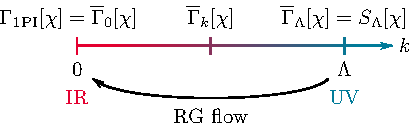
\includegraphics{frg/figures/frg_flow.pdf}%
\end{center}%
	\caption{%
		Sketch of the \acrshort{frg} flow of the \acrshort{eaa} $\FSeaa_k[\FSsf]$ from its initial condition $S_\Lambda[\FSsf]$ in the \acrshort{uv} ($k=\Lambda$) towards the full quantum \acrshort{ea} in the \acrshort{ir} ($k\rightarrow 0$).%
	}%
	\label{fig:rg_scetch}%
\end{figure}%
Before a discussion of the \frg{} on a technical level (culminating in the derivation and discussion of the central \frgEquation{} in \cref{subsec:wetterich}), we will outline the idea behind this powerful non-perturbative method.
The \frg{} implements Kenneth G. Wilson's non-perturbative continuum \rg{} approach~\cite{Wilson:1971bg,Wilson:1971dh,Wilson:1979qg} in momentum space and thus by extension the discrete equivalent \dash{} position space based \dash{} \rg{} concept of Leo P. Kadanoff's block-spin transformations~\cite{Kadanoff:1966wm}.
The conceptual idea behind the \rg{} is the study of physical systems/theories at different scales.
The \grg \footnote{%
	We use \acrshort{grg} when making statements which apply for the functional renormalization group as well as for the non-perturbative renormalization group in general.%
} can be used to study the scale evolution of a theory from a microscopic scale \dash{} where the theory is initially defined using microscopic interactions \dash{} to a macroscopic scale \dash{} where we can compute macroscopic observables and correlation functions of the physical system under consideration.
The changes during scale evolution in the correlation functions and observables of a field theory are governed by quantum and/or thermodynamic fluctuations.
Considering a functional formulation of \qft{} based on a suitable functional integral, Wilson's \rg{} approach is based on integrating out fluctuations step by step \dash{} momentum shell by momentum shell.
This incremental study of successive \rg{} steps facilitates the practical computation of the underlying functional integral, which is usually not possible when trying to incorporate all fluctuations at once.

The \frg{} describes the \rgscaleevolution{} of a scale-dependent \eaa{} $\FSeaa_k[\FSsf]$ as a series of infinitesimal \rg{} steps in form of a so-called \rg{} flow.
See \cref{fig:rg_scetch} for a pictographic sketch of this process.
In the following we use $k$ to denote the \rgscale{}.
The starting point of the \frg{} flow is $\FSeaa_\Lambda[\FSsf]$ which is based on an Euclidean action $S_\Lambda[\FSsf]$ at a \rg{} \uv{} initial scale $k=\Lambda$.
The action at this scale is considered ``classical'' in a sense that either $\Lambda$ is asymptotically large or $S_\Lambda[\FSsf]$ includes all quantum fluctuations with momenta $|p|>\Lambda$.
Starting at the initial scale $\Lambda$ the idea is to integrate out fluctuations successively in a Wilsonian manner by splitting the quantum fields based on their momenta.
In the \frg{} this is achieved by introducing a suitable regulator which ultimately implements and facilitates this process.
The \rgscaleevolution{} in the \frg{} is governed by one central non-perturbative one-loop equation \dash{} the so-called \textit{Wetterich} flow equation~\cite{\frgWetterichEq}.
This non-linear functional differential equation is exact given a suitable regulator choice and thus maps the problem of solving the functional integral to solving a corresponding flow equation.
Using this flow equation, one can track the change of a microscopic theory with a given action $\FSeaa_\Lambda[\FSsf]=S_\Lambda[\FSsf]$ in the \uv{} ($k=\Lambda$) towards a macroscopic theory with a full quantum effective action $\FSeaa_0[\FSsf]=\Gamma_\mathrm{1PI}[\FSsf]$ in the \ir{}~(${k\rightarrow 0}$).
The \frg{} is inherently non-perturbative and thus allows the study of both weakly and strongly coupled systems.
Using the scale-dependent \eaa{} $\FSeaa_k[\FSsf]$ it is in principle possible to study the ground state, realized symmetries, thermodynamic properties, and correlation functions of a theory at varying  \rgscales{} $k$. 
This makes the \frg{} an immensely powerful tool to study the effect of quantum and/or thermodynamic fluctuations in a wide range of physical systems at different scales in a controlled and unified framework.

\subsection{Scale-dependent generating functionals}\label{subsubsec:generatingFunctionals}
We begin our technical discussion of the \frg{} by introducing two auxiliary scale-dependent generating functionals.

For the following discussion we consider a quantum field theory with the Euclidean action $\Sinit[\FSff{\FSsf}]$, where $\FSff{\FSsf}$ is a multi component fundamental quantum field which includes the entire field content of the theory under consideration in the \fs{} notation of \cref{app:FS}.
In the subsequent derivation we consider a generic theory in which $\FSff{\FSsf}$ collects scalar (mesonic) fields $\FSff{\MFphi}$ and Grassmann-valued (fermionic) fields $\FSff{\MFpsi}$ and $\FSff{\MFpsib}$:
\begin{align}
	(\FSffd{\FSsf}{a})\equiv (\FSff{\MFphi},\FSff{\MFpsi},\FSff{\MFpsib})\,.
\end{align}

We further introduce $\FSf{\FSsf}$ as a \rgscaledependent{} multi component composite field of the fundamental fields
\begin{align}
	(\FSfd{\FSsf}{a})\equiv (\FSf{\FSsf}_{k;\FSidx{a}}[\FSff{\FSsf}])\,.
\end{align}
For readability we will usually suppress the scale and functional dependency in the notation.
We introduce corresponding sources
\begin{align}
	(\FSfd{J}{a})\equiv (\FSf{J}_{\MFphi},\FSf{J}_{\MFpsib}, \FSf{J}_{\MFpsi})
\end{align}
in the generating functional to extract correlation functions and to study condensation.
Working with such scale-dependent composite fields as degrees of freedom is more elegant and efficient since the fundamental fields of a theory are not necessary suitable degrees of freedom at all scales.
A prime example for this is \qcd{}, where the fundamental fields are quarks and gauge fields which are excellent degrees of freedom in the \uv{} (at some \uv{} reference scale $\Lambda$) due to asymptotic freedom.
In the \ir{} ($k\rightarrow0$) however \dash{} due to confinement and chiral symmetry breaking \dash{} a description in terms of hadrons is desirable, since baryons and mesons are the relevant degrees of freedom.
Introducing those hadrons as composite fields of the fundamental fields has proven highly effective and elegant in \frg{} studies of \qcd{}, see, \eg{}, \ccite{Alkofer:2018guy,Fu:2019hdw,Fu:2022gou} and references therein and \cref{subsec:chiralLEFT}.

To implement Wilson's \rg{} approach we introduce a \rgscaledependent{} regulator term $\Delta S_k[\FSf{\FSsf}]$ in the Euclidean generating functional of the theory under consideration
\begin{align}
	Z_k[\FSf{J}]=\exp\del[3]{-\Delta S_k\sbr{\frac{\delta}{\delta \FSf{J}}}}Z[\FSf{J}]= \int \mathcal{D}[\FSff{\FSsf}] \exp\del{-\Sinit[\FSff{\FSsf}]-\Delta S_k[ \FSf{\FSsf}]+\FSfu{J}{m}\FSfd{\FSsf}{m}}\,,
	\label{eq:ZkDef}
\end{align}
where $\Sinit[\FSff{\FSsf}]$ is the Euclidean, classical action prescribing kinematics and interactions of the fundamental fields $\FSff{\FSsf}$. 
$\mathcal{D}[\FSff{\FSsf}]$ is a suitable functional integral measure including a possible normalization factor $\mathcal{N}$ and appropriate boundary conditions for the fields when working at non-zero temperature, see \cref{app:thermalQFT} for details.
Such a normalization factor $\mathcal{N}$ is arbitrary, since it does not affect observables and thus varies depending on the conventions used for $Z[\FSf{J}]$.
General expectation values in presence of $\FSf{J}$ and $\Delta S_k[\FSf{\FSsf}]$  are given by
\begin{align}
	\expectationValue{O[\FSf{\FSsf}]}{\FSf{J}} =\frac{1}{Z_k[\FSf{J}]}  \int \mathcal{D}[\FSff{\FSsf}]\, O[\FSf{\FSsf}] \exp\del{-\Sinit[\FSff{\FSsf}]-\Delta S_k[ \FSf{\FSsf}]+\FSfu{J}{m}\FSfd{\FSsf}{m}}
	\label{eq:expectationOJ}\,.
\end{align}
From \cref{eq:expectationOJ} one obtains the useful identity
\begin{align}
	\frac{\delta}{\delta \FSfu{J}{a}}\expectationValue{O[\FSf{\FSsf}]}{\FSf{J}} = -\expectationValue{\FSfd{\FSsf}{a}}{\FSf{J}}\expectationValue{O[\FSf{\FSsf}]}{\FSf{J}} + \expectationValue{\FSfd{\FSsf}{a}O[\FSf{\FSsf}]}{\FSf{J}}
	\label{eq:dexpectationOJdJ}\,.
\end{align}
For practical computations in the scope of this work it is convenient to choose a regulator term $\Delta S_k[ \FSf{\FSsf}]$ which  is quadratic in the fields
\begin{align}
	\Delta S_k[ \FSf{\FSsf}] 
	\equiv  \Delta S[ \FSf{\FSsf},R_k]
	\equiv \frac{1}{2} \FSregulator{\FSidx{m},\FSidx{n}}\FSfd{\FSsf}{n}\FSfd{\FSsf}{m}\,,\label{eq:DeltaSRab}
\end{align}
where we introduced the regulator $\FSregulator{\FSidx{m},\FSidx{n}}$\footnote{%
	We have chosen $\frac{1}{2} \FSregulator{\FSidx{m},\FSidx{n}}\FSfd{\FSsf}{n}\FSfd{\FSsf}{m}$ and not $\FSregulator{\FSidx{n},\FSidx{m}}\FSfd{\FSsf}{n}\FSfd{\FSsf}{m}$ like in \ccite{Pawlowski:2005xe} out of personal preference especially related to the form of \cref{eq:DeltaSab}.%
}.
$\Delta S_k[ \FSf{\FSsf}] $ should appear as a scalar in the exponent under the functional integral. This implies a bilinear form of the regulator for Grassmann-valued FS components with 
\begin{align}
	\FSregulator{\FSidx{m},\FSidx{n}} = \FSc{\FSidx{n},\FSidx{m}} \FSregulator{\FSidx{n},\FSidx{m}}
\end{align}
and a non-trivial structure in its internal spaces. A quadratic regulator leads to one-loop flow equations for all \nptFunctions{}~\cite{Litim:2002xm,Pawlowski:2005xe}.
Higher-order regulators are possible, see, \eg{}, \ccite{Pawlowski:2005xe}, but will not be discussed in our work.
With the definition \eqref{eq:DeltaSRab} the second FS derivative of the regulator term is given by
\begin{align}
	\Delta S[ \FSf{\FSsf},R_k]_{,\FSidx{a}\FSidx{b}}
	=\frac{1}{2} \frac{\delta}{\delta \FSfd{\FSsf}{a}}\frac{\delta}{\delta \FSfd{\FSsf}{b}}\FSregulator{\FSidx{m},\FSidx{n}}\FSfd{\FSsf}{n}\FSfd{\FSsf}{m}
	=\frac{1}{2} \frac{\delta}{\delta \FSfd{\FSsf}{a}}\del{
	\FSregulator{\FSidx{m},\FSidx{b}}\FSfd{\FSsf}{m}+\FSc{\FSidx{b},\FSidx{n}}\FSregulator{\FSidx{b},\FSidx{n}}\FSfd{\FSsf}{n}
	}
	=\FSregulator{\FSidx{a},\FSidx{b}}\,.\label{eq:DeltaSab}
\end{align}
We will discuss further constraints on the regulator related to the proper implementation of Wilson's \rg{} approach in \cref{subsubsec:regulator}.

The scale-dependent Schwinger functional $W_k[\FSf{J}]$ is given by 
\begin{align}
	W_k[\FSf{J}] = \ln Z_k[\FSf{J}]\,.\label{eq:WkDef}
\end{align}
Considering functional derivatives of the Schwinger functional leads to connected \nptFunctions{}, see, \eg{}, \ccite{Iliopoulos:1974ur,ZinnJustin:2002ru,Weinberg:1996kr,Peskin:1995ev,PawlowskiScript}. The one-point function \dash{} the expectation value of $\FSf{\FSsf}$ in presence of $\Delta S_k[ \FSf{\FSsf}]$ and $\FSf{J}$ \dash{} is simply given by
\begin{align}
	\frac{\delta}{\delta \FSfu{J}{a}}W_k[\FSf{J}] = \frac{1}{Z_k[\FSf{J}]}\frac{\delta Z_k[\FSf{J}]}{\delta\FSfu{J}{a}}=\expectationValue{\FSfd{\FSsf}{a}}{\FSf{J}}\,.\label{eq:dWkdJa}
\end{align}
To study the \rgscale{} evolution of $W_k[\FSf{J}]$ and by extension $Z_k[\FSf{J}]$ we consider the total \rg-scale derivative\footnote{%
	Total derivatives \wrt{} the \acrshort{rg} scale (\acrshort{rg} time) will be frequently abbreviated by $\partial_k$ ($\partial_t$) in the following.
	We denote \acrshort{rg} scale-dependence with either $k$ or $t$ depending on the element and context.
	In terms of derivatives both are always understood as $k(t)$ and $t(k)$.
	The reasoning behind this mixed use of $k$ and $t$ in formulas is that for the discussion of flow/evolution we like $t$ while for denoting \acrshort{ir} and \acrshort{uv} we prefer $k$.%
} of $W_k[\FSf{J}]$.
It is convenient to study and discuss the scale evolution from $k=\Lambda$ to $k\rightarrow0$ using a dimensionless \rg/flow time $t$ which we define\footnote{%
	We adopt a sign convention for the \rg{} flow time resulting in a positive time evolution from the \uv{} ($k=\Lambda\Leftrightarrow t=0$) to the \ir{} ($k \rightarrow 0 \Leftrightarrow t\rightarrow \infty$).
} as
\begin{align}
	&t \equiv - \ln \big( \tfrac{k}{\Lambda} \big) =  \ln \big( \tfrac{\Lambda}{k} \big) \, ,	\qquad	t \in [ 0, \infty ) \, .	\label{eq:def_rg_time}
\end{align}
The evolution equation for $W_k[\FSf{J}]$ is given by
\begin{align}
	\stepcounter{equation}\newSubEqBlock
	\dod{W_k[\FSf{J}]}{t}&=\dod{}{t}\ln Z_k[\FSf{J}]
	=\frac{1}{Z_k[\FSf{J}]}\dod{Z_k[\FSf{J}]}{t}\, = \subEqTag\\
	&=\frac{1}{Z_k[\FSf{J}]} \int \mathcal{D}[\FSff{\FSsf}]\, \dod{}{t}\exp\del{ -\Sinit[\FSff{\FSsf}] - \frac{1}{2} \FSregulator{\FSidx{m},\FSidx{n}}\FSfd{\FSsf}{n}\FSfd{\FSsf}{m} +\FSfu{J}{m}\FSfd{\FSsf}{m} }\, = \subEqTag\\
	&= \FSfu{J}{m}\expectationValue{\partial_t \FSfd{\FSsf}{m}}{\FSf{J}}-\frac{1}{2}\del{\partial_t \FSregulator{\FSidx{m},\FSidx{n}}}\expectationValue{\FSfd{\FSsf}{n}\FSfd{\FSsf}{m}}{\FSf{J}}- \FSregulator{\FSidx{m},\FSidx{n}}\expectationValue{\FSfd{\FSsf}{n}\partial_t\FSfd{\FSsf}{m}}{\FSf{J}}\label{eq:dWkdt},
\end{align}
where we considered $k=k(t)\equiv\Lambda\,\eu^{-t}$.
\Cref{eq:dWkdt} is the generalization of the Polchinski equation~\cite{Polchinski:1983gv} for composite fields with \ir{} regularization~\cite{PawlowskiScript}\footnote{%
	However, in the original work~\cite{Polchinski:1983gv} an effective action $L ( \Lambda, \phi )$ takes the role of $W_k[\FSf{J}]$ and it is formulated in terms of the fields $\phi$ instead of the sources $\FSf{J}$. For relations between the original Polchinski equation and the flow equations studied in this work and selected applications of the Polchinski equation, see, \eg{}, \ccite{Litim:2005us,Yabunaka:2018mju,Litim:2018pxe,Cotler:2022fze,Fu:2022gou}.
}.
We will discuss the scale-dependent Schwinger functional further in \cref{subsubsec:WtJd0} in the context of zero-dimensional \qfts{}.

\subsection{Scale-dependent effective average action}\label{subsec:frgeaa}
While working with \rg{} equations \eqref{eq:dWkdt} for the Schwinger functional is possible, it is more convenient for most practical computations to work with the scale-dependent \eaa{} $\FSeaa_k[\FSmf{\FSsf}]$  which is given by the modified Legendre transform of the Schwinger functional
\begin{align}
	\FSeaa_k[\FSmf{\FSsf}]&\equiv\FSea_k[\FSmf{\FSsf}] -\Delta S_k[\FSmf{\FSsf}] \equiv\sup_{\FSf{J}}\del{
	\FSfu{J}{m}\FSmfd{\FSsf}{m}-W_k[\FSf{J}]
	}-\Delta S_k[\FSmf{\FSsf}] \label{eq:Gammaksup}\, , \\
	\FSeaa_k[\FSmf{\FSsf}]+\Delta S_k[\FSmf{\FSsf}] &= \FSea_k[\FSmf{\FSsf}] = \FSmfu{J}{m}\FSmfd{\FSsf}{m}-W_k[\FSmf{J}]\, ,\label{eq:Gammak}
\end{align}
where we denote $\FSmfu{J}{m}$ as the source $\FSfu{J}{m}$ which realizes the supremum for a given so-called mean-field $\FSmfd{\FSsf}{m}$ and $\Delta S_k[\FSmf{\FSsf}]=\FSregulator{\FSidx{m},\FSidx{n}}\FSmfd{\FSsf}{n}\FSmfd{\FSsf}{m}/2$ in analogy to \cref{eq:DeltaSRab}.
The modification of the Legendre transform with $\Delta S_k[\FSmf{\FSsf}]$ is necessary in order to implement $\FSeaa_k\rightarrow S_\Lambda$ in the \uv{} limit $k\rightarrow \Lambda$, see \cref{subsubsec:zerodICS} for a detailed discussion of this subtle point. 
$\FSeaa_k[\FSmf{\FSsf}]$ is only guaranteed to be convex in the \ir{} ($k\rightarrow 0$)\footnote{%
	For certain theories and initial conditions for the \rgscaleevolution{} in a given truncation $\FSeaa_0[\FSmf{\FSsf}]=\FSea_0[\FSmf{\FSsf}]$ is only locally convex in the \ir{}. For details, see, \eg{}, \ccite{Litim:2006nn,Grossi:2019urj}. In this work we only consider theories with a convex effective action in the \ir{} limit.%
}, where $\Delta S_k[\FSmf{\FSsf}]\rightarrow 0$.
In this limit the \eaa{} reduces to the canonically known \ea{} $\FSea_0[\FSmf{\FSsf}]\equiv\Gamma_\mathrm{1PI}[\FSmf{\FSsf}]$, see, \eg{}, \ccite{Peskin:1995ev}.
The \eaa{} $\FSeaa_k[\FSmf{\FSsf}]$ is the scale-dependent generating functional of scale-dependent \ipi{} correlation functions, see, \eg{}, \ccite{Iliopoulos:1974ur,ZinnJustin:2002ru,Weinberg:1996kr,Peskin:1995ev,PawlowskiScript}, which in the \ir{} limit $k\rightarrow 0$ reduce to the canonical \ipi{} correlation functions of the full quantum field theory.
As such $\FSeaa_k[\FSmf{\FSsf}]$ encodes the entire information of a theory without diagrammatic redundancies.
In the \ir{} it also encodes the thermodynamic \textit{grand potential} $\thermalGrandPotential$, see \cref{app:grandCanonicalPartitionFunction} and especially \cref{eq:thermalGrandPotential} for details, and thus can be used to study thermodynamic properties, phase transitions, and symmetry breaking, \cf{} \cref{chap:GN,chap:QMM} for explicit applications.

By construction \cref{eq:Gammak} implies
\begin{align}
	\frac{\delta}{\delta \FSfu{J}{a}}\del{\FSeaa_k[\FSmf{\FSsf}]+\Delta S_k[\FSmf{\FSsf}] }=0&=\frac{\delta}{\delta \FSfu{J}{a}}\sup_{\FSf{J}}\del[3]{
	\FSfu{J}{m}\FSmfd{\FSsf}{m}-W_k[\FSf{J}]
	}
	=\sup_{\FSf{J}}\del[3]{
	\FSmfd{\FSsf}{a}-\frac{\delta W_k[\FSf{J}]}{\delta\FSfu{J}{a}}},
\end{align}
which at the supremum $\FSf{J}=\FSmf{J}$ is equivalent to 
\begin{align}
\FSmfd{\FSsf}{a}=\eval[3]{\frac{\delta W_k[\FSf{J}]}{\delta\FSfu{J}{a}}}_{\FSf{J}=\FSmf{J}}\equiv \frac{\delta W_k[\FSmf{J}]}{\delta\FSmfu{J}{a}}\label{eq:dWdFSmfJ}
\end{align}
in accordance to \cref{eq:dWkdJa}.

The source realizing the supremum in \cref{eq:Gammaksup} is a scale-dependent functional of the mean-field, $\FSmfu{J}{a}\equiv \FSmf{J}_k^{\FSidx{a}}[\FSmf{\FSsf}]$, and in turn the mean-field as the expectation value of $\FSfd{\FSsf}{a}$ in presence of $\Delta S_k[\FSf{\FSsf}]$ and $\FSmf{J}$ is a scale-dependent functional of the source $\FSmf{J}$: $\FSmfd{\FSsf}{a}\equiv\FSmf{\FSsf}_{k;\FSidx{a}}[\FSmf{J}]\equiv \expectationValue{\FSfd{\FSsf}{a}}{\FSmf{J}}$.
We suppress the scale and functional-dependencies of $\FSmfu{J}{a}$ and $\FSmfd{\FSsf}{a}$ in our notation only for readability while still considering them in our computations, if not stated explicitly otherwise.
In the following we will mainly work with the source $\FSmf{J}$ and expressions evaluated at it.
Functionals and functional derivatives of $\FSmf{J}$ are to be understood as functionals and functional derivatives \wrt{} $\FSf{J}$ evaluated at $\FSf{J}=\FSmf{J}$ like in \cref{eq:dWdFSmfJ}.

\subsection{Quantum equation of motion and propagator}
Using the identity \eqref{eq:dWdFSmfJ} together with \cref{eq:Gammak} we derive the scale-dependent \qeom{}
\begin{align}
	\stepcounter{equation}\newSubEqBlock
	\frac{\delta}{\delta \FSmfd{\FSsf}{a}}\del[2]{\FSeaa_k[\FSmf{\FSsf}]+\Delta S_k[\FSmf{\FSsf}]}&= \frac{\delta}{\delta \FSmfd{\FSsf}{a}}\del[2]{ \FSmfu{J}{m}\FSmfd{\FSsf}{m}-W_k[\FSmf{J}] }\,=\subEqTag\\
	%&=\frac{\delta}{\delta \FSmfd{\FSsf}{a}}\del{\FSmfu{J}{m}\FSmfd{\FSsf}{m}}
	%-\frac{\delta W_k[\FSmf{J}]}{\delta \FSmfd{\FSsf}{a}}\\
	&= \frac{\delta \FSmfu{J}{m}}{\delta \FSmfd{\FSsf}{a}}\FSmfd{\FSsf}{m} + \FSc{\FSidx{a},\FSidx{m}}\FSmfu{J}{m}\frac{\delta \FSmfd{\FSsf}{m}}{\delta \FSmfd{\FSsf}{a}}  - \frac{\delta \FSmfu{J}{m}}{\delta \FSmfd{\FSsf}{a}} W_{k,\FSidx{m}}[J]\,=\subEqTag\\
	&= \FSc{\FSidx{a},\FSidx{m}}\FSd{a}{m}\FSmfu{J}{m}\,=\subEqTag \\
	&=  \FSgud{a}{m}\FSmfu{J}{m}\label{eq:QEOM}
\end{align}
relating sources $\FSmfu{J}{a}$ to their respective mean-fields $\FSmfd{\FSsf}{a}$.

Taking one additional derivative of $\FSmfd{\FSsf}{b} = W_{k,\FSidx{b}}[\FSmf{J}]$ \wrt{} $\FSmfu{J}{a}$ leads to the connected two-point function \dash{} the full scale-dependent propagator \dash{} in presence of the source $\FSmf{J}$ and regulator $\Delta S_k$:
\begin{align}
\FSpropagator{\FSidx{a},\FSidx{b}}[\FSmf{\FSsf}]&\equiv W_{k,\FSidxRow{\FSidx{a},\FSidx{b}}}[J]\\
\stepcounter{equation}\newSubEqBlock
&= \frac{\delta}{\delta \FSmfu{J}{a}} W_{k,\FSidx{b}}[J]= \frac{\delta}{\delta \FSmfu{J}{a}} \expectationValue{ \FSmfd{\FSsf}{b}}{\FSmf{J}}\equiv\FSmf{\FSsf}_{\FSidx{b},\FSidx{a}}=\subEqTag\\
&= \del{\frac{\delta}{\delta \FSmfu{J}{a}}  \frac{1}{Z_k[\FSmf{J}]}}\int \mathcal{D}[\FSff{\FSsf}] \, \FSfd{\FSsf}{b}\exp\del{\ldots} +
\frac{1}{Z_k[\FSmf{J}]}\int \mathcal{D}[\FSff{\FSsf}] \, \frac{\delta}{\delta \FSmfu{J}{a}} \FSfd{\FSsf}{b}\exp\del{\ldots}=\subEqTag\\
&= -\expectationValue{ \FSfd{\FSsf}{a}}{\FSmf{J}}\expectationValue{ \FSfd{\FSsf}{b}}{\FSmf{J}}
+ \FSc{\FSidx{a},\FSidx{b}} \expectationValue{ \FSfd{\FSsf}{b} \FSfd{\FSsf}{a}}{\FSmf{J}}=\subEqTag\\
&= \expectationValue{ \FSfd{\FSsf}{a} \FSfd{\FSsf}{b}}{\FSmf{J}[\FSsf]}-\FSmfd{\FSsf}{a} \FSmfd{\FSsf}{b}. \label{eq:Gkab}
\end{align}
The scale-dependent propagator $\FSpropagator{\FSidx{a},\FSidx{b}}[\FSmf{\FSsf}]$ is a fundamental object in the \frg{} due to its relation to the scale-dependent two-point function and since it connects functional derivatives \wrt{} $\FSmf{J}$ to the ones \wrt{} $\FSmf{\FSsf}$ via a chain rule
\begin{align}
 \frac{\delta}{\delta \FSmfu{J}{a}} =  \frac{\delta \FSmfd{\FSsf}{m}}{\delta \FSmfu{J}{a}}  \frac{\delta}{\delta \FSmfd{\FSsf}{m}}= \FSpropagator{\FSidx{a},\FSidx{m}}[\FSmf{\FSsf}]\frac{\delta}{\delta \FSmfd{\FSsf}{m}}\label{eq:GchainRule},
\end{align}
which, when applied to $\FSmfd{\FSsf}{a}$, yields
\begin{align}
 \frac{\delta \FSmfd{\FSsf}{b}}{\delta \FSmfu{J}{a}} = \FSpropagator{\FSidx{a},\FSidx{b}}[\FSmf{\FSsf}] = \expectationValue{ \FSfd{\FSsf}{a} \FSfd{\FSsf}{b}}{\FSmf{J}}-\FSmfd{\FSsf}{a} \FSmfd{\FSsf}{b}\label{eq:Gexp}
\end{align}
in accordance to \cref{eq:dexpectationOJdJ}.

Taking one additional $\FSmf{J}$ derivative of the \qeom{} \eqref{eq:QEOM} and using the chain rule \eqref{eq:GchainRule} leads to the following relations between the scale-dependent propagator and the \eaa:
\begin{align}
	\stepcounter{equation}\newSubEqBlock
	\frac{\delta}{\delta\FSmfu{J}{a}}\frac{\delta \del[1]{\FSeaa_k[\FSmf{\FSsf}]+\Delta S_k[\FSmf{\FSsf}]}}{\delta \FSmfd{\FSsf}{b}}&=\FSgud{b}{m}\frac{\delta\FSmfu{J}{m}}{\delta\FSmfu{J}{a}}\, , \subEqTag\\
	\FSpropagator{\FSidx{a},\FSidx{m}}[\FSmf{\FSsf}]\frac{\delta}{\delta\FSmfd{\FSsf}{m}}\frac{\delta  \del[1]{\FSeaa_k[\FSmf{\FSsf}]+\Delta S_k[\FSmf{\FSsf}]}}{\delta \FSmfd{\FSsf}{b}}&= \FSgud{b}{m} \FSd{m}{a}\,,\subEqTag\\
	\FSpropagator{\FSidx{a},\FSidx{m}}[\FSmf{\FSsf}] \del{\FSvertex{\FSidx{m},\FSidx{b}}[\FSmf{\FSsf}]+\FSregulator{\FSidx{m},\FSidx{b}}}&= \FSgud{b}{a}\, , \label{eq:GkabImplicit}\\
	\stepcounter{equation}\newSubEqBlock
	\FSpropagator{\FSidx{a},\FSidx{c}}[\FSmf{\FSsf}] &= \FSgud{n}{a} \del[1]{\FSeaa_k[\FSmf{\FSsf}]+\Delta S_k[\FSmf{\FSsf}]}_{\FSidxRow{\FSidx{n},\FSidx{c}}}^{-1}\,,\subEqTag\\
	\FSgud{n}{a}\FSpropagator{\FSidx{n},\FSidx{c}}[\FSmf{\FSsf}] &=  \del[1]{\FSeaa_k[\FSmf{\FSsf}]+\Delta S_k[\FSmf{\FSsf}]}_{\FSidxRow{\FSidx{a},\FSidx{c}}}^{-1}\,,\subEqTag
\end{align}
with
\begin{align}
\del[1]{\FSvertex{\FSidx{a},\FSidx{n}}[\FSmf{\FSsf}]+\FSregulator{\FSidx{a},\FSidx{n}}}\del[1]{\FSeaa_k[\FSmf{\FSsf}]+\Delta S_k[\FSmf{\FSsf}]}_{\FSidxRow{\FSidx{n},\FSidx{b}}}^{-1}&\equiv \FSd{a}{b}.
\end{align}
The relation between the full scale-dependent propagator and the inverse Hessian of $\FSeaa_k[\FSmf{\FSsf}]+\Delta S_k[\FSmf{\FSsf}]$ includes a contraction with $\FSgud{n}{a}$ which results in a minus sign for the propagators of Grassmann-valued fields\footnote{%
	It is very common in literature to absorb this minus sign in a so-called super-trace denoted by $\mathrm{STr}$. We will retain the minus sign for Grassmann-valued fields in their propagators.%
}.

\subsection{The Wetterich equation}\label{subsec:wetterich}
Using the expressions derived in the previous subsections we are now able to derive the central equation of the \frg{} \dash{} the Wetterich flow equation governing the \rg{}-scale/\rg{}-time evolution of the \eaa{}. 
The total \rgtime{} derivative of the \eaa{} can be computed by combining \cref{eq:dWkdt,eq:Gammak}:
\begin{align}
	\stepcounter{equation}\newSubEqBlock
	\dod{}{t} \FSeaa_k[\FSmf{\FSsf}] &= 
		\dod{}{t}\!\del{\FSmfu{J}{m}\FSmfd{\FSsf}{m}-W_k[\FSmf{J}] -\Delta S_k[\FSmf{\FSsf}]}\,= \subEqTag\label{eq:wgcfA}\\ % definition eq:Gammak
	&=\del{\partial_t\FSmfu{J}{m}}\FSmfd{\FSsf}{m}
		+\FSmfu{J}{m}\partial_t\FSmfd{\FSsf}{m}
		-\eval[0]{\partial_t}_{\FSmf{J}}W_k[\FSmf{J}]
		-\del{\partial_t\FSmfu{J}{m}}W_{k,\FSidx{m}}[\FSmf{J}]\,-\notag\\
		&\qquad-\frac{1}{2}\del{\partial_t \FSregulator{\FSidx{m},\FSidx{n}}}\FSmfd{\FSsf}{n}\FSmfd{\FSsf}{m}
		-\FSregulator{\FSidx{m},\FSidx{n}}\FSmfd{\FSsf}{n}\partial_t\FSmfd{\FSsf}{m}\,= \subEqTag\label{eq:wgcfB}\\ % d\dt derivative
	&=\del{\partial_t\FSmfu{J}{m}}\del{\FSmfd{\FSsf}{m}-W_{k,\FSidx{m}}[\FSmf{J}]}
		+\FSmfu{J}{m}\partial_t\FSmfd{\FSsf}{m}\,-\notag\\
		&\qquad-\FSmfu{J}{m}\expectationValue{\partial_t \FSfd{\FSsf}{m}}{\FSmf{J}}+\frac{1}{2}\del{\partial_t \FSregulator{\FSidx{m},\FSidx{n}}}\expectationValue{\FSfd{\FSsf}{n}\FSfd{\FSsf}{m}}{\FSmf{J}}+ \FSregulator{\FSidx{m},\FSidx{n}}\expectationValue{\FSfd{\FSsf}{n}\partial_t\FSfd{\FSsf}{m}}{\FSmf{J}}\,-\notag\\
	&\qquad-\frac{1}{2}\del{\partial_t \FSregulator{\FSidx{m},\FSidx{n}}}\FSmfd{\FSsf}{n}\FSmfd{\FSsf}{m}
		-\FSregulator{\FSidx{m},\FSidx{n}}\FSmfd{\FSsf}{n}\partial_t\FSmfd{\FSsf}{m}\,= \subEqTag\label{eq:wgcfC}\\ % definition eq:dWkdt
	%&= \del{\partial_t\FSmfu{J}{m}}\del{\FSmfd{\FSsf}{m}-W_{k,\FSidx{m}}[\FSmf{J}]}
		%+\FSmfu{J}{m}\del{\partial_t\FSmfd{\FSsf}{m}-\expectationValue{\partial_t \FSfd{\FSsf}{m}}{\FSmf{J}}}\,+\notag\\
		%&\qquad+\frac{1}{2}\del{\partial_t \FSregulator{\FSidx{m},\FSidx{n}}}\expectationValue{\FSfd{\FSsf}{n}\FSfd{\FSsf}{m}}{\FSmf{J}}
		%+\FSregulator{\FSidx{m},\FSidx{n}}\expectationValue{\FSfd{\FSsf}{n}\partial_t\FSfd{\FSsf}{m}}{\FSmf{J}}\,-\notag\\
		%&\qquad-\frac{1}{2}\del{\partial_t \FSregulator{\FSidx{m},\FSidx{n}}}\FSmfd{\FSsf}{n}\FSmfd{\FSsf}{m}
		%-\FSregulator{\FSidx{m},\FSidx{n}}\FSmfd{\FSsf}{n}\partial_t\FSmfd{\FSsf}{m}= \subEqTag\\
	&=\FSmfu{J}{m}\del{\partial_t\FSmfd{\FSsf}{m}-\expectationValue{\partial_t \FSfd{\FSsf}{m}}{\FSmf{J}}}
		+\frac{1}{2}\del{\partial_t\FSregulator{\FSidx{m},\FSidx{n}}}\FSpropagator{\FSidx{n},\FSidx{m}}[\FSmf{\FSsf}]\,+\notag\\
		&\qquad+\FSregulator{\FSidx{m},\FSidx{n}}\del{\expectationValue{\FSfd{\FSsf}{n}\partial_t \FSfd{\FSsf}{m}}{\FSmf{J}}-\FSmfd{\FSsf}{n}\partial_t\FSmfd{\FSsf}{m}}\,= \subEqTag\label{eq:wgcfD}\\ % eq:dWdFSmfJ and eq:Gexp
	&=\frac{1}{2}\del{\partial_t\FSregulator{\FSidx{m},\FSidx{n}}}\FSpropagator{\FSidx{n},\FSidx{m}}[\FSmf{\FSsf}]+\FSmfu{J}{m}\del{\partial_t\FSmfd{\FSsf}{m}-\expectationValue{\partial_t \FSfd{\FSsf}{m}}{\FSmf{J}}}\,+\notag\\
		&\qquad+\FSregulator{\FSidx{m},\FSidx{n}}\del{\frac{\delta}{\delta\FSmfu{J}{n}}\expectationValue{\partial_t \FSfd{\FSsf}{m}}{\FSmf{J}}+\FSmfd{\FSsf}{n}\del{\expectationValue{\partial_t \FSfd{\FSsf}{m}}{\FSmf{J}}-\partial_t\FSmfd{\FSsf}{m}}} \subEqTag\label{eq:wgcfE}\\ % eq:dexpectationOJdJ
	\dod{}{t} \FSeaa_k[\FSmf{\FSsf}] &=\frac{1}{2}\del{\partial_t\FSregulator{\FSidx{m},\FSidx{n}}}\FSpropagator{\FSidx{n},\FSidx{m}}[\FSmf{\FSsf}]+\del{\FSmfu{J}{m}+\FSregulator{\FSidx{m},\FSidx{n}} \FSmfd{\FSsf}{n}}\del{\partial_t\FSmfd{\FSsf}{m}-\expectationValue{\partial_t \FSfd{\FSsf}{m}}{\FSmf{J}}}\,+\notag\\
		&\qquad+\FSregulator{\FSidx{m},\FSidx{n}}\FSpropagator{\FSidx{n},\FSidx{l}}[\FSmf{\FSsf}]\frac{\delta \expectationValue{\partial_t \FSfd{\FSsf}{m}}{\FSmf{J}}}{\delta \FSmfd{\FSsf}{l}}\,,\label{eq:WetterichGeneralCompositeFields}
\end{align}
where we used the identities \eqref{eq:dWdFSmfJ} and \eqref{eq:Gexp} in \cref{eq:wgcfD}, the identity \eqref{eq:dexpectationOJdJ} in \cref{eq:wgcfE}, and the chain rule \eqref{eq:GchainRule} to ultimately obtain \cref{eq:WetterichGeneralCompositeFields}.
Enforcing the constraint
\begin{align}
\expectationValue{\partial_t \FSfd{\FSsf}{m}}{\FSmf{J}}=\partial_t\FSmfd{\FSsf}{m} \label{eq:dFSfdkConstraint}
\end{align}
on the composite field $\FSfd{\FSsf}{m}$ simplifies the scale evolution equation for $\FSeaa_k$ significantly. \Cref{eq:dFSfdkConstraint} introduces additional constraints which resolve the scale evolution of $\FSf{\FSsf}$ in terms of the $\FSff{\FSsf}$~\cite{Pawlowski:2005xe}.
Working with the evolution equation for $\FSeaa_k[\FSmf{\FSsf}]$ does not require an explicit resolution of the evolution $\partial_t\FSf{\FSsf}_{t;\FSidx{a}}[\FSff{\FSsf}]$ of the composite quantum fields $\FSf{\FSsf}_{t;\FSidx{a}}[\FSff{\FSsf}]$ in terms of the microscopic, fundamental fields $\FSff{\FSsf}$, see \ccite{Pawlowski:2005xe,PawlowskiScript,Fu:2019hdw,FuQCDRev,Ihssen:2023nqd} for more details.
Therefore we encode the theory in $\FSeaa_k[\FSmf{\FSsf}]$ completely in terms of mean-fields $\FSmf{\FSsf}$, consider \cref{eq:dFSfdkConstraint} as the defining property of $\FSf{\FSsf}_{k;\FSidx{a}}[\FSff{\FSsf}]$, and eliminate all dependencies on $\partial_t\FSfd{\FSsf}{m}$ on the level of the \eaa{} using \cref{eq:dFSfdkConstraint}. Using the constraint \eqref{eq:dFSfdkConstraint} simplifies the scale evolution \eqref{eq:WetterichGeneralCompositeFields} for $\FSeaa_k$ to
\begin{align}
\dod{}{t} \FSeaa_k[\FSmf{\FSsf}] = \eval[0]{\partial_t}_{\FSmf{\FSsf}}\!\FSeaa_k[\FSmf{\FSsf}]+ \FSeaa_k^{,\FSidx{m}}[\FSmf{\FSsf}]\,\partial_t\FSmfd{\FSsf}{m} =\frac{1}{2}\del{\partial_t\FSregulator{\FSidx{m},\FSidx{n}}}\FSpropagator{\FSidx{n},\FSidx{m}}[\FSmf{\FSsf}]
+\FSregulator{\FSidx{m},\FSidx{n}}\FSpropagator{\FSidx{n},\FSidx{l}}[\FSmf{\FSsf}]\frac{\delta \partial_t \FSmfd{\FSsf}{m}}{\delta \FSmfd{\FSsf}{l}}\label{eq:WetterichGeneral}\,.
\end{align}
This is the \rg{} evolution/Wetterich equation of $\FSeaa_k[\FSsf]$ for general scale-dependent mean-fields $\FSsf_k$, \cf{} \ccite{Gies:2006wv,Rennecke:2015lur,Ihssen:2023nqd}, sometimes also referred to as \textit{Flow Equation with Dynamical Hadronization}~\cite{Braun:2014ata,PawlowskiScript} in the context of \qcd{}.
To close the system \eqref{eq:WetterichGeneral} the (flow of) the composite field $(\partial_t)\FSmfd{\FSsf}{m}[\FSsf]$ has to be specified.
This generalized version of the Wetterich equation for composite fields is an extremely powerful tool to study strongly interacting theories with emerging, relevant degrees of freedom \dash{} like \qcd{} \dash{} \cf{} \ccite{Cyrol:2017ewj,Alkofer:2018guy,Fu:2019hdw,FuQCDRev} and \cref{paragraph:qcdDynHad}.

For our computational studies within this work, which do not include explicit composite fields, this general equation can be simplified further by considering only linear scale-dependencies in $\partial_t\FSmf{\FSsf}_{k;\FSidx{m}}$ solely governed by an appropriate, field-independent wave-function renormalization:
\begin{align}
\FSmf{\FSsf}_{k;\FSidx{m}} = \del[1]{Z^{\FSsf}_{k;\FSidx{m}}}^{1/2} \FSmf{\FSsf}_{0;\FSidx{m}} \Rightarrow \partial_t\FSmf{\FSsf}_{k;\FSidx{m}} = \eta^{\FSsf}_{k;\FSidx{m}} \FSmf{\FSsf}_{k;\FSidx{m}}\,,\label{eq:dFSmfdtLinear}
\end{align}
with the anomalous dimension
\begin{align}
\eta^{\FSsf}_{k;\FSidx{m}}  \equiv \frac{1}{2}\partial_t \ln Z^{\FSsf}_{k;\FSidx{m}}  = \frac{1}{2}\frac{\partial_t Z^{\FSsf}_{k;\FSidx{m}} }{Z^{\FSsf}_{k;\FSidx{m}}}.\label{eq:etaChi}
\end{align}
Using \cref{eq:dFSmfdtLinear} the general evolution \cref{eq:WetterichGeneral} simplifies to
\begin{alignat}{2}
	\dod{}{t} \FSeaa_k[\FSmf{\FSsf}] &= \eval[0]{\partial_t}_{\FSmf{\FSsf}}\!\FSeaa_k[\FSmf{\FSsf}]+ \FSeaa_k^{,\FSidx{m}}[\FSmf{\FSsf}]\,\eta^{\FSsf}_{k;\FSidx{m}}\FSmfd{\FSsf}{m} &&=\frac{1}{2}\del{\partial_t\FSregulator{\FSidx{m},\FSidx{n}}}\FSpropagator{\FSidx{n},\FSidx{m}}[\FSmf{\FSsf}]
	+\FSregulator{\FSidx{m},\FSidx{n}}\FSpropagator{\FSidx{n},\FSidx{l}}[\FSmf{\FSsf}]\eta^{\FSsf}_{k;\FSidx{l}}=\notag\\
	&=\del[3]{\eval[0]{\partial_t}_{\FSmf{\FSsf}}+\eta^{\FSsf}_{k;\FSidx{m}}\FSmfd{\FSsf}{m}\frac{\delta}{\delta \FSmfd{\FSsf}{m}} }\FSeaa_k[\FSmf{\FSsf}]&&=\frac{1}{2}\FSpropagator{\FSidx{m},\FSidx{n}}[\FSmf{\FSsf}]\del[3]{\partial_t+2\eta^{\FSsf}_{k;\FSidx{n}}}\FSregulator{\FSidx{n},\FSidx{m}}\, ,\label{eq:WetterichEta}
\end{alignat}
which we refer to as the Wetterich equation for the scale-dependent mean-field $\FSmf{\FSsf}_{k;\FSidx{m}}$.
The simple scale-dependence of \cref{eq:dFSmfdtLinear} can be absorbed into the \eaa{} by switching variables from $\FSmf{\FSsf}_{k;\FSidx{m}}$ to $\FSmf{\FSsf}_{0;\FSidx{m}}$ (which we will denote as $\FSmf{\FSsf}_{\FSidx{m}}$ in the following for simplicity/readability) thus considering an \eaa{} for the bare mean-fields with the wave-function renormalizations $Z^{\FSsf}_{k;\FSidx{m}}$ absorbed
into the couplings within $\FSeaa_k[\FSsf_0\equiv\FSsf]$.
This simplifies \cref{eq:WetterichEta} even further to the Wetterich equation~\cite{\frgWetterichEq} in its well known form
\begin{align}
	\partial_t\FSeaa_k[\FSsf]
	%FRG`wetterichEq`FS0[{1}][[1]]
	=\frac{1}{2}\ncm{\FSpropagator{\FSidx{m},\FSidx{n}}[\FSsf],\FSregulatorDt{\FSidx{n},\FSidx{m}}}
	\equiv \FRGflow_k[\FSsf]
	=\frac{1}{2}\,\begin{gathered}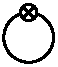
\includegraphics{frg/diagrams/FRG-wetterichEq-FS0_1_1.pdf}\end{gathered}\label{eq:WetterichEq}\,,
\end{align}
where we still use \fs{} notation (instead of a super-trace) for a unified treatment of fermionic (Grassmann-valued) and bosonic (non-Grassmann-valued) fields collected in $\FSsf$ as well as our \rgtime{} derivative with $k=k(t)\equiv \Lambda\eu^{-t}\Rightarrow \partial_t\rightarrow -k\partial_k$.

Recalling \cref{eq:GkabImplicit} we note that the propagator $\FSpropagator{\FSidx{a},\FSidx{b}}[\FSsf]$ on the \rhs{} of the \frgEquation{} depends on the inverse Hessian of $\FSeaa_k[\FSsf]+\Delta S_k[\FSsf]$ and thus on the second functional derivatives of $\FSeaa_k[\FSsf]$.
Therefore the Wetterich equation manifests as a non-linear functional differential equation for the \eaa{}.
The \rhs{} of \cref{eq:WetterichEq} is a non-perturbative one-loop equation since it involves the full scale-dependent propagator $\FSpropagator{\FSidx{a},\FSidx{b}}[\FSsf]$ (solid black line in diagrams) of the theory contracted with the regulator insertion $\FSregulatorDt{\FSidx{b},\FSidx{a}}$ (black cross within a circle in diagrams).
In \cref{eq:WetterichEq} we further introduced the symbolic abbreviation $\FRGflow_k[\FSsf]$\footnote{%
	Note that through the propagator $\FRGflow_k[\FSsf]$ is a non-linear functional of $\FSeaa_k[\FSsf]$ \dash{} its matrix of second functional derivatives/two-point functions to be precise \dash{} and of the regulator, \ie{}, $\FRGflow_k[\FSsf]\equiv\FRGflow_k[\FSeaa_k,R_k;\FSsf]$.
	Symbolic integration of the \frgEquation{} over the \frg{} flux $\FRGflow_k[\FSsf]$ in \rgtime{} is to be understood as solving the functional differential equation in \rgtime{}.%
} for the \textit{\frg{} flux} on the \rhs{}, which will be particularly useful in \cref{subsec:RGconsistency}.
The \frgEquation{} is the governing master equation of the \frg{} framework and it can be used as a generating equation for explicit flow equations for higher-order \nptFunctions{}, see \cref{subsec:higherOrderFlowEquations} for details.

\subsubsection{Regulators, initial condition, and implementation of Wilson's RG approach}\label{subsubsec:regulator}
For the subsequent discussions, regarding the regulator and \ic{} for the Wetterich equation, the following functional integral representation \eqref{eq:EEAint} for the \eaa{} $\FSeaa_k[\FSmf{\FSsf}]$ will be useful.
Using \cref{eq:Gammak} with the definitions \eqref{eq:ZkDef} and \eqref{eq:WkDef} for $Z_k$ and $W_k$ respectively we arrive at
\begin{align}
\stepcounter{equation}\newSubEqBlock
\eu^{-\FSeaa_k[\FSmf{\FSsf}]}
%&=\int\mathcal{D}[\FSff{\FSsf}] \exp\del[3]{-\Sinit[\FSff{\FSsf}]-\Delta S_k[ \FSff{\FSsf}]+\FSmfu{J}{m}\FSffd{\FSsf}{m} +\Delta S_k[ \FSmf{\FSsf}]- \FSmfu{J}{m}\FSmfd{\FSsf}{m} }\\
&= \int \mathcal{D}[\FSff{\FSsf}] \exp\Big(-\Sinit[\FSff{\FSsf}]+\FSmfu{J}{m}\del{\FSffd{\FSsf}{m}-\FSmfd{\FSsf}{m}} 
-\frac{1}{2}\FSregulator{\FSidx{m},\FSidx{n}}\del{\FSffd{\FSsf}{n}\FSffd{\FSsf}{m}-\FSmfd{\FSsf}{n}\FSmfd{\FSsf}{m}}
\Big)\,=\subEqTag \label{eq:EEAintA}\\
%&= \int \mathcal{D}[\FSff{\FSsf}] \exp\del[3]{-\Sinit[\FSmf{\FSsf}+\FSff{\FSsf}]+\FSmfu{J}{m}\FSffd{\FSsf}{m}
%-\frac{1}{2}\FSregulator{\FSidx{m},\FSidx{n}}\del{\del{\FSmfd{\FSsf}{n}+\FSffd{\FSsf}{n}}\del{\FSmfd{\FSsf}{m}+\FSffd{\FSsf}{m}}-\FSmfd{\FSsf}{n}\FSmfd{\FSsf}{m}}
%}\\
&=\int \mathcal{D}[\FSff{\FSsf}] \exp\Big(-\Sinit[\FSmf{\FSsf}+\FSff{\FSsf}]+\FSmfu{J}{m}\FSffd{\FSsf}{m}
-\frac{1}{2}\FSregulator{\FSidx{m},\FSidx{n}}\FSffd{\FSsf}{n}\FSffd{\FSsf}{m} -\FSregulator{\FSidx{m},\FSidx{n}}\FSffd{\FSsf}{n}\FSmfd{\FSsf}{m}
\Big)\,=\subEqTag\label{eq:EEAintB}\\
&=\int \mathcal{D}[\FSff{\FSsf}] \exp\Big(-\Sinit[\FSmf{\FSsf}+\FSff{\FSsf}]+\FSeaa_k^{,\FSidx{m}}[\FSmf{\FSsf}]\FSffd{\FSsf}{m}+\FSffd{\FSsf}{m}\Delta S_k^{,\FSidx{m}}[\FSmf{\FSsf}]\,-\notag\\
&\qquad\qquad\qquad\qquad\qquad\qquad\qquad\qquad-\frac{1}{2}\FSregulator{\FSidx{m},\FSidx{n}}\FSffd{\FSsf}{n}\FSffd{\FSsf}{m} -\FSregulator{\FSidx{m},\FSidx{n}}\FSffd{\FSsf}{n}\FSmfd{\FSsf}{m}
\Big)\subEqTag \label{eq:EEAintC}\\
%&=\int \mathcal{D}[\FSff{\FSsf}] \exp\del[3]{-\Sinit[\FSmf{\FSsf}+\FSff{\FSsf}] - \Delta S_k[\FSff{\FSsf}] +\FSffd{\FSsf}{m}\FSeaa_k^{,\FSidx{m}}[\FSmf{\FSsf}]+\FSffd{\FSsf}{m}\FSregulator{\FSidx{n},\FSidx{m}}\FSmfd{\FSsf}{n}
 %-\FSregulator{\FSidx{m},\FSidx{n}}\FSffd{\FSsf}{n}\FSmfd{\FSsf}{m}
%}\\
\eu^{-\FSeaa_k[\FSmf{\FSsf}]}&=\int \mathcal{D}[\FSff{\FSsf}] \exp\bigg(-\Sinit[\FSmf{\FSsf}+\FSff{\FSsf}] - \Delta S_k[\FSff{\FSsf}] +\frac{\delta\FSeaa_k[\FSmf{\FSsf}]}{\delta \FSmfd{\FSsf}{m}}\FSffd{\FSsf}{m} 
\bigg)\,\label{eq:EEAint}
\end{align}
where we shifted the integration variable according to $\FSff{\FSsf}\rightarrow \FSff{\FSsf} +\FSmf{\FSsf}$ in \cref{eq:EEAintA} and eliminated the source realizing the supremum $\FSmf{J}$ by means of the \qeom{} \eqref{eq:QEOM} in \cref{eq:EEAintC}.\bigskip

In the following we will discuss the necessary properties of the regulator $R_k^{\MFphi\MFphi}(p^2)$,
\begin{align}
R_k^{\FSf{\MFphi}_p,\FSf{\MFphi}_{p'}}=R_k^{\FSf{\MFphi}\FSf{\MFphi}}(p^2)(2\piu)^d\delta^{(d)}(p-p')\equiv p^2 r(p^2/k^2) (2\piu)^d\delta^{(d)}(p-p'),
\end{align}
related to the implementation of Wilson's \rg{} approach for the bosonic FS components in $d$ dimensions, \cf{} \cref{app:fourier} for related conventions.
Regulators related to Grassmann-valued field components inherit similar properties modulo some modifications accounting for internal structure. In the end we will always use a unified regulator scheme for all fields completely specified by a regulator shape function $r(y)$ with the dimensionless ratio 
\begin{align}
	y\equiv \frac{p^2}{k^2},
	\label{eq:yofpkDef}
\end{align}
of the momentum squared to the \rgscale{} squared.

Inserting regulator terms $\Delta S$ in the generating functionals of quantum field theories is not unique to the \frg{}.
Similar or in certain limits even equivalent flow equations to the Wetterich equation in fact preceded it.
Prominent examples are the Wegner-Houghton equation of the seminal paper~\cite{Wegner:1972ih} or the functional variant~\cite{Symanzik:1971cu,Symanzik:1971vw,Alexandre:2000eg} of the well known Callan-Symanzik equation~\cite{Callan:1970yg,Symanzik:1970rt}.
The specific properties of the regulator insertion put forward with the Wetterich equation~\cite{\frgWetterichEq} distinguishes the \frg{} from earlier (functional) \rg{} approaches.
Certain constraints on $R_k$ (or $r(y)$ respectively) are imperative to the correct and explicit implementation of Wilson's non-perturbative continuum \rg{} approach~\cite{Wilson:1971bg,Wilson:1971dh,Wilson:1979qg} outlined in the introduction of this \cref{sec:FRG}.
Only a suitable regulator choice enables sensible computations in the \frg{} approach for a theory at hand.

The four major constraints on $R_k^{\FSf{\MFphi}\FSf{\MFphi}}(p^2)$ are:
\begin{enumerate}
	\item \phantomsection\label{paragraph:regulatorIR}\textbf{Infrared finiteness:}
	\begin{align}
	\lim_{p^2/k^2\rightarrow 0 }R_k^{\FSf{\MFphi}\FSf{\MFphi}}(p^2)>0 \qquad (\text{typically }\sim k^2).\label{eq:RkBIR}
	\end{align}
	The quadratic ansatz \eqref{eq:DeltaSRab} together with the requirement of \cref{eq:RkBIR} introduces a mass term (typically $\sim k^2$) for the low momentum modes, $p^2<k^2$, of $\FSf{\MFphi}$. This additional mass term suppresses fluctuations of those low momentum components in the functional integral \eqref{eq:ZkDef} and regularizes the theory in the \ir{}.
	
	\item \phantomsection\label{paragraph:regulatorHighP}\textbf{Vanishing for high momentum modes:} For fields with momenta larger than the current scale, $p^2>k^2$ the regulator has to vanish in the limit
	\begin{align}
	\lim_{p^2/k^2\rightarrow \infty }R_k^{\FSf{\MFphi}\FSf{\MFphi}}(p^2)=0 \label{eq:RkBUV}
	\end{align}
	in $d$ dimensions at least with $(p^2)^{(d-1)/2}R_k(p^2)\rightarrow 0$~\cite{Pawlowski:2015mlf,PawlowskiScript}. 
	This property implies for $k\rightarrow 0$ \dash{} in the physical limit \dash{} that all regulator-dependencies drop out and all generating functionals ($Z_k$, $W_k$ and $\FSeaa_k$) include the full effect of all quantum fluctuations.
	In other words, the introduction of a suitable regulator does not spoil the physical \ir{} observables extracted from these generating functionals at $k\rightarrow 0$.
	The requirement of \cref{eq:RkBUV} implies in the \uv{}, $p^2/k^2\gg 1$, the vanishing of the \rgscale{} derivative $\partial_k R_k^{\FSf{\MFphi}\FSf{\MFphi}}(p^2)$, which ensures \uv{} finiteness.
	Regulators fulfilling \cref{eq:RkBIR,eq:RkBUV} typically have a \rg{}-scale derivative $\partial_k R_k^{\FSf{\MFphi}\FSf{\MFphi}}(p^2)$ which peaks around the momentum shell $p\sim k$ and thus the contributions from fields with momenta $\sim k$ dominate in the functional integral. This notion of momentum locality of \rg{} steps implements Wilson's non-perturbative \rg{} approach~\cite{Wilson:1971bg,Wilson:1971dh,Wilson:1979qg} of integrating out fluctuations momentum shell by momentum shell. 
	
	\item \phantomsection\label{paragraph:regulatorUV}\textbf{Diverging in the ultraviolet:} For $k\rightarrow \Lambda$, where $\Lambda$ is an \uv{} initial scale which should be larger than all relevant physical scales of the problem at hand, the regulator should diverge
	\begin{align}
	\lim_{k\rightarrow \Lambda} R_k^{\FSf{\MFphi}\FSf{\MFphi}}(p^2)=\infty.
	\end{align}
	This can be discussed explicitly for the \eaa{} $\FSeaa_k$ using its integral representation \eqref{eq:EEAint}: the regulator insertion $\Delta S_k[\FSff{\FSsf}]$ in \eqref{eq:ZkDef} diverges for $k\rightarrow \Lambda$ and thus dominates the functional integral on the \rhs{}
	In this limit $\Delta S_k[\FSff{\FSsf}]$ acts as a functional delta distribution~\cite{Wetterich:2001kra,Gies:2006wv} and the functional integral on the \rhs{} of \cref{eq:EEAint} can be evaluated to $\exp(-\Sinit[\FSmf{\FSsf}])$.
	Subsequently the \rgscaledependent{} \eaa{} $\FSeaa_\Lambda[\FSmf{\FSsf}]$ at the \uv{} initial scale $\Lambda$ reduces to the classical action $\Sinit[\FSmf{\FSsf}]$.
	
	Depending on the theory at hand, the explicit choice of regulator (shape function), and the chosen \uv{} initial scale $\Lambda$, the simple identification of a plain classical action $S[\FSmf{\FSsf}]$ as \ic{} at $k=\Lambda$ for $\FSeaa_k[\FSmf{\FSsf}]$ might be insufficient especially when working with a finite \uv{} initial scale $\Lambda$.
	Subtleties related to the chosen normalization of generating functionals, renormalization procedure, and potentially gauge fixing might require the addition of suitable (counter) terms at $k=\Lambda$ and thus a modified \ic{} $S_\Lambda[\FSmf{\FSsf}]$, see, \eg{}, \ccite{Pawlowski:2005xe,PawlowskiScript,Braun:2018svj}. 
	The concept of renormalization group consistency discussed in \cref{subsec:RGconsistency} is closely related to the proper choice of $S_\Lambda[\FSmf{\FSsf}]$.
	We will discuss problem/theory specific subtleties further when we introduce the \ics{} for the explicit \frg{} flows considered within this work.
	See, \eg{}, \cref{paragraph:ONRGconsistency}, \cref{subsec:UUV}, and \cref{sec:cdwmf}.
	
	\item \phantomsection\label{paragraph:regulatorSym}\textbf{Symmetry considerations:} The regulator should not break any symmetries of the theory, \ie{}, its functional integral.
	Prime examples of such symmetries are chiral or $O(N)$ symmetries and for the relativistic theories considered here \Poincare{} invariance.
	If a regulator choice breaks such a symmetry computed observables might be spoiled by this artificial, explicit symmetry breaking.
	This situation might be remedied by introducing appropriate counter terms in $S_\Lambda[\FSmf{\FSsf}]$, \cf{} \cref{subsec:renomMF}, or in case of the breaking of gauge symmetry by a more elaborate construction, \cf{} \cref{paragraph:qcdGF}.
\end{enumerate}

The first three constraints related to the finiteness \dash{} proper regularization and \ic{} for the \frg{} flow \dash{} in practice often compete with symmetry considerations like \Poincare{} invariance and related causality issues (unphysical poles in the complex frequency plane) arising during analytical continuation to real time quantities, for details, see, \eg{}, Sec. II of \ccite{Braun:2022mgx} and references therein.
Furthermore, computational and numerical practicability considerations can conflict with especially symmetry considerations.
A prime example of the latter is the use of purely spatial regulators in our computations of \cref{chap:GN,chap:QMM} which introduces an explicit breaking of \Poincare{} invariance. 
The use of purely spatial regulators is mainly motivated by the facilitation or at least significant simplification of computations at non-zero temperature.

An explicit choice of regulator (shape function) is usually made weighing the different constraints and practicability/feasibility considerations.
Common and in some cases even established regulator choices often strongly vary depending on the problem at hand, the employed truncation, \cf{} \cref{subsubsec:truncation}, and scope of the investigation.
Further details on the vast and important topic of adequate regulator choice in the \frg{} framework can be found in \ccite{Litim:2000ci,Litim:2001up,Pawlowski:2005xe,Rosten:2010vm,Osborn:2011kw,Pawlowski:2015mlf,Braun:2017srn,Braun:2020bhy,DePolsi:2022wyb,Otto:2022jzl,Braun:2022mgx,Ihssen:2023xlp,Zorbach:2024zjx} and references therein.

\fullWidthFigure%
	{frg/figures/regulator_shape_functions.pdf}% Graphics
	[fig:rShape_plain,fig:rShape_derivative]% Sublabels
	{%
		Plots of selected \dash{} \cf{} \cref{eq:rflat,eq:rsharp,eq:rlambdaDef} \dash{} regulator shape functions on the left \subref{fig:rShape_plain} and their derivatives on the right \subref{fig:rShape_derivative}.
		In terms of its properties the exponential regulator (shape function) $r_\mathrm{exp}(y)$ may be considered as an archetypical \frg{} regulator implementing Wilson's \rg{} approach with a smooth focusing around $p=k$ and many sketches of \frg{} regulators, see, \eg{}, Fig. 1 of \ccite{Gies:2006wv}, resemble its plot here.%
	}%Caption
	{fig:rShape}%Label
In this work we will employ regulators related to three explicit regulator shape functions (presented in the notation of Table 1 of \ccite{Pawlowski:2015mlf}): the flat (\acrshort{lpa} optimized Litim) regulator~\nbcite{Litim:2000ci,Litim:2001up}
\begin{align}
	r_\mathrm{flat}(y)\equiv\del{\frac{1}{y}-1}\mkern-1.5mu\thetaLitim(1-y)\,,
\label{eq:rflat}
\end{align}
the step-like sharp regulator
\begin{align}
	r_\mathrm{sharp}(y)\equiv\frac{c}{y}\mkern1.5mu\thetaLitim(1-y)\,,
\label{eq:rsharp}
\end{align}
in the limit $c\rightarrow\infty$, and the exponential regulator
\begin{align}
	r_\mathrm{exp}(y)\equiv\del{\exp(y)-1}^{-1}\,.
\label{eq:rexp}
\end{align}
When working with these shape functions it is convenient to define 
\begin{align}
	\lambda(y)\equiv r(y)+1
	\label{eq:rlambdaDef}
\end{align}
as well as fermionic $\rf(y)$ and bosonic $\rb(y)$ shape functions related by
\begin{align}
	\lambda(y)\equiv r(y)+1\equiv \rb(y)+1\equiv(\rf(y)+1)^2\, .
	\label{eq:rfrbDef}
\end{align}
The three shape functions and their derivatives are visualized in \cref{fig:rShape}.
The particular choice of how the shape functions \eqref{eq:rflat}--\eqref{eq:rexp} and their derivatives are plotted in \cref{fig:rShape} is based on their appearance in explicit expressions, \cf{} \cref{eq:cdwFlow,eq:cdwFlow}.
This visualization complements the discussion of finiteness and the related first three constraints on $R_k^{\FSf{\MFphi}\FSf{\MFphi}}(p^2)$ which can be directly translated to constraints\footnote{%
	The constraints \cref{eq:ryA,eq:ryC} \dash{} \textit{infrared finiteness} and \textit{diverging in the ultraviolet} \dash{} are on the level of the regulator shape function $r(y)$ closely linked.
	Indeed considering ${\lim_{y\rightarrow 0 } y\, r(y)=1}$ entails $r(y)\rightarrow1/y$ and thus guarantees \cref{eq:ryC} in the limit $y\rightarrow0$.
} for the shape functions, \cf{} \ccite{Pawlowski:2015mlf},
\begin{subequations}\label{eq:ry}
\begin{align}
	\lim_{y\rightarrow 0 } y\, r(y)&>0\qquad (\text{typically }1)\,,\label{eq:ryA}\\
	\lim_{y\rightarrow \infty,\,\epsilon>0 } y^{\frac{d}{2}+\epsilon}r(y)&=0\,,\label{eq:ryB}\\
	\lim_{y\rightarrow 0 } r(y)&=\infty\,.\label{eq:ryC}
\end{align}
\end{subequations}
The flat regulator shape function is optimized~\cite{Litim:2000ci,Litim:2001up} for \acrshort{lpa} computations, \cf{} \cref{subsubsec:truncation}, in the sense that this regulator choice maximizes the gap in the inverse propagator which according to \ccite{Litim:2000ci} provides the greatest stability of the flow.
For additional details and a refined view of regulator optimization with a strong \cfd{} perspective we refer the interested reader to \ccite{Zorbach:2024zjx}.
Additionally the step function in \cref{eq:rflat} usually allows for a symbolic evaluation of momentum integrals and thus much simpler flow equations.
We will employ the flat and the sharp regulator shape functions in \cref{chap:GN}.
The latter is particularly useful in \mf{} computations since it also allows for a symbolic evaluation of momentum integrals and one usually recovers expressions known from conventional \mf{} computations with a sharp cutoff, \cf{} \cref{sec:gnInfInhomo} and, \eg{}, \ccite{Braun:2018svj}.
The exponential regulator shape function $r_\mathrm{exp}(y)$ is smooth and thus has certain advantages in explicit numerical computations, which we will leverage in \cref{chap:QMM}.

\subsubsection{Truncation and projection strategies}\label{subsubsec:truncation}
With a suitable regulator choice according to the previous \cref{subsubsec:regulator} the Wetterich equation is exact, hence the synonym \erg{} for \frg{}.
By construction the \ir{} physics, \ie{}, physical observables, are independent from the specific regulator choice as long as the regulator adheres to the previously established constraints.
Exact in this context means solving the evolution equations \eqref{eq:WetterichGeneral} or \eqref{eq:WetterichEq} with a suitable \ic{} and regulator choice from the \uv{} down to the \ir{} amounts to solving the underlying functional integral without any approximations.
The blue lines in \cref{fig:truncation} represent two exact \rg{} trajectories with different suitable regulators.
Using the full/untruncated Wetterich equation, the \ir{} physics encoded in $\FSeaa_0[\FSsf]$ is indeed regulator independent.
The \rg{} trajectories through theory space differ however for distinct regulators.
Flowing from $\FSeaa_\Lambda[\FSsf]$ to $\FSeaa_0[\FSsf]$, one gains access to the full quantum effective action $\FSeaa_0[\FSsf]=\Gamma_\mathrm{1PI}[\FSsf]$ and all related physical observables of the macroscopic theory prescribed by the microscopic action under consideration.

The issue a \frg{} practitioner faces however is one of \textit{conservation of complexity}: solving the underlying functional integral for strongly interacting theories is at best an extremely involved task and often practically impossible.
The functional flow equation for $\FSeaa_k[\FSsf]$ elegantly eliminates the need for the computation of the complicated functional integral at the cost of introducing a complicated functional differential equation to be solved.
Solving such equations without truncations or simplifying approximations is usually not possible for interacting \qfts{}, as there are no explicit numeric or symbolic methods to solve the arising non-linear functional differential equations.
One notable exception are applications of the \frg{} to models in zero dimensions, which will be discussed at length in \cref{chap:zeroONSU2}.
For theories in non-zero dimensions truncation schemes for the Wetterich equation are required to project from the full/exact functional differential equation onto a finite set of \pdes{} or even \odes{}.
For such differential equations numeric and in some cases even symbolic/analytic solution methods exist, which both facilitate practical computations in the \frg{} framework.
However with a truncation to a finite set of non-functional differential equations the \frg{} is no longer exact due to the simplifying steps taken and furthermore results computed in a truncation may explicitly depend on the specific regulator choice even for completely valid regulators.
This situation is visualized in \cref{fig:truncation} together with the untruncated/exact solution.
The red and green curves in \cref{fig:truncation} represent the flow using two different truncations: the regulator-dependence and derivation from the exact result for $\FSeaa_0[\FSsf]$ are clearly visualized in the \ir{} at $k=0$.
The truncation $t_2$ in \cref{fig:truncation} in green represent a systematic improvement over the truncation $t_1$ in red denoted by a weaker regulator-dependence and better error in the \ir{}.
Specifying errors related to truncation and regulator choice in the \frg{} can be extremely involved, especially when studying strongly interacting theories.
The process usually involves improving the truncation in a systematic way and comparing results obtained at varying levels of improvement to check for an apparent convergence of the chosen truncation and improvement scheme.

In the following we will briefly discuss four common truncation schemes. For details we refer to literature~\cite{Berges:2000ew,PawlowskiScript,Gies:2006wv,Kopietz:2010zz,Wetterich:2001kra,Pawlowski:2005xe,Rosten:2010vm,Delamotte:2007pf,Dupuis:2020fhh} and our applications in \cref{chap:zeroONSU2,chap:GN,chap:QMM}.
\fullWidthFigure%
	{frg/figures/truncation.pdf}% Graphics
	[]% Sublabels
	{Schematic \frg{} flow \dash{} \rgscaleevolution{} of the \eaa{} in the space of its couplings $\{\lambda_i\}$ for different regulators $R_1$ and $R_2$ (solid and dashed lines) and assuming an exact solution of the full Wetterich equation (blue lines) or solutions of the truncated Wetterich equation using two truncations $t_1$ and $t_2$ (red and green lines). Truncation $t_2$ is considered to be a systematic improvement of truncation $t_1$. }%Caption
	{fig:truncation}%Label

\paragraph{Vertex expansion}\phantomsection\label{paragraph:vertexExpansion}\mbox{} \\
Arguably the most natural truncation and expansion scheme for the \frgEquation{} is the so-called \textit{vertex expansion}.
The idea is to expand the \rgscaledependent{} \eaa{} $\FSeaa_k[\FSmf{\FSsf}]$ in its moments \dash{} in correlation functions \dash{} $\FSeaa_k^{(n)}(\FSmf{\FSsf}_0)$ around the expansion point $\FSmf{\FSsf}_0$ with
\begin{align}
\FSeaa_k[\FSmf{\FSsf}]\equiv\lim_{N\rightarrow\infty}\FSeaa_k^N[\FSmf{\FSsf}]\equiv\lim_{N\rightarrow\infty}\sum_{\{n\}=\{0\}}^{\{N\}} \FSeaa_k^{(n)}(\FSmf{\FSsf}_0)\prod_{i\in \{n\}}(\FSmf{\FSsf}_i-\FSmf{\FSsf}_{0,i})\,,\label{eq:vertexAnsatz}
\end{align}
where integration and summation over internal indices (position, flavor,$\ldots$) is implied and all \ipi{} vertices of theory are summed up in $\FSeaa_k^N[\FSmf{\FSsf}]$ up to order $N$.
Inserting the ansatz \eqref{eq:vertexAnsatz} into the \frgEquation{} one can use functional derivatives in the spirit of \cref{subsec:higherOrderFlowEquations} to generate an infinite tower of coupled \odes{} for all \ipi{} vertices
\begin{subequations}\label{eq:vertexTower}
\begin{align}
	\partial_t\FSeaa_k^{\{0\}}(\FSmf{\FSsf}_0)=&\,\FRGflow_k^{\{0\}}\mkern-3mu\del{\mkern2mu\FSeaa_k^{\{2\}};\FSmf{\FSsf}_0}\,,\\
	\partial_t\FSeaa_k^{\{1\}}(\FSmf{\FSsf}_0)=&\,\FRGflow_k^{\{1\}}\mkern-3mu\del{\mkern2mu\FSeaa_k^{\{2\}},\FSeaa_k^{\{3\}};\FSmf{\FSsf}_0}\,,\\
	\partial_t\FSeaa_k^{\{2\}}(\FSmf{\FSsf}_0)=&\,\FRGflow_k^{\{2\}}\mkern-3mu\del{\mkern2mu\FSeaa_k^{\{2\}},\FSeaa_k^{\{3\}},\FSeaa_k^{\{4\}};\FSmf{\FSsf}_0}\,,\\* % prohibits a page break here
	\vdots\mkern5mu&\notag
\end{align}
\end{subequations}
The \rhs{} of the flow equation for a \ipi{} vertex of order $n$ contains only the propagator $G_k$ (which non-linearly depends on the two-point functions), \ipi{} vertices up to order $n+2$, and the regulator insertion while maintaining one-loop structure.
We may also note that the zero-point function $\FSeaa_k^{(0)}(\FSmf{\FSsf}_0)$ does not couple back into the system.

One may expect good convergence of the tower of equations \eqref{eq:vertexTower}, if the higher-order \nptFunctions{} are suppressed.
Such a suppression motivates a truncation of the infinite tower up to order $N$ considering only $\FSeaa_k[\FSmf{\FSsf}]=\FSeaa_k^N[\FSmf{\FSsf}]$.
The infinite tower gets truncated up to order $N$ by either neglecting the flow of $\FSeaa_k^{\{N+1\}}(\FSmf{\FSsf}_0)$ and $\FSeaa_k^{\{N+2\}}(\FSmf{\FSsf}_0)$ or approximating the vertices, for the latter approach, see, \eg{}, \ccite{Blaizot:2005xy}.
When properly tracking the momentum dependence of the involved \ipi{} vertices, \cf{} the works~\cite{Blaizot:2004qa,Blaizot:2006vr, Blaizot:2006ak} of Jean-Paul Blaizot \etal{} and \ccite{Ledowski:2004zz,Sinner:2007ws,Kopietz:2010zz} of Peter Kopietz \etal{}, this approach provides excellent resolution in momentum space while having limited resolution in field space due to the expansion of the \eaa{} in \ipi{} vertices.
Due to the rapidly growing complexity of the flow equations when increasing $N$, practical computations are typically limited to a rather small order between $N=4$ and $N=6$.
The high resolution in momentum space and proper resolution of the momentum-dependence of the involved \ipi{} vertices makes the vertex expansion a very attractive expansion scheme for quantum many-particle systems in condensed matter physics, see, \eg{}, \ccite{Ledowski2004Jun,Benitez:2009xg,Boettcher:2012cm,Metzner2012Mar}, \hep{} and especially for Yang-Mills theories and \qcd{}, see, \eg{}, \ccite{Reuter:1993kw,Wetterich:1996kf,Gies:2002af,Braun:2014ata,Cyrol:2017ewj,Alkofer:2018guy,Fu:2019hdw}, and quantum gravity, see, \eg{}, \ccite{Reuter:1996cp,Christiansen:2015rva,Meibohm:2015twa,Eichhorn:2018akn,FuQCDRev}.
An overview and further relevant literature may be found in the Secs. 4, 5, and 6 of review~\cite{Dupuis:2020fhh}.
When studying symmetry breaking \dash{}  especially around phase transitions \dash{} the vertex expansion is of limited use since studies of such phenomena require a higher resolution in field space. 
Both symmetry breaking and also bound states can enhance higher-order \nptFunctions{} limiting or even destabilizing the vertex expansion, see also the discussion in the following paragraph \customref{paragraph:taylorExpansion}{Taylor and other global expansions}.
In this work we are mainly interested in the study of strongly coupled theories in field space and symmetry breaking in those systems. 
Thus we do not use the vertex expansion beyond the benchmark study of \cref{subsubsec:vertex_expansion,paragraph:sc2taylorFlow} in zero dimensions.

\paragraph{Derivative expansion and the local potential approximation}\phantomsection\label{paragraph:derivativeExpansion}\mbox{} \\
The main \frg{} expansion scheme employed in this work is the \de{}, which is a well established expansion and truncation scheme for the Wetterich equation in applications that require high resolution in field space, see, \eg{}, the review~\cite{Dupuis:2020fhh} and references therein.
Prime examples are the zero-dimensional theories we study in \cref{chap:zeroONSU2} and the \loefts{} we discuss in \cref{chap:GN,chap:QMM}.
The underlying idea behind the \de{} is to expand the \rgscaledependent{} \eaa{} $\FSeaa_k[\FSmf{\FSsf}]$ in powers of momenta \dash{} \ie{}, derivatives in position space, hence the name \de{}.
Such an expansion is justified when studying long range physics at small momentum scales $p^2$ satisfying
\begin{align}
	\frac{p^2}{s_k^2}\ll 1\,,
	\label{eq:deMomenta}
\end{align}
where $s_k$ is a theory specific \ir{} mass/momentum scale.
Even in theories without a physical mass gap $m_\gap$ the regulators used in the \frg{} provide an \ir{} regularization at finite $k$ and the characteristic scale $s_k$ is typically
\begin{align}
	s_k^2\approx m_\gap^2+k^2\,.
	\label{eq:dexikDef}
\end{align}
Considering the regulator properties discussed in \cref{subsubsec:regulator} we may indeed note that the regulator insertion $\partial_t R_k$ in the \frgEquation{} suppresses momenta $p^2\smallergtrsim k^2$ by focusing the integration over internal loop momenta around $p=k$, which is visualized in \cref{fig:rShape_derivative}.
The aforementioned suppression of high momentum modes renders the condition $p^2/k^2\smallerlesssim 1$ valid in the loop of the Wetterich equation.
This in turn implies that the condition~\eqref{eq:deMomenta} is indeed fulfilled \dash{} even for theories without a physical \ir{} mass gap $m_\gap$, \cf{} \cref{eq:dexikDef}.
A proper, \ie{}, for a given truncation optimized, regulator can greatly improve the stability and apparent convergence of the \de{}~\cite{Pawlowski:2005xe,Litim:2000ci,Litim:2001up}.
For the lowest-order \de{} \dash{} the so-called \acrrepeat{lpa}, which we will introduce in the following \dash{} the flat regulator that we introduced via its shape function in \cref{eq:rflat} is such an optimized regulator.

To illustrate the \de{} and related truncation strategies let us consider a theory of $N$ interacting scalar fields $\vec{\phi}$ with \ON{} symmetry in $d$ dimensions and corresponding mean-fields $\vec{\varphi}$ .
To lowest, zeroth-order \de{} \dash{} \ie{}, in \lpa{} \dash{} the \rgscaledependent{} \eaa{} is simply given by
\begin{align}
	\FSeaa_k^{\mathrm{DE}_0}\sbr{\vec{\varphi}\mkern2mu}\equiv\FSeaa_k^\mathrm{LPA}\sbr{\vec{\varphi}\mkern2mu}\equiv\int_x\del[3]{\frac{1}{2}\partial_\mu\varphi_i\partial_\mu\varphi_i+\Ukrho{}}\,,
	\label{eq:deLPA}
\end{align}
with $\varrho\equiv\varphi_i\varphi_i/2$ and the \rgscaledependent{}, \ON{}-symmetric self-interaction potential $\Ukrho{}$ as the only scale-dependent quantity.
Quantum fluctuations at $\order(\partial^2)$ and above are neglected and only the classical kinetic \dash{} without a running wave-function renormalization \dash{} is included~\cite{Reuter:1993rm,Morris:1994ki}.

The \rgscaledependent{} local potential can be evolved from the \uv{} at $k=\Lambda$ to the \ir{} $k\rightarrow 0$ using the \frgEq{}.
In the \ir{} $U_{k=0}\del{\varrho}$ can be identified with (contributes to) the effective potential $\VeffFArgs{\muT;\FSsf}$, see \cref{app:grandCanonicalPartitionFunction} and \cref{eq:VeffFdef}, when considering homogeneous (inhomogeneous) condensates. 
Thus $\Ukrho{}$ and especially $U_{k=0}\del{\varrho}$ play a critical role in the study of symmetry breaking and thermodynamics.
Further more the \lpa{} can be used for mean-field and large-$N$ computations, see, \eg{}, \cref{subsec:0dONresults,sec:gnInfInhomo,sec:gnInfHomo,sec:cdwmf}. 

The explicit flow equations for the local potential $\partial_t \Ukrho{}$ manifest in practice as \pdes{}, see, \eg{}, \cref{eq:pde_gamma,eq:flow_equation_effective_potential,eq:SU2model0dUFlow,eq:pdeq-U,eq:cdwFlow} in the main parts~\ref{chap:zeroONSU2}, \ref{chap:GN}, and \ref{chap:QMM} of this work.
As alluded to in the introduction~\ref{chap:introduction}, various collocation methods, \cf{} \ccite{\frgFDReferences,\frgSplineReferences} and also expansion schemes discussed in the \customref{paragraph:taylorExpansion}{next paragraph} are common and established in the \frg{} community to solve \lpa{} flow equations \dash{} the explicit \pdes{} for $\Ukrho{}$.
The \fd{} and spline collocation methods used, are however based on the often tacit assumption, that $\Ukrho{}$ is smooth.
This is however, as we argue at length in \cref{chap:zeroONSU2} and demonstrate also in \cref{chap:GN}, \apriori{} and also in prominent scenarios \aposteriori{}, in general not a valid assumption.
It has been established within the last few years by us and collaborators, \cf{} Refs.~\cite{Grossi:2019urj,zerod1,zerod2,zerod3,Ihssen2020,Grossi:2021ksl,Stoll:2021ori,Ihssen:2022xkr,Ihssen:2023xlp} and \cref{subsec:RGflow} as well as \cref{chap:zeroONSU2,chap:GN}, that the \frg{} flow equations \dash{} the \lpa{} flow equation as a truncated one, most prominently included \dash{} are non-linear conservation/convection equations.
Their non-linearity as well as explicit source/sink terms, \cf{} \cref{paragraph:chemical_potential_shock_wave}, can lead to discontinuities in $\partial_\MFrho \Ukrho{}$ and thus kinks in $\Ukrho{}$ which explains the poor (numerical) performance of the established ``grid methods''.
The adaptation of more suited numerical methods from the field of \cfd{}, see \cref{sec:conservationLaws}, is one major part of our research~\cite{zerod1,zerod2,zerod3,zerod4,Stoll:2021ori} discussed in \cref{chap:zeroONSU2,chap:GN}.\bigskip

The first systematic improvement $\mathrm{DE}_2$ in the \de{} to \lpa{}
\begin{align}
	\FSeaa_k^{\mathrm{DE}_2}\sbr{\vec{\varphi}\mkern2mu}=\int_x\del[3]{\frac{1}{2}Z_k(\varrho)\partial_\mu\varphi_i\partial_\mu\varphi_i+\frac{1}{4}Y_k(\varrho)\partial_\mu\varrho\partial_\mu\varrho+\Ukrho{}}\,,
	\label{eq:deDE2}
\end{align}
includes $\order(\partial^2)$ corrections in form of a field-dependent, running wave-function renormalization $Z_k(\varrho)$ and for $N>1$ an additional term $Y_k(\varrho)\partial_\mu\varrho\partial_\mu\varrho$ due to the difference in transverse and longitudinal fluctuations of $\vec{\varphi}$~\cite{Dupuis:2020fhh,Eser:2019pvd}. 
A very common simplification to $\mathrm{DE}_2$ is called \lpap{} which entails omitting the $Y_k(\varrho)$ contribution and considering only a field-independent $Z_k$.
Given an ansatz for the \eaa{} in \de{} one can proceed to compute the propagators in the given truncation.
The propagators and the ansatz for the \eaa{} can then be inserted into the \frgEquation{} and/or corresponding flow equations for higher-order \nptFunctions{} to project out flow equations for the running couplings.
Those flow equations manifest as \pdes{} or \odes{} allowing for a numerical solution of the Wetterich equation. 
Further details will be discussed in this thesis in \cref{chap:zeroONSU2,chap:GN,chap:QMM} while additional details and references can be found in, \eg{}, Sec. 2.3 of the review~\cite{Dupuis:2020fhh}.

\paragraph{\frg{} Taylor and other global expansions}\phantomsection\label{paragraph:taylorExpansion}\mbox{} \\
The so-called \textit{\frg{} Taylor expansion}, see, \eg{}, \ccite{\frgTaylorReferences}, is closely related to the \customref{paragraph:vertexExpansion}{vertex expansion} and the \lpa{} of the \customref{paragraph:derivativeExpansion}{derivative expansion}.
In the context of the \lpa{} the \frg{} Taylor expansion is simply the expansion of the \rgscaledependent{} local potential in a Taylor series
\begin{align}
	\Ukrho{}=\sum_{n=0}^{N_\nu} \frac{\lambda_{n,k}}{n!}\del{\MFrho-\kappa_k}^n\, ,\label{eq:ukrhoTaylor}
\end{align}
around a potentially scale-depended expansion point $\kappa_k$, with scale-depended moments $\lambda_{n,k}$ and an expansion order $N_\nu$, where we adopt the notation of \ccite{Fu:2022gou}.
Inserting the ansatz \nolinebreak[3]\eqref{eq:ukrhoTaylor} into the \lpa{} flow equation one can project onto the moments $\lambda_{n,k}$ and the expansion point $\kappa_k$ by taking derivatives \wrt{} $\MFrho.$
The \frg{} Taylor expansion includes the zeroth-order contributions in momentum space to the vertex expansion.
As such both \frg{} Taylor and vertex expansion are completely equivalent in zero-dimensional space-time, \cf{} \cref{subsubsec:vertex_expansion,paragraph:sc2taylorFlow}.

With a well chosen, potentially scale depended expansion point and sometimes a rather low number of expansion coefficients, the \frg{} Taylor expansion is an established method within the \frg{} community, see, \eg{}, the certainly incomplete list of \ccite{\frgTaylorReferences}.
However it is also acknowledged, that such a local expansion is rather limited in scenarios where global information about the potential is required, see, \eg{}, \ccite{Fu:2022gou,Pawlowski:2014zaa,PawlowskiScript}.
The study of symmetry breaking and phase transitions, especially first-order phase transitions, is one notable example.
It should however be noted, that an expansion like \cref{eq:ukrhoTaylor} and the projection onto its scale-dependent moments $\lambda_{n,k}$ and expansion point $\kappa_k$, \apriori{} assumes analyticity of $\Ukrho{}$ around the expansion point $\kappa_k$.
This is an incredibly restrictive and assumption that is just not justified for certain applications. 
We will discuss this limitation further in \cref{subsubsec:vertex_expansion,paragraph:sc2taylorFlow} in the context of our studies in zero dimensions.\bigskip

The local nature of the \frg{} Taylor expansion \eqref{eq:ukrhoTaylor} has, to an extent, motivated the adaptation of global pseudo-spectral collocation methods in the \frg{} community for an expansion of $\Ukrho{}$ in Chebyshev polynomials, see, \eg{}, \ccite{\frgChebyshevReferences}.
While this certainly improves upon the \frg{} Taylor expansion by considering a global expansion of the potential $\Ukrho{}$, such collocation methods are still severely limited when non-analyticities come into play.
The application of plain global pseudo-spectral collocation methods to non-linear convection equations including complicated source terms \dash{} like the \lpa{} flow equation \dash{} should be seriously reconsidered.
This is not the personal opinion of my collaborators and me, but rather firmly established knowledge in the field of such pseudo-spectral collocation methods.
It is interesting to note, that most of the aforementioned \frg{} Chebyshev literature references the excellent book \textit{``Chebyshev and Fourier Spectral Methods''}~\cite{boyd2001chebyshev} of John P. Boyd, which in no uncertain terms addresses the clear limitations of global-collocation methods when it comes to non-analyticities and shocks.
The praised exponential and geometric convergence of global-collocation methods is lost in presence of shocks, corner singularities, or discontinuities~\cite{boyd2001chebyshev}.
Spectral filtering, sequence acceleration, spectral reconstruction, or outright discontinuous Galerkin methods (employing pseudo-spectral methods in control volumes, allowing for discontinuities) are mentioned as necessary improvements when applying pseudo-spectral collocation methods to problems involving non-analyticities~\cite{boyd2001chebyshev}.
In plain pseudo-spectral collocation methods such non-analyticities manifest in the frequency spectrum as Wilbraham-Gibbs-type oscillations \nolinebreak[3]\cite{Wilbraham:1848,Gibbs:1898,Gibbs:1899} which without the aforementioned improvements completely destabilize the \ode{} system for the flow of the expansion coefficients.

\paragraph{Perturbative loop expansion}\phantomsection\label{paragraph:loopExpansion}\mbox{} \\
We will conclude the discussion on truncation strategies for the Wetterich equation with a short remark on the \textit{perturbative loop expansion} following \ccite{Papenbrock:1994kf,Litim:2002xm,Braun:2021retreat,PawlowskiScript,Gies:2006wv}.
Conventional renormalized perturbation theory, see, \eg{}, \ccite{Iliopoulos:1974ur,Peskin:1995ev,ZinnJustin:2002ru}, in form of a loop expansion in terms of classical, tree-level propagators can be recovered from the \frg{} in an iterative procedure. 
The $(N+1)$-loop correction to the \ea{} can be computed with the \frgEquation{} by inserting the $N$-loop expression for the propagator $G_k$ into the \rhs{} of \cref{eq:WetterichEq} and integrating the resulting equation from the \uv{} $k=\Lambda$ to the \ir{} $k=0$.

For the sake of simplicity we will consider a quantum field theory of a single scalar field $\phi$ with the classical action $S$ and corresponding mean-field $\varphi$ in the following.
Starting the iterative procedure with the zeroth-order tree-level propagator $G_k=(S^{(2)}+R_k)^{-1}$ and integrating over the \rgscale{}, one obtains the \ea{} to one-loop order
\begin{align}
	\Gamma_{1-\mathrm{loop}}[\varphi]=S[\varphi]+\FSeaa_{\Lambda,1}[\varphi]+\frac{1}{2}\Tr\ln S^{(2)}[\varphi]-\frac{1}{2}\Tr\ln \del[2]{S^{(2)}[\varphi]+R_\Lambda}\, ,
	\label{eq:ea1loop}
\end{align}
with the classical action $S[\varphi]$, a \rg{}-scheme-/regulator-dependent one-loop counter term $\FSeaa_{\Lambda,1}[\varphi]$, the potentially divergent one-loop diagram $\frac{1}{2}\Tr\ln S^{(2)}[\varphi]$, and the \rg{}-scheme-/regulator-dependent diagram $\frac{1}{2}\Tr\ln \del[1]{S^{(2)}[\varphi]+R_\Lambda}$ to cancel the potential divergences in the aforementioned diagram.
Thus the difference $\frac{1}{2}\Tr\ln S^{(2)}[\varphi]-\frac{1}{2}\Tr\ln \del[1]{S^{(2)}[\varphi]+R_\Lambda}$ can be considered as a regularized, finite loop diagram.
The counter term $\FSeaa_{\Lambda,1}[\varphi]$ can be determined by enforcing renormalization group consistency, see \cref{subsec:RGconsistency} for details, which in this context simply entails the independence of the \ea{} $\Gamma[\varphi]$ in the \ir{} of $\Lambda$.
The sum of the classical action and the counter term form the modified \ic{}: $\Sinit[\varphi]=S[\varphi]+\FSeaa_{\Lambda,1}[\varphi]$.

The two-loop result can be obtained by computing the propagator from the one-loop result~\eqref{eq:ea1loop}, inserting the result in the \rhs{} of the \frgEquation{} and again integrating over the \rgscale{}, see, \eg{}, \ccite{Litim:2002xm}.

Using the Wetterich equation as a master equation with the outlined iteration procedure is a simple and robust way to compute expressions for regularized and renormalized \ipi{} correlation functions to any desired perturbative loop-order.
The generation and complete resummation of the perturbative loop expansion also serves as further proof \dash{} beyond the validity and exactness of its derivation \dash{} that the \frgEquation{} is indeed exact.
A perturbative approach/loop expansion has only very limited applicability in the context of our work, since we are interested in strongly interacting systems which are notoriously elusive to tackle with such perturbative techniques. 
For discussions of perturbative results in the \frg{} context we refer the interested reader to, \eg{}, \ccite{Papenbrock:1994kf,Ellwanger:1997tp,Kopietz:2000bh,Codello:2015oqa,Codello:2017hhh}.

\subsection{Higher-order flow equations and their combinatorics in field space}\label{subsec:higherOrderFlowEquations}
Since practical computations of observables with the full \frgEq{} are for most theories impossible, truncations are employed to facilitate computations.
As a result $\FSeaa_k[\FSsf]$ is usually not accessible in its full functional form. 
The study and practical computation of moments of $\FSeaa_k[\FSsf]$  \dash{} higher-order \nptFunctions{} \dash{} however is still possible within the \frg{} framework.
To this end flow equations for higher-order \nptFunctions{} can be derived using the full \frgEq{} as a master equation.

Flow equations for higher-order \nptFunctions{} can be obtained by taking functional derivatives of the \frgEq{} \wrt{} external fields like $\FSmf{\FSsf} {}_{\FSidxE{x}}$\footnote{%
	We highlight external, \ie{}, non-contracted, \fs{}-indices with an underscore, \eg{}, $\FSidxE{x}$, in the context of higher-order flow equations for a clear distinction between contracted and external indices.
}.
Besides the vertices of the theory, the functional derivative of the propagator $\FSpropagator{\FSidx{a},\FSidx{c}}^{,\FSidxE{x}}$ is required.
An expression for $\FSpropagator{\FSidx{a},\FSidx{c}}^{,\FSidxE{x}}$ is obtained by computing the functional derivative of \cref{eq:GkabImplicit} explicitly:
\begin{align}
\frac{\delta}{\delta\FSmf{\FSsf} {}_{\FSidxE{x}}}\del{\FSpropagator{\FSidx{a},\FSidx{m}}[\FSmf{\FSsf}] \del{\FSvertex{\FSidx{m},\FSidx{b}}[\FSmf{\FSsf}]+\FSregulator{\FSidx{m},\FSidx{b}}}}&= \frac{\delta}{\delta\FSmf{\FSsf} {}_{\FSidxE{x}}}\FSgud{b}{a} =0\\[.1em]
\FSpropagator{\FSidx{a},\FSidx{m}}^{,\FSidxE{x}}[\FSmf{\FSsf}]\del{\FSvertex{\FSidx{m},\FSidx{b}}[\FSmf{\FSsf}]+\FSregulator{\FSidx{m},\FSidx{b}}}
&=-\FSc{\FSidxE{x},\FSidx{a}}\FSc{\FSidxE{x},\FSidx{m}}\FSpropagator{\FSidx{a},\FSidx{m}}[\FSmf{\FSsf}] \FSvertex{\FSidxE{x},\FSidx{m},\FSidx{b}}[\FSmf{\FSsf}] \\[.1em]
\FSpropagator{\FSidx{a},\FSidx{m}}^{,\FSidxE{x}}[\FSmf{\FSsf}]\FSd{c}{m}&= -\FSc{\FSidxE{x},\FSidx{a}}\FSpropagator{\FSidx{a},\FSidx{m}}[\FSmf{\FSsf}] \FSvertex{\FSidx{m},\FSidxE{x},\FSidx{n}}[\FSmf{\FSsf}]\del[1]{\FSeaa_k[\FSmf{\FSsf}]+\Delta S_k[\FSmf{\FSsf}]}_{\FSidxRow{\FSidx{n},\FSidx{c}}}^{-1} \\[.1em]
\stepcounter{equation}\newSubEqBlock
\FSpropagator{\FSidx{a},\FSidx{c}}^{,\FSidxE{x}}[\FSmf{\FSsf}]&= -\FSc{\FSidxE{x},\FSidx{a}}\FSpropagator{\FSidx{a},\FSidx{m}}[\FSmf{\FSsf}] \FSvertex{\FSidx{m},\FSidxE{x},\FSidx{n}}[\FSmf{\FSsf}] \FSgud{l}{n}\FSpropagator{\FSidx{l},\FSidx{c}}[\FSmf{\FSsf}] =\subEqTag\\[.1em]
&=
 -\FSc{\FSidxE{x},\FSidx{a}}\FSc{\FSidx{n},\FSidx{n}}\FSpropagator{\FSidx{a},\FSidx{m}}[\FSmf{\FSsf}] \FSvertex{\FSidx{m},\FSidxE{x},\FSidx{n}}[\FSmf{\FSsf}] \FSpropagator{\FSidx{n},\FSidx{c}}[\FSmf{\FSsf}]\,.\subEqTag
\end{align}
Diagrammatically taking the functional derivative of a propagator amounts to inserting a three-point vertex while accounting for potential sign changes due to the possible Grassmann-nature of the involved field components.
In a more compact form of our \fs{} notation we summarize at this point
\begin{align}
\frac{\delta }{\delta \FSmf{\FSsf} {}_{\FSidxE{x}}}\FSregulator{\FSidx{a},\FSidx{b}}&=
\big(\FSregulator{\FSidx{a},\FSidx{b}}\,\big)^{\mkern-1.5mu, \FSidxE{x}}=
0\, ,\label{eq:dRdchi0}\\[0.1em]
\frac{\delta }{\delta \FSmf{\FSsf} {}_{\FSidxE{x}}}\FSvertex{\FSidx{a},\ldots}&=
\FSvertex{\FSidxE{x},\FSidx{a},\ldots}=
\cm{\FSc{\FSidx{a},\FSidxE{x}},\FSvertex{\FSidx{a},\FSidxE{x},\ldots}}\, ,\label{eq:dGammadchi}\\[0.1em]
	\frac{\delta }{\delta \FSmf{\FSsf} {}_{\FSidxE{x}}}\FSpropagator{\FSidx{a},\FSidx{b}}&=
	\big(\FSpropagator{\FSidx{a},\FSidx{b}}\big)^{\mkern-1.5mu, \FSidxE{x}}	=-\cm{\FSc{\FSidxE{x},\FSidx{a},\FSidx{n},\FSidx{n}},\ncm{\FSpropagator{\FSidx{a},\FSidx{m}},\FSvertex{\FSidx{m},\FSidxE{x},\FSidx{n}},\FSpropagator{\FSidx{n},\FSidx{b}}}}\,.\label{eq:dGdchi}
\end{align}
Within \fs{} diagrams we use regular $n$-sided polygons with $n$ legs/lines to represent \fs{} vertices ${\protect\FSvertex{\protect\FSidx{x}_1,\ldots,\protect\FSidx{x}_n}}$.
Diagrams can be translated into their corresponding explicit mathematical expressions by reading off the involved elements \dash{} regulator insertion, propagators, and vertices \dash{} following the loop and vertex legs counter-clockwise starting at the regulator insertion which always includes the first and last \fs{} summation indices, see, \eg{}, \cref{eq:FS2_332_1,eq:FS2_332_2,eq:FS2_241_1} and \cref{eq:FS2_332_1-diagram,eq:FS2_332_2-diagram,eq:FS2_241_1-diagram}.

With \cref{eq:dRdchi0,eq:dGammadchi,eq:dGdchi} we are equipped to compute functional derivatives of the full \frgEq{}
\begin{align}
	\cm{2,\FSvertexDt{}}
	%FRG`wetterichEq`FS0[{1}][[1]]
	=\ncm{\FSpropagator{\FSidxI{a},\FSidxI{b}},\FSregulatorDt{\FSidxI{b},\FSidxI{a}}}
	=\begin{gathered}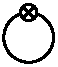
\includegraphics{frg/diagrams/FRG-wetterichEq-FS0_1_1.pdf}\end{gathered}\,,\label{eq:FS0}
\end{align}
starting with a \fs{} derivative \wrt{} the external (mean) field $\FSmf{\FSsf} {}_{\FSidxE{u}}$ we arrive at the flow equation for the one-point function
\begin{align}
	\cm{2,\FSvertexDt{\FSidxE{u}}}
	%FRG`wetterichEq`FS1[{2, {3, 1}}][[1]]
	=-\cm{\FSc{\FSidxE{u},\FSidxI{a},\FSidxI{c},\FSidxI{c}},\ncm{\FSpropagator{\FSidxI{a},\FSidxI{b}},\FSvertex{\FSidxI{b},\FSidxE{u},\FSidxI{c}},\FSpropagator{\FSidxI{c},\FSidxI{d}},\FSregulatorDt{\FSidxI{d},\FSidxI{a}}}}
	=-\cm{\FSc{\FSidxE{u},\FSidxI{a},\FSidxI{c},\FSidxI{c}}}\,\begin{gathered}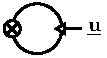
\includegraphics{frg/diagrams/FRG-wetterichEq-FS1_231_1.pdf}\end{gathered}\,.\label{eq:FS1}
\end{align}
An additional \fs{} derivative \wrt{} the external (mean) field $\FSmf{\FSsf} {}_{\FSidxE{v}}$ of \cref{eq:FS1} leads to the flow equation of the two-point function
\begin{align}
	\cm{2,\FSvertexDt{\FSidxE{v},\FSidxE{u}}}
	%*** Combinatorics
	&=\, \skeleton{T_{2,2}} + \skeleton{T_{2,1}} \,=\, \skeleton{2} + \skeleton{1} \label{eq:FS2}
	%*** FS expressions
	\newSubEqBlock\\[.25em]
	%FRG`wetterichEq`FS2[{3, {3, 2}}][[1]]
	&= \cm{\FSc{\FSidxE{u},\FSidxI{a},\FSidxE{v},\FSidxI{a},\FSidxI{c},\FSidxI{c},\FSidxI{e},\FSidxI{e}},\ncm{\FSpropagator{\FSidxI{a},\FSidxI{b}},\FSvertex{\FSidxI{b},\FSidxE{v},\FSidxI{c}},\FSpropagator{\FSidxI{c},\FSidxI{d}},\FSvertex{\FSidxI{d},\FSidxE{u},\FSidxI{e}},\FSpropagator{\FSidxI{e},\FSidxI{f}},\FSregulatorDt{\FSidxI{f},\FSidxI{a}}}} +  \subEqTag \label{eq:FS2_332_1}\\[.25em]
	%FRG`wetterichEq`FS2[{3, {3, 2}}][[2]]
	&\qquad + \cm{\FSc{\FSidxE{u},\FSidxE{v},\FSidxE{u},\FSidxI{a},\FSidxE{v},\FSidxI{a},\FSidxI{c},\FSidxI{c},\FSidxI{e},\FSidxI{e}},\ncm{\FSpropagator{\FSidxI{a},\FSidxI{b}},\FSvertex{\FSidxI{b},\FSidxE{u},\FSidxI{c}},\FSpropagator{\FSidxI{c},\FSidxI{d}},\FSvertex{\FSidxI{d},\FSidxE{v},\FSidxI{e}},\FSpropagator{\FSidxI{e},\FSidxI{f}},\FSregulatorDt{\FSidxI{f},\FSidxI{a}}}} - \subEqTag \label{eq:FS2_332_2}\\[.25em]
	%FRG`wetterichEq`FS2[{2, {4, 1}}][[1]]
	&\qquad -\cm{\FSc{\FSidxE{u},\FSidxI{a},\FSidxE{v},\FSidxI{a},\FSidxI{c},\FSidxI{c}},\ncm{\FSpropagator{\FSidxI{a},\FSidxI{b}},\FSvertex{\FSidxI{b},\FSidxE{v},\FSidxE{u},\FSidxI{c}},\FSpropagator{\FSidxI{c},\FSidxI{d}},\FSregulatorDt{\FSidxI{d},\FSidxI{a}}}} \subEqTag \label{eq:FS2_241_1}
	\newSubEqBlockPrime\\[.25em]
	%*** Diagrams
	&=\cm{\FSc{\FSidxE{u},\FSidxI{a},\FSidxE{v},\FSidxI{a},\FSidxI{c},\FSidxI{c},\FSidxI{e},\FSidxI{e}}}\,\begin{gathered}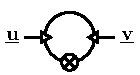
\includegraphics{frg/diagrams/FRG-wetterichEq-FS2_332_1.pdf}\end{gathered} + \subEqTagPrime \label{eq:FS2_332_1-diagram}\\
	&\qquad +\cm{\FSc{\FSidxE{u},\FSidxE{v},\FSidxE{u},\FSidxI{a},\FSidxE{v},\FSidxI{a},\FSidxI{c},\FSidxI{c},\FSidxI{e},\FSidxI{e}}}\,\begin{gathered}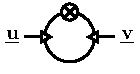
\includegraphics{frg/diagrams/FRG-wetterichEq-FS2_332_2.pdf}\end{gathered} - \subEqTagPrime \label{eq:FS2_332_2-diagram}\\
	&\qquad -\cm{\FSc{\FSidxE{u},\FSidxI{a},\FSidxE{v},\FSidxI{a},\FSidxI{c},\FSidxI{c}}}\,\begin{gathered}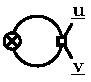
\includegraphics{frg/diagrams/FRG-wetterichEq-FS2_241_1.pdf}\end{gathered}\,. \subEqTagPrime \label{eq:FS2_241_1-diagram}
\end{align}
Computing flow equations for higher-order \nptFunctions{} beyond $n=2$ is in principle straight forward, but the number of involved diagrams grows rapidly making a computation by hand error prone and at some point simply unfeasible.
Packages like \textit{DoFun}~\cite{Huber:2019dkb,DoFun:GitHub} or \textit{QMeS-Derivation}~\cite{Pawlowski:2021tkk,QMeS:GitHub} can be used to automate this process using the computer algebra system \WAMwR.
We use our own \WAM{} code~\cite{Steil:2023PhDFlowEquationsNB} for such and related diagrammatic computations.
The expressions and diagrams in \cref{eq:FS1,eq:FS2,eq:FS3,eq:FS4} have been programmatically generated with our \WAM{} code~\cite{Steil:2023PhDFlowEquationsNB} and exported to \LaTeX{} using propose build export methods.
The diagrams have been programmatically generated and rendered using \textit{Axodraw Version 2}~\cite{Collins:2016aya}.
In the following \cref{eq:FS3,eq:FS4} we present the flow equations for the three- and four-point functions in a skeletonized form\footnote{%
	Following the convention introduced in \cref{sec:compactNotations} we use $\skeleton{n}$ to represent a sequence of $n$ omitted elements.
	$\FScSkeleton{}{n}{}$ are abbreviated \fs{} sign factors, see \cref{eq:FScDef,eq:FScAbr} and the related discussion in \cref{app:FS}.
	$\skeleton{T_{n,k}}$ represents the number of diagrams of a specific type, see \cref{tab:FScombinatorics} and the related discussion.
	
} presenting mainly the classes of involved diagrams.
The flow of the three-point function is governed by
\begin{align}
	\cm{2,\FSvertexDt{\FSidxE{w},\FSidxE{v},\FSidxE{u}}}
	%*** Combinatorics
	&=\, \skeleton{T_{3,3}} + \skeleton{T_{3,2}} + \skeleton{T_{3,1}}\,=\, \skeleton{6} + \skeleton{6} + \skeleton{1} \label{eq:FS3}
	%*** FS expressions
	\newSubEqBlock\\[.25em]
	%FRG`wetterichEq`FS3[{4, {3, 3}}][[1]]
	&= -\cm{\FScSkeleton{}{6}{},\ncm{\FSpropagator{\FSidxI{a},\FSidxI{b}},\FSvertex{\FSidxI{b},\FSidxE{w},\FSidxI{c}},\FSpropagator{\FSidxI{c},\FSidxI{d}},\FSvertex{\FSidxI{d},\FSidxE{v},\FSidxI{e}},\FSpropagator{\FSidxI{e},\FSidxI{f}},\FSvertex{\FSidxI{f},\FSidxE{u},\FSidxI{g}},\FSpropagator{\FSidxI{g},\FSidxI{h}},\FSregulatorDt{\FSidxI{h},\FSidxI{a}}}}+\skeleton{5} +  \subEqTag \label{eq:FS3_433_1}\\[.25em]
	%FRG`wetterichEq`FS3[{3, {3, 1}, {4, 1}}][[1]]
	&\qquad + \cm{\FScSkeleton{}{5}{},\ncm{\FSpropagator{\FSidxI{a},\FSidxI{b}},\FSvertex{\FSidxI{b},\FSidxE{w},\FSidxI{c}},\FSpropagator{\FSidxI{c},\FSidxI{d}},\FSvertex{\FSidxI{d},\FSidxE{v},\FSidxE{u},\FSidxI{e}},\FSpropagator{\FSidxI{e},\FSidxI{f}},\FSregulatorDt{\FSidxI{f},\FSidxI{a}}}}+\skeleton{5} - \subEqTag \label{eq:FS3_33141_1}\\[.25em]
	%FRG`wetterichEq`FS3[{2, {5, 1}}][[1]]
	&\qquad -\cm{\FScSkeleton{}{4}{},\ncm{\FSpropagator{\FSidxI{a},\FSidxI{b}},\FSvertex{\FSidxI{b},\FSidxE{w},\FSidxE{v},\FSidxE{u},\FSidxI{c}},\FSpropagator{\FSidxI{c},\FSidxI{d}},\FSregulatorDt{\FSidxI{d},\FSidxI{a}}}} \subEqTag \label{eq:FS3_251_1}
	\newSubEqBlockPrime\\[.25em]
	%*** Diagrams
	&=-\cm{\FScSkeleton{}{6}{}}\,\begin{gathered}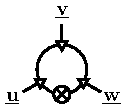
\includegraphics{frg/diagrams/FRG-wetterichEq-FS3_433_1.pdf}\end{gathered}+\skeleton{5} + \subEqTagPrime \label{eq:FS3_433_1-diagram}\\
	&\qquad +\cm{\FScSkeleton{}{5}{}}\,\begin{gathered}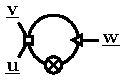
\includegraphics{frg/diagrams/FRG-wetterichEq-FS3_33141_1.pdf}\end{gathered}+\skeleton{5} - \subEqTagPrime \label{eq:FS3_33141_1-diagram}\\
	&\qquad -\cm{\FScSkeleton{}{4}{}}\,\begin{gathered}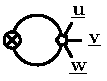
\includegraphics{frg/diagrams/FRG-wetterichEq-FS3_251_1.pdf}\end{gathered}\,, \subEqTagPrime \label{eq:FS3_251_1-diagram}
\end{align}
and the flow of the four-point function follows as
\begin{align}
	\cm{2,\FSvertexDt{\FSidxE{x},\FSidxE{w},\FSidxE{v},\FSidxE{u}}}
	%*** Combinatorics
	&=\, \skeleton{T_{4,4}} + \skeleton{T_{4,3}} + (\skeleton{T_{4,2}}) + \skeleton{T_{4,1}} \,= \notag\\
	&=\, \skeleton{24} + \skeleton{36} + (\skeleton{8} + \skeleton{6}) + \skeleton{1}\label{eq:FS4}
	%*** FS expressions
	\newSubEqBlock\\[.25em]
	%FRG`wetterichEq`FS4[{5, {3, 4}}][[1]]
	&= \cm{\FScSkeleton{}{8}{},\ncm{\FSpropagator{\FSidxI{a},\FSidxI{b}},\FSvertex{\FSidxI{b},\FSidxE{x},\FSidxI{c}},\FSpropagator{\FSidxI{c},\FSidxI{d}},\FSvertex{\FSidxI{d},\FSidxE{w},\FSidxI{e}},\FSpropagator{\FSidxI{e},\FSidxI{f}},\FSvertex{\FSidxI{f},\FSidxE{v},\FSidxI{g}},\FSpropagator{\FSidxI{g},\FSidxI{h}},\FSvertex{\FSidxI{h},\FSidxE{u},\FSidxI{i}},\FSpropagator{\FSidxI{i},\FSidxI{j}},\FSregulatorDt{\FSidxI{j},\FSidxI{a}}}}+\skeleton{23} -  \subEqTag \label{eq:FS4_534_1}\\[.25em]
	%FRG`wetterichEq`FS4[{4, {3, 2}, {4, 1}}][[1]]
	&\qquad -\cm{\FScSkeleton{}{7}{},\ncm{\FSpropagator{\FSidxI{a},\FSidxI{b}},\FSvertex{\FSidxI{b},\FSidxE{x},\FSidxI{c}},\FSpropagator{\FSidxI{c},\FSidxI{d}},\FSvertex{\FSidxI{d},\FSidxE{w},\FSidxI{e}},\FSpropagator{\FSidxI{e},\FSidxI{f}},\FSvertex{\FSidxI{f},\FSidxE{v},\FSidxE{u},\FSidxI{g}},\FSpropagator{\FSidxI{g},\FSidxI{h}},\FSregulatorDt{\FSidxI{h},\FSidxI{a}}}}+\skeleton{35} + \subEqTag \label{eq:FS4_43241_1}\\[.25em]
	%FRG`wetterichEq`FS4[{3, {3, 1}, {5, 1}}][[1]]
	&\qquad + \Big(\cm{\FScSkeleton{}{6}{},\ncm{\FSpropagator{\FSidxI{a},\FSidxI{b}},\FSvertex{\FSidxI{b},\FSidxE{x},\FSidxI{c}},\FSpropagator{\FSidxI{c},\FSidxI{d}},\FSvertex{\FSidxI{d},\FSidxE{w},\FSidxE{v},\FSidxE{u},\FSidxI{e}},\FSpropagator{\FSidxI{e},\FSidxI{f}},\FSregulatorDt{\FSidxI{f},\FSidxI{a}}}}+\skeleton{7} + \subEqTag \label{eq:FS4_33151_1}\\[.25em]
	%FRG`wetterichEq`FS4[{3, {4, 2}}][[1]]
	&\qquad\qquad\quad + \cm{\FScSkeleton{}{6}{},\ncm{\FSpropagator{\FSidxI{a},\FSidxI{b}},\FSvertex{\FSidxI{b},\FSidxE{x},\FSidxE{w},\FSidxI{c}},\FSpropagator{\FSidxI{c},\FSidxI{d}},\FSvertex{\FSidxI{d},\FSidxE{v},\FSidxE{u},\FSidxI{e}},\FSpropagator{\FSidxI{e},\FSidxI{f}},\FSregulatorDt{\FSidxI{f},\FSidxI{a}}}}+\skeleton{5}\Big) - \subEqTag \label{eq:FS4_342_1}\\[.25em]
	%FRG`wetterichEq`FS4[{2, {6, 1}}][[1]]
	&\qquad -\cm{\FScSkeleton{}{5}{},\ncm{\FSpropagator{\FSidxI{a},\FSidxI{b}},\FSvertex{\FSidxI{b},\FSidxE{x},\FSidxE{w},\FSidxE{v},\FSidxE{u},\FSidxI{c}},\FSpropagator{\FSidxI{c},\FSidxI{d}},\FSregulatorDt{\FSidxI{d},\FSidxI{a}}}} \subEqTag \label{eq:FS4_261_1}
	\newSubEqBlockPrime\\[.25em]
	%*** Diagrams
	&=\cm{\FScSkeleton{}{8}{}}\,\begin{gathered}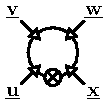
\includegraphics{frg/diagrams/FRG-wetterichEq-FS4_534_1.pdf}\end{gathered}+\skeleton{23} - \subEqTagPrime \label{eq:FS4_534_1-diagram}\\
	&\qquad -\cm{\FScSkeleton{}{7}{}}\,\begin{gathered}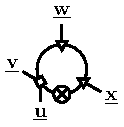
\includegraphics{frg/diagrams/FRG-wetterichEq-FS4_43241_1.pdf}\end{gathered}+\skeleton{35} + \subEqTagPrime \label{eq:FS4_43241_1-diagram}\\
	&\qquad +\Big(\cm{\FScSkeleton{}{6}{}}\,\begin{gathered}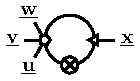
\includegraphics{frg/diagrams/FRG-wetterichEq-FS4_33151_1.pdf}\end{gathered}+\skeleton{7} + \subEqTagPrime \label{eq:FS4_33151_1-diagram}\\
	&\qquad\qquad\quad +\cm{\FScSkeleton{}{6}{}}\,\begin{gathered}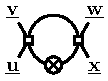
\includegraphics{frg/diagrams/FRG-wetterichEq-FS4_342_1.pdf}\end{gathered}+\skeleton{5}\Big) - \subEqTagPrime \label{eq:FS4_342_1-diagram}\\
	&\qquad -\cm{\FScSkeleton{}{5}{}}\,\begin{gathered}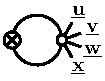
\includegraphics{frg/diagrams/FRG-wetterichEq-FS4_261_1.pdf}\end{gathered}\,. \subEqTagPrime \label{eq:FS4_261_1-diagram}
\end{align}

A common way to reduce the number of diagrams, which only differ by the location of the regulator insertion in the loop, is to introduce the \rgtime{}/scale derivative $\tilde{\partial}_t$ ($\tilde{\partial}_k$) which only acts on the regulator, see, \eg{}, \ccite{DoFun:GitHub}.
This allows for a unification of certain diagrams using
\begin{align}
\tilde{\partial}_t \FSpropagator{\FSidx{a},\FSidx{b}}[\FSmf{\FSsf}] &= - \FSc{\FSidx{b},\FSidx{b}} \FSpropagator{\FSidx{a},\FSidx{m}}[\FSmf{\FSsf}] \FSregulatorDt{\FSidx{m},\FSidx{n}} \FSpropagator{\FSidx{n},\FSidx{b}}[\FSmf{\FSsf}]\, ,
\label{eq:dtTildeG}
\end{align}
which follows directly from the implicit definition \eqref{eq:GkabImplicit} of the propagator.
Using \cref{eq:dtTildeG} to simplify, \ie{}, reduce the number of diagrams, in the flow \cref{eq:FS2,eq:FS3,eq:FS4} requires some care \wrt{} the involved signs and sign factors $(-1)^{\ldots}$. In the following we use $\tilde{\partial}_t$ ($\tilde{\partial}_k$) only for schematic discussions and to simplify final expressions after all traces in field and internal spaces have been performed.

\FloatBarrier%
We conclude this subsection with a remark on the involved combinatorics \dash{} diagrammatic complexity when computing flow equations for higher-order \nptFunctions{} in \fs{}.
The number of diagrams $B_n$ involved on the \rhs{} of a \frg{} flow equation for the \nptFunction{}  ${\protect\FSvertex{\protect\FSidx{x}_1,\ldots,\protect\FSidx{x}_n}}$ grows faster than $n!$.
It is given by the \ith{n} ordered Bell/Fubini number $B_n$~\cite{OEIS:A000670}
\begin{align}
	B_n&= \frac{1}{2}\Phi(\tfrac{1}{2},-n,0) =\sum_{k=1}^{n}T_{n,k} = \frac{1}{2\ln^{n+1}(2)}n!+\order((n-1)!)\, ,\label{eq:FSBn}
\end{align}
where the Triangle numbers $T_{n,k}$~\cite{OEIS:A019538} are given by
\begin{align}
	T_{n,k}&=k! S_n^{(k)}\, ,\label{eq:FSTnk}
\end{align}
with the Hurwitz-Lerch transcendent $\Phi$ and the Stirling number of the second kind $S_n^{(k)}$, see, \eg{}, \ccite{NIST:DLMF} Secs.~25.14 and 26.8.
In a combinatorics context $B_n$ is the ``number of preferential arrangements of $n$ labeled elements; or number of weak orders on n labeled elements; or number of ordered partitions of $[n]$''~\cite{OEIS:A000670}.
For a given $n$ and $k=n,\ldots,1$, $T_{n,k}$ represents the number of diagrams with $k$ vertices, which always have $k+1$ propagators, \cf{} \cref{eq:FS2,eq:FS3,eq:FS4}.
The asymptotic expansion in \cref{eq:FSBn} can be found in \ccite{Barthelemy1980Jan}.
The values of $B_n$ and $T_{n,k}$ for ${k=1,\ldots,n}$ and ${n=1,\ldots,6}$ are displayed in \cref{tab:FScombinatorics}. For further details regarding the underlying combinatorics/permutohedron, see, \eg{}, \ccite{SIMION1997149} p.~167ff and \ccite{Ziegler1995} p.~18ff.
Computing the full flow equations in \fs{} becomes extremely expensive/infeasible for larger $n$.
In this work we mainly study the flow equation for $\FSvertex{}$ itself, with \cref{subsec:0dSU2flowEqs,sec:gnInfInhomo} as the most notable exceptions.
\clearpage
\begin{table}[t]
	\centering
	\caption{\label{tab:FScombinatorics}%
		Number of field space diagrams $B_n$ on the \rhs{} of the flow equation ${\protect\FSvertexDt{\protect\FSidxE{x}_1,\ldots,\protect\FSidxE{x}_n}}$ for ${n=1,\ldots,6}$.
		$T_{n,k}$ diagrams with $k+1$ propagators for ${k=1,\ldots,n}$ contribute to $B_n$ for a given $n$. $B_n$ is given by \cref{eq:FSBn} while $T_{n,k}$ is given by \cref{eq:FSTnk}.
		The factors for $n=2,\ldots,4$ appear in \cref{eq:FS2,eq:FS3,eq:FS4} as $\skeleton{T_{n,k}}$ and $\skeleton{T_{n,k}-1}$ in respective subequations.
	}% Why the protect: [https://tex.stackexchange.com/a/12699/]
	\vspace{\TableAbovecaptionskip}
	\renewcommand{\arraystretch}{1.15}
	\begin{tabular}{l | c  c c c c c || c}
		\toprule
		$T_{n,k} $& $k=1$ & $k=2$ & $k=3$ & $k=4$ & $k=5$ & $k=6$ & $B_n$ \\\midrule
		$n=1$ & $1$ & 	 & 	 & 	 & 	 & 	 & $1$ \\
		$n=2$ & $1$ & $2$ & 	 & 	 & 	 & 	 & $3$ \\
		$n=3$ & $1$ & $6$ & $6$ & 	 & 	 & 	 & $13$ \\
		$n=4$ & $1$ & $14$ & $36$ & $24$ & 	 & 	 & $75$ \\
		$n=5$ & $1$ & $30$ & $150$ & $240$ & $120$ & 	 & $541$ \\
		$n=6$ & $1$ & $62$ & $540$ & $1560$ & $1800$ & $720$ & $4683$ \\
		\bottomrule
	\end{tabular}
\end{table}

\subsection{Renormalization group consistency}\label{subsec:RGconsistency}
In this subsection we discuss the concept of \textit{renormalization group consistency} with focus on the \frg{} framework following the excellent discussion of \ccite{Braun:2018svj}.
Additional information can be found in \ccite{Braun:2003ii,Herbst:2013ufa,Springer2017,Leonhardt:2019mpy,PhysRevD.87.076004}.
In the context of the \frg{} the question of \rgcy{} is closely related to the appropriate choice of \uv{} initial scale $\Lambda$ and corresponding initial action $S_\Lambda$, \cf{} \cref{subsubsec:regulator}.
For a given theory with classical action $S$ the \frg{} provides both a renormalization and regularization scheme based on the \eaa{} $\FSeaa_k$.
The Wetterich equation can be used to study the \rgscale{} evolution of the \eaa{} $\FSeaa_k$ connecting the microscopic action $S$ of the theory at hand to the full quantum \ea{} $\Gamma_\mathrm{1PI}$. 
This process however requires an initialization of the Wetterich equation at an \uv{} initial scale $\Lambda$.
The introduction of such a scale and corresponding regularization, which the regulator provides in the \eaa{} $\FSeaa_k$, is a computational necessity.
Physical observables encoded in $\FSeaa_0[\FSsf]=\Gamma_\mathrm{1PI}[\FSsf]\equiv\Gamma[\FSsf]$ and its moments however should not depend on the scale $\Lambda$:
\begin{align}
	\Lambda\dod{\Gamma[\FSsf]}{\Lambda}\equiv \Lambda\dod{\FSeaa_0[\FSsf]}{\Lambda}\overset{!}{=} 0\,.
	\label{eq:rgcCondition}
\end{align}
This seemingly simple requirement is the governing equation for a consistent regularization and renormalization of a given theory~\cite{Braun:2018svj}.
\Cref{eq:rgcCondition} is called \textit{RG consistency condition} and a computation of $\Gamma[\FSsf]$ for a given theory is considered \textit{RG-consistent} \ifandonlyif{} the condition \nolinebreak[3]\eqref{eq:rgcCondition} is met.
In the \frg{} framework we can translate this requirement for the \ir{} \eaa{} $\FSeaa_0[\FSsf]$ to non-zero $k$ by integrating the \frgEquation{} from the \uv{} $k=\Lambda$ down to $k<\Lambda$\footnote{%
	Due to our convention \eqref{eq:def_rg_time} for \rgtime{}, \cref{eq:rgcWetterichEqInt} and subsequent expressions differ from the corresponding ones in \ccite{Braun:2018svj}, see, \eg{}, Eq. (11a) of \ccite{Braun:2018svj}, involving the \frg{} flux $\FRGflow_{k}[\FSsf]$ by a sign.%
}
\begin{align}
	\FSeaa_k[\FSsf]&= \FSeaa_\Lambda[\FSsf] -\int_\Lambda^k \frac{\dif k'}{k'} \FRGflow_{k'}[\FSsf]\,.
	\label{eq:rgcWetterichEqInt}
\end{align}
By taking a derivative of \cref{eq:rgcWetterichEqInt} \wrt{} $\Lambda$ and evaluating the subsequent expression at ${k=0}$ and an arbitrary ${k\neq\Lambda}$ we obtain
\begin{subequations}\label{eq:rgc}
\begin{align}
	\Lambda\dod{\FSeaa_0[\FSsf]}{\Lambda}&=\Lambda\dod{\FSeaa_\Lambda[\FSsf]}{\Lambda}+\FRGflow_{\Lambda}[\FSsf]\label{eq:rgc0}\,,\\
	\Lambda\dod{\FSeaa_k[\FSsf]}{\Lambda}&=\Lambda\dod{\FSeaa_\Lambda[\FSsf]}{\Lambda}+\FRGflow_{\Lambda}[\FSsf]\label{eq:rgck}\,.
\end{align}
\end{subequations}
Using the \rgcy{} condition \eqref{eq:rgcCondition} with \cref{eq:rgc0} and equating it with \cref{eq:rgck}, we obtain a \rgcy{} condition for any $k\neq \Lambda$
\begin{align}
	0\overset{!}{=} \Lambda\dod{\FSeaa_0[\FSsf]}{\Lambda} =\Lambda\dod{\FSeaa_\Lambda[\FSsf]}{\Lambda}+\FRGflow_{\Lambda}[\FSsf]= \Lambda\dod{\FSeaa_k[\FSsf]}{\Lambda}\, .
	\label{eq:rgcConditionUV}
\end{align}
The included statement $0=\Lambda\partial_\Lambda\FSeaa_\Lambda[\FSsf]+\FRGflow_{\Lambda}[\FSsf]$ in \cref{eq:rgcConditionUV} dictates that \rgcy{} is realized in the \frg{} approach if the \ic{}
$\FSeaa_\Lambda[\FSsf]$ changes with $\Lambda$ according to the \frg{} flux $\FRGflow_{\Lambda}[\FSsf]$ at the initial scale.
The latter is an immensely powerful and practically useful statement and merits further elaboration.

\subsubsection{Construction of RG consistent initial conditions}\label{subsubsec:rgcICS}
Lets first consider a scenario where $\Lambda$ can be chosen asymptotically large in the sense that
\begin{align}
	\forall s_i\in s \quad \frac{s_i}{\Lambda}\ll 1\, ,\label{eq:rgcScales}
\end{align}
with the set $s$ which includes all mass scales of the theory at hand.
This set consists of all intrinsic mass scales $m_\phys$, \eg{}, particle masses and decay widths, and external scales $m_\ext$, \eg{}, temperature $T$ or chemical potential $\mu$.
If $\Lambda$ is indeed asymptotically large compared to those scales, the initial action $\FSeaa_\Lambda[\FSsf]=S[\FSsf]$ can be considered classical in the sense that the \frg{} flux $\FRGflow_{\Lambda}[\FSsf]$ at the initial scale vanishes since all fluctuations are included in $\FSeaa_\Lambda[\FSsf]$.
This entails initial-scale-independence of the \ic{} $\Lambda\partial_\Lambda\FSeaa_\Lambda[\FSsf]=\Lambda\partial_\Lambda S[\FSsf]=0$.
Such situations with asymptotically large initial scale in the sense of \cref{eq:rgcScales} will be studied in \cref{chap:zeroONSU2,chap:GN}.\bigskip

\fullWidthFigure%
	{frg/figures/rg_consistency.pdf}% Graphics
	[]% Sublabels
	{%
		Schematic \frg{} flow \dash{} \rgscaleevolution{} of the \eaa{} in the space of its couplings $\{\lambda_i\}$ \dash{} (in blue and red) from the \uv{} initial condition $\FSeaa_\Lambda$ towards the \ir{} at differing external parameter sets $m_\ext^{(0)}\neq m_\ext^{(1)}$.
		The red-dashed line represents a \rg{} inconsistent flow at $m_\ext^{(1)}$ starting from $\FSeaa_{\Lambda'}^{(0)}$ and not ending at the correct \ir{} result $\FSeaa_{0}^{(1)}$.
		For readability in the figure we abbreviated $\FSeaa_k^{(0)}\equiv\FSeaa_k[\FSsf;m_\ext^0]$ and $\FSeaa_k^{(1)}\equiv\FSeaa_k[\FSsf;m_\ext^1]$.%
	}%Caption
	{fig:frg_rg_consistency}%Label
In certain applications \dash{} prominently when working with \loefts{} of \qcd{}, \cf{} \cref{sec:qcdModels,chap:QMM} \dash{} choosing an asymptotically large $\Lambda$ for a given classical action $S$ is conceptually not feasible and in some cases even mathematically impossible.
In those cases it is possible to use \rgcy{} as a construction principle for a \rgscaledependent{} \ic{} $\FSeaa_\Lambda[\FSsf]=S_\Lambda[\FSsf]$ in the following way.

Consider a \loeft{} for which we specify the action ${\FSeaa_\LambdaP[\FSsf;m_\ext^0]=S[\FSsf]}$ at an intermediate scale $\LambdaP$ with/at a corresponding set of physical parameters $m_\phys^0$/ external scales $m_\ext^0$.
Here $m_\ext^0$ is typically (but not necessarily) the vacuum, \eg{}, $T=\mu=0$, and  $m_\phys^0$ a set of \ir{} observables realized by properly chosen couplings in $\FSeaa_\LambdaP[\FSsf]$.
In this scenario $\LambdaP$ can not be considered as asymptotically large in the sense of \cref{eq:rgcScales} and thus $\FSeaa_\LambdaP[\FSsf]$ does not include all relevant fluctuations especially \wrt{} fluctuations related to external scales $m_\ext$ beyond $m_\ext^0$, \eg{}, thermal and density fluctuations beyond the vacuum.
$\FSeaa_\LambdaP[\FSsf;m_\ext^0]$ is therefore not suited for computations at $m_\ext^1\neq m_\ext^0$.
To remedy these situations and to enable \rgct{} computations at differing external scales $m_\ext^1\neq m_\ext^0$ one can use the Wetterich equation~\eqref{eq:rgcWetterichEqInt} to reconstruct an \uv{} initial action $\FSeaa_\Lambda[\FSsf;m_\ext^0]$ at a higher, proper \uv{} initial scale $\Lambda>\LambdaP$:
\begin{align}
	S_\Lambda[\FSsf]\equiv\FSeaa_\Lambda[\FSsf;m_\ext^0]&= \FSeaa_\LambdaP[\FSsf;m_\ext^0] +\int_\Lambda^\LambdaP \frac{\dif k'}{k'} \FRGflow_{k'}[\FSsf;m_\ext^0]\,.
	\label{eq:rgcEq14}
\end{align}
$S_\Lambda[\FSsf]$ includes \rgscaledependent{} counter terms \dash{} corrections to $S[\FSsf]$ \dash{} generated by the \frg{} flux $\FRGflow_{k}[\FSsf;m_\ext^0]$ to ensure \rgcy{} $\Lambda\partial_\Lambda\FSeaa_0[\FSsf]=0$ by guaranteeing $\Lambda\partial_\Lambda \FSeaa_\Lambda[\FSsf;m_\ext^0] = -\FRGflow_{\Lambda}[\FSsf;m_\ext^0]$ while maintaining $\FSeaa_\LambdaP[\FSsf;m_\ext^0]=S[\FSsf]$. 
Therefore guaranteeing an unchanged $\FSeaa_k[\FSsf;m_\ext^0]$ for $k<\LambdaP$ by construction, since \cref{eq:rgcWetterichEqInt} at $m_\ext^0$ and \cref{eq:rgcEq14} entail
\begin{subequations}\label{eq:rgcEq15}
\begin{align}
	\FSeaa_k[\FSsf;m_\ext^0]&= \FSeaa_\LambdaP[\FSsf;m_\ext^0] -\int_\LambdaP^k \frac{\dif k'}{k'} \FRGflow_{k'}[\FSsf;m_\ext^0]\label{eq:rgcEq15a}\\
	&=\FSeaa_\Lambda[\FSsf;m_\ext^0] -\int_\Lambda^k \frac{\dif k'}{k'} \FRGflow_{k'}[\FSsf;m_\ext^0]\label{eq:rgcEq15n}\, .
\end{align}
\end{subequations}
$S_\Lambda[\FSsf]$ represents an \uv{} completion of the \loeft{} specified at $\LambdaP$ with ${\FSeaa_\LambdaP[\FSsf;m_\ext^0]=S[\FSsf]}$.
This construction is visualized in \cref{fig:frg_rg_consistency} in blue.

By reconstructing $S_\Lambda[\FSsf]\equiv\FSeaa_\Lambda[\FSsf;m_\ext^0]$ up to a scale $\Lambda$, which can be considered as asymptotically large in the sense of \cref{eq:rgcScales}, we can ensure that a change in external parameters leaves the regularization and renormalization encoded in the running of $S_\Lambda[\FSsf]$ unchanged:
\begin{align}
	\dod{}{m_\ext}\!\sbr{\Lambda\dod{S_\Lambda[\FSsf]}{\Lambda}}=0\,.
	\label{eq:rgcEq3} 
\end{align}
In other words $S_\Lambda[\FSsf]$ is suited for computations at $m_\ext^1\neq m_\ext^0$ since $\Lambda\gg m_\ext$ and $\FRGflow_{\Lambda}[\FSsf;m_\ext^0]=\FRGflow_{\Lambda}[\FSsf;m_\ext^1]$.
Integrating \cref{eq:rgcEq3} from $m_\ext^0$ to $m_\ext^1$ we obtain
\begin{align}
	\Lambda\dod{S_\Lambda[\FSsf]}{\Lambda} \equiv \Lambda\dod{\FSeaa_\Lambda[\FSsf;m_\ext^0]}{\Lambda} = \Lambda\dod{\FSeaa_\Lambda[\FSsf;m_\ext^1]}{\Lambda}\,.
	\label{eq:rgcEq3int}
\end{align}
Note that $\FSeaa_\Lambda[\FSsf;m_\ext^1]=\FSeaa_\Lambda[\FSsf;m_\ext^0]$ is not necessary: an explicit dependence of $S_\Lambda[\FSsf]$ on $m_\ext$ is possible\footnote{
	Certain \loefts{} can require counter terms in $S_\Lambda[\FSsf]$, which depend on $m_\ext$ explicitly, see, \eg{}, Sec.~III.B of \nbccite{Braun:2018svj} for an explicit example involving diquarks and chemical potential in the context of \loefts{} for \qcd{}.%
} as long as \cref{eq:rgcEq3int} holds.
In \cref{fig:frg_rg_consistency} and our applications in \cref{chap:QMM} we consider $S_\Lambda[\FSsf]$ without an explicit dependence on $m_\ext$.
Using the Wetterich equation \eqref{eq:rgcWetterichEqInt} at $m_\ext^1$ with \cref{eq:rgcEq14}, we can construct a \rgcy{} condition at $m_\ext^1\neq m_\ext^0$:
\begin{subequations}\label{eq:rgcm}
\begin{align}
	0&\overset{!}{=} \Lambda\dod{\FSeaa_0[\FSsf;m_\ext^1]}{\Lambda} =\Lambda\dod{\FSeaa_k[\FSsf;m_\ext^1]}{\Lambda}= \Lambda\dod{\FSeaa_\Lambda[\FSsf;m_\ext^1]}{\Lambda} + \FRGflow_{\Lambda}[\FSsf;m_\ext^1]\, ,\label{eq:rgcm1p}\\
	0&\overset{!}{=}\Lambda\dod{\FSeaa_0[\FSsf;m_\ext^1]}{\Lambda} = \FRGflow_{\Lambda}[\FSsf;m_\ext^1]-\FRGflow_{\Lambda}[\FSsf;m_\ext^0]\label{eq:rgcm1}\, ,
\end{align}
\end{subequations}
where we used \cref{eq:rgcEq3int} in \cref{eq:rgcm1p} to obtain \cref{eq:rgcm1}.
The latter can be used to conveniently define applicability ranges $\Lambda[m_\ext^1]$, where $\Lambda[m_\ext^1]$ is the range/scale for which \cref{eq:rgcm1} holds to a given accuracy~\cite{Braun:2018svj}.
Using $S_\Lambda[\FSsf]$ as an \ic{} for a large range of external parameters $m_\ext$ by guaranteeing \cref{eq:rgcm1} (to a chosen accuracy), we note that at $k=\LambdaP$
\begin{align}
	\FSeaa_\LambdaP[\FSsf;m_\ext^1]&= \FSeaa_\LambdaP[\FSsf;m_\ext^0] -\int_\Lambda^\LambdaP \frac{\dif k'}{k'} \del{\FRGflow_{k'}[\FSsf;m_\ext^1]-\FRGflow_{k'}[\FSsf;m_\ext^0]}\,,
	\label{eq:rgcSLambdaPmext1}
\end{align}
where we again used the Wetterich equation \eqref{eq:rgcWetterichEqInt} with \cref{eq:rgcEq14}.
$\FSeaa_\LambdaP[\FSsf;m_\ext^1]$ differs from the specified action $\FSeaa_\LambdaP[\FSsf;m_\ext^0]=S[\FSsf]$ by the fluctuations associated with $m_\ext$.
The latter are incorporated by integrating the difference of \frg{} fluxes $\FRGflow_{k'}[\FSsf;m_\ext^1]-\FRGflow_{k'}[\FSsf;m_\ext^0]$ from $\Lambda$ to $\LambdaP$, \cf{} \cref{fig:frg_rg_consistency}.
It is imperative to include those fluctuations at $k=\LambdaP$ and $\FSeaa_\LambdaP[\FSsf;m_\ext^0]=S[\FSsf]$ alone is not suited for a flow at $m_\ext^1$ \dash{} a situation illustrated in \cref{fig:frg_rg_consistency} in red.\bigskip

To conclude this section we want to comment on some practical limitations when leveraging the concept of \rgcy{}.
Throughout this section we frequently used the symbolically integrated Wetterich equation \eqref{eq:rgcWetterichEqInt} which is not a simple equation involving an ordinary integral.
The integrals in \cref{eq:rgcWetterichEqInt} and subsequent derived expressions are meant as solutions of the Wetterich equation, which are obtained by solving the differential equations associated with the \frg{} flux $\FRGflow_{k}[\FSsf]$.
Depending on the theory and truncation at hand this might be a rather involved process.
Furthermore \frg{} time integration \dash{} evolving the Wetterich equation in \rgscale{} from the \uv{} to the \ir{} \dash{} is for many theories and truncations irreversible.
This irreversibility is formally mentioned in the next \cref{subsec:RGflow} and discussed at length in \cref{chap:zeroONSU2} and especially in \cref{subsec:0dO1Entropy}.
Irreversibility makes the construction \eqref{eq:rgcEq14} of $S_\Lambda[\FSsf]\equiv\FSeaa_\Lambda[\FSsf;m_\ext^0]$ in the context of \loefts{} rather involved since a solution from the lower scale $\LambdaP$ up to $\Lambda>\LambdaP$ is practically/computationally not possible and
\begin{align}
	\FSeaa_\Lambda[\FSsf;m_\ext^0]-\int_\Lambda^\LambdaP \frac{\dif k'}{k'} \FRGflow_{k'}[\FSsf;m_\ext^0] &= \FSeaa_\LambdaP[\FSsf;m_\ext^0]\,
	\label{eq:rgcEq14rev}
\end{align}
would be the practical form of \eqref{eq:rgcEq14}:
$\FSeaa_\Lambda[\FSsf;m_\ext^0]$ has to be tuned such that $\FSeaa_\LambdaP[\FSsf;m_\ext^0]$ is recovered after flowing down from $\Lambda$ to $\LambdaP$. 
This presents an extremely difficult optimization problem, which might not even have (depending on the theory, truncation, and regulator employed) a solution for some explicit choices of $\FSeaa_\LambdaP[\FSsf;m_\ext^0]\equiv S[\FSsf]$.

That being said for some theories and truncations \frg{} time integration is reversible, \cf{} our large-$N$/mean-field studies in \cref{chap:GN,chap:QMM}, which simplifies the construction of suitable initial conditions $S_\Lambda[\FSsf]\equiv\FSeaa_\Lambda[\FSsf;m_\ext^0]$ immensely since direct computation of appropriate counter terms from the \cref{eq:rgcEq14} is possible and an optimization/tuning in the sense of \cref{eq:rgcEq14rev} is not required.

\subsection{Renormalization group equations as functional flow equations}\label{subsec:RGflow}
\begin{disclaimer}
	Parts of this subsection are based on the Secs.~II.B\dash{}C and IV.A of \nbccite{Koenigstein:2021syz}.
\end{disclaimer}
In the following we want to comment on the structure of the renormalization group equation for the \rgscaledependent{} generating functionals $Z_k[\FSff{J}]$, $W_k[\FSff{J}]$, and $\FSeaa_k[\FSmf{\FSsf}]$ for non-composite/non-scale-dependent fundamental fields $\FSfd{\FSsf}{a}\equiv\FSffd{\FSsf}{a}\Leftrightarrow \partial_t \FSfd{\FSsf}{a}=0$ and corresponding sources $\FSfd{J}{a}\equiv\FSffd{J}{a}$.
The evolution equation \eqref{eq:dWkdt} simplifies in this context to 
\begin{align}
	\dod{W_k[\FSff{J}]}{t}&=\dod{}{t}\ln Z_k[\FSff{J}]=\frac{1}{Z_k[\FSf{J}]}\dod{Z_k[\FSf{J}]}{t}
	= -\frac{1}{2}\partial_t \FSregulator{\FSidx{m},\FSidx{n}}\expectationValue{\FSffd{\FSsf}{n}\FSffd{\FSsf}{m}}{\FSff{J}}
	\label{eq:dWkdtnoscale}\,,
\end{align}
from which we can deduce the following evolution equations 
\begin{align}
	\dod{Z_k[\FSff{J}]}{t}&= -\frac{1}{2}\del{\partial_t \FSregulator{\FSidx{m},\FSidx{n}}}\frac{\delta}{\delta \FSmfu{J}{n}}\frac{\delta}{\delta \FSmfu{J}{m}} Z_{k}[\FSff{J}]
	= -\frac{1}{2}\del{\partial_t \FSregulator{\FSidx{m},\FSidx{n}}} Z_{k,\FSidx{n}\FSidx{m}}[\FSff{J}]\label{eq:dZkdtflow}\,,\\
	\dod{W_k[\FSff{J}]}{t}&= -\frac{1}{2}\del{\partial_t \FSregulator{\FSidx{m},\FSidx{n}}}\del[3]{ \frac{\delta}{\delta \FSmfu{J}{n}}\frac{\delta}{\delta \FSmfu{J}{m}} W_{k}[\FSff{J}] + \frac{\delta W_{k}[\FSff{J}]}{\delta \FSmfu{J}{n}}\frac{\delta W_{k}[\FSff{J}]}{\delta \FSmfu{J}{m}} }=\notag\\
	&= -\frac{1}{2}\del{\partial_t \FSregulator{\FSidx{m},\FSidx{n}}} \del[3]{W_{k,\FSidx{n}\FSidx{m}}[\FSff{J}]+W_{k,\FSidx{n}}[\FSff{J}]W_{k,\FSidx{m}}[\FSff{J}]}
	\label{eq:dWkdtflow}\,,
\end{align}
by rewriting the expectation value using the generating functionals.
The structure of \cref{eq:dZkdtflow} is that of a linear functional diffusion equation (\textit{heat equation})~\cite{Brydges:1987,Zumbach:1994kc,Rosten:2010vm,SkinnerScript,Salmhofer:2020Talk,Cannon:1984}, where $t$ corresponds to an effective temporal direction, while $\FSff{J}$ corresponds to an effective spatial direction.
Sometimes \cref{eq:dZkdtflow} is even explicitly denoted as a (non-linear) heat equation, \cf{} \cref{paragraph:HE}.
The regulator insertion $-\frac{1}{2}\partial_t \FSregulator{\FSidx{m},\FSidx{n}}$ acts as a diffusion coefficient contracted with the Hessian $Z_{k,\FSidx{n}\FSidx{m}}[\FSff{J}]$.
The \rgtime{} evolution of the generating functional $Z_k[\FSff{J}]$ is governed by the change \dash{} functional derivative $\delta/\delta{\FSffd{J}{n}}$ \dash{} of the functional gradient $Z_{k,\FSidx{m}}[\FSff{J}]$ weighted by the diffusion coefficient $-\frac{1}{2}\partial_t \FSregulator{\FSidx{m},\FSidx{n}}$.
The closely related evolution equation \eqref{eq:dWkdtflow} for $W_k[\FSff{J}]$ has a similar structure, but the Hessian $W_{k,\FSidx{n}\FSidx{m}}[\FSff{J}]$ gets modified by the product of two functional gradient terms $W_{k,\FSidx{n}}[\FSff{J}]W_{k,\FSidx{m}}[\FSff{J}]$.
The evolution equations for $Z_k[\FSff{J}]$ and $W_k[\FSff{J}]$ are due to their nature as functional diffusion equations \textit{flow equations}.

The \frgEquation{} 
\begin{align}
	\partial_t\FSeaa_k[\FSsf]
	%FRG`wetterichEq`FS0[{1}][[1]]
	=\frac{1}{2}\ncm{\FSpropagator{\FSidx{m},\FSidx{n}}[\FSsf],\FSregulatorDt{\FSidx{n},\FSidx{m}}}
	\equiv \FRGflow_k\sbr[1]{\mkern2mu\FSvertex{\FSidx{m},\FSidx{n}}[\FSmf{\FSsf}],\FSsf}\,,\label{eq:WetterichEqFlow}
\end{align}
does not manifest itself as a diffusion or flow equation at first glance. 
The \rhs{} of \cref{eq:WetterichEqFlow} depends non-linearly on the Hessian $\FSvertex{\FSidx{m},\FSidx{n}}[\FSmf{\FSsf}]$ through the propagator, \cf{} \cref{eq:GkabImplicit}, which prevents a direct interpretation as a linear functional diffusion equation.
Noting however that the \rhs{} of \cref{eq:WetterichEqFlow} does not depend on $\FSeaa_k[\FSsf]$ itself, we may consider the functional gradient $\FSvertex{\FSidx{a}}[\FSmf{\FSsf}]$ as the fundamental variable and by taking a corresponding functional derivative reformulate \cref{eq:WetterichEqFlow} as
\begin{align}
	\partial_t \FSvertex{\FSidx{a}}[\FSmf{\FSsf}] = \frac{\delta}{\delta \FSmfd{\FSsf}{a}}\FRGflow_k\sbr[1]{\mkern2mu\FSvertex{\FSidx{m},\FSidx{n}}[\FSmf{\FSsf}],\FSsf}\equiv\FRGflow_k^{,\FSidx{a}}\sbr[1]{\mkern2mu\FSvertex{\FSidx{m},\FSidx{n}}[\FSmf{\FSsf}],\FSsf}\,,
	\label{eq:dWetterichEqFlow}
\end{align}
which has the form of a functional convection\footnote{
	In the following we use the term \textit{convection} in the fluid-dynamical sense as a phenomenon including both \textit{advection} and \textit{diffusion}.
	For more details on those terms we refer to \cref{sec:conservationLaws}.%
} equation~\cite{Koenigstein:2021syz,Grossi:2019urj}.
The \rgtime{} evolution of the one-point function $\FSvertex{\FSidx{a}}[\FSmf{\FSsf}]$ is governed by the change \dash{} functional derivative $\delta/\delta \FSmfd{\FSsf}{a}$ \dash{} of the convection flux $\FRGflow_k\sbr[1]{\mkern2mu\FSvertex{\FSidx{m},\FSidx{n}}[\FSmf{\FSsf}],\FSsf}$, which due to the non-linear dependence on $\FSvertex{\FSidx{m},\FSidx{n}}[\FSmf{\FSsf}]$ can include both advective and diffusive contributions~\cite{Koenigstein:2021syz,Grossi:2019urj}, \cf{} \cref{subsubsec:exact_flow_equation_potential}.\bigskip

The fact that the non-perturbative \rg{} evolution equations manifest as flow equations in the form of functional convection equations has many interesting and relevant consequences.
We will not go into detail at this point and reserve an in-depth discussion for the main part of this thesis.
The only aspect we want to mention at this point is the fact, that the manifestation as functional convection equations is closely linked to the semigroup property \dash{} the irreversibility of non-perturbative \rg{} steps \dash{} of the \grg{}.
The related loss of micro-physical information in the \grg{} due to the successive integration over high-momentum modes, \cf{} \cref{subsubsec:regulator}, manifests on the level of the evolution \cref{eq:dZkdtflow,eq:dWkdtflow,eq:dWetterichEqFlow} in their nature as convection equations.
Especially the diffusive nature of the equations seems rather intuitive and natural in the context of non-perturbative implementations of the \rg{}.

On the level of the \rgscaledependent{} generating functionals $Z_k[\FSff{J}]$, $W_k[\FSff{J}]$, and $\FSeaa_k[\FSmf{\FSsf}]$, without specifying an explicit theory and truncation, it is difficult to discuss the implications of this formulation and the understanding of \rg{} evolution equations as flow equations explicitly. 
We will do so in the main part of this thesis using zero-dimensional theories in \cref{chap:zeroONSU2} and the \gnm{} in \cref{chap:GN}.
To facilitate this, we discuss flow equations/conservation laws with advective, diffusive, and source terms in the following \cref{sec:conservationLaws}.

\section{Conservation laws, hydrodynamics, and the finite volume method}\label{sec:conservationLaws}
\begin{disclaimer}
	Parts of this section are based on Secs.~IV.B\dash{}C of \nbccite{Koenigstein:2021syz} and on the Apps.~B\dash{}E of \nbccite{Steil:2021cbu}. 
\end{disclaimer}
In this section we discuss systems of \pdes{} in one effective temporal direction $(t)$ and one effective spatial direction $(x)$ of the following generic form
\begin{align}
	&\dift\! u_i ( t, x ) + \difx\!  F_i [ t, x, \{u_i ( t, x )\} ] = \difx\! Q_i [ t, x, \{u_i ( t, x )\}, \{\partial_x u_i ( t, x )\} ]\,+\notag\\*[.2em] % no page break here
	&\hphantom{\dift\! u_i ( t, x ) + \difx\!  F_i [ t, x, \{u_i ( t, x )\} ] = \difx\! Q_i [ t, x, \{u_i ( t, x )\}xxx}+S_i [ t, x, \{u_i ( t, x )\} ] \, , \label{eq:FVadsEq}\\[.2em]
	&\dift\! u_i ( t, x ) + \difx\! C_i [ t, x, \{u_i ( t, x )\}, \{\partial_x u_i ( t, x )\} ] = S_i [ t, x, \{u_i ( t, x )\} ] \, , \label{eq:FVcsEq}
\end{align}
where we distinguish between advective contributions $\difx\! F_i[\ldots]$, diffusive contributions$\difx\! Q_i[\ldots]$, and source/sink contributions $S_i [\ldots]$.
Whether $S_i$ acts as a source or sink in the dynamics of $\{u_i(t,x)\}$ depends on its explicit form.
Nevertheless we will usually refer to $S_i$ as a source term.
We also introduced the convective contribution $\difx\! C_i[\ldots]\equiv \difx\! F_i[\ldots] - \difx\! Q_i[\ldots]$, which incorporates both advective and diffusive contributions for the sake of discussion. 
In this section we will explicitly distinguish between partial $(\partial_x\equiv\partial/\partial x)$ and total  $(\difx\!\equiv\!\dif/\!\dif x)$ derivatives.
In the following, we occasionally suppress the $t$- and $x$-dependencies of $u_i$, $C_i$, $F_i$, $Q_i$, and $S_i$ for the sake of simplicity.
Equation \eqref{eq:FVadsEq} is a system of \pdes{} describing the evolution of $m$ conserved quantities $\{u_i ( t, x )\}\equiv \{u_i\}\equiv\{ u_1 , \ldots , u_m \}$ in $t$ and $x$. 
Depending on the problem at hand these two directions are not necessarily identical with physical spatial and temporal dimensions, but for the following discussion we denote them as such.
The functions 
\begin{itemize}
	\item $F_i [ \{u_i\} ] \equiv F_i [ t, x, \{u_i ( t, x )\} ]$ are components of a non-linear advection flux, 
	\item $ Q_i [ \{u_i\} , \{\partial_x u_i\} ] \equiv Q_i [ t, x, \{u_i ( t, x)\} , \{\partial_x u_i ( t, x )\} ]$ are components of a non-linear diffusion(dissipation) flux, and 
	\item $S_i [ \{u_i\} ] \equiv S_i [ t, x, \{u_i ( t, x)\} ]$ are components of a source term.
\end{itemize}
The aforementioned fluxes are discussed in detail in \cref{subsec:hydroAdvection,subsec:hydroDiffusion,subsec:hydroSource} respectively.
The concepts discussed in the following can be generalized beyond one spatial dimension to \dxyDimensional{s}{1} space-time: $( x, t ) \rightarrow ( \vec{x}, t ) = ( x_1, \ldots, x_d, t )$.
Equation systems similar or even identical to \cref{eq:FVadsEq} are often referred to as conservation laws and appear in many areas of the natural sciences, engineering, and economics.
They are extensively studied in the field of \acrrepeat{cfd}.

A complete and self-contained introduction to conservation laws in the context of \cfd{} is beyond the scope of this thesis.
We rather focus on introducing the computational methods we employ, establishing relevant nomenclature, and discussing selected properties of the system~\eqref{eq:FVadsEq}.
We will discuss the different contributions to \cref{eq:FVadsEq} in \cref{subsec:hydroAdvection,subsec:hydroDiffusion,subsec:hydroSource,subsec:hydroEuler} using explicit educational examples.
The methodological introduction of \cref{subsec:hydroFV,subsec:hydroKT} is meant to facilitate the computations and discussions in the main part of this thesis, \ie{}, \cref{chap:zeroONSU2,chap:GN}.
For more details we refer the interested reader to the vast literature discussing conservation laws, \cf{} \ccite{LeVeque:1992,Eymard2000Jan,LeVeque:2002,Hesthaven2007,RezzollaZanotti:2013,Hunter2014,MishraLectureNotes,Vazquez-Cendon2015,polyanin2016handbook,Rezolla2020}.

This section has a corresponding digital auxiliary file~\cite{Steil:2023PhDFVNB}, which includes our latest \WAM{}-implementation of the \acrshort{kt}/\acrshort{knp} scheme discussed in \cref{subsec:hydroKT} and the code to produce all the explicit (numerical) examples discussed in \cref{subsec:hydroAdvection,subsec:hydroDiffusion,subsec:hydroSource,subsec:hydroEuler}.

\clearpage
\subsection{The finite volume method}\label{subsec:hydroFV}
\begin{disclaimer}
	This subsection follows the discussion in Sec.~IV.B of \nbccite{Koenigstein:2021syz} with slight modifications due to the fact that we want to discuss a system of conservation laws for $\{u_i ( t, x )\}$ instead of a single conservation law for $u ( t, x )$. 
\end{disclaimer}
In this section we discuss a numerical solution scheme for convection/advection-diffusion equations\footnote{%
	Oftentimes, such equations are also referred to as ``convection-diffusion equations''.
	The semantically correct term is nevertheless ``advection-diffusion equation'' because ``convection'' also includes diffusive processes besides the transport by bulk motion (advection), see also \ccite{LeVeque:1992}.%
} 
with source terms of the generic type \eqref{eq:FVcsEq}. 
Considering the convection equation~\eqref{eq:FVcsEq} with specified terms $F_i$, $Q_i$, and $S_i$ in a finite computational domain $\Omega = \mathcal{V} \times [ t_0, t_N ]$, where $\mathcal{V} \subset \Reals{}^1$ denotes the spatial volume, with an \ic{} $u_i( t_0, x )$ and Dirichlet (Neumann) \bcs{} specifying $( \partial_x ) u_i ( t, x ) |_{x \in \partial \mathcal{V}}$, the natural question arises how to evolve the \ic{} in time from $t_0$ to $t_N>t_0$ to acquire a solution $u ( t_N, x )$ respecting the specified \bcs{} \dash{} \ie{}, how to explicitly solve the posed initial-value problem.
For most problems of the type~\eqref{eq:FVcsEq} an analytic/symbolic explicit solution is not known or even considered to be non-existent.
Strategies for finding numerical (weak) solutions are required.
Numerical schemes in the broad class of so-called \acrrepeat{fv} methods are very popular for the numerical solution of \pdes{} describing the conservation or balance of quantities.
For additional details regarding especially the \fv{} method we refer the interested reader to the textbooks~\cite{LeVeque:2002,Vazquez-Cendon2015}.
Alternative \hrsc{} schemes in modern computational fluid dynamics are among others: finite-difference schemes including flux limiters/numerical viscosity or finite-element methods.

The concept that all numerical \fv{} methods share is a discretization of the computational domain into space-time control volumes $\mathcal{V}_j \times [ t^l, t^{l+1} ]$, where the set of spatial control volumes $\mathcal{V}_j$ covers the spatial computational domain $\mathcal{V}$.
Integrating \cref{eq:FVcsEq} over such a control volume centered at $x$, using the divergence theorem (Gauss-Ostrogradsky theorem) on the convection flux, and introducing the sliding cell average
\begin{align}
	\bar{u}_{i} ( t, x ) &\equiv \frac{1}{| \mathcal{V}_j |} \int_{\mathcal{V}_j} \dif\xi \, u_i( \xi, t )\\
	\Rightarrow \bar{u}_{i,j}(t)\equiv \bar{u}_{i} ( t, x_j ) &\equiv \frac{1}{\Delta x_j} \int_{x_{j-\frac{1}{2}}}^{x_{j+\frac{1}{2}}} \dif\xi \, u_i( \xi, t )\, ,\label{eq:FVaverage}
\end{align}
where $\mathcal{V}_j = \{ \xi : | \xi - x_j | \leq \Delta x_j/2 \}$, we arrive at an equivalent integral form of \cref{eq:FVcsEq},
\begin{align}
	\bar{u}_i ( t^{l+1}, x ) = \bar{u}_i ( t^l, x ) - \bar{C}_i[ t^{l+1},t^l, x,\{u_i\} ] + \bar{S}_i[ t^{l+1},t^l, x,\{u_i\} ]\label{eq:FVintEq}\,,
\end{align}
with the integral over the convection flux 
\begin{align}
	\bar{C}_i[ t^{l+1},t^l, x,\{u_i\} ]&\equiv \tfrac{1}{\Delta x_j}\int_{t^l}^{t^{l+1}} \dif\tau \, C_i \big[ \tau, x + \tfrac{\Delta x_j}{2}, u_i \big\{ \big( \tau, x + \tfrac{\Delta x_j}{2} \big) \big\} \big]\, -\notag\\* % no page break
	&\qquad\qquad-\tfrac{1}{\Delta x_j}\int_{t^l}^{t^{l+1}} \dif\tau \, C_i \big[ \tau, x - \tfrac{\Delta x_j}{2},  \big\{u_i \big( \tau, x - \tfrac{\Delta x_j}{2} \big)  \big\}\big]\,,\label{eq:FVcIntEq}
\end{align}
and the integral over the source term
\begin{align}
	\bar{S}_i[ t^{l+1},t^l, x,\{u_i\} ]&\equiv \frac{1}{\Delta x_j}  \int_{t^l}^{t^{l+1}} \dif\tau \int_{x_{j-\frac{1}{2}}}^{x_{j+\frac{1}{2}}} \dif\xi \, S_i [ \tau, \xi, \{u_i ( \tau, \xi )\} ] \,,\label{eq:FVsIntEq}
\end{align}
with $x\in\mathcal{V}_j$.
Considering a system without explicit source terms $(S_i=0)$, \cref{eq:FVintEq} with \cref{eq:FVcIntEq} implies that the change in the cell average $\bar{u}_i ( t^{l+1}, x )-\bar{u} ( t^l, x )$ is given by the time-integral over the convection flux \eqref{eq:FVcIntEq} \dash{} \ie{}, the time-integral over the in- and out-flux at the cell interfaces $x\pm\frac{\Delta x_j}{2}$.
Assuming appropriate closed \bcs{} on the compact spatial volume $\mathcal{V}$, the spatial integral over the cell averages $\bar{u}_{i} ( t, x )$ is conserved since change in the individual control volumes is only possible due to in- or out-flux through the cell interfaces into the neighboring control volumes \dash{} hence the name conservation laws.
In a system with closed \bcs{} changes in the sum/integral over the cell averages $\bar{u}_{i} ( t, x )$ are only possible due to source/sink terms $S_i$, which modify the conservation law according to \cref{eq:FVintEq} with \cref{eq:FVsIntEq}.
The reformulation of \cref{eq:FVcsEq} in terms of cell averages has several advantages which we will discuss in the following.
Arguably the most important one, which we want to mention right away, is the fact, that the integral/weak formulation of \cref{eq:FVintEq} in terms of cell averages allows for a proper treatment of discontinuous solutions $u_{i} ( t, x )$, which are notorious in the context of conservation laws.\bigskip

The solution of \cref{eq:FVintEq} \dash{} \ie{}, the explicit computation of \cref{eq:FVcIntEq,eq:FVsIntEq} \dash{} presents the central challenge for an explicit \fv{} scheme.
Details regarding the explicit resolution and computation of \cref{eq:FVcIntEq,eq:FVsIntEq} are discussed in \cref{subsec:hydroKT} and specifically in \cref{subsec:hydroAdvection,subsec:hydroDiffusion,subsec:hydroSource} respectively.

A central aspect of each practical \fv{} scheme is an appropriate and informed choice of the space-time control volumes, which, depending on the scheme and problem at hand, might change during the time evolution. 
Given a set of control volumes and a corresponding set of cell averages $\bar{u}_i ( t^l, x_j ) \equiv \bar{u}^l_{i,j}$ the time evolution to ${t^{l+1}\equiv t^l+\Delta t}$ requires the solution of the Riemann problems at each cell interface.
A Riemann problem in this \cfd{} context is the \ivp{} related to the time evolution of two initially spatially constant states left and right of an initial interface, see, \eg{}, \ccite{Toro2009,Lax1973,Ames:1992,LeVeque:1992,LeVeque:2002,Hesthaven2007,RezzollaZanotti:2013,Vazquez-Cendon2015} for details.
Part of these problems are the fluxes through the cell boundaries.
The computation of those fluxes requires a reconstruction of the values of $u_i$ on the cell interfaces located at $x_{j + \ttfrac{1}{2}}$, which we denote as $u_{i,j + \ttfrac{1}{2}}^l$, from the given set of cell averages $\bar{u}_{i,j}^l$.
This is usually done by means of a carefully constructed polynomial approximation respecting the given cell averages of the neighboring cells.
The order of the chosen approximation is one of the factors contributing to the overall spatial order (of the error) of the scheme at hand.

Given the cell averages $\bar{u}_{i,j}^l$ and fluxes through the cell interfaces at $t=t^l$ it remains to solve the Riemann problems at each cell interface.
The solution of the Riemann problem amounts to the exact evaluation of the flux integrals on the \rhs{} of \cref{eq:FVintEq}.
Depending on the complexity of the underlying conservation equation an exact solution of the Riemann problems at the cell boundaries might be either impossible or simply not feasible.
Most explicit \fv{} schemes, especially those for general advection-diffusion equations, either use approximate Riemann solvers (\eg{}, the Roe~\cite{ROE1981357} or the HLLE~\cite{HLLE1,HLLE2} solver) or do not require Riemann solvers at all (\eg{}, the KT~\cite{KTO2-0} scheme).
For a pedagogic introduction into the broad field of \fv{} methods and \hrsc{} schemes in general we refer the interested reader to \ccite{Ames:1992,LeVeque:1992,LeVeque:2002,Hesthaven2007,RezzollaZanotti:2013,Vazquez-Cendon2015} and references therein.

In the following \cref{subsec:hydroKT} we will introduce the particular \fv{} scheme, which we have chosen for its flexibility, efficiency, and relative simplicity.

\subsection{The \texorpdfstring{\acrshort{kt}/\acrshort{knp}}{KT/KNP} scheme and the \texorpdfstring{\acrshort{muscl}}{MUSCL} reconstruction}\label{subsec:hydroKT}
\begin{disclaimer}
	This subsection follows the discussion in Sec.~IV.C of \nbccite{Koenigstein:2021syz} and App.~E.1 of \nbccite{Steil:2021cbu} with slight modifications due to the fact that we want to discuss a system of conservation laws for $\{u_i ( t, x )\}$ instead of a single conservation law for $u ( t, x )$. 
\end{disclaimer}
In this subsection we will summarize the central scheme presented in \ccite{KTO2-0} by A.~Kurganov and E.~Tadmor, which we will refer to in the following as \acrrepeat{kt} scheme, and a variant of it introduced in \ccite{KTO2-1} by A.~Kurganov, S. Noelle, and G. Petrova, which we will refer to in the following as \knpScheme{}.
The \kt{} and \knpScheme{} differ only in their implementation of the advection flux and we will use the term \knpScheme{} in the following only when discussing specifics of this variant.
The \kt{} scheme can be implemented and applied as a black-box solver for systems of the type of \cref{eq:FVadsEq}.
Apart from the \pdes{} with their initial and boundary conditions the only additional information about the system required for its solution using the \ktScheme{} are selected eigenvalues of the Jacobian of the advection term, see \cref{eq:FVajp12} and the related discussion.
The scheme does not require a Riemann solver of any kind and as such does not rely on a characteristic decomposition of the advection flux.

The \kt{} scheme provides a direct method for evaluating the flux integrals on the \rhs{} of \cref{eq:FVintEq}.
The main focus lies on the treatment and implementation of the flux integrals for the advection flux $F_i[\ldots]$ \dash{} specific applications will be discussed in \cref{subsec:hydroAdvection}.
A careful treatment of the advection flux $F_i[\ldots]$ is imperative when dealing with (non-linear) advection terms.
The diffusion and source terms are treated separately and will be discussed at the end of this subsection with specific applications in \cref{subsec:hydroDiffusion,subsec:hydroSource}.

The \ktScheme{} admits a meaningful ${t^{l+1}-t^l\equiv\Delta t\rightarrow 0}$ limit in the context of \cref{eq:FVintEq} and is thus an improvement on its predecessor: the \ntScheme{}~\cite{NT}, with which it shares its piecewise-linear \muscl{} reconstruction~\cite{MUSCL}.
We will focus on the \ktScheme{} in its so-called semi-discrete from \dash{} \ie{}, in the limit $\Delta t\rightarrow 0$ \dash{} which involves only an explicit spatial discretization.
The \ktScheme{} is formally second-order accurate in the spatial direction and as such an improved version of the first-order accurate \lxfScheme{}~\cite{LxF1,LxF2}.
A semi-discrete form reduces the \pdes{} \eqref{eq:FVcsEq} or equivalently \eqref{eq:FVintEq} to a set of coupled \odes{}, which can be solved by a large class of general-purpose \ode{} solvers.
This is especially useful when working on stiff problems or \pde{} systems coupled to additional \odes{}.
We will proceed with the introduction of quantities involved in the semi-discrete form \eqref{eq:FVKTO2} of the \ktScheme{}.
The following quantities are especially relevant for the numerical advection flux~\eqref{eq:definition_h_kt_scheme}.\bigskip

Consider a set of volume averages $\bar{u}_{i,j}^l$ at $t^l$ based on an equidistant\footnote{%
	The generalization of the \ktScheme{} to non-uniform grids is on a conceptual level straightforward and especially useful for higher-dimensional extensions and for adaptive or moving mesh variants, see, \eg{}, \ccite{KTmovingMesh}.
	Such generalizations require a more involved implementation and are not needed in this work. 
	However, in the context of \frg{} flow equations this might be relevant for models with multiple condensate directions, see, \eg{}, \ccite{Strodthoff:2011tz,Mitter:2013fxa,Rennecke:2016tkm,Lakaschus:2020caq,Fukushima:2010ji,Fejos:2020lli}.
} grid of volume cells ${\mathcal{V}_j \equiv [ x_{j - \ttfrac{1}{2}}, x_{j + \ttfrac{1}{2}} ]}$, with $\forall j, \ x_{j + \ttfrac{1}{2}} - x_{j - \ttfrac{1}{2}}=\Delta x$.
At the initial time $t_0$ an \ic{} \dash{} \ie{}, the corresponding set of volume averages $\bar{u}_{i,j}^0$ \dash{} has to be provided to initialize the flow. 
If the \ic{} is provided in functional form $u_i(t_0,x)$, the corresponding cell averages $\bar{u}_{i,j}^0$ should be computed according to \cref{eq:FVaverage}.
Approximating the averages at $t_0$, \eg{}, using the midpoint values $\bar{u}_{i,j}^0\approx u_i(t_0,x_j)$, can introduce significant errors \dash{} especially when the volume grid is coarse ($\Delta x$ is large) or when the \ic{} $u_i(t_0,x)$ contains significant discontinuities. 
To prevent such errors we use the proper cell averages according to \cref{eq:FVaverage} either by integrating/averaging the \ic{} $u_i(t_0,x)$ symbolically or numerically.
The implementation of \bcs{} in the \ktScheme{} will be discussed at the end of this section after the introduction of some useful nomenclature.

The time evolution of the averages $\bar{u}_{i,j}^l$ at $t^l$ to averages at $\bar{u}_{i,j}^{l+1}$ at $t^{l+1}=t^l+\Delta t$ on the same volume grid is a three-step process:
\begin{enumerate}[label=\textbf{\arabic*}.]
	\item \textbf{The Reconstruction} (piecewise-linear \muscl{}) is computed from the cell averages:
	\begin{align}
		 \tilde{u}_i ( t^l, x ) &= \, \sum_{j=0}^{n-1} \big\{ \bar{u}_{i,j}^l + (\partial_x u )_{i,j}^l \, ( x - x_j ) \big\} \Id_{[ x_{j - \frac{1}{2}}, x_{j + \frac{1}{2}} ]} \, ,	\label{eq:FVmuscl}
	\end{align}
	where the sum runs over all $n$ volume cells and with the projection operator $ \Id_{[ x_{j - \ttfrac{1}{2}}, x_{j + \ttfrac{1}{2}} ]} $, which is one if $x_{j - \ttfrac{1}{2}}\le x \le x_{j + \ttfrac{1}{2}}$ and zero otherwise.
	The reconstruction step is needed to gain access to the function values $\tilde{u}_i ( t^l, x )$ and it uses approximations to the exact derivatives $( \partial_x u )_{i,j}^l$ by employing a scalar \acrrepeatEmph{tvni}\footnote{%
		In literature \tvd{} is often used as a less precise synonym for \acrrepeat{tvni}, \cf{} Sec.~9.2.2 of \ccite{RezzollaZanotti:2013}.
		Throughout this work we will adopt the more precise term \tvni{}.
	} reconstruction~\cite{LeVeque:1992,LeVeque:2002,HARTEN1983357},
	\begin{align}
		( \partial_x u )_{i,j}^l = \frac{\bar{u}_{i,j+1}^l - \bar{u}_{i,j}^l}{\Delta x} \, \phi \bigg( \frac{\bar{u}_{i,j}^l - \bar{u}_{i,j-1}^l}{\bar{u}_{i,j+1}^l - \bar{u}_{i,j}^l} \bigg) \, ,	\label{eq:FVuxjn}
	\end{align}
	with a \tvni{} limiter $\phi(r)$. An overview of \tvni{} flux limiters can be found, \eg{}, on the web page~\cite{wikiFluxLimiter}, in \ccite{LeVeque:1992,LeVeque:2002}, or in Sec.~9.3.1 of \ccite{RezzollaZanotti:2013}.
	Here, we follow \nbccite{KTO2-0} and use the so-called \textit{minmod} limiter~\cite{MinModRoe}\footnote{%
		We also implemented and tested other flux limiters, which however did not influence our numerical results in a significant manner \dash{} thus we restrict our discussions to results obtained with the \textit{minmod} limiter \eqref{eq:FVminmod}.
		A problem specific optimization of the choice of flux limiters with regard to numerical performance could be part of future work.%
	},
	\begin{align}
		\phi ( r ) = \, & \max[ 0, \min( 1, r )] \, .	\label{eq:FVminmod}
	\end{align}
	The limiter $\phi$ is used in \cref{eq:FVuxjn} to limit the slopes during the reconstruction process.
	This is crucial to prevent spurious oscillations around discontinuities, \eg{}, shocks, in high-resolution schemes like the \ktScheme{}.
	The \ktScheme{} can also be used with higher-order reconstruction schemes\footnote{%
		Examples for such improvements are the use of the third-order central weighted essentially non-oscillatory (C-WENO) reconstruction~\cite{WENO,WENO-C,WENO-C2} outlined in \ccite{KTO3-0}, the fifth-order WENO scheme (WENO5)~\cite{WENO2,WENO5} employed in \ccite{KTO5-0}, or the fifth-order monotonicity-preserving (MP5) reconstruction~\cite{MP5} used in \ccite{KT-MP5}.
	} to increase the spatial accuracy of the scheme.
	
	When using a piecewise-constant or -linear reconstruction the cell averages $\bar{u}_{i,j}^l$ coincide with the midpoint values $u_{i,j}^l$.
	While we employ a piecewise-linear reconstruction, we still maintain the distinction between averages and midpoint values for the sake of clarity.
	
	\item	\textbf{The time step} from $t^{n}$ to $t^{l+1}$ is performed by computing the flux integrals on the \rhs{} of \cref{eq:FVintEq} using the reconstruction $\tilde{u}_i ( t^l, x )$ from \cref{eq:FVmuscl} and carefully chosen control volumes discussed below. In the limit ${t^{l+1}-t^l\equiv\Delta t\rightarrow 0}$ only the expressions for $a_{j + \ttfrac{1}{2}}^{l,-}$, $a_{j + \ttfrac{1}{2}}^{l,+}$, $u_{i,j + \ttfrac{1}{2}}^{l,-}$, and $u_{i,j + \ttfrac{1}{2}}^{l,+}$ from \cref{eq:FVampjp12,eq:FVumpjp12} respectively are relevant for the semi-discrete \ktScheme{}. The other quantities discussed for this second step of the \ktScheme{} are however necessary to understand the underlying algorithm.
	
	At each cell interface $x_{j + \ttfrac{1}{2}}$ the respective left- and right-sided local speed of propagation $a_{j + \ttfrac{1}{2}}^{l, \mp}$ is estimated in the \knpScheme{} using
	\begin{subequations}\label{eq:FVampjp12}
	\begin{align}
		a_{j + \frac{1}{2}}^{l,-} &\equiv\,\max\bigg\{\lambda_m\Big[\Big\{ u_{i,j + \frac{1}{2}}^{l,-}\Big\} \Big],\lambda_m\Big[\Big\{ u_{i,j + \frac{1}{2}}^{l,+}\Big\} \Big], 0\bigg\}\label{eq:FVamjp12} \\[0.1em]
		a_{j + \frac{1}{2}}^{l,+} &\equiv\,\min\bigg\{\lambda_1\Big[\Big\{ u_{i,j + \frac{1}{2}}^{l,-}\Big\} \Big],\lambda_1\Big[\Big\{ u_{i,j + \frac{1}{2}}^{l,+}\Big\} \Big], 0\bigg\}\label{eq:FVapjp12}
	\end{align}
	\end{subequations}
	with the left- and right-sided intermediate values $u_{i,j + \ttfrac{1}{2}}^{l, \mp}$ of $\tilde{u}_i ( t^l, x )$ at the cell interface $x_{j + \ttfrac{1}{2}}$:
	\begin{subequations}\label{eq:FVumpjp12}
	\begin{align}
		u_{i,j + \frac{1}{2}}^{l,-} = \, & \bar{u}_{i,j}^l + \tfrac{\Delta x}{2} \, ( \partial_x u )_{i,j}^l \, ,	\label{eq:FVumjp12}\\[0.1em]
		u_{i,j + \frac{1}{2}}^{l,+} = \, & \bar{u}_{i,j+1}^l -\tfrac{\Delta x}{2}  \, ( \partial_x u )_{i,j+1}^l \, . \label{eq:FVupjp12}
	\end{align}
	\end{subequations}
	The original \kt{} variant uses a simplified/balanced estimate for left- and right-sided local speed of propagation:
	\begin{subequations}\label{eq:FVajp12}
	\begin{align}
		a_{j + \frac{1}{2}}^{l} &\equiv\, -a_{j + \frac{1}{2}}^{l, -,\mathrm{KT}}\equiv\, +a_{j + \frac{1}{2}}^{l, +,\mathrm{KT}}\,\equiv \label{eq:FVajpmKT}\\
		&\equiv\, \max \bigg\{ \rho\bigg( \frac{\partial F}{\partial u} \Big[\Big\{ u_{i,j + \frac{1}{2}}^{l,+}\Big\} \Big] \bigg) , \rho\bigg( \frac{\partial F}{\partial u} \Big[\Big\{ u_{i,j + \frac{1}{2}}^{l,-}\Big\} \Big] \bigg) \bigg\}\, ,
	\end{align}
	\end{subequations}
	with the spectral radius $\rho ( M ) \equiv \max_i | \lambda_i ( M ) |$.
	\Cref{eq:FVampjp12,eq:FVajp12} include information from the eigenvalue spectrum $\lambda_1 < \ldots < \lambda_m$ of the Jacobian $\frac{\partial F}{\partial u}$.
	The \kt{} and \knpScheme{} are limited to systems with \textit{strictly hyperbolic} advection fluxes signaled by a non-degenerate eigenvalue spectrum $\lambda_1 < \ldots < \lambda_m$ of the Jacobian~$ \frac{\partial F}{\partial u} $ for all $x$, $t$, and $u$~\cite{KTO2-0,KTO2-1}\footnote{%
		A further improvement in terms of estimates of local speeds of propagation engineered for non-convex hyperbolic (systems of) conservation laws is presented in \ccite{KTO5-0} using further information about the eigensystem of the Jacobian $\frac{\partial F}{\partial u}$. 
		When an explicit evaluation of the Jacobian is impossible or unfeasible numerical approximations can be employed~\cite{KTO2-0,LiuTadmore2000,Jiang97non-oscillatorycentral}.
		Throughout this work, however, we employ the exact or symbolic expressions for the Jacobian.%
	}.
	For the numerical applications in this thesis, the simple balanced estimate \eqref{eq:FVajp12} \dash{} the \ktScheme{} \dash{} has proven to be sufficient for most computations.
	The slightly more involved \knpScheme{} with its more refined estimates \eqref{eq:FVamjp12} and \eqref{eq:FVapjp12} is primarily used in \cref{paragraph:knpLargeN}.
	For single-valued conserved quantities $u \equiv \{ u_1\}$ the expressions \eqref{eq:FVampjp12} and \eqref{eq:FVajp12} for local speed of propagation simplify significantly.
	Details regarding advection phenomena and (hyperbolicity) constraints on advection fluxes are discussed in \cref{subsec:hydroAdvection}.

	Using the estimated local speed of propagation, a space-time control volume
	\begin{align}
		[x_{j + \frac{1}{2}, \mathrm{L}}^l , x_{j + \frac{1}{2}, \mathrm{R}}^l ] \times [ t^l, t^l + \Delta t ]
	\end{align}
	around each cell interface $x_{j + \ttfrac{1}{2}}$ is chosen.
	The spatial extent corresponds to the domain which is causally affected by information propagating with the local velocities away from the cell interface at $x_{j + \ttfrac{1}{2}}$.
	The flux integrals of \cref{eq:FVintEq} are performed on these space-time control volumes separately using the midpoint rule to approximate the flux integrals and leading to averages $\bar{\omega}_{i,j}^{l+1}$ and $\bar{\omega}_{i,j+\ttfrac{1}{2}}^{l+1}$ based on the new intermediate spatial grid spanned by the points
		\begin{subequations}
		\begin{align}
			x_{j + \frac{1}{2}, \mathrm{L}}^l = \, & x_{j + \frac{1}{2}} + a_{j + \frac{1}{2}}^{l,-}\Delta t \, ,\\[.1em]
			x_{j + \frac{1}{2}, \mathrm{R}}^l = \, & x_{j + \frac{1}{2}} + a_{j + \frac{1}{2}}^{l,+}\Delta t \, .
		\end{align}
		\end{subequations}
	In the regions $[ x_{j - \ttfrac{1}{2}, \mathrm{R}}^l, x_{j + \ttfrac{1}{2}, \mathrm{L}}^l ]$ the solutions underlying the computed averages $\bar{\omega}_{i,j}^{l+1}$ are smooth.
	The solutions underlying the computed averages $\bar{\omega}_{j+\ttfrac{1}{2}}^{l+1}$ based on the regions $[ x_{j + \ttfrac{1}{2}, \mathrm{L}}^l, x_{j + \ttfrac{1}{2}, \mathrm{R}}^l ]$ are non-smooth.
	Details of this step can be found in \ccite{KTO2-0,KTO2-1}.
	
	\item	\textbf{The projection:} A \muscl{}-type piecewise-linear reconstruction based on $\bar{\omega}_{i,j + \ttfrac{1}{2}}^{l+1}$ and $\bar{\omega}_{i,j}^{l+1}$ is used to project these averages back onto the original uniform grid spanned by $x_{j + \ttfrac{1}{2}}$.
	This results in a fully discrete second-order central scheme, see Eq.~(3.9) of \ccite{KTO2-0} and Eq. (3.7) of \ccite{KTO2-1}, which gives an algebraic expression for $\bar{u}_{i,j}^{l+1}$ in terms of the averages
		\begin{align}
			\big\{ \{\bar{u}_{i,j - 2}^l\}, \{\bar{u}_{i,j - 1}^l\}, \{\bar{u}_{i,j}^l\}, \{\bar{u}_{i,j + 1}^l\}, \{u_{i,j + 2}^l\} \big\}	\label{eq:kt_stencil}
		\end{align}
	and $\{ a_{j \pm \frac{1}{2}}^{l,\pm} \}$.
	A pictographic representation of the multi-step evolution procedure with the involved quantities and grids can be found in Fig.~3.2 of \ccite{KTO2-0} and the corresponding Fig.~3.1 of \ccite{KTO2-1}.
	The numerical viscosity of this second-order scheme is $\order ( \Delta x^3 )$ and does not depend on $\Delta t$, which represents the mentioned an improvement when compared to the $\Delta t$-dependent numerical viscosities $\order ( \Delta x^2/\Delta t )$ and $\order ( \Delta x^4/\Delta t )$ of the \lxf{} and \nt{} schemes, respectively~\cite{KTO2-0,KTO2-1}.
\end{enumerate}

The $\Delta t$-independent numerical viscosity allows for a controlled limit $\Delta t \rightarrow 0$, in \cref{eq:FVintEq}, resulting in a reduction to a practical semi-discrete scheme in conservative form~\cite{KTO2-0}, which can be implemented straightforwardly:
\begin{align}
	\partial_t \bar{u}_{i,j} = - \frac{H_{i,j + \frac{1}{2}} - H_{i,j - \frac{1}{2}}}{\Delta x}\, + \skeleton{2} \, ,	\label{eq:FVKTO2H}
\end{align}
where $\skeleton{2}$ denotes the sum of the diffusion and source fluxes.
The numerical advection flux $H_{i,j + \ttfrac{1}{2}}$ is given by
	\begin{align}
		H_{i,j + \frac{1}{2}}^\mathrm{KT} \equiv \, & \frac{F_i \Big[ t, x_{j + \frac{1}{2}}, \big\{u_{i,j + \frac{1}{2}}^+\big\} \Big] + F_i \Big[ t, x_{j + \frac{1}{2}}, \big\{u_{i,j + \frac{1}{2}}^-\big\} \Big]}{2} - a_{j + \frac{1}{2}} \, \frac{u_{i,j + \frac{1}{2}}^{+} - u_{i,j + \frac{1}{2}}^{-}}{2} \, ,	\label{eq:definition_h_kt_scheme}
	\end{align}
for the \kt{} variant and by
\begin{align}
	H_{i,j + \frac{1}{2}}^\mathrm{KNP} \equiv \, & \frac{a_{j + \frac{1}{2}}^+ F_i \Big[ t, x_{j + \frac{1}{2}}, \big\{u_{i,j + \frac{1}{2}}^-\big\} \Big] - a_{j + \frac{1}{2}}^- F_i \Big[ t, x_{j + \frac{1}{2}}, \big\{u_{i,j + \frac{1}{2}}^+\big\} \Big]}{a_{j + \frac{1}{2}}^+-a_{j + \frac{1}{2}}^-}\,+ \notag\\* % no page break here
	&\qquad\qquad\qquad\qquad\qquad\qquad\qquad+ \frac{a_{j + \frac{1}{2}}^+a_{j + \frac{1}{2}}^+}{a_{j + \frac{1}{2}}^+-a_{j + \frac{1}{2}}^-} \,\del{u_{i,j + \frac{1}{2}}^{+} - u_{i,j + \frac{1}{2}}^{-}} \, ,	\label{eq:definition_h_knp_scheme}
\end{align}
for the \knp{} variant.
Note that \cref{eq:definition_h_kt_scheme} presents as a simplification of \cref{eq:definition_h_knp_scheme} when using the balanced approximation \eqref{eq:FVajpmKT} for the left- and right-sided local speed of propagation.
This semi-discrete scheme is formally second-order accurate in $\Delta x$ and can be used in conjunction with various \ode{} time-step algorithms.
In this work, we use \WAM{}'s \textit{NDSolve}~\cite{Mathematica:12.1,Mathematica:13.0} and \textit{solve\_ivp} with the \textit{LSODA} option using an Adams/BDF method with automatic stiffness detection and switching from the \textit{SciPy~1.0} library~\cite{2020SciPy-NMeth}, \cf{} \cref{chap:zeroONSU2,chap:GN}.
Time-stepping has not been a focus of our work and we refer the interested reader to the excellent \ccite{Ihssen:2023qaq} discussing the issue in the context of \frg{} in detail.

The \kt{}/\knpScheme{} for a position-independent advection flux is conservative, meaning that detailed balance at the cell interfaces is maintained.
It is also \tvni{}~\cite{HARTEN1983357,LeVeque:1992,LeVeque:2002} when used with appropriate flux limiters like the minmod limiter \eqref{eq:FVminmod}.
The \tv{}~\cite{HARTEN1983357} \dash{} which is simply the arc length \dash{} of the solution $u ( t, x )$ is given by
\begin{align}
	\mathrm{TV}_i [ \partial_x u_i ( t, x ) ] \equiv \int_{x_{-\frac{1}{2}}}^{x_{n-\frac{1}{2}}} \dif x \, | \partial_x u_i ( t, x ) | \, ,	\label{eq:TVcontinuous}
\end{align}
on the (computational) interval $[ x_{-\ttfrac{1}{2}},x_{n-\ttfrac{1}{2}} ]$.
On a \fv{} grid, a typical discretized version of \cref{eq:TVcontinuous} is given by, \cf{}\ \ccite{HARTEN1983357,LeVeque:1992,LeVeque:2002,RezzollaZanotti:2013},
\begin{align}
	\mathrm{TV}_i [ \{ \bar{u}_{i,j} ( t ) \} ] \equiv \sum_{j = 0}^{n-1} | \bar{u}_{i,j+1} ( t ) - \bar{u}_{i,j} ( t ) | \, ,	\label{eq:TVdiscrete}
\end{align}
where a first-order forward stencil is used to discretize the first derivative\footnote{
	Please note that $\{ \bar{u}_{i,j} ( t ) \}$ in the definition \cref{eq:TVdiscrete} of $\mathrm{TV}_i$ refers to the set of all the \ith{i} component cell averages and not the set of all components in the \ith{j} volume cell.
}. 
(Weak) solutions of broad classes of hyperbolic and parabolic conservation laws \dash{} without source terms \dash{} are \tvni{} during time evolution when considered on a finite interval, see, \eg{}, \ccite{HARTEN1983357,LeVeque:1992,Toro2009} and especially \ccite{Redheffer1974Mar}: meaning their arc length only decreases.
The differences $\mathrm{TV} [ \{ \bar{u}_i ( t^{m } ) \} ] - \mathrm{TV} [ \{ \bar{u}_i ( t^{m+1} ) \} ]$ on a discrete trajectory $\bar{u}_i ( t )$ of an admissible solution at different times separated by one time step $\Delta t$, where $t^{m+1} = t^m + \Delta t$, is greater or equal to zero for all $t^m$, \ie{}, \tv{} is non-increasing.
This \tvni{} property of discrete weak solutions is an important guiding principle in the construction of numerical schemes in \cfd{} meant to resolve shocks and discontinuities, since \tvni{} schemes do not produce spurious oscillations around discontinuities.
Such spurious oscillations would violate the TVNI property since they would increase arc-length.
The \tv{} will be important for our discussion of numerical entropy and irreversibility of \rg{}-flows in \cref{subsec:0dO1Entropy} and we will also comment on it in \cref{subsec:hydroAdvection} in the context of backward time integration.
	
\paragraph{Diffusion and source/sink terms}\phantomsection\label{paragraph:KTQS}\mbox{} \\
So far we only considered the advection term $\difx\! F[\ldots]$ in the discussion of the \ktScheme{}.
We will now turn our attention to diffusion fluxes $\difx\! Q[\ldots]$ completing our discussion of convective contributions.
When considering a non-linear diffusion flux $\difx\! Q_i [ t, x, \{u_i ( t, x )\}, \{\partial_x u_i ( t, x )\} ]$ \cref{eq:FVadsEq} can manifest as a strongly degenerate parabolic equation system admitting potentially non-smooth solutions.
In the \ktScheme{} the hyperbolic and parabolic parts of the \pde{} \eqref{eq:FVadsEq} are treated simultaneously based on the strict splitting between $F$ and $Q$.
Kurganov and Tadmor~\cite{KTO2-0} presented a discretization of the diffusion flux based on a central-difference approximation,
\begin{align}
	 P_{i,j + \frac{1}{2}} = \, & \tfrac{1}{2}\, Q_i \Big[ t, x_j, \big\{\bar{u}_{i,j}\big\},  \big\{\tfrac{\bar{u}_{i,j + 1} - \bar{u}_{i,j}}{\Delta x} \big\}\Big] + \tfrac{1}{2}\, Q_i \Big[ t, x_{j + 1}, \big\{\bar{u}_{i,j+1}\big\}, \big\{ \tfrac{\bar{u}_{i,j + 1} - \bar{u}_{i,j}}{\Delta x} \big\}\Big] \, .	\label{eq:kt_original_diffusion}
\end{align}
An alternative second-order discretization, like the one put forward in App.~B of \nbccite{Chertock2005}, can also be successfully employed with the \ktScheme{}, \cf{} Eq. (124) and (125) of \ccite{Koenigstein:2021syz} and the corresponding discussion.
We will limit our discussion to results obtained with the diffusion flux \eqref{eq:kt_original_diffusion}.
Improved \kt-type schemes employing higher-order reconstructions (like, \eg{}, C-WENO/WENO5 or MP5~\cite{KTO3-0,KTO5-0,KT-MP5}) also use higher-order discretizations for the diffusion flux like the fourth-order one put forward in Eqs.~(4.9) and (4.10) of \ccite{KTO3-0}.\bigskip

The inclusion of source-/sink-terms in the semi-discrete \ktScheme{} is rather simple, but again relying on a strict separation from the convective terms, \cf{} Example 9 of \ccite{KTO2-0}.
In the following we use $S_{i,j}$ as the source/sink contribution to the flow $\partial_t \bar{u}_{i,j}$ of the \ith{i} component in the \ith{j} volume cell.
The implementation of $S_{i,j}$ is rather problem specific depending on the explicit structure of the source term $S_i [ t, x, \{u_i ( t, x )\} ]$.
For simple $u$-independent source terms $S_i [ t, x]$ symbolically evaluating \cref{eq:FVsIntEq} can be a good choice.
For more complicated $u$-dependent source terms an approximation based on the midpoint value $S_{i,j}=S_i [ t, x_j, \{\bar{u}_{i,j}\} ]$ can be beneficial.
We reserve further discussion of source terms for our explicit application involving sources/sinks in \cref{subsec:hydroSource,subsec:hydroEuler} and especially in \cref{paragraph:chemical_potential_shock_wave}.

\paragraph{Semi-discrete form and boundary conditions}\phantomsection\label{paragraph:KTBC}\mbox{} \\
To summarize: in full semi-discrete \ktScheme{} the time evolution equation for the \ith{i} component of the \ith{j} cell average is given by
\begin{align}
	\partial_t \bar{u}_{i,j} = \, & - \frac{H_{i,j + \frac{1}{2}} - H_{i,j - \frac{1}{2}}}{\Delta x} + \frac{P_{i,j + \frac{1}{2}} - P_{i,j - \frac{1}{2}}}{\Delta x} 
	+ S_{i,j}\, , \label{eq:FVKTO2}
\end{align}
which includes advection, diffusion, and source fluxes.
\Cref{eq:FVKTO2} is second-order accurate in $\Delta x$ and presents as a \fv{} method-of-lines discretization of the original \pde{} system \eqref{eq:FVadsEq}.
The initial cell averages $\bar{u}_{i,j}^0$ provide the \ic{} for the \ode{} system \eqref{eq:FVKTO2}.

The adept reader might immediately point out that this system is underdetermined: at the \ith{j} cell the convection flux depends on the five-point stencil \eqref{eq:kt_stencil}, which in the first cell \nolinebreak[2]${(j=0)}$ includes $\{\bar{u}_{i,- 2}\}$ and $\{\bar{u}_{i,-1}\}$, while in the last cell $j=n-1$ it involves $\{\bar{u}_{i,n}\}$ and $\{\bar{u}_{i,n+1}\}$.
Those so-called \textit{ghost cells} formally lie outside the computational spatial domain $\mathcal{V}: x_{-\ttfrac{1}{2}}\le x\le x_{n-\ttfrac{1}{2}}$ and are centered around $x_{-2}$, $x_{-1}$, $x_{n}$, and $x_{n+1}$, respectively.
Specific spatial \bcs{} $( \partial_x ) u_i ( t, x ) |_{x \in \partial \mathcal{V}}$ can be implemented in the \ktScheme{} by an appropriate choice for the volume averages of those ghost cells. 
The implementation of \bcs{} using ghost cells is not unique to the \ktScheme{} and in fact quite common in \fv{} methods, see, \eg{}, \ccite{LeVeque:1992,LeVeque:2002,Vazquez-Cendon2015} for a detailed discussion.
Using ghost cells is a very flexible and programmatically simple way to practically implement \bcs{}.

Specific \bcs{} for \frg{} flow equations are discussed at length in \cref{subsec:boundary_conditions_finite_volume} in the main part of this thesis.
Additionally we will discuss \bcs{} for canonical examples in \cref{subsec:hydroAdvection,subsec:hydroDiffusion,subsec:hydroEuler} to conceptualize and facilitate the discussion of \bcs{} for the \frg{} flow equations.

\paragraph{Total variation and explicit position- and time-dependent fluxes}\phantomsection\label{paragraph:KTxdep}\mbox{} \\
At this point we have to remark that the original \kt{} numerical scheme presented in \ccite{KTO2-0} was constructed for position- and time-independent convection fluxes.
Since we employ the \ktScheme{} in its semi-discrete form a resolution of potentially highly complicated and non-linear dynamics in $t$ is possible and ultimately outsourced to the \ode{} solver.
Thus an explicit $t$-dependence in $H_{i,j + \ttfrac{1}{2}}$ and $P_{i,j + \ttfrac{1}{2}}$ is expected to be unproblematic when using \cref{eq:FVKTO2}.

Explicitly position-dependent advection and diffusion terms on the other hand are more worrisome, since they spoil the proper split between advective, diffusive, and source contributions.
By performing the total derivatives in \eqref{eq:FVadsEq} to study the equation in its primitive form, \cf{} \cref{subsec:hydroAdvection,subsec:hydroDiffusion}, we note that explicit $x$-dependencies in $F_i[\ldots]$ and $Q_i[\ldots]$ manifest as internal source-/sink-like contributions, see explicitly \cref{eq:FVFprimitive,eq:FVQprimitive}.
Those internal and also explicit source terms spoil the \tvni{} property, which will be especially relevant for \cref{paragraph:cTheoremzerodO1}.
Defining or constructing an explicit numerical entropy functional for general non-linear conservation laws is a difficult task, especially when source terms are involved, see, \eg{}, \ccite{Monthe:2001,Beneito2008,Chen2011May,Bessemoulin:2012} and references therein. 
Similarly explicit $u$-dependencies $Q_i[\ldots]$ lead to advective contributions in primitive form which are not treated on the same level as the ones stemming from $F_i[\ldots]$, \cf{} again \cref{subsec:hydroDiffusion} and \cref{eq:FVQprimitive}. 

In the scope of this work we could not trace any practical problems back to the explicit position- and time-dependence of the advection and diffusion fluxes.
The comparisons in \cref{chap:zeroONSU2} between results obtained from a direct computation of correlation functions using the generating functional and the results computed using \frg{} flow equations via the \ktScheme{} (with $t$ and $x$-dependent fluxes) can be seen as hard tests for both \dash{} the \frg{} methodology as well as the (slightly modified) \ktScheme{} \dash{} depending on the respective perspective. 
In total, the precision of our results for the non-trivial test cases gives us some confidence, that our approach is generically justified and the \ktScheme{} is suitable for our application throughout the main part of this thesis.

\paragraph{First-order reduction}\phantomsection\label{paragraph:KTO1}\mbox{} \\
An in $\Delta x$ first-order accurate reduction of the semi-discrete \kt{}/\knpScheme{} of \cref{eq:FVKTO2} can be obtained by switching from the piece-wise linear \muscl{} reconstruction \eqref{eq:FVmuscl} to a piecewise constant reconstruction with $(\partial_x u )_{i,j}^l=0$ in the numerical advection fluxes $H_{i,j + \ttfrac{1}{2}}$. 
For explicit expressions we refer to Remark 3 in Sec. 3.1 of \ccite{KTO2-1}, Eq. (4.8) of \nbccite{KTO2-0}, and our explicit implementation in \ccite{Steil:2023PhDFVNB}.
To have a consistent order in $\Delta x$ for the convective contributions, the numerical diffusion flux $P_{i,j + \ttfrac{1}{2}}$ has to be changed to a first-order accurate one, \ie{}, for our purposes to the first-order upwind flux
\begin{align}
	 P_{i,j + \frac{1}{2}}^{\ordern{1}} = \, & Q_i \Big[ t, x_j, \big\{\bar{u}_{i,j}\big\},  \big\{\tfrac{\bar{u}_{i,j + 1} - \bar{u}_{i,j}}{\Delta x} \big\}\Big] \, .	\label{eq:kt_original_diffusion_O1}
\end{align}

\paragraph{Implementation}\phantomsection\label{paragraph:KTimp}\mbox{} \\
The semi-discrete, method-of-lines \fv{} discretization \eqref{eq:FVKTO2} of the \ktScheme{} and the \knp{} variant can be implemented in only a few lines of code in most modern programming languages using list or vector based operations.
Its relative simplicity however should not unsettle the uninitiated: the scheme is almost shockingly powerful as a a black-box solver even for complicated, non-linear systems \eqref{eq:FVadsEq} when paired with a robust \ode{} time-stepper.
Such time-steppers are available in libraries for most modern programming languages, \ie{}, \textit{NDSolve} for \WAM{}~\cite{Mathematica:12.1}, \textit{solve\_ivp} from \textit{SciPy~1.0} for \Python{}~\cite{2020SciPy-NMeth}, or \textit{SUNDIALS}~\cite{hindmarsh2005sundials,gardner2022sundials} for \Cpp{}.
With the auxiliary file~\cite{Steil:2023PhDFVNB} we provide the \WAM{} notebook \textit{``Computational fluid dynamic''} which includes my latest \WAM{}-implementation of the \acrshort{kt}/\acrshort{knp} scheme. 
It includes a completely modular black box solver using \textit{compiled} functions for performance\footnote{
	The performance of a \WAM{} implementation with proper low-level \textit{compiled} functions is on a par with implementations in \Cpp{} and \Python{} using \textit{SUNDIALS}~\cite{hindmarsh2005sundials,gardner2022sundials} and \textit{solve\_ivp}~\cite{2020SciPy-NMeth} respectively.
}.
The auxiliary file~\cite{Steil:2023PhDFVNB} includes the numerical computations of the following \cref{subsec:hydroAdvection,subsec:hydroDiffusion,subsec:hydroSource,subsec:hydroEuler}.
The numerical results in \cref{chap:zeroONSU2} and selected results of \cref{chap:GN} were obtained with older versions of this code~\cite{Steil:2023zeroD,Steil:2023zeroDN1,Steil:2023zeroDlargeN}.

\subsection{Advection and shocks}\label{subsec:hydroAdvection}
In this subsection we will discuss the advective contributions to \cref{eq:FVadsEq}, \viz{} the ones governed by the advection term $\difx\! F_i [ t, x, \{u_i ( t, x )\} ]$.
Focusing on the latter, let us consider the non-linear system of advection equations
\begin{align}
	\dift\! u_i ( t, x )+\difx\!  F_i [ t, x, \{u_i ( t, x )\} ]=0\,,\label{eq:FVadsEqFonly}
\end{align}
which can be brought into \textit{primitive form}\footnote{
	In the \fv{} context the following equation should be understood in integral form \eqref{eq:FVintEq} to avoid any conceptual and mathematical problems especially when dealing with discontinuities~\cite{LeVeque:2002,RezzollaZanotti:2013,Vazquez-Cendon2015}.
}
\begin{align}
	\partial_t u_i ( t, x )+\frac{\partial F_i[ t, x, \{u_i ( t, x )\} ]}{\partial u_l(t,x)}\,\partial_x u_l ( t, x ) = -\partial_x F_i [ t, x, \{u_i ( t, x )\} ] \,.\label{eq:FVFprimitive}
\end{align}
\Cref{eq:FVFprimitive} includes the Jacobian $\frac{\partial F}{\partial u}$ \dash{} the matrix of advection speeds \dash{} in the actual advection term $\frac{\partial F_i}{\partial u_l}\partial_x u_l$ and on the \rhs{} an internal source term $-\partial_x F_i[\ldots]$ related to the explicit position dependency of the advection flux $F$.
In this sense position-dependence of the advection flux can be understood in terms of additional/internal source terms.
\Cref{eq:FVFprimitive} or in our context the flux $F$ itself is understood to be \textit{hyperbolic}, if the Jacobian/the matrix of advection speeds $\frac{\partial F}{\partial u}$ is diagonalizable with a set of real eigenvalues $\lambda_1 \le \ldots \le \lambda_m$ for all $t$, $x$, and $u_i ( t, x )$ under consideration.
The application of the \kt{}/\knp{} numerical advection fluxes $H_{i,j + \frac{1}{2}}$ \eqref{eq:definition_h_kt_scheme}/\eqref{eq:definition_h_knp_scheme} requires \textit{strictly hyperbolic} systems with a non-degenerate eigenvalue spectrum $\lambda_1 < \ldots < \lambda_m$.
When studying only one conserved quantity \dash{} not a system of $m$ conserved quantities $\{u_1 ( t, x ),\ldots,u_m ( t, x )\}$ \dash{} its conservation equation is hyperbolic if the advection speed $\frac{\partial F}{\partial u}$ is real and finite for all $t$, $x$, and $u( t, x )$ under consideration.
For hyperbolic systems \ivps{} are well posed~\cite{LeVeque:2002,RezzollaZanotti:2013,Vazquez-Cendon2015}.
Hyperbolic systems typically describe processes where information or disturbance are propagated through space-time in a wave-like manner with a finite advection speed~\cite{LeVeque:1992,LeVeque:2002,Hesthaven2007,Vazquez-Cendon2015,polyanin2016handbook}, \cf{} \cref{sububsec:LAEBBE} for instructive and canonical examples.

For the remainder of this subsection we will limit our discussion to the single conservation law
\begin{align}
	&\partial_t u ( t, x )+\difx\! F[ t,x,u ( t, x )]=0\,,\\[.2em]
	&\partial_t u ( t, x )+\frac{\partial F[ t,x,u ( t, x )]}{\partial u(t,x)}\,\partial_x u ( t, x ) = -\partial_x F[ t,x,u ( t, x )]\, ,\label{eq:FVFsimple}
\end{align}
for $u(t,x)$, which is the relevant scenario for our numerical computations in \cref{chap:zeroONSU2,chap:GN}. 
An application to a canonical system of conservation laws, \ie{}, the Euler equations of ideal fluid dynamic, will be presented in \cref{subsec:hydroEuler}.

\subsubsection{Method of characteristics and Rankine–Hugoniot (jump) condition}\label{subsec:MoC}
\begin{disclaimer}
	This subsubsection is based on the first parts of Apps. C and D of \ccite{zerod3}.
\end{disclaimer}
An important computational tool for \textit{quasilinear} \dash{} \ie{}, linear in the derivatives $\partial_t u$ and $\partial_x u$ but not necessarily linear in $u$ \dash{} hyperbolic \pdes{} of the form \eqref{eq:FVFsimple} is the \textit{method of characteristics}, \cf{} \ccite{Delgado2006Aug} and \ccite{polyanin2016handbook,LeVeque:2002} for a general overview.

The method of characteristics states that a quasilinear hyperbolic \pde{}
\begin{align}
	a ( t, x, u ) \, \partial_t u ( t, x ) + b ( t, x, u ) \, \partial_x u ( t, x ) = c ( t, x, u )	\label{eq:MoC_pde}
\end{align}
presents as a set of \odes{} along so-called characteristic curves, which are given by the Lagrange–Charpit equations~\cite{Delgado2006Aug} (also called characteristic equations):
\begin{subequations}\label{eq:MoC_odes}
\begin{align}
	\frac{\partial t ( \tau )}{\partial \tau} = \, & a ( t ( \tau ), x ( \tau ), u ( \tau ) ) \, ,
	\label{eq:MoC_ode_1}\\
	\frac{\partial x ( \tau )}{\partial \tau} = \, & b ( t ( \tau ), x ( \tau ), u ( \tau ) ) \, ,
	\label{eq:MoC_ode_2}\\
	\frac{\partial u( \tau )}{\partial \tau} = \, & c ( t ( \tau ), x ( \tau ), u ( \tau ) ) \, ,
	\label{eq:MoC_ode_3}
\end{align}
\end{subequations}
with the curve-parameter $\tau$ and \ics{}
\begin{subequations}\label{eq:MoC_ics}
\begin{align}
	t ( \tau = 0 ) = \, & t_0 \, ,
	\label{eq:MoC_ics_1}\\
	x ( \tau = 0 ) = \, & x_0 \, ,
	\label{eq:MoC_ics_2}\\
	u ( \tau = 0 ) = \, & u_0 ( t_0, x_0 ) \, ,
	\label{eq:MoC_ics_3}
\end{align}
\end{subequations}
related to the original \pde{}~\eqref{eq:MoC_pde}. 
Solving this \ode{} system yields the functions $t(\tau)$, $x(\tau)$ and $u(\tau)$, which can be used to extract information about the actual solution of the \pde{}~\eqref{eq:MoC_pde} including, in some cases, the full solution itself.
More details can be found in the textbooks~\cite{Ames:1992,LeVeque:1992,LeVeque:2002,Hesthaven2007,polyanin2016handbook,Vazquez-Cendon2015} and explicit applications follow in \cref{sububsec:LAEBBE,subsec:0dLargeN} as well as in \cref{paragraph:largeNchars,app:method_of_characteristics}. 

Using $t(\tau)$, $x(\tau)$ and $u(\tau)$ one can reconstruct the solution $u(t,x)$ as an implicit solution in terms of $\tau$.
Such a reconstruction however is only valid as long as the characteristic curves $t(\tau)$ and $x(\tau)$ do not intersect.
If they do, the implicit solution $u(t,x)$ becomes multivalued and the \pde{} no longer has a solution in the classical sense~\cite{Vazquez-Cendon2015,LeVeque:2002,RezzollaZanotti:2013}.
The physical/weak-solution develops a \textit{shock} \dash{} a discontinuity in $u(t,x)$ \dash{} which can only be treated properly using a weak formulation, \eg{}, a \fv{} discretization like \cref{eq:FVintEq}.
The speed $\partial_t\xi_s(t)$ of such a shock can be determined with the \textit{Rankine-Hugoniot condition}~\cite{Rankine:1870,Hugoniot:1887}
\begin{align}
	F_\mathrm{R}(t)-F_\mathrm{L}(t)=\partial_t\xi_s(t)(u_\mathrm{R}-u_\mathrm{L})\label{eq:FVRHcondition}\, ,
\end{align}
where the subscripts $\mathrm{R}$ and $\mathrm{L}$ denote the state to the right and left of the shock $\xi_s(t)$, see, \eg{}, \ccite{Ames:1992,LeVeque:2002,Hesthaven2007,Toro2009} for further details.
The characteristic curves on both sides of the shock run into the shock wave with $\lambda(u_\mathrm{L})>\partial_t\xi_s(t)>\lambda(u_\mathrm{R})$.

An instructive example of shock formation is part of \cref{sububsec:LAEBBE} with our discussion of the \acrlong{bbe} \eqref{eq:bbe} and the phenomenon is further discussed in \cref{subsec:hydroEuler,chap:zeroONSU2,chap:GN}.

\subsubsection{Linear and non-linear advection equations}\label{sububsec:LAEBBE}
\begin{disclaimer}
	The part of this subsubsection discussing the \acrlongEmph{bbe} \eqref{eq:bbe} includes material from Sec.~III.A and App.~A of \nbccite{Koenigstein:2021numericalSchemes}.
\end{disclaimer}
Up to this point our discussion of \cfd{} has been extremely technical with the goal to introduce relevant nomenclature and the explicit \fv{} method we use for numerical computation, \viz{} the \ktScheme{}. 
It is high time to ``show some pictures'' \dash{} discuss and present some applications of the framework to explicit problems.
We will do so using two explicit examples: the \acrlongEmph{lae} and the non-linear \acrlongEmph{bbe}.\bigskip

\paragraph{The linear advection equation}\phantomsection\label{paragraph:LAE}\mbox{} \\
We begin this discussion with an archetypical advection equation, \viz{} the \lae{}
\begin{align}
	\partial_t u(t,x) +\partial_x u(t,x)&=0 \label{eq:lae}\, ,\\[.25em]
	u(t,x)&=u(t=0,x-t)\label{eq:laeSol}\, ,\\[.25em]
	\stepcounter{equation}\newSubEqBlock
	u_\mathrm{I}(t=0,x)&=\Theta\!\del[1]{x-\tfrac{1}{8}}-\Theta\!\del[1]{x-\tfrac{3}{8}}\, ,\subEqTag\label{eq:laeICS1}\\
	u_\mathrm{II}(t=0,x)&=\tfrac{1}{2}+\tfrac{1}{2}\sin\del[1]{2\piu x}\, ,\label{eq:laeICS2}\subEqTag
\end{align}
with the linear hyperbolic \pde{} \eqref{eq:lae}, its analytic solution \eqref{eq:laeSol}, and two explicit initial conditions~\eqref{eq:laeICS1} and~\eqref{eq:laeICS2}, which we will use in the following.
With $F=u(t,x)$ in the \laeq{}, the characteristic speed is constant: $\partial F/\partial u=1$.
The \lae{} with an \ic{} very similar to \cref{eq:laeICS1} is also discussed in Sec. 6.1 of \ccite{KTO2-0} as a standard benchmark problem.
The analytic solution \eqref{eq:laeSol} follows directly from the method of characteristics, where the Lagrange–Charpit Eqs.~\eqref{eq:MoC_odes} can be integrated trivially for the \lae{} with $a=b=1$ and $c=0$, \cf{} \cref{subsec:MoC}.
According to \cref{eq:laeSol} the \lae{} simply transports/advects the \ic{} through the computational domain from left to right with a constant speed of $1$ without changing its initial shape.

\fullWidthFigure%
	[t]%
	{hydro/figures/lae_P1.pdf}% Graphics
	[fig:lae_P1flow,fig:lae_P1error]% Sublabels
	{%
	Analytical (solid lines) and numerical solution (dots) to the \laeq{} with \ic{} \eqref{eq:laeICS1} and open \bc{} \eqref{eq:BClinExt} at different times on the left \subref{fig:lae_P1flow} and relative error \eqref{eq:L1error} between the analytical and numerical solution on the right \subref{fig:lae_P1error}.
	The solution $u_{\mathrm{I}}^-(0.0,x)$ has been computed by numerically evolving $\{\bar{u}_{\mathrm{I},j}(t=0.4)\}$ back in time to $t=0$.
	The numerical solution has been computed with the \ktScheme{} using $n=151$ volume cells equidistantly spaced in the interval $x_0=0$ and $x_{150}=1$, \cf{} subsection 2.1.1 of the auxiliary notebook~\cite{Steil:2023PhDFVNB}.
	}%Caption
	{fig:lae_P1}%Label
The analytical and numerical solution of the \laeq{} with the non-analytic \ic{} \eqref{eq:laeICS1} are visualized in \cref{fig:lae_P1flow} with open \bcs{} implemented in the \ktScheme{} by linear extrapolation for the ghost cells~\cite{LeVeque:1992,LeVeque:2002,Vazquez-Cendon2015}, \ie{},
\begin{subequations}\label{eq:BClinExt}
\begin{align}
	\bar{u}_{-2}&=3\bar{u}_0-2\bar{u}_1,\quad\quad\ \ \bar{u}_{-1}=2\bar{u}_0-\bar{u}_1\,,\\
	\bar{u}_{n}&=2\bar{u}_{n-1}-\bar{u}_{n-2},\quad\bar{u}_{n+1}=3\bar{u}_{n-1} -2\bar{u}_{n-2}\,.
\end{align}
\end{subequations}
From a numerical standpoint, discretizing and evolving the \laeq{}, especially when allowing for discontinuous \ic{} like \cref{eq:laeICS1}, is quite challenging.
Naive discretization schemes, like \fds{}, and even more involved global collocation methods are notoriously ill-suited to tackle this problem~\cite{Bernstein1951Jan,LeVeque:1992,LeVeque:2002,Hesthaven2007,Vazquez-Cendon2015,polyanin2016handbook}.
The relative error in $L^1$-norm, \ie{}, the sum of all errors divided by the number of volume cells $n$:
\begin{align}
	\epsilon_{L^1}(t)=\frac{1}{n}\sum_{j=0}^{n-1}|\bar{u}_j(t)-u(t,x_j)|	\label{eq:L1error}
\end{align}
using \cref{eq:laeSol} as reference, is plotted in \cref{fig:lae_P1error}.
After the uncertainty due to the initial discretization of the discontinuous \ic{} \eqref{eq:laeICS1}, the error starts to plateau, allowing for a stable numerical evolution of the discretized initial condition.

The \lae{} is in theory time-reversible: switching the sign of the advection speed one can evolve a solution $u(t,x)$ backwards in time without any conceptual difficulties.
The simple linear advection of the \ic{} prescribed by the \lae{} in an ideal case is free of numerical entropy production.
In practice time-reversal is studied in \cref{fig:lae_P1} by evolving the computed solution $\{\bar{u}_{\mathrm{I},j}(t=0.4)\}$ back in time to $t=0$ by flowing with a reversed advection speed $\partial F/\partial u=-1$ arriving at a numerical solution $\{\bar{u}_{\mathrm{I},j}^-(t=0)\}$ visualized in green  in \cref{fig:lae_P1}.
We notice that the relative $L^1$ error grows slowly as we try to reconstruct the \ic{} at $t=0$.
This is due to inevitable inaccuracies in time integration and spatial discretion errors.
Nevertheless we recover a solution $\{\bar{u}_{\mathrm{I},j}^-(t=0)\}$ very close to the discretized version of the \ic{} $u_\mathrm{I}(t=0,x)$.

\fullWidthFigure%
	[t]%
	{hydro/figures/lae_P2.pdf}% Graphics
	[fig:lae_P2flow,fig:lae_P2error]% Sublabels
	{%
	Analytical (solid lines) and numerical solution (dots) to the \laeq{} with \ic{}~\eqref{eq:laeICS2} and periodic \bc{} \eqref{eq:BCperiodic} at different times on the left \subref{fig:lae_P2flow} and relative error \eqref{eq:L1error} between the analytical and numerical solution on the right \subref{fig:lae_P2error}.
	The numerical solution has been computed with the \ktScheme{} using $n=101$ volume cells equidistantly spaced in the interval $x_0=0$ and $x_{100}=1$, \cf{} subsection 2.1.2 of the auxiliary notebook~\cite{Steil:2023PhDFVNB}.
	}%Caption
	{fig:lae_P2}%Label
The analytical and numerical solution of the \laeq{} with the analytic \ic{}~\eqref{eq:laeICS2} are visualized in \cref{fig:lae_P2flow} with periodic \bcs{} implemented in the \ktScheme{} by mirroring the opposite end of the computational interval in the ghost cells\footnote{%
	Whether or not to enforce $\bar{u}_0=\bar{u}_{n-1}$ depends on the explicit choice of the location of the first and last volume cell $x_0$ and $x_{n-1}$.
	We chose to center both on the respective boundaries of the computational domain and thus enforce $\bar{u}_0=\bar{u}_{n-1}$.
}~\cite{LeVeque:1992,LeVeque:2002,Vazquez-Cendon2015}, \ie{},
\begin{align}
	\bar{u}_{-2}&=\bar{u}_{n-3}\,,\quad \bar{u}_{-1}=\bar{u}_{n-2}\,,\quad \bar{u}_0=\bar{u}_{n-1}\,,\quad
	\bar{u}_{n}=\bar{u}_1\,,\quad \bar{u}_{n+1}=\bar{u}_{2}\,.
	\label{eq:BCperiodic}
\end{align}
Discretizing the smooth \ic{} \eqref{eq:laeICS2} even with slightly less volume cells ($n=101$ instead of $n=150$ in \cref{fig:lae_P1}) the overall error is around an order of magnitude lower when comparing \cref{fig:lae_P1error,fig:lae_P2error}.
Forward and backward time integration with the \ktScheme{} is possible, but due to numerical errors we note a visible difference (most notable at $x=0.25$ and $x=0.75$ in \cref{fig:lae_P2flow}) between the initial set of volume averages $\{\bar{u}_{\mathrm{II},j}(t=0)\}$ and the one computed with backward time integration from $t=0.4$ to $\{\bar{u}_{\mathrm{II},j}^-(t=0)\}$.

The relative errors in $L^1$ norm, the rate of convergence in the scheme $\mathrm{S}$
\begin{align}
	r_\mathrm{S} \equiv \, & \ln \big( \tfrac{\epsilon_{\mathrm{S}, i}}{\epsilon_{\mathrm{S}, i - 1}} \big)/\ln \big( \tfrac{n_{i - 1}}{n_{i}} \big) \, ,\label{eq:rateS}
\end{align}
and the wall time in seconds for different number of volume cells $n=\{32,\ldots,1024\}$ for the first- and second-order \ktScheme{}, \cf{} \cref{paragraph:KTO1}, are shown in \cref{tab:lae_P2convergence} for the smooth \ic{} \eqref{eq:laeICS2}.
We observe a rather consistent rate of convergence of $\sim0.97$ for the formally first-order accurate scheme and $\sim1.89$ for the formally second-order accurate scheme.
For this rather simple example we can numerically integrate up to $t=0.4$ in under two seconds using $n=1024$ cells and a notebook CPU from 2018.

\begin{table}[t]
	\centering
	\caption{\label{tab:lae_P2convergence}
		Relative errors in $L^1$-norm $\epsilon$ using \cref{eq:laeSol,eq:laeICS2} as reference in \cref{eq:L1error}, convergence rate $r$ from \cref{eq:rateS}, and wall time $t_\mathrm{w}$ in seconds for first- and second-order \ktScheme{} numerical solutions at $t=0.4$ of the \laeq{} with \ic{} \nolinebreak[3]\eqref{eq:laeICS2} and periodic \bc{} \eqref{eq:BCperiodic} in the interval $x_0=0$ and $x_{n}=1$ with varying number $n$ of equidistantly spaced volume cells, \cf{} subsection 2.1.3 of the auxiliary notebook~\cite{Steil:2023PhDFVNB}.
		The wall time refers to a single run on an \intel{} running up to 6 threads simultaneously using the auxiliary notebook~\cite{Steil:2023PhDFVNB} with \WAMvwR{}.
	}
	\vspace{\TableAbovecaptionskip}
	\renewcommand{\arraystretch}{1.15}
	\small
	\begin{tabular}{l c c c p{0.2em} c c c}
		\toprule
		&	\multicolumn{3}{c}{KT $\ordern{\Delta x^1}$}&														&	\multicolumn{3}{c}{KT $\ordern{\Delta x^2}$}
		\\\cmidrule(lr){2-4}																	\cmidrule(lr){6-8}
		$n$		&	$\epsilon_\mathrm{KTO1}$	&	$r_\mathrm{KTO1}$	&	$t_\mathrm{W}\,(\mathrm{s})$&	&	$\epsilon_\mathrm{KTO2}$	&	$r_\mathrm{KTO2}$	&	$t_\mathrm{W}\,(\mathrm{s})$
		\\
		\midrule\addlinespace[0.25em]
			$32$	&	$1.43\cdot 10^{-1}$	&	-	&	$3.96\cdot 10^{-3}$	&		&	$3.12\cdot 10^{-2}$	&	-	&	$7.70\cdot 10^{-2}$\\
			$64$	&	$7.51\cdot 10^{-2}$	&	$0.93$	&	$4.96\cdot 10^{-3}$	&		&	$8.67\cdot 10^{-3}$	&	$1.85$	&	$1.48\cdot 10^{-1}$\\
			$128$	&	$3.84\cdot 10^{-2}$	&	$0.97$	&	$1.50\cdot 10^{-2}$	&		&	$2.38\cdot 10^{-3}$	&	$1.87$	&	$1.79\cdot 10^{-1}$\\
			$256$	&	$1.94\cdot 10^{-2}$	&	$0.98$	&	$4.00\cdot 10^{-2}$	&		&	$6.36\cdot 10^{-4}$	&	$1.90$	&	$1.77\cdot 10^{-1}$\\
			$512$	&	$9.76\cdot 10^{-3}$	&	$0.99$	&	$1.60\cdot 10^{-1}$	&		&	$1.69\cdot 10^{-4}$	&	$1.91$	&	$3.81\cdot 10^{-1}$\\
			$1024$	&	$4.90\cdot 10^{-3}$	&	$1.00$	&	$4.43\cdot 10^{-1}$	&		&	$4.44\cdot 10^{-5}$	&	$1.93$	&	$1.32\cdot 10^{+0}$\\
		\bottomrule
	\end{tabular}
\end{table}
		
\paragraph{A non-linear advection equation}\phantomsection\label{paragraph:BBE}\mbox{} \\
So far we discussed the arguably rather simple \laeq{}.
In the following we want to focus on one particular non-linear but still quasilinear advection equation, \viz{} the \bbe{}~\cite{Bateman1915,Burgers1948}
\begin{align}
	\partial_t u(t,x) +\partial_x\del[1]{\tfrac{1}{2}u(t,x)^2}&=\partial_t u(t,x) +u(t,x)\partial_x u(t,x)=0\, , \label{eq:bbe}\\[.25em]
	x(\tau)&=u(t=0,\tau)t+\tau\label{eq:bbeChar}\, ,\\
	u(t,x)&=u(t=0,\tau)=u(t=0,x-u(t,x) t)\label{eq:bbeSolImp}\, ,\\[.25em]
	u(t=0,x)&=\sin\del[1]{2\piu x},\label{eq:bbeICS}
\end{align}
with the \bbeq{} and an explicit \ic{} \eqref{eq:bbeICS}, which we will use in the following.
The \bbe{} with this \ic{} \eqref{eq:bbeICS} is also discussed in Sec. 6.2 of \ccite{KTO2-0} as a standard benchmark problem.
Using the method of characteristics with the \cref{eq:MoC_odes,eq:MoC_ics} yields the non-trivial characteristic curve \eqref{eq:bbeChar} and 
in consequence the implicit symbolic solution \eqref{eq:bbeSolImp} in terms of the initial condition $u(t=0,x)$.
\fullWidthFigure%
	[t]%
	{hydro/figures/bbe_flow.pdf}% Graphics
	[fig:bbe_flow,fig:bbe_char]% Sublabels
	{%
	Analytical/reconstructed (solid lines) and numerical solution (dots) to the \bbe{} with \ic{} \eqref{eq:bbeICS} and periodic \bc{} \eqref{eq:BCperiodic} at different times on the left \subref{fig:bbe_flow} and corresponding characteristic curves on the right \subref{fig:bbe_char}.
	The shock position at $\xi_s(t)=1/2$ for $t\ge 1/(2\uppi)$ is marked as a black line, the shock formation time is marked as a red-dashed line, and the constant function value on the characteristics are color coded (yellow for $+1$, green for $0$ and blue for $-1$) on the right \subref{fig:bbe_char}.
	The numerical solution has been computed with the \ktScheme{} using $n=101$ volume cells equidistantly spaced in the interval $x_0=0$ and $x_{100}=1$, \cf{} section 2.2 of the auxiliary notebook~\cite{Steil:2023PhDFVNB}.
	}%Caption
	{fig:bbe}%Label
The analytical and numerical solution of the \bbe{} with the \ic{} \eqref{eq:bbeICS} are visualized in \cref{fig:bbe} including the corresponding characteristic curves.
We observe that the first characteristic curves intersect at $x=1/2\equiv \xi_s$ and $t=1/(2\uppi)\equiv t_s$, thus, according to \cref{subsec:MoC}, a shock forms.
Specifically, by means of the Rankine-Hugoniot condition \eqref{eq:FVRHcondition}, we find a standing shock at $\xi_s(t)=1/2$ for $t\ge 1/(2\uppi)$.
Since the flow is exactly mirrored around $x=1/2$, we observe that the opposing waves annihilate since they travel at opposite velocity according to $\partial F/\partial u = u$.
For times $t>t_s$ \dash{} after the shock formation \dash{} the implicit solution \eqref{eq:bbeSolImp} becomes multi-valued, but due to the symmetry of the problem and the fact that the shock is standing, it is not difficult to reconstruct the solution for $t>t_s$, \cf{} section 2.2 of the auxiliary notebook~\cite{Steil:2023PhDFVNB}.
For $0\le t\le t_s$ we use the implicit solution \eqref{eq:bbeSolImp} and for $t>t_s$ we use the reconstructed solution as reference.
Intuitively (imaging the situation in terms of waves) and for the \cfd{} initiated this example of shock formation might seem rather natural, but let us make one important mathematical observation:
non-linear advection equations can develop shocks \dash{} even if the initial condition is smooth and even if the advection flux is simple, \ie{}, for the \bbeq{} $F[u]=\frac{1}{2}u^2$.
In turn, any numerical scheme deployed in practice for non-linear advection equations or equations involving such non-linear hyperbolic contributions should be able to handle discontinuities in $u(t,x)$. 
This simple statement outright disqualifies large classes of methods for \pdes{} for this application.
Such methods are for example naive \acrpllong{fd} (the large gradients induced by the shock will destabilize the method-of-lines \ode{} system) and global collocation methods, which in principle rely on analyticity or at least smoothness (the shock discontinuity will again destabilize the \ode{} system in spectral space due to the Wilbraham-Gibbs phenomenon~\cite{Wilbraham:1848,Gibbs:1898,Gibbs:1899}, see, \eg{}, the textbook~\cite{boyd2001chebyshev}). 
Recall the related discussion of such issues in the context of truncated flow equations in \cref{paragraph:taylorExpansion}.

\fullWidthFigure%
	[t]%
	{hydro/figures/bbe_errors.pdf}% Graphics
	[fig:bbe_tvd,fig:bbe_L1errorrs]% Sublabels
	{%
	Numerical entropy $\mathcal{C}_\mathrm{TV}$ for the \bbe{} with \ic{} \eqref{eq:bbeICS} and periodic \bc{} \eqref{eq:BCperiodic} at different times on the left \subref{fig:bbe_tvd} and related relative errors on the right \subref{fig:bbe_L1errorrs}.
	The solid line corresponds to forward time integration and the three dashed lines in the right figure \subref{fig:bbe_L1errorrs} are errors of three attempts of backwards time integration starting from $t=1/(2\uppi)$, $t=1.25/(2\uppi)$, and $t=2/(2\uppi)$ respectively.
	The numerical solution has been computed with the \ktScheme{} using $n=101$ volume cells equidistantly spaced in the interval $x_0=0$ and $x_{100}=1$, \cf{} section 2.1 of the auxiliary notebook~\cite{Steil:2023PhDFVNB}.
	}%Caption
	{fig:bbe_errors}%Label
The shock formation in this example also has implications for the reversibility of non-linear advection equations.
It is well known from the study of non-linear advection equations, see, \eg{}, the textbooks~\cite{Lax1973,Ames:1992,LeVeque:1992,LeVeque:2002,Hesthaven2007,Toro2009,RezzollaZanotti:2013}, that there is a meaningful notion of numerical entropy and that its increase is linked to the appearance and/or interaction of discontinuities like shocks.
An increase in numerical entropy signals the irreversibility of the underlying flow, see, \eg{}, \ccite{LeVeque:2002,RezzollaZanotti:2013} for this in the context of non-linear (especially hyperbolic) conservation laws.
It turns out that the \tv{} \dash{} arc-length \dash{} from \cref{eq:TVdiscrete} can, due to the \tvni{} property, be used to define a numeric entropy functional
\begin{align}
	\mathcal{C}_\mathrm{TV}[\{ \bar{u}_j (t) \}]\equiv \mathrm{TV}[ \{ \bar{u}_j ( 0 ) \} ]-\mathrm{TV}[ \{ \bar{u}_j (t) \} ]\, ,\label{eq:TVDentropy}
\end{align}
which is due to the chosen sign convention only increasing: $\partial_t \mathcal{C}_\mathrm{TV}[\{ \bar{u}_j (t) \}]\ge 0$ during time evolution.
The notion of numerical entropy (and \tv{} as a possible candidate for it) is very important in the study, construction and numerical computation of physical weak solutions of conservative equations, see, \eg{}, the textbooks~\cite{Lax1973,Ames:1992,LeVeque:1992,LeVeque:2002,Hesthaven2007,Toro2009,RezzollaZanotti:2013} for further details.
We plot $\mathcal{C}_\mathrm{TV}$ for the current example in \cref{fig:bbe_tvd} and observe an increase of numerical entropy in general as expected.
However, after shock formation \dash{} if only delayed at $t\sim1.5$ \dash{} a massive increase in numerical entropy can be observed, which we identify with a delayed signal of the shock formation in $\mathcal{C}_\mathrm{TV}$.
\Cref{fig:bbe_L1errorrs} includes the corresponding relative $L^1$ errors, including three attempts at backwards time integration. 
The first one starting exactly at  $t=1/(2\uppi)$ \dash{} the point where the shock forms \dash{}  and integrating back to $t=0$ is comparable to the ones in \cref{fig:lae_P1error,fig:lae_P2error} and is successful in reproducing the \ic{} up to an observed accuracy.
The two attempts of starting from $t=1.25/(2\uppi)$ and $t=2/(2\uppi)$ fail: the numerical error is significantly increased and even more severe since the qualitative features of the \ic{} at $t=0$ are not reproduced correctly. 

We conclude the discussion of the \bbe{} with remarks on the rate of convergence and errors, \cf{} \cref{tab:BBEconvergence}.
The wall time for the $n=1024$ computation in \cref{tab:BBEconvergence} is still below two seconds, \cf{} \cref{tab:lae_P2convergence}, even for this non-linear advection equation.
Before the shock at $t=0.5/(2\uppi)$ we observe a rate of convergence of $\sim 1.9$ for $\epsilon_{L^1}$ and $\sim 1.3$ for $\epsilon_{L^\infty}$, which quantifies the largest deviation in the \fv{} grid from the reference solution:
\begin{align}
	\epsilon_{L^\infty}(t)=\sup_j|\bar{u}_j(t)-u(t,x_j)|\,.	\label{eq:Linftyerror}
\end{align}
After the shock at $t=1.5/(2\uppi)$ we observe a reduced rate of convergence of $\sim 1.1$ for $\epsilon_{L^1}$ and no convergence in $\epsilon_{L^\infty}$, since there are always some outliers directly at the shock front. 
For a more refined discussion of errors and scaling post-shock-formation in this scenario we refer the interested reader to \ccite{KTO2-0,Nessyahu2006Jul}.
\begin{table}[t]
	\centering
	\caption{\label{tab:BBEconvergence}
		Relative errors in $L^1$-norm $\epsilon_{L^1}$ using \cref{eq:L1error} and errors in $L^\infty$-norm  $\epsilon_{L^\infty}$ using \cref{eq:Linftyerror} and corresponding convergence rates at $t=0.5/(2\uppi)<t_s$ and $t=1.5/(2\uppi)>t_s$ \dash{} before and after shock formation \dash{} between the constructed reference solution and the numerical solutions obtained with the \ktScheme{} for the \bbeq{} with \ic{} \eqref{eq:bbeICS} and periodic \bc{} \eqref{eq:BCperiodic} in the interval $x_0=0$ and $x_{n}=1$ with varying number $n$ of equidistantly spaced volume cells, \cf{} subsection 2.2.3 of the auxiliary notebook~\cite{Steil:2023PhDFVNB}.
	}
	\vspace{\TableAbovecaptionskip}
	\renewcommand{\arraystretch}{1.15}
	\small
	\begin{tabular}{l c c c c  p{0.2em}  c c c c}
		\toprule
		&	\multicolumn{4}{c}{$t=0.5/(2\uppi)<t_s$}							&						&	\multicolumn{4}{c}{$t=2.0/(2\uppi)>t_s$}
		\\\cmidrule(lr){2-5}	\cmidrule(lr){7-10}
		$n$		&	$\epsilon_{L^1}$	&	$r$	&	$\epsilon_{L^\infty}$	&	$r$	&	&$\epsilon_{L^1}$	&	$r$	&	$\epsilon_{L^\infty}$	&	$r$	
		\\
		\midrule\addlinespace[0.25em]
			$32$	&	$6.50\cdot 10^{-3}$	&	-	&	$2.42\cdot 10^{-2}$	&	-	&		&	$2.01\cdot 10^{-2}$	&	-	&	$2.68\cdot 10^{-1}$	&	-\\
			$64$	&	$1.75\cdot 10^{-3}$	&	$1.89$	&	$1.04\cdot 10^{-2}$	&	$1.22$	&		&	$9.02\cdot 10^{-3}$	&	$1.16$	&	$2.64\cdot 10^{-1}$	&	$+0.02$\\
			$128$	&	$4.59\cdot 10^{-4}$	&	$1.93$	&	$4.21\cdot 10^{-3}$	&	$1.30$	&		&	$4.32\cdot 10^{-3}$	&	$1.06$	&	$2.68\cdot 10^{-1}$	&	$-0.02$\\
			$256$	&	$1.20\cdot 10^{-4}$	&	$1.93$	&	$1.70\cdot 10^{-3}$	&	$1.31$	&		&	$2.16\cdot 10^{-3}$	&	$1.00$	&	$2.68\cdot 10^{-1}$	&	$-0.00$\\
			$512$	&	$3.23\cdot 10^{-5}$	&	$1.90$	&	$6.88\cdot 10^{-4}$	&	$1.30$	&		&	$1.07\cdot 10^{-3}$	&	$1.01$	&	$2.68\cdot 10^{-1}$	&	$+0.00$\\
			$1024$	&	$8.46\cdot 10^{-6}$	&	$1.93$	&	$2.79\cdot 10^{-4}$	&	$1.30$	&		&	$3.91\cdot 10^{-4}$	&	$1.45$	&	$1.96\cdot 10^{-1}$	&	$+0.46$\\
		\bottomrule
	\end{tabular}
\end{table}

\subsection{Diffusion and the heat equation}\label{subsec:hydroDiffusion}
\begin{disclaimer}
	Parts of this subsubsection include material from Sec.~III.B and App.~B of \nbccite{Koenigstein:2021numericalSchemes}.
\end{disclaimer}
In this subsection we will discuss the diffusive contributions to \cref{eq:FVadsEq}, \viz{} the ones governed by the diffusive term $\difx\! Q_i [ t, x, \{u_i ( t, x )\}, \{\partial_x u_i ( t, x )\} ]$.
Focusing on the latter, let us consider the non-linear system of equations
\begin{align}
	\dift\! u_i ( t, x )=\difx\! Q_i [ t, x, \{u_i ( t, x )\}, \{\partial_x u_i ( t, x )\} ]\,,\label{eq:FVadsEqQonly}
\end{align}
which can be brought into primitive form
\begin{align}
	\partial_t u_i ( t, x )-\frac{\partial Q_i [ \ldots ]}{\partial (\partial_x u_l)} \partial_x^2 u_l(t,x) = \frac{\partial Q_i [\ldots]}{\partial u_l} \partial_x u_l(t,x) +\partial_x Q_i [\ldots]\,.\label{eq:FVQprimitive}
\end{align}
\Cref{eq:FVQprimitive} includes the matrix of diffusion coefficients $\frac{\partial Q_i}{\partial (\partial_x u_l)}$ on the \lhs{} in the actual diffusion term $\frac{\partial Q_i}{\partial (\partial_x u_l)} \partial_x^2 u_l$ and on the \rhs{} an advection term $\frac{\partial Q_i}{\partial u_l} \partial_x u_l$ and an internal source term $\partial_x Q_i$ related to the explicit $u$- and $x$-dependency of the diffusion flux $Q$.
In this sense position dependency of the diffusion flux can be understood in terms of additional/internal source terms and dependency on the velocities $u$ manifest as additional advective contributions.
Depending on the application it might be advantageous to separate those out to integrate them properly in the (numerical) advection flux $F$ ($H_{i,j+\ttfrac{1}{2}}$).
\Cref{eq:FVQprimitive}, or in our context the flux $Q$ itself, is understood to be \textit{parabolic}, if the matrix of diffusion coefficients satisfies the \textit{(weak) parabolicity condition} $\frac{\partial Q_i}{\partial (\partial_x u_l)}\ge 0$ for all $t$, $x$, and $u_i ( t, x )$ under consideration~\cite{KTO2-0}.
In the following we will usually refer to this constraint using the more descriptive term: \textit{positivity of diffusion coefficient(s)}.
The numerical \kt{} diffusion flux \eqref{eq:kt_original_diffusion} $P_{i,j + \ttfrac{1}{2}}$ is applicable to such diffusion fluxes.
Diffusive systems fulfilling the (weak) parabolicity condition typically have well posed \ivps{}, if suitable boundary conditions are supplied~\cite{Krylov1987,Lieberman1996,Hunter2014,KTO2-0}.
Parabolic systems typically describe diffusive/dissipative processes which involve a smoothing of information through space-time with formally infinite propagation speeds\footnote{\label{footnote:HEinf}%
	This infinite speed of information propagation can be studied with the fundamental solution (heat kernel) of the heat \cref{eq:he}: a point-like heat source spreads out like a Gaussian function.
	This implies that, even after an infinitesimal time-step, the effect of the heat source is felt in the entire computational domain.
	Albeit only exponentially suppressed at large distances, this still formally constitutes a propagation of information at infinite speed.
	For details, see, \eg{}, Chap. 5 of \ccite{Hunter2014} and Sec. 6.5 of \ccite{RezzollaZanotti:2013} for a comment on this in the context of relativistic hydrodynamics.
}~\cite{Hunter2014,RezzollaZanotti:2013,Rezolla2020}.

Parabolic \pdes{} describe inherently irreversible processes from a \cfd{} point of view: time reversal for a parabolic \pde{} amounts to forward time integration with a negative diffusion coefficient.
Such a process of \textit{reverse diffusion} \dash{} transport towards regions of higher concentration \dash{} amplifies existing gradients in $u(t,x)$ without any limit.
In a practical numerical computation any discretization errors (to an extent present in all discretization schemes with a finite number of cells) get amplified throughout the computational domain and introduce rapidly growing spurious oscillations making time reversal practically impossible.
This is again linked to the aforementioned concept of numerical entropy, which in parabolic systems grows as the arc length of solutions decreases.
The latter can be intuitively linked to the dissipative nature of parabolic systems: gradients get smoothed out resulting in a reduction of arc length.

\paragraph{The heat equation}\phantomsection\label{paragraph:HE}\mbox{} \\
In the following we will limit our discussion to one archetypical parabolic diffusion equation, \viz{} the \he{}~\cite{Fourier2009Jul}
\begin{align}
\partial_t u(t,x) &= \partial_x^2u(t,x) \label{eq:he}
\end{align}
in its mathematical form, see, \eg{}, the textbooks~\cite{Cannon:1984,LeVeque:1992,LeVeque:2002} for additional details.
In physics this equation can be used to study heat diffusion and goes back to Joseph J. B. Fourier's seminal work~\cite{Fourier2009Jul}: \emph{Th{\ifmmode\acute{e}\else\'{e}\fi}orie \
analytique de la chaleur} on the topic from 1822. 
When using it in this context $u(t,x)$ would be a temperature distribution $T(t,x)$ and the \rhs{} of \cref{eq:he} would include a dimensionful, positive diffusion coefficient $\alpha$, called the \textit{thermal diffusivity} of the medium, \ie{}, $\alpha=111\,\mathrm{mm}^2/\mathrm{s}$ for copper at 25\textdegree{}C~\cite{CASALEGNO201083}.
In order to define a well-posed \ivp{} for the \heq{} it is imperative to specify \bcs{}.
In the following we will study the \heq{} with two different boundary conditions \eqref{eq:heICS1DBC} and \eqref{eq:heICS2NBC} while using the identical \ics{}~\eqref{eq:heICS1} and \eqref{eq:heICS2}.

\fullWidthFigure%
	[t]%
	{hydro/figures/he.pdf}% Graphics
	[fig:heP1,fig:heP2]% Sublabels
	{%
	Semi-analytical (solid lines) and numerical solution (dots) to the \heq{} with identical \ics{} \eqref{eq:heICS1}/\eqref{eq:heICS2}, Dirichlet \bc{} \eqref{eq:heICS1DBC} on the left \subref{fig:heP1}, and  Neumann \bc{}~\eqref{eq:heICS2NBC} on the right \subref{fig:heP2} at different times.
	The numerical solution has been computed with the \ktScheme{} using $n=101$ volume cells equidistantly spaced in the interval $x_0=0$ and $x_{100}=1$, \cf{} section 2.3 of the auxiliary notebook~\cite{Steil:2023PhDFVNB}.
	}%Caption
	{fig:he}%Label
Setting \textit{Dirichlet} \bcs{} by fixing the values of $u(t,x)$ on the boundaries of the computational domain ($x_{-1/2}$ and $x_{n-1/2}$) amounts to connecting the \he{} with a heath bath:
\begin{align}
\stepcounter{equation}\newSubEqBlock
u_\mathrm{I}(t=0,x)&=1+\tfrac{1}{2}\cos(\piu\, x)\, ,\label{eq:heICS1}\subEqTag\\
u_\mathrm{I}(t,x_{-1/2})&=\tfrac{3}{2}, \quad u_\mathrm{I}(t,x_{n-1/2})=\tfrac{1}{2}\label{eq:heICS1DBC}\, ,\subEqTag\\
u_\mathrm{I}(t,x)&= \tfrac{3}{2} - x + \sum_{n = 1}^{\infty} \frac{2 \sin ( 2 n \piu \, x )}{( 2 n \piu ) \, ( (2 n )^2 + 1)} \, \eu^{-( 2 n \piu )^2 \, t}\, ,\label{eq:heICS1sol}\subEqTag\\
\newSubEqBlockPrime\setcounter{subeqPrime}{2}
 \Rightarrow u_{\mathrm{I},\mathrm{e}}(x)&\equiv \lim_{t\rightarrow\infty}u_\mathrm{I}(t,x)=\tfrac{3}{2}-x\subEqTagPrime\label{eq:heICS1asymp}\, .
\end{align}
Choosing \textit{Neumann} \bcs{} by fixing the derivatives $\partial_x u(t,x)$ to zero on the boundaries of the computational domain amounts to isolating \bc{} \dash{} preventing any in- or out-flow of heat into or out of the computational domain:
\begin{align}
\stepcounter{equation}\newSubEqBlock
u_\mathrm{II}(t=0,x)&\equiv u_\mathrm{I}(t=0,x) =1+\tfrac{1}{2}\cos(\piu\, x)\,\label{eq:heICS2}\subEqTag\\
\partial_x u_\mathrm{II}(t,x)|_{x=x_{-1/2}}&=\partial_x u_\mathrm{II}(t,x)|_{x=x_{n-1/2}}=0\,\label{eq:heICS2NBC}\subEqTag\\
u_\mathrm{II}(t,x)&= 1 + \tfrac{1}{2} \cos ( \piu \, x ) \, \eu^{- \piu^2 \, t} \label{eq:heICS2sol}\,\subEqTag\\* % no page break
\newSubEqBlockPrime\setcounter{subeqPrime}{2}
 \Rightarrow u_{\mathrm{II},\mathrm{e}}(x)&\equiv \lim_{t\rightarrow\infty}u_\mathrm{II}(t,x)=1\subEqTagPrime\label{eq:heICS2asymp}\,.
\end{align}
The specific \textit{Dirichlet} \bcs{} \eqref{eq:heICS1DBC} are readily implemented in our \fv{} scheme by choosing
\begin{align}
	\bar{u}_{-2}&=\tfrac{3}{2}\,,\quad \bar{u}_{-1}=\tfrac{3}{2}\,,\quad
	\bar{u}_{n}=\tfrac{1}{2}\,,\quad\quad \bar{u}_{n+1}=\tfrac{1}{2}\,,
	\label{eq:heICS1DBCFV}
\end{align}
for the ghost cells.
While the \textit{Neumann} \bcs{} \eqref{eq:heICS2NBC} are realized by choosing
\begin{align}
	\bar{u}_{-2}&=\bar{u}_{0}\,,\quad \bar{u}_{-1}=\bar{u}_{0}\,,\quad
	\bar{u}_{n}=\bar{u}_{n-1}\,,\quad\quad \bar{u}_{n+1}=\bar{u}_{n-1}\,.
	\label{eq:heICS2NBCFV}
\end{align}
The semi-analytical/symbolic solutions \eqref{eq:heICS1sol} and \eqref{eq:heICS2sol} can be computed using a separation ansatz and employing a Fourier/heat kernel expansion~\cite{Fourier2009Jul,Koenigstein:2021numericalSchemes}, see, \eg{}, Sec. 8.3 of \ccite{Rezolla2020}.
Resulting flows for both problems are visualized in \cref{fig:he}.
Using the numerical diffusion flux \eqref{eq:kt_original_diffusion} from \cref{paragraph:KTQS} we are able to reproduce the semi-analytical reference solutions \eqref{eq:heICS1sol} and \eqref{eq:heICS2sol}.
We can observe how the flows approach their respective equilibrium solutions \eqref{eq:heICS1asymp} and \eqref{eq:heICS2asymp} at late times.
\Cref{eq:heICS1asymp} describes a constant temperature gradient between the two heat baths left and right of the computation domain, while \cref{eq:heICS2asymp} describes a constant temperature distribution which is solely determined by the heat/energy of the \ic{}.
Even though we study the same \pde{} with identical \ics{} $u_\mathrm{I}(t=0,x)=u_\mathrm{II}(t=0,x)$, we observe completely different behavior based on the two distinct \bcs{}.
This highlights the imperative importance of \bc{} for convection and especially parabolic equations.

We conclude the discussion of the \he{} with remarks on the rate of convergence and errors, \cf{} \cref{tab:HEconvergence}.
The wall time for the $n=1024$ computation in \cref{tab:HEconvergence} is almost six seconds, \cf{} \cref{tab:lae_P2convergence}.
Somewhat curiously we observe a convergence rate of basically $1$, even though we are technically using a four-point stencil based on \cref{eq:kt_original_diffusion}, \cf{} \cref{paragraph:KTQS}, for which one would expect second-order accuracy.
This highlights the fact that the practical rate of convergence is rather problem specific in numerical applications of the \ktScheme{}.

\begin{table}[t]
	\centering
	\caption{\label{tab:HEconvergence}
		Relative errors in $L^1$-norm $\epsilon_{L^1}$ using \cref{eq:L1error} and errors in $L^\infty$-norm  $\epsilon_{L^\infty}$ using \cref{eq:Linftyerror} and corresponding convergence rates at $t=0.25$ between the semi-analytical solutions and the numerical solutions obtained with the \ktScheme{} for the \heq{} with \bcs{} \eqref{eq:heICS1DBC} and \eqref{eq:heICS2NBC} in the interval $x_0=0$ and $x_{n}=1$ with varying number $n$ of equidistantly spaced volume cells, \cf{} subsection 2.3.3 of the auxiliary notebook~\cite{Steil:2023PhDFVNB}.
	}
	\vspace{\TableAbovecaptionskip}
	\renewcommand{\arraystretch}{1.15}
	\small
	\begin{tabular}{l c c c c  p{0.2em}  c c c c}
		\toprule
		&	\multicolumn{4}{c}{Dirichlet \bc{} \eqref{eq:heICS1DBC} \dash{} Heat bath}							&						&	\multicolumn{4}{c}{Neumann \bc{} \eqref{eq:heICS2NBC} \dash{} Isolating}
		\\\cmidrule(lr){2-5}	\cmidrule(lr){7-10}
		$n$		&	$\epsilon_{L^1}$	&	$r$	&	$\epsilon_{L^\infty}$	&	$r$	&	&$\epsilon_{L^1}$	&	$r$	&	$\epsilon_{L^\infty}$	&	$r$	
		\\
		\midrule\addlinespace[0.25em]
			$32$	&	$1.56\cdot 10^{-2}$	&	-	&	$3.03\cdot 10^{-2}$	&	-	&		&	$4.48\cdot 10^{-3}$	&	-	&	$7.73\cdot 10^{-3}$	&	-\\
			$64$	&	$7.81\cdot 10^{-3}$	&	$1.00$	&	$1.54\cdot 10^{-2}$	&	$0.98$	&		&	$2.14\cdot 10^{-3}$	&	$1.06$	&	$3.73\cdot 10^{-3}$	&	$1.05$\\
			$128$	&	$3.90\cdot 10^{-3}$	&	$1.00$	&	$7.75\cdot 10^{-3}$	&	$0.99$	&		&	$1.05\cdot 10^{-3}$	&	$1.03$	&	$1.83\cdot 10^{-3}$	&	$1.03$\\
			$256$	&	$1.95\cdot 10^{-3}$	&	$1.00$	&	$3.89\cdot 10^{-3}$	&	$0.99$	&		&	$5.19\cdot 10^{-4}$	&	$1.02$	&	$9.08\cdot 10^{-4}$	&	$1.01$\\
			$512$	&	$9.76\cdot 10^{-4}$	&	$1.00$	&	$1.95\cdot 10^{-3}$	&	$1.00$	&		&	$2.58\cdot 10^{-4}$	&	$1.01$	&	$4.52\cdot 10^{-4}$	&	$1.01$\\
			$1024$	&	$4.88\cdot 10^{-4}$	&	$1.00$	&	$9.76\cdot 10^{-4}$	&	$1.00$	&		&	$1.29\cdot 10^{-4}$	&	$1.00$	&	$2.26\cdot 10^{-4}$	&	$1.00$\\
		\bottomrule
	\end{tabular}
\end{table}

\subsection{Sources and the heat equation}\label{subsec:hydroSource}
\fullWidthFigure%
	[t]%
	{hydro/figures/hes.pdf}% Graphics
	[fig:hesP1,fig:hesP2]% Sublabels
	{%
	Solutions to the \heq{} with \ics{} \eqref{eq:heICS1},\eqref{eq:heICS2}, Dirichlet \bc{} \eqref{eq:heICS1DBC} on the left \subref{fig:heP1}, and  Neumann \bc{} \eqref{eq:heICS2NBC} on the right \subref{fig:heP2} at different times including the source \eqref{eq:heSource}.
	The numerical solution has been computed with the \ktScheme{} using $n=101$ volume cells equidistantly spaced in the interval $x_0=0$ and $x_{100}=1$, \cf{} section 2.4 of the auxiliary notebook~\cite{Steil:2023PhDFVNB}.
	}%Caption
	{fig:hes}%Label
At this point we only want to comment briefly on the inclusion of explicit source terms.
We will do so by including the explicit source term
\begin{align}
	S(x)&=\sin(\uppi\, x)
	\label{eq:heSource}
\end{align}
on the \rhs{} of the \heq{} and by studying the two examples introduced in the previous \cref{paragraph:HE}.
In the case of Dirichlet \bc{} \eqref{eq:heICS1DBC} it is possible to construct a semi-analytic solution
\begin{subequations}\label{eq:heICS1S}
\begin{align}
	u_\mathrm{IS}(t,x)&= \frac{3}{2} - x+\frac{1-\eu^{- \piu^2 \, t}}{\uppi ^2}\sin (\uppi\,x) + \sum_{n = 1}^{\infty} \frac{2 \sin ( 2 n \piu  x )}{( n \piu ) \, ( (2 n )^2 - 1)} \, \eu^{-( 2 n \piu )^2 \, t}\label{eq:heICS1Ssol}\,,\\
	\Rightarrow u_{\mathrm{IS},\mathrm{e}}(t,x)&\equiv\lim_{t\rightarrow\infty}u_\mathrm{I}(t,x)=\frac{3}{2} - x+\frac{1}{\uppi ^2}\sin (\uppi\,x)\label{eq:heICS1Sasymp}\,,
\end{align}
\end{subequations}
by first computing an equilibrium solution $u_{\mathrm{IS},\mathrm{e}}(t,x)\equiv\lim_{t\rightarrow\infty}u_\mathrm{IS}(t,x)$ and then solving the homogeneous system with the established Fourier methods by considering perturbations around $u_{\mathrm{IS},\mathrm{e}}(t,x)$, \cf{} section 2.4 of the auxiliary notebook~\cite{Steil:2023PhDFVNB}.
For the isolating Neumann \bc{} \eqref{eq:heICS2NBC} such a construction is not possible, since there is no equilibrium solution \dash{} the continuous heating in the isolated computational interval leads to a steady increase in $u(x,t)$.
Results from the \ktScheme{} with the source term \eqref{eq:heSource} naively discretized in the volume cells by its midpoint value, \cf{} \cref{paragraph:KTQS}, are shown in \cref{fig:hes}.
\Cref{fig:hesP1} also includes the semi-analytical solution \eqref{eq:heICS1Ssol}, which we are able to reproduce with our numerical scheme.
For large times the equilibrium solution \eqref{eq:heICS1Sasymp} is approached in \cref{fig:hesP1}, while \cref{fig:hesP2} displays a continuously rising but flattening temperature distribution.

A detailed discussion of sinks and sources in the context of our research can be found in \cref{paragraph:chemical_potential_shock_wave}.

\subsection{Euler equations -- the KT scheme showing its MUSCLes}\label{subsec:hydroEuler}
To conclude our discussion of \cfd{} and the \ktScheme{} we want to present one more involved example of advection equations, \viz{} the system of \textit{Euler equations}~\cite{Euler1757}
\begin{align}
\partial_t\begin{pmatrix}
	\rho(t,x)\\
	\mu(t,x)\\
	\epsilon(t,x)
\end{pmatrix}
+\partial_x
\begin{pmatrix}
 \mu(t,x)  \\
 p(t,x)+\rho(t,x)  v(t,x)^2 \\
 v(t,x) (p(t,x)+\epsilon(t,x) )
\end{pmatrix}
=\begin{pmatrix} 0 \\ 0 \\ 0 \end{pmatrix}\, ,\label{eq:euler}
\end{align}
including the derived quantities pressure $p=(\gamma-1)(\epsilon-\tfrac{\rho}{2}v^2)=\rho \mathrm{R}_\mathrm{s} T$ and velocity $v=\mu/\rho$.
The vector of conserved quantities $\vec{u}=(\rho,\mu,\epsilon)^\tr$ includes the mass density $\rho$, the momentum density $\mu$, and the energy density $\epsilon$.
The \eulereqs{} describe the advective evolution of an inviscid, compressible, adiabatic, \ie{}, ideal, fluid in one spatial $x$ and one temporal $t$ dimension.
They are based on the conservation of mass, momentum, and energy and are frequently used in \cfd{} to construct challenging benchmark problems for numerical schemes.

\fullWidthFigure%
	[t]%
	{hydro/figures/ee_sod.pdf}% Graphics
	[fig:ee_sodrho,fig:ee_sodmu,fig:ee_sodepsilon]% Sublabels
	{%
	Semi-analytical (solid lines) and numerical solutions (dots) of the Sod shock tube problem \eqref{eq:sodICS} for the \eulereqs{}, with density on the left \subref{fig:ee_sodrho}, momentum density in the middle \subref{fig:ee_sodmu}, and energy density on the right \subref{fig:ee_sodepsilon} at $t=0.1644\,\mathrm{s}$ with the initial condition at $t=0$ as reference (dashed lines).
	The semi-analytical solution has been obtained using an exact Riemann-Solver~\cite{Toro2009,ToroExact:GitHub}.
	The numerical solution has been computed with the \ktScheme{} using $n=201$ volume cells equidistantly spaced in the interval $x_0=0$ and $x_{200}=1\,\mathrm{m}$, \cf{} subsection 2.5.2 of the auxiliary notebook~\cite{Steil:2023PhDFVNB}.
	}%Caption
	{fig:ee_sod}%Label
One established problem is the so-called \textit{Sod shock tube problem}~\cite{Sod1978Apr} which is a specific Riemann problem for the \eulereqs{}: an as one-dimensional idealized tube is considered with two constant states $\vec{u}_L$ and $\vec{u}_R$, separated at initial time $t_0=0$ by an diaphragm/burst-disc.
At the begin of the computation at $t=0_+$ this diaphragm is considered to be instantaneously removed and a pure Riemann problem is simulated. 
The computational domain (time) typically under consideration is large (short) enough such that explicit boundary conditions are not required, since the dynamics do not reach the spatial computational boundary. 
Following \textsc{Example} 5 of Sec.~6.3 of \nbccite{KTO2-0}, we will consider a computational domain stretching from $x_0=0$ to $x_{n-1}=1\,\mathrm{m}$ up to a time of $t=0.1644\,\mathrm{s}$ with the two constant initial states
\begin{align}
\vec{u}_L=\begin{pmatrix}
	1.0\,\kgmIII\\
	0\,\kgms\\
	2.5\,\JmIII
\end{pmatrix}\,,\qquad \vec{u}_R=\begin{pmatrix}
	0.125\,\kgmIII\\
	0\,\kgms\\
	0.25\,\JmIII
\end{pmatrix}\, ,
\label{eq:sodICS}
\end{align}
separated at $x=0.5\,\mathrm{m}$ and assuming an adiabatic index of $\gamma=1.4$.
A numerical solution obtained with the \ktScheme{} and the semi-analytical solution obtained using an exact Riemann-Solver~\cite{Toro2009,ToroExact:GitHub} is shown in \cref{fig:ee_sod}.
We observe a shock wave traveling into the dilute right half of the tube, which is followed by a contact discontinuity.
A rarefaction fan is spreading into the denser left half of the tube.
We observe that the \ktScheme{} is able to reproduce this complicated dynamic with several extreme discontinuities perfectly (to given accuracy based on the employed spatial discretization, \ie{}, number of volume cells) without any spurious oscillations or under/over shooting around the discontinuities.

To illustrate the dynamic inside such a shock tube further we adapt a Sod shock tube problem, in parts motivated by \ccite{Coll2018}, to study a more realistic scenario.
We consider a tube of 20 meters, filled with dry air (adiabatic index $\gamma=1.4$ and specific gas constant ${\mathrm{R}_\mathrm{s}= 0.287\cdot 10^3\,\mathrm{J}\mkern1.0mu\mathrm{kg}^{-1}\mkern1.0mu\mathrm{K}^{-1}}$~\cite{dry-air-properties}), and the two constant states
\begin{align}
\vec{u}_L=\begin{pmatrix}
	1.177\,\kgmIII\\
	0\,\kgms\\
	2.533 \cdot 10^5\,\JmIII
\end{pmatrix}\,,\qquad \vec{u}_R=0.1 \vec{u}_L = \begin{pmatrix}
	1.177 \cdot 10^{-1}\,\kgmIII\\
	0\,\kgms\\
	2.533 \cdot 10^4\,\JmIII
\end{pmatrix}\, ,
\label{eq:sodPhysicalICS}
\end{align}
separated at $x=10\,\mathrm{m}$.
The \ic{} \eqref{eq:sodPhysicalICS} is constructed to have a pressure of one standard atmosphere $p_L=101,325\,\mathrm{Pa}=1\,\mathrm{atm}$ at room temperature of $T_L=299.852\,\mathrm{K}$ in the left half of the tube.
The pressure in the right half of the tube is decreased by $90\%$ to $p_R=0.1p_L=0.1\, \mathrm{atm}$ while the temperature is still  $T_R=T_L=299.852\,\mathrm{K}$.
This amounts to an adiabatic speed of sound of $c_s\simeq 347\,\ms$ in both halves.
Overall we are considering a system which has units and magnitudes which we are accustomed to in our day-to-day life \dash{} far away from the extremes of \hep{} with temperatures in excess of $10^{10}\,\mathrm{K}$ and densities well above $10^{17}\,\kgmIII$.
We now want to study the time evolution with this \ic{} from $t=0$ up to $t=60\,\mathrm{ms}$ assuming reflective boundary conditions at the edges of the computational interval
${x_{-\frac{1}{2}}=-0.025\,\mathrm{m}}$ and ${x_{n-\frac{1}{2}}=20.025\,\mathrm{m}}$, which for the \eulereqs{} can be implemented by choosing
\begin{align}
	\bar{u}_{i,-2}&=c_i\bar{u}_{i,1}\,,\quad \bar{u}_{i,-1}=c_i\bar{u}_{i,0}\,,\quad
	\bar{u}_{i,n}=c_i\bar{u}_{i,n-1}\,,\quad\quad \bar{u}_{i,n+1}=c_i\bar{u}_{i,n-2}\,,
	\label{eq:eulerReflectiveBC}
\end{align}
for the ghost cells with $c_i=1$ for $i=1$ and $i=3$ ($\rho$ and $\epsilon$) and $c_i=-1$ for $i=2$ ($\mu$)~\cite{SpringelLectureNotes}.

We visualize the solution of this \textit{physical shock tube problem} in \cref{fig:ee_sodPhysical} as a set of six density plots (including contour lines).
We plot only two primitive, conserved quantities: $\rho$ and $\epsilon$ in \cref{fig:ee_sodPhysical_rho,fig:ee_sodPhysical_epsilon} and four derived quantities.
Note that the momentum density \dash{} the missing primitive, conserved quantity \dash{} is simply given by the product of density and velocity $\mu=\rho v$, the latter is plotted in \cref{fig:ee_sodPhysical_v}.
Pressure and temperature in \cref{fig:ee_sodPhysical_p,fig:ee_sodPhysical_T} follow from the ideal gas law $p=(\gamma-1)(\epsilon-\tfrac{\rho}{2}v^2)=\rho \mathrm{R}_\mathrm{s} T$, while the (adiabatic) speed of sound in \cref{fig:ee_sodPhysical_cs} follows from $c_s^2=(\partial p/\partial \rho)_s=\gamma p/\rho=\gamma\mathrm{R}_\mathrm{s}T$.
At the beginning of time evolution we recognize the dynamics of the Sod shock tube problem: a rarefaction fan travels to the left while a contact discontinuity and a shock wave travel to the right.
Here the left edge of the rarefaction fan travels into the denser left half with a velocity of $v_{rl}\simeq -347\,\ms$ at the speed of sound.
The right edge of the rarefaction fan travels at only $v_{rr}\simeq-5\,\ms$.
The contact discontinuity is driven into the dilute right half with a substantial subsonic velocity of $v_{cd}\simeq 285\,\ms$ while velocity and pressure stay constant across it.
The shock travels at a supersonic velocity of $v_s\simeq 558\,\ms$ towards the right wall.
The dilution, \ie{}, adiabatic expansion of the gas, due to the rarefaction fan, cools the left half.
The gas in the region between the contact discontinuity and the shock front gets compressed and heated by the shock.
The latter hits the right wall at $t\simeq 17.9\,\mathrm{ms}$ and the rarefaction fan hits the left wall at $t\simeq 28.8\,\mathrm{ms}$.
They both get reflected leading to a complicated interaction between the shock and the contact discontinuity at $t\simeq 25.9\,\mathrm{ms}$ and an interaction within the rarefaction fan at $t\smallergtrsim 28.8\,\mathrm{ms}$.
The computation with the \ktScheme{} using $n=401$ volume cells, hence solving a method-of-lines \ode{} system of $401\times 3 = 1203$ equations, takes 24 seconds on a single thread of an \intel{} using our latest \WAM{} code~\cite{Steil:2023PhDFVNB}.
\clearpage

\WarningFilter{latex}{Float too large for page}
\fullWidthFigure%
	{hydro/figures/ee_sodPhysical.pdf}% Graphics
	[fig:ee_sodPhysical_rho,fig:ee_sodPhysical_p,fig:ee_sodPhysical_v,fig:ee_sodPhysical_T,fig:ee_sodPhysical_cs,fig:ee_sodPhysical_epsilon]% Sublabels
	{Numerical solution of the physical shock tube problem \eqref{eq:sodPhysicalICS} for the \eulereqs{} with reflective \bcs{} \eqref{eq:eulerReflectiveBC} from $t=0$ to $t=60\,\mathrm{ms}$.
	For plotting the density $\rho$ in \subref{fig:ee_sodPhysical_rho}, the pressure $p$ in \subref{fig:ee_sodPhysical_p}, and the energy density $\epsilon$ in \subref{fig:ee_sodPhysical_epsilon} we use the canonical \textit{'jet'} color map~\cite{Hunter:2007}.
	For plotting the velocity $v$ in \subref{fig:ee_sodPhysical_v}, the temperature $T$ in \subref{fig:ee_sodPhysical_T}, and the speed of sound $c_s$ in \subref{fig:ee_sodPhysical_cs} we use the \textit{'coolwarm'} color map~\cite{Hunter:2007} diverging non-linearly around the respective initial values.
	The rarefaction fan is marked with \ding{192}, the contact discontinuity with \ding{193}, the shock wave with \ding{194}, and the reflected shock wave with \ding{195}.
	The numerical solution has been computed with the \ktScheme{} using $n=401$ volume cells equidistantly spaced in the interval $x_0=0$ and $x_{400}=20\,\mathrm{m}$, \cf{} subsection 2.5.3 of the auxiliary notebook~\cite{Steil:2023PhDFVNB}.
	}%Caption
	{fig:ee_sodPhysical}%Label
\WarningFilter*{latex}{Float too large for page}
\clearpage

\paragraph{Navier-Stokes equations and gravity}\phantomsection\label{paragraph:NSg}\mbox{} \\
The \eulereqs{} can be extended to include the effects of gravity by adding a simple source term, see, \eg{}, \ccite{Xing2013Feb,Touma2016Sep,QIAN201823,Kappeli2016Mar}.
A further extension to include viscous effects by means of a diffusion term incorporating the effects of thermal conductivity and bulk viscosity\footnote{%
	In this context also referred to as \textit{dynamic} or \textit{absolute} viscosity.%
} leads to a generalization of the \eulereqs{} to the one-dimensional \textit{Navier-Stokes equations}, see, \eg{}, \ccite{Chen2006Jul,Berg2011,Li2017Sep}, which in a constant gravitational field read
\begin{align}
\partial_t\begin{pmatrix}
	\rho\\
	\mu\\
	\epsilon
\end{pmatrix}
+\partial_x
\begin{pmatrix}
 \mu  \\
 p+\rho  v^2 \\
 v (p+\epsilon )
\end{pmatrix}
=\partial_x \begin{pmatrix}
 0  \\
 \lambda \partial_x v\\
 \lambda v\partial_x v+\kappa\partial_x T
\end{pmatrix}+\begin{pmatrix}
 0  \\
 -g \rho\\
 -g \mu
\end{pmatrix}\, ,\label{eq:navierStokes}
\end{align}
including the gravitational acceleration $g$, bulk viscosity coefficient $\lambda$, and thermal conductivity coefficient $\kappa$.
\Cref{eq:navierStokes} is a system of non-linear advection-diffusion-source equations and in this sense similar to the differential equations discussed in the main part of this thesis, \cf{} \cref{chap:zeroONSU2,chap:GN}.
While the Navier-Stokes equations (of course including the practically relevant applications in three dimension) are numerically well under control in the field of \cfd{}, there are still open mathematical questions regarding their structure and solutions \dash{} notably the unsolved \textit{Navier–Stokes existence and smoothness} problem~\cite{NavierStokesMilleniumProblem} stated as one of the seven \textit{Millennium Prize Problems}.
This is the second, \cf{} \cref{chap:introduction}, time we reference one of these problems.
Explicit additional numerical computations with the \ktScheme{} and Euler/Navier-Stokes equations with and without gravitational sources can be found at the end of the auxiliary notebook~\cite{Steil:2023PhDFVNB}.
We will not discuss these here, apart from the note, that the shock tube problems of this subsubsection are completely advection dominated: the relatively low bulk viscosity $\lambda=1.846\cdot 10^{-5} \mathrm{kg}\mkern1mu\mathrm{m}^{-1}\mkern1mu\mathrm{s}^{-1}$ and thermal conductivity $\kappa=2.624\cdot 10^{-2} \mathrm{J}\mkern1mu\mathrm{m}^{-1}\mkern1mu\mathrm{s}^{-1}\mathrm{K}^{-1}$ of air~\cite{dry-air-properties} lead to diffusive contributions which are several orders of magnitude smaller than the advective ones.
\section{Quantum chromodynamics and low-energy effective theories}\label{sec:qcdModels}
At his point we want to give a brief overview and introduction into \acrrepeat{qcd} as the established fundamental, microscopic theory of the strong interaction.
The purpose of this introduction is to facilitate the introduction of the \acrrepeat{qm} model as a natural \loeft{} of \qcd{}, in \cref{subsec:chiralLEFT}.
In this work we are mainly focused on chiral symmetry and its spontaneous breaking and subsequent restoration at non-zero temperature and quark chemical potential by quantum and thermodynamic fluctuations.

A complete and self-contained introduction to \qcd{} in general and in the context of \frg{} is far beyond the scope of this work. 
For a more detailed discussion, we refer to, \eg{}, the textbooks~\cite{Ryder1996Jun,Peskin:1995ev,Burgess2006Dec,Greiner2007,Schwartz2013Dec} and \ccite{Pawlowski:2005xe,Rosten:2010vm,Gies:2006wv,Braun:2014ata,Alkofer:2018guy,PawlowskiQCD,Leonhardt:2019mpy,Dupuis:2020fhh,Gao:2020qsj,Wink:2020tnu,PawlowskiScript,FuQCDRev,FuQCD,Fu4qQCD,} in the context of \frg{}.

This section has a corresponding digital auxiliary file~\cite{Steil:2023PhDqcd}, which includes some computations and plots for the \acrshort{pcac} relation \eqref{eq:PCAC} and the running coupling in \cref{eq:alphagRunning} of \cref{subsec:aFcSB}.
Furthermore it includes the diagrammatic expressions \eqref{eq:QCDUflowDiag}, \eqref{eq:qcd4fermiFlow}, and \eqref{eq:qcd4fermiFlowHad} of \cref{subsec:chiralLEFT}, making use of the functionalities of our \WAM{} code~\cite{Steil:2023PhDFlowEquationsNB}.

\subsection{Quantum chromodynamics}\label{subsec:qcd}
\qcd{} is a non-Abelian gauge theory of massive, spin-$\frac{1}{2}$ fermions called quarks, which exist in $N_f=6$ distinct flavors – up, down, strange, charm, bottom, and top – and each flavor can come in one of $N_c=3$ colors \dash{} refereed to as red, green, and blue in loose analogy to the colors perceived by humans.
In \qcd{}, the gauge group $SU(N_c)=SU(3)$ is obtained by promoting the color charge to a local symmetry. 
The massless, spin-$1$ gauge bosons of \qcd{} are called gluons and mediate the strong interaction of quarks as color charged quanta of the gauge field.
A major difference between \qcd{}, as a non-Abelian \SU{3} gauge theory, and an Abelian gauge theory, like \qed{}, which has an $U(1)$ gauge symmetry, is that gluons in \qcd{} carry color charge.
This allows them to interact not only with quarks but also among themselves, in stark contrast to photons in \qed{}, which carry no electric charge and hence cannot self-interact.
Masses and quantum numbers for quarks and gluons can be found in \cref{tab:quarksandgluons} and will be explained further in the following.

\begin{table}[t]
	\centering
	\caption{\label{tab:quarksandgluons}%
		Properties and quantum numbers of the quarks and gluons of \qcd{}, see, \eg{}, Chap. \textit{15. Quark Model} of \ccite{ParticleDataGroup2022Aug} for additional details.
		The values for the masses $M$ with their experimental uncertainties are from \ccite{ParticleDataGroup2022Aug}.
		Details regarding the definition and potential renormalization (mass-independent subtraction scheme, \viz{} ${\overline{\mathrm{MS}}}$) of the different masses are included in \ccite{ParticleDataGroup2022Aug}.
		The listed quantum numbers are spin $S$, baryon number $B$, electric charge $Q$ in units of the elementary charge $e$, the third-/$z$-component of the isospin $I_3$, and 
		$I(J^P)$ \dash{} isospin $I$, total angular momentum $J$ (here for elementary particles equal to their spin: $J=S$), and conventional, intrinsic parity $P$.
		The quarks have corresponding anti-quarks with identical masses and spins but otherwise quantum numbers of opposite sign and they carry anti-colors in $\bar{\mathbf{3}}$.
		The gluons are considered to be massless in \qcd{} but experimentally \textit{``A mass as large as a few MeV may not be precluded''}~\cite{ParticleDataGroup2022Aug,Yndurain1995Feb}.
	}% Why the protect: [https://tex.stackexchange.com/a/12699/].
	\vspace{\TableAbovecaptionskip}
	\renewcommand{\arraystretch}{1.15}
	\begin{tabular}{l c | r | c c c c c | c}
		\toprule
			Name & Symbol & $M\,(\MeV/c^2)$ & $S$ & $B$ & $Q\,(e)$ & $I_3$ & $I(J^P)$ & colors in\\
			\midrule
			up & u & $2.16_{-0.26}^{+0.49}$ & $\tfrac{1}{2}$ & $\tfrac{1}{3}$ & $+\tfrac{2}{3}$ & $+\tfrac{1}{2}$& $\tfrac{1}{2}\big(\tfrac{1}{2}^+\big)$ & $\mathbf{3}$\\[.1em]
			down & d & $4.67_{-0.17}^{+0.48}$ & $\tfrac{1}{2}$ & $\tfrac{1}{3}$ & $-\tfrac{1}{3}$ & $-\tfrac{1}{2}$ & $\tfrac{1}{2}\big(\tfrac{1}{2}^+\big)$ & $\mathbf{3}$\\[.3em]
			strange & s & $93.4_{-3.4}^{+8.6}$ & $\tfrac{1}{2}$ & $\tfrac{1}{3}$ & $-\tfrac{1}{3}$ & $0$ & $0\big(\tfrac{1}{2}^+\big)$ & $\mathbf{3}$\\[.1em]
			charm & c & $1270_{-20}^{+20}$ & $\tfrac{1}{2}$ & $\tfrac{1}{3}$ & $+\tfrac{2}{3}$ & $0$ & $0\big(\tfrac{1}{2}^+\big)$ & $\mathbf{3}$\\[.3em]
			bottom & b & $4180_{-20}^{+30}$ & $\tfrac{1}{2}$ & $\tfrac{1}{3}$ & $-\tfrac{1}{3}$ & $0$ & $0\big(\tfrac{1}{2}^+\big)$ & $\mathbf{3}$\\[.1em]
			top & t & $172,\mkern-1mu690_{-300}^{+300}	$ & $\tfrac{1}{2}$ & $\tfrac{1}{3}$ & $+\tfrac{2}{3}$ & $0$ & $0\big(\tfrac{1}{2}^+\big)$ & $\mathbf{3}$\\[.1em]
			\midrule
			gluon & g & $0$ & $1$ & $0$ & $0$ & $0$& $0\big(1^-\big)$ & $\mathbf{8}$\\
		\bottomrule
	\end{tabular}
\end{table}

\paragraph{Quarks, gluons, six flavors, and three colors}\phantomsection\label{paragraph:qcdHistory}\mbox{}\\%
Historically quarks as elementary particles were first introduced as part of the \textit{quark model} devised by Murray Gell-Mann~\cite{Gell-Mann:1962yej} and George Zweig~\cite{Zweig:1964ruk,Zweig:1964jf}, see, \eg{}, Chap. \textit{15. Quark Model} of \ccite{ParticleDataGroup2022Aug} for additional details, to explain the large number of diverse hadrons being discovered in maturing collider experiments in the 1950s and continuing through the 1960s.
The preceding organization scheme \dash{} the \textit{``Eightfold Way''}  \dash{} to classify hadrons by Murray Gell-Mann~\cite{GellMann:1961ky} and Yuval Ne’eman~\cite{Neeman1961Aug} follows naturally from the quark model.
The original quark model introduces a \SU{3} flavor symmetry by postulating that hadrons are composed of three types \dash{} flavors \dash{} of quarks: up, down, and strange.
Mesons are understood as quark-anti-quark bound states by coupling quarks in the fundamental representation $\mathbf{3}$ of flavor \SU{3} with anti-quarks in the complex conjugate representation $\mathbf{\bar{3}}$ to form a nonet of meson.
The latter can be decomposed into a singlet in trivial representation $\mathbf{1}$  and an octet in adjoint representation $\mathbf{8}$, \ie{}, $\mathbf{3}\otimes\mathbf{\bar{3}}=\mathbf{8}\oplus\mathbf{1}$.
Baryons are understood as bound states of three quarks.

In the early days of the quark model it was soon realized, first by Oscar W. Greenberg~\cite{Greenberg1964Nov}, that the construction of the antisymmetric wave function required by the Pauli exclusion principle/spin-statistic theorem~\cite{Pauli1925Feb,Pauli1925Feb2,Pauli1940Oct} was problematic for certain baryons, like the spin $S=\frac{3}{2}$ baryon $\Delta^{++}$.
Nine months later, Moo-Young Han and Yoichiro Nambu suggested the existence of a hidden degree of freedom~\cite{Han1965Aug}, which they originally called \SU{3}' \dash{} from a modern point of view the concept of three colors was born.
It took a few years until 1972 when William Bardeen, Harald Fritzsch, and Murray Gell-Mann~\cite{Bardeen:1972xk} established color as the charge of the strong force, which completely commutes with all other charges.
At this point it was possible to understand and construct the antisymmetric wave function of baryons as fully antisymmetric in color and symmetric in the combination of flavor, spin, and space, allowing for a decomposition in flavor as $\mathbf{3}\otimes\mathbf{3}\otimes\mathbf{3}=\mathbf{10}_S\oplus\mathbf{8}_M\oplus\mathbf{8}_M\oplus\mathbf{1}_A$.
This allows for a classification of spin-$\frac{3}{2}$ baryons (like, \eg{}, Delta resonances ${\Delta^{++},\ldots,\Delta^{-}}$) in the flavor symmetric decuplet $\mathbf{10}_S$. 
Light spin-$\frac{1}{2}$ baryons (most notably protons and neutrons) and heavy spin-$\frac{1}{2}$ baryons (excited states or resonances, like, \eg{}, the Roper resonance ${N(1440)1/2^+}$) are mixtures of both octets $\mathbf{8}_M$ with mixed flavour symmetry.

Those developments were driven and in some cases verified by a multitude of high-energy particle physics experiments, see, \eg{}, \ccite{Saito2004Jul} for a review of deep inelastic scattering experiments and \ccite{Brandelik1979Sep,Ellis1979Feb,Brandelik1980Dec,Berger1980Dec,Alexander1991Dec} for information on three-jet events, which in conjunction with aforementioned theoretical advances established the up, down, and strange quark as fundamental particles and the gluon as mediator of the strong force.
Recent experimental data~\cite{ParticleDataGroup2022Aug} put the masses of the three ``light'' flavors up, down, and strange at $m_u\approx2\,\MeV$, $m_d\approx 5\,\MeV$, and $m_s\approx 93\, \MeV$, \cf{} \cref{tab:quarksandgluons}.

Today the quark model and \qcd{} also include the three heavy quark flavors.
The charm quark ($m_c\approx 1.27\, \GeV$~\cite{ParticleDataGroup2022Aug}) was theorized by James Bjorken and Sheldon Glashow~\cite{Bjorken1964Aug} (1964) and Sheldon Glashow, John Iliopoulos, and Luciano Maiani~\cite{Glashow1970Oct} (1970) and experimentally discovered with the $J/\psi$ meson by Samuel Ting \etal{}~\cite{Aubert1974Dec} (1974) at BNL and Burton Richter \etal{}~\cite{Augustin1974Dec} (1974) at SLAC.
The third generation of bottom ($m_b\approx 4.18\, \GeV$~\cite{ParticleDataGroup2022Aug}) and top ($m_t\approx 172.69\, \GeV$~\cite{ParticleDataGroup2022Aug}) heavy quark flavors was theorized by Makoto Kobayashi and Toshihide Maskawa~\cite{Kobayashi1973Feb} (1973).
The bottom quark was experimentally discovered by Leon M. Lederman \etal{}~\cite{Herb1977Aug} (1977) at Fermilab and the top quark was experimentally discovered by the CDF~\cite{CDFCollaboration1995Apr} and D\O{}~\cite{D0Collaboration1995Apr} collaborations (1995).
Quantum numbers for the heavy quarks are listed in \cref{tab:quarksandgluons}.

\paragraph{The classical action of QCD}\phantomsection\label{paragraph:qcdS}\mbox{}\\%
\qcd{} as a \qft{}, as we would recognize it today, was developed by Harald Fritzsch, Heinrich Leutwyler, and Murray Gell-Mann~\cite{Fritzsch1973Nov} in 1973 using the gauge theory developed by Chen Ning Yang and Robert Mills~\cite{Yang:1954ek} (1954) \dash{} the special case of a \SU{3} \ym{} theory, see also \ccite{Mills1989Jun}.
In the following we want to give a brief overview of \qcd{} as a \qft{}.\bigskip

The classical action of \qcd{} in Euclidean space-time is given by
\begin{align}
S_\mathrm{QCD}^0[\FA,\Fpsi,\Fpsib]\equiv \int_x\, \bigg(
\frac{1}{4} F_{\mu\nu}^a F_{\mu\nu}^a
+\Fpsib(\gamma_\mu D_\mu +\hat{m}- \gamma_4 \hat{\mu})\Fpsi
\bigg )\, ,
\label{eq:Sqcd0}
\end{align}
using the conventions and compact notations of \cref{app:conventions}.
In the following we will use ${\Fpsi(x)\equiv q(x)}$ and ${\Fpsib(x)\equiv \bar{q}(x)}$ to denote the fundamental quark fields and $\FA(x)$ for the gauge fields.
Equation~\eqref{eq:Sqcd0} includes the mass matrix $\hat{m}$ and the matrix of $\hat{\mu}$, which allow for different quark masses $m_f$ and chemical potentials $\mu_f$ for each flavor.
By construction the action \eqref{eq:Sqcd0} is invariant under local $SU(N_c)=SU(3)$ gauge transformations $\suNU{}(x)\in SU(N_c)$ with
\begin{align}
	\suNU{}(x)=\exp(\iu \theta_a(x)\suNtup{a})\, ,
	\label{eq:Ugauge}
\end{align}
with the $N_c^2-1=8$ generators of the Lie group $SU(N_c)=SU(3)$ in fundamental representation, \cf{} \cref{app:SUN}.

Quark (anti-quark) fields are in the (conjugate) fundamental representation of the gauge group and thus transform as
\begin{subequations}\label{eq:psiUgauge}
\begin{align}
	\Fpsi(x) &\mapsto \suNU{}(x) \vts{} \Fpsi(x)\, ,\\[0.1em]
	\Fpsib(x) &\mapsto  \Fpsib(x)\vts{} \suNU{}^\dagger(x) \, .
\end{align}
\end{subequations}
The quarks are minimally coupled to the gluons, which are elements of the Lie algebra $\mathfrak{su}(N_c)$ of $SU(N_c)$, by introducing the covariant derivative
\begin{align}
D_\mu(x) = \partial_\mu - \iu g \FA_\mu(x)\, ,
\label{eq:Dgauge}
\end{align}
with the dimensionless gauge coupling $g$.

Gluons  $\FA_\mu(x)\equiv \FA_\mu^a(x)\suNta{a}$ are in the adjoint representation of the gauge group and thus transform as
\begin{align}
\FA_\mu(x)&\mapsto \suNU{}(x)\vts{}\FA_\mu(x)\vts{}\suNU{}^\dagger (x) + \frac{\iu}{g} \suNU{}(x)\big(\partial_\mu \suNU{}^\dagger(x)\big)\,,
\label{eq:AUgauge}
\end{align}
where the last term is crucial to maintain gauge invariance of the kinetic term of the quarks.

The field strength tensor $F_{\mu\nu}^a$ of \cref{eq:Sqcd0} is given by and transforms as 
\begin{subequations}\label{eq:FmunuUgauge}
\begin{align}
	F_{\mu\nu}^a(x)& = \partial_\mu \FA_\nu^a(x)- \partial_\nu \FA_\mu^a(x) + g f^{abc} \FA_\mu^b(x) \FA_\nu^c(x)\, ,\\[0.1em]
	F_{\mu\nu}^a(x) &\mapsto \suNU{}(x)\vts{}F_{\mu\nu}^a(x)\vts{}\suNU{}^\dagger (x) \, .
\end{align}
\end{subequations} 

\paragraph{Quantization, gauge fixing, and gauge invariance}\phantomsection\label{paragraph:qcdGF}\mbox{}\\%
In the spirit of \cref{sec:FRG} we would now like to quantize the classical action \eqref{eq:Sqcd0} using the functional integral, \ie{}, the partition function \eqref{eq:ZkDef}.
Naively one would be tempted to make use of the \fs{} formalism and treat gauge fields as ordinary scalar fields.
This leads to two problems.
The first one is that the regulators employed in the \frg{} break gauge invariance by construction, since they enter as momentum-dependent mass terms, \cf{} \cref{eq:DeltaSRab} and \cref{subsubsec:regulator}.
This issue is not inherent to the \frg{}: the underlying idea of Wilson's \rg{} approach is not gauge invariant.
Naively integrating out fluctuations momentum shell by momentum shell breaks gauge invariance. 
The second, arguably even more pressing issue is, that it is impossible to compute the propagator, \cf{} \cref{eq:GkabImplicit}, for the gauge field $\FSpropagator{AA}$, because the inversion of the 
$\FSea_k^{,AA}$ \dash{} on a classical level/in the \uv{} of $S_\mathrm{QCD}^{0,AA}$ \dash{} is not possible due to the transverse nature of the gluon two-point function.
This again is not inherent to the \frg{}: this problem is a general problem in the quantization of gauge theories using a functional integral.

The underlying technical issue is, that the functional integral includes contributions from an infinite number of degenerate configurations due to the gauge invariance.
It is necessary to remove those redundant gauge configurations \dash{} called gauge orbits \dash{} to ensure a well-defined integration over the gauge field space.
This is usually realized by fixing a gauge to limit the functional integral to physically differing gauge field configuration by means of the \textit{Faddeev-Popov} method, developed by Ludvig Faddeev and Victor Popov~\cite{Faddeev1967Jul} (1967) in their study of \ymts{}.
Details regarding this procedure can be found in textbooks, \eg{}, \ccite{Ryder1996Jun,Peskin:1995ev,Burgess2006Dec,Greiner2007,Schwartz2013Dec}, and in the context of \frg{} in, \eg{}, \ccite{Pawlowski:2005xe,Gies:2006wv,Rosten:2010vm,Braun:2014ata,Alkofer:2018guy,PawlowskiQCD,Dupuis:2020fhh,Wink:2020tnu,PawlowskiScript} and we do not want to go into further detail here, but rather present a resulting gauge-fixed action for \qcd{}.
In covariant Lorenz gauge $\partial_\mu \FA_\mu=0$ the gauge fixed action for \qcd{}, including scalar, Grassmann-valued Faddeev–Popov ghosts $\Fc$ and $\Fcb$, is given by
\begin{align}
S_\mathrm{QCD}[\FA,\Fc,\Fcb,\Fpsi,\Fpsib]&\equiv \int_x\, \bigg(
\frac{1}{4} F_{\mu\nu}^a F_{\mu\nu}^a
+\Fpsib(\gamma_\mu D_\mu +\hat{m}- \gamma_4 \hat{\mu})\Fpsi\,+\notag\\* % no page break here
&\qquad\qquad\qquad\qquad\qquad\qquad+\Fcb\mkern0.5mu{}^a(\partial_\mu D_\mu^{ab})\Fc^b
+\frac{1}{2\xi} (\partial_\mu \FA_\mu^a)(\partial_\mu \FA_\mu^a)
\bigg ) ,
\label{eq:Sqcd}
\end{align}
with
\begin{align}
\partial_\mu D_\mu^{ab}=\partial_\mu \partial_\mu \delta^{ab} - \iu g f^{abc} \partial_\mu \FA_\mu^c\, ,
\label{eq:dmudFP}
\end{align}
and where the gauge fixing term ${\tfrac{1}{2\xi}(\partial_\mu \FA_\mu^a)^2}$ can be used to realize different variants of covariant Lorenz gauge, \eg{}, Landau gauge ($\xi=0$) or Feynman gauge ($\xi=1$).
The ghost (anti-ghost) fields are introduced during gauge fixing and are transforming under the adjoint representation of $SU(3)$ as
\begin{subequations}\label{eq:cUgauge}
\begin{align}
	\Fc^a(x)&\mapsto \suNU{}^{ab}(x)\vts{}\Fc^b(x)\vts{}\, ,\\[0.1em]
	\Fcb\mkern0.5mu{}^a(x)&\mapsto \Fcb\mkern0.5mu{}^b(x)\vts{}\big(\suNU{}^{\dagger}\big)^{ba}(x) \, ,
\end{align}
\end{subequations}
under gauge transformations $\suNU{}^{ab}(x)=(\exp(\iu \theta_c(x)\suNta{c}))^{ab}$.
The gauge fixed action \eqref{eq:Sqcd} and its field content is suited for studies using the perturbative \rg{} and the non-perturbative \frg{}.
We will discuss results and application of both in the following \cref{subsec:aFcSB,subsec:chiralLEFT}, but before that we have to comment on the issue of gauge invariance.\bigskip

Ensuring gauge invariance, at the very least in the \ir{}, is crucial in order to obtain meaningful results for observables in \qcd{}.
In the context of the \frg{}, the topic is exceptionally complicated, yet equally important.
Since we will not perform computations within \qcd{} itself, a detailed discussion of the topic is beyond the scope of this work.
We will only introduce the relevant jargon and provide some exemplary references suited as sources for further relevant material.

The Becchi-Rouet-Stora-Tyutin (BRST) formalism can be used to extend the classical notion of gauge invariance to the quantum level. 
BRST symmetry transformations combine gauge transformations with transformations involving ghost fields leading to the notion of BRST invariance as a quantum analog to classical gauge invariance.
Slavnov-Taylor identities (STIs) carry the information of BRST symmetry transformations on an infinitesimal level.
They can be seen as generalization of Ward-Takahashi identities, \eg{}, known from \qed{}, and they are crucial for ensuring the consistency/gauge invariance after renormalization.
In the \frg{} approach, the Slavnov-Taylor identities are modified (mSTI) to account for the scale-dependent terms introduced by the \frg{} procedure.
For details we refer to Sec.~VII.B of \nbccite{Pawlowski:2005xe} and Sec. 5.2.1 of the review~\cite{Dupuis:2020fhh}.
Alternative approaches to ensure gauge invariance with gauge-invariant flows in the background field formalism or using geometrical effective actions are discussed in Secs.~VII.C.1 and 2 of \nbccite{Pawlowski:2005xe} and Sec.~5.2.3 of the review~\cite{Dupuis:2020fhh}.

\subsection{Asymptotic freedom, confinement, and chiral symmetry (breaking)}\label{subsec:aFcSB}
The gauge fixed action $S_\mathrm{QCD}$ of \cref{eq:Sqcd} is suitable for direct computations and the first theoretical result we want to discuss the now seminal perturbative computation~\cite{Gross:1973id,Politzer:1973fx} of the running coupling of \qcd{} for which David J. Gross, H. David Politzer and Frank Wilczek were awarded the \textit{Nobel Prize in Physics} in 2004.

\paragraph{Asymptotic freedom}\phantomsection\label{paragraph:qcdAS}\mbox{}\\%
Using the Callan-Symanzik equations~\cite{Callan:1970yg,Symanzik:1970rt,Symanzik:1971vw} and perturbation theory to one-loop order, Gross, Politzer, and Wilczek computed the running coupling of \qcd{} \dash{} \ie{}, the change of the strong coupling $g$ with \rgscale{} $\mu$ and momentum transfer $Q$ for massless quarks:
\begin{align}
\frac{\partial g}{\partial\ln(Q/\mu)}\equiv \beta(g)=-\frac{g^3}{(4\piu)^2}\del{\frac{11}{3}N_c-\frac{2}{3}N_f}\, .
\label{eq:gRunning}
\end{align}
Details regarding this computation can be found in the original publications~\cite{Gross:1973id,Politzer:1973fx}, the textbooks~\cite{Ryder1996Jun,Peskin:1995ev,Burgess2006Dec,Greiner2007,Schwartz2013Dec} and the review~\cite{Deur:2016tte}.
The first term in \cref{eq:gRunning} proportional to $N_c$ is due to gluons, while the second term is associated with the quarks.
Neglecting the first term for a moment, the beta function turns positive and we encounter a situation reminiscent of \qed{} \dash{} $\beta(e)=e^3/(12\piu^2)$, where the coupling strength increases for larger momentum transfers and conversely the coupling strength decreases for larger distances.
This can be understood by a screening of electric charges due to the polarization of the vacuum by virtual electron-positron pairs.
The situation in \qcd{} however is different: at the physical point ($N_c=3$ and $N_f=6$) the \qcd{} beta function \eqref{eq:gRunning} is negative (for $N_c=3$ this would be the case for $N_f<17$).
This implies, that the coupling strength decreases for larger momentum transfers \dash{} conversely the coupling strength increases for larger distances.
The self-interacting gluons of \qcd{}, as a non-Abelian gauge theory, have an anti-screening effect: virtual gluons in vacuum augment color charges at larger distances.
For large momentum transfers $g$ approaches zero and \qcd{} becomes a free/non-interacting theory, \ie{}, it is \textit{asymptotically free}.
Asymptotic freedom has been identified as a prominent property of non-Abelian gauge theories in general~\cite{Coleman1973Sep}.

Gross, Politzer, and Wilczek received their Nobel prize for \textit{``the discovery of asymptotic freedom in the theory of the strong interaction''}, which in the context of the running coupling of \qcd{}, is the very notion that its coupling strength decreases with increasing momentum transfer as 
\begin{align}
\alpha_s(Q)\equiv \frac{g(Q)^2}{4\piu} = \frac{2\piu}{\del{\frac{11}{3}N_c-\frac{2}{3}N_f}\ln(Q/\Lambda_\mathrm{QCD})}\, ,
\label{eq:alphagRunning}
\end{align}
where we integrated \cref{eq:gRunning} with $g(\mu)=g$ and introduced the characteristic scale $\Lambda_\mathrm{QCD}$, which manifests in \cref{eq:alphagRunning} as the position of the \textit{Landau} pole of the running coupling. 
The characteristic scale $\Lambda_\mathrm{QCD}$ is \rg{}-scheme-dependent, but a typical value is $\Lambda_\mathrm{QCD}^{\overline{\mathrm{MS}}}\approx 340\,\MeV$ for $N_f=3$~\cite{Deur:2016tte}.
Perturbative computations (today available to much higher-order in perturbation theory, \eg{}, $\mathrm{N}^3\mathrm{LO}$) are paired with experimental measurements to measure the running coupling of \qcd{}, see, \eg{}, Sec. 9.4 and Fig. 9.3 of \ccite{ParticleDataGroup2022Aug} for an overview of recent results.
The latest \textit{final world average value} for the strong coupling at $Q=M_Z\approx 91\,\GeV$ is $\alpha_s(M_Z)={0.1179(9)}$ according to Eq. (9.25) of \ccite{ParticleDataGroup2022Aug}.

The running of the strong coupling in \cref{eq:alphagRunning} predicts a weakly coupled (asymptotically free) regime for large momentum transfers/energies \dash{} the aforementioned \qgp{} \dash{} but also a strongly coupled, non-perturbative regime with $\alpha_s(Q)>1$ for $Q\smallerlesssim 680\, \MeV$ from the running coupling \eqref{eq:alphagRunning} with $\Lambda_\mathrm{QCD}^{\overline{\mathrm{MS}}}= 340\,\MeV$ for $N_f=3$.
The latter regime is not accessible with perturbative methods.

\paragraph{Color confinement}\phantomsection\label{paragraph:qcdConf}\mbox{}\\%
The effect of confinement \dash{} the absence of color charged particles in vacuum and at low temperatures and densities \dash{} has been mentioned a few times already.
In its ground state \qcd{} only contains color neutral composites like mesons, baryons, or more exotic composites like tetraquarks or glueballs.
In this paragraph we want to briefly comment on order parameters and measures for confinement.

In pure \ym{} theory at non-zero temperature the Polyakov loop~\cite{Polyakov:1975rs} can serve as an order parameter for confinement.
It is defined as the Wilson loop that winds around the compactified Euclidean temporal extent
\begin{align}
	P(\vec{x}\vts)\equiv \frac{1}{N_c}\Tr_c\!\mathscr{P}\exp\del[3]{\int_0^\beta\dif\tau\,\FSff{A}_4(\vec{x},\tau)}\,,
	\label{eq:Ploop}
\end{align}
with the path-ordering operator $\mathscr{P}$ in terms of $\tau$ and the fluctuating quantum field $\FSff{A}_4(\vec{x},\tau)$.
The expectation value $L(\vec{x}\vts)$ of the Polyakov loop  $P(\vec{x}\vts)$ is commonly used as an order parameter for confinement with
\begin{align}
	L(\vec{x}\vts) \equiv \langle P(\vec{x}\vts) \rangle \begin{cases}
	=0\,,\qquad \text{in the confined phase,}\\
	>0\,,\qquad \text{in the deconfined phase} 
	\end{cases}\,.
\label{eq:LloopConf}
\end{align}
A non-zero expectation value $L(\vec{x}\vts)$ signals a spontaneous breaking of the center group $Z_3$ of the gauge group $SU(3)$, implying confinement in the pure \ym{} gauge theory.
The expectation value $\langle P(\vec{x}\vts) P^\dagger(\vec{y}\vts)\rangle$ is proportional to $\exp(-\beta V_{q\bar{q}}(|\vec{x}-\vec{y}|))$, with the static quark-anti-quark potential $V_{q\bar{q}}(r)$, up to thermally suppressed corrections due to exited states.
The expectation values in \cref{eq:LloopConf} can be linked to the expectation values of the gauge field $A_4=\langle\FA_4\rangle$ in a non-trivial manner: $L[A_4]$.
As a consequence of confinement the transversal gluon propagator develops a physical mass gap, explaining the name \textit{Yang-Mills \& The Mass Gap} problem~\cite{YMMilleniumProblem},
and the ghost propagator gets enhanced~\cite{Gribov:1977wm,Kugo1979Feb,Zwanziger:2003cf}.
Additional details can be found in \ccite{Braun:2007bx,Marhauser:2008fz,Braun:2010cy,Fister:2013bh,Braun:2014ata,Fu:2015naa,Herbst:2015ona,Eichmann:2015kfa} and in references therein.

The confinement of dynamical quarks in the \frg{} and model computations is usually modeled by a statistical confinement in terms of a Polyakov loop potential, see, \eg{}, \ccite{Schaefer:2007pw,Lo:2013hla,Braun:2015fva,Rennecke:2016tkm,Fukushima:2017csk,PawlowskiQCD,Fu:2018qsk,Fu:2019hdw,Fu:2022gou} and references therein.
We will elaborate on this a bit further in the next \cref{subsec:chiralLEFT}.

\paragraph{Chiral symmetry (breaking)}\phantomsection\label{paragraph:qcdChiral}\mbox{}\\%
In our discussion of \qcd{} so far we focused on the field content and $SU(N_c)$ gauge symmetry. 
Assuming vanishing quark masses and zero temperature the Euclidean action of \qcd{}, \cf{} \cref{eq:Sqcd}, has a multitude of additional symmetries:
\begin{itemize}
	\item (Euclidean) \Poincare{} symmetry including rotations and translations,
	\item conformal symmetry, since the action $S_\mathrm{QCD}$ of \cref{eq:Sqcd} is free of any scales,
	\item discrete symmetries \dash{} like charge conjugation $C$, parity $P$, (Euclidean) time reversal $T$ and the usual combined symmetries $C\!P$ and $C\!PT$, and 
	\item chiral symmetry. 
\end{itemize}
Non-zero temperature breaks Euclidean \Poincare{} invariance down to spatial rotations and translations and discrete translations in Euclidean time, due to the compactification of the Euclidean time direction and the accompanying (anti-)periodic boundary conditions.
Further details, especially regarding the discrete symmetries in Euclidean space-time, can be found in \ccite{Wetterich:2010ni}.
Quantum and thermodynamic fluctuations break conformal symmetry as scales like $\mu$, $T$, $\Lambda_\mathrm{QCD}$, and physical mass gaps enter the problem or dynamically emerge.
We will devote the rest of this paragraph to the chiral symmetry of \qcd{}.\bigskip

For massless quarks, \ie{}, in the chiral limit, the action/Lagrangian of \qcd{}, \cf{} \cref{eq:Sqcd}, is invariant under global
\begin{align}
U(N_f)_{\suL}\otimes U(N_f)_{\suR}\simeq U(N_f)_{\suV}\otimes U(N_f)_{\suA}
\label{eq:qcdULUR}
\end{align}
transformations, where $\mathrm{L}$ and $\mathrm{R}$ refer to left- and right-handed quark components $\Fpsi_{\mathrm{L}/\mathrm{R}}$ (Weyl spinors) which are defined as
\begin{subequations}\label{eq:psiLR}
\begin{align}
	\Fpsi_{\suL}\equiv \Fpsi_-=\gamma_-\Fpsi=\frac{1}{2}(\Id-\gammach)\Fpsi\,,\\
	\Fpsi_{\suR}\equiv \Fpsi_+=\gamma_+\Fpsi=\frac{1}{2}(\Id+\gammach)\Fpsi\,,
\end{align}
\end{subequations}
\cf{} \cref{eq:gammaChProjection,eq:psiPM} and the accompanying brief discussion of chirality in \cref{app:spinors}.
The $U(N_f)_\mathrm{V}$ transformation in \cref{eq:qcdULUR} does not distinguish between quarks of differing chirality ($\theta_{\suV}=\theta_{\suL}=\theta_{\suR}$), while $U(N_f)_\mathrm{A}$ acts oppositely ($\theta_{\suA}=\theta_{\suL}=-\theta_{\suR}$) on left- and right-handed quarks.
Here $\theta_{\suL/\suR/\suA/\suV}$ refers to the parameters of the corresponding transformations
\newcommand{\myspacer}{\mkern12mu}
\begin{subequations}\label{eq:qcdChiralUs}
\begin{alignat}{10}
	&U(N_f)_{\suL}:&&\Fpsi_{\suL} \mapsto \eu^{\iu \theta_\suL^i\uIIt{i}}\Fpsi_{\suL},& &\Fpsi_{\suR} \mapsto \Fpsi_{\suR},& &\Fpsib_{\suL} \mapsto \Fpsib_{\suL}\eu^{-\iu \theta_\suL^i\uIIt{i}},& &\Fpsib_{\suR} \mapsto \Fpsib_{\suR}\,,&\\
	&U(N_f)_{\suR}:& &\Fpsi_{\suL} \mapsto \Fpsi_{\suL},& &\Fpsi_{\suR} \mapsto \eu^{\iu \theta_\suR^i\uIIt{i}}\Fpsi_{\suR},&&\Fpsib_{\suL} \mapsto \Fpsib_{\suL},&&\Fpsib_{\suR} \mapsto \Fpsib_{\suR}\eu^{-\iu \theta_\suR^i\uIIt{i}}\,,&\\
	&U(N_f)_{\suV}:&\myspacer&\Fpsi_{\suL} \mapsto \eu^{\iu \theta_\suV^i\uIIt{i}}\Fpsi_{\suL},&\myspacer&\Fpsi_{\suR} \mapsto \eu^{\iu \theta_\suV^i\uIIt{i}}\Fpsi_{\suR},&\myspacer&\Fpsib_{\suL} \mapsto \Fpsib_{\suL}\eu^{-\iu \theta_\suV^i\uIIt{i}}, &\myspacer&\Fpsib_{\suR} \mapsto \Fpsib_{\suR}\eu^{-\iu \theta_\suV^i\uIIt{i}}\,,&\\
	&U(N_f)_{\suA}:& \myspacer &\Fpsi_{\suL} \mapsto \eu^{-\iu \theta_\suA^i\uIIt{i}}\Fpsi_{\suL},&\myspacer&\Fpsi_{\suR} \mapsto \eu^{\iu \theta_\suA^i\uIIt{i}}\Fpsi_{\suR},&\myspacer&\Fpsib_{\suL} \mapsto \Fpsib_{\suL}\eu^{\iu \theta_\suA^i\uIIt{i}},&\myspacer& \Fpsib_{\suR} \mapsto \Fpsib_{\suR}\eu^{-\iu \theta_\suA^i\uIIt{i}}\,,&
\end{alignat}
\end{subequations}
with $i\in\{0,1,2,3\}$.
The transformations in \cref{eq:qcdChiralUs} can be formulated on the level of the Dirac spinors $\Fpsi$ and $\Fpsib$ using the projection operators $\gamma_\pm$ and $\gammach$ in the exponents.
Note that $U(N_f)_\suA$ lacks closure and is thus not a group by itself, but the combination $U(N_f)_{\suV}\otimes U(N_f)_{\suA}$ constitutes a group in the sense of \cref{eq:qcdULUR}.

In nature, \ie{}, at the physical point, the chiral symmetry \eqref{eq:qcdULUR} is only an approximate symmetry for the light quark flavors and we will limit our discussion in the following to the two light flavors up and down. 
Up to irrelevant $Z_2$ phase factors the groups $U(N_f=2)_{\suA/\suV}$ may be decomposed further leading to
\begin{align}
	U(2)_{\suL}\otimes U(2)_{\suR}\simeq U(2)_{\suV}\otimes U(2)_{\suA} \simeq SU(2)_{\suV}\otimes SU(2)_{\suA}\otimes U(1)_{\suV}\otimes U(1)_{\suA}\, .
	\label{eq:qcdChiral}
\end{align}

The $U(1)_{\suV}$ symmetry is, according to Noether’s theorem~\cite{Noether:1918zz,Noether:1918b}, associated to the conservation of baryon number
\begin{align}
	Q_\suV=\int_{V_3}\dif^{\,3}\! x\,\del{\Fpsib_{\suL}\gamma_4 \Fpsi_{\suR}+\Fpsib_{\suR}\gamma_4 \Fpsi_{\suL}}\, ,\label{eq:qcdQV}
\end{align}
with the associated density $n=Q_\suV/V_3$, \cf{} \cref{app:grandCanonicalPartitionFunction}.
The quark chemical potential $\mu$ is introduced as a Lagrange multiplier to study the physically relevant systems with quark-anti-quark-asymmetry, \ie{}, non-zero quark number density $n$.

The $U(1)_{\suA}$ symmetry is anomalously broken on quantum level~\cite{Adler:1969gk,Adler:1969er,Bell:1969ts,Bardeen:1969md} by topologically non-trivial gauge configurations, \viz{} instantons~\cite{tHooft:1976rip,tHooft:1976snw}.
On a technical level this anomalous symmetry breaking is related to the fact, that the measure of the functional integral used for quantization is not invariant under $U(1)_{\suA}$ transformations. 
For a discussion of this phenomenon in the \frg{} context, see, \eg{}, \ccite{Pawlowski:1996ch}.
The anomalous breaking of $U(1)_{\suA}$ in \qcd{} has important phenomenological implications: it explains the $\eta-\eta'$ mixing~\cite{Kobayashi:1970ji,Kobayashi:1971qz,DelDebbio:2004ns,Luscher:2010ik,Ce:2014sfa} and is involved in the resolution of the \pcac{} puzzle of the electromagnetic decay $\pi^0\rightarrow \gamma\gamma$~\cite{Bell:1969ts}, see, \eg{}, Secs. 8.3.6.2 and 9.3.4 of \ccite{Burgess2006Dec} for additional details.

The $SU(2)_{\suV}$ symmetry, \ie{}, the isospin symmetry, remains unbroken as long as one assumes equal masses for the quarks.
Since the difference in the masses of the up and down quark is rather small with $m_d-m_u\approx 2.5\, \MeV$ when compared to typical scales of \qcd{}, \eg{}, $\Lambda_\mathrm{QCD}^{\overline{\mathrm{MS}}}\approx 340\,\MeV$, $SU(2)_{\suV}$ isospin symmetry is an approximate symmetry at the physical point.\bigskip

The $SU(2)_{\suA}$ symmetry, \ie{}, \textit{``the''} chiral symmetry, is the part of chiral symmetry \eqref{eq:qcdChiral} we are primarily focused on.
When discussing \acrrepeat{csb} in the following we are referring to the spontaneous breaking of the $SU(2)_{\suA}$ symmetry. 
The symmetry is explicitly broken at the physical point by the non-vanishing masses of the up and down quark, but since they are rather small, again when compared with other characteristic scales of \qcd{}, $SU(2)_{\suA}$ chiral symmetry is an approximate symmetry of \qcd{} in the \uv{} \dash{} on the classical level.
The slight, explicit breaking of $SU(2)_{\suA}$ chiral symmetry together with observations in the electroweak sector of the standard model inform the \pcac{} hypothesis:
\begin{align}
	\langle 0|\partial^\mu J_{\mathrm{ch};\mu}^a(x)|\pi^b(q) \rangle= - f_\pi m_\pi^2 \delta^{a b}\eu^{-\iu{}\vts{} q\cdot x}\, ,
	\label{eq:PCAC}
\end{align}
with the axial current $J_{\mathrm{ch};\mu}^a=\Fpsib\gamma_\mu \gammach \suIItup{a} \Fpsi$, the pion mass $m_\pi$ and the pion decay constant $f_\pi\approx 93\,\MeV$~\cite{ParticleDataGroup2022Aug}, see, \eg{}, \ccite{Koch:1997ei,Burgess2006Dec} for further details.
These observations are confronted with the experimental hadron spectrum of strongly interacting matter, which does not reflect axial symmetry.
The $1^-(0^-)$ isovector, pseudoscalar pions are significantly lighter than their chiral partner the  $0^+(0^+)$\footnote{
	In the following we will use the $I^G(J^P)$-notation for mesons with isospin $I$, $G$-parity, total angular momentum $J$, and parity $P$, see, \eg{}, \ccite{ParticleDataGroup2022Aug}.
} isoscalar, scalar $\sigma$-meson $f_0(500)$\footnote{
	The experimentally observed $f_0(500)$ $0^+(0^+)$ resonance is likely a superposition of multiple components, including possible contribution from exotic states like tetraquarks and glueballs.
	However, recent research suggests, that $f_0(500)$ is indeed primarily the scalar $\sigma$ meson, see, \eg{}, the review~\cite{Pelaez:2015qba}.%
} \dash{} $135\, \MeV$ compared to $400-550\,\MeV$~\cite{ParticleDataGroup2022Aug}.
The same holds for other chiral partners, \eg{}, for the $1^-(1^+)$ isovector, axialvector mesons $a_1(1260)$ and the $1^+(1^-)$ isovector, vector mesons $\rho(700)$ \dash{}  $1230\, \MeV$ compared to $775\,\MeV$~\cite{ParticleDataGroup2022Aug}.

The resolution of this potentially rather serious tension in the standard model comes in the form of spontaneous $SU(2)_{\suA}$ \acrrepeat{csb}.
This phenomenon is analogous to magnetization and superconductivity in condensed matter physics and in the context of \qcd{}, or more precisely the nucleon model, it was introduced in 1961 by Yoichiro Nambu and Giovanni Jona-Lasinio with their seminal works~\cite{Nambu:1961tp,Nambu:1961fr} using their now famous \acrrepeat{njl} model. Yoichiro Nambu was awarded the \textit{Nobel Prize in Physics} in 2008 for \textit{``the discovery of the mechanism of spontaneous broken symmetry in subatomic physics''}\footnote{%
	The 2008 Nobel prize committee denied Giovanni Jona-Lasinio the same recognition due to the limitation that a maximum of three individuals can share a prize for not more than two discoveries or achievements~\cite{Jamieson2008Oct}.
	The other two recipients were  Makoto Kobayashi and Toshihide Maskawa for their work on the CKM matrix, with Nicola Cabbio suffering the same fate as Giovanni Jona-Lasinio.
	Giovanni Jona-Lasinio gave the Nobel lecture in Yoichiro Nambu place upon Nambu's request as a recognition of Jona-Lasinio's contribution~\cite{NJLnobel}.
}.
While the action of \qcd{} and the \njl{} model exhibit $SU(2)_{\suA}$ chiral symmetry (in the chiral limit $m_u=m_d=0$), their respective ground states do not.
Quantum fluctuations lead to the dynamical formation of a chiral condensate $\chiCond\propto\langle \sigma \rangle\neq 0$ signaling a breaking of $SU(2)_{\suA}$ chiral symmetry with the pions as corresponding Nambu-Goldstone bosons~\cite{Nambu:1960tm,Goldstone:1961eq} and $\sigma$ as the massive radial mode. 
Pions gain their small mass \dash{} become pseudo Nambu-Goldstone bosons \dash{} due to the small explicit $SU(2)_{\suA}$ chiral symmetry breaking caused by the small light quark mass.
This allows for small pion masses and \pcac{} in accordance to \cref{eq:PCAC}, while providing an explanation for the hadron spectrum of strongly interacting matter: the non-zero chiral condensate and the related substantial spontaneous \csb{} is responsible for the higher masses of the $\sigma$ meson, $a_1(1260)$, and the nucleons for that matter.

We will discuss the mechanism of \csb{} and its restoration at higher temperatures due to thermodynamic fluctuations further in \cref{chap:QMM} and its analog in the \twoDimensional{} \gnm{} in \cref{chap:GN}.

\subsection{\texorpdfstring{$\chi$SB}{cSB} and the emergence of LEFTs from QCD}\label{subsec:chiralLEFT}
In this subsection we want to give a concise introduction of the emergence of low-energy effective theories, \viz{} the \qmm{}, from \qcd{} within the framework of \frg{}, see, \eg{}, \ccite{Braun:2009ewx,Braun:2014ata,Cyrol:2017ewj,Alkofer:2018guy,PawlowskiQCD,Gao:2020qsj,Grossi:2021ksl,FuQCDRev,FuQCD,Fu4qQCD} for further details.
For the following discussion we closely follow and summarize \ccite{FuQCDRev,FuQCD} with small modifications to adapt our notation and limitation to $N_f=2$ in the chiral limit $m_u=m_d=0$.\bigskip

In this subsection we will discuss the following \eaa{} for gauge fixed \qcd{}
\begin{align}
	\FSeaa_k^\mathrm{QCD}[\FSmf{\FSsf}]&\equiv\intx[x]\,\bigg( \Lglue +\LDeltaGlue+ \LqbqKin\,+ \notag\\* % no page break here
		&\qquad\qquad\quad+\Lqbqqbq + \Lqbqphi +\LphiKin+\Lpot\bigg)\,,\label{eq:GammaQCD}\\[.2em]
	\stepcounter{equation}\newSubEqBlock
	\Lglue&\equiv \LglueExp\,,\subEqTag\\[.1em]
	\LqbqKin&\equiv \LqbqKinExp\,,\subEqTag\label{eq:qcdLqbqKi}\\[.1em]
	\Lqbqqbq&\equiv \LqbqqbqExp\,,\subEqTag\label{eq:qcdLqbqqbq}\\[.1em]
	\Lqbqphi&\equiv \LqbqphiExp\equiv \LqbqphiExpII\,,\subEqTag\label{eq:qcdLqbqphi}\\[.1em]
	\LphiKin&\equiv \LphiKinExp\,,\subEqTag \label{eq:qcdLphiKin} \\[.1em]
	\Lpot&\equiv \LpotExpI\equiv \LpotExp\,,\subEqTag \label{eq:qcdLpot}
\end{align}
with the running wave-function renormalizations $Z_{c;k}$, $Z_{\psi;k}$, and $Z_{\varphi;k}$, the running four-fermi coupling $\lambda_{\psi;k}$, the running Yukawa coupling $h_k$, the effective self-interaction potential $\LpotExpI$, and the \rgscaledependent{}, non-classical contributions $\LDeltaGlue$ to the gauge sector, \viz{} the gluon two-point function, \cf{} Eq. (39) and Eq. (48) of \ccite{FuQCD} and  \ccite{FuQCDRev} respectively for $N_f=2$ in the chiral limit. 
In \cref{eq:qcdLqbqqbq} we introduced the triple of $SU(N_f=2)$ generators $\vec{t}\equiv (t_1,t_2,t_3)$ and further the four-component array $\uIItv\equiv (\Id_\gamma t_0,\iu\gammach \vec{t}\,)$ in \cref{eq:qcdLqbqphi}.

The multi component composite mean-field $\FSsf{}$ contains the fundamental mean-fields $\FSsf{}_f$: $\MFA=\langle\FA\vts\rangle$, $\MFc=\langle\Fc\vts\rangle$, $\MFcb=\langle\Fcb\vts\rangle$, $\MFpsi=\langle\Fpsi\vts\rangle$, $\MFpsib=\langle\Fpsib\vts\rangle$ and the anti-quark-quark composite mean-field $\MFphi=\langle\FSf{\Fphi}_k[\FSff{\FSsf}_f]\vts\rangle\equiv (\MFphi_0,\pi_1,\pi_2,\pi_3)$.
The related $O(4)$ invariant is $\MFrho\equiv\frac{1}{2}\MFphi^2$.
As composite mean-fields the components of $\MFphi$ are generated via dynamical hadronization, as we will elaborate later in this subsection. 

$\Lglue$ and $\LqbqKin$ include the classical contributions from the gauge-fixed action $S_\mathrm{QCD}$ of \cref{eq:Sqcd}, while  $\LDeltaGlue$ incorporates non-classical contributions.
For details regarding the gauge sector we refer the interested reader to especially Secs.~III.B, III.C, and IV.B of \nbccite{FuQCD}, which includes the here omitted definitions in Eqs. (54)-(60) for the gauge sector and the involved scale-dependent couplings. 

$\Lpot$ includes the effective self-interaction potential $\LpotExpI$, which depends on the $O(4)$ invariant $\MFrho$ and the expectation value of the Euclidean temporal gauge field $\MFA_4=\langle\FA_4\vts\rangle$, which is closely related to the expectation value of the Polyakov loop $L[A_4]$, \cf{} \cref{paragraph:qcdConf}.
The expectation values $\MFrho=\frac{1}{2}\MFphi_0^2$ and $A_4$ ($L[A_4]$) serve as order parameters for \csb{} and the confinement-deconfinement phase transition respectively, \cf{}
\cref{subsec:aFcSB} and Secs.~III.F, V.A., and V.D of \ccite{FuQCD}.

Inserting the ansatz \eqref{eq:GammaQCD} into the Wetterich \cref{eq:WetterichGeneral} for general scale-dependent mean-fields yields
\begin{align}
\dod{}{t} \FSeaa_k[\FSmf{\FSsf}] = \eval[0]{\partial_t}_{\FSmf{\FSsf}}\!\FSeaa_k[\FSmf{\FSsf}]+ \FSeaa_k^{,\MFphi}[\FSmf{\FSsf}]\,\partial_t \MFphi =\frac{1}{2}\del{\partial_t\FSregulator{\FSidx{m},\FSidx{n}}}\FSpropagator{\FSidx{n},\FSidx{m}}[\FSmf{\FSsf}]
+\FSregulator{\MFphi,\MFphi}\FSpropagator{\MFphi,\FSidx{l}}[\FSmf{\FSsf}]\frac{\delta \partial_t \MFphi}{\delta \FSmfd{\FSsf}{l}}\label{eq:QCDWetterich}\,.
\end{align}
The flow of the \eaa{} of \qcd{} includes contributions
\begin{align}
	\frac{1}{2}\FSpropagator{\FSidx{n},\FSidx{m}}[\FSmf{\FSsf}]\partial_t\FSregulator{\FSidx{m},\FSidx{n}}&=
	\frac{1}{2}\FSpropagator{\MFphi\MFphi}[\FSmf{\FSsf}]\partial_t\FSregulator{\MFphi\MFphi}+
	\frac{1}{2}\FSpropagator{\MFA\MFA}[\FSmf{\FSsf}]\partial_t\FSregulator{\MFA\MFA}\,-\notag\\* % no page break here
	&\qquad\qquad\qquad-\FSpropagator{\MFc\MFcb}[\FSmf{\FSsf}]\partial_t\FSregulator{\MFc\MFcb}
	-\FSpropagator{\MFpsi\MFpsib}[\FSmf{\FSsf}]\partial_t\FSregulator{\MFpsi\MFpsib}
	\,,\label{eq:QCDUflow}\\
	\newEqBlockPrime
	&=\frac{1}{2}\,\begin{gathered}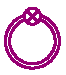
\includegraphics{qcd/diagrams/QCD-UFlow4.pdf}\end{gathered}
	+\frac{1}{2}\,\begin{gathered}
\includegraphics{qcd/diagrams/QCD-UFlow3.pdf}\end{gathered}
	-\,\begin{gathered}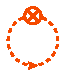
\includegraphics{qcd/diagrams/QCD-UFlow1.pdf}\end{gathered}
	-\,\begin{gathered}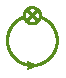
\includegraphics{qcd/diagrams/QCD-UFlow2.pdf}\end{gathered}\, ,
	\label{eq:QCDUflowDiag}\eqTagPrime
\end{align}
from fluctuating composites, gluons, ghosts, and quarks.
Using various projections and evaluating \cref{eq:QCDWetterich} on the \qeom{}, it is possible to derive flow equations for all \rgscaledependent{} couplings of the ansatz \eqref{eq:GammaQCD}, see 
\ccite{FuQCDRev,FuQCD} for details and the corresponding flow equations.
Solutions to the \qeom{}
\begin{subequations}\label{eq:QCDchiEval}
\begin{align}
	\FSsfEoM{}=\MFEchi{}&\equiv(\MFEphi,\MFEA,\MFEc,\MFEcb,\MFEpsi,\MFEpsib)\\
	&=((\sigma,0,0,0),(0,0,0,\MFEA_4),0,0,0,0)\,,
\end{align}
\end{subequations}
with $\MFEA_4$ and $\MFEphi_0\equiv\sigma$ as the only, homogeneous, non-vanishing expectation values are considered.
This allows a study of both the confinement-deconfinement and the chiral phase transition.
The flow is initialized at an \uv{} initial scale of $\Lambda = 20\,\GeV$ with the only input being the strong coupling constant $\alpha_{s,\Lambda}$ and parameters for the explicit chiral symmetry breaking due to quark masses, see Tab.~I of \ccite{FuQCD} for details.

\paragraph{Four-fermi couplings, dynamical hadronization, and \texorpdfstring{$\chi$SB}{cSB}}\phantomsection\label{paragraph:qcdDynHad}\mbox{}\\%
During the \rgscaleevolution{} from the \uv{} to the \ir{}, the four-fermi interactions of $\Lqbqqbq$ in \cref{eq:qcdLqbqqbq} get generated by quark-gluon interactions 
$\lambda_{\psi,k}\propto\alpha_{s,k}^2$ and get enhanced once generated by mixed terms $\lambda_{\psi,k}\propto\lambda_{\psi,k}\alpha_{s,k}$ and $\lambda_{\psi,k}\propto\lambda_{\psi,k}^2$:
\begin{align}
\partial_t \lambda_{\psi,k}=
\partial_t\begin{gathered}
\includegraphics{qcd/diagrams/QCD-4q.pdf}\end{gathered} &= \tilde{\partial}_t \Bigg(
\frac{1}{2}\,\begin{gathered}
\includegraphics{qcd/diagrams/QCD-4qFlow1.pdf}\end{gathered}+\ldots
+\frac{1}{2}\,\begin{gathered}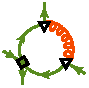
\includegraphics{qcd/diagrams/QCD-4qFlow5.pdf}\end{gathered}+\ldots
+\frac{1}{2}\,\begin{gathered}
\includegraphics{qcd/diagrams/QCD-4qFlow4.pdf}\end{gathered}+\ldots
\Bigg)\,,\label{eq:qcd4fermiFlow}
\end{align}
where we used the \rgtime{} derivative $\tilde{\partial}_t$ which acts only on regulators, \cf{} \cref{eq:dtTildeG} and the corresponding discussion.

In principle all four-fermi interaction channels with $SU(N_c=3)\otimes SU(2)_{\suR}\otimes SU(2)_{\suL}\otimes U(1)_{\suV}$ symmetry are generated, which for $N_f=2$ corresponds to a Fierz-complete set of ten four-fermi channels, see, \eg{}, \ccite{\qIVfierz} and Sec.~III.A and App.~B of \nbccite{FuQCDRev}. 
In this work we will focus solely on the $\sigma-\pi$ ($0^+(0^+)$ isoscalar, scalar $-$ $1^-(0^-)$ isovector, pseudoscalar) channel, which is crucial for the dynamics of \csb{}.
Studies including the Fierz-complete set of four-fermi couplings have shown, that the $\sigma-\pi$ channel dominates the dynamics, especially in the chiral limit for $N_f=2$ and 
$\mu_B/T\smallerlesssim 6$~\cite{Braun:2019aow,Fu:2019hdw,Fu:2022uow}.
It should be noted at this point, that especially at high chemical potentials and low temperatures ($\mu_B/T\smallergtrsim 6$) diquark and vector-meson channels gain importance
\cite{Braun:2017srn,Braun:2018bik,Braun:2019aow,Fu:2019hdw,Fu:2022uow}.
Diquark condensation and color superconductivity, see, \eg{}, \ccite{Buballa:2003qv,Alford:2007xm} for details, become very relevant for the phase structure of strongly interacting matter at high chemical potentials, \cf{} \cref{fig:qcdPDsketch}.
The interplay between inhomogeneous phases and color superconductivity might play an important role for \csb{}, see, \eg{}, \ccite{\inhomoCSC}.
That being said, we will focus solely on $\sigma-\pi$ channel in this work.

As the strong coupling increases towards lower \rg{}-/momentum-scales, \cf{} \cref{eq:alphagRunning}, four-fermi interactions become the dominant mode of interaction. 
Mainly diagrams $\lambda_{\psi,k}\propto\alpha_{s,k}^2$, \cf{} the first diagram in \cref{eq:qcd4fermiFlow}, lead to a shift of the dynamics from quark-gluon interactions towards quark-anti-quark scatterings.
This will be discussed further in the \customref{paragraph:qcdDec}{next paragraph}.

The $\sigma-\pi$ channel eventually becomes resonant at $k_{\chi}\approx 500\,\MeV$, signaling condensation and \csb{} in the $\sigma-\pi$ channel. 
When considering a momentum-independent four-fermi coupling $\lambda_{\psi,k}$, this condensation is signaled by a diverging $\lambda_{\psi,k}$ as $k\rightarrow k_{\chi}$.
The formation of a chiral condensate and \csb{} can be studied either by considering momentum-dependent four-fermi couplings, see, \eg{}, Sec.~III.A of \nbccite{FuQCDRev} for an overview, or by bosonizing the channel.\bigskip

In the latter approach the four-fermi channel gets bosonized by means of a \hsTrafoWithRefs{}, replacing the four-fermi interaction on a technical level by a Yukawa-type~\cite{Yukawa:1935xg} interaction of the form \eqref{eq:qcdLqbqphi}, \cf{} \cref{eq:gnHStrafo} \textit{ff.} for an explicit bosonization of the \gnm{}.
The complicated momentum-dependence of the resonant higher-order quark-anti-quark scatterings gets resolved elegantly in terms of meson exchanges. 

In the \frg{} such a bosonization can be implemented neatly and \rgscaledependent{}ly by means of \textit{dynamical hadronization}~\cite{Cyrol:2017ewj,Alkofer:2018guy,Fu:2019hdw}:
dynamical meson fields $\FSf{\Fphi}_k$ are introduced as quark-anti-quark composites in the generating functional \eqref{eq:ZkDef} with corresponding source terms $\FSf{J}^\phi \FSf{\Fphi}_k$.
As such they are pure auxiliary fields and their introduction does not spoil any \ir{} observables: when evaluating the \eaa{} in the \ir{} on the \qeom{}, \ie{}, $\FSf{J}^\phi=0$, one in fact recovers the original \ea{} of gauge fixed \qcd{}
\begin{align}
\Gamma_{\mathrm{QCD}}[\FSsf{}_f]=\Gamma_{k=0}[\MFphi_\eom[\FSsf{}_f],\FSsf{}_f]\,.
\label{eq:qcdAuxEom}
\end{align}
The composites are however extremely useful to study \csb{} and to elegantly extract related correlation functions.
The \rgscaledependent{} hadronization relation, \cf{} \cref{eq:dFSfdkConstraint}, employed for $\FSf{\Fphi}_k$:
\begin{align}
\langle\partial_t \FSf{\Fphi}_k \rangle_{k;\FSmf{J}}=\partial_t\MFphi_k \equiv \dot{A}_k\MFpsib \uIItv \MFpsi + \dot{B}_k\MFphi\,, \label{eq:qcdPhiHad}
\end{align}
can be considered as a successive bosonization of the quark-anti-quark channel, see Sec.~II.A of \nbccite{FuQCD} for further details including subtleties regarding explicit chiral symmetry breaking.
The so-called hadronization function $\dot{A}_k$ controls the overlap between the composites and the quark-anti quark channel.
The hadronization function $\dot{B}_k$ affects the wave-function renormalization $Z_\MFphi$.
Both $\dot{A}_k$ and $\dot{B}_k$ can be chosen freely to implement specific hadronization prescriptions. 
In \ccite{FuQCD} $\dot{B}_k=0$ is chosen and the renormalized and rescaled hadronization function $\dot{\bar{A}}_k\equiv \dot{A}_k k^2 Z_{\MFphi;k}^{1/2}/Z_{\MFpsi;k}$ is fixed by completely bosonizing the four-fermi interaction at all scales by enforcing 
\begin{align}
	\forall k\quad \bar{\lambda}_{\MFpsi;k}\equiv \frac{k^2}{Z_{\MFpsi;k}^2}{\lambda}_{\MFpsi;k} \hastobe0\,.
	\label{eq:qcd4fzero}
\end{align}
Diagrammatically this choice entails for the flow of the four-fermi coupling
\begin{align}
\partial_t\begin{gathered}
\includegraphics{qcd/diagrams/QCD-4q.pdf}\end{gathered} &= \tilde{\partial}_t \Bigg(
\frac{1}{2}\,\begin{gathered}
\includegraphics{qcd/diagrams/QCD-4qFlow1.pdf}\end{gathered}+\ldots
+\frac{1}{2}\,\begin{gathered}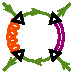
\includegraphics{qcd/diagrams/QCD-4qFlow2.pdf}\end{gathered}+\ldots
+\frac{1}{2}\,\begin{gathered}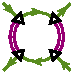
\includegraphics{qcd/diagrams/QCD-4qFlow3.pdf}\end{gathered}+\ldots
\Bigg)\,,\label{eq:qcd4fermiFlowHad}
\end{align}
where the diagrams $\propto\lambda_{\psi,k}^2$ and $\propto\lambda_{\psi,k}\alpha_{s,k}$ from \cref{eq:qcd4fermiFlowHad} vanish due to the hadronization constraint \eqref{eq:qcd4fzero}.
Further details and explicit flow equations can be found in Sec.~III.E  and the corresponding App.~L of \nbccite{FuQCD}.

This complete bosonization of the four-fermi coupling entails, that the complete dynamics of the $\sigma-\pi$ channel is encoded using the effective hadronic composites.
The emergent four-fermi coupling is on a computational level completely replaced by the Yukawa-type interaction of $\Lqbqphi$ from \cref{eq:qcdLqbqphi}, with multi scatterings of the resonant channel encoded in the effective potential $\LpotExpI$ of \cref{eq:qcdLpot}.
$\LpotExpI$ is directly related to the equilibrium thermodynamic grand potential density $\Omega$, see \cref{eq:thermalGrandPotentialDensity} of \cref{app:grandCanonicalPartitionFunction} and Sec.~III.F of \nbccite{FuQCD} for specifics. 
$\LpotExpI$ is the central quantity used to study \csb{} and the confinement-deconfinement transition.\bigskip

\fullWidthTwoColumnSubFigures%
	[!t] % Placement
	{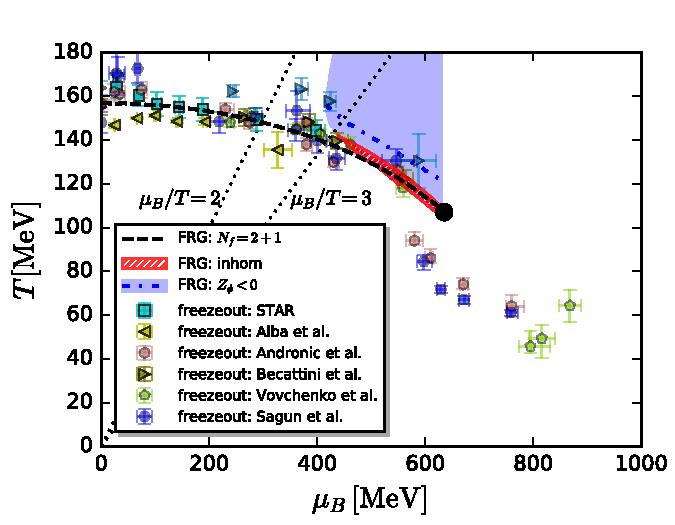
\includegraphics[width=\subcaptionFigureWidth]{qcd/figures/PhysRevD.101.054032Fig21noType3.pdf}} % left figure
	{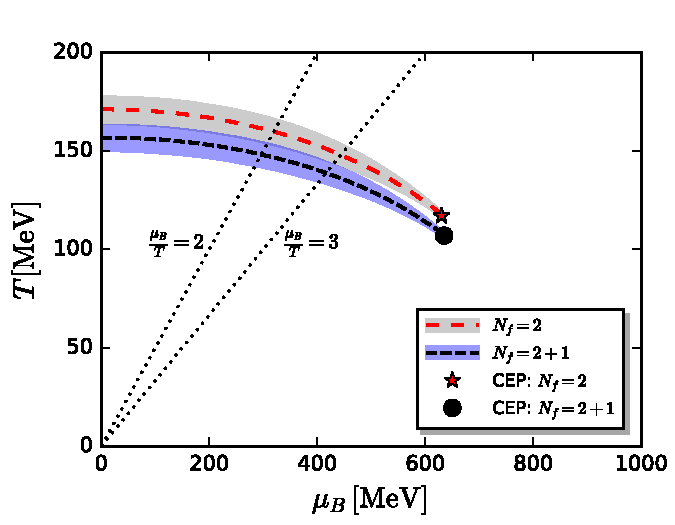
\includegraphics[width=\subcaptionFigureWidth]{qcd/figures/PhysRevD.101.054032Fig20noType3.pdf}} % Right figure
	[fig:fuQCDpd,fig:fuQCDpd2]
	{%
		Phase diagram of $N_f=2+1$ flavor \qcd{} including experimental freeze-out data~\cite{\qcdExpFreezeout} on the left \subref{fig:fuQCDpd} and $N_f=2$ and $2+1$ flavor \qcd{} phase diagram on the right \subref{fig:fuQCDpd2}.
		Information about the resulting and underlying (physical) parameters can be found in Tab.~I of \nbccite{Fu:2019hdw}.
		The red and blue regions on the left \subref{fig:fuQCDpd} are related to the possible emergence of inhomogeneous phases and are discussed in detail in \cref{subsec:inhomoLiterature}.
		The bands and dotted lines on the right \subref{fig:fuQCDpd2} mark the crossover region on temperature for the chiral condensate.
		An augmented version of the left figure \subref{fig:fuQCDpd} can be found in Fig. 13 of \ccite{Gao:2020qsj}, including lattice data~\cite{Boucaud:2018xup,Borsanyi:2020fev}, \dses{} results~\cite{Fischer:2014ata,Gao:2015kea}, and of course the results of \ccite{Gao:2020qsj} itself.
		\textit{Taken from the arXiv source for Fig. 21 and 20 of \ccite{Fu:2019hdw}.
		\ccbysaLicense{W.-j. Fu}}
	}%
	{fig:fuQCDpds}
At this point we want to comment and present one of the central results of \ccite{Fu:2019hdw}, the phase diagram of $N_f=2+1$ and $N_f=2$ flavor \qcd{} in \cref{fig:fuQCDpds} with realistic quark/pion masses and decay constants $f_\pi$ and $f_K$.
These phase diagrams must be considered seminal results and represent the culmination of a massive research effort by large parts of the \frg{} community towards such first principle results for \qcd{}.

The phase diagrams are computed up to $\mu_B/T\approx 6$ and include the chiral crossover transition between a \hbp{} at low temperatures and an approximately \symp{} at high temperatures.
The chiral crossover transition ends in a \cep{}.
Note that due to non-vanishing quark masses chiral symmetry only gets approximately restored and the transition is a smooth crossover instead of a second-order phase transition, which is found in the chiral limit.
The crossover temperatures at vanishing $\mu_B$ are found to be
\begin{align}
	T_{c,{\scriptscriptstyle{N_f=2}}}=171\,\MeV\,,\qquad T_{c,{\scriptscriptstyle{N_f=2+1}}} = 156\,\MeV\,,\label{eq:TC0qcd}
\end{align}
with a curvature $\kappa$ of the phase boundary $T_c(\mu_B)$ of
\begin{align}
	\kappa_{\scriptscriptstyle{N_f=2}}=0.0176(1)\,,\qquad \kappa_{\scriptscriptstyle{N_f=2+1}}=0.0142(2)\,,\label{eq:kappaQCD}
\end{align}
as the quadratic expansion coefficient of $T_c(\mu_B)$ around $\mu_B=0$:
\begin{align}
	\frac{T_c(\mu_B)}{T_c}&=1-\kappa \left(\frac{\mu_B}{T_c}\right)^2+\cdots\,.\label{eq:kappaTc}
\end{align}
The \ceps{} are located at
\begin{subequations}\label{eq:cepqcd}
\begin{alignat}{2}
	&(T_,\vts \mu_B)_{\scriptscriptstyle{\text{CEP},N_f=2}} &&= (117, 630)\,\MeV\,,\label{eq:cep2qcd}\\
	&(T_,\vts \mu_B)_{\scriptscriptstyle{\text{CEP},N_f=2+1}} &&= (107, 635)\,\MeV\,,\label{eq:cep3qcd}
\end{alignat}
\end{subequations}
which entails
\begin{subequations}\label{eq:zcepqcd}
\begin{alignat}{2}
	&(T/{\mu_B})_{\scriptscriptstyle{\text{CEP},N_f=2}} &&= 5.38\,,\label{eq:zcep2qcd}\\
	&(T/{\mu_B})_{\scriptscriptstyle{\text{CEP},N_f=2+1}} &&= 5.93\,.\label{eq:zcep3qcd}
\end{alignat}
\end{subequations}
A discussion of these results (and the values themselves) can be found in Sec.~V.D \dash{} Eqs.~(121)\dash{}(127) \dash{} of \ccite{Fu:2019hdw}.
Since we are primarily working with quark chemical potential $\mu$: note that $\mu_B=3\mu$ and thus $\kappa\rightarrow 9\kappa\equiv \kappa'$, \ie{}, $\kappa'_{\scriptscriptstyle{N_f=2}}=0.1584(9)$ in terms of $\mu$ instead of $\mu_B$ in \cref{eq:kappaQCD}.

The indication for inhomogeneous phases in \cref{fig:fuQCDpd} will be discussed in \cref{subsec:inhomoLiterature}.
The limitation of the results in \ccite{Fu:2019hdw} to $\mu_B/T\smallerlesssim 6$ has several reasons. 
One is the inclusion of only the scalar-pseudoscalar $\sigma-\pi$ channel \dash{} a discussion with qualitative and quantitative predictive power at $\mu_B/T \smallergtrsim 6$ should include at least the dominant diquark and vector-meson channels.
Another technical limitation of \ccite{Fu:2019hdw} is the application of a \frg{} Taylor expansion, \cf{} \teRef{}, for the effective potential $\LpotExpI$. 
A study of non-smooth, potentially first-order, chiral phase transitions requires \dash{} as we will argue throughout this work \dash{} proper shock capturing schemes for the underlying \pdes{}, \cf{} \ccite{Grossi:2019urj,zerod1,zerod2,zerod3,Ihssen2020,Grossi:2021ksl,Stoll:2021ori,Ihssen:2022xkr,Ihssen:2023xlp} and \cref{subsec:RGflow} as well as \cref{chap:zeroONSU2,chap:GN}.
In the context of \ccite{Fu:2019hdw} especially the recent work~\cite{Ihssen:2023xlp} represents significant progress in terms of an application of the recently developed \cfd{} perspective for \frg{} flow equations.

\FloatBarrier
\paragraph{Sequential decoupling and the emergence of NJL-/QMM-type LEFTs from QCD}\phantomsection\label{paragraph:qcdDec}\mbox{}\\%
\fullWidthTwoColumnSubFigures%
	[!t] % Placement
	{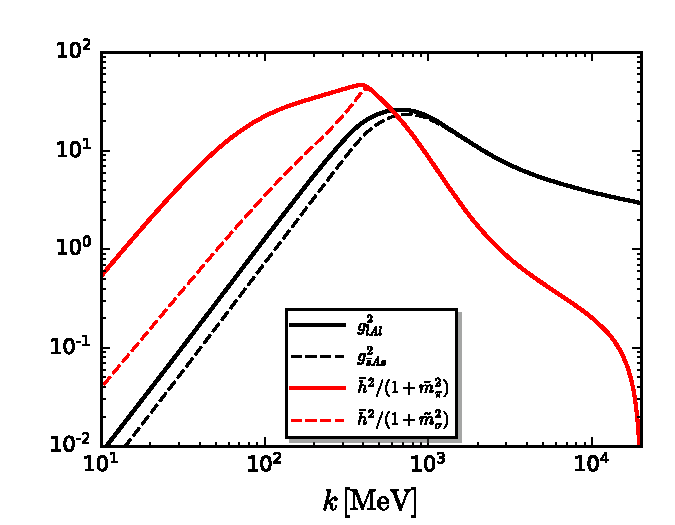
\includegraphics[width=\subcaptionFigureWidth]{qcd/figures/PhysRevD.101.054032Fig18noType3.pdf}} % left figure
	{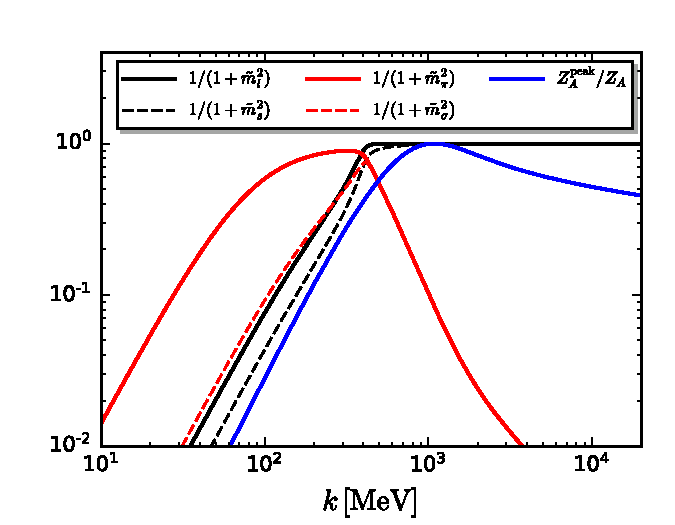
\includegraphics[width=\subcaptionFigureWidth]{qcd/figures/PhysRevD.101.054032Fig19noType3.pdf}} % Right figure
	[fig:fuQCDgh,fig:fuQCDgaps]
	{%
		Dimensionless four-quark single gluon couplings (in black) and dimensionless four-quark single meson exchange couplings (red) on the left \subref{fig:fuQCDgh} and
		dimensionless propagator gaps for quarks (in black), mesons (in red), and a gluon dressing function for comparison (in blue) on the right \subref{fig:fuQCDgaps}.
		\textit{Taken from the arXiv source for Fig. 18 and 19 of \ccite{Fu:2019hdw}.}
		\ccbysaLicense{W.-j. Fu}
	}%
	{fig:fuQCDdecoupling}
One extremely interesting and for our work relevant observation in \ccite{Fu:2019hdw} is the observed \textit{sequential decoupling of dynamic, relevant degrees of freedom} during \rgscale-evolution from the \uv{} towards the \ir{}.
The phenomenon is visualized in \cref{fig:fuQCDdecoupling} and described at length in Sec.~V.D of \ccite{Fu:2019hdw}.
We will give a concise summary here using \cref{fig:fuQCDdecoupling}.

\Cref{fig:fuQCDgh} includes dimensionless quark-gluon couplings and dimensionless quark-meson couplings and we can observe, that the quark-gluon coupling dominates in the \uv{} for scales 
$k\smallergtrsim 1\,\GeV$.
In turn, for scales $k\smallerlesssim 1\,\GeV$, the quark-meson couplings gain importance and become dominant at $k\approx 0.6\,\GeV$, while the quark-gluon couplings decay rapidly \dash{} note the logarithmic scale on the vertical axis of \cref{fig:fuQCDgh}.
This observation is further supported by considering the propagator gappings in \cref{fig:fuQCDgaps}: the gluons decouple first only followed by the quarks and mesons.
First the gluonic dynamics decouples from the matter sector, followed by the quark- and \sigmaModes{} and ultimately the pion decouples last.
Note the dominance of pions for the dynamics at low \rgscales{} $k\approx 0.2\,\GeV$.
The connection and emergence of chiral perturbation theory in vacuum in this context is discussed in \ccite{Eser:2018jqo,Divotgey:2019xea,Eser:2019pvd}.
We will discuss the dynamics of such pionic modes in comparison to radial \sigmaModes{} at length in our study of zero-dimensional $O(N)$ models in \cref{subsec:0dONresults}.
The discussion of the interplay of bosonic and fermionic fluctuations is at the heart of our study of the \gn{} model at finite $N$ in \cref{subsec:gnyFiniteNresults} and we observe a similar decoupling hierarchy between fermionic and bosonic modes in this low-dimensional model.

This sequential decoupling of dynamic/relevant degrees of freedom gives rise to an intriguing and for the \frg{} practitioners extremely attractive point of view: first principle \frg{} \qcd{} computations~\cite{Fu:2019hdw} show, that the highly complicated and involved gauge-dynamics of \qcd{} decouples for low \rgscales{} $k\approx 1\,\GeV$. 
Furthermore, by employing dynamic hadronization, we observe the emergence of Polyakov loop enhanced \loefts{}, see, \eg{}, \ccite{Braun:2015fva,Schaefer:2007pw,Haas:2013qwp}.
With the currently discussed hadronization prescription, \viz{} the \pqmm{} emerges.
The relevant dynamic degrees of freedom, \viz{} quarks and mesons (as quark-anti-quark composites), and their interactions at $k\smallerlesssim1\,\GeV$ are properly captured by \loefts{} like the \pqmm{}.
Studies like \ccite{Fu:2019hdw} allow for \textit{QCD-assisted} \loefts{}: using full fledged, first principle \frg{} computations for \qcd{} to initialize \loefts{} like the \pqmm{} at scales $k\smallerlesssim 1\,\GeV$.
Typically such theories have been used as low-energy effective models by fitting vacuum observables to determine model parameters, \cf{} \cref{sec:cdwmf} and, \eg{}, \ccite{Schaefer:2007pw}.
The maturing \frg{} computations for \qcd{} can be used to eliminate the need for such parameter fits by providing input for the model parameters from first principle \qcd{} flows.
Thus promoting them from \textit{``mere effective models''} to \textit{QCD-assisted} \loefts{}.
First steps of such improvements can be found in \ccite{Haas:2013qwp,Herbst:2013ufa,Springer2017} and the more recent works~\cite{Leonhardt:2019fua,Ihssen:2023xlp}.

\subsubsection{The quark-meson model}\label{subsubsec:qcdQMM}
We want to conclude our introduction into \qcd{} and \loefts{} by actually introducing the \loeft{} we will be using in \cref{chap:QMM}: the \acrrepeatEmph{qm} model, sometimes also referred to as linear-$\sigma$ model. 
The \qmm{} and variants/extensions of it \dash{} including the \pqmm{} \dash{} are incredibly popular in the field of theoretical \hep{}.
An extensive review of the vast literature regarding the model is beyond the scope of the current work.
At this point we only want to reference the very incomplete list of \qmm{} \frg{} literature~\cite{Ellwanger:1994wy,Schaefer:2004en,Rennecke:2016tkm,Fu:2018qsk,Alkofer:2018guy,Tripolt:2017zgc,Eser:2018jqo,Divotgey:2019xea,Eser:2019pvd,Grossi:2021ksl,Ihssen:2023xlp}.
For a review of primarily mean-field/large-$N_c$ results we refer to \ccite{Scadron:2013vba} and for a review of \frg{} studies with the \qmm{} we refer to Sec.~III.B of \nbccite{Fu:2022gou}.
Additional/complementary references to the ones provided in \ccite{Fu:2022gou} may be found in the last line of the fourth-to-last paragraph of Sec.~V.C of \nbccite{Fu:2019hdw}.\bigskip

In this work we consider the $N_f=2$ flavor \qmm{}, which in the present context, emerges as the part of \cref{eq:GammaQCD} relevant for the dynamics at low \rgscales{} $k\smallerlesssim 1\,\GeV$.
The \qmm{} is formed by $\mathcal{L}_{\MFpsib\MFpsi}[\mkern1.5mu{}\xcancel{\MFA}\mkern1.5mu{},\MFpsi,\MFpsib\mkern0.5mu{}]$, $\Lqbqphi$, $\LphiKin$, and $\mathcal{L}_{V}[\mkern1.5mu{}\xcancel{A}\mkern1.5mu{},\MFphi]$ from \cref{eq:qcdLqbqKi,eq:qcdLqbqphi,eq:qcdLphiKin,eq:qcdLpot}.
We will consider it primarily in \lpa{}, \cf{} \deRef{}, and without considering the statistical confinement provided by the Polyakov loop potential.
To get specific, we study the following \eaa{},
\begin{align}
\FSeaa_k^\mathrm{QMM}[\FSmf{\FSsf}]\equiv \intx[x]\,\bigg( 
\MFpsib(\gamma_\mu \partial_\mu -\gamma_4\mu + h \MFphi_i \uIItv^{i} )\MFpsi
+\frac{1}{2}\big(\partial_\mu\MFphi\big)^2
+U_{k}(\MFrho)
\bigg)\,,
\label{eq:QMMeaa}
\end{align}
with the field-independent, constant Yukawa coupling $h$ and the scale-dependent mesonic self-interaction potential $U_k(\MFrho)$ as a function of the $O(4)$ invariant $\MFrho\equiv\frac{1}{2}\MFphi^2$. 
In $\FSmf{\FSsf}\equiv(\MFphi,\MFpsi,\MFpsib)$ we consider four dynamic, on this level fundamental, mesons $\MFphi=\langle\Fphi\rangle\equiv (\MFphi_0,\pi_1,\pi_2,\pi_3)$ and $N_c=3$ dynamic quarks $\MFpsi=\langle\Fpsi\vts\rangle$ and $\MFpsib=\langle\Fpsib\vts\rangle$ with $N_f=2$ flavors.

The \qmm{} \dash{} its \eaa{} \eqref{eq:QMMeaa} in \lpa{} \dash{} shares the chiral symmetry
\begin{align}
SU(2)_{\suL}\otimes SU(2)_{\suR}\otimes U(1)_{\suV} \simeq SU(2)_{\suV}\otimes SU(2)_{\suA}\otimes U(1)_{\suV}
\label{eq:QMMchiral}
\end{align}
with \qcd{}, see \cref{paragraph:qcdChiral}.
The model, especially in the context of a \textit{QCD-assisted} \loeft{}, is ideally suited to study the dynamics of \csb{}.
For the mesons chiral symmetry manifests through the equivalence $SU(2)_{\suL}\otimes SU(2)_{\suR} \simeq SO(4)$ as an $SO(4)$ symmetry, which motivates the $O(4)$ vector
\begin{align}
\MFphi \equiv (\varphi_0,\pi_1,\pi_2,\pi_3)\,,
\label{eq:phiVector}
\end{align}
with the $1^-(0^-)$ isovector, pseudoscalar pions\footnote{%
	Note that we are referring here to flavor eigenstates with $(\pi_1,\pi_2,\pi_3)$.
	The charge eigenstates $\pi_\pm$ and $\pi_0$ can be obtained in the usual manner $\pi_\pm=(\pi_1\mp \iu \pi_2)/\sqrt{2}$ and $\pi_{0}=\pi_3$.
} and the $0^+(0^+)$ isoscalar, scalar $\MFphi_0$/$\sigma$\footnote{
	We reserve the symbol $\sigma$ in equations and expressions for the value we evaluate $\MFphi_0$ on, \ie{}, the possible solution of $\MFphi_{0;\eom}\equiv\sigma$ we probe for.
	This distinction will become clearer with the applications in the main part of this thesis in \cref{chap:zeroONSU2,chap:GN,chap:QMM}.
	In the text we will usually refer to the zeroth component of $\MFphi$ as radial, massive, or \sigmaMode{} depending on the context.
}.
The pions are in the isospin triplet $SU(2)_\suV\simeq SO(3)$ and are the Nambu-Goldstone bosons of the $SU(2)_\suA$ chiral symmetry breaking, which manifests in the mesonic sector as a breakdown of $SO(4)$ to $SO(3)$ with the radial $\MFphi_0$ as massive \sigmaMode{}.

We will reserve further discussions for the applications in \cref{chap:QMM} apart from one last remark at this point regarding $U(1)_\suA$ symmetry in the $N_f=2$ \qmm{}.
For $N_f=2+1$ flavors the anomalous $U(1)_\suA$ symmetry breaking, mentioned in \cref{paragraph:qcdChiral}, is usually included in the three flavor \qmm{} by means of a t'Hooft determinant~\cite{tHooft:1976rip}, see, \eg{}, \ccite{Schaefer:2008hk,Scadron:2013vba,Rennecke:2015lur,Rennecke:2016tkm,Braun:2018bik}.
It is a determinant in flavor space resulting in a six-point interaction and it is crucial to properly reproduce the aforementioned $\eta-\eta'$ mixing~\cite{Kobayashi:1970ji,Kobayashi:1971qz,DelDebbio:2004ns,Luscher:2010ik,Ce:2014sfa}.
In the $N_f=2$ case such a determinant manifests, in terms of quark-anti-quark bilinears, as an ordinary four-fermi coupling
\begin{align}
 \mathcal{O}^{(S+P)_{-}}_{ijlm}{\MFpsib}_i\MFpsi_j{\MFpsib}_l\MFpsi_m=&(\MFpsib\,t^0 \MFpsi)^2+(\MFpsib\,\gammach t^0 \MFpsi)^2 -(\MFpsib\,t^a \MFpsi)^2-(\MFpsib\,\gammach t^a \MFpsi)^2\,,\label{eq:QMMSpPm}
\end{align}
where we adapted the notation of App.~B of \nbccite{Fu:2022gou}.
The $N_f=2$ \qmm{} is constructed (in terms of Fierz-complete couplings) by the linear combination (sum) of \cref{eq:QMMSpPm} with the $U(1)_\suA$-symmetric channel
\begin{align}
 \mathcal{O}^{(S-P)_{+}}_{ijlm}{\MFpsib}_i\MFpsi_j{\MFpsib}_l\MFpsi_m=&(\MFpsib\,t^0 \MFpsi)^2-(\MFpsib\,\gammach t^0 \MFpsi)^2+(\MFpsib\,t^a \MFpsi)^2-(\MFpsib\,\gammach t^a \MFpsi)^2\,\label{eq:QMMSmPp}\, .
\end{align}
Such a linear combination completely eliminates/decouples the three $1^-(0^+)$ isovector, scalars $\MFpsib\,t^a \MFpsi$ and the $0^+(0^-)$ isoscalar, pseudoscalar $\MFpsib\,\gammach t^0 \MFpsi$ as the chiral partners of the pions and $\sigma$.
In that sense $U(1)_\suA$ is ``maximally broken'' in the $N_f=2$ flavor \qmm{}~\cite{Rennecke:2015lur}.
Phenomenologically these chiral partners correspond to the heavy $a_0$ and $\eta_N$ mesons \dash{} with $m_{a_0}\approx 980\,\MeV$~\cite{ParticleDataGroup2022Aug} and $\eta_N$ not really observable (only as a mixture/part of $\eta$/$\eta'$).
For the dynamics of $N_f=2$ \csb{} those heavy partners are not relevant and are thus usually not considered in the $N_f=2$ \qmm{}.
\section{Inhomogeneous (chiral) condensates}\label{sec:inhomogeneousPhases}
With this section we will conclude the methodological introductions of this chapter, by providing a concise introduction to inhomogeneous chiral condensates  $\chiCond(\vec{x}\vts)$.
We will mainly focus on computational challenges, employed methods, and selected literature results of particular relevance for this work, \ie{}, for \cref{chap:GN,chap:QMM}.
This section is compiled from various Refs.~\cite{Carignano:2012yli,Buballa:2014tba,Motta:2023pks,Stoll:2021ori,Koenigstein:2021llr,A03first:2016,A03second:2021}, which informed our discussion here and have served as sources for most of the referenced publications.\bigskip

A lot of studies in the field of theoretical \hep{} of the phase structure of strongly interacting systems are based on the tacit assumption that the involved condensates 
-- \ie{}, mean-fields, expectation values, solutions for the \qeom{}/gap equation \dash{} do not vary in space $\vec{x}$ and (Euclidean) time $(\tau)$ $t$.

Before continuing with our discussion of inhomogeneous condensates, \viz{} condensates that vary only in space $\vec{x}$ and not in (Euclidean) time  $(\tau)$ $t$, we want to comment on the explicit assumption of (Euclidean) time-independent condensates.
The possibility of time-dependent condensates in the context of \hep{} has been brought forward by Frank Wilczek and Alfred Shapere with their proposition of quantum and classical \textit{time crystals}~\cite{Wilczek:2012jt,Shapere:2012nq} in 2012. 
The proposition of such time-dependent ground states for time-independent systems has sparked intensive research and scientific discourse, see, \eg{}, the review~\cite{Sacha:2017fqe} for an overview.
Both real and imaginary time crystals have been considered and their relation and connection at non-zero temperature has been explored.
Through the years a consensus has been reached, especially with important contributions in \ccite{Bruno:2013mva,Watanabe:2014hea}, that such time crystals do not appear as energetically favored ground states of time-independent systems, \ie{}, there is no spontaneous breaking of (Euclidean) time-translation invariance~\cite{Sacha:2017fqe}.
There is however still quite intensive research, see, \eg{}, \ccite{Nissinen2017Aug,Kinoshita:2017uch,Gorsky:2019fdi,Arouca:2021jar}, into such states in exited and especially externally driven systems. 
For our work however those scenarios are not relevant and we will limit our discussion to only spatially varying inhomogeneous condensates.

The general phenomenon of inhomogeneous phases/condensates in dense and strongly interacting systems is certainly not a new one.
Especially in the field of solid-state physics inhomogeneous condensates \dash{} charge density waves \dash{} in superconductors related to the Peierls instability~\cite{Peierls1996Aug} are well know, with pioneering works by Peter Fulde and Richard A. Ferrell~\cite{Fulde:1964zz} (1964) as well as by Anatoly Larkin and Yuri Ovchinnikov~\cite{Larkin:1964wok} (1965), see, \eg{}, the reviews~\cite{Gruner:1994zz,Monceau_2012,Pouget2016Mar} for further details on charge density waves.
The idea of density waves in nuclear matter and pion condensation was already discussed in the 1960s and 1970s by Albert Overhauser, Arkadi B. Migdal, Francois Dautry, Ebbe M. Nyman, and others~\cite{Overhauser1960Apr,Migdal1973Jul,Migdal1978Jan,Dautry:1979bk}.

In the 1990s these concepts were first applied to quark matter by Wojciech Broniowski, Andrzej Kotlorz, Marek Kutschera, and others~\cite{Broniowski:1990dy,Deryagin:1992rw,Shuster:1999tn,Sadzikowski:2000ap} in their studies of chiral quark models.
In the early 2000s there has been a lot of research of \cosc{} phases, see, \eg{}, the reviews~\cite{\cscReview}, also including studies~\cite{\cscRefs} of crystalline \cosc{} phases.
These findings triggered a renewed interest, see, \eg{}, \ccite{Nakano:2004cd,Nickel:2009ke,Nickel:2009wj,Abuki:2011pf}, in inhomogeneous chiral condensates~\cite{Buballa:2014tba}.
Also the interplay between \cosc{} and chiral phases has been explored, see, \eg{}, \ccite{\inhomoCSC}.

Parallel studies~\cite{\inhomoTwoD} in \twoDimensional{} chiral models, especially in the \gnm{}~\cite{Gross:1974jv}, have firmly established inhomogeneous chiral condensates in such low-dimensional models in the mean-field/infinite-$N$ limit.
Inhomogeneous phases have also been shown to appear in imbalanced Fermi gases~\cite{\inhomoFermiGases}.\bigskip

The aforementioned research efforts lead to the realization, see, \eg{}, the review~\cite{Buballa:2014tba}, that inhomogeneous chiral condensates $\chiCond(\vec{x}\vts)$ are an important and rather robust feature in chiral models like the \acrrepeat{njl} model and \acrrepeat{qm} model.
The predominantly mean-field and large-$N_c$ computations and their findings in these models are in parts supported by some (in this context exploratory) \frg{}, \dses{}, and weak-coupling studies of \qcd{} and its \loefts{}~\cite{Deryagin:1992rw,Shuster:1999tn,Muller:2013tya,Tripolt:2017zgc,Fu:2019hdw}.
The phase structure of \qcd{} \dash{} including the question of inhomogeneous chiral condensation \dash{} is still not fully understood at intermediate temperatures and densities, see \cref{chap:introduction} and the previous \cref{sec:qcdModels}.
We will present and discus some of the relevant literature results for inhomogeneous chiral condensates in \cref{subsec:inhomoLiterature}.

In general it can however be noted, that it is an open question whether inhomogeneous chiral condensates exist beyond mean-field. 
It remains unclear whether, bosonic thermal and quantum fluctuations \dash{} which are neglected in mean-field and large-$N_c$ computations \dash{} could destabilize inhomogeneous chiral condensates.
These condensates are formed, in the first place, by thermodynamic fermionic fluctuations, \cf{} \cref{chap:GN,chap:QMM}.

Another question that arose with \ccite{Buballa:2020nsi,Pannullo:2022eqh,Pannullo:2023one,Pannullo:2023nonint} and related earlier works~\cite{Broniowski:1990gb,Partyka:2008sv}, is whether and to 
what extent the appearance of inhomogeneous chiral condensates depends on regularization.
In certain studies with a finite cutoff, the emergence of inhomogeneous chiral condensates has to be regarded as a cutoff artifact, rather than a physical phenomenon~\cite{Buballa:2020nsi,Pannullo:2022eqh,Pannullo:2023one,Pannullo:2023nonint}.
This is why we choose to investigate inhomogeneous phases in renormalizable models \dash{} \gnm{} and \qmm{} \dash{} in \dtwo{} and \dfour{} in \cref{chap:GN,chap:QMM}.
Especially in our \mf{} studies of the \qmm{} we elaborate on the role of cutoffs/\uv{} initial scales and the importance of \rgcy{} in this context, \cf{} \cref{subsec:RGconsistency,sec:cdwmf}.
Ultimately, the goal is to move away from model studies and instead focus on \textit{QCD-assisted} \loefts{}~\cite{Fu:2019hdw, Leonhardt:2019mpy, Ihssen:2023xlp}, as discussed in \cref{subsec:chiralLEFT}.

\subsection{Technical challenges and methods}\label{subsec:inhomoMethods}
The main technical challenge arising when studying inhomogeneous chiral condensates $\chiCond(\vec{x}\vts)$, is the fact that the involved two-point functions manifest with explicit position-dependencies. In momentum space this translates to a non-diagonal, complicated coupling of different spatial momenta.
One such explicit situation is discussed in \cref{chap:QMM} for the \cdw{} condensate \eqref{eq:cdw} and the corresponding fermionic and bosonic two-point functions in \cref{eq:cdwGF,eq:cdwGB}.
Computations within \qft{} (especially functional and related approaches) usually involve the inversion of such two-point functions to compute propagators.
This is simply not possible with standard techniques when inhomogeneous phases are involved due to the complicated coupling of different spatial momenta.\bigskip

In the following we will list some of the methods that have been adapted or developed to study inhomogeneous phases. We distinguish between direct methods, which involve explicit computations with inhomogeneous condensates and indirect methods, which do not include such explicit computations.
Examples of direct methods are:
\begin{itemize}
	\item \textbf{Specialized analytic and semi-analytic methods} exist for certain models, truncations (usually large-$N$), and condensate shapes, allowing for direct computations. 
	In the field of \hep{} the most prominent examples of such methods are the studies~\cite{\inhomoTwoD} in \dimPlus{1}{1} dimensions and computations using the \cdw{}, like, \eg{}, \ccite{\cdwHEP}.
		\item \textbf{Lattice simulations} use a discretization of space-time in position space to tackle the problem by discretization, see, \eg{}, \ccite{Pannullo:2019bfn,Pannullo:2019prx,Lenz:2020bxk,Lenz:2020cuv,Lenz:2021vdz,Lenz:2021kzo} for recent results of this developing field.
	\item \textbf{Lattice field theory} uses the same discretization in position space but does not consider fluctuations beyond a saddle-point expansion, see, \eg{}, \ccite{deForcrand:2006zz,Pannullo:2021edr,Winstel:2021yok,Winstel:2022jkk} for applications and details.
	\item \textbf{Mode expansions} are basically the momentum-space analog to lattice field theory, see, \eg{}, \ccite{Wagner:2007he,Heinz:2015lua,Carignano:2012yli} for applications and details.
\end{itemize}

\clearpage
Examples for indirect methods are:
\begin{itemize}
	\item \textbf{A stability analysis} of the homogeneous ground state against inhomogeneous fluctuations is by far the most common indirect way to study inhomogeneous phases, see, \eg{}, \ccite{\stabRefs}.
	\item \textbf{Generalized Ginzburg-Landau/Gradient expansions} are closely related to the former but usually employ a simpler expansion approach, see, \eg{}, \ccite{\gglRefs}.
\end{itemize}
We will comment and elaborate on these methods further especially in \cref{chap:GN,chap:QMM}.
For a comprehensive overview we again refer to literature: \ccite{\inhomoReviews} and the reviews~\cite{Broniowski:2011ef,Buballa:2014tba}.

\FloatBarrier
\subsection{Literature results}\label{subsec:inhomoLiterature}
In this subsection we want to present a very limited subset of the aforementioned results in form of relevant figures for this thesis.\bigskip

First we present the original version~\cite{Thies:2003kk} of the inhomogeneous phase diagram of the \gnm{} in \cref{fig:GNthisPD}. This result will be discussed at length in \cref{sec:gnInfInhomo} and has to be considered one of the most influential direct results.

We continue with a series of phase diagrams for the \qmm{} with \cdw{} condensates at infinite $N_c$.
\Cref{fig:QMBroniowskiPD} is the pioneering study~\cite{Broniowski:1990dy} of Broniowski \etal{} and \cref{fig:QMMsMFAref,fig:QMMrMFAref} from~\cite{Adhikari:2017ydi} are basically the current reference values for the standard mean-field diagram (disregarding vacuum fermionic vacuum fluctuation) and the completely renormalized \qmm{} phase diagram including fermionic fluctuations completely.
\Cref{fig:QMMsMFAref,fig:QMMrMFAref} can at this point be considered conclusive results in the respective scenarios.

The last two sets of figures are the \frg{} results mentioned earlier which influenced the discussion in this thesis immensely.
The negative values for the bosonic wave-function renormalization of \cref{fig:qcdZphis}, found in the phase diagram of \qcd{} \cref{fig:fuQCDpds}, signal the possibility for an instability of the homogeneous ground state against inhomogeneous condensation. The role of $Z<0$ as an indicator for inhomogeneous phases is discussed in detail in \cref{paragraph:GNZphi}.

\Cref{fig:QMMarno} displays related results from a \frg{} based stability analysis of the \qmm{} in \lpa{}, with \cref{fig:QMMarno1} showing clear indications for an instability towards inhomogeneous condensation during the \frg{} flow.
\Cref{fig:QMMarno2} marks a large region in the phase diagram where the pion two-point function develops such instability towards inhomogeneous condensation during the \frg{} flow.
Whether or to what extent the instability at non-zero $k$ persists or manifests in the \ir{} limit ${(k\rightarrow 0)}$ is not fully settled yet.

\fullWidthTwoColumnSubFigures%
	[!t] % Placement
	{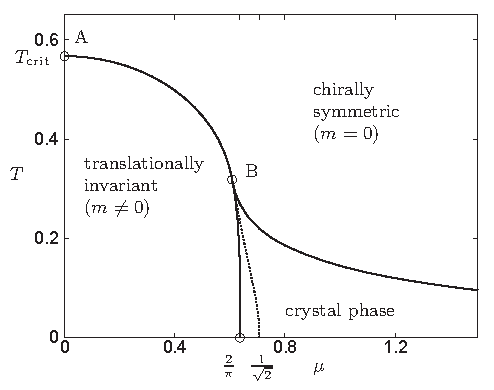
\includegraphics[width=\subcaptionFigureWidth+0.5cm]{inhomo/figures/PhysRevD.67.125015Fig8.pdf}} % left figure
	{\hspace{.3cm}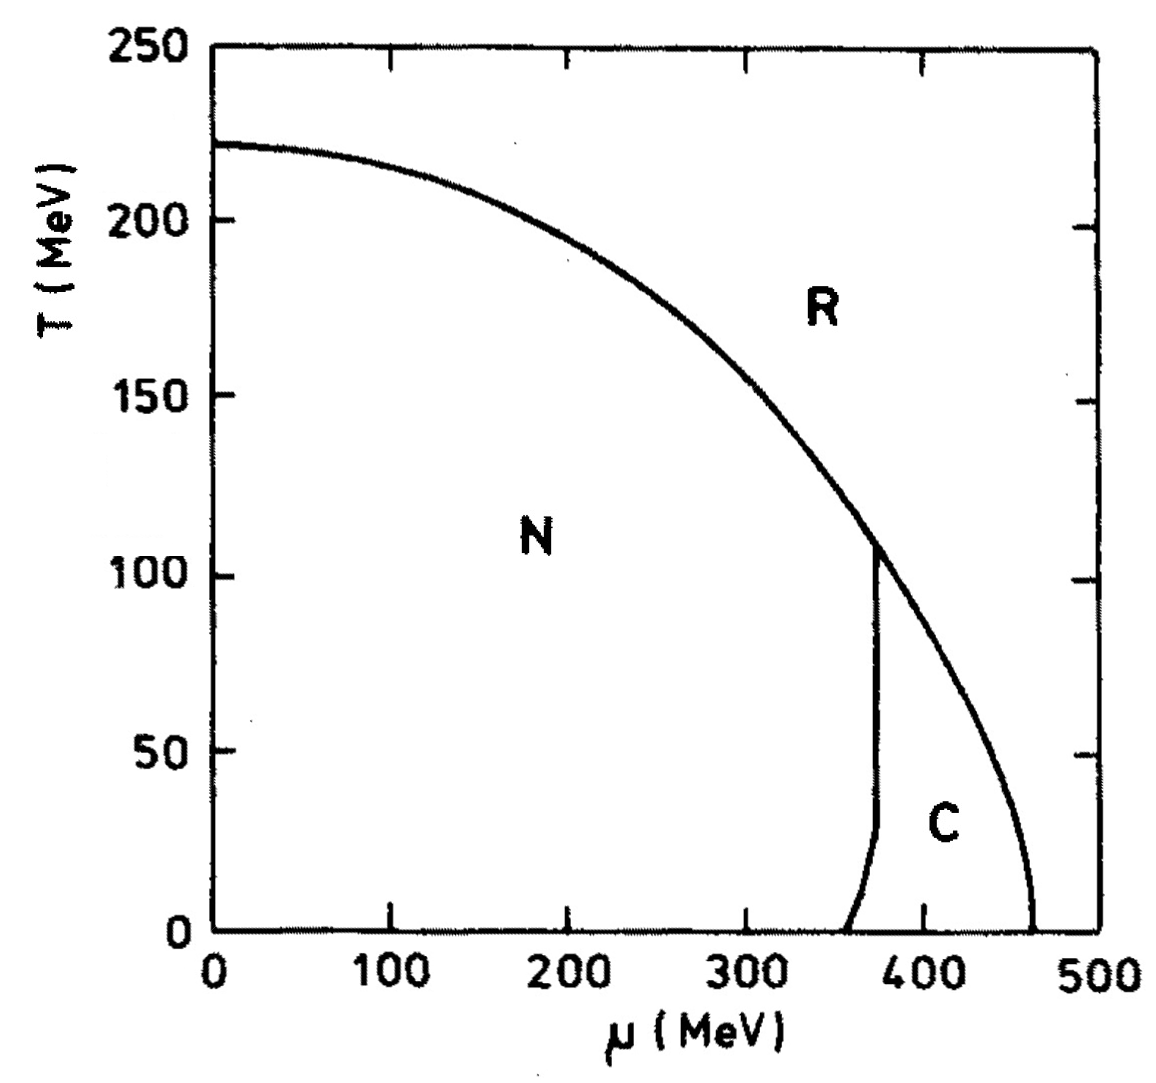
\includegraphics[width=\subcaptionFigureWidth-0.55cm]{inhomo/figures/Acta Phys.Polon.B.22.145Fig8u.png}} % Right figure
	[fig:GNthisPD,fig:QMBroniowskiPD]
	{%
		Exact/semi-analytic result~\cite{Thies:2003kk} for the inhomogeneous phase diagram of the \gnm{} at infinite $N$ in \dimPlus{1}{1} dimensions on the left \subref{fig:GNthisPD}.
		Pioneering mean-field study~\cite{Broniowski:1990dy} of the \qmm{} allowing for \cdw{}-type condensates, considering only fermionic vacuum fluctuations at large $N_c$ on the right \subref{fig:QMBroniowskiPD}.
		The difference between this and the revised version in \cref{fig:QMMsMFAref}, is that in the original work no in amplitude and wave vector-independent minimization was performed.
		Hence the correct inhomogeneous ground state is not found. Nevertheless, the impact of \ccite{Broniowski:1990dy} in the study of inhomogeneous phases with the \cdw{} is immense.
		\textit{Taken from the arXiv source for Fig. 8 of \ccite{Thies:2003kk} and from the upper panel of Fig 8 of \ccite{Broniowski:1990dy} but for the presentation here we flipped the axes in the latter using Photoshop CS6~\cite{photoshopCS6}.}
		\ccbysaLicense{M. Thies and W. Broniowski}
	}%
	{fig:inhomoPDs}
\fullWidthTwoColumnSubFigures%
	[!t] % Placement
	{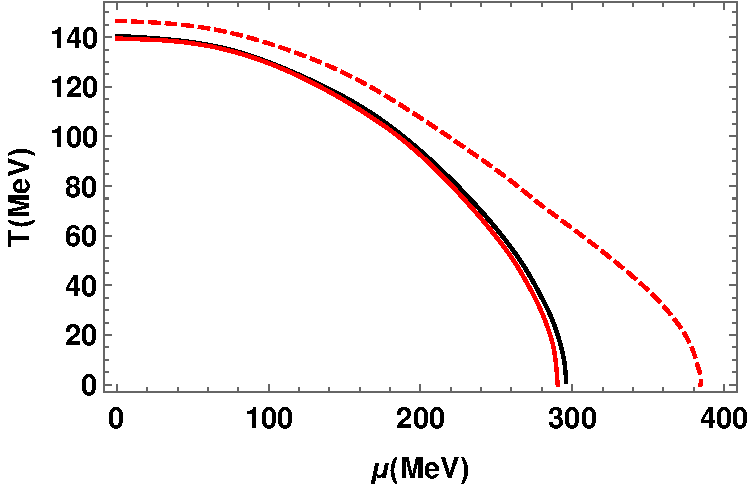
\includegraphics[width=\subcaptionFigureWidth]{inhomo/figures/PhysRevD.96.016013Fig2.pdf}} % left figure
	{\hspace{.3cm}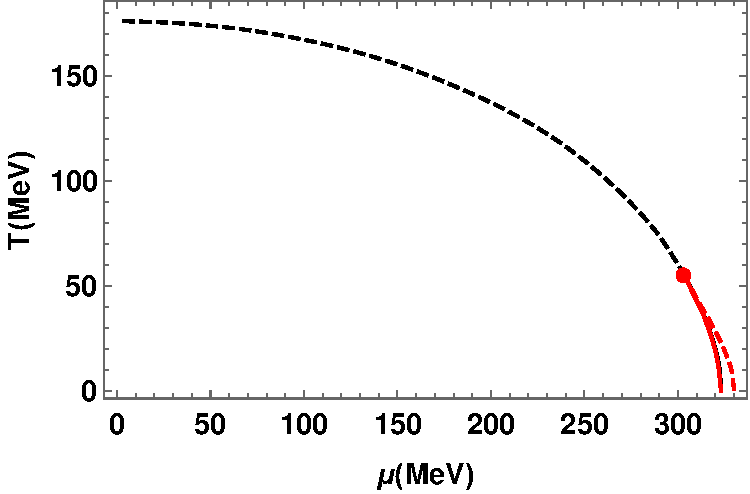
\includegraphics[width=\subcaptionFigureWidth]{inhomo/figures/PhysRevD.96.016013Fig3.pdf}} % Right figure
	[fig:QMMsMFAref,fig:QMMrMFAref]
	{%
		Improved version~\cite{Adhikari:2017ydi} of \cref{fig:QMBroniowskiPD} on the left \subref{fig:QMMsMFAref}: standard mean-field results for the \qmm{} disregarding vacuum fluctuations.
		Renormalized mean-field result for the \qmm{} on the right \subref{fig:QMMrMFAref} including all fermionic fluctuations completely.
		The black lines are the homogeneous reference results, the red lines are the inhomogeneous computations, and the solid (dashed) lines mark first-(second-)order phase transitions.
		\textit{Taken from the arXiv source for Figs. 2 and 3 of \ccite{Adhikari:2017ydi}.}
		\ccbysaLicense{J. O. Andersen}
	}%
	{fig:inhomoQMM}
\fullWidthFigure%
	[t]%
	{inhomo/figures/PhysRevD.101.054032Fig12noType3.pdf}% Graphics
	[fig:qcdZphi,fig:qcdZphiInv]% Sublabels
	{%
	Mesonic wave-function renormalization for the \frg{} \qcd{} results discussed in the previous section, \cf{} \cref{fig:fuQCDpd}.
	Regions with $Z_\phi<0$ signal the possibility for an instability of the homogeneous ground state against inhomogeneous condensation.
	The peaks around the roots of $Z_\phi$ clearly signal the boundaries of the corresponding (blue) region plotted in the phase diagram in \cref{fig:fuQCDpd}.
	The red hatched area in the latter is the region where \textit{``the inhomogeneous regime overlaps with a sizable homogeneous chiral condensate''} \ccite{Fu:2019hdw}.
	\textit{Taken from the arXiv source for Fig. 12 of \ccite{Fu:2019hdw}.}
	\ccbysaLicense{W.-j. Fu}
	}%Caption
	{fig:qcdZphis}%Label
\fullWidthTwoColumnSubFigures%
	[!t] % Placement
	{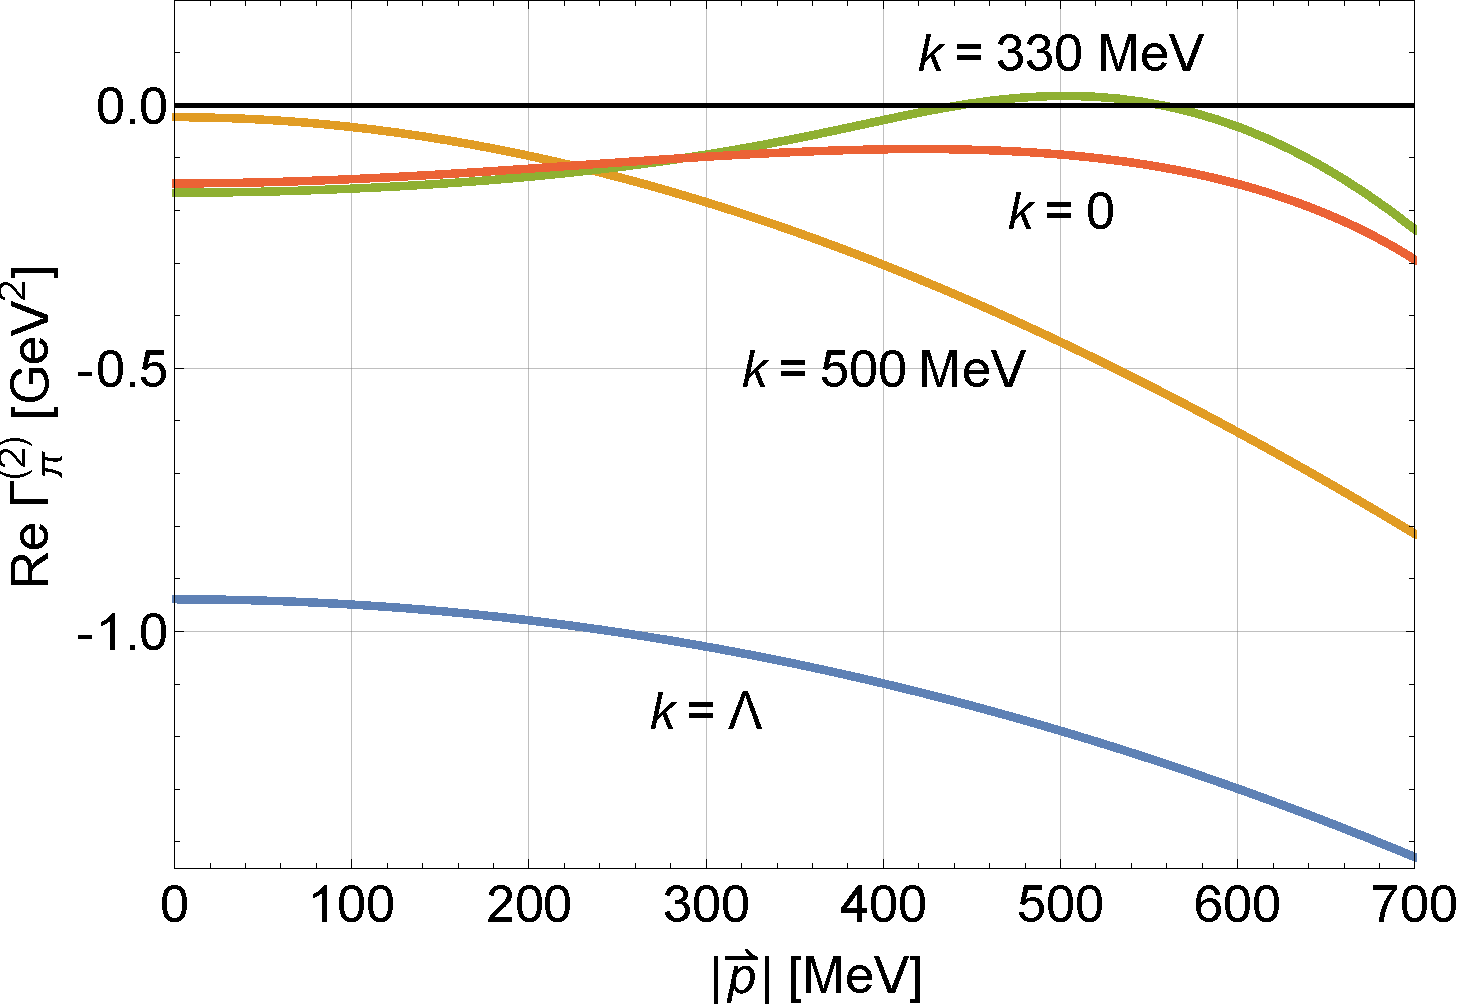
\includegraphics[width=\subcaptionFigureWidth+0.65cm]{inhomo/figures/PhysRevD.97.034022Fig5.pdf}} % left figure
	{\vspace{-0.15cm}\hspace{0.8cm}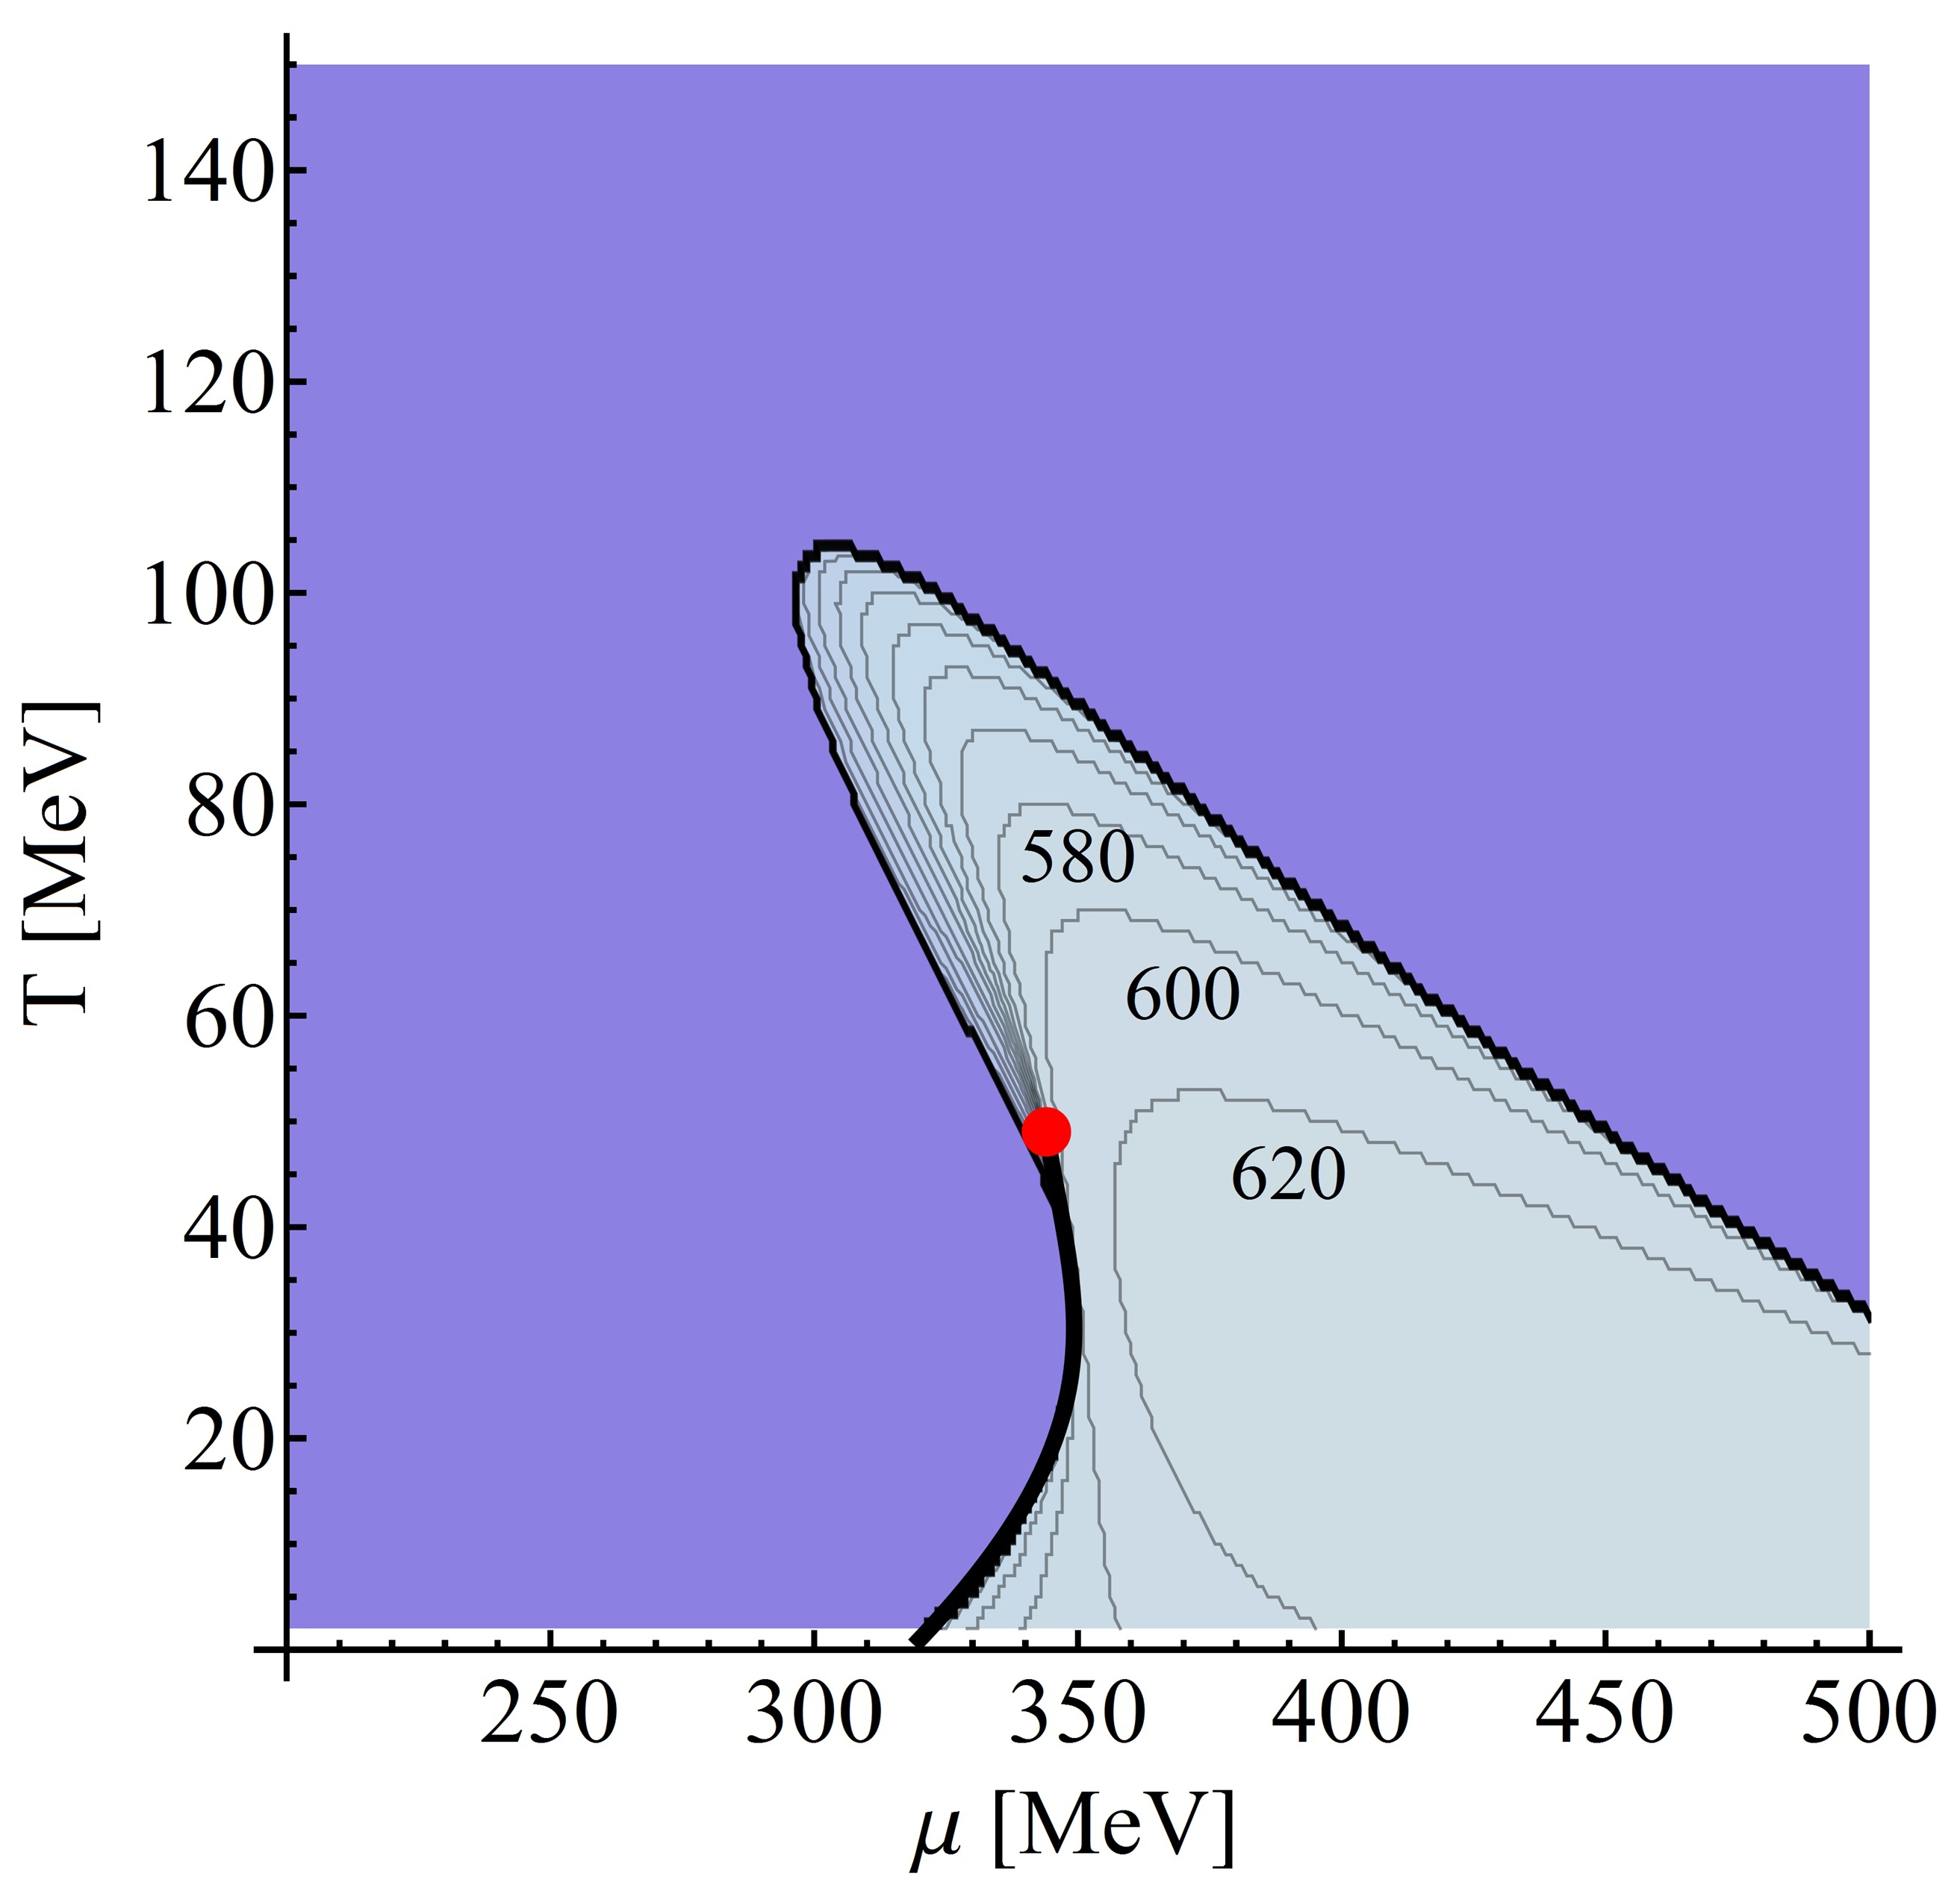
\includegraphics[width=\subcaptionFigureWidth-1.3cm]{inhomo/figures/PhysRevD.97.034022Fig6.png}} % Right figure
	[fig:QMMarno1,fig:QMMarno2]
	{%
		Results~\cite{Tripolt:2017zgc} from an \frg{} stability analysis in \lpa{} for the \qmm{}.
		On the left \subref{fig:QMMarno1} the static pion two-point function is shown for $\mu=400\,\MeV$ and $T=15\,\MeV$ at various \rgscales{} $k$.
		The zero crossings at $k=330\,\MeV$ are attributed to an instability of the homogeneous phase.
		On the right \subref{fig:QMMarno2} the region in the $\mu$-$T$-plane is marked where and when during the \frg{} flow such an instability occurs.
		\textit{Taken from the arXiv sources for Fig. 5 and 6 of \ccite{Tripolt:2017zgc} but for the presentation here we changed the location of the axes labels in the latter using Photoshop CS6~\cite{photoshopCS6}.}
		\ccbysaLicense{R.-A. Tripolt}
	}%
	{fig:QMMarno}

% ****** Models in zero dimensions ****** %
\chapter{Models in zero dimensions}\label{chap:zeroONSU2}\IMRADlabel{results}
\begin{disclaimer}
	Large parts of this chapter are based on \ccite{Koenigstein:2021syz,Koenigstein:2021rxj,Steil:2021cbu,Steil:partIV,Koenigstein:fixedPoint}.
	The individual sections include more detailed disclaimers.
	The involved collaborators are A. Koenigstein, N. Wink, E. Grossi, J. Braun, M. Buballa, and D. H. Rischke. 

	\Ccite{Koenigstein:2021syz,Koenigstein:2021rxj,Steil:2021cbu} are published manuscripts and parts of a series discussing zero-dimensional \ON{} models in the context of the \frg{}. The discussed research is also part of the dissertation~\cite{Koenigstein:2022phd} of A. Koenigstein. Most symbolic calculations, all numerical computations, and the majority of these manuscripts have been prepared by A. Koenigstein and me in equal shares. The other co-authors have been primarily involved in the conceptualization, discussion, and the finishing of the manuscripts.
		
	\Ccite{Steil:partIV} is an unpublished manuscript draft, which has been planed as a continuation and supplement to the series on \frg{} in zero dimensions.
	\Ccite{Koenigstein:fixedPoint} are unpublished notes on fixed-point solutions in the context of \ccite{Koenigstein:2021rxj}.
	
	The following introduction of this chapter has been compiled from the introductions and abstracts of \ccite{Koenigstein:2021syz,Koenigstein:2021rxj,Steil:2021cbu,Steil:partIV}.
\end{disclaimer}

We begin the main part of this thesis with the detailed discussion of our research regarding theories in zero space-time dimensions.
As demonstrated beautifully by Jan Keitel and Lorenz Bartosch with their work~\cite{Keitel:2011pn} and by numerous other authors, see, \eg{}, \ccite{\zerodRefs}, zero-dimensional theories are by no means trivial.
While it is true that they are easily solvable by just computing simple, ordinary integrals, their treatment within perturbative and non-perturbative methods employed in \qft{} is non-trivial.
Applying the \frg{}, \dses{}, nPI techniques, $\tfrac{1}{N}$-expansion schemes, and/or perturbative methods to zero-dimensional theories can be very illuminating.
Not only academic and didactic insights can be gained, but also deep conceptual and methodological developments are indeed possible with such studies.\bigskip 

As outlined in the introduction~\ref{paragraph:introZeroD}, the main purpose of the following discussions of this chapter is twofold.
\begin{enumerate}
	\item Using zero-dimensional theories, we want to gain academic, didactic, and conceptual insight into the \frg{} framework.
	\item Making use of the unique properties of \qfts{} in zero dimensions, we want to adapt and benchmark numerically stable methods for the solution of \frg{} flow equations.
\end{enumerate}
To achieve these goals we will apply and adapt methods from the field of \cfd{}, which we introduced in \cref{sec:conservationLaws}, to the \frg{}, which we introduced in \cref{sec:FRG}.

Zero-dimensional \qfts{} are uniquely well suited for such discussions, since the functional flow equations encountered in the \frg{} manifest directly as \pdes{} in zero dimensions.
It is possible to study the \frgEq{} and the related flow \cref{eq:dWkdtflow,eq:dZkdtflow} for $W_k[\FSff{J}]$ and $Z_k[\FSff{J}]$ directly, \ie{}, without the need of any truncations or approximations.
The flow equations can be readily expressed as conservation laws, allowing for a direct adaptation of concepts and methods from the field of \cfd{} to \frg{}.
Applications in zero dimensions make the somewhat vague notion of functional flow equations explicit as flow equations for functions. 
This supports and extends on the findings~\cite{Grossi:2021ksl} of Eduardo Grossi and Nicolas Wink and firmly establishes the very explicit notion of \frg{} flow equations as flow equations in a fluid-dynamical sense.
The exact flow equations encountered in zero dimensions share many crucial qualitative and, to an extent, even quantitative features with flow equations encountered in non-zero dimensions.
As such, our research and development in zero dimensions is far more than just an academic exercise, since it is very relevant and to a significant extent directly applicable in non-zero dimensions.\bigskip

We begin this chapter with a detailed discussion of zero-dimensional \qft{} using the $O(1)$ model of a single scalar as an instructive example in \cref{sec:0dQFT}.
We discuss general peculiarities of such \qfts{} in a single space-time point, but then shift focus especially on the manifestation of \frg{} in zero dimensions.
The \frg{} can be understood very intuitively  as an integral deformation \dash{} making the underlying idea of Wilson's \rg{} approach and the governing equations very tangible.
We retrace the general derivation of the \frgEq{} of \cref{sec:FRG} in zero-dimensions commenting in detail on the involved subtleties.
The fact that this discussion is based on functions and integrals instead of functionals and functional integrals allows for a simpler, but at the same time in many regards more concise discussion.\bigskip

In \cref{sec:0dON} we extend our discussion to zero-dimensional $O(N)$ models, where we allow for condensation in one radial direction leading to one massive \sigmaMode{} and $(N-1)$ \pionModes{}.
We use this model to study $O(N)$ symmetry restoration, by studying the \frg{} flow for various initial conditions/actions.
Basic symmetries of the underlying integrals prevent symmetry breaking in the \ir{} in zero dimensions.
This can be seen as an extreme limiting case of the \cmwhTheoremWithRefs{}, \cf{} \MWApp{}.

We will discuss the \frg{} flow evolution equation for the zero-dimensional $O(N)$ model at length.
Starting by casting it in conservative form, we continue to discuss initial conditions, boundary conditions, \rgcy{}, and irreversibility at length.
The conservative formulation allows for an identification of the \sigmaMode{} as diffusive contribution and of the \pionModes{} as advective contributions.

In \cref{subsec:0dONresults} we construct a series of test cases (initial conditions/actions) in the zero-dimensional $O(N)$ model at finite $N$.
For our explicit numerical computations  with the \frg{} flow equation, we adopt the \kt{} scheme of \cref{subsec:hydroKT} as our finite volume method of choice.
We discuss the advective and diffusive nature of \frg{} flows in detail using explicit numerical computations.
The impact of initial scales in the context of \rgcy{}, boundary conditions, and discretization in field space is discussed at length.
We also discus the, as it turns out rather limited, applicability of the \frg{} Taylor expansion as a possible truncation scheme in zero dimensions.

After our discussions of various finite $N$ results, we focus on the limiting cases $N=1$ and $N\rightarrow\infty$ in \cref{subsec:0dO1Entropy} and \cref{subsec:0dLargeN} respectively.
The focus of our discussion of the purely diffusive system at $N=1$ is the irreversibility of \grg{} flows from a \cfd{} perspective and the associated concept of (numerical) entropy.
A connection between the later and the concept of $\mathcal{C}$-/$\mathcal{A}$-functions is also discussed.
At large $N$ and ultimately in the limit $N\rightarrow\infty$ we study advection dominated and in the limit ultimately purely advective systems. 
The focus here are limitations of the large-$N$ saddle-point approximation and related \frg{}/\cfd{} concepts.
For our discussion we construct yet another test case, which we study using both numeric and analytic methods.
Shocks and rarefaction waves and their implications for the large-$N$ limit are discussed, including again comments on the irreversibility of \grg{} flows in such scenarios.\bigskip

In the penultimate \cref{sec:0dSU2} of this chapter we discuss Grassmann numbers as zero-dimensional analogs to fermions.
We present a $SU(2)$ model including two pairs of associated Grassmann numbers and three scalars, which we constructed as a zero-dimensional analog to the \qmm{}.
We discuss the model and the involved flow equations and comment at length on our plans for further research with such theories.
Compared to our, for the most parts, complete discussion of scalars in zero-dimensions, this work on Grassmann numbers is in a very early state.\bigskip

In \cref{sec:0dconclusion} we summarize our key research results of our extensive studies in zero dimensions and give an outlook for even further research with zero-dimensional \qfts{}.
Especially zero-dimensional models involving Grassmann numbers are identified as a very interesting and relevant area for further research.
\section{Quantum \texorpdfstring{\xcancel{field}}{(field)} theory in zero dimensions}\label{sec:0dQFT}
\begin{disclaimer}
	This section follows the discussion presented in Sec. II of \ccite{Koenigstein:2021syz}.
\end{disclaimer}
This section provides an introduction to zero-dimensional \qft{} using the theory of a single scalar as an instructive example.
We will focus on details and structure of the flow equations and the technical subtleties in their solution in zero dimensions thus without any direct reference to regularization and renormalization.
In addition we use this introduction to establish some notation and special features of zero-dimensional field theory.\\

As already mentioned in the introduction to this chapter, the efficient and sufficiently precise calculation of correlation functions is key to understanding the properties of a particular model or theory.
Usually this is done by introducing a partition function or functional integral that provides a probability distribution for the microstates of the model and serves as a generating functional for the $n$-point (correlation) functions~\cite{Weinberg:1996kr,Peskin:1995ev,ZinnJustin:2002ru,Kleinert:2004ev}.
The partition function is based on an energy function that can be a discrete or continuous Hamilton function or an action, which determines the microscopic properties of the model, \cf{} \cref{eq:ZkDef}.
The \frg{} provides an alternative to a direct computation using the functional integral.
For generic \qfts{} we introduced this approach in \cref{sec:FRG} but in this section we want to focus on the special case of a zero-dimensional \qft{} of a single scalar.
We will discuss the direct computation of observables using the generating functional and the alternative approach using the \frg{} flow equation.

\subsection{The partition function}\label{subsec:partition_function}
Consider a zero-dimensional \qft{} with a single real bosonic scalar field $\phi$\footnote{
Throughout this chapter we will use $\phi$ denote a fluctuating scalar (not $\FSff{\phi}$) since we will use $\varphi$ for the expectation value $\langle \phi\rangle=\varphi$.
Later in \cref{sec:0dSU2}, we will also introduce $\Ftheta$ and $\Fthetab$ as fluctuating Grassmann numbers with the corresponding expectation values $\langle\Ftheta\rangle=\MFtheta$ and $\langle\Fthetab\rangle=\MFthetab$.
Sadly variant versions are not available for all Greek characters, which led us to introduce the tilde-overline in our general discussion of \cref{sec:FRG}.
}.
In zero dimensions the ``field'' $\phi$ is due to the complete absence of a notion of space-time in zero dimensions mathematically not a field but just a single scalar degree of freedom, \ie{}, a plain real number \dash{} hence the typographic pun with striking out the word \textit{field} in the title of this section.
In our following discussion we will however maintain the term field even though mathematically we are just discussing numbers.
Due to the absence of space-time in zero dimensions derivatives and space-time integrals simply do not exist.
This implies that the action $\mathcal{S}[\phi]$ of the model is identical to the Lagrangian $\mathcal{L}[\phi]$.
The action, the Lagrangian, and also the Hamiltonian $\mathcal{H}[\phi]$ are simply functions of $\phi$ instead of functionals%
\footnote{%
	Nevertheless, we will stick to the notation of functionals using square brackets, to maintain a degree of consistency with the corresponding expressions in non-zero space-time dimensions, as long as we do not focus on particular zero-dimensional examples.
}.
The complete absence of space-time derivatives/integrals, fields, and functionals makes the following discussion mathematically rather simple in stark contrast to the situation encountered by \qft{} practitioners in $d>0$: where dealing with potentially divergent space-time integrals and complicated functional integrals is the norm.
This simplicity is the beauty of zero-dimensional \qfts{} which are by no means trivial: a lot can be learned from their study.
Because of the absence of a space-time derivative and thus of kinetic terms, $\mathcal{S}[\phi] = \mathcal{L}[\phi] = \mathcal{H}[\phi] = U(\phi)$, where $U(\phi)$ is the (effective) potential.
Therefore, the only requirement for these functions is that they must be bounded from below, in order to exclude ``negative-energy states''%
\footnote{
	We put ``negative-energy states'' in quotation marks, because all quantities in zero-dimensional field theory are dimensionless, \viz{} bare numbers without physical dimensions.
	For convenience, we will still use the well-established notions from higher-dimensional \qfts{} in our discussion.
}
and to obtain positive normalizable probability distributions.
Apart from this requirement, for the moment we do not demand any additional properties, like symmetries (\eg{}, \ZII{}, $\phi \rightarrow - \phi$) or analyticity.

If we choose a specific model with action $\mathcal{S}[\phi]$ all expectation values of arbitrary functions $f(\phi)$ that do not grow exponentially in $\phi$ are defined and can be calculated via the following expression
\begin{align}
	\langle f(\phi) \rangle \equiv \frac{\int_{-\infty}^{+\infty} \dif \phi \, f(\phi) \, \eu^{ - \mathcal{S}[\phi] }}{\int_{-\infty}^{+\infty} \dif \phi \, \eu^{ - \mathcal{S}[\phi] }} \, ,	\label{eq:expectation_value_1}
\end{align}
where $\eu^{ - \mathcal{S}[\phi] }$ provides the partition of probabilities among the microstates.
Note that due to the zero-dimensional nature all expectation values for such a model reduce to indefinite one-dimensional integrals over $\phi$.
Such integrals can be computed to extremely high precision using standard techniques of numerical integration~\cite{Press:1992zz,PresTeukVettFlan92}.
It is worth emphasizing that the current discussion holds also for non-analytic $\mathcal{S}[\phi]$ and/or $f(\phi)$.
Some specific choices of $\mathcal{S}[\phi]$ and $f(\phi)$ even allow for an analytic evaluation of \cref{eq:expectation_value_1}, see, \eg{}, \ccite{Keitel:2011pn}.
The possibility to compute expectation values to high precision makes zero-dimensional field theory of great interest as a testing ground for approximations and/or numerical methods.

Some explicit examples of zero-dimensional field theories used as a testing ground for methods in statistical mechanics and \qft{} can be found in \ccite{Bessis:1980ss,Zinn-Justin:1998hwu,DiVecchia:1990ce,Hikami:1978ya,Nishigaki:1990sk,Schelstraete:1994sc,Keitel:2011pn,Pawlowski:talk,Moroz:2011thesis,Fl_rchinger_2010,SkinnerScript,Strocchi:2013awa,Kemler:2013yka,Rentrop_2015,Rosa:2016czs,Liang:2017whg,Millington:2019nkw,Alexander:2019cgw,Catalano:2019,Millington:2020Talk,Millington:2021ftp,Kades:2021hir,Fraboulet:2021amf}.
In \ccite{Strocchi:2013awa}, for example, the asymptotic convergence and the vanishing convergence radius of perturbation theory of $\phi^4$-theory is discussed.
Approximation schemes such as the large-$N$, the \frg{} vertex expansion, or the \frg{} Taylor expansion were analyzed in \ccite{Keitel:2011pn}.
Zero-dimensional field theory was also used to study density-functional theory in \ccite{Kemler:2013yka,Rentrop_2015,Liang:2017whg} and applied to fermionic fields in \ccite{SkinnerScript}.
Recently, it was used to study and visualize 2PI effective actions~\cite{Millington:2019nkw} \dash{} also in the \frg{} framework~\cite{Alexander:2019cgw,Millington:2020Talk,Millington:2021ftp}.

The calculation of expectation values is facilitated by a suitably defined generating functional
\begin{align}
	\mathcal{Z} [J] \equiv \mathcal{N} \int_{-\infty}^{+\infty} \dif \phi \, \eu^{- \mathcal{S}[\phi] + J \, \phi} \, , \label{eq:partition_function}
\end{align}
from which one can derive all correlation functions by taking the corresponding number of derivatives \wrt{} the external source $J$,
\begin{align}
	\langle f(\phi) \rangle = \frac{f(\tfrac{\delta}{\delta J}) \, \mathcal{Z}[J]}{\mathcal{Z}[J]} \bigg|_{J = 0} \, .	\label{eq:expectation_value_2}
\end{align}
One should note that if $f(\phi)$ is non-analytic, then \cref{eq:expectation_value_2} is to be understood symbolically.
Otherwise, it is defined through a Taylor series in $\frac{\delta}{\delta J}$.
Irrespective of that, \cref{eq:expectation_value_1} and \eqref{eq:partition_function} are always well defined and \cref{eq:partition_function} can be always calculated for arbitrary $J$.
One can even show in zero dimensions that $\mathcal{Z}[J] \in C^\infty$, hence, $\mathcal{Z}[J]$ is a smooth function, see \ccite{Moroz:2011thesis} and \MWApp{}.

The normalization $\mathcal{N}$ is not an observable quantity and for our discussion here, it is convenient to choose
\begin{align}
		\mathcal{Z} [ 0 ] \overset{!}{=} 1 \qquad \longleftrightarrow \qquad \mathcal{N}^{-1} = \int_{-\infty}^{+\infty} \dif \phi \, \eu^{ - \mathcal{S} [\phi] } \, .	\label{eq:normalization}
\end{align}
As already mentioned above, calculating expectation values in a zero-dimensional \qft{} via \cref{eq:expectation_value_1} is (at the very least numerically) rather straightforward.
In contrast, for higher-dimensional models or theories with non-trivial field content, calculating functional integrals similar to \cref{eq:expectation_value_1}, \cf{} \cref{eq:expectationOJ}, with sufficient precision is usually extremely challenging or might even be impossible with limited computational resources.
Therefore, alternative methods like the \frg{} or approximation schemes apart from ``direct numerical integration'', like in lattice simulations, are of great interest.

In the following, we will again focus on the \frg{} as a specific method for calculating \nptFunctions{} in zero-dimensional \qfts{}.
In contrast to the usual motivation of the \frg{}, \cf{} the introduction of \cref{sec:FRG}, we will use a different but as it turns out closely related approach to motivate and ultimately arrive at the \frg{} flow equation \eqref{eq:WetterichEq0d} in zero-dimensions.
To this end, we will follow and extend the discussion in \ccite{Keitel:2011pn,Pawlowski:talk,Moroz:2011thesis,Fl_rchinger_2010,SkinnerScript} and discuss its technical properties as an alternative way of solving the integrals in \cref{eq:expectation_value_1} and \eqref{eq:partition_function}.

\subsection{Solving integrals with flow equations}\label{subsec:0dintegrals}
The starting point of our following discussion, is the observation that there is one well-known non-trivial class of actions $\mathcal{S}[\phi]$ for which the calculation of integrals like \cref{eq:expectation_value_1} is straightforward, even in higher dimensions and even for more complicated field content.
These actions are \qfts{} for ``(massive) free particles'' and correspond to Gaussian-type integrals.
In the present case the Gaussian-type action takes the following simple form,
\begin{align}
	\mathcal{S} [ \phi ] = \tfrac{m^2}{2} \, \phi^2 \, .	\label{eq:mass_term}
\end{align}
where $m$ is called a ``mass'' for convenience, although it is actually a dimensionless quantity in zero space-time dimensions.

For non-trivial actions $\mathcal{S}[\phi]$, \cref{eq:expectation_value_1} can still be approximated by a Gaussian integral, as long as $\mathcal{S}[\phi]$ contains a mass term \eqref{eq:mass_term} with a coefficient $m^2$ that is much larger than all other scales contained in $\mathcal{S}[\phi]$.
If this is the case, the Gaussian part of the integrand $\eu^{-\mathcal{S}[\phi]}$ completely dominates the integrals in \cref{eq:expectation_value_1} and \eqref{eq:partition_function}.
The reason is that the mass term $\sim\phi^2$ is dominant for small and moderate $\phi$, and most of the area under the curve $\eu^{-\mathcal{S}[\phi]}$ lies in the region of small $\phi$, similar to a pure Gaussian integral.
For very large values of $\phi$ other terms in the action $\mathcal{S}[\phi]$ may become more important.
Nevertheless, if $m^2$ is large enough, the corresponding area under the curve $\eu^{-\mathcal{S}[\phi]}$ is completely negligible in regions where $\phi$ is large, because $\mathcal{S}[\phi]$ is bounded from below such that $\eu^{-\mathcal{S}[\phi]}$ tends to zero exponentially fast for $\phi\to\infty$.
In summary, the Gaussian part with the huge mass term dominates the integral and even integrals involving non-trivial actions can be approximated.
This is illustrated in \cref{fig:rg_flow_integrand}.

\subsubsection{The scale-dependent partition function}
Based on the above observation, let us now (re)introduce the following quantity:
\begin{align}
	\mathcal{Z}_t [ J ] \equiv \mathcal{N} \, \int_{-\infty}^{+\infty} \dif \phi \, \eu^{- \mathcal{S} [ \phi ] - \Delta \mathcal{S}_t [ \phi ] + J \, \phi } \, ,	\label{eq:scale_dependent_z}
\end{align}
which is called the \textit{scale-dependent generating functional} or \textit{scale-dependent partition function}.
It differs from the usual partition function \eqref{eq:partition_function} only by a scale-dependent mass term
\begin{align}
	\Delta \mathcal{S}_t [ \phi ] \equiv \tfrac{1}{2} \, r ( t ) \, \phi^2 \, .	\label{eq:regulator_insertion}
\end{align}
We directly adopt the common notation from the \frg{} community and call $r(t)$ the \textit{regulator (shape) function}, which depends on the \textit{\rgscale{}} (``\textit{time}'') $t \in [ \, 0 , \infty )$, see, \eg{}, \ccite{Litim:2000ci,Pawlowski:2015mlf}.
We have now constructed the zero-dimensional analog to the \rgscaledependent{} generating functional \eqref{eq:ZkDef} purely based on the notion of an integral deformation.
For now, we only demand that the function $r(t)$ has such properties that $\mathcal{Z}_t [J]$ interpolates between an almost Gaussian-type partition function%
\footnote{%
	This is also why the \uv{} fixed point of \grg{} flows is denoted as the \textit{trivial} or \textit{Gaussian fixed point}.
}
with extremely massive free fields at $t = 0$ and the actual partition function $\mathcal{Z}[J]$ of interest at $t \rightarrow \infty$.
In order to achieve this behavior, $r ( t )$ has to have the following properties:
	\begin{enumerate}
		\item	In the limit of $t \rightarrow 0$, $r(t)$ ($\Delta \mathcal{S}_t [ \phi ] $) should behave like a mass (term), similar to what we discussed at the beginning of this section, and be much larger than all other scales in $\mathcal{S}[\phi]$. We will discuss this further in \cref{subsec:exact_rg_equation}.
		
		\item	For $t \rightarrow \infty$, $r(t)$ is supposed to vanish, such that $\lim_{t \rightarrow \infty} \mathcal{Z}_t [J]=\mathcal{Z}[J]$.
		The same applies to expectation values calculated from $\mathcal{Z}_t[J]$, which become expectation values of $\mathcal{Z}[J]$.
		For practical calculations it is sufficient to assume that, for $t \rightarrow \infty$, $r(t)$ becomes much smaller than all scales in $\mathcal{S}[\phi]$, because then the contribution $\Delta \mathcal{S}_t [\phi]$ to the whole integrand $\eu^{- \mathcal{S}[\phi] - \Delta \mathcal{S}_t [\phi]}$ is negligible and the integrand is almost identical to $\eu^{- \mathcal{S}[\phi]}$.
		The value $\lim_{t \rightarrow \infty} r ( t ) = r_\mathrm{IR} \smallergtrsim 0$ is usually referred to as \textit{(numerical) \ir{} cutoff}.
		
		\item	The interpretation of $r(t)$ ($\Delta \mathcal{S}_t [ \phi ]$) as a mass (term) is guaranteed by further demanding monotonicity, ${\forall t,\ \partial_t r(t) \leq 0}$.
		We will provide additional arguments for monotonicity in \cref{subsec:flow_equation_of_the_partition_function}.
				
		\item	In order to be able to smoothly deform the integral in \cref{eq:partition_function} and for the following derivation of evolution equations, we further require $r ( t ) \in C^1$.
	\end{enumerate}
Apart from these four properties there are no further requirements on $r(t)$ in zero dimensions and ultimately the regulator choice in zero-dimensions manifests as simple reparametrizations in the flow time $t$.
The first (\uv{}) property is the zero-dimensional realization of general regulator property \customref{paragraph:regulatorUV}{3. \textit{Diverging in the Ultraviolet}} of \cref{subsubsec:regulator}.
The second (\ir{}) property is the zero-dimensional realization of general regulator property \customref{paragraph:regulatorHighP}{2. \textit{Vanishing for high momentum modes}} of \cref{subsubsec:regulator}.
Note that for higher-dimensional field theories the fourth requirement turns into $\Delta \mathcal{S}_t [ \phi ] \in C^1$.
A specific choice which is used in large parts of our work is the zero-dimensional exponential regulator (shape) function
	\begin{align}
		r ( t ) = \Lambda \, \eu^{- t} \, ,	\label{eq:exponential_regulator}
	\end{align}
with an \uv{} cutoff/scale $\Lambda$, which must be chosen much larger than all scales in $\mathcal{S} [ \phi ]$.

In order to get a better intuition of the effect of $r(t)$ on the integral \eqref{eq:scale_dependent_z}, we show the integrand at $J=0$, $\eu^{- \mathcal{S}[\phi] - \Delta \mathcal{S}_t [\phi]}$, and the respective exponent for different values of $t$ for the analytic action
\begin{align}
	\mathcal{S} ( \phi ) = - \tfrac{1}{2} \, \phi^2 + \tfrac{1}{4!} \, \phi^4 \, ,\label{eq:example_analytic_action}
\end{align}
in \cref{fig:rg_flow_integrand_z_1} and in \cref{fig:rg_flow_integrand_z_2} the same quantities for the non-analytic action
	\begin{align}
		\mathcal{S} ( \phi ) =
		\begin{cases}
			- \phi^2 \, ,								&	\text{if} \quad | \phi | \leq \tfrac{5}{4} \, ,	
			\\[.1em]
			- \big( \tfrac{5}{4} \big)^2 \, ,			&	\text{if} \quad \tfrac{5}{4} < | \phi | \leq 2 \, ,
			\\[.1em]
			\tfrac{1}{48} \,, \big( \phi^4 - 91 \big)	&	\text{if} \quad | \phi |>2 \, .
			\\
		\end{cases}	\label{eq:example_non-analytic_action}
	\end{align}
The figures show how the integrands are deformed from Gaussian-shaped integrands to the integrands $\eu^{- \mathcal{S}[\phi]}$.
One observes that, as long as $r(t)$ is much larger than all other parameters in $\mathcal{S}[\phi]$, the Gaussian-like mass term dominates, while for increasing $t$ the regulator $r(t)$ becomes negligible.
The most interesting part, where the integrands change their shapes significantly, is where $r(t)$ is of the same order as the scales in $\mathcal{S} ( \phi )$.
\subcaptionFigure%
	[t]% Placement
	{0d/figures/rg_flow_integrand_z_smooth.pdf}% Figure (a)
	[\captionsetup{justification=centering}\caption{Plots for the action \eqref{eq:example_analytic_action}}]% Caption (a)
	{fig:rg_flow_integrand_z_1}% label (a)
	{0d/figures/rg_flow_integrand_z_kink.pdf}% Figure (b)
	[\captionsetup{justification=centering}\caption{Plots for the action  \eqref{eq:example_non-analytic_action}}]% Caption (b)
	{fig:rg_flow_integrand_z_2}% label (b)
	{%
	The integrand (upper panel) and exponent (lower panel) from \cref{eq:scale_dependent_z} (at $J = 0$) as a function of the field variable $\phi$ for various \rgtimes{} $t = 0, 1, 2, \ldots, 15$ and for different actions on the left \subref{fig:rg_flow_integrand_z_1} and on the right \subref{fig:rg_flow_integrand_z_2}.
	We choose the exponential regulator~\eqref{eq:exponential_regulator} with \uv{} scale $\Lambda = 10^3$.
	The \ir{} cutoff scale is chosen at  $r_\mathrm{IR} \simeq 3.06 \cdot 10^{-4}$ which corresponds to $t = 15$.
	The numerical value of $r_\mathrm{IR}$ is significantly smaller than all scales in $\mathcal{S}[\phi]$.
	\fromFigs{1 and 2}{zerod1}%
	}% Caption
	{fig:rg_flow_integrand}% Label

\FloatBarrier
\subsubsection{A flow equation for the scale-dependent partition function}
\label{subsec:flow_equation_of_the_partition_function}

The change of the integrals with $t$ between the two limiting cases at $t=0$ and $t\rightarrow\infty$ is the in \cref{sec:FRG} established \textit{\frg{} flow} from the \uv{} to the \ir{}.
By knowing/mathematically prescribing the integral deformation, we can obtain the function ${\mathcal{Z}(J) \equiv \lim_{t \rightarrow \infty} \mathcal{Z}_t [J] = \mathcal{Z}[J]}$ right from the Gaussian-like partition function $\mathcal{Z}_{t = 0}[J]$ without the need to calculate the $\phi$-integral in the partition function~\eqref{eq:partition_function} directly.
In zero dimensions this might arguably be one of the most complicated ways to compute the partition function~\eqref{eq:partition_function}, because the integrals in field space are (at least numerically) simple to compute.
For higher dimensions, however, circumventing the corresponding challenging functional integration is a tremendous benefit.\bigskip

The \frg{} flow of $\mathcal{Z}_t [J]$, \ie{}, its deformation, is prescribed by a differential equation which can be obtained by taking the derivative \wrt{} the \rgtime{} $t$ of \cref{eq:scale_dependent_z}:
\begin{subequations}\label{eq:pde_zF}
\begin{align}
		\partial_t \mathcal{Z}_t[J] =	\, & - \big[ \tfrac{1}{2} \, \partial_t r ( t ) \big] \, \mathcal{N} \int_{-\infty}^{+\infty} \dif \phi \, \phi^2 \, \eu^{ - \mathcal{S}[\phi] - \Delta \mathcal{S}[\phi] + J \, \phi}\, =\\
		=\,& - \big[ \tfrac{1}{2} \, \partial_t r ( t ) \big] \, \frac{\delta^2 \mathcal{Z}_t [J]}{\delta J \, \delta J} \equiv \,  - \big[ \tfrac{1}{2} \, \partial_t r ( t ) \big] \, \mathcal{Z}^{(2)}_{t, J J} [J] \, ,	
	\end{align}
\end{subequations}
which directly manifests as a simple \pde{} for the function $\mathcal{Z} ( t, J )$ in the $t$-$J$-plane,
\begin{align}
	\partial_t \mathcal{Z}(t,J) = - \big[ \tfrac{1}{2} \, \partial_t r ( t ) \big] \, \partial_J^2 \mathcal{Z}(t,J) \, .	\label{eq:pde_z}
\end{align}
Solving this equation with appropriate initial and boundary conditions results in a function $\mathcal{Z} ( J )$ from which one can calculate expectation values by taking ordinary (numerical) derivatives \wrt{} $J$ at $J = 0$, \cf{}\ \cref{eq:expectation_value_2}.

The higher-dimensional analog to \cref{eq:pde_z} is \cref{eq:dZkdtflow} and thus we again recognize \cref{eq:pde_z} as a linear one-dimensional diffusion equation (\textit{heat equation})~\cite{Rosten:2010vm,SkinnerScript,Salmhofer:2020Talk,Cannon:1984}, where $t$ corresponds to the temporal direction, while $J$ corresponds to the spatial direction.
We discussed this type of conservation equation in detail in \cref{subsec:hydroDiffusion}.
The term $- \tfrac{1}{2} \, \partial_t r ( t )$ corresponds to a time-dependent (positive definite) diffusion coefficient%
\footnote{%
	Note that in zero dimensions one can get rid of $\partial_t r ( t )$ by an appropriate reparametrization of the time coordinate $t$, which nevertheless keeps the structure of the equation unchanged.
	In higher dimensions this elimination of $r ( t )$ is in general not possible.
	The positivity of the diffusion coefficient is directly related to the stability of solutions of the heat equation~\cite{LeVeque:1992,LeVeque:2002} and positivity \dash{} here guaranteed by the regulator properties \dash{} is necessary for a stable solution~\cite{Rosten:2010vm,Osborn:2011kw}.
}.
This further supports the notion of \rg{} ``time'' for the parameter $t$.
We will come back to the concept of \rg{} ``time'' in the true sense of the word and the diffusive, irreversible character of \frg{} flows in \cref{subsubsec:conservative_form}.\bigskip

For the remainder of this subsection we will discuss properties and practical issues considering the exact \pde{} \eqref{eq:pde_z}.
We will neither discuss any kind of expansions in $J$ nor its application in higher dimensions here.
However, some of the issues and questions raised in the following are also relevant for higher-dimensional theories.

Finding the correct initial and boundary conditions for numerical solutions of \cref{eq:pde_z} as an exact \pde{} is challenging.
By construction $\mathcal{Z}_{t = 0} [ J ]$ approaches a Gaussian integral,
\begin{align}
	\stepcounter{equation}\newSubEqBlock
	\mathcal{Z}_{t = 0} [ J ] = \, & \mathcal{N} \, \int_{-\infty}^{+\infty} \dif \phi \, \eu^{- \frac{1}{2} r ( 0 ) \, \phi^2 + J \, \phi} \, \eu^{- \mathcal{S} ( \phi )}\,=\subEqTag\\* % no page break
	= \, & \mathcal{N} \, \int_{-\infty}^{+\infty} \frac{\dif\tilde{\phi}}{\sqrt{r(0)}} \, \eu^{- \frac{1}{2} \, \tilde{\phi}^2 + J \, \frac{\tilde{\phi}}{\sqrt{r(0)}}} \, \Big[ 1- \order \big( \mathcal{S} \big( r ( 0 )^{-\frac{1}{2}} \big) \big) \Big]\,= \subEqTag\\* % no page break
	= \, & \mathcal{N} \, \sqrt{\tfrac{2\piu}{r(0)}} \, \eu^{\frac{J^2}{2 r(0)}} \, \Big[ 1- \order \big( \mathcal{S} \big( r(0)^{-\frac{1}{2}} \big) \big) \Big] \, ,	\label{eq:initial_condition_z}
\end{align}
with $\tilde{\phi}\equiv \sqrt{r(0)}\,\phi$ and independent of the explicit shape of $\mathcal{S}[\phi]$.
Considering different actions $\mathcal{S}[\phi]$ with couplings of the same order of magnitude we can choose the same regulator with an $r(0)$ larger than all internal scales involved in the different actions.
The \ic{} $\mathcal{Z}(0,J)$ is then independent of the explicit action under consideration.

According to the integral formulation~\eqref{eq:scale_dependent_z}, $\mathcal{Z}(t,J)$ changes for different actions when $t > 0$.
In the differential formulation of the \cref{eq:pde_z} those changes are generated by the diffusion term on the \rhs{}
However, we argued that it is permissible to use identical \ics{} $\mathcal{Z} ( 0, J)$ for different actions involving similar scales (as long as these are much smaller than $r ( 0 )$).
This then results in an identical diffusion on the \rhs{} of \cref{eq:pde_z} when the latter is computed by means of a second derivative of $\mathcal{Z}(0,J)$.
If one uses identical large-$J$ \bcs{} for the solution of the \pde{} \eqref{eq:pde_z} for different actions, this would imply that, despite different $\mathcal{S}[\phi]$, the \rgtime{} evolution leads to identical $\mathcal{Z}(J)$ for $t\rightarrow\infty$, which in general cannot be correct.

In order to resolve this problem, particular action-dependent spatial \bcs{} seem to be necessary for a direct numerical solution starting at $t = 0$ with a Gaussian for $\mathcal{Z} ( 0, J )$.
It is not obvious how to derive or formulate such \bcs{} from the asymptotics of \cref{eq:pde_z} alone.
In light of this, a numerical solution of \cref{eq:pde_z} in the $t$-$J$-plane by means of a spatial discretization in $J$-direction and an integration in $t$-direction in the spirit of \cref{subsec:hydroDiffusion} appears to be conceptually questionable.

However, this invalidates by no means the flow equation for $\mathcal{Z} ( t, J )$ in general.
Augmenting it (at $t = 0$) with information from the integral formulation~\eqref{eq:scale_dependent_z} or, equivalently, other additional information, could enable practical computations using the \pde{} \eqref{eq:pde_z}.
But it is at this point (at least to us) not obvious how one would implement a numerical solution strategy for the \pde{} \eqref{eq:pde_z} avoiding integrals of the action.\\

There is another well-known drawback in using the partition function $\mathcal{Z} [ J ]$ for calculating \nptFunctions{} (or expectation values) $\langle \phi^n \rangle$.
The latter are rather inefficient in storing information, because they contain redundant information in the form of disconnected and reducible terms, see \ccite{Iliopoulos:1974ur,ZinnJustin:2002ru,Weinberg:1996kr,Peskin:1995ev} or the mathematical theory of moment- and cumulant-generating functionals in statistics for details~\cite{McCullagh:2009}.
This is also discussed in Sec.~II.E of \nbccite{zerod1}.
However, the redundant information in $\langle \phi^n \rangle$ is not necessarily a strong argument against the use of the flow equation \eqref{eq:pde_z} in practical computations, since the irreducible information can be extracted from the correlation functions $\langle \phi^n \rangle$.\bigskip

\subsection{The functional renormalization group equation}\label{subsec:exact_rg_equation}
To resolve both the problem of initial and \bcs{} for $\mathcal{Z}(t,J)$ as well as the issue of redundant information in $\langle \phi^n \rangle$, we now consider two different generating functionals the \textit{scale-dependent Schwinger functional} in \cref{subsubsec:WtJd0} and the \textit{scale-dependent effective action} in \cref{subsubsec:scale_dependent_effective_action}. 
Especially the latter will turn out to be much better suited for practical calculations of correlation functions/expectation values.
In this subsection we will derive and discuss the \frg{} flow \cref{eq:WetterichEq0d} for our zero-dimensional toy model \qft{} by subsequently (re)discovering the zero-dimensional analogs to the general expressions of \cref{sec:FRG}.
	
\subsubsection{The scale-dependent Schwinger functional}
\label{subsubsec:WtJd0}
We begin our journey towards the \frg{} flow \cref{eq:WetterichEq0d} by introducing the \textit{scale-dependent Schwinger functional} starting from definition~\eqref{eq:scale_dependent_z},
\begin{align}
	\mathcal{W}_t [J] \equiv \ln \mathcal{Z}_t [J] \, ,	\label{eq:scale_dependent_w}
\end{align}
in direct analogy to \cref{eq:WkDef}.
It follows from our previous discussion that for $t \rightarrow \infty$ the Schwinger functional $\mathcal{W}[J] \equiv \ln \mathcal{Z}[J]$ with	$\mathcal{W} [ 0 ] = 0$ is recovered,
\begin{align}
	\lim\limits_{t \rightarrow \infty} \mathcal{W}_t [J] = \mathcal{W} [J] \, ,
\end{align}
while $\mathcal{W}_{t = 0} [J]$ is given by the logarithm of \cref{eq:initial_condition_z}.

In general $\mathcal{W}[J]$ is convex with a positive definite Hessian $\mathcal{W}^{(2)}_{J J} [ J ]$.
In the present case the convexity of $\mathcal{W} [ J ] = \mathcal{W} ( J )$ becomes apparent considering its second derivative,
\begin{align}
	\partial_J^2 \mathcal{W}(J) = \langle \phi^2 \rangle_J -\langle \phi \rangle_J \langle \phi \rangle_J= \langle (\phi-\langle \phi \rangle_J)^2\rangle_J \, ,	\label{eq:jacobian_w}
\end{align}
which, as the expectation value of a positive quantity, is always positive.
Note that also $\mathcal{Z}[J]$ is convex, which can be seen by investigating its second derivative.
In zero dimensions, also smoothness, \ie{}, $\mathcal{Z} [ J ] \in C^\infty$, directly translates to $\mathcal{W} [ J ] \in C^\infty$, because all moments of $\mathcal{W} [ J ]$ can be entirely expressed in terms of derivatives of $\mathcal{Z} [J]$, see Sec.~II.E of \nbccite{zerod1} for explicit expressions.
The insertion of the regulator \eqref{eq:regulator_insertion} into $\mathcal{Z}_t [J]$ does not spoil the convexity and smoothness (in zero dimensions) of the Schwinger functional: $\mathcal{W}_t [J]$ and $\mathcal{Z}_t [J]$ are convex and smooth for all $t$.

Completely analogous to \cref{eq:pde_zF} one can derive a \pde{} for $\mathcal{W}_t[J] = \mathcal{W}(t,J)$ in the $t$-$J$-plane,
\begin{align}
	\partial_t \mathcal{W}(t,J) =	\, - \big[ \tfrac{1}{2} \, \partial_t r ( t ) \big] \, \Big( \partial_J^2 \mathcal{W}(t,J) + \big[ \partial_J \mathcal{W}(t,J) \big]^2 \Big) \, .\label{eq:pde_w}
\end{align}
which describes the flow of $\mathcal{W}(t,J)$ from $t = 0$ to $t \rightarrow \infty$.
We have recovered the zero-dimensional analog to \cref{eq:dWkdtflow}.

We could now repeat the discussion about the issues of initial and boundary conditions for the solution of this \pde{}.
However, the problems are almost identical to those of \cref{eq:pde_z}, because on the level of the \pde{}, we only substituted the function $\mathcal{Z} ( t, J )$ by $\mathcal{W} ( t, J )$ via the logarithm, which does not change the structure of the problem fundamentally.
Formulating appropriate initial and boundary conditions in the spatial $J$-direction therefore remains as complicated as before.
Note that the \pde{} \eqref{eq:pde_w} is even more complicated when compared to \cref{eq:pde_z} due to the non-linear term on the right-hand side.
In summary, the scale-dependent Schwinger functional is, from a practical point of view, as badly suited as $\mathcal{Z}(t,J)$ to perform the (numeric) calculation of the functional integral via a flow equation starting from a Gaussian-type integral.

\subsubsection{The scale-dependent effective action}\label{subsubsec:scale_dependent_effective_action}
In the following we will focus on the scale-dependent effective (average) action and its respective flow equation.
We define the \textit{scale-dependent effective action} $\Gamma_t[\varphi]$ via the Legendre transform of \cref{eq:scale_dependent_w} \wrt{} the sources $J$ at a \rgtime{} $t$,
\begin{subequations}
\begin{align}
	\Gamma_t [\varphi] \equiv \, & \mathop{\mathrm{sup}}_J \big( J \, \varphi - \mathcal{W}_t[J] \big)\, ,\label{eq:scale_dependent_effective_action}\\
	\equiv  \, & J_t(\varphi) \, \varphi - \mathcal{W}_t[J_t(\varphi)] \, ,	\label{eq:scale_dependent_effective_action_Jt}
\end{align}
\end{subequations}
where we introduced the source $J_t(\varphi)$ which realizes the supremum.
Note that, analogous to $\mathcal{Z}_t [J]$ and $\mathcal{W}_t [J]$, the convexity and smoothness (in zero dimensions) of $\Gamma_t [\varphi]$ is not spoiled by the $t$-dependence, because the properties of the Legendre transformation still ensure both, since the Legendre transform of the convex function $\mathcal{W}_t[J]$ is convex by definition, see, \eg{}, \ccite{Fujimoto:1982tc,Wipf:2013vp} for details.
	
To obtain an explicit relation for the scale-dependent source $J_t ( \varphi )$, which realizes the supremum in \cref{eq:scale_dependent_effective_action}, we consider the functional derivative of \cref{eq:scale_dependent_effective_action} at the supremum to find the important relation
\begin{align}
	\mathcal{W}_{t,J}^{(1)}[J_t(\varphi)] \equiv \frac{\delta \mathcal{W}_t [J]}{\delta J}\bigg|_{J=J_t(\varphi)} = \varphi \, ,	\label{eq:definition_phi_t}
\end{align}
which will be used frequently in the following.
Taking the functional derivative of \cref{eq:scale_dependent_effective_action_Jt} \wrt{} $\varphi$ and using \cref{eq:definition_phi_t} we ultimately rediscover the \textit{quantum equation of motion} in zero-dimensions:
\begin{align}
	\Gamma^{(1)}_{t, \varphi}[\varphi] \equiv \frac{\delta \Gamma_t [\varphi]}{\delta \varphi} = J_t(\varphi) \, ,	\label{eq:definition_j_t}
\end{align}
as a special simplification of the general analog \eqref{eq:QEOM}.
Due to the strict convexity of $\Gamma_t [ \varphi ]$ the function $J_t ( \varphi )$ is bijective and as such can be inverted, which can be achieved by considering \cref{eq:definition_phi_t} at fixed value $J$ for $J_t$:
\begin{align}
	\varphi_t ( J ) \equiv \frac{\delta \mathcal{W}_t [ J ]}{\delta J} \, ,	\label{eq:definition_phi_t_explicit}
\end{align}
where $\varphi_t ( J )$ is the so-called \textit{scale-dependent classical field} (sometimes also referred to as \textit{scale-dependent mean-field}), \cf{} \cref{eq:dWdFSmfJ}.
	
The subtle relations between, and scale-dependencies of, $\varphi_t ( J )$ and $J_t ( \varphi )$ on this formal level are rarely discussed in literature and usually suppressed in the notation.
The relation between $\varphi_t$ and $J_t$ is of particular importance for discussion and relations between of $n$-point correlation functions, see, \eg{}, Sec.~II.E of \nbccite{zerod1}.
The scale-dependence of $\varphi_t(J)$ from \cref{eq:definition_phi_t_explicit} is not related to a rescaling (\rg{} transformation) using, \eg{}, a wave-function renormalization for $\varphi$, \cf{} \cref{eq:dFSmfdtLinear} and the corresponding discussion.

\paragraph{\ic{} and the \uv{} limit $t\rightarrow 0$}\mbox{}\label{subsubsec:zerodICS} \\
Before we reintroduce the Wetterich equation, which is the flow equation for $\Gamma_t [ \varphi ]$ and a \pde{} for the function $\Gamma ( t, \varphi )$ in the $t$-$\varphi$-plane, we check whether we will run into the same issues (related to initial and boundary conditions) as before.
Hence, first of all, we must derive the \ic{} for the \pde{} for $\Gamma ( t, \varphi )$.
To this end, we study the limit $t \rightarrow 0$ of $\Gamma_t [ \varphi ]$.
We use the definitions~\eqref{eq:scale_dependent_z}, \eqref{eq:scale_dependent_w}, \eqref{eq:scale_dependent_effective_action}, and \eqref{eq:scale_dependent_effective_action_Jt} to obtain
\begin{subequations}\label{eq:derivation_uv_condition}
\begin{align}
	\eu^{ - \Gamma_t [ \varphi ] } = \, & \eu^{ - \mathop{\mathrm{sup}}_J ( J \, \varphi - \mathcal{W}_t [ J ] ) } =\, \eu^{ \ln \mathcal{Z}_t [ J_t ( \varphi )] - J_t ( \varphi ) \, \varphi }\, =
	\\* % no page break here
	= \, & \mathcal{N} \int_{-\infty}^{+\infty} \dif \phi \, \eu^{ - \mathcal{S} [ \phi ] - \Delta \mathcal{S}_t [ \phi ] + J_t ( \varphi ) \, ( \phi - \varphi ) } \, .
\end{align}
\end{subequations}
We now shift the integration variable%
\footnote{%
	It is the same shift that is used in the background field formalism~\cite{DeWitt:1965jb,Abbott:1981ke}, where the full fluctuating quantum field $\phi$ is split into a background field configuration $\varphi$ and additional fluctuations $\phi^\prime$ about the background field.
	This is why $\varphi$ in this cortex is referred to as the \textit{classical} or \textit{mean} field.
}
$\phi \mapsto \phi^\prime = \phi - \varphi$. Using \cref{eq:regulator_insertion}, we find
\begin{align}
	\eu^{- \Gamma_t [ \varphi ] + \Delta \mathcal{S}_t [ \varphi ]} =	 \, & \mathcal{N} \int_{-\infty}^{+\infty} \dif\phi^\prime \, \eu^{ - \mathcal{S} [ \phi^\prime + \varphi ] - \Delta \mathcal{S}_t [ \phi^\prime ] - r ( t ) \, \phi^\prime \, \varphi + \Gamma^{(1)}_{t, \varphi} [ \varphi ] \, \phi^\prime } \, .	\label{eq:derivation_uv_condition_3}
\end{align}
In the next step, we reintroduce the \textit{scale-dependent effective average action},
\begin{align}
	\bar{\Gamma}_t [ \varphi ] \equiv \Gamma_t [ \varphi ] - \Delta \mathcal{S}_t [ \varphi ] \, ,	\label{eq:scale_dependent_effective_average_action}
\end{align}
which also tends to the effective action $\Gamma [ \varphi ]$ for $t \rightarrow \infty$, because the second term vanishes in this limit, \cf{}~\cref{eq:exponential_regulator}.

At any finite value of $t$ (including $t=0$), $\bar{\Gamma}_t [ \varphi ]$ differs from $\Gamma_t [ \varphi ]$ and is no longer guaranteed to be convex, which can be seen directly from the second term in \cref{eq:scale_dependent_effective_average_action}.
Convexity is only recovered for $t \rightarrow \infty$.
However, the second term in \cref{eq:scale_dependent_effective_average_action} does not violate the smoothness of $\bar{\Gamma}_t[\varphi]$ in zero dimensions for all $t$, because $\Delta \mathcal{S}_t [\varphi] \equiv \mathcal{S}_t (\varphi) \in C^\infty$ in $\varphi$.

We express \cref{eq:derivation_uv_condition_3} in terms of the scale-dependent effective average action \eqref{eq:scale_dependent_effective_average_action} and, for the sake of convenience, revert the notation $\phi^\prime \rightarrow \phi$,
\begin{align}
	& \eu^{- \bar{\Gamma}_t [ \varphi ]} =	\mathcal{N} \, \int_{-\infty}^{+\infty} \dif \phi \, \eu^{ - \mathcal{S} [ \phi + \varphi ] - \Delta \mathcal{S}_t [ \phi ] + \bar{\Gamma}^{(1)}_{t, \varphi} [ \varphi ] \, \phi } \, .	\label{eq:exp_gamma_bar_int}
\end{align}
We have arrived at the zero-dimensional analog of \cref{eq:EEAint} which has already facilitated our discussion in \cref{subsubsec:regulator} of \ics{} for general \frg{} flow equations.
In the next step one formally introduces the normalization of a Gaussian integral with mass $r ( t )$ and takes the logarithm, which results in
\begin{align}
	\bar{\Gamma}_t [ \varphi ] = \, & - \ln \int_{-\infty}^{+\infty} \dif \phi \, \sqrt{\tfrac{r ( t )}{2 \piu}} \, \eu^{ - \mathcal{S} [ \phi + \varphi ] - \frac{1}{2} r ( t ) \, \phi^2 + \bar{\Gamma}^{(1)}_{t, \varphi} [ \varphi ] \, \phi} - \ln \Big[ \mathcal{N} \sqrt{\tfrac{2\piu}{r ( t )}} \Big] \, . \label{eq:derivation_uv_condition_2}
\end{align}
We are now ready to study the limit $t \rightarrow 0$, which corresponds to the \ic{} for a possible flow equation for $\Gamma_t [ \varphi ]$ or $\bar{\Gamma}_t [ \varphi ]$, respectively.
Focusing on the $\phi$ integral in the first term on the \rhs{} of \cref{eq:derivation_uv_condition_2}, we leverage the fact that the regulator terms act like a Gaussian representation of the Dirac delta distribution,
\begin{align}
	\lim\limits_{t \rightarrow 0} \sqrt{\tfrac{r ( t )}{2\piu}} \, \eu^{- \frac{1}{2} r ( t ) \, \phi^2} \approx \delta (\phi) \, ,	\label{eq:delta_distribution}
\end{align}
as long as $r ( t )$ is much larger than all scales in $\mathcal{S} [ \phi ]$.
Thus, denoting
\begin{align}
	c ( t ) \equiv - \ln \Big[ \mathcal{N} \, \sqrt{\tfrac{2\piu}{r ( t )}} \, \Big] \, ,
\end{align}
we find as 
\begin{align}
	\lim_{t\rightarrow 0}\bar{\Gamma}_t [\varphi] = \, & - \ln \int_{-\infty}^{+\infty} \dif \phi \, \delta(\phi) \, \eu^{ - \mathcal{S}[\phi + \varphi] + \bar{\Gamma}^{(1)}_{t,\varphi}[\varphi] \, \phi } + c ( t ) = \, \mathcal{S}[\varphi] + c ( t ).	\label{eq:initial_condition_gamma}
\end{align}
This means that the \ic{} for a flow of $\bar{\Gamma}_t [ \varphi ]$ is given by the classical action $\mathcal{S}$ evaluated for the classical field $\varphi$ and some additional $t$-dependent, but $\varphi$-independent term $c ( t )$.
This choice for an \ic{} of a \pde{} for $\bar{\Gamma}_t [ \varphi ]$ has subtle consequences:

Although $c ( t )$ does not depend on $\varphi$, it is large, $c ( t ) \sim  \frac{1}{2} \ln r ( t )$.
Consequently, as far as the \ic{} for the \pde{} for $\Gamma_t[\varphi]$ or $\bar{\Gamma}_t[\varphi]$ is concerned, it seems as if we run into the same problem as before:
The \ic{} is dominated by the artificial mass of the regulator $r ( t )$, independent of the specific action $\mathcal{S} [ \phi ]$, and differences in the specific choice for $\mathcal{S} [ \phi ]$ enter the \ic{} only as small deviations from the large term $c ( t )$.
Furthermore, $c ( t )$ contains the normalization constant $\mathcal{N}$, which was fixed according to \cref{eq:normalization}.

However, precisely because $c ( t )$ appears like the normalization $\mathcal{N}$, it should be irrelevant for all physical observables.
Indeed this is the case, because all $\varphi$-independent terms in $\Gamma_t [ \varphi ]$ do not enter the \nptFunctions{}, since the latter are calculated as derivatives of $\Gamma [ \varphi ]$ \wrt{} $\varphi$ at $t \rightarrow \infty$, see, \eg{}, Sec. II E of \ccite{zerod1} for explicit expressions.
This implies that an additive, $\varphi$-independent term in the three effective actions $\Gamma [ \varphi ]$, $\Gamma_t [ \varphi ]$, and $\bar{\Gamma}_t [ \varphi ]$ is irrelevant and only relative differences in the effective actions are observable.
Therefore, we can simply omit $c ( t )$ and take $\mathcal{S} [ \varphi ]$ as \ic{} for the \pde{} for $\bar{\Gamma}_t [ \varphi ]$.
This is however only valid if the \pde{} for $\bar{\Gamma}_t [ \varphi ]$ is independent of its zeroth moment \dash{} \viz{} only derivatives $\delta_\varphi^n\bar{\Gamma}_t [ \varphi ]$ contribute to the flow equation \dash{} otherwise $c ( t )$ would influence the flow in a time-dependent manner. 
Fortunately, we know from our general discussion in \cref{subsec:wetterich} that this is the case for the \frgEq{} and by extension its zero-dimensional analog \eqref{eq:WetterichEq0d}.\bigskip

We want to conclude this discussion regarding the \ic{} $\bar{\Gamma}_t [ \varphi ]=\mathcal{S} [ \varphi ]$ with a discussion of convexity, smoothness and \rgcy{}.

After \cref{eq:scale_dependent_effective_average_action} we argued that $\bar{\Gamma}_t [ \varphi ]$ does not need to be convex, but must still be smooth for all $t$.
Let us for example consider the non-analytic action \eqref{eq:example_non-analytic_action} as an \ic{}, $\bar{\Gamma}_{t = 0} [ \varphi ] = \mathcal{S} [ \varphi ]$, which does not cause any problems for the convexity and the smoothness of $\mathcal{Z}_t [ J ]$ and $\mathcal{W}_t [ J ]$ at arbitrary $t$, as discussed in App.~B and especially with Fig.~36 of \nbccite{zerod1}.
The non-convexity of $\mathcal{S} [ \varphi ]$ is also not a problem for $\bar{\Gamma}_t [ \varphi ]$, which does not necessarily need to be convex at finite $t$.
Nevertheless, the smoothness of $\bar{\Gamma}_t [ \varphi ]$ is violated by this choice of $\mathcal{S} [ \varphi ]$ at $t = 0$.
This issue originates from relation \eqref{eq:delta_distribution}, which is exactly fulfilled only in the limit $\Lambda \rightarrow \infty$ for the \uv{} scale.
This, however, leads to a trivial theory of infinitely massive particles at $t = 0$, \cf{}\ \cref{eq:scale_dependent_z}.

If one chooses a reasonably large but finite $\Lambda$ and does not use \cref{eq:delta_distribution}, one would ensure that $\bar{\Gamma}_t [ \varphi ]$ is also smooth at $t = 0$.
However, then the \ic{} is not exactly $\mathcal{S} [ \varphi ]$.
In consequence, if we use the approximation \eqref{eq:delta_distribution} even for finite $\Lambda$, one has to pay the price of introducing errors into the \ic{} as well as violating the smoothness of $\bar{\Gamma}_t [ \varphi ]$ at $t = 0$.
But in return one has a well-defined \ic{} $\mathcal{S} [ \varphi ]$ for the \pde{} for $\bar{\Gamma}_t [ \varphi ]$.
However, if $\Lambda$ is chosen to be much larger than all scales in $\mathcal{S} [ \phi ]$, the errors from the \ic{} are minor and expected to be of magnitude
\begin{align}
	\mathrm{error} \approx \frac{\text{largest scale in\,\,} \mathcal{S}}{\Lambda} \, ,	\label{eq:error_scaling_uv_cutoff}
\end{align}
We will come back to this issue in \cref{paragraph:ONRGconsistency} in the context of \rgcy{}, see also \cref{subsec:RGconsistency}.

Additionally, we will find that also the smoothness of $\bar{\Gamma}_t [ \varphi ]$ is recovered automatically for all $t > 0$ by the structure of the PDE for $\bar{\Gamma}_t [ \varphi ]$, because it always contains diffusive contributions which immediately smear out kinks in the \ic{} right in the first time step.
We will also come back to this issue later on, after we have derived the flow equation \eqref{eq:WetterichEq0d} in zero dimensions and discussed its diffusive, irreversible character.

\subsubsection{The exact renormalization group equation in zero dimensions}\label{subsubsec:exact_rg_equation}
In analogy to the previous flow equations in zero dimensions, the flow equation for $\bar{\Gamma}_t [ \varphi ]$ is obtained by taking the derivative of $\bar{\Gamma}_t [ \varphi ]$ \wrt{} $t$ and using the definitions~\eqref{eq:scale_dependent_effective_action} and \eqref{eq:scale_dependent_effective_average_action} to express the derivative of $\bar{\Gamma}_t [ \varphi ]$ by the scale-dependent Schwinger functional,
\begin{align}
	\stepcounter{equation}\newSubEqBlock
	\partial_t \bar{\Gamma}_t [\varphi] = \, & \partial_t \, \big( \Gamma_t [\varphi] - \Delta \mathcal{S}_t [\varphi] \big) 
	= \, \partial_t \, \big( J_t(\varphi) \, \varphi - \mathcal{W}_t[J_t(\varphi)] - \Delta \mathcal{S}_t [\varphi] \big)\, =\subEqTag
	\\*[.2em] % no page break here
	= \, & [ \partial_t J_t (\varphi) ] \, \varphi - \partial_t \mathcal{W}_t [J_t (\varphi)] - [ \partial_t J_t (\varphi) ] \, \mathcal{W}^{(1)}_{t,J_t} [J_t] - \big[\tfrac{1}{2} \, \partial_t r ( t ) \big]\, \varphi^2\, = \subEqTag
	\\*[.2em] % no page break here
	= \, & - \partial_t \mathcal{W}_t [J_t (\varphi)] - \big[\tfrac{1}{2} \, \partial_t r ( t ) \big] \, \varphi^2 \, ,\label{eq:wetterich_mix_w_gamma}
\end{align}
where we used the chain rule and \cref{eq:definition_phi_t}.
Using the flow equation for the Schwinger functional \eqref{eq:pde_w} to substitute the first term on the \rhs{} of \cref{eq:wetterich_mix_w_gamma} and again employing the identity \eqref{eq:definition_phi_t}, we arrive at
\begin{align}
	\partial_t \bar{\Gamma}_t [ \varphi ] = \, & \big[\tfrac{1}{2} \, \partial_t r ( t ) \big] \, \mathcal{W}_{t,J J}^{(2)} [ J_t ( \varphi ) ] \, .	\label{eq:wetterich_mix_w_gamma_2}
\end{align}
It remains to replace the second derivative of the scale-dependent Schwinger functional by a corresponding derivative of $\bar{\Gamma}_t [\varphi]$.
This is done via the identity
\begin{align}
	1 = \frac{\delta J_t(\varphi)}{\delta \varphi} \, \frac{\delta \varphi}{\delta J_t ( \varphi )} = \Gamma^{(2)}_{t ,\varphi \varphi} [ \varphi ] \, \mathcal{W}^{(2)}_{t , J J} [ J_t ( \varphi ) ] \, ,	\label{eq:g2w2_identity}
\end{align}
which follows from \cref{eq:definition_phi_t} and \eqref{eq:definition_j_t}.
Plugging this into \cref{eq:wetterich_mix_w_gamma_2} and using \cref{eq:scale_dependent_effective_average_action} with \cref{eq:regulator_insertion} we rediscover the \textit{Exact Renormalization Group equation} or \textit{Wetterich equation}~\cite{Wetterich:1992yh,Ellwanger:1993mw,Morris:1993qb}
\begin{align}
	\partial_t \bar{\Gamma}_t [\varphi] = \big[\tfrac{1}{2} \, \partial_t r ( t ) \big] \, \big[ \bar{\Gamma}^{(2)}_{t , \varphi \varphi} [\varphi] + r ( t ) \big]^{-1} \, ,	\label{eq:WetterichEq0d}
\end{align}
as the application of the general \frgEq{} to the zero-dimensional theory of a single scalar $\phi$ with expectation value $\varphi$.
	
\Cref{eq:WetterichEq0d} manifests as a \pde{} for the scale-dependent \eaa{} $\bar{\Gamma} ( t, \varphi )$ in the $t$-$\varphi$-plane,
\begin{align}
	\partial_t \bar{\Gamma}(t,\varphi) = \frac{1}{2} \,\frac{1}{\partial_\varphi^2 \bar{\Gamma}(t,\varphi) + r ( t )}\,\partial_t r ( t ) \, ,	\label{eq:pde_gamma}
\end{align}
with the \ic{} $\bar{\Gamma} ( t = 0, \varphi ) = \mathcal{S} [ \varphi ]$.
Some remarks are in order:
\begin{enumerate}
	\item	In contrast to the \pdes{} for $\mathcal{Z} ( t, J )$ and $\mathcal{W} ( t, J )$ the Wetterich equation can be initialized with a suitable \ic{} at $t = 0$ that produces distinct flows for different actions $\mathcal{S}[\phi]$, as was discussed in the previous \cref{subsubsec:scale_dependent_effective_action}.
	
	\item	The spatial \bcs{}, \ie{}, for $\varphi \rightarrow \pm \infty$ are provided by the asymptotics of the Wetterich equation \eqref{eq:pde_gamma} itself and by the requirement that $\mathcal{S} [ \varphi ]$ must be bounded from below: The action $\mathcal{S} [ \varphi ]$ of an (interacting) field theory must at least grow like $\varphi^2$ for large $| \varphi |$ and the dominant contribution for large $| \varphi |$ must be even in $\varphi$.
	For actions $\mathcal{S} [ \varphi ]$ that grow asymptotically faster than $\varphi^2$ the denominator on the \rhs{} of the \pde{} \eqref{eq:pde_gamma} already diverges at $t \approx 0$, such that
	\begin{align}
		\lim\limits_{| \varphi | \rightarrow \infty} \partial_t \bar{\Gamma} ( t, \varphi ) \approx 0 \, .
	\end{align}
	It follows that for $| \varphi | \rightarrow \infty$ the function $\bar{\Gamma} ( t, \varphi )$ does not change at all, but keeps its initial value $\mathcal{S} [ \varphi ]$.
	These are perfectly valid \bcs{} for a \pde.
	The scenario for \ics{} with $\lim_{| \varphi | \rightarrow \infty} \mathcal{S} [ \varphi ] \sim \varphi^2$ is more delicate.
	We will return to this issue and a detailed discussion of \bcs{}, when we discuss the numerical implementation and solution of \cref{eq:pde_gamma} in \cref{subsec:boundary_conditions_finite_volume} in the context of numerical fluid dynamics.
	
	\item	The \pde{} \eqref{eq:pde_gamma} can be recast into a non-linear diffusion equation in the spirit of \cref{subsec:RGflow}, \viz{} \cref{eq:dWetterichEqFlow} by considering the flow equation for $\partial_t (\partial_\varphi\bar{\Gamma}(t,\varphi))$:
	\begin{align}
		\partial_t \del{\partial_\varphi\bar{\Gamma}(t,\varphi)}\, =\, \partial_\varphi\frac{\frac{1}{2} \, \partial_t r ( t )}{\partial_\varphi(\partial_\varphi\bar{\Gamma}(t,\varphi)) + r ( t )} \,=\,
		-\frac{\partial_t r ( t )}{\del{\partial_\varphi(\partial_\varphi\bar{\Gamma}(t,\varphi)) + r ( t )}^2} \partial_\varphi^2\del{\partial_\varphi\bar{\Gamma}(t,\varphi)}
		\, .	\label{eq:pde_dgamma}
	\end{align}
	In contrast to the \pdes{} \eqref{eq:pde_z} and \eqref{eq:pde_w} it is non-linear in the second-order spatial derivatives of $\Gamma ( t, \varphi )$.
	Using the flow equation for $\bar{\Gamma} ( t, \varphi )$ and its \ic{}, a worthwhile subject of future work could be a study of the resulting flows for $\mathcal{Z} ( t, J )$ and $\mathcal{W} ( t, J )$.
	By applying the same formalism to models with different field content, the \frg{} flow equations can also acquire convective/advective terms and source terms, see \cref{subsubsec:conservative_form,subsec:0dSU2flowEqs} for a detailed discussion.
			
	\item	In zero dimensions, similar to the flow equations for $\mathcal{Z} ( t, J )$ and $\mathcal{W} ( t, J )$, one can reparameterize the flow time $t$ in terms of $r$ in \cref{eq:pde_gamma} and get rid of the prefactor $\partial_t r ( t )$.
	Additionally, one could eliminate $r ( t )$ in the denominator in \cref{eq:pde_gamma} by shifting $\bar{\Gamma} ( t, \varphi ) \rightarrow \bar{\Gamma} ( r, \varphi ) - \tfrac{1}{2} \, r \, \varphi^2$ and switching from $t$ to $r$ as flow parameter, which corresponds to the zero-dimensional analogue of the rescaled  ``dimensionless'' flow equation in fixed-point form, but is not suited for most practical calculations in this work. The exception is our discussion in \cref{subsubsec:c-theorem_irreversibility_entropy}.
	
	This reparameterization effectively corresponds to different choices of regulator (shape) functions in zero dimensions.
	However, for higher-dimensional problems, different choices of regulators do not need to be related to each other via simple reparametrization of the \rgtime{}.
	In any case, the effective dynamics in the \pde{} during the \frg{} flow strongly depends on the parametrization of the \rgscale{} as well as the explicit choice of regulator, which has two direct consequences:
	First, although the dynamics and $t$-evolution of observables (the \nptFunctions{}) during the \frg{} flow might be highly interesting and must also be studied to ensure that the \uv{} and \ir{} cutoff scales are chosen appropriately, one must clearly state that only the \ir{} value of $\Gamma [ \varphi ]$ is physically meaningful.
	This is demonstrated and discussed again in the context of numerical precision tests of the $O(N)$ model in \cref{subsec:0dONresults}.
	Second, from a numerical point of view, some parametrizations or choices of regulators might be more challenging for the numerical integrators than others and must be adopted to the specific problems at hand.
	On the level of the PDE this corresponds to the time-dependent strength of the diffusion, \cf{} \cref{paragraph:conservative_form_diffusion}.
\end{enumerate}
Using a zero-dimensional field theory with one degree of freedom, we have therefore demonstrated that it is possible to transform the problem of solving functional integrals like \cref{eq:expectation_value_1} and \eqref{eq:partition_function} for a model with action $\mathcal{S}[\phi]$ into solving the \pde{} \eqref{eq:pde_gamma} in $t$ and $\varphi$ with the \ic{} $\mathcal{S} [ \varphi ]$.
The Wetterich \cref{eq:WetterichEq0d} thus directly implements the idea of transforming Gaussian-type functional integrals into arbitrary functional integrals, but on the level of the effective action $\Gamma[\varphi]$ rather than the partition function $\mathcal{Z}[J]$.
Both formulations of the problem of calculating $n$-point correlation functions \dash{} the functional-integral formulation and the \frg{} formulation \dash{} are mathematically equivalent.
This, however, is, as we have seen, a highly non-trivial statement and demands for numerical precision tests, which are part of this work.

For our following discussions in \cref{sec:0dON} we want to extent the current scope by including additional scalars in our theory, respecting \ON{} symmetry.
On a conceptual level this is a straight forward extension and its is of course possible to derive the generalization, \cf{} \eqref{eq:flow_equation_effective_potential}, of the flow equation \eqref{eq:pde_gamma} to $N$ scalars under \ON{} symmetry by repeating the derivation of this section.
After having derived the Wetterich equation twice already, first resulting the general \cref{eq:WetterichEq} and then in this subsubsection resulting in \cref{eq:pde_dgamma}, we will refrain from a third derivation and make use the general expression \eqref{eq:WetterichEq} in \cref{subsubsec:exact_flow_equation_potential} instead.
\section{The \ON{} model --  strongly interacting scalars}\label{sec:0dON}
\begin{disclaimer}
	The introduction of this section follows the discussion presented in Sec.~III.A of \nbccite{Koenigstein:2021syz}.
\end{disclaimer}
Zero-dimensional \ON{} models \dash{} \ie{}, models of $N$ scalars interacting in a point with $\ON{}$ symmetry \dash{} are predominantly studied for pedagogical and conceptual purposes~\cite{Bessis:1980ss,Zinn-Justin:1998hwu,DiVecchia:1990ce,Hikami:1978ya,Nishigaki:1990sk,Schelstraete:1994sc,Catalano:2019,Fl_rchinger_2010,Keitel:2011pn,SkinnerScript,Moroz:2011thesis,Pawlowski:talk,Strocchi:2013awa,Kemler:2013yka,Rosa:2016czs,Millington:2019nkw,Millington:2020Talk,Millington:2021ftp}.
The zero-dimensional $O(N)$~model is also referred to as $O(N)$-vector model and can be seen as the high-temperature limit of a quantum mechanical system~\cite{Moroz:2011thesis}.
It was also considered as a statistical model for the formation of polymers~\cite{Nishigaki:1990sk}.
In \ccite{Keitel:2011pn} the model was used to compare the quality of perturbation theory, the large-$N$ expansion, and the \frg{} vertex/Taylor expansion with the exact result.
The primary focus of the present work is to push this analysis even further and to study the limits of untruncated \frg{} flow equations as well as the \frg{} Taylor expansion.

\ON{} models in higher dimensions play an important role in understanding spin systems, like the Ising model~\cite{Ising:1925em,Canet:2003qd,Delamotte:2007pf}, and magnetization phenomena.
Furthermore, they are often used as toy models and are of utmost importance for understanding the Anderson-Brout-Englert-Guralnik-Hagen-Higgs-Kibble mechanism and the formation of a chiral condensate in strong-interaction matter.
In the context of numerical methods for the \frg{} the $O(N)$ model in three dimensions and in the large-$N$ limit is discussed in detail in \ccite{Grossi:2019urj}.

In the following we introduce the zero-dimensional $O(N)$ model on the level of the classical action and the functional integral and comment on the calculation of expectation values and \ipi{} vertex functions, which are our observables of interest.\bigskip

Consider a zero-dimensional theory of $N$ bosonic scalars $\phi_a$, which transform according to
\begin{align}
	\phi_a \mapsto \phi^\prime_a = O_{a b} \, \phi_b \, ,
\end{align}
where $O \in O(N)$ and $a, b \in \{ 1, \, \ldots , \, N \}$.
In vector notation, this reads
\begin{align}
	\vec{\phi} \mapsto \vec{\phi}^{\, \prime} = O \, \vec{\phi} \, ,
\end{align}
where $\vec{\phi} \equiv ( \phi_1 , \, \phi_2 , \, \ldots, \, \phi_N )$.
If the action $\mathcal{S} [ \vec{\phi} \, ]$ of the model possesses an $O(N)$ symmetry, it can contain all possible terms that are functions of the $O(N)$ invariant
\begin{align}
	\rho \equiv \tfrac{1}{2} \, \phi_a \, \phi_a \equiv \tfrac{1}{2} \, \vec{\phi}^{\, 2}	\label{eq:definition_so_3_invariant}
\end{align}
This implies that the most general action obeying this symmetry is given by
\begin{align}
	\mathcal{S}[ \vec{\phi} \, ] = U ( \vec{\phi} \, ) = U ( \rho ) \, ,
\end{align}
where $U ( \rho )$ is the effective potential, in analogy to models from higher-dimensional space-times.
This effective potential might for example include a bosonic ``mass term'' $m^2 \rho$ as well as other interaction terms containing arbitrary powers of $\rho$.
Although one may now be tempted to assume that the effective potential $U ( \rho )$ must be a power series or an analytic function of $\rho$, as long as it fulfills all symmetries it can be any continuous function of $\rho$ which is bounded from below, \cf{} the discussion in \cref{sec:0dQFT} for the special case of the $O ( 1 )$ model.

In the remainder of this section we will summarize relevant relations for the $O(N)$ model.
For a more detailed discussion, we refer the interested reader to \ccite{Keitel:2011pn} and references therein.
All generating functionals of the theory retain the $O(N)$ symmetry of the action, which makes them functionals of the invariants $\tfrac{1}{2} \, \vec{J}^{\, 2}$ for $\mathcal{Z}$ and $\mathcal{W}$ and $\varrho \equiv \frac{1}{2} \, \vec{\varphi}^{\, 2}$ for $\Gamma$.
This entails that all \nptFunctions{} for odd $n$ vanish by symmetry and all correlation functions of a given order of even $n$ are proportional to each other, \eg{}, for the four-point function we find
\begin{align}
	\langle \phi_i \, \phi_i \, \phi_j \, \phi_j \rangle = \tfrac{1}{3} \, \langle \phi_i \, \phi_i \, \phi_i \, \phi_i \rangle\, ,
\end{align}
for $i\neq j$ and $i, j \in \{ 1, \ldots, N \}$ (no summation over repeated indices implied here).
For the proof, use that $\tfrac{\delta}{\delta J_i} \mathcal{Z} \big( \tfrac{1}{2} \vec{J}^{\, 2} \big) = J_i \, \mathcal{Z}^\prime \big( \tfrac{1}{2} \, \vec{J}^{\, 2} \big)$ and set the source $\vec{J} = 0$ at the end of the calculation.
Using the $O(N)$ symmetry on the \rhs{} of
\begin{align}
	\langle \phi_{i_1} \, \cdots \, \phi_{i_n} \rangle &= \, \frac{1}{\mathcal{Z} [0]} \, \int_{-\infty}^{+\infty} \dif^{\,N}\! \phi \, \phi_{i_1} \, \cdots \, \phi_{i_n} \, \eu^{- U ( \vec{\phi}^{\, 2}/2 ) } \, , \label{eq:def_corr_func_ON}
\end{align}
one can relate correlation functions of even order $2n$ to the expectation value $\langle ( \vec{\phi}^{\, 2} )^n \rangle$.
For the two-, four-, and six-point functions, which are studied in this work, we find
\begin{align}
	\langle \phi_i \, \phi_j \, \rangle = \, & \frac{1}{N} \, \delta_{i, j} \, \langle \vec{\phi}^{\, 2} \rangle \, ,\label{eq:on-model_relation_2pfi}
	\\[.1em]
	\langle \phi_i \, \phi_j \, \phi_k \, \phi_l \rangle = \, & \frac{1}{N ( N + 2 )} \, ( \delta_{i, j} \, \delta_{k,l} + \delta_{i, k} \, \delta_{j, l} + \delta_{i, l} \, \delta_{j, k} ) \, \langle ( \vec{\phi}^{\, 2} )^2 \rangle \, ,	\label{eq:on-model_relation_4pfi}
	\\[.1em]
	\langle \phi_i \, \phi_j \, \phi_k \, \phi_l \, \phi_m \, \phi_n \rangle = \, & \frac{1}{N ( N + 2 ) ( N + 4)} \, ( \delta_{i, j} \, \delta_{k, l} \, \delta_{m, n} + \skeleton{14} ) \, \langle ( \vec{\phi}^{\, 2} )^3 \rangle \, .	\label{eq:on-model_relation_6pfi}
\end{align}
Connected correlation functions and 1PI vertex functions are related to correlation functions in the usual manner, \cf{} Sec.~II.E of \nbccite{zerod1} or \nbccite{Keitel:2011pn}.
Using the fact that, for odd $n$, all $n$-point correlation functions and all $n$-point \ipi{} vertex functions vanish by symmetry, the following relations hold for the two-, four-, and six-point functions (no summation over repeated indices):
\begin{align}
	\langle \phi_i \, \phi_i \rangle^{c} = \, & \langle \phi_i \, \phi_i \rangle = \big( \Gamma^{(2)}_{\varphi_i\varphi_i} \big)^{-1} \, ,	\label{eq:on-model_relation_2pf}
	\\[.2em]
	\langle \phi_i \, \phi_i \, \phi_i \, \phi_i \rangle^{c} = \, & \langle \phi_i \, \phi_i \, \phi_i \, \phi_i \rangle - 3 \, \langle \phi_i \, \phi_i \rangle^2 = - \langle \phi_i \phi_i \rangle^4 \, \Gamma^{(4)}_{\varphi_i \varphi_i \varphi_i \varphi_i} \, ,\label{eq:on-model_relation_4pf}
	\\[.2em]
	\langle \phi_i \, \phi_i \, \phi_i \, \phi_i \, \phi_i \, \phi_i \rangle^{c} = \, & \langle \phi_i \, \phi_i \, \phi_i \, \phi_i \, \phi_i \, \phi_i \rangle -	15 \, \langle \phi_i \, \phi_i \, \phi_i \, \phi_i \rangle \, \langle \phi_i \, \phi_i \rangle + 30 \, \langle \phi_i \, \phi_i \rangle^3 \,=\,	\nonumber
	\\*[.2em] % no page break here
	= \, & - \langle \phi_i \, \phi_i \rangle^6 \, \Gamma^{(6)}_{\varphi_i \varphi_i \varphi_i \varphi_i \varphi_i \varphi_i} + 10 \, \langle \phi_i \, \phi_i \rangle^{-1} \, ( \langle \phi_i \, \phi_i \, \phi_i \, \phi_i \rangle^{c} )^2 \, . \label{eq:on-model_relation_6pf}
\end{align}
Inserting \cref{eq:on-model_relation_2pfi} \dash{} \eqref{eq:on-model_relation_6pfi} into \cref{eq:on-model_relation_2pf} \dash{} \eqref{eq:on-model_relation_6pf} and solving for the 1PI vertex functions yields
\begin{align}
	\Gamma^{(2)} \equiv \, & \Gamma^{(2)}_{\varphi_i \varphi_i} = N \, \frac{1}{ \langle \vec{\phi}^{\, 2} \rangle} \, ,	\label{eq:on-model_relation_2pf_phi2}
	\\
	\Gamma^{(4)} \equiv \, & \Gamma^{(4)}_{\varphi_i \varphi_i \varphi_i \varphi_i} = 3 \, N^2 \, \frac{1}{\langle \vec{\phi}^{\, 2} \rangle^2} \, \bigg[ 1 - \frac{N}{N + 2} \, \frac{\langle ( \vec{\phi}^{\, 2} )^2 \rangle}{\langle \vec{\phi}^{\, 2} \rangle^2} \bigg] \, ,	\label{eq:on-model_relation_4pf_phi2}
	\\
	\Gamma^{(6)} \equiv \, & \Gamma^{(6)}_{\varphi_i \ldots \varphi_i} = 60 \, N^3 \, \frac{1}{ \langle \vec{\phi}^{\, 2} \rangle^3} \bigg[ 1 - \frac{9 \, N}{ 4 \, ( N + 2 )} \, \frac{\langle ( \vec{\phi}^{\, 2} )^2 \rangle}{\langle \vec{\phi}^{\, 2} \rangle^2} +\frac{3 \, N^2}{2 \, ( N + 2 )^2} \, \frac{\langle ( \vec{\phi}^{\, 2} )^2 \rangle^2}{\langle \vec{\phi}^{\, 2} \rangle^4} - \nonumber\\* % no page break here
	&\qquad\qquad\qquad\qquad\qquad\qquad\qquad\qquad\qquad\quad- \frac{N^2}{4 \, ( N + 2 ) \, ( N + 4 )} \, \frac{\langle ( \vec{\phi}^{\, 2} )^3 \rangle}{\langle \vec{\phi}^{\, 2} \rangle^3} \bigg] \, .	\label{eq:on-model_relation_6pf_phi2}
\end{align}

In summary, computing arbitrary correlation functions (or \ipi{} vertex functions) of the zero-dimensional $O(N)$ model boils down to computing expectation values $\langle ( \vec{\phi}^{\, 2} )^n \rangle$.
The latter can be computed using \cref{eq:def_corr_func_ON}.
Because of the $O(N)$ symmetry of the integrand, this is most easily done in spherical coordinates.
Performing the integration over spherical coordinates, we have
	\begin{align}
		\int_{-\infty}^{+\infty} \dif \phi_1 \cdots \int_{-\infty}^{+\infty} \dif \phi_N 	
	= \frac{2 \, \piu^{\frac{N}{2}}}{\Gamma \big( \frac{N}{2} \big)} \int_{0}^{\infty} \dif \rho \, ( 2 \rho )^{\frac{N}{2} - 1} \, ,
	\end{align}
Then the expectation value is a simple one-dimensional integral,
	\begin{align}
		\langle ( \vec{\phi}^{\, 2} )^n \rangle = \frac{2^n \int_0^\infty \dif\rho \, \rho^{\frac{N}{2} - 1} \,  \rho^n \, \eu^{-U ( \rho )}}{\int_0^\infty \dif \rho \, \rho^{\frac{N}{2} - 1} \, \eu^{- U ( \rho )}} \, .	\label{eq:ON_expectation_value}
	\end{align}
For certain potentials $U(\rho)$, the integral \eqref{eq:ON_expectation_value} can even be computed symbolically in terms of known functions~\cite{Keitel:2011pn,Kemler:2013yka,Steil:2021cbu}, whereas for general $U ( \rho )$ a numerical evaluation to high precision is straightforward using standard methods~\cite{Press:1992zz,PresTeukVettFlan92}.
Thus, the zero-dimensional $O(N)$ model is an ideal testing ground for alternative methods to calculate correlation functions, such as, \eg{}, the \frg{}.

\subsection{Symmetry restoration during the FRG flow}\label{subsec:symmetry_restoration}
\begin{disclaimer}
	This subsection follows the discussion presented in Sec.~III.B of \nbccite{Koenigstein:2021syz}.
\end{disclaimer}
Besides being invariant under $O(N)$ transformations the classical action (potential) ${\mathcal{S} [ \vec{\phi} \, ] = U ( \vec{\phi} \, )}$ is also invariant under the discrete \ZII{} transformation
\begin{align}
	\phi_a \rightarrow - \phi_a \, ,
\end{align}
which, as already mentioned, implies that all \nptFunctions{} with odd $n$ vanish, \eg{}, the one-point function $\varphi_a=\langle\phi_a\rangle=0$.

However, it is possible to consider actions (potentials) $\mathcal{S} [ \rho ] = U ( \rho )$ which possess non-trivial minima $\rho_0 \neq 0$.
This means that the \frg{} flow of $\bar{\Gamma}_t [ \vec{\varphi} \, ]$ of such models is initialized in a symmetry-broken regime in the \uv{}, where the $O(N)$ symmetry is broken to its $O ( N - 1 )$ subgroup for $N>1$ and for $N=1$ this reduces just to the breaking of the \ZII{} symmetry.
Following the discussion in \MWApp{}, this property of the classical action neither translates to the full quantum effective action $\Gamma [ \vec{\varphi} \, ]$ in the \ir{} nor to the \nptFunctions{}, due to a limiting case of the \cmwhTheoremWithRefs{}.
The theorem states that there is no long-range order in $d \leq 2$ dimensions if the interactions between the constituents are sufficiently short of range.
Therefore, there is no breaking of a (continuous) symmetry in such systems in the \ir{}, \ie{}, after integrating out all quantum fluctuations, even when starting with a classical action in the \uv{} that has non-trivial minima.
This is the equivalent of the statement that $\varphi_a = \langle \phi_a \rangle = 0$, which follows directly from the integral \eqref{eq:def_corr_func_ON} in zero dimensions.
The ``Nambu-Goldstone modes''~\cite{Nambu:1960tm,Goldstone:1961eq,Goldstone:1962es}%
\footnote{%
	We put the term ``Nambu-Goldstone modes'' in quotation marks, because in zero dimensions the concept of ``massless modes'' can only refer to the curvature masses in the corresponding bosonic field direction, which are obtained from the effective potential $U(\rho)$.
	But the actual particle masses in a higher-dimensional \qft{} are derived from the poles of the real-time propagators, which simply do not exist in zero dimensions.
}%
, which we will also call pions%
\footnote{%
	We adopt the high-energy terminology. Condensed-matter physicists  associate the pions with quasiparticles \dash{} the Anderson-Bogoliubov modes.%
}	$\vec{\pi}$ in the zero-dimensional $O(N)$ model, and the radial \sigmaMode{} ``vaporize" any condensate and smear out all cusps in $\bar{\Gamma}_t [ \vec{\varphi} \, ]$ during the \frg{} flow.
In the \ir{} all modes are then ``massive'' again.

There are two reasons, why this feature of symmetry restoration on the level of $\bar{\Gamma}_t [ \vec{\varphi} \, ]$ is desirable for our numerical tests:
	\begin{enumerate}
		\item	Symmetry breaking/restoration associated with condensation/``vaporization" is an essential property of all kinds of \qfts{}~\cite{Weinberg:1996kr,Peskin:1995ev,ZinnJustin:2002ru} and we have to show that it is correctly captured by our numerical tools.
		This is especially important, because it was shown in Refs.~\cite{Grossi:2019urj,Grossi:2021ksl} that non-analytic behavior in the effective potential $U ( t, \vec{\varphi} \, )$, \cf{}\ Refs.~\cite{Bonanno:2004pq,Aoki:2017rjl}, which is directly associated with dynamical symmetry breaking/restoration, is realized as shock and rarefaction waves in field space during the \frg{} flow.
		
		\item	The possibility of dynamical symmetry restoration on the level of $\bar{\Gamma}_t [ \vec{\varphi} \, ]$ is also a desired feature in order to demonstrate that it is of utmost importance to choose the \uv{} scale $\Lambda$ and the \ir{} cutoff $r_\mathrm{IR}$ as well as initial and \bcs{} in numerical \frg{} flow calculations carefully.
		For our example it is expected that if the \ir{} cutoff time $t_\mathrm{IR}$ is chosen too small, such that the regulator $r ( t )$ is still too large, the system might still be in the symmetry-broken phase (indicated by a non-trivial minimum).
		This means that the scale-dependent effective average action $\bar{\Gamma}_{t_\mathrm{IR}} [ \vec{\varphi} \, ]$ at this \rgscale{} cannot be interpreted as the full quantum effective action $\Gamma [ \vec{\varphi} \, ]$, because the \cmwhTheorem{} is still violated.
		The same applies to a problematic implementation \bcs{}, especially at $\varrho =  0$, which can lead to a violation of the \cmwhTheorem{} such that the system is not in the restored phase in the \ir{}.
		
		We will discuss subtleties in the dynamical symmetry restoration on the level of $\bar{\Gamma}_t [ \vec{\varphi} \, ]$ further especially in \cref{subsec:0dLargeN,sec:0dSU2} and \cref{chap:GN}.
	\end{enumerate}

\subsection{Exact FRG flow equation of the zero-dimensional \ON{} model}\label{subsec:FRG-formulationONmodel}
\begin{disclaimer}
	This subsection follows the discussion presented in Sec.~III.C of \nbccite{Koenigstein:2021syz}.
\end{disclaimer}
This subsection is dedicated to the \frg{} formulation of the $O(N)$ model introduced in this \cref{sec:0dON}.
To this end, we explicitly demonstrate how to arrive at the exact, untruncated \frg{} flow equation of the $O(N)$ model.
Furthermore, we will comment on the \frg{} Taylor expansion, introduced in \teRef{} in this context, as a truncation scheme for the exact flow equation in zero dimensions.

In general zero-dimensional \qfts{} take up a very special place in the discussion of truncation schemes, \cf{} \cref{subsubsec:truncation}.
Due to the absence of space-time and momentum-dependencies of the fields, the \eaa{} $\bar{\Gamma}_t [ \chi ] = \bar{\Gamma}_t ( \chi )$ is merely a function (not a functional).
As such it can be parameterized by a finite set of $\chi$- and of the $t$-dependent coupling functions.
In the general \frg{} context this simply means that the derivative expansion of \deRef{} is exact already at zeroth-order and the \eaa{} is just given by (a set of) local potential(s).
In consequence, truncating the system is superfluous and the \pdes{}, which are derived via projections from the Wetterich equation, constitute an exact and complete system.
Solving this system must therefore lead to the exact effective action $\Gamma [ \chi ]$ in the \ir{} and is therefore formally equivalent to solving the functional integral.
In other words, calculating \nptFunctions{} via the (functional) integral or via the Wetterich equation (if done properly) must yield identical results without systematic truncation errors.

This feature makes zero-dimensional \qft{} particularly interesting for several reasons:
	\begin{enumerate}
		\item	It can be used to test the quality of numerical schemes which are used to solve the flow equations.
		
		\item	It can be used to estimate the errors resulting from the choices of various parameters entering the \frg{} flow equations like \uv{} and \ir{} cutoff scales, \etc{}
		
		\item	It can be used to test commonly used truncation schemes by artificially truncating the exact system of \pdes{} to a truncated set of \odes{}.
	\end{enumerate}
All these tests can be performed on a quantitative level, by studying the relative errors of the \frg{} results for \nptFunctions{} compared to the exact results from the functional integral.
We provide results for various precision tests in \cref{subsec:0dONresults}.

For the remainder of this section, we will proceed as follows: First, we will derive the untruncated exact \frg{} flow equation for the zero-dimensional $O(N)$ model.
Afterwards, we introduce \frg{} Taylor expansion as a truncation of this system.

\subsubsection{The exact FRG flow equation of the \texorpdfstring{$O(N)$}{O(N)} model in \texorpdfstring{\dzero{}}{d=0}}
\label{subsubsec:exact_flow_equation_potential}
For the special case of the zero-dimensional $O(N)$ model, the most general ansatz for the \eaa{} is given by a scale-dependent effective potential
\begin{align}
	\bar{\Gamma}_t [ \vec{\varphi} \vts ] = U ( t, \vec{\varphi} \vts ) = U ( t, \varrho )  \, .	\label{eq:ansatz_effective_average_action}
\end{align}
This ansatz can describe arbitrary $O(N)$ invariant effective actions and can include terms at all orders of $\varrho = \tfrac{1}{2} \, \vec{\varphi}^{\, 2}$.
However, it is in principle not restricted to analytic (Taylor-expandable) functions.
Truncations of $\bar{\Gamma}_t [ \vec{\varphi} \, ]$ are not required to facilitate practical computations.

In order to arrive at the exact flow equation for $U ( t, \vec{\varphi} \vts )$ one has to perform the following steps:
\begin{enumerate}
	\item	Insert the function \eqref{eq:ansatz_effective_average_action} into the \frgEquation{}.
	
	\item	Invert the full field-dependent two-point function in field space
		\begin{align}
			\big( \bar{\Gamma}^{(2)}_{t , \varphi \varphi} [ \vec{\varphi} \vts ] + R_t \big)_{i j} \, ,	\label{eq:full_two-point_function}
		\end{align}
	to obtain the propagator $G_{t,\varphi\varphi}[ \vec{\varphi}\vts ]_{i,j}$. 
	\item	Take the trace in field space.
	
	\item	Remove the redundant $N - 1$ field space directions in $\vec{\varphi}$.
\end{enumerate}
For the last step, the \frg{} flow equation can be evaluated on a constant background field configuration%
\footnote{%
	Here we adopt terminology from higher-dimensional \frg{}: The word ``constant'' is therefore somewhat misleading in a \qft{} which cannot vary in space-time, but it is used anyhow.
}
$\varphi_1 = \ldots = \varphi_{N - 1} = 0$ and $\varphi_N = \underline{\varphi}_N=\sigma\equiv\sqrt{2\varrho}$.
\WlogA{} the $\varphi_N$-direction is singled out as the direction of the radial \sigmaMode{} and the constant background field.

The inversion of the full field-dependent two-point function \eqref{eq:full_two-point_function} can be performed analytically~\cite{Tetradis:1995br,Wetterich:1991be,PawlowskiScript,Delamotte:2007pf} by introducing the complete, orthogonal, and idempotent field space projection operators
	\begin{align}
		&	\mathcal{P}^\perp_{i j} ( \vec{\varphi} \, ) \equiv \delta_{i, j} - \frac{\varphi_i\, \varphi_j}{\vec{\varphi}^{\, 2}} \, ,	&&	\mathcal{P}^\parallel_{i j} ( \vec{\varphi} \, ) \equiv \frac{\varphi_i\, \varphi_j}{\vec{\varphi}^{\, 2}} \, .	\label{eq:field_space_projection_operators}
	\end{align}
The projection operators are used to decompose the full field-dependent two-point function~\eqref{eq:full_two-point_function} into components perpendicular ($\perp$) and parallel ($\parallel$) to $\vec{\varphi}$, which can be inverted separately.
The regulator $R_t$ is matrix-valued but diagonal in field space,
	\begin{align}
		( R_t )_{i, j} = \delta_{i, j} \, r ( t ) \, ,\label{eq:0dONR}
	\end{align}
where $r ( t )$ again is denoted as \textit{regulator shape function}, \cf{}\ \cref{eq:regulator_insertion} and \eqref{eq:exponential_regulator}.
One finds that
	\begin{align}
		G_{t,\varphi_i\varphi_j}[ \vec{\varphi}\vts ] &= \,\big( \bar{\Gamma}^{(2)}_{t,\varphi \varphi} [ \vec{\varphi} \, ] + R_{t} \big)^{-1}_{i j} \, = \notag\\
	&= \, \mathcal{P}^\parallel_{i j} ( \vec{\varphi} \, ) \, \frac{1}{ r ( t ) + \partial_\varrho U ( t, \varrho ) + 2 \varrho \, \partial_\varrho^2 U ( t, \varrho ) } 
		 + \mathcal{P}^\perp_{i j} ( \vec{\varphi} \, ) \, \frac{1}{ r(t) + \partial_\varrho U ( t, \varrho ) } \, , \label{eq:0dONG}
	\end{align}
which can be inserted directly into the \frgEquation{}.
A summary of these results, ``Feynman'' rules to translate the following diagrams, and expressions for additional vertices can be found in \cref{app:zerodONvpr}.

After taking the field space trace in \cref{eq:WetterichEq} and evaluating the resulting equation on the constant background field configuration, we arrive at the \frg{} flow equation for the effective potential
\begin{align}
	\partial_t U ( t, \sigma ) &= \, \frac{1}{2} \, \frac{N - 1}{r ( t ) + \frac{1}{\sigma} \, \partial_\sigma U ( t, \sigma )}\,\partial_t r ( t ) 
	+ \frac{1}{2} \, \frac{1}{r ( t ) + \partial_\sigma^2 U ( t, \sigma )}\,\partial_t r ( t )\label{eq:flow_equation_effective_potential}\\[.1em]
	&=
	\newEqBlockPrime
	\frac{1}{2}\,\begin{gathered}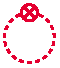
\includegraphics{diagrams/SU2model0d-UFlow_00103_1.pdf}\end{gathered}
	+\input{0d/diagrams/SU2model0d-Uflow_00014_1.tex}\, .\eqTagPrime
\end{align}
This \frg{} flow equation is an exact non-linear \pde{} for the effective potential $U ( t, \sigma )$, which is of first-order in \rgtime{} $t$ and of first- and second-order in the field space direction $\sigma$.
It also includes an explicit $\sigma$-dependence.
A detailed analysis of the structure of this \pde{}, including its relation to the \cfd{} systems, discussed in \cref{sec:conservationLaws}, is provided in \cref{subsubsec:conservative_form}.

For the special case $N = 1$, the $O(N)$ model reduces to the $O(1)$ model.
Such a theory of a single scalar field in zero dimensions, was used in the introductory \cref{sec:0dQFT}.
In this limit, the pion contributions to the flow equation vanish.
As already hinted in \cref{subsubsec:exact_rg_equation}, we find that for non-zero pion contributions ($N > 1$) the flow equation for $U ( t, \sigma )$ acquires a term that is of first-order in the spatial derivative, $\partial_\sigma U ( t, \sigma )$, which no longer has diffusive character, but corresponds to advection in field space.

\subsubsection{FRG Taylor (vertex) expansion}
\label{subsubsec:vertex_expansion}
The \frg{} Taylor expansion is based on the assumption that the effective (average) action $\bar{\Gamma}_t [ \vec{\varphi} \, ]$ can be expanded in a series in field space with \rgtimedependent{} expansion coefficients~\cite{Berges:2000ew}.
Due to the absence of momenta in zero dimensions the \customref{paragraph:taylorExpansion}{FRG Taylor expansion} and the \customref{paragraph:vertexExpansion}{Vertex expansion} of \cref{subsubsec:truncation} are identical and we will use both terms or the combined term \textit{\frg{} Taylor (vertex) expansion} for our discussion.

This expansion in zero dimensions effectively reduces to an expansion of the effective potential $U ( t, \varrho )$, \cf{}\ \cref{eq:ansatz_effective_average_action}.
The \rgscaledependent{} expansion coefficients $\bar{\Gamma}^{(2n)} ( t )$ correspond directly to the scale-dependent vertex functions $\bar{\Gamma}^{(2n)}_{t,\varphi_i \ldots \varphi_i}$ of the \qft{}.
For $d > 0$, these expansion coefficients are usually momentum-dependent in the vertex expansion, whereas in $d = 0$ the coefficients depend only on the \rgtime{} $t$.

The assumption of expandability and thus differentiability significantly restricts the form of the effective action $\bar{\Gamma}_t [ \vec{\varphi} \, ] = U ( t, \vec{\varphi} \, )$, \cf{}\ \ccite{Pangon:2009pj,Pangon:2010uf}.
In fact, it neither allows for the formation of any non-analytic behavior throughout the \frg{} flow nor for any non-analytic \ics{}.
However, non-analytic \ics{} are by no means forbidden, as we will see in \cref{subsec:0dONresults}.
Furthermore, it is well known that non-analyticities can (and in some models have to) form in the effective potential during the \frg{} flow~\cite{Aoki:2017rjl,Grossi:2019urj,Grossi:2021ksl,Borchardt:2016pif} \dash{} especially in the context of dynamic symmetry breaking.
Considering these caveats, an expansion in vertices of a given theory must \apriori{} be approached with caution.
Still, this expansion scheme is widely used in certain applications, \cf{} \veRef{}.

In our work, we restrict our analysis of the precision of this truncation scheme to \frg{} flows with rather specific properties: We study \ics{} that are analytic.
Furthermore, we know, \cf{} \MWApp{}, that the \ir{} effective action is smooth for the special case of zero dimensions, which is a necessary condition for the convergence of a (Taylor) series.
It should, however, be noted that smoothness is only a necessary but not a sufficient condition for the convergence of a Taylor series%
\footnote{%
	A textbook example for a smooth function which has a non-converging Taylor series around $x = 0$ is $$f ( x ) = \begin{cases} \eu^{-1/x} & \text{if } x>0, \\ 0 &\text{else.}\end{cases}$$
}.
Only analyticity would formally imply the convergence of a Taylor series at all $\vec{\varphi}$.
Additionally, we argue that for sufficiently small $N$, the diffusive contributions to the \frg{} flow are important, which smear out any possible cusps.
In summary, we expect that for these extremely special scenarios it is unlikely that non-analyticities will form and disappear again during the \frg{} flow.
Nevertheless, we do not know if a limited number of expansion coefficients is always enough to reach a reliable approximation of $\bar{\Gamma}_t [ \vec{\varphi} \vts ]$ during the \frg{} flow or if it is always necessary to flow the effective potential as a \pde{} without additional assumptions.
This (rather limited) applicability of the \frg{} Taylor expansion to analytic \ics{} will be tested by calculating the relative errors of \ipi{} \nptFunctions{} in the \frg{} Taylor expansion in comparison with the exact results and the results from the flows of a full field-dependent $U ( t, \sigma )$ in \cref{subsec:0dONresults}.\bigskip

The \frg{} Taylor expansion of the zero-dimensional $O(N)$ model is given by the following ansatz~\cite{Keitel:2011pn,Moroz:2011thesis,Pawlowski:talk,Kemler:2013yka},
\begin{align}
	\bar{\Gamma}_t [ \vec{\varphi} \, ] =\, \sum_{n = 0}^{m} \frac{\bar{\Gamma}^{(2n)}(t)}{(2n - 1)!!}\, \frac{1}{n!}\, \bigg( \frac{\vec{\varphi}^{\, 2}}{2} \bigg)^n 
	=\, \bar{\Gamma}^{(0)}(t) + \bar{\Gamma}^{(2)}(t)\,  \frac{\vec{\varphi}^{\, 2}}{2} + \frac{\bar{\Gamma}^{(4)}(t)}{3}\, \frac{1}{2}\, \bigg( \frac{\vec{\varphi}^{\, 2}}{2} \bigg)^2 + \ldots \, ,	\label{eq:vertex_expansion_varphi}
\end{align}
where $\bar{\Gamma}^{(2n)}(t)$ are $t$-dependent expansion coefficients and $m$ is the truncation order.
The factors of $(2n - 1)!!$ and $n!$ were introduced in order to have $\bar{\Gamma}^{(2n)}(t_\mathrm{IR}) = \Gamma^{(2n)}_{\varphi_i \ldots \varphi_i}$ in the \ir{}, where $\Gamma^{(2n)}_{\varphi_i \ldots \varphi_i}$ are the 1PI $2n$-point vertex functions in the \ir{}, with all indices being identical (no summation over $i$ here), see also \cref{eq:on-model_relation_2pf_phi2} \dash{} \eqref{eq:on-model_relation_6pf_phi2}.
In order to arrive at the corresponding flow equations, we proceed in a similar manner as before in \cref{subsubsec:exact_flow_equation_potential}:
We insert our ansatz \eqref{eq:vertex_expansion_varphi} into the full field-dependent two-point function \eqref{eq:full_two-point_function} and use the field space projection operators \eqref{eq:field_space_projection_operators} to invert the latter.
We obtain
\begin{align}
	\big( \bar{\Gamma}^{(2)}_{t,\varphi \varphi} [ \vec{\varphi} \, ] + R_t \big)^{-1}_{i j} =\, \mathcal{P}^\perp_{i j} ( \vec{\varphi} \, ) \, G^{\pi\pi}_t ( \vec{\varphi} \, ) + \mathcal{P}^\parallel_{i j} ( \vec{\varphi} \, ) \, G^{\sigma\sigma}_t ( \vec{\varphi} \, ) \, ,
\end{align}
where
\begin{subequations}
\begin{align}
	G^{\pi \pi}_t ( \vec{\varphi} \, ) \equiv\, & \Bigg[ r ( t ) + \sum_{n = 1}^{m+1} \frac{\bar{\Gamma}^{(2n)}(t)}{(2n - 1)!!}\, \frac{1}{(n - 1)!}\, \bigg( \frac{\vec{\varphi}^{\, 2}}{2} \bigg)^{n-1} \Bigg]^{-1} \, ,
	\\
	G^{\sigma \sigma}_t ( \vec{\varphi} \, ) \equiv\, & \Bigg[ r ( t ) + \sum_{n = 1}^{m+1} \frac{\bar{\Gamma}^{(2n)}(t)}{(2n - 3)!!}\, \frac{1}{(n - 1)!}\, \bigg( \frac{\vec{\varphi}^{\, 2}}{2} \bigg)^{n-1} \Bigg]^{-1} \, ,
\end{align}
\end{subequations}
are the field-dependent propagators of the pion and sigma field in the Taylor expansion.

This result can be inserted into the \frgEquation{}, where the trace in field space is evaluated to
\begin{align}
	\partial_t\, \bar{\Gamma}_t [ \vec{\varphi} \, ] = \, \frac{1}{2} \big[  \partial_t r ( t ) \big] \, \big[  ( N - 1 ) \, G^{\pi \pi}_t ( \vec{\varphi} \, ) + G^{\sigma \sigma}_t ( \vec{\varphi} \, ) \big] \, .\label{eq:wetterich_equation_vertex_expansion}
\end{align}
Finally, we insert the ansatz \eqref{eq:vertex_expansion_varphi} for the \eaa{} into the \lhs{} of this equation and expand the propagators $G^{\circ \circ}_t ( \vec{\varphi} \, )$ up to order $n=m$ in the expansion coefficients $\bar{\Gamma}^{(2n)} ( t )$.
This can also be achieved by successively taking derivatives \wrt{} the fields and setting $\vec{\varphi} = 0$ afterwards.
By comparing the expansion coefficients on the left- and right-hand sides of the equation, one arrives at a coupled set of ordinary differential equations for the $\bar{\Gamma}^{(2n)} ( t )$ with $0 \leq n \leq m$.
The flow equation for $\bar{\Gamma}^{(2m)} ( t )$ contains $\bar{\Gamma}^{(2m+2)} ( t )$ on the right-hand side.
We truncate the system by neglecting the flow of $\bar{\Gamma}^{(2m+2)} ( t )$, \ie{}, assuming $\partial_t \bar{\Gamma}^{( 2 m + 2 )} ( t ) = 0$.

For an automatization of the derivation of the flow equations (the system of \odes{}) via computer algebra routines such as \WAMwR{}, it is advisable to formulate the \frg{} Taylor expansion in the invariant ${\varrho = \tfrac{1}{2} \, \vec{\varphi}^{\, 2}}$,
\begin{align}
	\bar{\Gamma}_t [ \varrho ] =\, & \sum_{n = 0}^{m} \frac{\bar{\Gamma}^{(2n)} (t)}{(2n - 1)!!}\, \frac{\varrho^n}{n!} \, ,
\end{align}
for which \cref{eq:wetterich_equation_vertex_expansion} manifests as
\begin{align}
	\partial_t\, \bar{\Gamma}_t [ \varrho ] =\, & \frac{1}{2} \big[ \partial_t r ( t ) \big] \, \big[ ( N - 1 ) \, G^{\pi\pi}_t ( \varrho ) + G^{\sigma\sigma}_t ( \varrho ) \big] \, ,
\end{align}
while
\begin{subequations}
\begin{align}
	G^{\pi \pi}_t ( \varrho ) \equiv\, & \bigg[ r ( t ) + \sum_{n = 1}^{m+1} \frac{\bar{\Gamma}^{(2 n)} (t)}{( 2 n - 1)!!}\, \frac{\varrho^{n-1}}{(n - 1)!} \bigg]^{-1} \, ,\\
	G^{\sigma \sigma}_t ( \varrho ) \equiv\, & \bigg[ r ( t ) + \sum_{n = 1}^{m+1} \frac{\bar{\Gamma}^{(2 n)} (t)}{( 2 n - 3)!!}\, \frac{\varrho^{n - 1}}{(n - 1)!} \bigg]^{-1} \, .
\end{align}
\end{subequations}
The coupled set of \odes{} for the expansion coefficients $\bar{\Gamma}^{(2n)} ( t )$ is given by~\cite{Keitel:2011pn,Moroz:2011thesis},
\begin{subequations}\label{eq:example_vertex_expansion}
\begin{align}
	\partial_t \bar{\Gamma}^{(0)}( t ) = \, & \frac{N}{2} \,\, \frac{\partial_t r ( t )}{r ( t ) + \bar{\Gamma}^{(2)}( t ) } \, ,	 \label{eq:example_vertex_expansion_zero}	\\
	\partial_t \bar{\Gamma}^{(2)}( t ) = \, & - \frac{N + 2}{6} \, \frac{\partial_t r ( t )}{\big[ r ( t ) + \bar{\Gamma}^{(2)}( t ) \big]^2}  \, \bar{\Gamma}^{(4)}( t ) \, ,	 \label{eq:example_vertex_expansion_two}\\
	\partial_t \bar{\Gamma}^{(4)}( t ) = \, & \frac{N + 8}{3} \, \frac{\partial_t r ( t )}{\big[ r ( t ) + \bar{\Gamma}^{(2)}( t ) \big]^3} \, \big[ \bar{\Gamma}^{(4)}( t ) \big]^2 - \frac{N + 4}{10} \, \frac{\partial_t r ( t )}{\big[ r (t) + \bar{\Gamma}^{(2)}( t ) \big]^2} \, \bar{\Gamma}^{(6)}( t ) \, , \label{eq:example_vertex_expansion_four}\\* % no page break here
	\vdots \mkern7.0mu  &	\nonumber
\end{align}
\end{subequations}
with
\begin{align}
	\forall n \geq 2m+2 \quad \partial_t \bar{\Gamma}^{(n)}(t) = 0 \,
\end{align}
in this approximation.
The system \eqref{eq:example_vertex_expansion} is an explicit example for the tower of equations \nolinebreak[3]\eqref{eq:vertexTower} discussed in \veRef{}.
An alternative derivation to the explicit expansion discussed here can be obtained by using the \textit{higher-order flow equations} of \cref{subsec:higherOrderFlowEquations} for the 
the expansion coefficients $\bar{\Gamma}^{(2n)} ( t )$.

\subsubsection{Conservative form} \label{subsubsec:conservative_form}
\begin{disclaimer}
	This subsubsection follows the discussion presented in Sec.~IV.A of \nbccite{Koenigstein:2021syz}.
\end{disclaimer}
In this subsubsection, we discuss the formulation of the \frg{} flow equation \eqref{eq:flow_equation_effective_potential} as an advection-diffusion equation, as well as its interpretation in the context of \cfd{}, \cf{} \cref{sec:conservationLaws}. 
The fluid-dynamical formulation of the \frg{} flow equation for the effective potential $U ( t, \varrho )$ of models of $O(N)$-type (in the large-$N$ limit~\cite{Tetradis:1995br}) is also presented in recent publications~\cite{Grossi:2019urj,Grossi:2021ksl} by some of our collaborators.
It was shown that the \frg{} flow equation can be recast in the form of a pure advection equation (a hyperbolic conservation law) for the derivative of the effective potential $u ( t, \varrho ) = \partial_\varrho U ( t, \varrho )$, where $u ( t, \varrho )$ serves as the conserved quantity (the fluid), the \rgtime{} $t$ as a temporal coordinate and $\varrho$ as a spatial coordinate.
In this subsubsection, we generalize this result and discuss various consequences for the numerical implementation and interpretation of \frg{} flow equations.
Generalizations of the fluid-dynamical picture of \frg{} flow equations from the large-$N$ results of \ccite{Grossi:2019urj} to systems with finite $N$ as well as the inclusion of fermions were initially presented in various talks, see, \eg{}, \nbccite{WinkHirschegg,Koenigstein:2020Talk}.
Further early developments in this context are discussed in the master thesis~\cite{Ihssen2020} of Friederike Ihssen, the PhD thesis~\cite{Wink:2020tnu} of Nicolas Wink, and also in \ccite{Grossi:2021ksl}.
Furthermore, \ccite{Aoki:2017rjl} includes a formulation of the flow equation as a conservation law and a discussion of shock waves based on the characteristics is presented, however, without really elaborating on a fluid-dynamical interpretation and its consequences.\bigskip

The formulation of \frg{} flow equations in terms of a fluid-dynamical language has two  major advantages:
\begin{enumerate}
	\item It provides an intuitive explanation for different kinds of phenomena observed in \frg{} flow equations, \eg{}, the flattening of the effective potential for small $\sigma$ in the \ir{}, which occurs in conjunction with a non-differentiable point of the effective potential at the ground state.
	Such non-analytic behavior cannot be handled and systematically analyzed by commonly used numerical schemes such as the Taylor expansion or related discretization schemes for the effective potential, since the latter strongly rely on differentiability.
	However, these phenomena have a direct impact on the physics, for instance on the occurrence of phase transitions~\cite{Aoki:2017rjl,Bonanno:2004pq,Pangon:2009pj,Pangon:2010uf,Grossi:2019urj,Wipf:2013vp,Ehrenfest1933,Grossi:2021ksl}, and therefore must be resolved and analyzed accurately also on a numerical level.
	
	\item The formulation of the \frg{} flow equations in terms of fluid-dynamical concepts provides access to the highly developed and extremely powerful toolbox of \cfd{}, \cf{} \cref{sec:conservationLaws}, which finds applications in a wide area of fields, ranging from the natural sciences and engineering all the way to economics.
	Recasting \frg{} flow equations as conservation laws allows a direct application of the numerical methods, \viz{} the \ktScheme{}, and the related \cfd{} concepts established in \cref{sec:conservationLaws}.
\end{enumerate}	
Interestingly, the idea of interpreting \rg{} flow equations as ``flow'' equations in the true sense of the word is not new and explains the term ``\textit{RG flow equations}'': A discussion of analogies between ``RG flow'' and hydro-dynamical flow can be found in widely used textbooks~\cite{Peskin:1995ev,Coleman:1985rnk} and is discussed via the example of field-independent coupling constants in the context of perturbative renormalization.
Furthermore, the \rg{} flow was already associated with gradient flow and dissipative processes in \ccite{Wallace:1974dx,Wallace:1974dy,Zamolodchikov:1986gt,Zumbach:1994vg,Zumbach:1994kc,Zumbach:1994vg,Rosten:2010vm}, even though a stringent fluid-dynamical interpretation and formulation was not presented. 

It is therefore also not accidental that the \grg{} community has chosen the term ``\rgtime{}'' for the logarithm of the \rgscale{} $k$ over the \uv{} scale $\Lambda$, $\tilde{t} = \ln \big( \tfrac{k}{\Lambda} \big)$. 
In contrast, we find that $t = - \tilde{t} \in [ 0, \, \infty )$ can be naturally identified as a temporal coordinate in the fluid-dynamical picture of \grg{} flow equations, see below.
Hence we outright adopted the latter convention for this thesis, \cf{} \cref{eq:def_rg_time}.
An interpretation of the scale-dependent generation functionals $\mathcal{Z}_t [ J ]$ or $\mathcal{W}_t [ J ]$ as functional flow equations in \cref{subsec:RGflow} was part of our methodological introduction in \cref{chap:methods}.
We now want to discuss this explicitly in zero dimensions unburdened by the functional nature of the general expressions.

Considering the obvious analogies between flow equations arising in the \frg{} framework and fluid-dynamical equations, it is remarkable that the \frgEq{} has not been more systematically investigated and compared to well-known fluid-dynamic equations.
For the related \rg{} flow equations the situation is slightly different and the mathematical analysis on the level of \pdes{} was more systematic, see, \eg{}, \ccite{Felder:1987,Hasenfratz:1985dm,Zumbach:1994kc,Zumbach:1994vg,Rosten:2010vm}.
Furthermore, certain phenomena well-known in fluid dynamics, such as discontinuities (shock waves), rarefaction waves, or cusps, occur in the solution of such \pdes{}.
These require a careful numerical treatment to resolve them, but their occurrence was very often ignored by numerical approaches to solve the Wetterich equation by erroneously assuming that the solution $U ( t, \sigma )$ is continuous, smooth, and differentiable.
Still, there are some publications which use numerical schemes to systematically capture non-analytic behavior or discuss the limitations of numerical methods in the presence of these effects, see, \eg{}, \ccite{Borchardt:2016pif,Aoki:2017rjl}.

In order to make the fluid-dynamical analogy apparent, we present a formulation of the \frg{} flow equation \eqref{eq:flow_equation_effective_potential} for the effective potential $U ( t, \sigma )$ in terms of a conservation law.
Furthermore, we discuss its fluid-dynamical interpretation on a qualitative level and classify the various contributions to the \pde{} \dash{} the \grg{} flow \dash{} in the fluid-dynamical picture.
This sets the stage for an adequate qualitative interpretation of the \frg{} flow equation and a direct application of the \ktScheme{} established in \cref{subsec:hydroKT}.\bigskip

{%
\hypersetup{linkcolor=black}%
\paragraph{The conservative form of Eq. \textbf{(\protect\ref{eq:flow_equation_effective_potential})}}\phantomsection\label{paragraph:conservative_form_equation}\mbox{}%
}\\
Starting from the \frg{} flow equation \eqref{eq:flow_equation_effective_potential} of the effective potential $U ( t, \sigma )$, we have several options to recast the flow equation in a conservative form, two of which are:
\begin{enumerate}
	\item	Following \ccite{Aoki:2017rjl,Grossi:2019urj,Grossi:2021ksl,WinkHirschegg,Wink:2020tnu,Ihssen2020}, we can take an overall derivative of \cref{eq:flow_equation_effective_potential} \wrt{} the $O(N)$ invariant $\varrho = \tfrac{1}{2}\,\sigma^2$ and express the resulting equation in terms of $\varrho$ and $u ( t, \varrho ) \equiv \partial_\varrho U ( t, \varrho )$,
		\begin{align}
			\partial_t u ( t, \varrho ) = \dod{}{\varrho}\! \bigg( \frac{1}{2} \, \frac{N - 1}{r ( t ) + u ( t, \varrho )}\,\partial_t r ( t )  + \frac{1}{2} \, \frac{1}{r ( t ) + u ( t, \varrho ) + 2 \varrho \, \partial_\varrho u ( t, \varrho )}\,\partial_t r ( t )  \bigg) \, .	\label{eq:conservation_law_u_rho}
		\end{align}

	\item	Another option is to formulate the problem on the level of the background field $\sigma$ itself~\cite{Koenigstein:2020Talk} and by alternatively defining $u ( t, \sigma ) \equiv \partial_\sigma U ( t, \sigma )$. 
	Taking an overall derivative of \cref{eq:flow_equation_effective_potential} \wrt{} $\sigma$ yields,
		\begin{align}
			\partial_t u ( t, \sigma ) = \dod{}{\sigma} \! \bigg( \frac{1}{2} \, \frac{N - 1}{r ( t ) + \frac{1}{\sigma} \, u ( t, \sigma )}\,\partial_t r ( t )  + \frac{1}{2} \, \frac{1}{r ( t ) + \partial_\sigma u ( t, \sigma )}\,\partial_t r ( t )  \bigg) \, .	\label{eq:conservation_law_u_phi}
		\end{align}
\end{enumerate}
In both cases one ends up with a one-dimensional conservation law, where $u$ plays the role of the conserved quantity (the fluid), $t$ can be identified with the time variable and $\varrho$ or $\sigma$ are identified as the spatial variable.

The conservative form of the \frg{} flow equation \eqref{eq:flow_equation_effective_potential} for the effective potential $U$ on the level of its derivative $u$ is not restricted to zero space-time dimensions or models with purely bosonic field content, see also \ccite{Aoki:2017rjl,Grossi:2019urj,Grossi:2021ksl,WinkHirschegg,Koenigstein:2020Talk,Wink:2020tnu,Ihssen2020} and \cref{chap:GN,chap:QMM}.
As a matter of fact, this formulation generalizes to arbitrary dimensions and also to models which include fermionic degrees of freedom on the level of the \lpa{}.
In particular, the flow equation for the effective potential for models of strong-interaction matter, such as the quark-meson, the Nambu-Jona-Lasinio, and the Gross-Neveu(-Yukawa) model can be formulated in this fashion~\cite{Ihssen2020,Grossi:2021ksl,Stoll:2021ori,Ihssen:2022xkr,Ihssen:2023xlp}.

In this context, it is also worthwhile to note that \cref{eq:conservation_law_u_phi} can be derived not only by taking a derivative of the \frg{} flow equation for the effective potential $U ( t, \sigma )$ \wrt{} the background field $\sigma$.
It is also possible to use the flow equation for the one-point function \eqref{eq:FS1} directly and hence deriving the flow equation for $u ( t, \sigma )$ via a projection on the one-point function $\bar{\Gamma}_t^{(1)} ( \sigma \, )$,
	\begin{align}
		\partial_t u ( t, \sigma ) &= \, \big( \partial_t \bar{\Gamma}_t^{,\sigma} [ \vec{\varphi} \, ] \big)_{\varphi_1 = \ldots = \varphi_{N - 1} = 0 , \, \varphi_{N} = \sigma}\equiv\partial_t \FSvertexArg{\FSeaaEoM}{\sigma}\label{eq:0dON1pt}\\[.2em]
		&=\,
		-\frac{1}{2}\,\begin{gathered}\raisebox{-6pt}{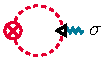
\includegraphics{0d/diagrams/SU2model0d-dUFlow_00203_1.pdf}}\end{gathered}
		-\frac{1}{2}\,\begin{gathered}\raisebox{-6pt}{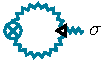
\includegraphics{0d/diagrams/SU2model0d-dUFlow_00024_1.pdf}}\end{gathered}\\
		&=\, - \frac{1}{2} \, \frac{N - 1}{\big[ r ( t ) + \frac{1}{\sigma} \, u ( t, \sigma ) \big]^2} \, \partial_\sigma \big[ \tfrac{1}{\sigma} \, u ( t, \sigma ) \big]\,\partial_t r ( t ) -\nonumber\\
		&\qquad\qquad\qquad\qquad\qquad\qquad- \frac{1}{2} \,  \frac{1}{\big[ r ( t ) +  \partial_\sigma u ( t, \sigma ) \big]^2} \, \partial_\sigma^2 u ( t, \sigma )\,\partial_t r ( t ) \\
		&=\, \dod{}{\sigma}\! \Bigg(
		\frac{1}{2}\,\begin{gathered}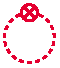
\includegraphics{diagrams/SU2model0d-UFlow_00103_1.pdf}\end{gathered}
		+\input{0d/diagrams/SU2model0d-Uflow_00014_1.tex}
		\Bigg) \, .
	\end{align}
This corresponds to an interchange in the order of operations (evaluating the Wetterich equation on the background field configuration and taking derivatives \wrt{} the background field versus taking functional derivatives of the \frg{} equation and afterwards evaluating on the background field) and it is non-trivial (especially for flow equations for more complex models in higher dimensions and with truncation beyond \lpa{}) that the resulting equations are identical, \cf{} \cref{app:SU2}.

Before we turn to the fluid-dynamical interpretation of the conservation laws~\eqref{eq:conservation_law_u_rho} and \eqref{eq:conservation_law_u_phi}, we comment on the question whether one of the two formulations~\eqref{eq:conservation_law_u_rho} and \eqref{eq:conservation_law_u_phi} is preferable or if even others should be considered.
The answer to this question is not yet settled. 
From our present understanding, a formulation of the conservation equation in terms of $\sigma$ is preferable, for reasons of numerical implementability in the \fv{} scheme we use.
This is discussed at length in the context of the \pde{} \bcs{} for the \frg{} flow equation in \cref{subsec:boundary_conditions_finite_volume}.
Therefore, our discussion in the next sections is based on \cref{eq:conservation_law_u_phi}, and hence we identify $\sigma$ with the spatial coordinate $x$ and $u ( t, \sigma ) \equiv \partial_\sigma U ( t, \sigma )$ as the conserved quantity.\bigskip

The rest of this subsubsection is dedicated to the fluid-dynamical interpretation of the \frg{} flow equation \eqref{eq:conservation_law_u_phi}.
To this end, we split the flux (current) on the \rhs{} of the conservation law \eqref{eq:conservation_law_u_phi} and rewrite the whole equation in terms of an advection-diffusion equation, \cf{} \cref{eq:FVadsEq} and \cref{subsec:hydroAdvection,subsec:hydroDiffusion}, in one spatial dimension $x = \sigma$ and one temporal dimension $t$,
\begin{align}
	\partial_t u ( t, x ) + \dod{}{x} F [ t, x, u ( t, x ) ] = \dod{}{x} Q [ t, \partial_x u ( t, x ) ] \, .	\label{eq:advection_diffusion_equation_zero-dimensional}
\end{align}
The pionic contributions to the \frg{} flow,
\begin{align}
	F [ t, x, u ( t, x ) ] = \, & - \frac{1}{2} \, \frac{N - 1}{r ( t ) + \frac{1}{x} \, u ( t, x )}\, \partial_t r ( t ) = -\frac{1}{2}\,\begin{gathered}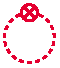
\includegraphics{diagrams/SU2model0d-UFlow_00103_1.pdf}\end{gathered} \, ,\label{eq:advection_flux_pion_propagator}
\end{align}
are identified with a non-linear, position-dependent advection flux, while the contribution of the radial \sigmaMode{},
\begin{align}
	Q [ t, \partial_x u ( t, x ) ] = \, & + \frac{1}{2} \,  \frac{1}{r ( t ) + \partial_x u ( t, x )}\, \partial_t r ( t ) = \input{0d/diagrams/SU2model0d-Uflow_00014_1.tex}\, ,\label{eq:diffusion_flux_sigma_propagator}
\end{align}
corresponds to a non-linear diffusion flux.
We discussed conservation equations like \cref{eq:advection_diffusion_equation_zero-dimensional} in a \cfd{} context at length in our methodological introduction~\ref{sec:conservationLaws}.
In the following paragraphs we want to comment on the nature of the pionic/advective and radial $\sigma$/diffusive contributions using the established \cfd{} terminology.

\paragraph{Advection}\phantomsection\label{paragraph:conservative_form_advection}\mbox{}\\
If we ignore the contribution of the \sigmaMode{} for a moment (which \dash{} after rescaling \dash{} corresponds to the large-$N$ limit of the $O(N)$ model~\cite{Grossi:2019urj,Tetradis:1995br,Grossi:2021ksl,Steil:2021cbu}), we can rewrite the \lhs{} of \cref{eq:advection_diffusion_equation_zero-dimensional} as follows,
\begin{align}
	\partial_t u ( t, x )& + \dod{}{x} F [ t, x, u ( t, x ) ] =  0 \label{eq:advection_zero-dimensional} \\[.2em]
	\partial_t u ( t, x )& + \partial_u F [ t, x, u ( t, x ) ] \, \partial_x u ( t, x ) +\partial_x F [ t, x, u ( t, x ) ] = 0 \label{eq:advection_zero-dimensional_primitive}
\end{align}
This is a hyperbolic, non-linear advection equation for $u ( t, x )$, \cf{} \cref{eq:FVadsEqFonly}, and its accompanying \textit{primitive form}, \cf{} \cref{eq:FVFprimitive}, including an internal source term.
$\partial_u F [ t, x, u ( t, x ) ]$ is identified with the velocity of the characteristics (the local $u$-dependent flow velocity of the quantity $u$) and $\partial_x F [ t, x, u ( t, x ) ]$ acts like an $x$- and $u$-dependent internal source term.  
Hence $F [ t, x, u ( t, x ) ]$ is not purely advective nevertheless we will continue to refer to it as advection term.

The form of \cref{eq:advection_zero-dimensional} motivated our discussion of linear and non-linear advection equations in \cref{sububsec:LAEBBE} with the \laeq{} and \bbeq{} as instructive examples.
When compared to the \bbeq{} we notice that in our pionic \frg{} flow the local flow velocity is highly non-linear in $t$, $x$ and $u$ and explicitly reads
\begin{align}
	\partial_u F [ t, x, u ( t, x ) ] = \, & \frac{1}{2}\,\frac{ N - 1 }{x \, \big[ r ( t ) + \frac{1}{x} \, u ( t, x ) \big]^2}\,\partial_t r ( t ) \, .	\label{eq:advection_velocity}
\end{align}
Considering for example the exponential regulator shape function \eqref{eq:exponential_regulator}, one finds that the advection velocity $\partial_u F [ t, x, u ( t, x ) ]$ is always negative (positive) for $x > 0$ ($x < 0$).
In a fluid-dynamical picture, this means that the conserved quantity $u ( t, x )$ is always propagated from larger values of $|x|$ towards the point $x = 0$ by advection.
Furthermore, the closer the fluid $u ( t, x )$ is to $x = 0$, the faster the fluid moves, due to the factor $\frac{1}{x}$.
Since $u ( t, x )$ is antisymmetric in $x$, because of the $O(N)$ symmetry of $U ( t, \vec{\varphi} \, )$, this implies that ``waves'' of positive and negative $u ( t, x )$ collide with huge velocity at $x = 0$ and annihilate.
At large $|x|$, the fluid velocity tends to zero.

We also observe that the advection velocity \eqref{eq:advection_velocity} is proportional to the number of pions, $ N - 1 $.
Hence, in the large-$N$ limit the system, discussed at length in \cref{subsec:0dLargeN}, is completely advection driven, while for small $N$ the diffusive contributions \eqref{eq:diffusion_flux_sigma_propagator} gain in importance.
In the case $N = 1$, discussed at length in \cref{subsec:0dO1Entropy}, there is no advection at all and the dynamics of the fluid $u ( t, x )$ is purely diffusive.

At this point we want to remind the reader of the general properties and features of non-linear advection equations \dash{} like shock formation, (numerical) entropy production, and irreversibility \dash{}
discussed in general in \cref{subsec:hydroAdvection}.
Naturally those properties also play an important role in the dynamics of \frg{} flows, which we will discuss in the following conceptually and also using explicit examples.

\paragraph{Diffusion}\phantomsection\label{paragraph:conservative_form_diffusion}\mbox{}\\
Next, we turn to the contribution of the radial \sigmaMode{} to the \frg{} flow. 
We find that it enters the conservation law \eqref{eq:advection_diffusion_equation_zero-dimensional} as a non-linear diffusion flux \eqref{eq:diffusion_flux_sigma_propagator}, because it is overall of second-order in spatial derivatives of $u ( t, x )$. 
The characteristic property of diffusive processes is that they transport a quantity, in this case $u ( t, x )$, from regions where its density or concentration is high to regions where it is low~\cite{LeVeque:1992,LeVeque:2002,RezzollaZanotti:2013,Ames:1992}, \cf{} \cref{subsec:hydroDiffusion}.
Diffusive processes are therefore usually important in regions of high gradients and smear out cusps, shocks \etc{}, which might form via advection.
Besides this, diffusive processes are generically undirected, which is also the case for the diffusion flux \eqref{eq:diffusion_flux_sigma_propagator} which propagates the quantity $u ( t, x )$ in both directions, depending on the local gradients of $u ( t, x )$, which is especially relevant for models in their symmetry-broken phase with rather weak advection (small $N$). 
The effective transport velocities via diffusion are usually much slower than those via advection, which is, due to the non-linearity, not necessarily true for \frg{} flow equations.
We discussed the \heq{} as an archetypal linear diffusion equation at length in \cref{paragraph:HE}.
The diffusion flux \eqref{eq:advection_diffusion_equation_zero-dimensional} can be formulated as a non-linear time-dependent realization of the heat equation.
By performing the spatial derivative in the advection-diffusion equation \eqref{eq:advection_diffusion_equation_zero-dimensional} for the purely diffusive ($N = 1$) case, one finds
\begin{align}
	\partial_t u ( t, x ) = \, & \alpha[t,\partial_x u ( t, x )] \, \partial_x^2 u ( t, x ) \, ,\label{eq:0ddifprim}
\end{align}
where
\begin{align}
	\alpha[t,\partial_x u ( t, x )] \equiv - \frac{\tfrac{1}{2} \, \partial_t r ( t )}{[ r ( t ) + \partial_x u ( t, x ) ]^2} \, ,	\label{eq:diffusion_coefficient}
\end{align}
plays the role of a non-linear time-dependent, strictly positive \dash{} parabolic \dash{} diffusion coefficient. 
The positivity of the diffusion coefficients ensures that $u ( t, x )$ is only dispersed and never accumulates locally, \ie{}, that $u ( t, x )$ tends to equilibrate towards a linear function in space. 
A positive diffusion coefficient also ensures stability and uniqueness of (numerical) weak solutions, as discussed in the beginning of \cref{subsec:hydroDiffusion}.

Directly comparing these findings with the \he{}, we can already qualitatively predict the behavior of the diffusion transport for the \frg{} flow of $u ( t, x )$, as long as $N$ is small and the system is diffusion-dominated.
At a constant \rgtime{} $t$, we find that the diffusion coefficient is much larger in regions where the gradient $\partial_x u ( t, x )$ is negative with a large absolute value, compared to regions where it is positive, because in the first case the denominator of \cref{eq:diffusion_coefficient} is smaller than in the second case.
This plays a crucial role for systems that involve symmetry breaking, where $\partial_x u ( t, x )$ is negative for at least some small $|x|$, while asymptotically for $|x| \rightarrow \infty$ the sign of $\partial_x u ( t, x )$ is always positive.
Hence, for diffusion-dominated problems in \frg{} flow equations (small number $N$ of pions), the symmetry restoration is driven by the negative gradients $\partial_x u ( t, x )$ at small $|x|$.
Furthermore, we find that for $t \rightarrow \infty$, the numerator of the diffusion coefficient \eqref{eq:diffusion_coefficient} tends to zero such that the diffusion stops, the system equilibrates and the dynamics freezes, even though there are still gradients in $u ( t, x )$.
This would not happen for the linear \he{} with its constant diffusion coefficient.
The same is true for $t = 0$, where the diffusion coefficient is suppressed by $1/\Lambda$.

\paragraph{Irreversibility and entropy production}\phantomsection\label{paragraph:conservative_form_entropy}\mbox{}\\
In a fluid-dynamical setting, it is very easy to understand the role of the radial \sigmaMode{}: Due to its diffusive character, it is directly responsible for the irreversibility of the \grg{} flow and \rg{} transformations in general. 
Diffusion is a particular example of a dissipative process, which is irreversible and increases the entropy of the system\footnote{%
	Interestingly, \ccite{Zamolodchikov:1986gt} comes to the same conclusion arguing in reverse order:
	``Some of the information on the ultraviolet behavior of the field theory is lost under renormalization transformations with $t>0$, since in the field theory it is not legitimate to examine correlations at scales smaller than the cutoff.
	We would therefore expect that a motion of the space $Q$ [a change of the set of all couplings] under the influence of the renormalization group would become an `irreversible' process, similar to the time evolution of dissipative systems.''
	We remark that also \ccite{Zumbach:1994vg} stated that a term of second-order in field space derivatives in related \rg{} flow equations ``[\ldots] corresponds to a dissipation in the flow and is responsible for the semi-group property of the \rg{}''.%
}.
The dissipative and irreversible character can be seen as a ``thermodynamic'' version of the irreversible Kadanoff block-spin transformations~\cite{Kadanoff:1966wm,Wilson:1979qg,Delamotte:2007pf}.
Hence, the dissipation clearly singles out the \rgtime{} $t$ as a temporal direction, because it introduces a ``thermodynamic arrow of time'' and ``thermodynamic time asymmetry'' via entropy production~\cite{Lebowitz:2008}.
This also explains why our definition \eqref{eq:def_rg_time}:
\begin{align}
	&t \equiv - \ln \big( \tfrac{k}{\Lambda} \big) =  \ln \big( \tfrac{\Lambda}{k} \big) \, ,	\qquad	t \in [ 0, \infty ) \, .	\label{eq:rg-time-scale}
\end{align}
is a natural choice for a temporal coordinate also in higher dimensions, see also \ccite{Hasenfratz:1985dm,Zumbach:1993zz,Zumbach:1994vg,Zumbach:1994kc,Grossi:2019urj}.

Interestingly, the irreversibility and the dissipative character of the system is lost if one does not include the full field-dependence of the effective potential in the flow equation, but instead uses a truncated system like the Taylor expansion \eqref{eq:example_vertex_expansion}.
Then, the system \eqref{eq:example_vertex_expansion} of coupled \odes{} for the vertices can theoretically be integrated in either direction in \rgtime{}, as long as it consists of a finite number of couplings\footnote{%
	In momentum space this enables an integration to higher energy scales, which corresponds to a reversion of the coarse-graining in position space.
	More generally speaking, this implies that it is possible to resolve the microphysics from the macrophysics.
	Both are physically not possible and solely an artifact of the truncation.%
}.
The most extreme examples are the \rg{} flows of one single $t$-dependent coupling, \eg{}, the quartic coupling of $\phi^4$ theory or the \qcd{} beta function~\cite{Politzer:1973fx,Gross:1973id,Gross:1973ju,Gross:1974cs}, see also the textbooks~\cite{ZinnJustin:2002ru,Peskin:1995ev}.
Here the integration to both higher and smaller \rgscales{} is possible, which is the well-known result for the universal one-loop beta function and is an artifact of the restriction (truncation) to a finite number of couplings~\cite{Wilson:1979qg}.
However, this reversibility of \rg{} transformations is not possible for the field-dependent effective potential, which is obvious from the advection-diffusion equation~\eqref{eq:advection_diffusion_equation_zero-dimensional}, where entropy increases and the information about the \ic{} in the \uv{} cannot be recovered from the \ir{} anymore.

This point of view was already shared, presented, and discussed by K.~G.~Wilson:
In \nbccite{Wilson:1979qg} he pointed out the differences between his ``coarse-graining'' version of the \rg{}, which is also applicable in highly non-perturbative regimes, and the \rg{} flow equations used by C.~Callan, K.~Symanzik, M.~Gell-Mann, F.~Low, G.~t'Hooft, S.~Weinberg, H.~Georgi, D.~Politzer and others to calculate the running of a single (or small number of) coupling constants, which solely describes a system correctly in a perturbative regime.

The irreversibility of the \frg{} flow and entropy production is also directly related to the presence of discontinuities in the solution, which can arise from the advective contributions to the flow.
As shown in \ccite{Aoki:2017rjl,Grossi:2019urj,Grossi:2021ksl,Steil:2021cbu} for the large-$N$ limit, a shock wave arises when the weak solution of the \pde{} is multi-valued. 
The correct solution is usually constructed by means of the Rankine-Hugoniot condition~\cite{Rankine:1870,Hugoniot:1887,LeVeque:1992,LeVeque:2002,RezzollaZanotti:2013,Ames:1992}.
This would lead to ambiguities when one tries to invert the flow (integrating backwards in time) in the presence of a shock.
Hence, shock formation is an irreversible process and produces entropy.
In summary, these are further strong arguments why the assumption of expandability of the effective average action in terms of vertices as well as the truncation of the system should in general be considered with care.

Therefore, it would be extremely interesting to explicitly construct an entropy function for the flow equation, \ie{}, a quantity that is either non-decreasing or non-increasing under the \rg{} transformations during the \frg{} flow (depending on the sign convention), and that is a functional of the quantity $u ( t, x )$.
The entropy for the flow equation will be a helpful instrument to design a stable numerical scheme for generic truncations~\cite{LeVeque:1992,LeVeque:2002,RezzollaZanotti:2013} and will also highlight general properties of the \grg{} flow.
In this context we also have to mention the recent publication~\cite{Cotler:2022fze} by J. Cotler and S. Rezchikov who were able to interpret the Polchinski equation as an ``optimal transport gradient flow of a field-theoretic relative entropy'' thus establishing a firm and explicit connection between an information-theoretic entropy and (F)RG flows.

Additionally, a numeric entropy (function) might provide a direct link to $\mathcal{C}$-/$\mathcal{A}$-theorems~\cite{Zamolodchikov:1986gt,Banks:1987qs,Cardy:1988cwa,Osborn:1989td,Jack:1990eb,Komargodski:2011vj,Curtright:2011qg,Rosten:2010vm}, which state that in certain \qfts{} there exists some positive real function $\mathcal{C} ( \{ g_i \} , t )$, which depends on all coupling constants of the QFT and which is monotonically increasing\footnote{%
	It can also be defined as a monotonically decreasing function.
	This flip of sign corresponds to the difference of the mathematicians' and physicists' definition of entropy.
	We chose to the ``thermodynamic convention'' of increasing entropy for this and subsequent publications.
} during \rg{} flows (transformations), while it stays constant at (critical) fixed points,
	\begin{align}
		\dod{}{t} \mathcal{C} ( \{ g_i \} , t ) \geq 0 \, .
	\end{align}
Here, $\{ g_i \}$ denotes the set of all (possibly infinitely many) dimensionless coupling constants.
In contrast to previous formulations~\cite{Haagensen:1993by,Generowicz:1997he,Forte:1998dx,Codello:2013iqa,Codello:2015ana,Becker:2014pea,Becker:2016zcn}, a non-local version, which is directly linked to the numerical entropy function (similar to versions presented in \ccite{Zumbach:1993zz,Zumbach:1994vg,Rosten:2010vm} for related field-dependent flow equations), would not rely on expandability in the couplings or vertices and could naturally display the dissipative character of \rg{} transformations, which was already described by \ccite{Zamolodchikov:1986gt,Zumbach:1994vg}.
Fixed-point solutions of the \frg{} flow would directly correspond to steady-state or thermal-equilibrium solutions~\cite{LeVeque:1992} in the fluid-dynamical picture\footnote{%
	This actually brings up the interesting question whether previous studies about global fixed-point solutions for field-dependent flow equations, which seemed to deliver interesting results, \eg{}, \ccite{Borchardt:2015rxa,Zumbach:1994vg,Yabunaka:2018mju}, should be reanalyzed from the fluid-dynamical steady-flow perspective, especially regarding their interpretation and the spatial discretization methods~\cite{LeVeque:1992}.
}.
A caveat at this point is that a $\mathcal{C}$ function is based on the rescaled dimensionless \rg{} flow equations.
Hence, also a numerical entropy should be formulated in this framework, if one seeks a direct link to a $\mathcal{C}$ function.
The dimensionless flow equations in the \lpa{} can be recast in terms of conservation laws, which might be a good starting point.

An explicit discussion of (numerical) entropy for the zero-dimensional $O(1)$ model as well as possible links to $\mathcal{C}$ functions is discussed in great detail in \cref{subsec:0dO1Entropy}.
The situation for the $O(N)$ model in the limit $N\rightarrow\infty$ is discussed in \cref{subsec:0dLargeN}.
The construction of an explicit (numerical) entropy has proven to be elusive in the case of finite $N>1$ for the $O(N)$ model~\cite{Koenigstein:2021rxj,Steil:2021cbu} due to the explicit position-dependencies in \cref{eq:conservation_law_u_phi} and \eqref{eq:conservation_law_u_rho} and the related internal source terms, \cf{} \cref{eq:advection_zero-dimensional}.

\paragraph{Generalizations}\phantomsection\label{paragraph:conservative_form_generalizations}\mbox{}\\
At this point we want to briefly comment on the generalization of the fluid-dynamical picture to \frg{} flow equations in higher-dimensional \qfts{}, systems with more (field-dependent) couplings, and \frg{} flow equations that involve fermions.

In higher-dimensional \qfts{}, the fluid-dynamical interpretation of the \frg{} flow of the effective potential survives, see for example \ccite{Grossi:2019urj,Grossi:2021ksl,Koenigstein:2020Talk,Stoll:2021ori,Ihssen:2022xkr,Ihssen:2023xlp} and especially \cref{chap:GN}.
In zero dimensions, $t$ merely parametrizes some dimensionless (mass-like) scale $r ( t )$, see \cref{eq:exponential_regulator}. 
In contrast, in higher dimensions, the \rgtime{} is defined as the negative logarithm of the ratio between the \rg{} momentum scale $k$ and the \uv{} reference scale $\Lambda$, see \cref{eq:rg-time-scale}.
The fluxes gain further $t$-dependent prefactors via the momentum integrals of the trace in the Wetterich equation.
This leads to a different time scaling but does not affect the overall discussion. 
The inclusion of further field-independent but scale-dependent couplings (such as a scale-dependent Yukawa coupling) adds \odes{} to the advection-diffusion equation for the effective potential, which does not spoil its conservative fluid-dynamical character.
It is currently investigated by us and collaborators~\cite{Ihssen2020,Grossi:2021ksl,Ihssen:2022xkr,Ihssen:2023nqd,Ihssen:2023xlp} whether the inclusion as well as the conservative formulation of further field-dependent couplings (such as a field- and scale-dependent wave-function renormalization $Z ( t, \vec{\varphi} \, )$ in higher-dimensional models) is possible.
In any case, simply adding fermions in the \lpa{} does not destroy the fluid-dynamical character of the \frg{} flow equation at all: On the level of the \lpa{} for the \frg{} flow equation of the effective potential, the contributions from fermion loops can be interpreted as a source/sink term, which only depends on $\sigma$, \ie{}, the spatial position $x$.
We discuss such fermionic source/sink terms in zero dimensions in \cref{sec:0dSU2} and in non-zero, \ie{}, $1\dimSpacer + \dimSpacer 1=2$ dimensions, at zero and non-zero temperature and especially quark chemical potential in \cref{chap:GN}.
Another possible generalization concerns models with more than one invariant of the underlying symmetry group of the model and respective condensation directions in field space, see, \eg{}, \ccite{Strodthoff:2011tz,Mitter:2013fxa,Rennecke:2016tkm,Lakaschus:2020caq,Fukushima:2010ji,Fejos:2020lli}.
Here, the fluid-dynamical framework should still be applicable.
However, a suitable identification of a complete basis of field space directions with ``spatial directions'' of the fluid-dynamical problem and a clear separation of the single contributions into advection, diffusion, and source terms might be challenging and calls for future investigations \dash{} especially when it comes to an actual numerical implementation.
For first attempts of generalizing our findings to a quark-meson-diquark model, we refer to \ccite{Lakaschus:2021ewd}.

Summarizing we find that the fluid-dynamical interpretation of flow equations has tremendous benefits, because it allows for a rather intuitive understanding of the dynamics of the system. Furthermore, it allows for a novel, physically intuitive interpretation of the \frg{} flow and provides an understanding of its irreversibility.
Finally, it opens up the opportunity to employ extremely powerful numerical tools from \cfd{}.

\subsubsection{Boundary conditions and computational domain}\label{subsec:boundary_conditions_finite_volume}
\begin{disclaimer}
	This subsubsection follows the discussion presented in Sec.~IV.D of \nbccite{Koenigstein:2021syz}.
\end{disclaimer}
In the form of the conservation laws \eqref{eq:conservation_law_u_rho} or \eqref{eq:conservation_law_u_phi}, the \frg{} flow equation \eqref{eq:flow_equation_effective_potential} is a non-linear \pde{} which has contributions of parabolic (diffusion terms) as well as hyperbolic (advection terms) nature.
In this subsubsection, we specify the \bcs{} for Eqs.~\eqref{eq:conservation_law_u_rho} or~\eqref{eq:conservation_law_u_phi} in field space (the effective spatial $x$-direction).

For (non-linear) \pdes{} of hyperbolic and parabolic type, the spatial \bcs{} are needed (in addition to the \ic{}) to make finding a (weak) solution a well-defined problem, \cf{} \cref{subsec:hydroAdvection,subsec:hydroDiffusion}.
We are dealing with a \textit{Cauchy} or to be even more specific an \textit{initial-boundary-value} problem.
Thus, without explicitly specifying the \bcs{}, \eg{}, of Neumann- or Dirichlet-type, as well as the \ics{}, the problem of finding a unique (weak) solution is actually ill-posed and therefore impossible to solve \dash{} a well-known mathematical fact with particular and severe implications in, \eg{}, classical electrodynamics~\cite{Jackson:1998nia}, fluid dynamics~\cite{BuckleyLeverett:1942}, soliton and instanton solutions of classical field equations~\cite{Rajaraman:1982is,Shifman:1994ee}, general relativity~\cite{Weinberg:1972kfs,Misner:1974qy,Ryder:2009zz}, and other fields of research.
This \dash{} unsurprisingly \dash{} also holds true for the \frg{}. 
However, explicit \bcs{} and especially their numerical implementation are rarely discussed in \frg{} literature, with, \eg{}, \ccite{Caillol:2012zz,Pangon:2009pj,Pangon:2010uf,Codello:2013iqa} as notable exceptions before the advent of \cfd{} methods for the \frg{}~\cite{Grossi:2019urj,zerod1,zerod2,zerod3,Ihssen2020,Stoll:2021ori,Grossi:2021ksl,Ihssen:2022xkr,Ihssen:2023nqd,Ihssen:2023xlp}.

For the derivative of the effective potential $u ( t, \sigma )$, we find that the spatial \bcs{} must be imposed at $\sigma = \pm \infty$, because the field space domain of $u ( t, \sigma )$ is given by $\Reals{}$.
Thus, when considering the flow equation on the non-compact domain $( - \infty, \infty )$ the problem represents a \textit{pure initial-value/Cauchy problem}~\cite{Ames:1992,LeVeque:1992,LeVeque:2002} and, given the asymptotics of the flow equation and the \ic{}, explicit \bcs{} at $\sigma\rightarrow\pm\infty$ are not required.
However, spanning a non-compact computational interval from $ - \infty$ to $ + \infty$ is practically impossible on a finite computational grid.
A possible solution is a compactification~\cite{Borchardt:2016pif} of $\Reals{}$ to the interval $[ - 1, + 1 ]$, via a suitable mapping $\sigma \mapsto x ( \sigma )$ usually supplemented with a mapping $u \mapsto v(u)$ rendering $v$ finite on~${[ - 1, + 1 ]}$.
Another popular solution is a truncation of the computation interval at a large value $\sigma_\text{max} \sim x_\mathrm{max}$ with a suitable \bc{}~\cite{Pangon:2009pj,Caillol:2012zz,Borchardt:2015rxa,Borchardt:2016pif}.
We will return to this issue below.

In any case, one of the boundaries at spatial infinity can already be replaced by a finite value by making use of the $O ( N )$ symmetry of the potential $U ( t, \vec{\varphi} \, )$ and the flow equations, which implies a \ZII{} antisymmetry of $u ( t, \sigma ) = \partial_\sigma U ( t, \sigma )$,
\begin{align}
	U ( t, \sigma ) = U ( t, - \sigma ) \qquad\Longleftrightarrow\qquad	u ( t, \sigma ) = - u ( t, - \sigma ) \, .	\label{eq:anti-symmetry_small_u}
\end{align}
This reduces the spatial domain to the half-open interval $\sigma \in [ 0, + \infty )$, but now we need an additional artificial \bc{} at $\sigma = 0$, see, \eg{}, \ccite{Pangon:2009pj}.
In previous studies, the use of the $O(N)$ symmetry was usually implemented right from the beginning by replacing the variable $\vec{\varphi}$ by the $O(N)$ invariant $\varrho = \tfrac{1}{2}\,\vec{\varphi}^{\, 2}$, whose domain is already by definition $[ 0, \infty )$.\footnote{%
	In any case, independent of the implementation of the \bc{} itself, one should make use of symmetries of the flow equations in numerical implementations.
	First of all, this leads to a reduction of the number of computational grid points in spatial direction, while keeping the spatial resolution fixed, which significantly speeds up the calculations (independently of the specific numerical method for spatial discretization).
	An additional consequence is the reduction of numerical errors: It is highly unlikely that the numerical errors are symmetric in $x$, if a symmetric interval around $x=\sigma=0$ is used.
	This might lead to an artificial breaking of the \ZII{} antisymmetry by unbalanced numerical errors.
	Although these errors might be tiny and almost negligible they can be easily circumvented by exploiting the symmetries.
	Using the symmetries of a problem is a standard procedure in practical computations and of particular importance in, \eg{}, numerical fluid dynamics and numerical (general) relativity, see \ccite{Baumgarte2010Jun,Alcubierre2008,Grandclement:2007sb,Gourgoulhon:2007ue}.%
} 
In this case one has to define 
\begin{align}
	u ( t, \varrho ) \equiv \partial_\varrho U ( t, \rho ) = \tfrac{1}{\sigma} \, \partial_\sigma U ( t, \sigma ) = \tfrac{1}{\sigma} \, u ( t, \sigma ) \, ,
\end{align}
to obtain a flow equation for $u ( t, \varrho )$ in a manifestly conservative form, see \cref{eq:conservation_law_u_rho,eq:conservation_law_u_phi}.
Before returning to the remaining \bc{} at $+ \infty$, we first consider the newly introduced artificial \bc{} at ${x = \sigma =0}$ or, correspondingly, at $ \varrho=0$.

\paragraph{The boundary condition at $\sigma = 0$}\phantomsection\label{paragraph:BC0}\mbox{}\\
At first sight it might be appealing to formulate the whole problem \dash{} the conservation equation and the \bc{} at $\sigma = 0$ \dash{} in the variable $\varrho$.
However, we believe that a formulation in $\sigma$ is more suitable and easier to implement in our numerical \fv{} setup.\footnote{%
	We do not claim that it is impossible to formulate well-defined discrete \bcs{} in $\varrho$ at $\varrho = 0$, as can be seen for example in \ccite{Grossi:2019urj,Grossi:2021ksl,Steil:2021cbu} for the specific case of the large-$N$ limit of the $O(N)$ model and generalizations to finite $N$~\cite{Ihssen:2022xkr,Ihssen:2023xlp}. 
	However, we were not able to provide a suitable discretization of the \bc{} at $\varrho = 0$ in the implementation of the \fv{} method for flow equations that include diffusion via the radial \sigmaMode{}.
}
A key feature of (non-linear) hyperbolic/parabolic conservation equations is that their weak solutions may exhibit non-analyticities in the form of shock and rarefaction waves \etc{}, which manifest themselves in the solution in cusps or discontinuities in spatial direction during the time evolution, \cf{} \cref{subsec:hydroEuler}.
These effects can develop during the time evolution even if the \ic{} is smooth/analytic, see, \eg{}, \ccite{KTO2-0,Chen:2001,Bateman1915,Burgers1948,LeVeque:1992,LeVeque:2002,Borchardt:2016pif} and our discussion of the \bbeq{} in \cref{paragraph:BBE}.
As demonstrated in \ccite{Aoki:2017rjl,Wink:2020tnu,WinkHirschegg,Grossi:2019urj,Grossi:2021ksl,Ihssen2020,Stoll:2021ori,Ihssen:2022xkr,Ihssen:2023xlp} this also holds for \frg{} flow equations, where non-analyticities are inherent properties of the effective \ir{} potential $U ( t_\mathrm{IR}, \sigma )$.
These statements are also true for the point $\sigma = 0$, where $U ( t, \sigma )$ and $u ( t, \sigma )$ do not need to be analytic, see \cref{subsubsec:sc4}.
Hence, there might be a scenario where the potential $U ( t, \sigma )$, although it is symmetric in $\sigma$, has a cusp at $\sigma = 0$, which would correspond to a jump in a weak solution for $u ( t, \sigma ) = \partial_\sigma U ( t, \sigma )$ at $\sigma = 0$.
If formulated in $\varrho$, any scenario (analytic or non-analytic at $\sigma = 0$) merely corresponds to some arbitrary value for $u ( t, \varrho ) = \partial_\varrho U ( t, \varrho )$ at $\varrho = 0$, which seems to be of great advantage, because one does not have to deal with possible discontinuities in the conserved quantity $u$.
Furthermore, the problematic factors of $\frac{1}{\sigma}$ in the pion propagator and the advection flux \eqref{eq:advection_flux_pion_propagator}, which are diverging at $\sigma = 0$, can be avoided when formulating the flow equations in $\varrho$.

Nevertheless, a problem with the variable $\varrho$ becomes apparent when turning to the discretized form of $u$ within the \fv{} scheme introduced in \cref{sec:conservationLaws} and specifically \cref{subsec:hydroKT}: \fv{} methods (and also other discretization schemes) usually require ghost cells at the boundaries of the computational domain, since the in- and out-flows for the \ith{i} cell are calculated from the cell averages $\bar{u}$ of its neighboring cells, \cf{}\ \cref{eq:kt_stencil}.
However, initially these values are not specified for the cells at the boundaries of the computational domain.
Thus, artificial ghost cells must be introduced and the numerical values for $\bar{u}$ in these ghost cells have to be implemented by hand or reconstructed from the cells within the computational domain in accordance with the \bcs{}~\cite{LeVeque:1992,LeVeque:2002}, \cf{} \cref{subsec:hydroAdvection,subsec:hydroDiffusion} and \cref{eq:BClinExt,eq:BCperiodic,eq:heICS1DBCFV,eq:heICS2NBCFV,eq:eulerReflectiveBC}.
In the second-order formulation of the one-dimensional \kt{} scheme one needs two ghost cells at each of the two spatial boundaries, \cf{} \cref{eq:kt_stencil}.

However, implementing ghost cells for $u ( t, \varrho )$ at $\varrho = 0$ is conceptually difficult, because these ghost cells must be centered at negative values for $\varrho$ outside the computational domain $[ 0, \infty)$, which by definition do not exist due to the positivity of $\varrho = \tfrac{1}{2}\,\sigma^2$.
\Apriori{}, it is therefore not clear how numerical values $\bar{u} ( t, \varrho_i )$ should be assigned to ghost cells at negative $\varrho_i$, because symmetry arguments cannot be applied anymore.

Furthermore, it is also not a feasible option to move the ghost cells to positive values of $\varrho_i$, such that the point $\varrho = 0$ is no longer part of the computational domain.\
Namely, having ghost cells centered at small but positive $\varrho_i$ implies that one has to extrapolate the numerical values $\bar{u} ( t, \varrho_i )$ to these ghost cells and to the point $\varrho = 0$ from the other ordinary cells of the computational domain.
However, the functional behavior of $u ( t, \varrho )$ is unknown for small $\varrho$ and is actually exactly what we want to calculate in the first place by solving the \pde{}.
Thus, any extrapolation at small $\varrho$ can only be considered an educated guess.
It is especially dangerous, because the physical point will be part of the extrapolated ghost cells if it is located at $\varrho = 0$, which is the case for all models in their symmetric phase~\cite{Stoll:2021ori}, irrespective of the dimensionality of space-time.
Consequently, extrapolation errors at the physical point have the potential to spoil the numerical values of all \nptFunctions{}, which are calculated at the physical point via derivatives of $u$ and contain the physics of the model.
Even if the physical point is at finite non-zero $\varrho$ far away from the ghost cells and the boundary at $\varrho = 0$, any kind of extrapolation at small $\varrho$ leads to numerical errors, because the diffusive contributions of the radial \sigmaMode{} will propagate this information from smaller to larger $\varrho$ and hence to the physical point.
Similar problems in formulating appropriate \bcs{} at $\varrho = 0$ also exist in other discretization schemes like finite-difference or finite-element methods.

There is one exception to this conclusion: In the large-$N$ limit of the $O(N)$ model the flow equation for $u$ reduces to a pure advection equation.
Studying the characteristic velocities, which are given by $\partial F/\partial u$, respectively, see \cref{eq:advection_velocity}, we find that these cannot change their sign, and information (or the conserved quantity $u$) is always propagated via advection in the direction of smaller $\varrho$ or $|\sigma|$.
In this scenario, ghost cells can be positioned at negative $\varrho_i$ and the corresponding cell averages $\bar{u}_i$ in the ghost cells can take any numerical value since information from the ghost cells is never propagated back into the computational domain and cannot cause any errors, \cf{}\ \ccite{Grossi:2019urj,Grossi:2021ksl,Steil:2021cbu} and especially \cref{subsec:0dLargeN}.
Shifting the ghost cells into regions of positive $\varrho$ is still not suitable for the reasons already discussed above.\bigskip

In order to avoid all these difficulties when formulating the problem in the variable $\varrho$, we suggest a formulation in $\sigma$ and an implementation of the \bc{} at $\sigma = 0$.
The key argument for using $\sigma$ instead of $\varrho$ is that positioning ghost cells at negative $\sigma$ poses no problem at all, since negative $\sigma$ exist in the first place. 
Furthermore, it is clear how the cell averages $\bar{u} ( t, \sigma_i )$ in the ghost cells have to be chosen: Using the antisymmetry \eqref{eq:anti-symmetry_small_u}, one merely has to mirror the last physical cells of the computational domain at $\sigma = 0$ to the ghost cells (including a flip in sign).
The only issue that requires careful consideration is the choice of the position of the first physical cell $x_0$ next to $\sigma = 0$: The flux term of our \pde{} contains factors $\frac{1}{\sigma}$ via the pion propagators, which diverge if evaluated at $\sigma = 0$.
Therefore, we must avoid evaluating the fluxes $F [ t, x, u ( t, x ) ]$ at $x = \sigma = 0$.
However, inspecting the \kt{} scheme, we find that the fluxes as well as the Jacobian $ \frac{\partial F[u]}{\partial u}$ must only be evaluated at the cell boundaries $x_{j \pm \ttfrac{1}{2}}$, \cf{}\ \cref{eq:FVajp12} and \eqref{eq:definition_h_kt_scheme}.
Consequently, the natural choice for the position of the cell center $x_0$ of the first physical cell in the computational domain is at $x = \sigma = 0$, such that the in- and out-fluxes of this cell are evaluated at $x_{\pm \ttfrac{1}{2}}$, which is not problematic.
Incidentally, this automatically cures the problem of the possibility of non-analyticities in $u ( t, \sigma )$ at $\sigma = 0$: Even if $u ( t, \sigma )$ is discontinuous at $\sigma = 0$ we do not run into problems, because all numerical calculations are performed on the level of cell averages $\bar{u} ( t, \sigma_i )$.
The cell average of an antisymmetric function in a cell that is centered at $\sigma = 0$ must always vanish identically, independent of all other properties of the function, see also \ccite{Pangon:2009pj,Pangon:2010uf}.

\halfWidthFigure%
	[t]% Placement
	{0d/figures/boundary_condition_finite_volume.pdf}% Graphics
	[]% Sublabels
	{%
		Second-order accurate \fv{} implementation of the spatial \bc{} for $u ( t, x)$ or $\bar{u}_i (t)$, respectively, at $x = 0$ using \cref{eq:phi0BC0}. 
		We use the fact that $u ( t, x )$ is an odd function in $x$ by positioning the first computational cell $x_0$ at $x = 0$, such that the cell average is exactly zero, $\bar{u}_0 = 0$, which is true for $u (t, x)$ which are continuous (blue-dashed) as well as discontinuous (green-solid) at $x = 0$.
		Corresponding cell averages $\bar{u}_i$ are depicted as horizontal bars (magenta-dashed and yellow-solid).
		This \bc{} can be generalized to lower- and higher-order accurate \fv{} schemes as well as finite-difference or finite-element schemes.
		\fromFig{3}{zerod1}%
	}%Caption
	{fig:numerical_boundary_conditions_phi=0}%Label
In summary, we switch from the open computational interval $ ( - \infty, + \infty ) $ to the half-open computational interval $ [ 0, + \infty ) $ by means of the \ZII{} (anti-)symmetry using
\begin{align}
	\bar{u}_{-2} ( t ) = - \bar{u}_{2} ( t )\,,\quad \bar{u}_{- 1} ( t ) = - \bar{u}_{1} ( t )\,,\quad \bar{u}_0 ( t ) = 0\,,
	\label{eq:phi0BC0}
\end{align}
for the cell averages in the ghost cells left of $x_0 = 0$ and in the cell at $x_0$ itself.
This construction is visualized in \cref{fig:numerical_boundary_conditions_phi=0} for exemplary continuous and discontinuous initial conditions. 
It effectively corresponds to reflective \bcs{} frequently imposed in \cfd{}~\cite{LeVeque:1992,LeVeque:2002,SpringelLectureNotes}, see, \eg{}, \cref{eq:eulerReflectiveBC}.

\paragraph{The boundary condition at $\sigma \rightarrow \infty$}\phantomsection\label{paragraph:BCinf}\mbox{}\\
Now we return to the \bc{} at $\sigma \rightarrow + \infty$.
\WlogA{} we discuss the interval ${\sigma \in [ 0, + \infty )}$ since the situation in $\sigma \in (- \infty,0]$ follows from \ZII{} antisymmetry of $u(t,\sigma)$.

We have already argued that there are no real \bcs{} at spatial infinity on a non-compact domain.
The behavior of $u$ at $\sigma \rightarrow \infty$ is rather given by the asymptotics of the Wetterich equation, which makes the \pde{} an pure initial-value problem.
The \bc{} at spatial infinity is actually fixed implicitly: As long as the initial potential $U ( t = 0, \sigma )$ is bounded from below and grows faster than $\sigma^2$ for $\sigma \rightarrow \infty$ both pion and sigma propagator tend to zero for sufficiently large $\sigma$, such that the \rhs{} of the \pde{} \eqref{eq:conservation_law_u_phi} vanishes during the entire \frg{} flow.
In the fluid-dynamical picture this corresponds to vanishing advection~\eqref{eq:advection_flux_pion_propagator} and diffusion fluxes~\eqref{eq:diffusion_flux_sigma_propagator} at $\sigma \rightarrow \infty$, which is a zero-influx \bc{} for $u ( t, \sigma )$.
The derivative of the effective potential $u ( t, \sigma )$ is therefore fixed to its initial value $u ( t = 0, \sigma )$ at $\sigma \rightarrow \infty$.

The limiting case, when the asymptotic behavior of the \uv{} initial potential is quadratic,
\begin{align}
	\lim\limits_{\sigma \rightarrow \infty} U ( t = 0, \sigma ) \sim \sigma^2 \qquad\Longleftrightarrow\qquad	\lim\limits_{\sigma \rightarrow \infty} u ( t = 0, \sigma ) \sim \sigma \, ,
\end{align}
is more delicate.
In this case, the advection and diffusion fluxes \eqref{eq:advection_flux_pion_propagator} and \eqref{eq:diffusion_flux_sigma_propagator} do not vanish for $\sigma \rightarrow \infty$ for all \rgtimes{}.
However, for small \rgtimes{} $t \approx 0$, the fluxes are actually independent of $\sigma$ at large $\sigma$ due to the constant asymptotic slope of the \ic{} $u ( t = 0, \sigma )$. 
This in turn implies that the in- and out-flux for all volume cells at large $\sigma$ only depend on $t$ and must cancel exactly, such that the net flux of these cells vanishes.
Therefore, also in this scenario $u ( t, \sigma )$ is fixed to its \ic{} at $\sigma \rightarrow \infty$ not only for small $t$, but rather for all \rgtimes{} $t$.
For late \rgtimes{} $t \rightarrow \infty$, the advection and diffusion fluxes \eqref{eq:advection_flux_pion_propagator} and \eqref{eq:diffusion_flux_sigma_propagator} vanish anyhow, due to the derivatives of the regulator shape functions in the numerators, \ie{}, $\partial_t r ( t ) = - \Lambda \, \eu^{-t}$.
In the language of fluid dynamics, \ics{} with quadratic asymptotics can therefore be interpreted as \bcs{} with time-dependent but spatially constant influx, \cf{}\ \textsc{Examples}~7 and~9 in \ccite{KTO2-0}.

However, both cases cannot be implemented directly on a finite computational domain and we basically have two options:
\begin{enumerate}
	\item	We could map the interval $[ 0, \infty )$ to a compact interval $[0, 1]$ via a suitable map $\sigma \mapsto x ( \sigma )$.
	This also includes a suitable mapping of $u \mapsto v ( u )$ to keep the values for the conserved quantity finite on $[0, 1]$.
	This option has the advantage that the correct asymptotic behavior $u ( t, \sigma )$ can be implemented as \bcs{} for $v ( t, x )$ at $x = 1$.
	However, the same question then arises as before in the discussion of an appropriate choice of ghost cells for negative values of $\varrho$: It is highly non-trivial how the cell averages $\bar{v}_i$ should be fixed for ghost cells which no longer belong to the physical values of $x$ within the interval $[0, 1]$.
	Additionally, the two mappings would introduce at least two new numerical functional-mapping parameters.
	A suitable choice of these parameters is not obvious.
	Still, these mappings would have to ensure dense grids and high resolution around the physical point and low resolution at large field values.
	All this is extremely hard to achieve.
	Therefore, we propose and favor another option.
	
	\item	The second option, which is our preferred choice, is to split the physical domain $[ 0, \infty )$ into a compact domain $[ 0, \sigma_\mathrm{max} ]$ and a non-compact domain $[ \sigma_\mathrm{max} , \infty )$.
	Here, $\sigma_\mathrm{max}$ should be chosen much larger than the physical scales of the problem and the position of the physical point, see, \eg{}, \ccite{Grossi:2019urj,Ihssen2020,Stoll:2021ori,Pangon:2009pj,Borchardt:2015rxa,Caillol:2012zz,Ihssen:2022xkr,Ihssen:2023xlp}.
	We will provide explicit tests for an appropriate choice of 	$\sigma_\mathrm{max}$ later on in \cref{subsec:0dONresults}.
	For the compact domain $[ 0, \sigma_\mathrm{max} ]$, we  keep a direct identification of the field $\sigma$ and the computational spatial variable $x$, thus $x = \sigma$.
	For higher-dimensional models this might be replaced by a linear map of $\sigma$ to a dimensionless spatial variable $x$ via appropriate rescaling with some characteristic dimensionful quantity, \eg{}, the \uv{} scale $\Lambda$ or a non-vanishing condensate.
	
	In the compact domain $[ 0, \sigma_\mathrm{max} ]$, we have to ensure a high spatial resolution via a sufficiently large number of cells, in order to capture all aspects of the dynamics around the physical point.
	Explicit tests to find an appropriate spatial resolution are also presented in \cref{subsec:0dONresults}.
	
	For the non-compact domain $[ \sigma_\mathrm{max}, \infty )$, instead of using a discretization scheme like the \fv{} method, we suggest an expansion or approximation of $u ( t, \sigma )$ via polynomials or complete sets of functions with $t$-dependent expansion coefficients, which account for the asymptotic behavior of the \ic{} $u ( t = 0, \sigma )$ for large $\sigma$. 
	As discussed before, it is expected that for large $\sigma$ the deviations of $u ( t, \sigma )$ from the \ic{} $u ( t = 0, \sigma )$ are small during the \frg{} flow, such that a finite amount of expansion coefficients should be satisfactory to capture this minimal dynamics.
	
	At the point $\sigma_\mathrm{max}$, the ghost cells for the FV method in $[ 0, \sigma_\mathrm{max} ]$ can therefore be fixed via the values $u ( t, \sigma )$ from the asymptotic expansion in the non-compact interval $[ \sigma_\mathrm{max}, \infty )$.
\end{enumerate}
Interestingly, our numerical tests showed that, as long as $\sigma_\mathrm{max}$ is chosen sufficiently large, the fluxes at $\sigma_\mathrm{max}$ are already negligibly small.
As a consequence, the deviation of $u ( t, \sigma )$ from the \ic{} in the non-compact interval $[ \sigma_\mathrm{max}, \infty )$ is extremely small and can be ignored.
In this case, the computational \bcs{} for the ghost cells at $\sigma_\mathrm{max}$ can be fixed via an extrapolation using the asymptotics of the \ic{}.
For extremely high spatial resolution, hence rather small $\Delta x$, even a simple linear extrapolation might be sufficient:
\begin{align}
	\bar{u}_{n}(t)&=2\bar{u}_{n-1}(t)-\bar{u}_{n-2}(t)\,,\quad\bar{u}_{n+1}(t)=3\bar{u}_{n-1}(t) -2\bar{u}_{n-2}(t)\,,
	\label{eq:phi0BCinf}
\end{align}
\cf{} \cref{eq:BClinExt}.
On the other hand, choosing $\sigma_\mathrm{max}$ rather large while keeping a high spatial resolution in the compact computational domain $[ 0, \sigma_\mathrm{max} ]$ requires a large number of cells.
However, this slows down the computations drastically.
For problems where this issue becomes relevant, we suggest to further divide the compact domain $[ 0, \sigma_\mathrm{max} ]$ into several smaller subdomains.
In each of these subdomains one can implement the \fv{} method with different spatial resolution $\Delta x$ for each domain. 
This ensures high resolution at small $\sigma$ next to the physical point and also allows to truncate the spatial interval at large $\sigma_\mathrm{max}$, while keeping a decent and manageable total number of cells~\cite{Grossi:2019urj,Grossi:2021ksl,Ihssen:2022xkr,Ihssen:2023xlp}.
An alternative approach would be switching from equally sized volume cells on a uniform grid to a non-uniform (potentially even moving/time-dependent) grid, see, \eg{}, \ccite{KTmovingMesh}.
Such numerical improvements over our approach using just one uniform \fv{} grid might become especially relevant in the context of \frg{} flow equations for models with multiple condensate directions, see, \eg{}, \ccite{Strodthoff:2011tz,Mitter:2013fxa,Rennecke:2016tkm,Lakaschus:2020caq}.
For our computations within this work a further subdivision of the compact interval $[ 0, \sigma_\mathrm{max} ]$ or a formulation on non-uniform grids was, however, not necessary.
Our specific choice and implementation \eqref{eq:phi0BCinf} might not be the best option at hand for arbitrary (higher-dimensional) models and arbitrary \ics{} within the \frg{} framework.
In the current context of the zero-dimensional $O(N)$ model \ics{} without a proper large-$| \vec{\phi} \, |$ asymptotics, \eg{}, $[ 2 - \sin ( \vec{\phi}^{\, 2} )] \, \vec{\phi}^{\, 2}$ or even worse $[ 2 - | \sin( \vec{\phi}^{\, 2} ) | ] \, \vec{\phi}^{\, 2}$, and/or periodic potentials could be a very interesting topics for further research.

\subsection{The \ON{} model at finite \texorpdfstring{$N$}{N}}\label{subsec:0dONresults}
\begin{disclaimer}
	In this subsection we follow the discussion of results presented in Sec. V of \ccite{Koenigstein:2021syz}.
	The plots of \ccite{Koenigstein:2021syz} and the underlying numerical data were produced by A. Koenigstein and numerically cross-checked by my own computations with the KT scheme.

	Selected numerical results and accompanying symbolic computations are included in the digital auxiliary file~\cite{Steil:2023zeroD}.
	The single thread wall time on various consumer processors for the numeric results of this subsection is of the order of several days.
\end{disclaimer}
After our general discussion of the theoretical basis for the solution of \frg{} flow equations, it is again high time to ``show some pictures'': we will discuss concrete applications of the zero-dimensional \ON{} at finite $N$ in the following subsubsections. 
To this end, we study the \frg{} flow of various zero-dimensional field theories \dash{} \textit{test cases} \dash{} which differ by distinct initial conditions.
Our choices for the initial conditions range from smooth potentials to extreme choices featuring non-analyticities.
Note that such extreme choices are not only relevant to demonstrate the numerical performance and stability of our implementation but also for phenomenological reasons.
In fact, in higher dimensions we expect non-analytic behavior to build up, \eg{}, in the \ir{} limit, as a consequence of spontaneous symmetry breaking and the emergence of convexity of the effective action.\clearpage

\fullWidthTwoColumnFigureTable%
	[!t] % Placement
	{0d/figures/sc_i_uv_initial_condition.pdf} % Figure
	{fig:sc_i_uv_initial_condition} % Figure label
	{%
		The plot shows the \uv{} potential $U ( \sigma )$ (red-dashed) and its first derivative $u ( \sigma ) = \partial_\sigma U ( \sigma )$ (blue, solid) of test case I from \cref{eq:testing_scenario_non-analytic_quadaratic_asymptote}. 
		\fromFig{4}{zerod1}%
	} % Figure caption
	{%
		\renewcommand{\arraystretch}{1.15}
		\small
		\begin{tabular}{l c c c}
			\toprule
			$N$		&	$\Gamma^{(2)}$	&	$\Gamma^{(4)}$	&	$\Gamma^{(6)}$	\\
			\midrule
			$1$		&	$0.176813$		&	$0.052055$		&	$\phantom{-}0.086573$ \\
			$3$		&	$0.397354$		&	$0.140864$		&	$\phantom{-}0.224996$ \\
			$10$	&	$0.845144$		&	$0.151933$		&						$-0.069134$\\
			\bottomrule
		\end{tabular}
	} % Table content
	{tab:sc_1_n_point_functions_exact}% Table label
	{%
		Exact results for $\Gamma^{(2n)}$ of the $O(N)$ model with the \uv{} initial potential \eqref{eq:testing_scenario_non-analytic_quadaratic_asymptote} for selected $N$.
		They are obtained by a high-precision one-dimensional numerical integration of the expectation values $\langle ( \vec{\phi}^{\, 2} )^n \rangle$ from \cref{eq:ON_expectation_value} using \textit{NIntegrate} in \WAMXIIwR{}.
		Here, we present the first six digits only.
		\fromTab{I}{zerod1}%
	} % Table caption
\subsubsection{Test case I: Non-analytic initial condition}\label{subsubsec:sc1}
Consider the following \uv{} initial potential,
\begin{align}
	U ( \vec{\varphi} \vts ) =
	\begin{cases}
		- \tfrac{1}{2} \, \vec{\varphi}^{\vts 2} \, ,			&	\text{if} \quad |\vec{\varphi}| \leq 2 \, ,\\
		- 2 \, ,									&	\text{if} \quad 2 < |\vec{\varphi}| \leq 3 \, ,\\
		+ \tfrac{1}{2} \, ( \vec{\varphi}^{\vts 2} - 13 ) \, ,	&	\text{if} \quad |\vec{\varphi}|>3 \, ,
	\end{cases}	\label{eq:testing_scenario_non-analytic_quadaratic_asymptote}
\end{align}
which is plotted in \cref{fig:sc_i_uv_initial_condition}.
This initial condition for the zero-dimensional \ON{} model \dash{} in the following sometimes just referred to as \textit{test case I} \dash{} is designed this way for the following reasons:
\begin{enumerate}
	\item	All parameters of the potential $U ( \vec{\varphi} )$ are by default dimensionless and chosen to be approximately of order one, such that scales can easily be compared with each other.
	
	\item	The \uv{} potential evaluated on the mean-field $\sigma$, $U ( \sigma )$, has non-analytical points at $\sigma = 2$ and $\sigma = 3$, which correspond to discontinuities in its derivative $u ( \sigma )$.
	In the fluid-dynamical context such discontinuities present a Riemann problem and result in rarefaction waves, \cf{} \cref{subsec:hydroEuler}.
	In \qft{} and thermodynamics such discontinuities can be associated with phase 	transitions, see \MWApp{}.
	The non-analytical behavior of this potential makes commonly used techniques like the \frg{} Taylor expansion inapplicable.
	Furthermore, naive discretizations that rely on smoothness are doomed to fail.
	One has to choose numerical schemes that can handle this numerically challenging dynamics.
	
	\item	The potential is initialized in the symmetry-broken phase, with infinitely many degenerate minima at $\sigma \in ( 2, \, 3]$.
	Furthermore, the \uv{} potential is neither convex nor smooth.
	However, in the \ir{} the $O(N)$ symmetry has to be restored and there must only be one minimum at $\sigma = 0$, due to the \cmwhTheorem{}, \ie{}, in zero-dimensions $\varphi_a = \langle \phi_a \rangle = 0$, which follows directly from the integral \eqref{eq:def_corr_func_ON}.
	Furthermore, for $t \rightarrow \infty$ the potential has to be convex and smooth, see \MWApp{}.
	This non-trivial transition and complicated dynamics from the \uv{} to the \ir{} is a numerically challenging test.
	
	\item	Furthermore, we choose a potential which is asymptotically quadratic in $\sigma$.
	This is to ensure that the large-$\sigma$ \bc{} for $u ( t, \sigma )$ is fully under control and errors can be excluded, see \cref{subsec:boundary_conditions_finite_volume}. 
	This allows for a high-precision analysis of all other sources of numerical errors.
\end{enumerate}
The reference values for the exact \ir{} \ipi{} vertex functions $\Gamma^{(2n)}$ of the $O(N)$ model are calculated numerically from the \uv{} potential \eqref{eq:testing_scenario_non-analytic_quadaratic_asymptote} via the integral \eqref{eq:ON_expectation_value} using \cref{eq:on-model_relation_2pf_phi2}\nolinebreak[3]--\nolinebreak[2]\eqref{eq:on-model_relation_6pf_phi2}.
They are listed in \cref{tab:sc_1_n_point_functions_exact} for selected $N$ which are relevant for the following discussions.

In the remainder of this subsubsection we will use test case I \eqref{eq:testing_scenario_non-analytic_quadaratic_asymptote} to discuss
\begin{itemize}
	\item \customref{paragraph:ONadvDif}{Advection and diffusion in FRG flows},
	\item \customref{paragraph:ONdeltax}{Tests of the spatial resolution},
	\item \customref{paragraph:test_size_computational_domain}{Tests of the size of the computational domain},
	\item \customref{paragraph:ONRGconsistency}{Tests of the UV and IR scales}, % WARNING: do not use acronyms \uv and \ir, leads to uneven coloring of the link
\end{itemize}
in the corresponding paragraphs which are based on Secs. V.~A.1\dash{}4 of \ccite{zerod1}.

\paragraph{Advection and diffusion in \frg{} flows}\phantomsection\label{paragraph:ONadvDif}\mbox{}\\%
\subcaptionFigureOneTwo%
	[!t]% placement
	{0d/figures/sc_i_on_3_n_800_xmax_10_lambda_1e6_tir_60_rg_flow.pdf}% figA
	{%
		\caption{Snapshots of the \frg{} flow at different times ${t = 0, \, 2, \, 4, \, \ldots, \, 60}$ (integer values for $t$ were chosen for convenience and readability).}%
		\label{fig:sc_i_on_3_n_800_xmax_10_lambda_1e6_tir_60_rg_flow_2d}%
	}% caption/label (a)
	{%
		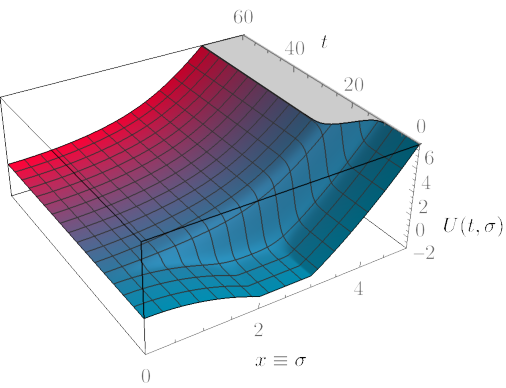
\includegraphics[width=5.5cm]{0d/figures/sc_i_on_3_n_800_xmax_10_lambda_1e6_tir_60_rg_flow_u_3d.pdf}
		\caption{Three-dimensional rendering of the flow $U(t,\sigma)$ displayed on the left \dash{} \Cref{fig:sc_i_on_3_n_800_xmax_10_lambda_1e6_tir_60_rg_flow_2d} (upper panel).}%
		\label{fig:sc_i_on_3_n_800_xmax_10_lambda_1e6_tir_60_rg_flow_u_3d}%
	}% figure/caption/label (b)
	{%
		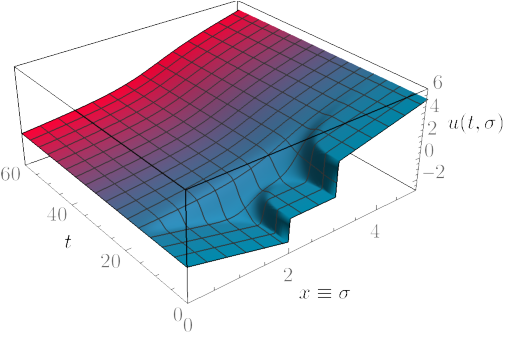
\includegraphics[width=5.5cm]{0d/figures/sc_i_on_3_n_800_xmax_10_lambda_1e6_tir_60_rg_flow_du_3d.pdf}
		\caption{Three-dimensional rendering of the flow $u(t,\sigma)$ displayed on the left \dash{} \Cref{fig:sc_i_on_3_n_800_xmax_10_lambda_1e6_tir_60_rg_flow_2d} (lower panel).}%
		\label{fig:sc_i_on_3_n_800_xmax_10_lambda_1e6_tir_60_rg_flow_du_3d}%
	}% figure/caption/label (c)
	{%
	The \frg{} flow of the effective potential $U ( t, \sigma )$ \dash{} upper panel/figure on the left~\subref{fig:sc_i_on_3_n_800_xmax_10_lambda_1e6_tir_60_rg_flow_2d} and on the right~\subref{fig:sc_i_on_3_n_800_xmax_10_lambda_1e6_tir_60_rg_flow_u_3d} \dash{} and its derivative $u ( t , \sigma ) = \partial_\sigma U ( t , \sigma )$ \dash{} lower panel/figure on the left~\subref{fig:sc_i_on_3_n_800_xmax_10_lambda_1e6_tir_60_rg_flow_2d} and on the right~\subref{fig:sc_i_on_3_n_800_xmax_10_lambda_1e6_tir_60_rg_flow_du_3d} \dash{} for the zero-dimensional $O ( 3 )$ model with initial condition \eqref{eq:testing_scenario_non-analytic_quadaratic_asymptote}. 
	The blue curves correspond to the \uv{} and the red curves to the \ir{}.
	We used the exponential regulator~\eqref{eq:exponential_regulator} with \uv{} scale $\Lambda = 10^6$.
	For the sake of readability, the plots do not show the region ${x \in[5,10]}$, because the tiny differences between $u ( t , \sigma )$ and $u ( 0 , \sigma )$ are not visible in this region and vanish for large $x = \sigma$ anyhow.
	\fromFigs{5, 6, and 7}{zerod1}%
	}% caption
	{fig:sc_i_on_3_n_800_xmax_10_lambda_1e6_tir_60_rg_flow}% label
We start our analysis with a general discussion of the \frg{} flow with \ic{} \eqref{eq:testing_scenario_non-analytic_quadaratic_asymptote}.
To this end, we fix $O(N = 3)$ to include both diffusive and advective contributions via the radial \sigmaMode{} and two pions. For $N = 3$ the number of pions is reasonably small and the (diffusive) effects of the \sigmaMode{} remain visible.
Furthermore, we choose $[ 0, x_\mathrm{max} = 10 ]$ as the spatial computational domain with $n=800$ volume cells and use the \ktScheme{} from \cref{subsec:hydroKT} for spatial discretization.
The initial cell averages $\bar{u}_i ( t = 0 )$ are computed by exact averaging\footnote{%
	Using the exact averages for $\bar{u}_i(t=0)$ has proven advantageous in terms of achievable numerical precision in the \ir{} compared to taking the mid-point values of the exact derivative of ${ \bar{u}_i ( t = 0 ) = \partial_\sigma U ( \sigma ) |_{\sigma = \sigma_i} }$ when considering non-analytic \ics{} like \cref{eq:testing_scenario_non-analytic_quadaratic_asymptote} or \eqref{eq:testing_scenario_4}.%
} 
\begin{align}
	\bar{u}_i ( t = 0 ) = \frac{1}{\Delta \sigma} \, \big[ U \big( \sigma_{i + \frac{1}{2}} \big) - U \big( \sigma_{i - \frac{1}{2}} \big) \big] ,
\end{align}
using the \uv{} \ic{} \eqref{eq:testing_scenario_non-analytic_quadaratic_asymptote}.
We use linear extrapolation \eqref{eq:BClinExt} as spatial \bc{} at $x_\mathrm{max}$ as discussed in \cref{paragraph:BCinf}.
The \uv{} scale is set to $\Lambda = 10^6$ at $t = 0$. 
Time evolution of the semi-discrete \kt{} \ode{} system is performed with \textit{NDSolve} of \WAMXIIwR{} with a \textit{PrecisionGoal} and \textit{AccuracyGoal} of 10 and stopped in the \ir{} at $r ( t_\mathrm{IR} = 60 ) \approx 10^{-20}$ using the exponential regulator shape function \eqref{eq:exponential_regulator}.
Time-stepping has not been a focus of our work and we refer the interested reader to the excellent \ccite{Ihssen:2023qaq} discussing the issue in the context of \frg{} in detail.
We find that this choice of parameters suffices to produce decent results, as discussed in the following.
There, we quantitatively analyze sources and severity of possible errors related to those (numerical) parameters.

We first provide qualitative results of our numerical methods in \cref{fig:sc_i_on_3_n_800_xmax_10_lambda_1e6_tir_60_rg_flow}, where we show the \frg{} flow of the effective potential $U ( t, \sigma )$ and its derivative $u ( t, \sigma ) = \partial_\sigma U ( t, \sigma )$ from the \uv{} (blue) to the \ir{} (red).
In the beginning, \ie{}, in the \uv{}, the system is in the broken phase. 
This changes only marginally until $t \approx 7$, which indicates that the \uv{} scale is chosen sufficiently large with $\Lambda = 10^6$.
When $r(t)$ reaches the scales of the model at $t \smallergtrsim 11$ most of the dynamics takes place (symmetry restoration) and $u ( t, \sigma )$ changes rapidly and drastically until it freezes out in the \ir{}.
In the \ir{} the system is in the restored phase as expected \apriori{}.
After $t \approx 26$ the potential does not change anymore, which indicates that one has reached a sufficiently small \ir{} scale to stop the integration.
We render this statement more precise in the following \cref{paragraph:ONRGconsistency}.
Note that the evolution in $t$ is logarithmic and corresponds to a change in scale over $25$ orders of magnitude.
At first glance this range sounds excessive, but its necessity is explained in detail in \cref{paragraph:ONRGconsistency}.

During the \frg{} evolution one observes that diffusive processes smear out the discontinuities at the non-analytic points at $\sigma = 2$ and $\sigma = 3$.
We also find that the diffusion acts in both directions \dash{} towards larger and smaller values of $\sigma$ \dash{} as expected from our discussion in \cref{subsubsec:conservative_form}. 
Nevertheless, the diffusive effects do not reach the computational boundary, which is outside the plot range at $\sigma_\mathrm{max} = 10$.
This suggests that $\sigma_\mathrm{max} = 10$ is sufficiently large.
Additionally, we observe a propagation of the conserved quantity $u$ towards smaller values of $\sigma$ via advection. 
Close to the initial discontinuities these advective processes can be interpreted as rarefaction waves. 
In a more pictorial language, the advection and diffusion ``fill up the pit'' in $u ( t, \sigma )$ at small values of $\sigma$ by moving more and more of the quantity $u$ from larger values of $\sigma$ to smaller $\sigma$ (via advection and diffusion) as well as from small negative $\sigma$ to small positive $\sigma$ (via diffusion).
Eventually the symmetry is restored and $u ( t, \sigma )$ is smoothed towards the \ir{} by diffusion. 
Furthermore, the conserved quantity $u$ does not ``pile up'' at $\sigma = 0$ after symmetry restoration, because at negative $\sigma$ exactly the opposite dynamics happens, due to the \ZII{} antisymmetry of $u ( t, \sigma )$, which is encoded in the \bc{} at $\sigma = 0$, see \cref{subsec:boundary_conditions_finite_volume}.
The differences between advective and diffusive contributions become apparent when comparing the same system for different $N$, \cf{} \cref{fig:sc_i_on_1_10_100_n_800_xmax_10_lambda_1e6_tir_60_rg_flow} and the surrounding discussion.

From a numerical perspective, the \ktScheme{} is able to handle the highly non-linear dynamics, including the non-analyticities in $u ( t, \sigma )$, without any spurious oscillatory behavior (under-/over-shooting) and allows for a stable $t$ integration to extremely small \ir{} scales.

For the sake of completeness and illustrative purposes, we also provide the \frg{} flow of the integral of $u ( t, \sigma )$, \ie{}, the effective potential $U ( t, \sigma )$, in \cref{fig:sc_i_on_3_n_800_xmax_10_lambda_1e6_tir_60_rg_flow_2d} (upper panel) and \cref{fig:sc_i_on_3_n_800_xmax_10_lambda_1e6_tir_60_rg_flow_u_3d}.
Here, the integration constant was set to zero\footnote{%
	$U ( t, 0 ) = 0$ is dictated by our choice of normalization for the zero-point function(s), see \cref{eq:normalization}.
} and the integration was performed via Riemann summation\footnote{%
	At this point we should mention that numerical results for $U ( t, \sigma )$ via Riemann summation should be treated with great caution: Numerical errors in the cell averages $\bar{u} ( t, x_j )$ which arise from the numerical \frg{} flow can accumulate during integration (here summation) along $\sigma = x$.
	More precise quadrature methods should be used if precise, quantitative values for $U ( t, \sigma )$ are needed.
} of the discrete cell averages,
	\begin{align}
		U ( t, x_i ) = \Delta x \sum_{j = 0}^{i} \frac{\bar{u} ( t, x_j )}{( 1 + \delta_{j, 0} + \delta_{j, i} )} \, .	\label{eq:riemann_sum}
	\end{align}
\Cref{fig:sc_i_on_3_n_800_xmax_10_lambda_1e6_tir_60_rg_flow_u_3d} perfectly illustrates the restoration of the $O(3)$ symmetry of the potential $U ( t, \sigma )$ during the \frg{} flow via ``vaporization'' of the infinitely many minima.
Nevertheless, we find that it is hardly possible to intuitively understand the contributions of the radial \sigmaMode{} and the pions to the \frg{} flow on the level of $U ( t, \sigma )$ only.
This complements the discussion in \cref{subsubsec:conservative_form} and lends support to our claim that the fluid-dynamical interpretation of the \frg{} flow in terms of $u ( t, \sigma )$ is superior to the canonical formulation in terms of $U ( t, \sigma )$ commonly used in the \frg{} literature.

\WarningFilter{latex}{Text page}
\fullWidthTwoColumnFigures%
	[!t] % Placement
	{%
		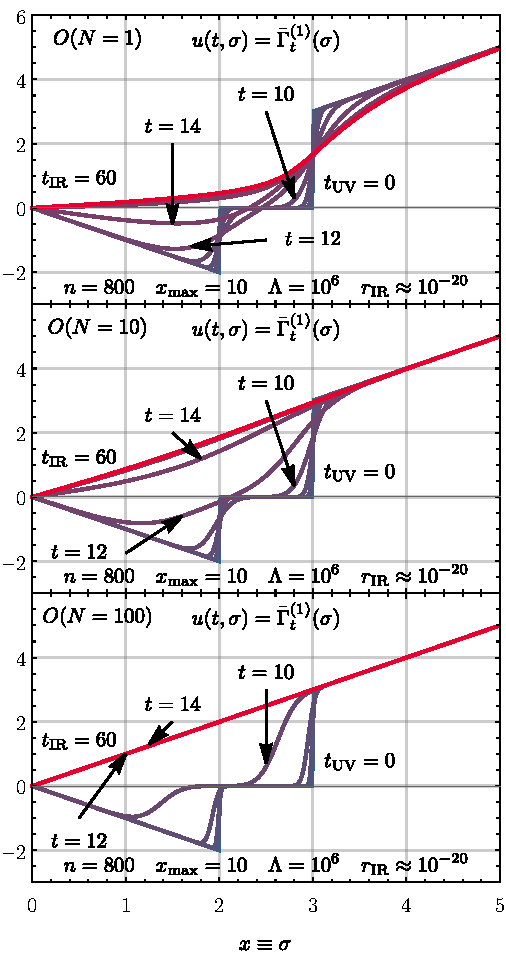
\includegraphics[width=\subcaptionFigureWidth-0.2cm]{0d/figures/sc_i_on_1_10_100_n_800_xmax_10_lambda_1e6_tir_60_rg_flow.pdf} % left figure
		\captionsetup{width=\subcaptionFigureWidth}%
		\caption{%
			The \frg{} flow of the derivative of the effective potential $u ( t , \sigma ) = \partial_\sigma U ( t, \sigma )$ for the zero-dimensional $O(N)$ model for $N = 1, \, 10, \, 100$ with \ic{} \eqref{eq:testing_scenario_non-analytic_quadaratic_asymptote}.
			All other parameters are identical to those in \cref{fig:sc_i_on_3_n_800_xmax_10_lambda_1e6_tir_60_rg_flow}.
			\fromFig{8}{zerod1}
		}
		\label{fig:sc_i_on_1_10_100_n_800_xmax_10_lambda_1e6_tir_60_rg_flow}
	}
	{\fullWidthTwoColumnFigureSpacing}
	{%
		\vspace{.065cm}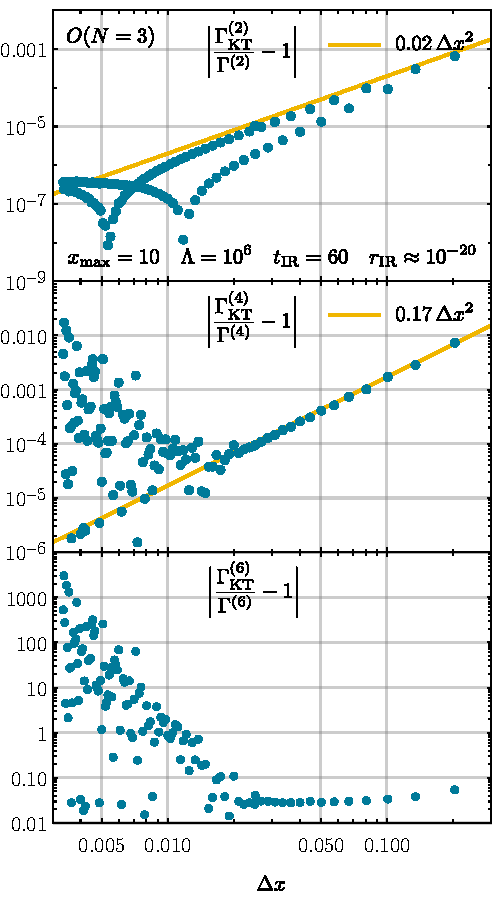
\includegraphics[width=\subcaptionFigureWidth+0.2cm]{0d/figures/sc_i_on_3_xmax_10_lambda_1e6_tir_60_deltax_scaling.pdf} % Right figure
		\captionsetup{width=\subcaptionFigureWidth}%
		\caption{%
			The relative error of the numerical results (blue dots) from the \kt{} scheme for the \ipi{} \nptFunctions{} $\Gamma^{(2n)}$ for $n = 1, 2, 3$ as a function of $\Delta x$ with \ic{} \eqref{eq:testing_scenario_non-analytic_quadaratic_asymptote}.
			The numerical derivatives at $\sigma = 0$ of $u(t_\mathrm{IR}=60, \sigma)$ were calculated via the second-order accurate central schemes \eqref{eq:derivative_1_central_error_2}, \eqref{eq:derivative_3_central_error_2}, and \eqref{eq:derivative_5_central_error_2}.
			The plot was produced with $x_\mathrm{max} = 10$, but could have been calculated for any sufficiently large $x_\mathrm{max}$.
			We used the exponential regulator~\eqref{eq:exponential_regulator} with \uv{} scale $\Lambda = 10^6$.
			The yellow straight lines $\propto \Delta x^2$ are for optical guidance.
			\fromFig{9}{zerod1}%
		}%
		\label{fig:sc_i_on_3_xmax_10_lambda_1e6_tir_60_deltax_scaling}
		\vspace{1cm}
	}%
\WarningFilter*{latex}{Text page}
Before discussing quantitative results and sources of (numerical) errors in \frg{} flows, we briefly return to the interpretation of the radial \sigmaMode{} as diffusion and the interpretation of the pions as advection in the \frg{} flow along the field space direction.
To this end, we discuss \frg{} flows for the same \uv{} initial potential \eqref{eq:testing_scenario_non-analytic_quadaratic_asymptote} as before, but for different $N$.
This  corresponds to a different number of pions in the flow and different advection velocities \eqref{eq:advection_velocity}.
All other parameters remain unchanged.
In addition to the $N = 3$ case in \cref{fig:sc_i_on_3_n_800_xmax_10_lambda_1e6_tir_60_rg_flow}, we provide the \frg{} flows of $u ( t, \sigma )$ for $N = 1, 10, 100$ in \cref{fig:sc_i_on_1_10_100_n_800_xmax_10_lambda_1e6_tir_60_rg_flow}.
The figure again demonstrates on a qualitative level that the \sigmaMode{} enters the \frg{} as diffusion, while pions enter as advection: Increasing the number of pions the problem becomes more advection-driven exhibiting more pronounced waves and faster propagation.
This can be seen by comparing the plots at equal \rgtimes{}.
For $N = 1$, the problem reduces to the pure diffusion equation \eqref{eq:pde_gamma}, where the dynamics is slowest and the diffusion propagates the fluid from negative $\sigma$ to small positive $\sigma$ close to $\sigma = 0$.
Furthermore, one observes stronger smearing of the discontinuities at $\sigma = 2$ and $\sigma = 3$.
The $N = 100$ case is extremely advection-dominated.
In the fluid-dynamical language, this corresponds to a complete suppression of diffusion, which is clearly observed from the fast propagation of the rarefaction waves and almost negligible smoothing of the discontinuities at $\sigma = 2$ and $\sigma = 3$.
We will discuss the qualitative and quantitative differences between \frg{} flows at small $N$ with flows large and even infinite $N$ in \cref{subsec:0dLargeN}.

\paragraph{Tests of the spatial resolution}\phantomsection\label{paragraph:ONdeltax}\mbox{}\\%
This paragraph is dedicated to quantifying numerical errors in the \frg{} flow arising from the finite spatial resolution $\Delta x\equiv \Delta \sigma$ of the cells in the \ktScheme{}.
Any spatial discretization comes with a discretization error.
The \ktScheme{}, which is used throughout this thesis, is formally of second-order accuracy in $\Delta x$ when employing the numerical fluxes of \cref{eq:FVKTO2} with the five-point stencil \eqref{eq:kt_stencil}.
Therefore, the numerical errors arising from the spatial discretization should scale with $\Delta x^2$ when $\Delta x$ is decreased.

As test values (observables) we use the modulus of the relative errors of the \ipi{} \nptFunctions{} $\Gamma^{(2n)}$ for $n = 1, 2, 3$,
\begin{align}
	\bigg| \frac{\Gamma^{(2n)}_\mathrm{KT}}{\Gamma^{(2n)}} - 1 \bigg| \, ,	\label{eq:relative_errors_gamma_2n}
\end{align}
where $\Gamma^{(2n)}_\mathrm{KT}$ is calculated from the \frg{} (via the \ktScheme{}) and $\Gamma^{(2n)}$ from the integral, see \cref{tab:sc_1_n_point_functions_exact}.
In order to determine how much of the relative numerical error~\eqref{eq:relative_errors_gamma_2n} is directly related to the spatial discretization, we have to optimize all other parameters of the computation in order to reduce other sources of errors.
We basically choose the same parameter set \dash{} \viz{} $\Lambda = 10^6$, $x_\mathrm{max} = 10$ and $t_\mathrm{IR} = 60$ \dash{} and \uv{} \ic{} \eqref{eq:testing_scenario_non-analytic_quadaratic_asymptote} which was also used for the qualitative analysis in the previous paragraph and only vary the number of cells $n$ to change the resolution $\Delta x$.
\WlogA{} we keep $N=3$.

Before we embark on our discussion, we remark that the spatial-discretization error enters the relative errors~\eqref{eq:relative_errors_gamma_2n} in a twofold way: 
\begin{enumerate}
	\item	There is the discretization error which comes from the \ktScheme{} during the \frg{} time integration.
	This error shows up directly in the \ir{} values $u ( t_\mathrm{IR}, x_i )$ and should scale according to $\Delta x^2$ for the chosen second-order \ktScheme{}.

	\item	There is a discretization error which is related to the extraction of the \ipi{} \nptFunctions{} from the discrete $\bar{u} ( t_\mathrm{IR}, x_i )$. 
	They have to be calculated at the physical point (the minimum at $x = \sigma = 0$) via numerical differentiation, which also comes with a discretization error.
	The latter is also related to the spatial resolution $\Delta x$.
	In general (especially in higher-dimensional models) it is not clear whether these numerical derivatives at the physical point are always well-defined.
	We argued before that $u ( t, \sigma )$ might exhibit non-analytical behavior also at the physical point in the \ir{}, \cf{}\ \ccite{Grossi:2019urj,Grossi:2021ksl,Borchardt:2016pif,Stoll:2021ori}, such that a naive numerical differentiation is not allowed in general.
	In the special case of zero-dimensional \qfts{}, we proved in \MWApp{} that the \ir{} effective action and the \ir{} potential $U ( t \rightarrow \infty, \vec{\varphi}\, )$ are smooth, which also translates to $u ( t \rightarrow \infty, \sigma )$, such that numerical differentiation (\eg{}, via finite-difference approximations) is well-defined.
\end{enumerate}
However, even though finite-difference formulas are reliable approximations for derivatives of a smooth function and have a well-defined truncation-error scaling in powers of $\Delta x$, there remains a well-known subtlety: While decreasing the resolution $\Delta x$, one eventually will reach a point where the error starts increasing again contrary to the formal truncation-error scaling. 
This is related to the ill-conditioned nature of finite-difference formulas and to explicit rounding errors in floating-point arithmetic, which increase the error of the numerical derivative below a certain $\Delta x$, see, \eg{}, Chap.~5.7 of \ccite{PresTeukVettFlan92}.
Related spurious cancellations occur if the discrete data of a smooth function include some sort of noise.
In our case this ``noise'' is directly related to the spatial-discretization errors from the \ktScheme{} and the errors from \rgtime{} integration using numerical \ode{} solvers.
These errors might be tiny, but can easily inflate the errors of the numerical derivatives, especially for higher-order derivatives.

In conclusion, while decreasing $\Delta x$, we expect that long before the relative errors from the \ktScheme{} start increasing again (because the \ktScheme{} begins operating close to machine precision or because the error of the time stepping becomes relevant) the relative errors \eqref{eq:relative_errors_gamma_2n} start increasing due to the numerical differentiation of slightly ``noisy data''. 
This phenomenon is expected to set in at larger $\Delta x$ for approximations for higher-order derivatives and long before the formal error scaling of the \ktScheme{} is no longer valid.

Our explicit results for the scaling of the relative errors with decreasing spatial resolution are presented in \cref{fig:sc_i_on_3_xmax_10_lambda_1e6_tir_60_deltax_scaling}, where we show the relative errors \eqref{eq:relative_errors_gamma_2n} for the \hbox{two-}, \hbox{four-}, and six-point functions in a double-logarithmic plot over $\Delta x$.
For $\Gamma^{(2)}$ and $\Gamma^{(4)}$ we find that the corresponding relative errors scale with $\Delta x^2$ (or even slightly better) as expected from the error scaling of the \ktScheme{} as well as the error scaling of the finite-difference stencils~\eqref{eq:derivative_1_central_error_2} and \eqref{eq:derivative_3_central_error_2}.
We observe two groups of points for $\Gamma^{(2)}$ (upper panel of \cref{fig:sc_i_on_3_xmax_10_lambda_1e6_tir_60_deltax_scaling}), which are related to discretization errors of the discontinuous \ic{} \eqref{eq:testing_scenario_non-analytic_quadaratic_asymptote} at $x=2$ and $x=3$. 
The error scaling of $0.02\, \Delta x^2$ for $\Gamma^{(2)}$ is a conservative estimate for the observed errors, which are actually lower for $\Delta x \smallergtrsim 0.005$. 
For $\Delta x \smallerlesssim 0.005$ we observe deviations from the conservative estimate for the error scaling of $\Gamma^{(2)}$ related to other error sources.
In the middle panel of \cref{fig:sc_i_on_3_xmax_10_lambda_1e6_tir_60_deltax_scaling}, we clearly see that there is an optimal minimal $\Delta x \approx 0.02$ where the correct formal scaling of the numerical derivative breaks down and the relative error of $\Gamma^{(4)}$ increases again for smaller $\Delta x$.
We can be sure that this breakdown of the error scaling is related to the numerical differentiation and not the \ktScheme{} because we observe scaling with at least $\Delta x^2$ for $\Gamma^{(2)}$ in the upper panel of \cref{fig:sc_i_on_3_xmax_10_lambda_1e6_tir_60_deltax_scaling} well below $\Delta x \approx 0.02$.
This is expected for lower-order numerical derivatives.
Furthermore, we find that for $\Gamma^{(6)}$ (lower panel of \cref{fig:sc_i_on_3_xmax_10_lambda_1e6_tir_60_deltax_scaling}) the order of the numerical derivative is already too large, such that the theoretical error scaling of the \ktScheme{} cannot be seen at all and is completely obscured by the errors from the numerical differentiation of $\bar{u} ( t_\mathrm{IR}, x_i )$.

We conclude that the \ktScheme{} is perfectly suited for the spatial discretization of the \frg{} flow equation for $u ( t, \sigma )$ and shows correct scaling with decreasing spatial resolution $\Delta x$. 
This is also confirmed by tests with different \ics{}, see, \eg{}, \cref{fig:sc_ii_n_on_4_xmax_10_lambda_1e12_tir_60_deltax_scaling}.

In addition, we actually found that a more severe problem is the correct extraction of physical observables from the \ir{} values $\bar{u} ( t_\mathrm{IR}, x_i )$, which are usually related to derivatives of $u ( t_\mathrm{IR}, \sigma )$.
We predict that this problem might even become more severe in higher dimensions, were the \ir{} potential is no longer guaranteed to be smooth.
We therefore suggest to search for better ways of calculating those derivatives as well as for careful analysis tools for numerically calculated \ipi{} \nptFunctions{} in the vicinity of non-analyticities in general.
However, this is beyond the scope of the present work.

We remark that our numerical findings indicate that \dash{} independent of the specific numerical discretization scheme \dash{} the number of grid points or expansion coefficients might have been chosen too small in previous \frg{} studies in literature to obtain a decent resolution.
However, other works, \cf{} \ccite{Pelaez:2015nsa,Caillol:2012zz,Pangon:2009pj,Pangon:2010uf,Borchardt:2015rxa,Borchardt:2016pif}, which also discuss the limitations of their numerical schemes in detail, have used a rather large number of discretization points \dash{} in some cases to compensate the demand for continuity of the specific schemes.

In the following we will mostly use a spatial resolution of 
	\begin{align}
		\Delta x = \frac{x_\mathrm{max}}{n - 1} \simeq 0.025 \, ,
	\end{align}
where we can trust the results for the two- and four-point functions.
The relative errors for the six-point function will only be plotted for the sake of completeness, but cannot be included in any reasonable quantitative analysis of other sources of (numerical) errors in \frg{} flow equations although they are still at a reasonably small level of $\sim 5\%$ at $\Delta x \simeq 0.025$.

\paragraph{Tests of the size of the computational domain}\phantomsection\label{paragraph:test_size_computational_domain}\mbox{}\\%
\fullWidthTwoColumnSubFigures%
	[!t]% Placement
	{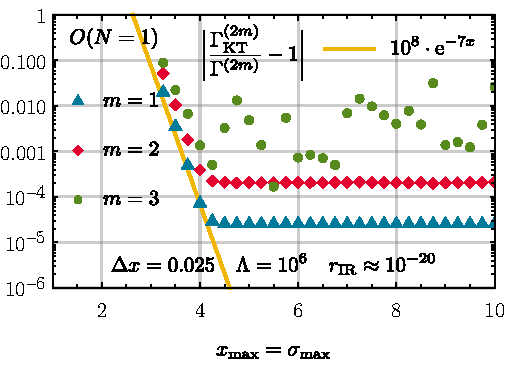
\includegraphics[width=\subcaptionFigureWidth]{0d/figures/sc_i_on_1_deltax_25e-3_lambda_1e6_tir_60_errors_xmax.pdf}}% Left figure (dummy index a)
	{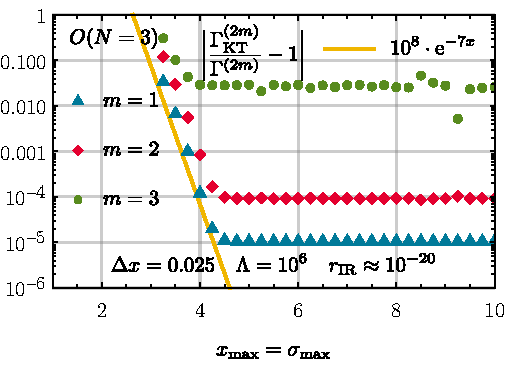
\includegraphics[width=\subcaptionFigureWidth]{0d/figures/sc_i_on_3_deltax_25e-3_lambda_1e6_tir_60_errors_xmax.pdf}}% Right figure (dummy index b)
	[fig:sc_i_on_1_deltax_25e-3_lambda_1e6_tir_60_errors_xmax,fig:sc_i_on_3_deltax_25e-3_lambda_1e6_tir_60_errors_xmax] %Labels
	{%
		The relative error for $\Gamma^{(2m)}$ for $m = 1, 2, 3$ for the \uv{} potential \eqref{eq:testing_scenario_non-analytic_quadaratic_asymptote} of the \ONn{1} model on the left \subref{fig:sc_i_on_1_deltax_25e-3_lambda_1e6_tir_60_errors_xmax} and of the \ONn{3} model on the right \subref{fig:sc_i_on_3_deltax_25e-3_lambda_1e6_tir_60_errors_xmax} as a function of $x_\mathrm{max}$, while keeping the cell size constant, $\Delta x = 0.025$. $\Gamma^{(2m)}$ are computed from the discrete values of the derivative of the \ir{} potential $u ( t_\mathrm{IR} = 60, \sigma )$ via the second-order accurate central finite-difference stencils~\eqref{eq:derivative_1_central_error_2}, \eqref{eq:derivative_3_central_error_2}, and \eqref{eq:derivative_5_central_error_2} at $\sigma = 0$.
		We use the exponential regulator~\eqref{eq:exponential_regulator} with \uv{} scale $\Lambda = 10^6$.
		The yellow straight line $\propto\exp{-7x_\mathrm{max}}$ is for optical guidance.
		\fromFigs{10 and 11}{zerod1}%
	}% Caption
	{fig:sc_i_on_deltax_25e-3_lambda_1e6_tir_60_errors_xmax}% Label
In this paragraph, we discuss the influence of the size of the computational domain $[ 0, \sigma_\mathrm{max} ]$ on the relative errors of the \ir{} observables \eqref{eq:relative_errors_gamma_2n}.
As discussed in \cref{subsec:boundary_conditions_finite_volume}, we expect that, if the spatial \bcs{} are not implemented with great caution and the computational domain is too small, one cannot trust the results from the numerical integration of the \frg{} flow.
If the computational domain is too small, we expect large errors, because the \bcs{} at $\sigma_\mathrm{max}$ are no longer valid due to wrong extrapolation to the ghost cells and consequently wrongly estimated influx.

In the case with \uv{} \ic{} \eqref{eq:testing_scenario_non-analytic_quadaratic_asymptote}, the \bc{} at $\sigma_\mathrm{max}$ is implemented as a linear extrapolation \eqref{eq:BClinExt} of $u ( t, \sigma )$ to the two ghost cells of the \ktScheme{} to mimic the asymptotic behavior of $u ( t, \sigma )$. 
As long as $\sigma_\mathrm{max}$ is sufficiently large, we expect only tiny deviations of $u ( t, \sigma )$ from its initial \uv{} value $u ( t_\mathrm{UV} = 0, \sigma )$ around $\sigma_\mathrm{max}$.
However, if $\sigma_\mathrm{max}$ is too small and approaches the model scales, we expect the diffusive effects to reach the boundary of the computational domain, such that a linear extrapolation is no longer a good approximation in order to determine the spatial \bc{}.

To this end, we test the scaling of the relative errors \eqref{eq:relative_errors_gamma_2n} with decreasing computational domain size $x_\mathrm{max} = \sigma_\mathrm{max}$ for $N = 1$ (purely diffusive) and $N = 3$. 
The results and (numerical) parameters are shown in \cref{fig:sc_i_on_deltax_25e-3_lambda_1e6_tir_60_errors_xmax}.
In both cases ($N=1$ and $N=3$ in \cref{fig:sc_i_on_1_deltax_25e-3_lambda_1e6_tir_60_errors_xmax,fig:sc_i_on_3_deltax_25e-3_lambda_1e6_tir_60_errors_xmax} respectively) we find that the relative errors are independent of $\sigma_\mathrm{max}$ for sufficiently large $\sigma_\mathrm{max}$.
However, if the spatial cutoff $\sigma_\mathrm{max}$ is approaching the model scales (here the discontinuity in $u ( t_\mathrm{UV} = 0, \sigma )$ at $\sigma = 3$, see \cref{fig:sc_i_uv_initial_condition}) the relative errors for $\Gamma^{(2)}$ and $\Gamma^{(4)}$ start rising exponentially.

Contrary to our expectations, the results for $N = 1$ and $N = 3$ are very similar and the exponential rise of the relative errors sets in at a similar $\sigma_\mathrm{max}\approx 4.2$.
\Apriori{} we expected that for the purely diffusive scenario with $N = 1$, the diffusive effects arising from the large gradients at $\sigma = 3$ might have more time to reach and influence the shape of $u ( t, \sigma )$ at larger values of $\sigma$, which does not seem to be the case.
Our employed monitors for numerical errors \dash{} the \ipi{} \nptFunctions{} in the \ir{} computed at $\sigma=0$ and $t=0$ \dash{} are rather intensive to such changes.
A possible explanation is the fact that observable errors from the boundary at $\sigma_\mathrm{max}$ propagate into the computational domain at a finite speed\footnote{
	In the context of ``infinite propagation speeds'' in parabolic \pdes{}, \cf{} the discussion and corresponding footnote~\ref{footnote:HEinf} in \cref{subsec:hydroDiffusion}, we refer here to the fact that observable changes on the relevant scales of the problem travel with apparently finite speed independent from some formal instantaneous, infinitesimal (exponentially decaying) changes.% 
}, which is rather low in the purely diffusive case and in general small at large~$\sigma$, and thus do not influence the physical point at $t=0$ and $\sigma=0$. 

Nevertheless, we conclude from \cref{fig:sc_i_on_1_deltax_25e-3_lambda_1e6_tir_60_errors_xmax,fig:sc_i_on_3_deltax_25e-3_lambda_1e6_tir_60_errors_xmax} that it is extremely important to use sufficiently large computational domains to minimize numerical errors in field-dependent \frg{} flows. 
This implies that $\sigma_\mathrm{max}$ should be chosen much larger than all relevant scales of the model.

\fullWidthTwoColumnSubFigures
	[!t] % Placement
	{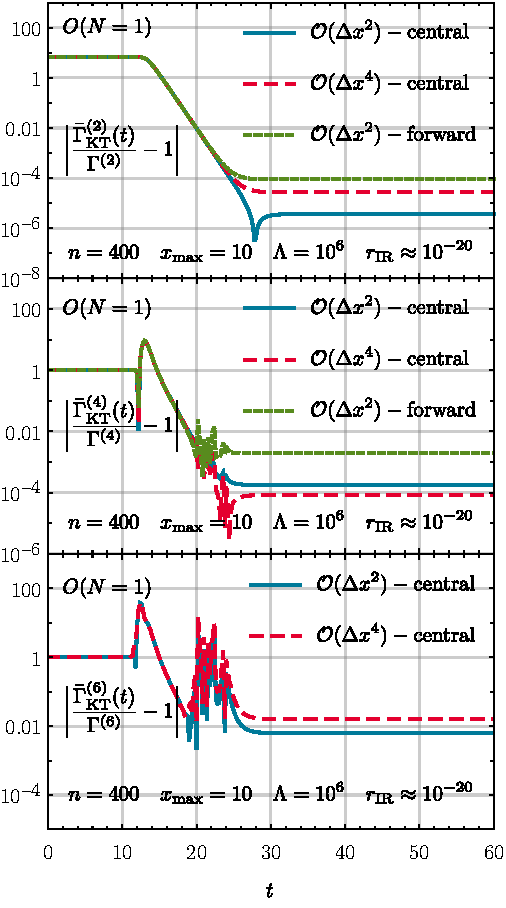
\includegraphics[width=\subcaptionFigureWidth]{0d/figures/sc_i_on_1_n_400_xmax_10_lambda_1e6_tir_60_flow_errors.pdf}} % left figure (dummy index a)
	{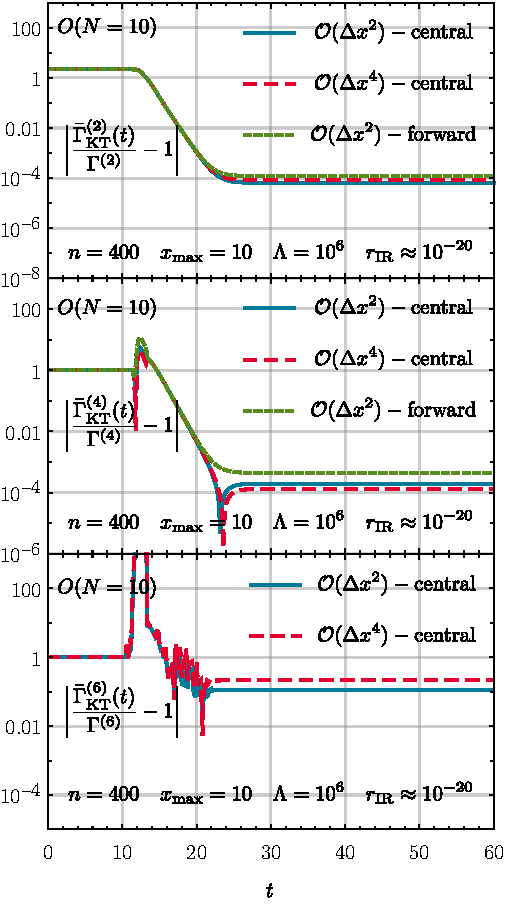
\includegraphics[width=\subcaptionFigureWidth]{0d/figures/sc_i_on_10_n_400_xmax_10_lambda_1e6_tir_60_flow_errors.pdf}} % Right figure (dummy index b)
	[fig:sc_i_on_1_n_400_xmax_10_lambda_1e6_tir_60_flow_errors,fig:sc_i_on_10_n_400_xmax_10_lambda_1e6_tir_60_flow_errors] %Labels
	{%
		The relative error for $\Gamma^{(2m)}$, for $m = 1, 2, 3$, calculated with the \kt{} scheme as a function of the \rgtime{} $t$ for the \ONn{1} model on the left~\subref{fig:sc_i_on_1_n_400_xmax_10_lambda_1e6_tir_60_flow_errors} and of the \ONn{10} model on the right~\subref{fig:sc_i_on_10_n_400_xmax_10_lambda_1e6_tir_60_flow_errors}.
		The \uv{} initial potential is given by \cref{eq:testing_scenario_non-analytic_quadaratic_asymptote}. 
		We use the exponential regulator~\eqref{eq:exponential_regulator} with \uv{} scale $\Lambda = 10^6$. 
		The computational grid has $n=400$ cells and $\sigma_\mathrm{max} = x_\mathrm{max} = 10$. $\Gamma^{(2m)}$ are extracted from $u ( t_\mathrm{IR} = 60, \sigma )$ via the finite-difference stencils \eqref{eq:derivative_1_central_error_2}\dash{}\eqref{eq:derivative_5_central_error_4}.
		\fromFigs{13 and 15}{zerod1}
	} % Caption
	{fig:sc_i_on_n_400_xmax_10_lambda_1e6_tir_60_flow_errors} % Label
From our findings, it is therefore expected that choosing a large $\sigma_\mathrm{max}$ might even gain in importance in higher-dimensional models, where the physical point may be located at a non-trivial minimum in the \ir{}, like in the \qm{} and \gnyBm{} of \cref{chap:GN,chap:QMM}. 
If the physical point is closer to the boundary of the computational domain the relative errors for observables might even be larger than for our zero-dimensional model where the physical point moves towards $\sigma = 0$ during the \frg{} flow. 
In terms of errors originating from the boundary at $\sigma_\mathrm{max}$, the physical point at $\sigma = 0$ is ideal since it has the largest spatial and \dash{} in a sense causal, due to the finite speed of propagation \dash{} distance to $\sigma_\mathrm{max}$.

Lastly, we have to warn that there is no panacea for the construction of a sufficiently large computational domain and the choice of $\sigma_\mathrm{max}$ has to be adjusted to the specific model and specific \ic{} under consideration. 
For some problems even more involved approaches (like using several computational grids of different resolution $\Delta x$) might be needed or are at least highly advantageous~\cite{Grossi:2019urj,Grossi:2021ksl,Ihssen:2022xkr,Ihssen:2023xlp}.
In any case one has to check that the \ir{} results do not depend on the size of the computational domain (even if exact reference values for observables are unknown), \cf{} \ccite{Pangon:2009pj,Caillol:2012zz,Stoll:2021ori}.
This can be done by fixing appropriate values for the spatial resolution $\Delta x$ as well as for all other (numerical) parameters and successively increasing $\sigma_\mathrm{max}$ until the \ir{} observables do not change anymore.

\paragraph{Tests of the \uv{} and \ir{} scales}\phantomsection\label{paragraph:ONRGconsistency}\mbox{}\\%
We now turn to a long-standing discussion in the \frg{} community, namely the question: How do we have to choose the initial \uv{} and numerical \ir{} cutoff scale for the calculation of the 
\frg{} flow for a specific model? 

A common argument is based on the energy scales of a given model. The \uv{} \ic{} is fixed at \uv{} scales $\Lambda$ that are close to the largest energy scale of the model.
Higher $\Lambda$ are excluded by arguing that at higher energy scales other physical degrees of freedom (\eg{}, other interaction channels or new particles) are relevant and the model at hand is only valid within a certain energy regime.
On the other hand, the \ir{} cutoff $k_\mathrm{IR}$ scale is oftentimes fixed by arguing that if it decreases below the lowest energy scale of the model, the \frg{} flow is effectively ``frozen in'' and the effective potential no longer changes anyway.
A relatively low \uv{} initial scale and a high \ir{} cutoff lead to rather short flow times of only $t_\mathrm{UV} - t_\mathrm{IR} \approx 3 - 4$.

Another approach, which is sometimes employed in conjunction with the first strategy, is guided by the principle of ``numerical stability'' of the \frg{} flow, where cutoffs are chosen in a certain way to ``improve performance and stability'' during the numerical \rgtime{} integration.
In turn, in \ccite{Pelaez:2015nsa,Caillol:2012zz,Pangon:2009pj,Pangon:2010uf,Borchardt:2016pif} relatively small \ir{} cutoff scales are reached due to the use of numerical stable schemes or the control of stability.
Careful extrapolations into the deep \ir{} like the ones discussed in, \eg{}, \ccite{Pelaez:2015nsa,Grossi:2019urj,Grossi:2021ksl} are another possibility to achieve low \ir{} cutoffs.
Note that, for theories in $d>0$ dimensions, numerical integration into the (deep) \ir{} becomes very demanding due to multiple reasons, see also \ccite{Pelaez:2015nsa,Grossi:2019urj,Grossi:2021ksl,Stoll:2021ori} and especially \ccite{Ihssen:2023qaq}.
This is probably the main reason why often large numerical \ir{} cutoffs are used.

In general, however, there is a well-defined strategy for the choice of the \uv{} scale scale: the notion of \textit{renormalization group consistency} introduced in \cref{subsec:RGconsistency}.
Recalling the central statement of \cref{eq:rgcCondition}: 
\begin{align}
	\Lambda\dod{\Gamma[\vec{\varphi}\vts]}{\Lambda}\equiv \Lambda\dod{\FSeaa_0[\vec{\varphi}\vts]}{\Lambda}\overset{!}{=} 0\,,\label{eq:rgcConditionONd0}
\end{align}
\ie{}, the full effective action $\Gamma [\vec{\varphi}\vts]$ in the \ir{} must be independent of the \uv{} initial scale~\cite{Braun:2018svj}.
In the context of \frg{} as an integral deformation in zero dimensions, see \cref{subsec:0dintegrals}, the \uv{} scale scale $\Lambda$ has to be much larger than all scales in the model.
Hence our zero-dimensional models fall in the scenario discussed with \cref{eq:rgcScales} in the first paragraph of \cref{subsubsec:rgcICS}.
In this sense, a high \uv{} initial scale is necessary to include all fluctuations \dash{} to guarantee \cref{eq:rgcScales}.
It was already demonstrated in \ccite{Braun:2018svj} that if the \uv{} initial scale $\Lambda$ is chosen too small and too close to the model scales or external scales, physical results are spoiled drastically by slightly varying $\Lambda$ and \cref{eq:rgcConditionONd0} is not fulfilled anymore, \cf{} \nbccite{Braun:2003ii,Herbst:2013ufa,Springer2017,PhysRevD.87.076004} for related discussions in the context of \loefts{} of \qcd{} and also \cref{chap:GN,chap:QMM} for further discussions of \rgcy{} in the context of this thesis.

A hard lower limit for $\Lambda$ arises from the fact that for a given \ic{} $U(t=0,\sigma)$
\begin{subequations}\label{eq:LambdaMin}
\begin{align}
	\Lambda + \tfrac{1}{\sigma} \, \partial_\sigma U( t = 0, \sigma ) > \, & 0 \, ,	\label{eq:LambdaMin1}\\*[.1em] % no pagebreak
	\Lambda + \partial_\sigma^2 U( t = 0, \sigma ) > \, & 0 \, ,\label{eq:LambdaMin2}
\end{align}
\end{subequations}
must hold $\forall\sigma$ to have a non-singular flow equation~\eqref{eq:conservation_law_u_phi}. 
This is discussed, \eg{}, in Refs.~\cite{Pelaez:2015nsa,Schaefer:2001cn} and represents a minimal requirement for $\Lambda$ when considering a given \ic{} $U(t=0,\sigma)$.
However, guaranteeing the inequalities \eqref{eq:LambdaMin} does by itself \apriori{} not guarantee \rgcy{} in the sense of \cref{eq:rgcConditionONd0}.

For higher-dimensional \qfts{} it is actually complicated to quantify the relative error of observables from violations of \cref{eq:rgcConditionONd0}, because ``exact'' reference values, \eg{}, by numerical calculation of expectation values from the functional integral, are rarely known, especially for \loefts{}.
In zero-dimensional \qft{} this is different, because we can directly calculate the relative errors for observables like \ipi{} \nptFunctions{}, \cf{} \cref{eq:relative_errors_gamma_2n}, for different values of $\Lambda$.

Similar arguments apply to the \ir{} cutoff, where the numerical integration of the \frg{} flow is stopped.
Here, one must clearly state that the full effective average action $\Gamma [ \chi ]$ in the \ir{} is unambiguously defined via the limit ${t \rightarrow \infty \leftrightarrow r(t) \rightarrow 0}$ of $\bar{\Gamma}_t [ \chi ]$, \cf{}\ \cref{eq:scale_dependent_effective_average_action}.
In practice, a direct integration to $t \rightarrow \infty$ is numerically impossible, which implies that one has at least to make sure that the numerical \rgtime{} integration is stopped no earlier than when all observables of interest do not change anymore, or one has to systematically extrapolate to $t \rightarrow \infty$, see, \eg{}, \ccite{Grossi:2019urj,Grossi:2021ksl}.
It is worth mentioning that, depending on the specific observable, these ``freeze-out scales'' can be extremely different, see \cref{fig:sc_i_on_3_n_400_xmax_10_lambda_1e6_tir_60_mass_minimum}.\bigskip

In the following, we will therefore explicitly explore the influence of \uv{}  and \ir{} cutoff scales on the relative errors \eqref{eq:relative_errors_gamma_2n} for the $\Gamma^{(2n)}$.
We start our discussion by providing results for the relative errors \eqref{eq:relative_errors_gamma_2n} depending on the \rgtime{} $t$ for different $N$ of $O(N)$ and \uv{} \ic{} \eqref{eq:testing_scenario_non-analytic_quadaratic_asymptote}.
In \cref{fig:sc_i_on_n_400_xmax_10_lambda_1e6_tir_60_flow_errors} we plot the relative errors of $\Gamma^{(2n)}$ for $n\in\{ 1, 2, 3\}$ for $N \in\{1, 10\}$, which are all extracted via various finite-difference stencils from $u ( t, \sigma )$ at the physical point $\sigma = 0$ and different $t$ during the \frg{} flow.
A corresponding plot for $N=3$ can be found in Fig. 14 of \nbccite{zerod1}.
All (numerical) parameters are mentioned in the figures or the respective captions.

\fullWidthTwoColumnFigures%
	[!t] % Placement
	{%
		\includegraphics[width=\subcaptionFigureWidth]{0d/figures/sc_i_on_3_n_400_xmax_10_lambda_1e6_tir_60_mass_minimum.pdf} % left figure
		\captionsetup{width=\subcaptionFigureWidth}%
		\caption{%
			The \frg{} flow of the minimum $\sigma_\mathrm{min} ( t )$ ({blue}) of the effective potential $U ( t, \sigma )$ and of the curvature mass $m_\sigma^2 ( t )$ of the \sigmaMode{} ({red-dashed}) evaluated on the equations of motion~\eqref{eq:definition_j_t}, \ie{}, at the flowing minimum.
			The {blue} curve sets in after a unique minimum at $\pm \sigma_\mathrm{min} ( t )$ has formed.
			As \uv{} \ic{} we use \cref{eq:testing_scenario_non-analytic_quadaratic_asymptote}. 
			We used the exponential regulator~\eqref{eq:exponential_regulator} with \uv{} scale $\Lambda = 10^6$.
			The curvature mass $m_\sigma^2 ( t )$ was extracted from $u ( t, \sigma )$ via \cref{eq:derivative_1_forward_error_2} at the moving $\sigma_\mathrm{min} ( t )$.
			The horizontal ({yellow}) line denotes the exact \ir{} result $\Gamma^{(2)}\simeq 0.397$ at $\sigma = 0$, which must agree with $m_\sigma^2$ in the \ir{}, where $\sigma_\mathrm{min} ( t ) = 0$.
			\fromFig{12}{zerod1}%
		}%
		\label{fig:sc_i_on_3_n_400_xmax_10_lambda_1e6_tir_60_mass_minimum}%
	}%
	{\fullWidthTwoColumnFigureSpacing}%
	{%
		\includegraphics[width=\subcaptionFigureWidth]{0d/figures/sc_i_on_3_n_400_xmax_10_lambda_1e6_tir_60_changing_rates.pdf} % Right figure
		\captionsetup{width=\subcaptionFigureWidth}%
		\caption{
			The rate of change in $t$ of $\bar{\Gamma}^{(2m)} ( t )$ at the \ir{} minimum $\sigma = 0$ for $n = 1, 2, 3$ during the \frg{} flow.
			This rate of change is defined as the numerical \rgtime{} derivative $\partial_t \bar{\Gamma}^{(2m)} ( t )$ over the \rgtime{}.
			$\partial_t \bar{\Gamma}^{(2m)} ( t )$ are calculated via a finite-difference approximation ${[\bar{\Gamma}^{(2m)} (t) - \bar{\Gamma}^{(2m)} (t - \Delta t) ]/\Delta t}$, where $\Delta t = 0.2$.
			$\bar{\Gamma}^{(2m)} ( t )$ are obtained via numerical derivatives \eqref{eq:derivative_1_central_error_2}, \eqref{eq:derivative_3_central_error_2}, and \eqref{eq:derivative_5_central_error_2} of $u (t, \sigma)$ at $x = \sigma = 0$.
			For convenience, we added 1 and took the logarithm to highlight the regions with high rates of change of the observables $\bar{\Gamma}^{(2m)}(t)$ and to identify the freeze-out plateau, where these rates vanish.
			We used the exponential regulator~\eqref{eq:exponential_regulator} with \uv{} scale $\Lambda = 10^6$.
			\fromFig{17}{zerod1}%
		}
		\label{fig:sc_i_on_3_n_400_xmax_10_lambda_1e6_tir_60_changing_rates}
	}
In \cref{fig:sc_i_on_n_400_xmax_10_lambda_1e6_tir_60_flow_errors} (\ie{}, for $N = 1$ and $10$) and independent of the choice of discretization of the numerical derivatives, we observe plateaus for the relative errors for $\Gamma^{(2n)}$ at the beginning and the end of the \frg{} time evolution.
The plateau at small $t$ corresponds to the \uv{} regime and indicates that the \uv{} scale is chosen sufficiently large because no fluctuations are present at the \ir{} physical point until $r(t)$ reaches the scales of the model.
\rgcy{} \eqref{eq:rgcConditionONd0}, hence \uv{}-scale-independence should therefore be fulfilled, as long as we initialize our \frg{} flow at some \rgscale{} which is at the far left of this plateau.
Such a plateau at small $t$ is a sufficient condition for \rgcy{} but not a necessary one, because quantum fluctuations could already work at positions in field space away from the \ir{} physical point and only influence higher-order correlation functions.
We will quantify this in the following.
In the plots various finite-difference stencils with distinct error scaling in $\Delta x$ are used to demonstrate that the plateaus are independent of other sources of errors, like spatial discretization errors\footnote{%
	Incidentally, \cref{fig:sc_i_on_n_400_xmax_10_lambda_1e6_tir_60_flow_errors} also underlines our statement that the spatial discretization errors stemming from the numerical differentiation of $u ( t, \sigma )$ are much more severe than the discretization errors of the \ktScheme{}.
	Otherwise, the curves for the various finite-difference stencils would coincide in the \ir{}.%
}.

For intermediate $t$, we observe strong dynamics and rapid changes in the relative errors for the $\Gamma^{(2n)}$.
The actual values of the relative errors for intermediate $t$ are irrelevant for the current discussion on \uv{} and \ir{} scales.

The plateau at late \rgtimes{} $t$ corresponds to the \ir{} scale of the theory and indicates that the physical observables are frozen and do not change anymore, such that the numerical time integration can be stopped.
As expected, we find that the explicit \ir{} scale strongly depends on the choice of $N$, thus the number of pions and the related strength of advection.
The smaller $N$ and the more diffusive the system, the longer it takes to reach the \ir{}\footnote{%
	This is a well-known observation from all kinds of fluid-dynamical systems.
	It typically takes much longer to reach thermal equilibrium via diffusion alone than when including advective processes.
}: For $N = 10$ the freeze-out already sets in at $t \approx 26$, while for $N = 1$ one has to wait until $t \approx 30$ to find that the dynamics ends.
This is a difference of two orders of magnitude in the \rgscale{}.
In general, our toy model tests indicate that rather small \ir{} scales are needed to actually reach the regime where the observables are frozen. 
Still, for $N = 10$, $r(t \approx 26) \approx 5 \cdot 10^{-6}$, \ie{}, the \ir{} regime begins six orders of magnitude below the model scales.

This observation might also partially translate to higher-dimensional models, meaning that commonly used \ir{} cutoffs might be systematically chosen too large, such that predictive power is lost. Nevertheless, we expect this problem to be the less severe the higher the space-time dimensionality of a model under consideration, because of the larger phase-space (momentum suppression).
The smaller the space-time dimension of a model, the more important are long-range interactions \dash{} quantum fluctuations at small \rgscales{} $k$ \dash{} for the macroscopic observables, which is of course most extreme for $d = 0$.

Furthermore, we observe from \cref{fig:sc_i_on_3_n_400_xmax_10_lambda_1e6_tir_60_mass_minimum} as well as \cref{fig:sc_i_on_n_400_xmax_10_lambda_1e6_tir_60_flow_errors} that the freeze-out scale is slightly different for different observables, because higher \ipi{} \nptFunctions{} seem to be more sensitive to tiny changes in $u ( t, \sigma )$.
In particular, we observe from \cref{fig:sc_i_on_3_n_400_xmax_10_lambda_1e6_tir_60_mass_minimum} that the minimum $\sigma_\mathrm{min}$ is already frozen at $t \approx 14$, while the curvature mass $m_\sigma^2$ still changes drastically after $t \approx 14$ over several orders of magnitude in \rgscale{}.
This is especially interesting for higher-dimensional models: Oftentimes the freeze-out of the minimum is considered a suitable \ir{} scale to stop the \frg{} flow, which is definitely not justified, since the derivatives of the potential \dash{} the curvature mass \dash{} at the physical point are usually still changing.
Using the changing rates of the curvature mass instead of the position of the minimum as a monitor for the dynamic range \dash{} viable numerical \ir{} cutoffs \dash{} has proven crucial in the \frg{} study~\cite{Stoll:2021ori} of the \gnym{} in \cref{sec:gnyFiniteN}.

\halfWidthFigure%
	{0d/figures/sc_i_on_3_n_400_xmax_10_rir_10e-20_cutoff_test.pdf}
	[]
	{%
		The relative error for $\Gamma^{(2m)}$ for $m = 1, 2, 3$ from the \kt{} scheme as a function of the \uv{} scale scale $\Lambda$ for the initial potential \eqref{eq:testing_scenario_non-analytic_quadaratic_asymptote}.
		We use the exponential regulator~\eqref{eq:exponential_regulator} and keep the \ir{} cutoff scale constant at $r ( t_\mathrm{IR} ) = 10^{-20}$.
		Furthermore, for all data points the computational grid size is fixed at $\sigma_\mathrm{max} = x_\mathrm{max} = 10$ and the number of volume cells is set to $n = 400$.
		$\Gamma^{(2m)}$ are calculated from $u ( t_\mathrm{IR} = 60, \sigma )$ via the approximations \eqref{eq:derivative_1_central_error_2}, \eqref{eq:derivative_3_central_error_2}, and \eqref{eq:derivative_5_central_error_2} for the numerical derivatives. The yellow straight line $\propto\Lambda^{-1}$ is for optical guidance.
		\fromFig{16}{zerod1}
	}%
	{fig:sc_i_on_3_n_400_xmax_10_rir_10e-20_cutoff_test}
Next, we explicitly quantify the relative errors of $\Gamma^{(2n)}$, which stem from too small \uv{} scales $\Lambda$ and the violation of \rgcy{} \eqref{eq:rgcConditionONd0}.
To this end, we plot the relative errors \eqref{eq:relative_errors_gamma_2n} as a function of the \uv{} scale $\Lambda$, while keeping the \ir{} cutoff scale fixed at extremely small $r ( t_\mathrm{IR}) = 10^{-20}$.
In \cref{fig:sc_i_on_3_n_400_xmax_10_rir_10e-20_cutoff_test} we observe that the \ir{} observables become independent of $\Lambda$ at rather large $\Lambda \approx 10^6$.
This is several orders of magnitude above the model scales, contrary to what is often used in \frg{} studies in higher dimensions.
If the \uv{} scale is chosen too small, we find that the relative errors of $\Gamma^{(2n)}$ grow proportional to $\frac{1}{\Lambda}$, as estimated in \cref{eq:error_scaling_uv_cutoff}.
Surprisingly, it turns out that the \rgcy{} condition \eqref{eq:rgcConditionONd0} is already violated at rather large \uv{} scale scales $\Lambda \approx 10^5$ and is only fulfilled for $\Lambda \smallergtrsim 10^5$. 
We conclude that great care is required when specifying the \uv{} scale in a \frg{} calculation.

Before we close this discussion, we provide a natural measure to estimate the correct \uv{} and \ir{} scales of a model or theory, even if there are no exact reference values for observables that can be used for comparison with the \frg{} results.
To this end, we plot in \cref{fig:sc_i_on_3_n_400_xmax_10_lambda_1e6_tir_60_changing_rates} the shifted logarithm of the changing rates of the $\bar{\Gamma}^{(2n)} ( t )$ at the \ir{} minimum $\sigma = 0$ over \rgtime{} $t$.
These quantities have to vanish in the \uv{} and the \ir{}, when the relative errors \eqref{eq:relative_errors_gamma_2n} are not changing.

A similar investigation can be done for any other model or theory and can be used as an indication to ensure sufficiently large \uv{} and sufficiently small \ir{} cutoffs: A first estimate may be obtained by choosing $\Lambda$ and $t_\mathrm{IR}$ in a way that the plateaus (or scaling regimes) in figures similar to \cref{fig:sc_i_on_3_n_400_xmax_10_lambda_1e6_tir_60_changing_rates} are of approximately equal \rgtime{} duration than the time interval in which the actual dynamics takes place. 
In the absence of an explicit and accessible error estimate, rates of change are a cheap and simple tool to study the \uv{} and \ir{} limits of \rgtime{} evolution, \cf{} \cref{subsec:gnyFiniteNresults}.
\FloatBarrier
\subsubsection{Test case II: \texorpdfstring{$\phi^4$}{phi**4} theory}
\label{subsubsec:sc2}
The \textit{test case II} is a zero-dimensional version of $\phi^4$ theory with the \uv{} initial potential
	\begin{align}
		U ( \vec{\varphi} \vts ) = \mp \tfrac{1}{2} \, \vec{\varphi}^{\vts 2} + \tfrac{1}{4!} \, ( \vec{\varphi}^{\vts 2} )^2 \, ,	\label{eq:testing_scenario_phi4}
	\end{align}
where a theory with negative mass term $-\tfrac{1}{2} \, \vec{\varphi}^{\vts 2}$ has a \textit{``sombrero''}-type (symmetric double-well) potential well-known from standard textbook discussions of spontaneous symmetry breaking~\cite{Goldstone:1961eq,Goldstone:1962es}.
The corresponding \ic{} with negative mass term for the \frg{} flow is illustrated in \cref{fig:sc_ii_n_uv_initial_condition}.
When not explicitly stated otherwise we will consider the \ic{} \eqref{eq:testing_scenario_phi4} with negative mass term.
The reference values for the exact \ir{} \ipi{} vertex functions $\Gamma^{(2n)}$ of the $O(N)$ model \eqref{eq:on-model_relation_2pf_phi2}\nolinebreak[3]--\nolinebreak[2]\eqref{eq:on-model_relation_6pf_phi2} are calculated numerically from the \uv{} potential \eqref{eq:testing_scenario_phi4} and are listed for selected values of $N$ in \cref{tab:sc_2_n_point_functions_exact} both for positive and negative mass terms.

In the remainder of this subsubsection we will use test case II to discuss
\begin{itemize}
	\item \customref{paragraph:sc2KT}{Results obtained using the KT scheme},
	\item \customref{paragraph:sc2taylorFlow}{FRG Taylor expansion: Flow of the \nptFunctions{}},
	\item \customref{paragraph:sc2taylorError}{FRG Taylor expansion: Truncation error},
	\item \customref{paragraph:sc2taylorPhiP}{FRG Taylor expansion: $\phi^4$ potential with positive mass term},
	\item \customref{paragraph:sc2taylorIRR}{FRG Taylor expansion: Numerical irreversibility},
\end{itemize}
in the corresponding paragraphs which are based on Secs.~V.B.1\dash{}2 of \nbccite{zerod1}.
\fullWidthTwoColumnFigureTable%
	[!t] % Placement
	{0d/figures/sc_ii_n_uv_initial_condition.pdf} % Figure
	{fig:sc_ii_n_uv_initial_condition} % Figure label
	{%
		\uv{} potential $U ( \sigma )$ (red-dashed) and its first derivative $u ( \sigma ) = \partial_\sigma U ( \sigma )$ (blue, solid) of test case II from \cref{eq:testing_scenario_phi6} with negative mass term. 
		\fromFig{18}{zerod1}%
	} % Figure caption
	{%
		\renewcommand{\arraystretch}{1.15}
		\small
		\begin{tabular}{l c c c}
			\toprule
			$N$		&	$\Gamma^{(2)}$	&	$\Gamma^{(4)}$	&	$\Gamma^{(6)}$	\\
			\midrule
				$1$	&	$0.199510$	&	$0.062258$	&	$0.107744$\\
				$4$	&	$0.506444$	&	$0.182415$	&	$0.280288$\\
				\hline
				$1^{*}$	&	$1.332430$	&	$0.607899$	&	$0.771451$\\
				$4^{*}$	&	$1.580920$	&	$0.611848$	&	$0.568631$\\
			\bottomrule
		\end{tabular}
	} % Table content
	{tab:sc_2_n_point_functions_exact}% Table label
	{%
		Exact results for $\Gamma^{(2n)}$ of the $O(N)$ model with the \uv{} initial potential \eqref{eq:testing_scenario_phi4} for selected $N$  with negative and positive${}^{*}$ mass term.
		They are obtained by a high-precision one-dimensional numerical integration of the expectation values $\langle ( \vec{\phi}^{\, 2} )^n \rangle$ from \cref{eq:ON_expectation_value} using \textit{NIntegrate} in \WAMXIIwR{}.
		Here, we present the first six digits only.
		\textit{In parts from Tab. II of \ccite{zerod1} and Tab. I of \nbccite{zerod2}.}%
	} % Table caption
\FloatBarrier
\paragraph{Results obtained using the \ktScheme{}}\phantomsection\label{paragraph:sc2KT}\mbox{}\\%
\fullWidthTwoColumnFigures%
	[!t] % Placement
	{%
		\includegraphics[width=\subcaptionFigureWidth-0.17cm]{0d/figures/sc_ii_n_on_4_n_800_xmax_10_lambda_1e12_tir_60_rg_flow.pdf} % left figure
		\captionsetup{width=\subcaptionFigureWidth-0.17cm}%
		\caption{
			The \frg{} flow of the effective potential $U ( t, \sigma )$ (upper panel) and its derivative $u ( t , \sigma ) = \partial_\sigma U ( t , \sigma )$ (lower panel) for the zero-dimensional $O ( 4 )$ model with \ic{} \eqref{eq:testing_scenario_phi4}, evaluated at $t = 0, \, 2, \, 4, \, \ldots, \, 60$ (integer values for $t$ were chosen for convenience and readability). 
			The (overlapping) {blue} and {violet} curves correspond to the \uv{} and the {red} curves to the \ir{}.
			We used the exponential regulator~\eqref{eq:exponential_regulator} with \uv{} scale $\Lambda = 10^{12}$.
			The plot does not show the region ${x \in[5,10]}$, because the tiny differences between $u ( t, \sigma )$ and $u ( t_\mathrm{UV}, \sigma )$ are not visible in this region and vanish for large $x = \sigma$ anyhow.
			\fromFig{19}{zerod1}
		}
		\label{fig:sc_ii_n_on_4_n_800_xmax_10_lambda_1e12_tir_60_rg_flow}%
	}
	{\fullWidthTwoColumnFigureSpacing}
	{
		\includegraphics[width=\subcaptionFigureWidth+0.17cm]{0d/figures/sc_ii_n_on_4_xmax_10_lambda_1e12_tir_60_deltax_scaling.pdf} % Right figure
		\captionsetup{width=\subcaptionFigureWidth-0.17cm}%
		\caption{%
			The relative error as a function of the cell size $\Delta x$ for the numerical results (blue dots) from the KT scheme for the coefficients $\Gamma^{(2n)}$ for $n = 1, 2, 3$ with initial potential \eqref{eq:testing_scenario_phi4}.
			The numerical derivatives at $\sigma = 0$ of $u ( t_\mathrm{IR} = 60, \sigma )$ were calculated via the second-order accurate central schemes \eqref{eq:derivative_1_central_error_2}, \eqref{eq:derivative_3_central_error_2}, and \eqref{eq:derivative_5_central_error_2}.
			Here, $x_\mathrm{max} = 10$, but we could have used any sufficiently large $x_\mathrm{max}$.
			We used the exponential regulator~\eqref{eq:exponential_regulator} with \uv{} scale $\Lambda = 10^{12}$.
			The yellow straight lines $\propto \Delta x^2$ are for optical guidance.
			\fromFig{21}{zerod1}%
		}%
		\label{fig:sc_ii_n_on_4_xmax_10_lambda_1e12_tir_60_deltax_scaling}%
	}
In this paragraph we will discuss selected numerical results of the application of the \ktScheme{} for the analytic \ic{} \eqref{eq:testing_scenario_phi4}.
We have performed the full set of numerical tests discussed in \cref{subsubsec:sc1} for this \ic{} and found results supporting the general statements made there.
For brevity, we will not repeat the complete discussion of that subsubsection.
We will limit our discussion to \uv{}/\ir{} scales, the computational domains size ($x_\mathrm{max}$), and its resolution ($\Delta x$). \bigskip

\textbf{\uv{} and \ir{} scales:}
In \cref{fig:sc_ii_n_on_4_n_800_xmax_10_lambda_1e12_tir_60_rg_flow} we present the \frg{} flow of the derivative of the effective potential $u ( t, \sigma )$ from the \uv{} ({blue}) to the \ir{} ({red}).
For the smooth \ic{} \dash{} in the absence of large gradients \dash{} the highly non-linear advection and diffusion contribute almost an equal amount to the dynamics.
Between $t \approx 25$ and $t \approx 30$ we observe significant changes in the shape of the potential: the non-trivial minimum moves towards $\sigma = 0$ and vanishes at $t \approx 28$ resulting in a convex potential with a trivial minimum at $\sigma = 0$ as expected and required.
At small and large $t$ outside the apparent dynamic range between $t \approx 25$ and $t \approx 30$ we observe only very marginal changes in \cref{fig:sc_ii_n_on_4_n_800_xmax_10_lambda_1e12_tir_60_rg_flow}.

A close inspection of the relative errors for the first three non-vanishing \nptFunctions{} in \cref{fig:sc_ii_n_on_4_n_400_xmax_10_lambda_1e12_tir_60_flow_errors} reveals that actually the relevant dynamics sets in much earlier at $t \approx 10$ for the six-point function.
The values for the \nptFunctions{} freeze out at late times around $t \approx 40$, which is due to the diffusion close to $\sigma = 0$.
On the level of $u ( t, \sigma )$ these subtle changes in the \nptFunctions{} cannot be observed by a simple visual inspection of \cref{fig:sc_ii_n_on_4_n_800_xmax_10_lambda_1e12_tir_60_rg_flow}.

The plateaus in the \uv{} (at small $t$) and the \ir{} (at large $t$) support the choice of $\Lambda=10^{12}$ and $t_\mathrm{IR}=60$ to be valid initial \uv{} and \ir{} cutoff scales in terms of \rgcy{}. 
The present \uv{} initial scale is larger when compared to $\Lambda=10^{6}$, which corresponds to $t \approx 14$ in the dynamic region in \cref{fig:sc_ii_n_on_4_n_400_xmax_10_lambda_1e12_tir_60_flow_errors}, used for most computations involving the non-analytic potential considered in the previous \cref{subsubsec:sc1}. 

Hence, the inclusion of a quartic interaction term in \cref{eq:testing_scenario_phi4} seems to require higher \uv{} initial scales to ensure \rgcy{}.
This supports the  statements made in \cref{paragraph:ONRGconsistency}: \rgcy{} and \uv{}/\ir{} scales have to be re-evaluated when changing the \ic{} in the \uv{}, \ie{}, the model under consideration, since characteristic internal scales then also change.\bigskip

\fullWidthTwoColumnFigures%
	[!t] % Placement
	{%
		\includegraphics[width=\subcaptionFigureWidth-0.04cm]{0d/figures/sc_ii_n_on_4_n_400_xmax_10_lambda_1e12_tir_60_flow_errors.pdf} % left figure
		\captionsetup{width=\subcaptionFigureWidth-0.04cm}%
		\caption{%
			The relative error for $\Gamma^{(2m)}$, for $m = 1, 2, 3$, calculated with the \ktScheme{} as a function of the \rgtime{} $t$ for the $O(4)$ model.
			The \uv{} initial potential is given by \cref{eq:testing_scenario_phi4}.
			We use the exponential regulator~\eqref{eq:exponential_regulator} with \uv{} scale $\Lambda = 10^{12}$.
			The computational grid has $n=400$ cells and $\sigma_\mathrm{max} = x_\mathrm{max} = 10$.
			$\Gamma^{(2m)}$ are extracted from $u ( t_\mathrm{IR} = 60, \sigma )$ via the finite-difference stencils \eqref{eq:derivative_1_central_error_2}, \eqref{eq:derivative_3_central_error_2}, and \eqref{eq:derivative_5_central_error_2}.
			\fromFig{20}{zerod1}
		}
		\label{fig:sc_ii_n_on_4_n_400_xmax_10_lambda_1e12_tir_60_flow_errors}
	}
	{\fullWidthTwoColumnFigureSpacing}
	{%
		\vspace{-0.2cm}
		\includegraphics[width=\subcaptionFigureWidth+0.04cm]{0d/figures/sc_ii_n_on_4_deltax_25e-3_lambda_1e12_tir_60_errors_xmax.pdf} % Right figure
		\captionsetup{width=\subcaptionFigureWidth+0.04cm}%
		\caption{%
			The relative error for $\Gamma^{(2m)}$ for $m = 1, 2, 3$ for the \uv{} potential \eqref{eq:testing_scenario_phi4} of the $O ( 4 )$ model as a function of $x_\mathrm{max}$, keeping the cell size $\Delta x = 0.025$ constant.
			$\Gamma^{(2m)}$ are computed from the discrete values of the derivative of the \ir{} potential $u ( t_\mathrm{IR} = 60, \sigma )$ via the second-order accurate central finite-difference stencils \eqref{eq:derivative_1_central_error_2}, \eqref{eq:derivative_3_central_error_2}, and \eqref{eq:derivative_5_central_error_2} at $\sigma = 0$.
			We used the exponential regulator~\eqref{eq:exponential_regulator} with \uv{} scale $\Lambda = 10^{12}$.
			The yellow straight line $\propto\exp\del{-7\,x_\mathrm{max}}$ is for optical guidance.
			\fromFig{22}{zerod1}%
		}%
		\label{fig:sc_ii_n_on_4_deltax_25e-3_lambda_1e12_tir_60_errors_xmax}
	}
\textbf{Size and resolution of the computational domain:} We conclude this paragraph on the \kt{} scheme with a brief discussion regarding the computational domain.
The relative error for the first three non-vanishing \nptFunctions{} is shown as a function of the cell size $\Delta x$ in \cref{fig:sc_ii_n_on_4_xmax_10_lambda_1e12_tir_60_deltax_scaling}.
For the two-point function we recover a perfect error scaling with $\Delta x^2$ down to extremely small $\Delta x$.
The last data point in \cref{fig:sc_ii_n_on_4_xmax_10_lambda_1e12_tir_60_deltax_scaling} is at ${\Delta x \approx 3.3 \cdot 10^{-3}}$ corresponding to $n=3000$ cells.
For the two-point function the rounding errors of the employed finite-difference extraction \eqref{eq:derivative_1_central_error_2} for $\Gamma^{(2)}$ and the finite precision of the \ode{} integrator (\textit{NDSolve} from \WAMXIIwR{} with a \textit{PrecisionGoal} and \textit{AccuracyGoal} of $10$) seem to be small for all depicted $\Delta x$ in this scenario. 
A comparison with the present perfect error scaling for $\Gamma^{(2)}$ supports the comments made about discretization errors for the discontinuous \ic{} \eqref{eq:testing_scenario_non-analytic_quadaratic_asymptote} in \cref{fig:sc_i_on_3_xmax_10_lambda_1e6_tir_60_deltax_scaling}.
For the higher-order \nptFunctions{} $\Gamma^{(4)}$ and $\Gamma^{(6)}$, however, we find that rounding errors related to the finite-difference extractions \eqref{eq:derivative_3_central_error_2} and \eqref{eq:derivative_5_central_error_2} limit the achievable precision.
Again, we identify $\Delta x \approx 0.025$ as an optimal cell size for the extraction of $\Gamma^{(4)}$ and $\Gamma^{(6)}$ but note that typical relative errors for $\Gamma^{(6)}$ are at $\approx 4 \%$ around $\Delta x \approx 0.025$.

In \cref{fig:sc_ii_n_on_4_deltax_25e-3_lambda_1e12_tir_60_errors_xmax}, we study the effect of the size of the computational domain $x_\mathrm{max}$ on the achievable relative errors for $\Gamma^{(2)}$, $\Gamma^{(4)}$, and $\Gamma^{(6)}$ at a constant $\Delta x =0.025$. 
One major difference between the $\phi^4$ potential \eqref{eq:testing_scenario_phi4} studied in this subsubsection and the non-analytic potential~\eqref{eq:testing_scenario_non-analytic_quadaratic_asymptote} of the previous \cref{subsubsec:sc1} is their asymptotic behavior for large $\sigma$.
For large $\sigma$ the leading-order term of the $\phi^4$ potential is \dash{} as the name suggests \dash{} quartic while the non-analytic potential of test case I grows only quadratic.
In terms of the conserved quantity $u = \partial_\sigma U$ one might expect problems when using a linear extrapolation for the ghost cells at large $\sigma$ as discussed in \cref{paragraph:BCinf} with a potential where $u$ grows $\sim \sigma^3$ for large $\sigma$.
For the non-analytic \ic{} \eqref{eq:testing_scenario_phi4} we avoided this possible source of error by construction.
However, considering the results plotted in \cref{fig:sc_ii_n_on_4_deltax_25e-3_lambda_1e12_tir_60_errors_xmax} together with the perfect error scaling displayed in the previous \cref{fig:sc_ii_n_on_4_xmax_10_lambda_1e12_tir_60_deltax_scaling}, we conclude that a linear extrapolation is not problematic even in the case of cubic asymptotics for $u$.
This might be again in part related to the large spatial distance between the physical minimum in the \ir{} and the upper boundary of the grid.
For $x_\mathrm{max}\smallergtrsim 5$ we find a complete insensitivity of the relative errors on the interval size.

\FloatBarrier
\paragraph{\frg{} Taylor expansion: Flow of the $n$-point vertex functions}\phantomsection\label{paragraph:sc2taylorFlow}\mbox{}\\
In this paragraph we confront the theoretical results and concerns stated in \teRef{} and especially in \cref{subsubsec:vertex_expansion} for the zero-dimensional $O(N)$ model \wrt{} the Taylor expansion around the fixed expansion point $\vec{\varphi} = 0$ with the exact results for the zero-dimensional $O(N)$ model.
The $\phi^4$ potential of \cref{eq:testing_scenario_phi4} with negative mass term is the, in terms of \ics{}, simplest \uv{} potential with a non-trivial minimum.
At the end of this subsection we will briefly discuss the Taylor expansion for the $\phi^4$ potential with positive mass term and therefore a scenario without a non-trivial minimum, which has to be considered the simplest non-trivial, \ie{}, interacting, \uv{} \ic{} in the context of the Taylor expansion for the zero-dimensional $O(N)$ model.

In the following we integrate the \ode{} system \eqref{eq:example_vertex_expansion} truncated at $m = 2 n_\mathrm{trunc}$ with the \ic{}
\begin{align}
	\bar{\Gamma}^{(2)} ( 0 ) = - 1 \, ,\qquad \bar{\Gamma}^{(4)} ( 0 ) = + 1 \, ,\qquad \forall n > 2 \quad \bar{\Gamma}^{(2n)} ( 0 ) = 0 \, ,
\end{align}
corresponding to the potential \eqref{eq:testing_scenario_phi4} numerically up to $t_\mathrm{IR}=60$ employing the exponential regulator~\eqref{eq:exponential_regulator} with $\Lambda=10^{12}$ and using the same \ode{} solver \textit{NDSolve} from \WAMXIIwR{} with a \textit{PrecisionGoal} and \textit{AccuracyGoal} of $10$ as before.
Using the \nptFunctions{} at the physical minimum as the flow variables makes an additional extraction procedure (like \acrpllong{fd}) obviously obsolete.
The \nptFunctions{} in the \ir{} can be directly obtained from the values $\bar{\Gamma}^{(2n)} ( t_\mathrm{IR} ) = \Gamma^{(2n)}$.

\fullWidthTwoColumnFigures%
	[!t] % Placement
	{%
		\includegraphics[width=\subcaptionFigureWidth]{0d/figures/sc_ii_n_on_4_lambda_1e12_tir_60_ntrunc_10_vertex_exp_flow.pdf} % left figure
		\captionsetup{width=\subcaptionFigureWidth}%
		\caption{%
			The relative errors for $\Gamma^{(2n)}$ as a function of the \rgtime{} $t$ for $n \in \{ 1, \ldots, 6 \}$ for the $O (4)$ model.
			$\Gamma^{(2n)}$ were calculated via the \frg{} flow of the \frg{} Taylor expansion with truncation order $m = 2 n_\mathrm{trunc} = 20$ using the exponential regulator~\eqref{eq:exponential_regulator}. 
			As initial condition we use the \uv{} potential \eqref{eq:testing_scenario_phi4}.
			\fromFig{23}{zerod1}
		}
		\label{fig:sc_ii_n_on_4_lambda_1e12_tir_60_ntrunc_10_vertex_exp_flow}
	}
	{\fullWidthTwoColumnFigureSpacing}
	{%
		\includegraphics[width=\subcaptionFigureWidth]{0d/figures/sc_ii_n_on_1_lambda_1e12_tir_60_vertex_exp_error.pdf} % Right figure
		\captionsetup{width=\subcaptionFigureWidth}%
		\caption{%
			The relative errors for $\Gamma^{(2n)}$ in the \ir{} for $n = 1, 2, 3$ for the $O (1)$ model, calculated via the \frg{} flow of the \frg{} Taylor expansion to order $m = 2 n_\mathrm{trunc}$ with $n_\mathrm{trunc} \in \{ 3, \ldots , 15 \}$ using the exponential regulator~\eqref{eq:exponential_regulator}.
			As initial condition we use the \uv{} potential \eqref{eq:testing_scenario_phi4}.
			The discrete results for integer $n_\mathrm{trunc}$ are connected by straight lines to improve readability and for a better trend analysis.
			\fromFig{25}{zerod1}%
		}%
		\label{fig:sc_ii_n_on_1_lambda_1e12_tir_60_vertex_exp_error}
	}%
In \cref{fig:sc_ii_n_on_4_lambda_1e12_tir_60_ntrunc_10_vertex_exp_flow} we show the flow of the relative deviations for the first six non-vanishing \nptFunctions{} towards the \ir{} using $m = 2 n_\mathrm{trunc} = 20$ vertices in the expansion for the $O(4)$ model.
We can identify a dynamic range between $t \approx 24$ and $t \approx 38$ in which the vertices vary significantly and change their signs before they reach their respective \ir{} values.
This range is substantially smaller than the dynamic range observed when solving the full \pde{} \eqref{eq:conservation_law_u_phi} using the \ktScheme{}, \cf{} \cref{fig:sc_ii_n_on_4_n_400_xmax_10_lambda_1e12_tir_60_flow_errors}.
In the \ir{}, the errors range from $2.3 \cdot 10^{-3}$ for $\Gamma^{(2)}$ to $1.1 \cdot 10^{1}$ for $\Gamma^{(12)}$.
However, the strict hierarchy observed in \cref{fig:sc_ii_n_on_4_lambda_1e12_tir_60_ntrunc_10_vertex_exp_flow} for $n = 1, \ldots, 6$ is not a general feature of the Taylor expansion for this model.
Using different $n_\mathrm{trunc}$ or including higher-order vertices changes this hierarchy.

\paragraph{\frg{} Taylor expansion: Truncation error}\phantomsection\label{paragraph:sc2taylorError}\mbox{}\\
The truncation error for the $O(4)$ model is discussed using \cref{fig:sc_ii_n_on_4_lambda_1e12_tir_60_vertex_exp_error}, where we show the relative errors for $\Gamma^{(2)}$, $\Gamma^{(4)}$, and $\Gamma^{(6)}$ for the Taylor expansion using different truncation orders $m=2n_\mathrm{trunc}$ between $n_\mathrm{trunc}=3$ and $n_\mathrm{trunc}=14$. 
Beyond $n_\mathrm{trunc}=10$ the relative errors for the \nptFunctions{} no longer decrease and we observe rather strong oscillations for different $n_\mathrm{trunc}$.
The errors for the two and four-point function are with $2.3 \cdot 10^{-3}$ and $9.8 \cdot 10^{-3}$ larger than the errors ($4.2 \cdot 10^{-5}$ and $1.8 \cdot 10^{-4}$ respectively) obtained in the \ktScheme{}, see,  \eg{}, \cref{fig:sc_ii_n_on_4_deltax_25e-3_lambda_1e12_tir_60_errors_xmax}. 
The relative error for the six-point function is with $4.7 \cdot 10^{-2}$ comparable to the $3.7 \cdot 10^{-2}$ error obtained in the \ktScheme{}.
While the extraction of higher-order \nptFunctions{} beyond $n = 6$ is in general possible in the Taylor expansion, their relative errors grow overall rapidly with increasing $n$.

For the \ic{} \eqref{eq:testing_scenario_phi4} we do not observe any meaningful error scaling in orders of $n_\mathrm{trunc}$.
Furthermore a numerical solution at and beyond $n_\mathrm{trunc}=15$ has proven impossible with the current set-up.
At $n_\mathrm{trunc}=15$ an \ode{} integration to the \ir{} at $r ( t_\mathrm{IR} = 60 ) \approx 10^{-14}$ is impossible due to an instability of the \ode{} system occurring at $t \approx 30$ where all coefficients $\Gamma^{(2n)}(t)$ with $n>1$ start diverging.
This divergence seems to be driven by $\Gamma^{(30)}(t)$ for $n_\mathrm{trunc}=15$.
The \ode{} system is in general poorly conditioned since the $\Gamma^{(2n)}(t)$ for different $n$ vary vastly over multiple orders of magnitude.
The instability at  $t \approx 30$ cannot be overcome by increasing the numerical precision of the employed \ode{} integrator (\textit{NDSolve} from \WAMXIIwR{}) and seems to be an inherent problem of the \ode{} systems with $n_\mathrm{trunc}\geq15$.

The Taylor expansion for $\Gamma^{(2n)}(t)$, with a fixed expansion point at $\vec{\varphi} = 0$, for the zero-dimensional $O ( 4 )$ model and the simple \ic{} \eqref{eq:testing_scenario_phi4} with its non-trivial global minimum in the \uv{} is severely limited in its performance.
The absence of a proper error scaling in orders of $n_\mathrm{trunc}$ and the instability of the \ode{} system beyond $n_\mathrm{trunc}=14$ support the conceptual reservations of \teRef{} and \cref{subsubsec:vertex_expansion}.
It seems that the expansion around $\vec{\varphi} = 0$ is either incapable of capturing the dynamics driven by the non-trivial minima located at $| \vec{\varphi} \, | = \sqrt{6}$ in the \uv{} or the desired solution might be non-analytic in $\vec{\varphi} = 0$.

The situation does not improve when considering the same \ic{} in the purely diffusive $O(1)$ model.
In \cref{fig:sc_ii_n_on_1_lambda_1e12_tir_60_vertex_exp_error} we display relative errors for the first three non-vanishing $\Gamma^{(2n)}$ as a function of $n_\mathrm{trunc}$ for the \ic{} \eqref{eq:testing_scenario_phi4} in the $O(1)$ model.
The overall errors are even worse when compared to the $O(4)$ results discussed previously.
The \ode{} integration becomes impossible at $n_\mathrm{trunc} = 16$ where we encounter an instability at $t \approx 31$.

\fullWidthTwoColumnSubFigures%
	[!t]% Placement
	{\includegraphics[width=\subcaptionFigureWidth]{0d/figures/sc_ii_n_on_4_lambda_1e12_tir_60_vertex_exp_error.pdf}}% Figure (a)
	{\includegraphics[width=\subcaptionFigureWidth]{0d/figures/sc_ii_p_on_4_lambda_1e12_tir_60_vertex_exp_error.pdf}}% Figure (b)
	[fig:sc_ii_n_on_4_lambda_1e12_tir_60_vertex_exp_error,fig:sc_ii_p_on_4_lambda_1e12_tir_60_vertex_exp_error]% Labels (a) and (b)
	{%
		The relative errors for $\Gamma^{(2n)}$ in the \ir{} for $n = 1, 2, 3$ for the $O (4)$ model, calculated via the \frg{} flow of the Taylor (vertex) expansion to order $m = 2 n_\mathrm{trunc}$ with $n_\mathrm{trunc} \in \{ 3, \ldots , 14 \}$ using the exponential regulator~\eqref{eq:exponential_regulator}.
		As initial condition we use the \uv{} potential \eqref{eq:testing_scenario_phi4} with negative mass term on the left \subref{fig:sc_ii_n_on_4_lambda_1e12_tir_60_vertex_exp_error} and positive mass term on the right \subref{fig:sc_ii_p_on_4_lambda_1e12_tir_60_vertex_exp_error}.
		The discrete results for integer $n_\mathrm{trunc}$ are connected by straight lines to improve readability and for a better trend analysis.
		\fromFigs{24 and 26}{zerod1}%
	}% Caption
	{fig:sc_ii_np_on_4_lambda_1e12_tir_60_vertex_exp_error}% Label	
\paragraph{\frg{} Taylor expansion: $\phi^4$ potential with positive mass term}\phantomsection\label{paragraph:sc2taylorPhiP}\mbox{}\\
We continue our discussion of the \frg{} Taylor expansion by considering the \ic{} \eqref{eq:testing_scenario_phi4} with a positive mass term $+\tfrac{1}{2} \, \vec{\varphi}^{\vts 2}$ and therefore without a non-trivial minimum.
In the context of zero-dimensional $O(N)$ models this \ic{} is in the family of \uv{} potentials discussed qualitatively at length and to some extent even quantitatively in \ccite{Keitel:2011pn,Rosa:2016czs,Moroz:2011thesis}.

In \cref{fig:sc_ii_p_on_4_lambda_1e12_tir_60_vertex_exp_error} we show relative errors for the first three non-vanishing $\Gamma^{(2n)}$ as a function of $n_\mathrm{trunc}$ for this \ic{} for the $O(4)$ model.
These results where obtained using \textit{NDSolve} of \WAMXIIwR{} with an increased \textit{PrecisionGoal} and \textit{AccuracyGoal} of $12$, which became necessary for a proper truncation-error scaling beyond $n_\mathrm{trunc}=15$ for the two-point function.
In \cref{fig:sc_ii_p_on_4_lambda_1e12_tir_60_vertex_exp_error} we observe a truncation-error scaling following power laws in $n_\mathrm{trunc}$ with approximately $n_\mathrm{trunc}^{-8.2}$, $n_\mathrm{trunc}^{-7.6}$, and $n_\mathrm{trunc}^{-7.3}$ for the two-point, four-point, and six-point function respectively.
For this \ic{} the expansion point $\vec{\varphi} = 0$ is located at the global minimum of the potential and the potential is also convex for all $t$.
The dynamics of the \frg{} flow is rather unspectacular for this potential, see Fig.\ 13 of \ccite{Keitel:2011pn} or \cref{fig:sc_ii_p_on=1_n=800_xmax=10_lambda=1.0e12_tir=60_rg_flow} for a visualization.
For the two- and four-point functions, the numerical results at $n_\mathrm{trunc}=3$ ($\Leftrightarrow m=6$) have already acceptable relative errors of $\approx 2.2 \cdot 10^{-3}$ and $\approx 2.8 \cdot 10^{-2}$, respectively, which was observed and discussed in \ccite{Keitel:2011pn}, where results for the Taylor expansions were presented only up to $n_\mathrm{trunc}=3$.
	
The Taylor expansion outperforms the \ktScheme{} in this setting in terms of relative errors.
The performance and practical applicability of the Taylor expansion seem to depend strongly on the \ic{} under consideration.
We will discuss another analytic \ic{} for the Taylor expansion briefly in the next \cref{subsubsec:sc3}.

\paragraph{\frg{} Taylor expansion: Numerical irreversibility}\phantomsection\label{paragraph:sc2taylorIRR}\mbox{}\\
Before we conclude this subsubsection we will briefly comment on the irreversibility of \grg{} flows when employing the \frg{} Taylor expansion.
We discussed in \cref{subsubsec:conservative_form} that the projection onto a finite set of couplings underlying the \frg{} Taylor expansion theoretically allows for an unphysical reversibility of the \grg{} flow.
The \ode{} systems for the running couplings of the \frg{} Taylor expansion in principle allow for an integration both in positive and negative \rgtime{}-direction.
Thus an unphysical resolution of microphysics from macrophysics \dash{} an inversion of the underlying \rg{} transformations connecting them \dash{} is possible when considering a finite set of couplings $\{\bar{\Gamma}^{(2n)}(t)\}$.

We performed practical test with the $\phi^4$ theory discussed in this subsubsection.
For the $\phi^4$ theory with positive mass term discussed in the previous paragraph a complete inversion of the \frg{} flow (from $t=60$ back to $t=0$ using $\Lambda=10^{12}$) is numerically possible for systems with $n_\mathrm{trunc}<7$ for $N=1$.
For larger systems the strong oscillations of the higher-order couplings prevent a numerical integration from the \ir{} back to the \uv{}.
The \ode{} system becomes numerically unstable when approaching $t\approx 24$ from above.
The recovery of the exact \uv{} \ic{} is very good for small $n_\mathrm{trunc}$ but deteriorates when approaching $n_\mathrm{trunc}=7$.
For the $\phi^4$ theory with positive mass term this situations remains qualitatively unchanged for higher $N>1$.

For the $\phi^4$ theory with negative mass term an inversion of the \frg{} flow from the \ir{} to the \uv{} is numerically impossible.
We were not able to find a $n_\mathrm{trunc}$ and $N$ in heuristic tests which allowed for a numerical inversion of the \frg{} flow from $t=60$ back to $t=0$ using $\Lambda=10^{12}$.
The dynamics related to the vaporization of the non-trivial minimum seems to prevent a numerical inversion.
In our heuristic tests it has proven impossible to form back the non-trivial minimum when approaching the \uv{} from the \ir{}.
This is a rather interesting observation which might warrant a detailed investigation of the \ode{} systems involved in the \frg{} Taylor expansion.
Further investigations in higher-dimensional models might be interesting in this context.\bigskip

We will conclude our discussion of the \frg{} Taylor expansion in the next subsubsection with the paragraph \customref{paragraph:sc3taylorConclusion}{FRG Taylor expansion: Concluding remarks}.
\FloatBarrier
\fullWidthTwoColumnFigureTable%
	[t] % Placement
	{0d/figures/sc_iii_uv_initial_condition.pdf} % Figure
	{fig:sc_iii_uv_initial_condition} % Figure label
	{%
		\uv{} potential $U ( \sigma )$ (red-dashed) and its first derivative $u ( \sigma ) = \partial_\sigma U ( \sigma )$ (blue, solid) of test case III from \cref{eq:testing_scenario_phi6}. 
		\fromFig{27}{zerod1}%
	} % Figure caption
	{%
		\renewcommand{\arraystretch}{1.15}
		\small
		\begin{tabular}{l c c c}
			\toprule
			$N$		&	$\Gamma^{(2)}$	&	$\Gamma^{(4)}$	&	$\Gamma^{(6)}$	\\
			\midrule
				$1$	&	$0.174051$	&	$0.015618$	&	$0.013440$\\
				$4$	&	$0.250333$	&	$0.048131$	&	$0.043282$\\
			\bottomrule
		\end{tabular}
	} % Table content
	{tab:sc_3_n_point_functions_exact}% Table label
	{%
		Exact results for $\Gamma^{(2n)}$ of the $O(N)$ model with the \uv{} initial potential \eqref{eq:testing_scenario_phi6} for selected $N$.
		They are obtained by a high-precision one-dimensional numerical integration of the expectation values $\langle ( \vec{\phi}^{\, 2} )^n \rangle$ from \cref{eq:ON_expectation_value} using \textit{NIntegrate} in \WAMXIIwR{}.
		Here, we present the first six digits only.
		\textit{In parts from Tab. III of \ccite{zerod1} and Tab. I of \ccite{zerod2}.}%
	} % Table caption
\subsubsection{Test case III: \texorpdfstring{$\phi^6$}{phi**6} potential}
\label{subsubsec:sc3}
For the third test case we consider the potential
\begin{align}
	U ( \vec{\varphi} \vts ) = \tfrac{1}{2} \, \vec{\varphi}^{\vts 2} - \tfrac{1}{20} \, ( \vec{\varphi}^{\vts 2} )^2 + \tfrac{1}{6!} \, ( \vec{\varphi}^{\vts 2} )^3\, .	\label{eq:testing_scenario_phi6}
\end{align}
This potential includes terms up to $( \vec{\varphi}^{\, 2} )^3$ and has two local minima and one local maximum and is therefore not convex.
The global minimum is located at $\vec{\varphi} = 0$ and the potential and its derivative (evaluated on the constant field configuration $\sigma$) are depicted in \cref{fig:sc_iii_uv_initial_condition}.
Selected reference values for the first three non-vanishing \nptFunctions{} can be found in \cref{tab:sc_3_n_point_functions_exact}.

We have again performed the full set of numerical tests of \cref{subsubsec:sc1} and found results supporting the general statements made in that subsection.
For brevity, we will not repeat the complete discussion of that subsubsection but instead focus again on selected results.\bigskip

\Cref{fig:sc_iii_on_4_n_800_xmax_10_lambda_1e12_tir_60_rg_flow} shows the \frg{} flow with the initial condition \eqref{eq:testing_scenario_phi6} for the $O(4)$ model computed with the \ktScheme{} again using \textit{NDSolve} of \WAMXIIwR{} with \textit{PrecisionGoal} and \textit{AccuracyGoal} of 10 for the \frg{} time evolution.
Both non-trivial local extrema fade away during \frg{} time evolution towards the \ir{}.
At $t \approx 28$ the potential $U ( t, \sigma )$ becomes convex as $u ( t, \sigma )$ turns strictly positive for $\sigma > 0$.
We again observe that the linear extrapolation used at the right boundary $x_\mathrm{max}$ of the computational domain seems surprisingly efficient even for an initial condition with quintic asymptotics.
Studying \cref{fig:sc_iii_on_4_deltax_25e-3_lambda_1e12_tir_60_errors_xmax} we observe that the relative errors in the \ir{} become independent of the size of the computational domain for $x_\mathrm{max}\smallergtrsim 6$.

\fullWidthTwoColumnFigures%
	[!t] % Placement
	{%
		\includegraphics[width=\subcaptionFigureWidth]{0d/figures/sc_iii_on_4_n_800_xmax_10_lambda_1e12_tir_60_rg_flow.pdf} % left figure
		\captionsetup{width=\subcaptionFigureWidth}%
		\caption{
			The \frg{} flow of the effective potential $U ( t, \sigma )$ (upper panel) and its derivative $u ( t , \sigma ) = \partial_\sigma U ( t , \sigma )$ (lower panel) for the zero-dimensional $O ( 4 )$ model with initial condition \cref{eq:testing_scenario_phi6}, evaluated at $t = 0, \, 2, \, 4, \, \ldots, \, 60$ (integer values for $t$ were chosen for convenience and readability). 
			The (overlapping) {blue} and {violet} curves correspond to the \uv{} and the {red} curves to the \ir{}.
			We used the exponential regulator~\eqref{eq:exponential_regulator} with \uv{} scale $\Lambda = 10^{12}$.
			The plot does not show the region ${x \in[5,10]}$, because the tiny differences between $u ( t, \sigma )$ and $u ( t_\mathrm{UV}, \sigma )$ are not visible in this region and vanish for large $x = \sigma$ anyhow.
			\fromFig{28}{zerod1}
		}
		\label{fig:sc_iii_on_4_n_800_xmax_10_lambda_1e12_tir_60_rg_flow}%
	}
	{\fullWidthTwoColumnFigureSpacing}
	{
		\includegraphics[width=\subcaptionFigureWidth]{0d/figures/sc_iii_on_4_deltax_25e-3_lambda_1e12_tir_60_errors_xmax.pdf} % Right figure
		\captionsetup{width=\subcaptionFigureWidth}%
		\caption{%
			The relative error for $\Gamma^{(2m)}$ for $m = 1, 2, 3$, for the $O ( 4 )$ model using the \uv{} potential \eqref{eq:testing_scenario_phi6}, as a function of the size of the computational interval $x_\mathrm{max}$. The cell size is $\Delta x = 0.025$. $\Gamma^{(2m)}$ are computed from the discrete values of the derivative of the \ir{} potential $u ( t_\mathrm{IR} = 60, \sigma )$ via the second-order accurate central finite-difference stencils \eqref{eq:derivative_1_central_error_2}, \eqref{eq:derivative_3_central_error_2}, and \eqref{eq:derivative_5_central_error_2} at $\sigma = 0$.
			We used the exponential regulator~\eqref{eq:exponential_regulator} with \uv{} scale $\Lambda = 10^{12}$.
			The yellow straight line $\propto\exp\del{-7\,x_\mathrm{max}}$ is for optical guidance.
			\fromFig{29}{zerod1}%
		}%
		\label{fig:sc_iii_on_4_deltax_25e-3_lambda_1e12_tir_60_errors_xmax}%
	}
\paragraph{\frg{} Taylor expansion: Concluding remarks}\phantomsection\label{paragraph:sc3taylorConclusion}\mbox{}\\
We were not able to evolve the \ode{} system of the Taylor expansion with the current initial condition to the \ir{} for any setup at all\footnote{%
	We thank J.~Eser for discussions on this issue and a cross-check using his \frg{} Taylor expansion code~\cite{Divotgey:2019xea,Cichutek:2020bli,Eser:2018jqo,Eser:2019pvd}, which reproduced our findings.
}. 
Independent of $n_\mathrm{trunc}$ and \ode{} integrator (\textit{NDSolve} of \WAMXIIwR{}) settings we encounter a numerical instability of the \ode{} systems at around $t \approx 28$ preventing a complete integration to the \ir{}.
The expansion coefficients $\bar{\Gamma}^{(2n)}(t)$ simply diverge at $t \approx 28$.
From \cref{fig:sc_iii_on_4_n_800_xmax_10_lambda_1e12_tir_60_rg_flow} we deduce that this is approximately the \rgtime{} point at which the non-trivial extrema vanish and the potential turns convex.
The precise underlying dynamics generated by the full \pde{} and resolved by the \ktScheme{} cannot be captured by the Taylor expansion (at least not in our set-up). 
However, also switching to a set-up with a $t$-dependent expansion point will not cure this problem, because the expansion point (the global minimum) does not move for this initial potential \dash{} a conscious design decision for test case III.
The instability of the solution of the coupled system of \odes{} might be explained \aposteriori{} by the formation of a non-analyticity at or around the \rgtime{} $t \approx 28$ of the collapse of the expansion.
Inevitably, due to the non-analyticity of the potential, Wilbraham-Gibbs-type~\cite{Wilbraham:1848,Gibbs:1898,Gibbs:1899} oscillations arise in the Taylor expansion, making the expansion scheme unstable~\cite{boyd2001chebyshev}.
This phenomenon is also observed and discussed in detail in the context of Fourier expansions of periodic potentials in the \frg{} in Sec.~2.2.2 of \ccite{Pangon:2010uf}.

However, a vertex expansion for a convex sextic potential including only positive coefficients in the \uv{} is possible, similar to $\phi^4$ theory with a positive mass term discussed at the end of the previous \cref{paragraph:sc2taylorPhiP}.
A numerical inversion of the \frg{} flow is again possible for systems with a small number of couplings.\bigskip

At this point we have discussed numerical results for the \frg{} Taylor expansion for quartic and sextic potentials.
The numerical performance in terms of achievable relative errors for the \nptFunctions{} in the \ir{} is rather poor for the quartic potential \eqref{eq:testing_scenario_phi4} with the negative mass term and very good for the potential with the positive mass term.
A numerical solution of \ode{} system of the Taylor expansion with the non-convex sextic potential \eqref{eq:testing_scenario_phi6} has proven impossible 

The zero-dimensional $O(N)$ model has proven very challenging for the Taylor expansion.
It seems that only convex, analytic \uv{} initial conditions and the resulting rather simple \frg{} flows can be treated with a vertex expansion in $\bar{\Gamma}^{(2n)}(t)$ around $\vec{\varphi} = 0$ in the zero-dimensional $O(N)$ model.

At this point we also want to reference our comments in \cref{sububsec:LAEBBE}: the treatment of non-linear advection-diffusion equations requires \apriori{} shock capturing schemes, capable of handling non-analyticities and even discontinuities.
An application of expansion schemes relying on analyticity like the Taylor expansion is only possible in very special situations and require an \aposteriori{} case-by-case evaluation of the method.
In scenarios where the \frg{} flows are driven by an interplay of advection and diffusion around non-trivial minima and/or large gradients of the conserved quantity $u$, the Taylor expansion is inevitably doomed to fail.
It is not possible to capture the dynamics of such equations reliably with the simple Taylor expansion discussed here.
A numerical inversion of the \grg{} flow is also impossible in those scenarios.
The appearance of a non-analytic behavior is also understood via a rise of entropy, \cf{} \cref{subsubsec:0dO1entResults,paragraph:infiniteNflowsEntropy}.

It should be noted that in this work we discussed the simplest possible Taylor/vertex-expansion scheme.
Other versions of the \frg{} Taylor (vertex) expansion including a moving expansion point or a rescaling of the expansion coefficients might improve the performance of the expansion scheme in certain cases, \cf{} \ccite{Litim:2002cf,Schaefer:2001cn,Rennecke:2015lur}.
Implementing and testing different approaches to the Taylor expansion for zero-dimensional $O(N)$ models would certainly be an interesting topic for further studies.
\FloatBarrier
\fullWidthTwoColumnFigureTable%
	[t] % Placement
	{0d/figures/sc_iv_uv_initial_condition.pdf} % Figure
	{fig:sc_iv_uv_initial_condition} % Figure label
	{%
		\uv{} potential $U ( \sigma )$ (red-dashed) and its first derivative $u ( \sigma ) = \partial_\sigma U ( \sigma )$ (blue, solid) of test case IV from \cref{eq:testing_scenario_4}. 
		\fromFig{30}{zerod1}%
	} % Figure caption
	{%
		\renewcommand{\arraystretch}{1.15}
		\small
		\begin{tabular}{l c c c}
			\toprule
			$N$		&	$\Gamma^{(2)}$	&	$\Gamma^{(4)}$	&	$\Gamma^{(6)}$	\\
			\midrule
			$1$	&	$0.204698$	&	$0.064682$	&	$0.112849$\\
			$3$	&	$0.421674$	&	$0.153559$	&	$0.249252$\\
			\bottomrule
		\end{tabular}
	} % Table content
	{tab:sc_4_n_point_functions_exact}% Table label
	{%
		Exact results for $\Gamma^{(2n)}$ of the $O(N)$ model with the \uv{} initial potential \eqref{eq:testing_scenario_4} for selected $N$.
		They are obtained by a high-precision one-dimensional numerical integration of the expectation values $\langle ( \vec{\phi}^{\, 2} )^n \rangle$ from \cref{eq:ON_expectation_value} using \textit{NIntegrate} in \WAMXIIwR{}.
		Here, we present the first six digits only.
		\textit{In parts from Tab. IV of \ccite{zerod1} and Tab. I of \ccite{zerod2}.}%
	} % Table caption
\subsubsection{Test case IV: The \texorpdfstring{$\sigma\mkern-2mu=\mkern-2mu0$}{sigma=0} boundary}
\label{subsubsec:sc4}
The last test case is again a non-analytic and discontinuous potential,
\begin{align}
	U ( \vec{\varphi} \vts ) =
	\begin{cases}
		- ( \vec{\varphi}^{\vts 2} )^{\tfrac{1}{3}} \, ,			&	\text{if} \quad |\vec{\varphi}| \leq \sqrt{8} \, ,\\
		\tfrac{1}{2} \, \vec{\varphi}^{\vts 2} - 6 \, ,							&	\text{if} \quad |\vec{\varphi}| > \sqrt{8} \, .
	\end{cases}	\label{eq:testing_scenario_4}
\end{align}
The numerically challenging features are the cusp at $\varphi = 0$ as well as a non-trivial minimum at the kink at $\varphi = \sqrt{8}$.
As displayed in \cref{fig:sc_iv_uv_initial_condition} (evaluated on the constant field configuration), the cusp\footnote{
	Potentials with cusps in field space are not just academic thought experiments.
	They are encountered in, \eg{}, theories in $2+1$ space-time dimensions, such as the Gross-Neveu model~\cite{Braun:2010tt}.
} at $\sigma = 0$ in $U(\sigma)$ translates to a pole in $\partial_\sigma U(\sigma)\equiv u(\sigma)$.
This scenario was engineered as an extreme test case for the boundary condition at $\sigma = 0$ discussed at length in \cref{paragraph:BC0}.

We have again performed the full set of numerical tests of \cref{subsubsec:sc1} and found results supporting the general statements made in \cref{subsubsec:sc1}.
For brevity, we will not repeat the complete discussion of that subsubsection but instead focus again on selected results.\bigskip

\subcaptionFigureOneTwo%
	[!t]% placement
	{0d/figures/sc_iv_on_3_n_800_xmax_10_lambda_1e8_tir_60_rg_flow.pdf}% figure (a)
	{%
		\caption{
			The \frg{} flow of the effective potential $U ( t, \sigma )$ (upper panel) and its derivative $u ( t , \sigma ) = \partial_\sigma U ( t , \sigma )$ (lower panel) evaluated at $t = 0, \, 2, \, 4, \, \ldots, \, 60$ (integer values for $t$ were chosen for convenience and readability). 
			The (overlapping) {blue} and {violet} curves correspond to the \uv{} and the {red} curves to the \ir{}.
			We used the exponential regulator~\eqref{eq:exponential_regulator} with \uv{} scale $\Lambda = 10^{8}$ and $n = 800$ volume cells.
			The plot does not show the region ${x \in[5,10]}$, because the tiny differences between $u ( t, \sigma )$ and $u ( t_\mathrm{UV}, \sigma )$ are not visible in this region and vanish for large $x = \sigma$ anyhow.
		}%
		\label{fig:sc_iv_on_3_n_800_xmax_10_lambda_1e8_tir_60_rg_flow}%
	}% caption/label (a)
	{%
		\includegraphics[width=\subcaptionFigureWidth]{0d/figures/sc_iv_on_3_n_400_xmax_10_lambda_1e8_tir_60_flow_errors.pdf}
		\caption{
			The relative error for $\Gamma^{(2m)}(t)$, for $m = 1, 2$, calculated with the \ktScheme{} as a function of the \rgtime{} $t$ for the $O(3)$ model.
			We used the exponential regulator~\eqref{eq:exponential_regulator} with \uv{} scale $\Lambda = 10^{8}$ and $n = 400$ volume cells.
		}%
		\label{fig:sc_iv_on_3_n_400_xmax_10_lambda_1e8_tir_60_flow_errors}%
	}% figure/caption/label (b)
	{%
		\includegraphics[width=\subcaptionFigureWidth]{0d/figures/sc_iv_on_3_n_400_xmax_10_rir_10e-20_cutoff_test.pdf}
		\caption{
			The relative error for $\Gamma^{(2m)}(t_\mathrm{IR})$ for $m = 1, 2, 3$ from the \ktScheme{} as a function of the \uv{} scale scale $\Lambda$.
			We use the exponential regulator~\eqref{eq:exponential_regulator} and keep the \ir{} cutoff scale constant at $r(t_\mathrm{IR}) = 10^{-15}$ for all runs.
			The number of volume cells is $n = 400$.
			The straight yellow line $\propto \Lambda^{-1}$ is for optical guidance.
		}%
		\label{fig:sc_iv_on_3_n_400_xmax_10_rir_10e-20_cutoff_test}%
	}% figure/caption/label (c)
	{%
		\Frg{} flow on the left \subref{fig:sc_iv_on_3_n_800_xmax_10_lambda_1e8_tir_60_rg_flow}, relative errors over \rgtime{} on the top right \subref{fig:sc_iv_on_3_n_400_xmax_10_lambda_1e8_tir_60_flow_errors}, and relative errors in the \ir{} as function of the \uv{} cutoff $\Lambda$ on the bottom right \subref{fig:sc_iv_on_3_n_400_xmax_10_rir_10e-20_cutoff_test} for the zero-dimensional $O ( 3 )$ model with initial condition \cref{eq:testing_scenario_4}.
		The computational grid size is $\sigma_\mathrm{max} = x_\mathrm{max} = 10$ and $\Gamma^{(2m)}(t)$ are calculated from $u ( t, \sigma )$ via the approximations \eqref{eq:derivative_1_central_error_2}, \eqref{eq:derivative_3_central_error_2}, and \eqref{eq:derivative_5_central_error_2} for the numerical derivatives.
		\fromFigs{31, 32, and 33}{zerod1}%
	}% caption
	{fig:sc_iv_flows}% label
\Cref{fig:sc_iv_on_3_n_800_xmax_10_lambda_1e8_tir_60_rg_flow} depicts the \frg{} flow for the $O(3)$ model computed with the \ktScheme{} for the \uv{} initial condition \eqref{eq:testing_scenario_4}.
\Cref{fig:sc_iv_on_3_n_400_xmax_10_lambda_1e8_tir_60_flow_errors} displays the corresponding flow of the first three non-vanishing \nptFunctions{}.
With our implementation of the \ktScheme{} using \textit{NDSolve} of \WAMXIIwR{} with a \textit{PrecisionGoal} and \textit{AccuracyGoal} of $10$ we are able to compute precise solutions, where the achievable precision for $\Gamma^{(4)}$ and $\Gamma^{(6)}$ is, as discussed in the previous subsubsections, limited by the finite-difference rounding errors.
The discretization-error scaling shows the same peculiarities as the test case I of \cref{subsubsec:sc1} due to the discontinuities in the initial conditions.
The corresponding  reference values for the $O(3)$ model are listed in \cref{tab:sc_4_n_point_functions_exact}.
The dynamics during the \frg{} flow is dominated by the pole at $\sigma = 0$ and the discontinuity at $\sigma = \sqrt{8}$ in $u(\sigma)$.
The diffusion smears out the discontinuity and advection transports it towards $\sigma = 0$ ``filling up the well'' at $\sigma = 0$.
Considering the corresponding values for $u(\sigma)$ for $\sigma < 0$ using the antisymmetry of $u(\sigma)$, the boundary at $\sigma = 0$ can be seen as a point where waves of opposite amplitude annihilate \dash{} a situation very reminiscent of our discussion of the \bbeq{} in \cref{paragraph:BBE}.

Only the carefully engineered boundary condition at $\sigma = 0$ together with corresponding ghost cells allows for practical computations with the present initial condition.
The pole at $\sigma = 0$ presents no problem in practical computations because the boundary condition at $\sigma = 0$ makes use of the antisymmetry of $u ( t, \sigma )$. 
The first cell containing the pole is centered at $\sigma = 0$ and due to the antisymmetry, the corresponding cell average $\bar{u}_0(t)$ vanishes by construction.
Enforcing $\bar{u}_0(t)=0$ and for the two ghost cells $\bar{u}_{-2}(t)=-\bar{u}_{2}(t)$ and $\bar{u}_{-1}(t)=-\bar{u}_{1}(t)$ at each time step allows for a stable and accurate \frg{} time evolution even for such extreme initial conditions like the one of \cref{eq:testing_scenario_4}.

Treating this initial condition using a formulation in the invariant $\varrho = \tfrac{1}{2} \, \sigma^2$ with some naive boundary conditions without strict mathematical justification is hazardous, because $u ( t, \varrho ) = \partial_\varrho U ( t, \varrho )$ diverges as $\varrho^{-2/3}$ as $\varrho \rightarrow 0$.
As mentioned in \cref{paragraph:BC0}, it is unclear to us how to deal with the $\varrho = 0$ boundary especially in a case like the one discussed in this subsubsection.\bigskip

We conclude this subsection with a short discussion of \rgcy{}.
The plateaus in \cref{fig:sc_iv_on_3_n_400_xmax_10_lambda_1e8_tir_60_flow_errors} in the \uv{} (at small $t$) and the \ir{} (at large $t$) are again a strong indication for appropriately chosen \uv{} and \ir{} scales.
From \cref{fig:sc_iv_on_3_n_400_xmax_10_rir_10e-20_cutoff_test}, showing the $\Lambda$-dependence of $\Gamma^{(2)}$, $\Gamma^{(4)}$, and $\Gamma^{(6)}$, one observes that, even in the presence of the pole at $\sigma = 0$ in ${u ( t = 0, \sigma )}$, an initial \uv{} scale of $\Lambda=10^8$ is sufficient to realize \rgcy{}. 
Arguably even $\Lambda=10^6$ \dash{} the scale used in \cref{subsubsec:sc1} \dash{} would suffice, suggesting that in the current case the scale is primarily set by the discontinuity and linear asymptotics at and beyond $\sigma = \sqrt{8}$, which both are also present (with very similar values) in the initial condition \eqref{eq:testing_scenario_non-analytic_quadaratic_asymptote} of \cref{subsubsec:sc1}.

However, decreasing $\Delta x$ would lead to larger numerical gradients for the initial condition at $\sigma = 0$ due to the discretization of the pole in $u(\sigma)$, which in turn implies that $\Lambda$ has to be simultaneously increased in order to keep the propagators \eqref{eq:advection_flux_pion_propagator} and \eqref{eq:diffusion_flux_sigma_propagator} dominated by $\Lambda$ in the \uv{}.

Also, if the cusp at $\sigma = 0$ in the \uv{} initial potential $U ( t = 0, \sigma )$ in \cref{fig:sc_iv_uv_initial_condition} pointed downwards and $u ( 0, x )$ had negative gradients on both sides of the corresponding pole, it would formally be extremely hard to guarantee the inequalities \eqref{eq:LambdaMin} and to have a non-singular flow equation in the \uv{}, because the giant negative gradients would not be restricted to the cell at $\sigma = 0$.
In a discretized version with non-zero $\Delta x$ a calculation is still possible, as long as $\Lambda$ is chosen extremely large, much larger than the huge, but finite negative gradient of $u(\sigma)$.
Hence, \rgcy{} is not only a physical requirement, but also sets strict limits on the choice of numerical parameters, respectively.
We observe similar effects in \cref{paragraph:chemical_potential_shock_wave}, where the chemical potential enters as a shock wave in field space with (at $T=0$) infinite negative slope in $u(t,\sigma)$ at positive $\sigma$.
	
\FloatBarrier
\subsection{The \ONn{1} model -- entropy production and irreversibility of RG flows}\label{subsec:0dO1Entropy}
\begin{disclaimer}
	This subsection is based on \ccite{Koenigstein:2021rxj} and contains parts of the unpublished notes~\cite{Koenigstein:fixedPoint}.
	The plots of \ccite{Koenigstein:2021rxj} and the underlying numerical data were produced by A. Koenigstein and numerically cross-checked by my own computations with the KT scheme.
	
	Selected numerical results and accompanying symbolic computations are included in the digital auxiliary file~\cite{Steil:2023zeroDN1}.
	The single thread wall time on an \intel{} for the numeric results of this subsection is only around eight minutes, since we only discuss five \frg{} trajectories.
	
	The introduction of this subsection follows Secs. I and II of \ccite{Koenigstein:2021rxj}.
\end{disclaimer}
In this subsection we will focus on $O(N=1)$ models, \ie{}, a zero-dimensional \ZII{}-symmetric model of a single scalar, as discussed especially at the beginning of this chapter in \cref{sec:0dQFT}.
In the spirit of \cref{paragraph:conservative_form_diffusion}, the limitation to $N=1$ entails, that the flow equation gets purely diffusive as the advective contributions $\propto(N-1)$ vanish.
We are left with the scalar parabolic conservation law,
\begin{align}
	\partial_t U ( t, \sigma ) = \frac{1}{2} \,\frac{1}{r ( t ) + \partial_\sigma^2 U ( t, \sigma )}\, \partial_t r ( t ) = %
	\input{0d/diagrams/SU2model0d-Uflow_00014_1.tex}\, ,	\label{eq:o(1)_wetterich_equation}
\end{align}	
which in primitive form reads
\begin{align}
	\partial_t u ( t, x ) = \, & \alpha[t,\partial_x u ( t, x )] \, \partial_x^2 u ( t, x ) \, ,\label{eq:0ddifprimII}
\end{align}
with the non-linear, strictly positive diffusion coefficient
\begin{align}
	\alpha[t,\partial_x u ( t, x )] \equiv - \frac{\tfrac{1}{2} \, \partial_t r ( t )}{[ r ( t ) + \partial_x u ( t, x ) ]^2} \, ,	\label{eq:diffusion_coefficientII}
\end{align}
\cf{} \cref{eq:0ddifprim,eq:diffusion_coefficient}.
We can identify \cref{eq:0ddifprimII} as a heat equation with non-linear diffusion coefficient \eqref{eq:diffusion_coefficientII}, \cf{} \cref{subsec:hydroDiffusion}.
The present discussion makes our general remarks about functional flow/heat equations in \cref{subsec:RGflow} explicit.
The conservative formulation \eqref{eq:o(1)_wetterich_equation} and interpretation in terms of (numerical) fluid dynamics has tremendous benefits and consequences for understanding and solving this \frg{} flow equation:
	\begin{enumerate}
		\item	The explicit identification of the \frg{} flow \cref{eq:o(1)_wetterich_equation} as a heat equation allows us to directly apply the \cfd{} methods of \cref{sec:conservationLaws} and especially \cref{subsec:hydroDiffusion}.
		\item	An interpretation of \frg{} flow equations as flow equations in the narrow sense of the word makes the dynamics during the flow intuitively understandable.
		The non-linear diffusive contribution (the radial \sigmaMode{}) smears out cusps and jumps in $u ( t, x )$ and corresponds to undirected movement of $u ( t, x )$, depending on the local ``concentration differences'', the gradient $\partial_x u ( t, x )$, via the highly non-linear diffusion coefficient \eqref{eq:diffusion_coefficientII}.
		\item The described dissipative dynamics goes hand in hand with entropy production and irreversibility as discussed in the \cfd{} context in \cref{subsec:hydroDiffusion}.
		We can therefore conclude that the irreversibility of the \rg{} transformations during the \frg{} flow is hard coded in the diffusive character of the flow \cref{eq:o(1)_wetterich_equation}, not only in zero space-time dimensions, but for any dimension and any \qft{}, \cf{}\ \ccite{Zumbach:1994kc,Zumbach:1994kc,Zumbach:1994vg,Zumbach:1993zz}.
		Hence, the rise of entropy during the \frg{} flow might therefore be directly linked to $\mathcal{C}$-/$\mathcal{A}$-theorems.
		This is explained in detail in this subsection in the context of our minimalistic toy model \qft{}.
	\end{enumerate}

To be specific, we shall show that the numerical entropy, which is of utmost importance in the theoretical treatment of \pdes{}, as outlined in \cref{sec:conservationLaws} and especially \cref{subsec:hydroKT}, has a very close connection to an entropy in the \grg{} flow\footnote{In this context we also have to mention the publication~\cite{Cotler:2022fze} by J. Cotler and S. Rezchikov, who were able to interpret the Polchinski equation as an ``optimal transport gradient flow of a field-theoretic relative entropy'', thus establishing a firm and explicit connection between an information-theoretic entropy and \grg{} flows.} and further possible connections to the so-called $\mathcal{C}$-/$\mathcal{A}$-functions, \cf{}\ \ccite{Zamolodchikov:1986gt,Rosten:2010vm,Banks:1987qs,Cardy:1988cwa,Osborn:1989td,Jack:1990eb,Komargodski:2011vj,Curtright:2011qg,Haagensen:1993by,Generowicz:1997he,Forte:1998dx,Codello:2013iqa,Codello:2015ana,Becker:2014pea,Becker:2016zcn} and \cref{subsubsec:c-theorem_irreversibility_entropy} for more details on $\mathcal{C}$-/$\mathcal{A}$-functions.

One of the most important direct consequences of this is, that the same ``(thermodynamic) arrow of time'' or ``thermodynamic time asymmetry''~\cite{Lebowitz:2008} identified by the entropy of a \pde{}, is also present from a \frg{} perspective.

In nature as well as in the \pdes{} that describe our physical world, entropy is produced by diffusion (dissipation) as well as discontinuities of different kinds.
Consequently the evolution of such systems and also their numerical solutions are irreversible and usually only weak solutions are accessible numerically~\cite{Lax1973,Ames:1992,LeVeque:1992,LeVeque:2002,Hesthaven2007,Toro2009,RezzollaZanotti:2013}.
As we will demonstrate in this subsection, the \acrrepeat{tvni} property and related numerical entropy, \cf{} \cref{eq:TVcontinuous} and the subsequent discussions of \cref{sec:conservationLaws}, used to guarantee the stability of numeric solution schemes, can be promoted to a ``physical'' entropy function.
This entropy function shares characteristics with a $\mathcal{C}$-function and its properties transfer from the \pde{} to the \qft{} and vice versa.
Therefore, \grg{} flows are also not reversible.\footnote{Note that similar arguments, which link the dissipative character of \rg{} flow equations to the irreversibility of the \rg{} flow, were already brought up in \ccite{Zumbach:1994vg,Zamolodchikov:1986gt} already before or parallel to the development of the functional \rg{} framework pioneered in \ccite{Wetterich:1992yh}.} This makes the semi-group character of the \rg{}, see, \eg{}, \ccite{deligne1999quantum}, explicit.
This semi-group character manifests very explicitly in Kadanoff's block-spin picture~\cite{Kadanoff:1966wm,Wilson:1971bg,Wilson:1971dh,Wilson:1979qg} \dash{} it is intuitively obvious that the averaging over a set of spins is an irreversible process.
The irreversibility of \grg{} flows is not just an abstract concept, but is present on a practical level in rather simple truncations of the Wetterich equation. 

These statements may have no severe practical implications for studies of, \eg{}, \qcd{} and condensed-matter systems, where the \grg{} flow is in general  followed from small (\uv{} limit) to large length scales (\ir{} limit).
In these cases, the dynamics in the long-range limit is predicted from a given known \uv{} action by integrating out high momentum modes along the ``natural'' \rgtime{}-direction.
However, in situations where \grg{} flows are followed from large to small length scales, such as studies of the asymptotic safety scenario in \qfts{} (see \ccite{Weinberg:1976xy,Weinberg:1996kw,Percacci:2007sz,Weinberg:2009ca,Rosten:2010vm} in general, \ccite{Niedermaier:2006wt,Bonanno:2020bil} for a recent review in the context of (quantum) gravity, and \ccite{Braun:2010tt,Jakovac:2014lqa} for applications in condensed-matter physics), the question of irreversibility of \grg{} flows and the associated production of entropy may indeed be very relevant.

Whereas \frg{} flows are indeed reversible for certain classes of truncations (of the underlying effective action), we shall demonstrate in the present work \dash{} with the aid of simple models \dash{} that it becomes formally impossible to reverse \frg{} flows in cases where no truncations of the effective action are made.
Even more, already for often employed truncation schemes (\eg{}, \lpa{}), we shall see that irreversibility associated with numerical entropy production can already be a manifest feature of \frg{} flows.
Of course, irreversibility of \frg{} flows does not imply, that it is not possible to construct theories, which are valid on all scales.
It only implies, that the search for such theories may in general be more complicated.
We already mentioned in our discussion of \rgcy{} of \cref{subsec:RGconsistency}, that irreversibility of \grg{} flows might complicate \rgct{} reconstructions significantly, \cf{} \cref{eq:rgcEq14rev} and the corresponding discussion.
In any case, generalizations of the arguments presented in our present work may help to provide a fresh view on these aspects (and/or revive some already existing discussions~\cite{Zamolodchikov:1986gt,Zumbach:1993zz,Zumbach:1994kc,Zumbach:1994vg,Rosten:2010vm,Felder:1987,Hasenfratz:1985dm}).

As we shall discuss below, fixed points still play an important role within the fluid-dynamic interpretation of \frg{} flows.
In fact, fixed points can be identified with steady-flow solutions and/or (thermal) equilibrium situations on the level of the rescaled dimensionless flow equations, which have advective and diffusive character.

One major benefit of the connection revealed in this work is that a measure for the irreversibility of the \frg{} flow is explicitly provided via the identification with numerical entropy and especially total variation~\cite{LeVeque:1992,LeVeque:2002,RezzollaZanotti:2013,KTO2-0,HARTEN1983357}.
Hence, the construction and analysis of such a measure, at least in certain truncations, might be greatly simplified.
In the future, this might also help to single out adequate truncation schemes for \frg{} flow equations as those truncations, which maintain the inherently irreversible character of the flow.
We note that observations similar to ours have already been pointed out in \ccite{Rosten:2010vm,Zumbach:1993zz,Zumbach:1994kc,Zumbach:1994vg} for related (partially linearized) flow equations.

The rest of this subsection is organized as follows: Numerical entropy and the \tvni{} property are discussed in detail in \cref{subsubsec:0dO1entropy_c-function_tvd}.
Explicit computations and a detailed analysis of numerical entropy production for our test cases are presented in \cref{subsubsec:0dO1numerical_tests}.
In \cref{subsubsec:c-theorem_irreversibility_entropy}, we discuss the manifestation of a \texorpdfstring{$\mathcal{C}$}{C}-theorem for the zero-dimensional $O(1)$ model, challenges for the generalization to finite $N>1$ in zero dimensions, and we briefly comment on possible generalizations of our findings to higher-dimensional theories.

\subsubsection{(Numerical) entropy and the total variation}\label{subsubsec:0dO1entropy_c-function_tvd}
\begin{disclaimer}
	This subsubsection is based on Sec. III of \ccite{Koenigstein:2021rxj}.
\end{disclaimer}
The \customref{paragraph:entropy}{first part} of this subsubsection deals with the explicit construction of a (numerical) entropy for the conservation law \eqref{eq:o(1)_wetterich_equation}.
This entropy has to be a functional of the conserved quantity $u ( t, x )$ and/or its derivatives\footnote{%
	The purely diffusive character of \cref{eq:o(1)_wetterich_equation} is expected to smoothen $u ( t, x )$ during the \frg{} flow which renders $u ( t, x )$ differentiable (but not necessarily analytic) at least for $0 < t < \infty$. This does not need to be the case for hyperbolic conservation laws where taking derivatives of $u ( t, x )$ has to be handled with great care, \eg{}, around shocks, \ie{}, in a proper weak formulation, see \cref{sec:conservationLaws}.%
} that is monotonically rising during the \frg{} flow.
Monotonicity is explicitly proven for valid initial conditions $U ( t = 0, x )$.
Since $u ( t, x )$ is by definition a function of all couplings of the theory, the (numerical) entropy function might therefore be linked to a zero-dimensional version of $\mathcal{C}$-/$\mathcal{A}$-function.
In fact it might have some practical advantages compared to other approaches toward $\mathcal{C}$-/$\mathcal{A}$-functions studied in literature, since $u ( t, x )$ does not even need to be expandable in explicit couplings at all, but still contains all degrees of freedom.

In the \customref{paragraph:discrete_c_and_tvd}{second part} of this subsubsection, we derive a discrete formulation of this entropy functional and demonstrate that it can be directly related to the \acrrepeatEmph{tv}, \ie{}, the arc-length, of $u ( t, x )$.
Thus providing a link between the total \tvd{}/\tvni{} property \dash{} commonly used in numeric schemes for conservation laws~\cite{HARTEN1983357,Lax1973,KTO2-0} \dash{} and our field theoretical notion of entropy here.

\paragraph{Construction of the (numerical) entropy}\phantomsection\label{paragraph:entropy}\mbox{}\\%
The construction of our (numerical) entropy function is directly inspired by the construction of entropy/energy functionals for the \bbeq{}~\cite{Bateman1915,Burgers1948} or the \heq{}~\cite{Cannon:1984} of \cref{paragraph:BBE} and \cref{paragraph:HE}.

Let $y \in \Reals{}$ and
\begin{align}
	&	s : \Reals{} \to \Reals{} \, ,	\qquad \qquad	y \mapsto s ( y ) \, ,
\end{align}
be a continuously twice differentiable convex function on $\Reals{}$, hence
\begin{align}
	&	s ( y ) \in C^2 ( \Reals{} ) \, ,\qquad \qquad	s^{\prime\prime} ( y ) \geq 0 \, ,	\label{eq:convexity_of_entropy_function}
\end{align}
for all~$y  \in \Reals{}$. 
Furthermore, we require that $s ( y )$ shall not grow faster than $y^2$ for $|y| \rightarrow \infty$, which is explained below. Using $s ( y )$ we define the functional
\begin{align}
	S [ f ( x ) ] \equiv - \int_{-\infty}^{+\infty} \dif x \, s ( f ( x ) ) \, ,	\label{eq:entropy_functional}
\end{align}
which we shall refer to as \textit{entropy functional}.
In general, the bounds of integration are chosen according to the domain of our problem at hand.
Next, we prove that, choosing $f ( x ) = \partial_x u ( t, x )$, \cref{eq:entropy_functional} indeed plays the role of an (numerical) entropy for the \pde{} \eqref{eq:o(1)_wetterich_equation}. 
Hence, it measures, similarly to $\mathcal{C}$-/$\mathcal{A}$-functions for \rg{} flows, the degrees of freedom and irreversibility.
To this end, we explicitly demonstrate that $S [ \partial_x u ( t, x ) ]$ is monotonically increasing during the \frg{} flow, thus being a monotonic function on $t \in [ 0, \infty )$:
\begin{align}
	\dod{}{t} S [ \partial_x u ( t, x ) ] \geq 0 \, .	\label{eq:entropy_rises}
\end{align}
The only further ingredient, which is needed for the proof is the spatial derivative of the flow-equation \eqref{eq:o(1)_wetterich_equation}:
\begin{align}
	\partial_t [ \partial_x u ( t, x ) ] = & - \dod{}{x} \! \bigg( \frac{1}{2} \, \frac{\partial_x^2 u ( t, x )}{[ r ( t ) + \partial_x u ( t , x ) ]^2}\, \partial_t r ( t )  \bigg) \, .
\end{align}
Taking spatial derivatives of $u ( t, \sigma )$ should be allowed at any $t \in ( 0 , \infty )$ because of the smoothening character of the diffusion \dash{} at least in zero space-time dimensions\footnote{\label{footnote:entropyWeakDerivation}%
	The generalization of this argument to higher-dimensional $O(N)$-type models might be delicate, because the non-linear diffusion can also cause non-analyticities in potentials in the \ir{} if these end up in the symmetry broken phase.
	In that case it might be unavoidable to base and repeat the entire discussion using a rigorous weak/integral formulation of the \pdes{} under consideration.%
}.
Only for $t = 0$ the initial condition may violate smoothness, see \cref{subsubsec:zerodICS} for details. 
In the following, we normalize the entropy and subtract the entropy of the initial condition $S [ \partial_x u ( t = 0, x ) ]$, such that this should not spoil any of our subsequent arguments.

Let us now prove \cref{eq:entropy_rises}:
\begin{subequations}\label{eq:dSdtproof}
\begin{align}
\dod{}{t} S [ \partial_x u ( t, x ) ] =\, & - \dod{}{t} \int_{-\infty}^{+\infty} \dif x \, s ( \partial_x u ( t, x ) )=\\*[.2em] % no page break here
	= \,& - \int_{-\infty}^{+\infty} \dif x \, \big( \partial_t [ \partial_x u ( t, x ) ] \big) \, s^\prime ( \partial_x u ( t, x ) ) =	
	\\*[.2em] % no page break here
	= \, & \int_{-\infty}^{+\infty} \dif x \, \bigg[ \dod{}{x} \! \bigg( \frac{1}{2} \, \frac{\partial_x^2 u ( t, x )}{[ r ( t ) + \partial_x u ( t , x ) ]^2}\,\partial_t r ( t )  \bigg) \bigg] \, s^\prime ( \partial_x u ( t, x ) ) =	\\*[.2em] % no page break here
	= \, & \int_{-\infty}^{+\infty} \dif x \, \big[ - \tfrac{1}{2} \, \partial_t r ( t ) \big]  \, \frac{[\partial_x^2 u ( t, x )]^2}{[ r ( t ) + \partial_x u ( t , x ) ]^2} \, s^{\prime\prime} ( \partial_x u ( t, x ) ) +\notag\\*[.1em] % no page break here
	&\qquad\qquad\qquad+\bigg[ \frac{1}{2} \, \frac{\partial_x^2 u ( t, x )}{[r ( t ) + \partial_x u ( t , x )]^2}\, \partial_t r ( t )  \, s^{\prime} ( \partial_x u ( t, x ) ) \bigg]_{-\infty}^{+\infty}	\label{eq:dSdtproofD}\\*[.2em] % no page break here
	=\,& \int_{-\infty}^{+\infty} \dif x \,\big[ - \tfrac{1}{2} \, \partial_t r ( t ) \big] \, \frac{[\partial_x^2 u ( t, x )]^2}{[ r ( t ) + \partial_x u ( t , x ) ]^2}\, s^{\prime\prime} ( \partial_x u ( t, x ) )\ge 0\,\quad \square{}.  \label{eq:dSdtproofE}
\end{align}
\end{subequations}
where the sought after inequality in \cref{eq:dSdtproofE} follows from the facts, that the first term in \cref{eq:dSdtproofD} is positive and the surface term in \cref{eq:dSdtproofD} vanishes.
This can be reasoned by analyzing both terms in \cref{eq:dSdtproofD} separately.
	\begin{enumerate}
		\item	We note that all factors in the integrand of the first term are greater or equal to zero: For the regulator insertion, we have 
			\begin{align}
				- \tfrac{1}{2} \, \partial_t r ( t ) \geq 0 \, ,
			\end{align}
		because $r ( t )$ is a monotonically decreasing function. The numerator and the denominator are obviously positive. In fact, for the denominator of the fraction
			\begin{align}
				r ( t ) > \partial_x u ( t, x ) \, ,
			\end{align}
		for all $t$ anyhow, as long as the initial condition $u(t=0,x)$ and the \uv{} scale $\Lambda$ are chosen accordingly, \cf{} \cref{eq:LambdaMin2} of \cref{paragraph:ONRGconsistency}. Finally,
			\begin{align}
				s^{\prime\prime} ( \partial_x u ( t, x ) ) \geq 0 \, ,
			\end{align}
		holds by construction according to \cref{eq:convexity_of_entropy_function}.
		
		In total, we find that the integrand of the first term is always greater or equal to zero, which directly transfers to the integral itself.
		
		\item	For the second term, we first use that, for large $| x |$, the potential $U ( t, x )$ and all its derivatives do not change during the \frg{} flow, as we have elaborated and demonstrated at length in the previous \cref{subsec:0dONresults}.
		Furthermore, we use that $s ( y )$ maximally grows like $y^2$ for $|y| \rightarrow \infty$ by definition. 
		This implies that its derivative $s^\prime ( y )$ increases asymptotically as $y^1$ at most. 
		Additionally, we use that $U ( t, x )$ is at least proportional to $x^2$ for $|x| \rightarrow \infty$ in order to have well-defined expectation values \eqref{eq:ON_expectation_value}. Consequently, we have to distinguish two scenarios.
		
		If $U ( t, x ) \sim x^2$ for large $|x|$, the second term vanishes identically, due to the third spatial derivative of $U ( t, x )$, namely $\partial_x^2 u ( t, x )$, in the numerator. 
		
		Otherwise, if $U ( t, x )$ grows faster than $x^2$ for large $|x|$, the denominator $[ r ( t ) + \partial_x u ( t, x ) ]^2$ will always grow faster than the product $[\partial_x^2 u ( t, x )] \, s^\prime ( \partial_x u ( t, x ) )$ for $|x| \rightarrow \infty$.
		
		Hence we ultimately conclude that the second term always vanishes, provided that the initial conditions come with the assumed large-$|x|$-asymptotic behavior.
	\end{enumerate}
In summary, we have shown that the statement of \cref{eq:entropy_rises} holds on account of the proof~\eqref{eq:dSdtproof}, which promotes $S$ to an entropy (functional) of our system that can only increase.\bigskip

For what follows, we choose the twice differentiable convex function $s ( y ) = y^2$. This implies
\begin{align}
	S [ \partial_x u ( t, x ) ] = - \int_{-\infty}^{+\infty} \dif x \, [ \partial_x u ( t, x ) ]^2 \, .	\label{eq:entropy_func}
\end{align}
$S$ can be viewed as measure for the richness of structure of the potential \dash{} the information encoded in the potential \dash{} by integrating the square of the gradient of $u(t,x)$ over all positions $x$ in field space.

With the definition \eqref{eq:entropy_func} the following practical problem arises: For practical purposes $S [ \partial_x u ( t, x ) ]$ formally diverges at any time $t$ because $\partial_x u ( t, x )$ is at least constant for $|x| \rightarrow \infty$.
This problem can be cured, by subtracting the entropy $S [ \partial_x u ( t = 0, x ) ]$ of the initial condition.
Since $u ( t, x )$ does not change for large $|x|$ during the entire \frg{} flow, the infinite but constant contributions cancel and we can observe the relative rise in entropy.
This should be a valid approach, since we are only interested in these relative changes anyhow.
We therefore define and consider the normalized entropy
\begin{align}
	\mathcal{C} [ \partial_x u ( t, x ) ] = S [ \partial_x u ( t, x ) ] - S [ \partial_x u ( t = 0, x ) ] \, , \label{eq:Cdef}
\end{align}
which is finite.
Potential subtleties regarding the finiteness of $S$ and $\mathcal{C}$ will be discussed in \cref{paragraph:sc4O1}.
The alphabetic character ``$\mathcal{C}$'' is chosen because this function quantifies irreversibility similarly to $\mathcal{C}$-/$\mathcal{A}$-functions.
We are aware of the fact that a real $\mathcal{C}$-/$\mathcal{A}$-function should be based on the dimensionless rescaled flow equation.
This issue is discussed in \cref{subsubsec:c-theorem_irreversibility_entropy}.

\Cref{eq:Cdef} for the $\mathcal{C}$-function makes the loss of information/richness of structure of the effective potential $u(t,x)$ during \frg{} time evolution explicit. $\mathcal{C}$ monotonically increases with \frg{} time $t$ because the richness of structure/information decreases with $t$.
A loss of information about a system (effective potential $u(t,x)$) during \rgtime{} evolution goes hand in hand with the impossibility to reconstruct/recover earlier states of the system (which had more information) and thus the \rgtime{} evolution is irreversible.
In the present setup the purely diffusive flow equation of the zero-dimensional $O(1)$ model is responsible for this loss of information as large gradients are smeared out by diffusion during \rgtime{} evolution, \cf{} \cref{subsubsec:0dO1numerical_tests} for explicit numerical examples.

\paragraph{Discrete formulation and relation to the \tvni{} property}\phantomsection\label{paragraph:discrete_c_and_tvd}\mbox{}\\%
In this paragraph we discuss a discretized version of \cref{eq:Cdef}, which is suited for practical computations.
In the following and \wlogA{} we consider a \fv{} discretization of $u ( t, x )$ in $x$ with $n$ volume cells of constant width $\Delta x$, centered at $x_i$, $i \in \{ 0, 1, \ldots, n - 1\}$, see \cref{subsec:hydroFV} for details.
Recall that the \frg{} flow in this setup is described by the temporal evolution of the $n$ volume averages $\bar{u}_i ( t )$, which are formally defined as the spatial averages of $u ( t, x )$ over $[ x_{i - \ttfrac{1}{2}}, x_{i + \ttfrac{1}{2}} ]$, where $x_{i \pm \ttfrac{1}{2}} \equiv x_i \pm \tfrac{\Delta x}{2}$.
For the purpose of calculating $\mathcal{C} [ \partial_x u ( t, x ) ]$, we reconstruct the first derivatives from the set of volume averages $\{\bar{u}_i(t)\}$ by a first-order \fd{} forward stencil,
\begin{align}
	\partial_x u ( t, x_i ) = \frac{\bar{u}_{i + 1} ( t ) - \bar{u}_{i} ( t )}{\Delta x} + \order (\Delta x) \, .	\label{eq:centeredDifferences}
\end{align}
For the scope of this work this has proven sufficient since the purely diffusive character of the \pde{} smoothens $u ( t, x )$.
However, for non-smooth/non-differentiable initial conditions at $t = 0$, such as \cref{eq:testing_scenario_non-analytic_quadaratic_asymptote} and \eqref{eq:testing_scenario_4} of our numeric examples, a naive \fd{} stencil is of course generically ill-conditioned at the discontinuities\footnote{
	Similar discussions will arise in higher space-time dimensions, \eg{}, in models where the \frg{} flows ends in a symmetry broken phase with a non-analytic \ir{}-potential. 
	Coming back to a related comment made in an earlier footnote~\ref{footnote:entropyWeakDerivation}: such generalizations might require a retracing of the current discussion using a proper weak formulation and in context of \cref{eq:centeredDifferences} probably a limiting procedure like the \muscl{} reconstruction \eqref{eq:FVuxjn}.
}.
As a direct consequence, the absolute value of $S [ \partial_x u ( t = 0, x ) ]$ strongly depends on the explicit discretization points and the ``capturing of the discontinuity'' in the respective volume cells.
For $t \rightarrow \infty$ (as a direct consequence of the \cmwhTheoremWithRefs{}, \cf{} \MWApp{}), $u ( t, x )$ is smooth and the \fd{} approximation is well-behaved as long as $\Delta x$ is not too small.
We conclude that the absolute values of our entropy function \eqref{eq:Cdef} will strongly depend on $\Delta x$ for non-differentiable initial conditions in the \ir{} because we use $S [ \partial_x u ( t = 0, x ) ]$ as normalization, while the qualitative behavior (monotonic rise) is independent of the discretization, which is also true for the discrete total variation \eqref{eq:TVdiscrete}. 
For the smooth initial conditions \eqref{eq:testing_scenario_phi4} and \eqref{eq:testing_scenario_phi6}, we observed little dependence of the absolute values of the $\mathcal{C}[\partial_x u ( t, x )]$ on $\Delta x$, as expected.

We use a grid with the first volume cell of the computational domain centered at zero, $x_0 = 0$, and the last centered at a finite $x_\mathrm{max}$, hence $x_{n - 1} = x_\mathrm{max}$. $x_\mathrm{max}$ is chosen large enough, such that $u ( t, x_\mathrm{max} ) = u ( t = 0, x_\mathrm{max} )$ holds to a sufficient level for all $t$, \cf{} our discussion in \cref{subsec:0dONresults} as well as \ccite{Grossi:2019urj,Pangon:2009pj,Borchardt:2015rxa,Caillol:2012zz}.
This enables a computation of $\mathcal{C} [ \partial_x u ( t, x ) ]$ considering only $x \in [ - x_\mathrm{max}, + x_\mathrm{max} ]$ since the difference 
\begin{align}
S [ \partial_x u ( t, x ) ] - S [ \partial_x u ( t = 0, x ) ]
\end{align}
practically vanishes for $|x|\geq x_\mathrm{max}$.
We therefore study the following quantity:
\begin{align}
	\mathcal{C} [ \partial_x u ( t, x ) ] = \, & - 2 \int_{0}^{x_\mathrm{max}} \dif x \, \big[ \partial_x u ( t, x ) \big]^2 + 2 \int_{0}^{x_\mathrm{max}} \dif x \, \big[ \partial_x u ( t = 0, x ) \big]^2\,,	
\end{align}
leveraging the \ZII{} symmetry of the problem at hand.
Inserting \cref{eq:centeredDifferences} and performing the integrals over the constant segments in the volume cells leads to our semi-discrete formulation
\begin{align}
	\mathcal{C} [ \{\bar{u}_j(t)\} ] = \, & - \frac{2}{\Delta x} \Bigg( \sum_{j = 0}^{n-1} \frac{[ \bar{u}_{j + 1} ( t ) - \bar{u}_{j} ( t ) ]^2}{( 1 + \delta_{j,0} + \delta_{j,n-1} ) } - \sum_{j = 0}^{n-1} \frac{ [ \bar{u}_{j + 1} ( 0 ) - \bar{u}_{j} ( 0 ) ]^2}{( 1 + \delta_{j,0} + \delta_{j,n-1} )} \Bigg) \, ,	\label{eq:Cdiscrete}
\end{align}
where the factor $(1+\delta_{j,0}+\delta_{j,n-1})$ accounts for the fact that we only integrate over the right half of the first and the left half of the last volume cell. 

Recall that practical computations of solutions to the \pde{} \eqref{eq:o(1)_wetterich_equation} on the compact interval $x \in [ 0, x_\mathrm{max} ]$ require carefully chosen boundary conditions~\cite{Koenigstein:2021syz,Steil:2021cbu} to be consistent with solutions of the pure initial value problem posed by \cref{eq:o(1)_wetterich_equation} on the interval $x \in ( - \infty, + \infty )$~\cite{Borchardt:2015rxa,Borchardt:2016pif}.
In the present \fv{} setup we implement boundary conditions with ghost cells, see \cref{eq:phi0BC0,eq:phi0BCinf} of \cref{subsec:boundary_conditions_finite_volume} for details.
For the computation of $\mathcal{C} [ \{ \bar{u}_i ( t ) \} ]$ we require only the ghost-cell average $\bar{u}_{n} ( t ) = 2 \bar{u}_{n-1} ( t ) - \bar{u}_{n-2} ( t )$ as well as the cell averages at $x_i$ for $i \in \{ 0, 1, \ldots, n - 1 \}$. \bigskip

The entropy functional $S [ \partial_x u ( t, x ) ]$ of \cref{eq:entropy_func} discussed in this subsection is closely related to the \acrrepeatEmph{tv}~\cite{HARTEN1983357} \dash{} the arc length \dash{} of the solution $u ( t, x )$, which we introduced in the context of \fv{} methods and \cfd{} in \cref{subsec:hydroKT}, \viz{} in \cref{eq:TVcontinuous,eq:TVdiscrete}.
For a single component system on the (computational) interval $[ 0, x_\mathrm{max} ]$ \cref{eq:TVcontinuous} reads
\begin{align}
	\mathrm{TV} [ \partial_x u ( t, x ) ] \equiv \int_0^{x_\mathrm{max}} \dif x \, | \partial_x u ( t, x ) | \, .	\label{eq:TVcontinuousO1}
\end{align}
The \tv{} qualitatively differs only by a global sign from the entropy functional $S$, where the sign used for the \tv{} is compatible with the mathematical convention for (numerical) entropy.
The use of the absolute value $| \partial_x u ( t, x ) |$ in \cref{eq:TVcontinuousO1} instead of the square $[ \partial_x u ( t, x ) ]^2$ used for $S$ presents only as quantitative difference, which is not of any practical relevance in this work.
On a \fv{} grid, a discretized version of \cref{eq:TVcontinuousO1} is given by
\begin{align}
	\mathrm{TV} [ \{ \bar{u}_j ( t ) \} ] \equiv \sum_{j = 0}^{n-1} | \bar{u}_{j+1} ( t ) - \bar{u}_{j} ( t ) | \, ,	\label{eq:TVdiscreteO1}
\end{align}
where a first-order forward \fd{} stencil is used to discretize the first derivative, \cf{} \cref{eq:TVdiscrete}.

We discussed the \tv{} and the \tvni{} property of conservation laws in \cref{subsec:hydroKT,subsec:hydroAdvection,subsec:hydroDiffusion} and discussed $\mathcal{C}_\mathrm{TV}$ of \cref{eq:TVDentropy} as a numerical entropy and measure linked to the irreversibility of non-linear convection equations.
The flow \cref{eq:o(1)_wetterich_equation} under consideration in this subsubsection is a non-linear, parabolic pure diffusion equation and the construction of the normalized entropy functional $\mathcal{C}$ of \cref{eq:Cdef} can be adapted to prove directly that solutions of the flow \cref{eq:o(1)_wetterich_equation} are in fact \tvni{}.

\begin{table}[t]
	\centering
	\caption{\label{tab:sc_o1_2_point_functions_exact}%
		The table lists the ``exact'' results for $\Gamma^{(2)}$ of the $O(1)$ model (second column) for the various \uv{} initial potentials of our test cases (first column), which are calculated by a brute-force, high-precision one-dimensional numerical integration of the expectation value $\langle \vec{\phi}^{\, 2} \rangle$ from \cref{eq:ON_expectation_value} using \textit{NIntegrate} in \WAMXIIwR{} with a \textit{PrecisionGoal} and \textit{AccuracyGoal} of $10$, \cf{} \cref{tab:sc_1_n_point_functions_exact,tab:sc_2_n_point_functions_exact,tab:sc_3_n_point_functions_exact,tab:sc_4_n_point_functions_exact}. Here, we shall present the first ten digits. The last column lists the relative errors of the numerical solution of the purely diffusive \frg{} flow equation obtained with the second-order accurate \ktScheme{} using the parameters listed in the corresponding \cref{fig:sc_i_on=1_n=800_xmax=10_lambda=1.0e6_tir=60_rg_flow,fig:sc_ii_n_on=1_n=800_xmax=10_lambda=1.0e12_tir=60_rg_flow,fig:sc_ii_p_on=1_n=800_xmax=10_lambda=1.0e12_tir=60_rg_flow,fig:sc_iii_on=1_n=800_xmax=10_lambda=1.0e12_tir=60_rg_flow,fig:sc_iv_on=1_n=800_xmax=10_lambda=1.0e8_tir=60_rg_flow}, see also \cref{subsec:0dONresults} for a detailed discussion of such errors.
	}
	\vspace{\TableAbovecaptionskip}
	\renewcommand{\arraystretch}{1.15}
	\begin{tabular}{l c c}
		\toprule
		\uv{} potential													&	$\Gamma^{(2)}$		&	$| \Gamma^{(2)}_\mathrm{FRG}/\Gamma^{(2)} - 1 |$		\\
		\midrule
		\cref{eq:testing_scenario_non-analytic_quadaratic_asymptote}	&	$0.1768130358$		&	$6.0 \cdot 10^{-6}$\\
		\cref{eq:testing_scenario_phi4} (negative mass)					&	$0.1995098930$		&	$1.1 \cdot 10^{-5}$		\\
		\cref{eq:testing_scenario_phi4} (positive \kern0.3em mass)					&	$1.3324252475$		&	$1.4 \cdot 10^{-5}$		\\
		\cref{eq:testing_scenario_phi6}								&	$0.1740508127$		&	$2.5 \cdot 10^{-5}$		\\
		\cref{eq:testing_scenario_4}									&	$0.2046977422$		&	$5.8 \cdot 10^{-6}$\\
		\bottomrule
	\end{tabular}
\end{table}
\FloatBarrier
\subsubsection{Numerical entropy production in zero-dimensional models}\label{subsubsec:0dO1entResults}
\begin{disclaimer}
	This subsubsection is based on Sec. IV of \ccite{Koenigstein:2021rxj}.
\end{disclaimer}
\label{subsubsec:0dO1numerical_tests}
In this subsubsection we present explicit numerical results for the \frg{} flows of the (numerical) entropy function \eqref{eq:Cdef} for some selected zero-dimensional $O(1)$ models differing by their action \dash{} \uv{} initial condition for the \frg{} flow.
As explicit examples, we choose the test cases from \cref{subsec:0dONresults} with their established numerical and model parameters.
The following paragraphs
\begin{itemize}
	\item \customref{paragraph:sc1O1}{Test case I: Non-analytic initial condition},
	\item \customref{paragraph:sc2O1}{Test case II: \texorpdfstring{$\phi^4$}{phi**4} potential},
	\item \customref{paragraph:sc3O1}{Test case III: \texorpdfstring{$\phi^6$}{phi**6} potential},
	\item \customref{paragraph:sc4O1}{Test case IV: The \texorpdfstring{$\sigma = 0$}{sigma=0} boundary},
\end{itemize}
contain discussions for the zero-dimensional $O(1)$ model with the respective \ics{} \eqref{eq:testing_scenario_non-analytic_quadaratic_asymptote}, \eqref{eq:testing_scenario_phi4}, \eqref{eq:testing_scenario_phi6}, and \eqref{eq:testing_scenario_4} and are based on Secs. IV. A\dash{}D of \ccite{zerod2}.
For the sake of completeness and as proof of reliability of our numerical scheme and the choice of our numerical parameters, we provide a comparison in \cref{tab:sc_1_n_point_functions_exact} between numerical results for the \ipi{} two-point-function $\Gamma^{(2)}$ calculated via the solution of the flow equation \eqref{eq:o(1)_wetterich_equation} with the \ktScheme{} and ``exact'' results calculated via expectation values \eqref{eq:ON_expectation_value} from the partition function.
Note that all plots of the entropy in this subsubsection are based on a direct implementation of \cref{eq:Cdiscrete}.

\fullWidthTwoSubFigures%
	[!t] % Placement
	{%
		\includegraphics[width=\subcaptionFigureWidth]{0d/figures/sc_i_on=1_n=800_xmax=10_lambda=1.0e6_tir=60_rg_flow.pdf}
		\caption{\frg{} flow of the effective potential $U ( t , \sigma )$ (upper panel) and its derivative $u ( t , \sigma ) = \partial_\sigma U ( t , \sigma )$ (lower panel)}
		\label{fig:sc_i_on=1_n=800_xmax=10_lambda=1.0e6_tir=60_rg_flow}%
	}%
	{
		\includegraphics[width=\subcaptionFigureWidth]{0d/figures/sc_i_on=1_n=800_xmax=10_lambda=1.0e6_tir=60_entropy_flow.pdf}
		\caption{\frg{} flow of the numerical entropy $\mathcal{C} [ \partial_x u ( t, x ) ]$}%
		\label{fig:sc_i_on=1_n=800_xmax=10_lambda=1.0e6_tir=60_entropy_flow}%
	} % left figure
	{%
		\caption{
			\frg{} flow of the effective potential and its derivative on the top \subref{fig:sc_i_on=1_n=800_xmax=10_lambda=1.0e6_tir=60_rg_flow} and corresponding flow of the numerical entropy below  \subref{fig:sc_i_on=1_n=800_xmax=10_lambda=1.0e6_tir=60_entropy_flow} for the zero-dimensional \ONn{1} model with initial condition \cref{eq:testing_scenario_non-analytic_quadaratic_asymptote}.
			{Blue} color is associated to the \uv{} and {red} color to the \ir{}.
			We used the exponential regulator \cref{eq:exponential_regulator} with \uv{} scale $\Lambda = 10^6$.
			The lower panel in \subref{fig:sc_i_on=1_n=800_xmax=10_lambda=1.0e6_tir=60_rg_flow} is identical to the upper panel in \cref{fig:sc_i_on_1_10_100_n_800_xmax_10_lambda_1e6_tir_60_rg_flow}.
			\fromFigs{1 and 2}{zerod2}
		}\label{fig:sc_i_on=1_n=800_xmax=10_lambda=1.0e6_tir=60}
		\vspace{2cm}
	}%
\FloatBarrier
\paragraph{Test case I: Non-analytic initial condition}\phantomsection\label{paragraph:sc1O1}\mbox{}\\%
We begin our discussion of $O(1)$ models with test case I \eqref{eq:testing_scenario_non-analytic_quadaratic_asymptote}, recall \cref{fig:sc_i_uv_initial_condition} for a visualization of this \ic{}.
The \frg{} flow of $u ( t, x )$ for $N=1$ is presented in \cref{fig:sc_i_on=1_n=800_xmax=10_lambda=1.0e6_tir=60_rg_flow}.

The diffusive character of the \sigmaMode{} is clearly visible from the fact that it smoothens the discontinuities at $x = 2$ and $x = 3$, without any directed propagation (advection) of the conserved quantity $u ( t, x )$. 
Recall that the system has to restore the \ZII{} symmetry in the ground state as dictated the \cmwhTheoremWithRefs{}.
In particular, the potential has to become convex~\cite{Wipf:2013vp,Fujimoto:1982tc}.
This can be directly observed in the plot of the \frg{} flow and read off from \cref{tab:sc_o1_2_point_functions_exact} \dash{} the two-point function is positive at $\sigma = 0$.\bigskip
	
In \cref{fig:sc_i_on=1_n=800_xmax=10_lambda=1.0e6_tir=60_entropy_flow} we present the \frg{} flow of the (discretized numerical) entropy function for our first test case.

As expected from our discussion in \cref{subsubsec:0dO1entropy_c-function_tvd}, the entropy grows monotonically.
It increases by two orders of magnitude starting at zero in the \uv{} until it reaches (again) a plateau in the \ir{}.
We find that the entropy grows most when the regulator \eqref{eq:exponential_regulator} reaches the model scales.
Loosely speaking, this is where most of the dynamics takes place, see \cref{fig:sc_i_on=1_n=800_xmax=10_lambda=1.0e6_tir=60_rg_flow} (approximately between $t \approx 4$ and $t \approx 8$).
This is the \rgtime{} frame in which the diffusion smears out the discontinuities.
From a fluid- and thermodynamic perspective and directly on the level of the \pde{}, the whole process is intuitively understandable: Diffusion goes hand in hand with strong dissipation and a loss of information about the initial state of the system \dash{} the \uv{}, \cf{} \ccite{Zamolodchikov:1986gt,Zumbach:1994vg}.
This is directly comparable to heat conduction, where the information about the initial temperature distribution gets lost during the flow toward ``thermal'' equilibrium~\cite{Cannon:1984,LeVeque:1992,Lebowitz:2008} as discussed in our introduction of the linear \heq{} in \cref{subsec:hydroDiffusion}.

In the \frg{} framework, this translates to integrating out degrees of freedom from the \uv{} to the \ir{} and a growth in the number of coupling constants in $U ( t, \sigma )$, which is directly related to the growth of entropy.
The entropy plateau in the \ir{} is identified with the interacting \ir{} regime and an ``thermal'' equilibrium on the level of the diffusive \pde{}, whereas a plateau in the \uv{} is associated with a Gaussian \uv{} fixed point~\cite{Zinn-Justin:2010,ZinnJustin:2002ru}.
As expected the entropy stops changing at these points.
\ir{} solutions therefore correspond either to steady-flow solutions (in advection dominated systems for a large number of ``Goldstone'' modes~\cite{Nambu:1960tm,Goldstone:1961eq,Goldstone:1962es}) or to (thermal) equilibrium solutions (in diffusion dominated $O(1)$-symmetric systems) in the fluid-dynamical picture~\cite{Koenigstein:2021syz}.

Note that $t \in [ 0, 60 ]$ corresponds to an integration over $26$ orders of magnitude in $r(t)$, starting $6$ orders of magnitude above the model scales (which are of order one) and ending up $20$ orders of magnitude below the model scales. 
Interestingly, we find that the almost total absence of a plateau in the entropy in the \uv{} for our first test case implies that we almost violated \rgcy{}.
The absence of the zero-entropy plateau can also be seen by closer inspection of \cref{fig:sc_i_on_3_n_400_xmax_10_rir_10e-20_cutoff_test}, where $\Lambda = 10^6$ is barely on the plateau of \rgct{} \uv{} scales.

Before we continue with our next test case, we again note that the absolute value of $\mathcal{C} [\partial_x u ( t, x ) ]$ in the \ir{} in \cref{fig:sc_i_on=1_n=800_xmax=10_lambda=1.0e6_tir=60_entropy_flow} has no quantitative meaning, due to the ill-conditioned behavior when applied to the discontinuous initial condition \eqref{eq:testing_scenario_non-analytic_quadaratic_asymptote} of the numerical derivative \eqref{eq:centeredDifferences}. 
However, this does not spoil our qualitative arguments at all. 

\FloatBarrier
\fullWidthTwoColumnTwoSubFigures%
	[!t] % Placement
	{%
		\includegraphics[width=\subcaptionFigureWidth-0.07cm]{0d/figures/sc_ii_n_on=1_n=800_xmax=10_lambda=1.0e12_tir=60_rg_flow.pdf}
		\caption{\frg{} flow of the effective potential $U ( t , \sigma )$ (upper panel) and its derivative $u ( t , \sigma ) = \partial_\sigma U ( t , \sigma )$ (lower panel)}
		\label{fig:sc_ii_n_on=1_n=800_xmax=10_lambda=1.0e12_tir=60_rg_flow}%
	}%
	{
		\includegraphics[width=\subcaptionFigureWidth]{0d/figures/sc_ii_n_on=1_n=800_xmax=10_lambda=1.0e12_tir=60_entropy_flow.pdf}
		\caption{\frg{} flow of the numerical entropy $\mathcal{C} [ \partial_x u ( t, x ) ]$}%
		\label{fig:sc_ii_n_on=1_n=800_xmax=10_lambda=1.0e12_tir=60_entropy_flow}%
	} % left figure
	{%
		\caption{
			\frg{} flow of the effective potential and its derivative on the top \subref{fig:sc_ii_n_on=1_n=800_xmax=10_lambda=1.0e12_tir=60_rg_flow} and corresponding flow of the numerical entropy below~\subref{fig:sc_ii_n_on=1_n=800_xmax=10_lambda=1.0e12_tir=60_entropy_flow} for the zero-dimensional $O(1)$ model with initial condition \eqref{eq:testing_scenario_phi4} with negative mass term.
			{Blue} color is associated to the \uv{} and {red} color to the \ir{}.
			We used the exponential regulator \cref{eq:exponential_regulator} with \uv{} scale $\Lambda = 10^{12}$.
			\fromFigs{3 and 5}{zerod2}
		}\label{fig:sc_ii_n_on=1_n=800_xmax=10_lambda=1.0e12_tir=60}
	}
	{\fullWidthTwoColumnFigureSpacing}
	{%
		\includegraphics[width=\subcaptionFigureWidth]{0d/figures/sc_ii_p_on=1_n=800_xmax=10_lambda=1.0e12_tir=60_rg_flow.pdf}
		\caption{\frg{} flow of the effective potential $U ( t , \sigma )$ (upper panel) and its derivative $u ( t , \sigma ) = \partial_\sigma U ( t , \sigma )$ (lower panel).}
		\label{fig:sc_ii_p_on=1_n=800_xmax=10_lambda=1.0e12_tir=60_rg_flow}%
	}%
	{
		\includegraphics[width=\subcaptionFigureWidth-0.02cm]{0d/figures/sc_ii_p_on=1_n=800_xmax=10_lambda=1.0e12_tir=60_entropy_flow.pdf}
		\caption{\frg{} flow of the numerical entropy $\mathcal{C} [ \partial_x u ( t, x ) ]$}%
		\label{fig:sc_ii_p_on=1_n=800_xmax=10_lambda=1.0e12_tir=60_entropy_flow}%
	} % left figure
	{%
		\caption{
			\frg{} flow of the effective potential and its derivative on the top \subref{fig:sc_ii_p_on=1_n=800_xmax=10_lambda=1.0e12_tir=60_rg_flow} and corresponding flow of the numerical entropy below~\subref{fig:sc_ii_p_on=1_n=800_xmax=10_lambda=1.0e12_tir=60_entropy_flow} for the zero-dimensional $O(1)$ model with initial condition \eqref{eq:testing_scenario_phi4} with positive mass term.
			{Blue} color is associated to the \uv{} and {red} color to the \ir{}.
			We used the exponential regulator \cref{eq:exponential_regulator} with \uv{} scale $\Lambda = 10^{12}$.
			\fromFigs{4 and 6}{zerod2}
		}\label{fig:sc_ii_p_on=1_n=800_xmax=10_lambda=1.0e12_tir=60}
	}%
	[]\FloatBarrier
\paragraph{Test case II: \texorpdfstring{$\phi^4$}{phi**4} potential}\phantomsection\label{paragraph:sc2O1}\mbox{}\\%		
We continue our discussion of $O(1)$ models with test case II \eqref{eq:testing_scenario_phi4} with positive and negative mass term, recall \cref{fig:sc_ii_n_uv_initial_condition} for a visualization of this \ic{} with a negative mass term.
Depending on the sign of the mass term, we either start the \frg{} flow with a broken or restored \ZII{} symmetry.

When considering \cref{eq:testing_scenario_phi4} with negative mass term, we argued in \cref{paragraph:sc2taylorFlow} that during the \frg{} flow, while the physical point moves from $\sigma = \pm \sqrt{6}$ to $\sigma = 0$, presumably an excessively large or even infinitely many new couplings are generated in $U ( t, \sigma )$. 
This renders \frg{} Taylor expansion discussed in \cref{paragraph:sc2taylorFlow} at a finite order a potentially problematic approximation scheme for the evolution of non-convex potentials, see also \cref{subsubsec:sc3}.
In this paragraph, we reinforce our findings about the non-convergence of (Taylor) expansions of the potential during the \frg{} flow by studying the (numerical) entropy production during the \frg{} flows.

The \frg{} flows of $u ( t, x )$ for the \ic{} \eqref{eq:testing_scenario_phi4} with negative mass term is depicted in \cref{fig:sc_ii_n_on=1_n=800_xmax=10_lambda=1.0e12_tir=60_rg_flow} and \cref{fig:sc_ii_p_on=1_n=800_xmax=10_lambda=1.0e12_tir=60_rg_flow} shows the corresponding \frg{} flow\footnote{%
	Note that the plot range $x\in[0,3]$ for the ``positive mass''-case  differs from the one ($x\in[0,5]$) used in all other plots of \frg{} flows of $u ( t, x )$ in this subsubsection. 
	This is necessary to make the tiny changes during the \frg{} flow at least somewhat visible.
} for positive mass term.
Both \frg{} flows are by visual inspection not really spectacular: For the ``negative mass''-case, we find that, according to the \cmwhTheoremWithRefs{}, the diffusion via the \sigmaMode{} again restores the \ZII{} symmetry and drives the potential convex during the \rg{} flow before the system equilibrates in the \ir{}.
For the \frg{} flow of the ``positive mass''-case we only find minimal changes in the shape of $u ( t, x )$ also originating from the non-linear diffusion during the \frg{} flow.
Hence, the equilibrated solution in the \ir{} is relatively close to the \uv{} initial potential.\bigskip
	
The plots of the corresponding entropies in \cref{fig:sc_ii_n_on=1_n=800_xmax=10_lambda=1.0e12_tir=60_entropy_flow} (for negative mass term) and \cref{fig:sc_ii_p_on=1_n=800_xmax=10_lambda=1.0e12_tir=60_entropy_flow} (for positive mass term) are more instructive.
In both cases we find a clear monotonic rise of the (numerical) entropy exactly in the \frg{} time period, in which most of the dynamics takes place.
Furthermore, we clearly find plateaus in the \uv{} and the \ir{}, which correspond to the trivial \uv{} regime and the non-trivial interacting \ir{} regime.
This plateau-like behavior signals \rgcy{}.
In comparison with our first test case \eqref{eq:testing_scenario_non-analytic_quadaratic_asymptote}, where we used exactly the same discretization points (volume cells), the monotonic growth of entropy is less drastic and significantly smaller.
This is expected because the jumps in $u ( t = 0, x )$ at $x = 2$ and $x = 3$ in the first test case \eqref{eq:testing_scenario_non-analytic_quadaratic_asymptote} lead to greater changes in the discrete total variation \dash{} the arc length in $x$ of $u ( t, x )$ \dash{} than the rather small changes of the profiles of $u ( t, x )$ for the $\phi^4$-models, \cf{} \cref{paragraph:discrete_c_and_tvd}. 
Also from a fluid-dynamic perspective, this is intuitively understandable because the smoothening of huge gradients is a substantial source of entropy and obviously an irreversible process, whereas only a small transport of a fluid is not a source of excessive but rather small entropy production, even though it is diffusion driven.
Still, also for both $\phi^4$-cases the entropy increases during the \frg{} flow, which first signals an increasing number of coupling constants generated during the \frg{} flow, and second also renders the flows irreversible.
	
The second observation has severe consequences: Any \frg{} flow in a \frg{} Taylor expansion employs a finite set of coupled \odes{} for the couplings (vertices).
Since the system is finite, it seems to be theoretically possible integrate in either \rgtime{}-direction. 
In higher dimensions, one can formally integrate to larger scales when considering the perturbative beta functions of \qcd{}, \qed{}, \etc{}~\cite{Politzer:1973fx,Gross:1973id,Gross:1973ju,Gross:1974cs}, \cf{} \cref{paragraph:qcdAS}.
However, this is in principle not compatible with the irreversibility of \grg{} flows as shown in our present work (as, \eg{}, signaled by the rise of entropy)  and may only be reliable within small subspaces of the theory space associated with a given theory.
In fact, the computation of fundamental couplings at small scales (high energies) from effective couplings at large scales (low energies) is in general not possible, \cf{}\ \ccite{Wilson:1979qg}. We conclude that the increase of entropy, which we also observe during the \frg{} flow of our analytic initial conditions \eqref{eq:testing_scenario_phi4} reveals potential limitations of Taylor expansion of effective actions because most likely an extremely large (or even infinite) number of couplings is generated in the \frg{} flow and would be required to correctly describe the \frg{} flow 
\footnote{%
	At this point, one might be tempted to apply our definition of the normalized (numerical) entropy directly to some $\partial_x u ( t, x )$ that is reconstructed from the flow of the coefficients of a Taylor expansion of the potential to study the validity of the expansion.
	However, this is not possible, because the \frg{} Taylor expansion in general provides only an adequate local description of the potential, while our (numerical) entropy or the \tv{} requires knowledge about the global shape of the potential or its derivatives.
}.%

When considering an expansion in vertices (especially in higher/non-zero dimensions), it might be possible that higher-order couplings/vertices are strongly suppressed (especially when considering higher-dimensional \qfts{}), 
such that an expansion of the \frgEquation{} in vertices is applicable and meaningful in practice, see, \eg{}, \ccite{Eser:2018jqo,Eser:2019pvd,Divotgey:2019xea,Cichutek:2020bli}.
This should go hand in hand with only a small growth of an entropy for the exact \frg{} flow.
Exactly this seems to be the case for our ``positive mass'' case \eqref{eq:testing_scenario_phi4}, which shows almost no dynamics at all and yields the smallest increase in entropy of all our test cases. 
A reason, why here a rather small number of couplings might be sufficient to describe the entire \frg{} flow is that the potential is convex during the entire flow and has a single unique non-moving minimum.
Hence, the \uv{} regime of this model and the \ir{} regime do not differ much and, as long as the quartic coupling is extremely small, also perturbation theory~\cite{Strocchi:2013awa} leads to results which are consistent with the exact values for the lowest \ipi{} \nptFunctions{}~\cite{Keitel:2011pn}.

\fullWidthTwoColumnTwoSubFigures{%
		\includegraphics[width=\subcaptionFigureWidth-0.015cm]{0d/figures/sc_iii_on=1_n=800_xmax=10_lambda=1.0e12_tir=60_rg_flow.pdf}
		\caption{\frg{} flow of the effective potential $U ( t , \sigma )$ (upper panel) and its derivative $u ( t , \sigma ) = \partial_\sigma U ( t , \sigma )$ (lower panel).}
		\label{fig:sc_iii_on=1_n=800_xmax=10_lambda=1.0e12_tir=60_rg_flow}%
	}%
	{
		\vspace{-0.01cm}\includegraphics[width=\subcaptionFigureWidth]{0d/figures/sc_iii_on=1_n=800_xmax=10_lambda=1.0e12_tir=60_entropy_flow.pdf}
		\caption{\frg{} flow of the numerical entropy $\mathcal{C} [ \partial_x u ( t, x ) ]$}%
		\label{fig:sc_iii_on=1_n=800_xmax=10_lambda=1.0e12_tir=60_entropy_flow}%
	} % left figure
	{%
		\caption{
			\frg{} flow of the effective potential and its derivative on the top \subref{fig:sc_iii_on=1_n=800_xmax=10_lambda=1.0e12_tir=60_rg_flow} and corresponding flow of the numerical entropy below~\subref{fig:sc_iii_on=1_n=800_xmax=10_lambda=1.0e12_tir=60_entropy_flow} for the zero-dimensional $O(1)$ model with initial condition \eqref{eq:testing_scenario_phi6}.
			{Blue} color is associated to the \uv{} and {red} color to the \ir{}.
			We used the exponential regulator \cref{eq:exponential_regulator} with \uv{} scale $\Lambda = 10^{12}$.
			\fromFigs{7 and 8}{zerod2}
		}\label{fig:sc_iii_on=1_n=800_xmax=10_lambda=1.0e12_tir=60}
	}%
	{\fullWidthTwoColumnFigureSpacing}%
	{%
		\includegraphics[width=\subcaptionFigureWidth]{0d/figures/sc_iv_on=1_n=800_xmax=10_lambda=1.0e8_tir=60_rg_flow.pdf}
		\caption{\frg{} flow of the effective potential $U ( t , \sigma )$ (upper panel) and its derivative $u ( t , \sigma ) = \partial_\sigma U ( t , \sigma )$ (lower panel).}
		\label{fig:sc_iv_on=1_n=800_xmax=10_lambda=1.0e8_tir=60_rg_flow}%
	}%
	{
		\vspace{0.05cm}\includegraphics[width=\subcaptionFigureWidth-0.01cm]{0d/figures/sc_iv_on=1_n=800_xmax=10_lambda=1.0e8_tir=60_entropy_flow.pdf}
		\caption{\frg{} flow of the numerical entropy $\mathcal{C} [ \partial_x u ( t, x ) ]$}%
		\label{fig:sc_iv_on=1_n=800_xmax=10_lambda=1.0e8_tir=60_entropy_flow}%
	} % left figure
	{%
		\caption{
			\frg{} flow of the effective potential and its derivative on the top \subref{fig:sc_iv_on=1_n=800_xmax=10_lambda=1.0e8_tir=60_rg_flow} and corresponding flow of the numerical entropy below~\subref{fig:sc_iv_on=1_n=800_xmax=10_lambda=1.0e8_tir=60_entropy_flow} for the zero-dimensional $O(1)$ model with initial condition \eqref{eq:testing_scenario_4}.
			{Blue} color is associated to the \uv{} and {red} color to the \ir{}.
			We used the exponential regulator \cref{eq:exponential_regulator} with \uv{} scale $\Lambda = 10^8$.
			\fromFigs{9 and 10}{zerod2}
		}\label{fig:sc_iv_on=1_n=800_xmax=10_lambda=1.0e8_tir=60}
	}%
	[]
\FloatBarrier
\paragraph{Test case III: \texorpdfstring{$\phi^6$}{phi**6} potential}\phantomsection\label{paragraph:sc3O1}\mbox{}\\%		 
We continue our discussion of $O(1)$ models with test case III \eqref{eq:testing_scenario_phi6}, recall \cref{fig:sc_iii_uv_initial_condition} for a visualization of this \ic{}.
In \cref{paragraph:sc3taylorConclusion}, we came to the conclusion that there has to be a time interval during the \frg{} flow, where $u ( t, x )$ exhibits highly non-local dynamics \dash{} preventing the applicability of a Taylor expansion, even though the expansion point is unique and does not move.
The \frg{} flows of $u ( t, x )$ for \eqref{eq:testing_scenario_phi6} with negative mass term is depicted in \cref{fig:sc_iii_on=1_n=800_xmax=10_lambda=1.0e12_tir=60_rg_flow}.

At $t \approx 27$ the local minimum (the second non-trivial zero-crossing) vaporizes via the diffusion and merges with the local maximum.
It is this dynamics which triggers the breakdown of the Taylor expansion manifesting as strongly oscillating and ultimately diverging couplings at $t \approx 27$. \bigskip

Interestingly, also the (numerical) entropy function signals exactly the discussed non-local behavior at $t \approx 27$.
At that point in time, when the local minimum vaporizes, we observe the strongest increase of entropy, see \cref{fig:sc_iii_on=1_n=800_xmax=10_lambda=1.0e12_tir=60_entropy_flow}.
We also find that by absolute measures, the entropy production for the $\phi^6$-initial potential \eqref{eq:testing_scenario_phi6} is greater than the entropy production observed for both quartic initial conditions~\eqref{eq:testing_scenario_phi4}.
Nevertheless, the entropy production for the non-analytic initial condition~\eqref{eq:testing_scenario_non-analytic_quadaratic_asymptote} is still greater than the one in the $\phi^6$-case.
This can be understood from the relation of the numerical entropy to the \tv{}, \ie{}, the arc length of $u ( t, x )$ which even formally diverges for \cref{eq:testing_scenario_non-analytic_quadaratic_asymptote} in the \uv{}, keeping in mind that a comparison of absolute values of the numerical entropy should be considered with some care, \cf{} \cref{paragraph:discrete_c_and_tvd}.
	
We conclude this paragraph noting that that the (numerical) entropy might be a useful measure for deciding whether a system at a given \rgscale{}/time is in a perturbative or non-perturbative regime.
In other words, it is a tool to discuss whether the \frg{} flow is governed by strong (non-perturbative) dynamics or by weak (perturbative) dynamics.
The \cfd{} analogy to this situation would be the difference between a fluid evolving through an out-of-equilibrium state, before finally equilibrating or showing steady-flow behavior, in contrast to a fluid that is already close to its equilibrium state.

\paragraph{Test case IV: The \texorpdfstring{$\sigma = 0$}{sigma=0} boundary}\phantomsection\label{paragraph:sc4O1}\mbox{}\\%
We conclude our discussion of explicit numerical results for the $O(1)$ model with test case IV~\eqref{eq:testing_scenario_4}, recall \cref{fig:sc_iv_uv_initial_condition} for a visualization of this \ic{}.
The test case~\eqref{eq:testing_scenario_4} turns out to be a highly interesting almost pathological example in this context.
The \frg{} flow of $u ( t, x )$ is shown in \cref{fig:sc_iv_on=1_n=800_xmax=10_lambda=1.0e8_tir=60_rg_flow}.

Of specific interest regarding the (numeric) entropy is of course the pole of $u ( t = 0, x )$ at $x = 0$.
Formally, the arc length of $u ( t, x )$, which is directly related to our entropy function, diverges due to the pole at $x = 0$ for all $t > 0$.
This divergence is of different nature than the divergence caused by integrating from $x = - \infty$ to $x = + \infty$ in \cref{eq:entropy_func}.
Whereas the latter can be cured by normalizing the entropy \wrt{} the entropy of $u ( t = 0, x)$, the present divergence also occurs on the level of the ``normalized''  entropy function \eqref{eq:Cdef} similar to the other non-analytic jumps in the \uv{}.
The reason for the infinite entropy production while going from $t = 0$ to $t > 0$ is exactly that the total variation between $- x_{\mathrm{max}}$ and $+ x_{\mathrm{max}}$ turns finite for $u ( t, x )$ during the flow because the potential turns convex and smooth.
Moreover, symmetry restoration in the ground state sets in for $t \rightarrow \infty$.
However, it is still normalized against the infinite total variation of $u ( t = 0, x )$.
Interestingly, this problem can be traced back to the initialization of the \frg{} flow equations at $t = 0$ with the classical \uv{} action $\bar{\Gamma}_{t = 0} ( \varphi ) = \mathcal{S} ( \varphi )$, which is actually not totally exact but rather an almost perfect approximation for sufficiently large $\Lambda$, see also our discussion in \cref{subsubsec:zerodICS}.
However both the inherent diffusive nature of the \frg{} flow equation and the employed finite-volume discretization render the pole at $\sigma = 0$ a huge but already finite jump captured in three volume cells on the level of the cell averages $\bar{u}_i ( t )$ at $t = 0$.
Therefore, we can use $u ( t = 0, x )$ as our reference entropy for the normalization of \cref{eq:Cdef} as it is numerically finite right from the beginning of the flow.\bigskip

The explicit result for the \frg{} flow of our (numerical) entropy is shown in \cref{fig:sc_iv_on=1_n=800_xmax=10_lambda=1.0e8_tir=60_entropy_flow}.
Irrespective of the subtleties of the preceding discussion, we find a rather large entropy production at exactly those times when the pole vanishes and the jumps at $x = \pm \sqrt{8}$ are smeared out via the diffusion.

Additionally, we find that the total entropy production is much larger for this test case than for the previous ones. Again, this is of course directly related to the huge gradients in the initial condition, which are tremendous sources of entropy via dissipation, directly analogous to the \he{} discussed in \cref{paragraph:HE}.\bigskip

In this subsubsection, we confronted our theoretical findings of \cref{subsubsec:0dO1entropy_c-function_tvd} with direct numerical computations using the \ktScheme{}.
We verified the behavior of the function $\mathcal{C} [ \partial_x u ( t, x ) ]$ from \cref{eq:Cdef} by means of its discretized version in \cref{eq:Cdiscrete} as a valid numerical entropy measure in four test cases.
Using the numerical entropy and the Wetterich equation in the form~\eqref{eq:o(1)_wetterich_equation}, we made several, at this point almost intuitive, connections between phenomena known in fluid- and thermodynamic processes and directly related processes and aspects of \grg{} flows.
Most notable, the diffusive character of the flow equation~\eqref{eq:o(1)_wetterich_equation} results directly in irreversible \frg{} flows.
This also establishes a connection between steady-state/(thermal) equilibrium solutions and the \uv{}  and \ir{} regime.
Moreover, the application of the numerical entropy and total variation appears to be an attractive monitor for \rgcy{} and the origin of an ``thermodynamic'' time asymmetry.

\subsubsection{Irreversibility of the RG flow, entropy, and the \texorpdfstring{$\mathcal{C}$}{C}-theorem}
\label{subsubsec:c-theorem_irreversibility_entropy}
\begin{disclaimer}
	This subsubsection summarizes and references the findings of Sec. V of \ccite{Koenigstein:2021rxj}.
	The \customref{paragraph:cTheoremzerodO1}{first paragraph} of this subsubsection includes material for the Virasoro algebra and fixed-point solutions for the zero-dimensional \ONn{1} from the unpublished notes~\cite{Koenigstein:fixedPoint}.
\end{disclaimer}
The (re)discoveries within this work unravel the connection between the (numerical) entropy and total variation, employed in applied mathematics, and the irreversibility inherent to \grg{} flows. Furthermore, they might even provide some connections to $\mathcal{C}$-/$\mathcal{A}$-theorems within the framework of truncated \frg{} flow equations. 

The original formulation of Zamolodchikov's $\mathcal{C}$-theorem~\cite{Zamolodchikov:1986gt} states that for a two-dimensional field theory the following properties hold:
\begin{enumerate}
	\item There exists a positive function 
		\begin{align}
			\mathcal{C} ( \{ g_i \}, t ) \geq 0 \, ,	\label{eq:c-function_1}
		\end{align}
	of all (possibly infinitely many) dimensionless couplings $\{ g_i \}$ of the theory and \rgtime{} $t$, with the additional property
		\begin{align}
			+\dod{}{t} \mathcal{C} ( \{ g_i \}, t ) \geq 0 \, ,	\label{eq:c-function_2}
		\end{align}
	where the choice of sign in front of the derivative is convention.
	
	\item The $\mathcal{C}$-function takes a fixed value at (critical) fixed points $g_i^\ast$ of the theory:
		\begin{align}
			\mathcal{C} ( \{ g_i^\ast \}, t ) = c_i \, ,	\label{eq:c-function_3}
		\end{align}
	where the fixed value $c_i$ can be identified with the central charge $c$ (giving  the $\mathcal{C}$-theorem its name) of a \textit{Virasoro algebra}~\cite{Virasoro:1969zu}
		\begin{align}
			\big[ L_m, \, L_n \big] = L_m L_n - L_n L_m = \,& ( m - n ) \, L_{m + n} + \frac{c}{12} \, ( m^3 - m ) \, \delta_{m + n, 0} \, ,	\label{eq:c-function_virasoro}
		\end{align}
	with the generators $L_n$ of the infinite conformal group.
	The central charge is different for different fixed points.
\end{enumerate}
$\mathcal{C}$-theorems and their generalizations especially from two to four dimensions $\mathcal{A}$-theorems~\cite{Cardy:1988cwa} are still under active research, see, \eg{}, \ccite{Zamolodchikov:1986gt,Rosten:2010vm,Banks:1987qs,Cardy:1988cwa,Osborn:1989td,Jack:1990eb,Komargodski:2011vj,Curtright:2011qg,Haagensen:1993by,Generowicz:1997he,Forte:1998dx,Codello:2013iqa,Codello:2015ana,Becker:2014pea,Becker:2016zcn}.
$\mathcal{A}$-theorems get their name from anomaly coefficients which are proposed to take the role of the central charge in four dimensions.
A general overview of this field is beyond the scope of the current work and we will focus in the following paragraphs on specific aspects relevant to this work and the \frg{}.

One other interesting aspect, related to the introduction of a numeric entropy for \frg{} flows, was pointed out by the referee of \ccite{zerod2}: the present formulation based on the effective potential shares some similarities with the macroscopic description of systems in statistical mechanics.
Instead of working with an infinite set of couplings (microstates in statistical mechanics) we switch to a description in terms of an effective potential (a macroscopic formulation in statistical mechanics).
The inability (of a macroscopic observer) to track the dynamics of an infinite set of couplings (microstates in statistical mechanics) leads to a macroscopic entropy production/information loss and irreversible processes.
An approach to formalize this notion in statistical mechanics was made by Ludwig Boltzmann~\cite{Boltzmann2003} and later Josiah W. Gibbs~\cite{Gibbs2010Sep} with the introduction of $H$-theorems, see, \eg{}, Chap. VI and XII of the textbook~\cite{Tolman1979Nov} for further details. Exploring this connection and possible relations between  $\mathcal{C}$-/$\mathcal{A}$- and $H$-theorems further could be a very interesting prospect for further research.

\paragraph{The \texorpdfstring{$\mathcal{C}$}{C}-theorem of the zero-dimensional \texorpdfstring{\ONn{1}}{O(1)} model}\phantomsection\label{paragraph:cTheoremzerodO1}\mbox{}\\%
In this paragraph we will argue that our numerical entropy \eqref{eq:Cdef} for the zero-dimensional \ONn{1} model is in fact a direct analogon to Zamolodchikov's $\mathcal{C}$-function in zero dimensions.
Our numerical entropy \eqref{eq:Cdef} fulfills the first two defining properties \eqref{eq:c-function_1} and \eqref{eq:c-function_2} by construction.
$\mathcal{C} [ \partial_x u ( t, x ) ]$ and its \fv{} equivalent $\mathcal{C} [ \{\bar{u}_j(t)\}]$ are also functions of all (infinitely many) coupling constants which are dimensionless in ${d=0}$ and encoded via $u ( t, x )$ or equivalently in \fv{} discretization in the set of volume averages $\{\bar{u}_j(t)\}$.

The only open question regarding the interpretation of our numerical entropy \eqref{eq:Cdef} as a $\mathcal{C}$-theorem is related to the question of fixed points and the central charge.
\Apriori{} it is difficult to just imagine a meaningful zero-dimensional analog of central charge and conformal symmetry.
\Aposteriori{} \dash{} after an extensive review of the literature of zero-dimensional \qfts{} and specifically zero-dimensional \ON{} models \dash{} there might be a meaningful analogon for the central charge, \ie{}, the absence of such charges, in zero dimension.
S. Nishigaki and T. Yoneya in \ccite{Nishigaki:1990sk}  and P. Di Vecchia, M. Kato, and N. Ohta in \ccite{DiVecchia:1990ce} observe, that it is possible to derive \dses{} for the zero-dimensional $O(N)$ model which can be recast into a Virasoro algebra.
Following \ccite{Nishigaki:1990sk} we consider the partition function $\mathcal{Z}$ as a function of all, infinitely many couplings $\{\lambda_j\}$ of a zero-dimensional \ON{} model
\begin{align}
	\mathcal{Z} ( \{\lambda_j\} ) \equiv \int \dif^{\,N}\! \phi \, \exp \bigg[ - \sum_{j = 1}^{\infty} \lambda_j \, ( \vec{\phi}^{\, 2} \, )^j \bigg]\,.\label{eq:zerodO1Zdse}
\end{align}
From the divergence theorem, we find for $n \in \Integers{}_0$
\begin{align}
	0 = \, & \int \dif^{\,N}\! \phi \, \frac{\partial}{\partial \phi^i} \bigg( \phi^i \, ( \vec{\phi}^{\, 2} )^n \, \exp \bigg[ - \sum_{j = 1}^{\infty} \lambda_j \, ( \vec{\phi}^{\, 2} \, )^j \bigg] \bigg)\, ,
\end{align}
%For $n = 0$, we find
	%\begin{align}
		%0 = \, & \bigg( \tfrac{N}{2} + \sum_{j = 1}^{\infty} j \, \lambda_j \, \frac{\partial}{\partial \lambda_j} \bigg) \, \mathcal{Z} ( \vec{\lambda} \, ) \, ,
	%\end{align}
%while for $n \geq 1$
	%\begin{align}
		%0 = \, & \bigg[ - \big( \tfrac{N}{2} + n \big) \, \frac{\partial}{\partial \lambda_n} + \sum_{j = 1}^{\infty} j \, \lambda_j \, \frac{\partial}{\partial \lambda_{j + n}} \bigg] \, \mathcal{Z} ( \vec{\lambda} \, ) \, ,
	%\end{align}
%where we additionally divided by a factor of two.
which when evaluated for $n=0$ and $n \geq 1$ allow for the definition of 
\begin{align}
	L_n \equiv \, & - \big( \tfrac{N}{2} + n \big) \, \frac{\partial}{\partial \lambda_n} + \sum_{j = 1}^{\infty} j \, \lambda_j \, \frac{\partial}{\partial \lambda_{j + n}} \label{eq:zerodO1L}
\end{align}
such that
\begin{align}
	0 = L_n \, \mathcal{Z} ( \{\lambda_j\} ) \, .\label{eq:zerodO1dse}
\end{align}
These operators $L_n$ form an algebra
\begin{align}
	\big[ L_m, \, L_n \big] = \, & ( m - n ) \bigg[ - \big( \tfrac{N}{2} + m \big) \, \frac{\partial}{\partial \lambda_{m + n}} +  \sum_{i = 1}^{\infty} i \, \lambda_i \, \frac{\partial}{\partial \lambda_{i + m + n}} \bigg] = \, ( m - n ) \, L_{m + n} \, ,\label{eq:c-function_witt}
\end{align}
which is a Virasoro algebra \eqref{eq:c-function_virasoro} with vanishing central charge $c$, \ie{}, a so-called \textit{Witt algebra}~\cite{Witt1937Jan}.
The \dses{} \eqref{eq:zerodO1dse} for $\mathcal{Z} ( \{\lambda_j\} )$ inform and establish the Witt algebra \eqref{eq:c-function_witt}, \ie{}, a Virasoro algebra with vanishing central charge, for the zero-dimensional \ON{} model.
Following Zamolodchikov and assuming that the operators for the \dses{} $L_n$ from \cref{eq:zerodO1L} are a meaningful zero-dimensional analogon to the generators $L_n$ of the infinite conformal group in two dimensions, one would assume that \cref{eq:c-function_witt} implies an absence of fixed-point solutions in zero-dimensional \ON{} models.

We will prove the latter for the zero-dimensional \ONn{1} model explicitly.
We start from the \frg{} flow equation \eqref{eq:o(1)_wetterich_equation} by reformulating the equation at finite \rgtime{} in terms of the regulator itself
\begin{align}
	\partial_r u ( r, x ) = \frac{1}{2} \, \dod{}{x} \frac{1}{r + \partial_x u ( r , x )} \, ,
\end{align}
which in turn may be rewritten using the substitution $u ( r, x ) \equiv w ( r, x ) - r \, x$:
\begin{align}
	\partial_r w ( r, x ) - x = \, & \frac{1}{2} \, \dod{}{x} \frac{1}{\partial_x w( r , x )}\, .
\end{align}
Hence, the global fixed-point equation (with $\partial_r w ( r, x )=0$) reads
\begin{align}
	- x = \frac{1}{2} \, \dod{}{x} \frac{1}{\partial_x w ( r , x )}\,,
\end{align}
which can be integrated to
\begin{align}
	x_0^2 - x^2 = \frac{1}{\partial_x w ( r, x )} - \frac{1}{\partial_{x_0} w ( r, x_0 )}
\end{align}
The potential $U ( r, x )$ has to be \ZII{}-symmetric and convex for all $r$, if it is supposed to be an admissible global fixed-point solution.
Thus, $\partial_x w ( r, x )$ has to be positive for all $x_0 \neq 0$. 
As long as we choose $x_0 \in ( 0, \pm \infty )$, explicitly excluding $x_0 = 0$ and $x_0 = \pm \infty$, we can absorb both integration constants in a non-zero, positive integration constant, which we set \wlogA{} to unity in the following, and derive
\begin{align}
	\partial_x w ( r, x ) = \frac{1}{1 - x^2} \, .
\end{align}
This equation can be integrated to obtain
\begin{align}
	w ( r, x ) =
	\begin{cases}
		\mathrm{artanh} ( x ) \, ,	&	|x| < 1 \, ,
		\\
		\mathrm{arcoth} ( x ) \, ,	&	|x| > 1 \, ,
	\end{cases}\label{eq:zerodO1w}
\end{align}
which however implies, that there is only a convex solution to the fixed-point equation for $x \in ( - 1, + 1)$. 
In conclusion, a global convex fixed-point solution does not exist.
We may also note that the partition function \eqref{eq:partition_function} for the potential $U ( r, x ) = W ( r, x ) - \frac{1}{2} \, r \, x^2$ with the integral of \cref{eq:zerodO1w} does not converge since $\lim_{x\rightarrow \pm\infty}W(r,x)=1+\frac{1}{2}\ln(x^2)+\order(x^{-2})$.\bigskip

In summary we note that our numerical entropy \eqref{eq:Cdef} for the zero-dimensional \ONn{1} model is a proper analogon to  Zamolodchikov's $\mathcal{C}$-function. The following $\mathcal{C}$-theorem holds for the zero-dimensional \ONn{1} model: $\mathcal{C} [ \partial_x u ( t, x ) ]$ from \cref{eq:Cdef} and its discrete \fv{} equivalent $\mathcal{C} [ \{\bar{u}_j(t)\}]$ from \cref{eq:Cdiscrete} are positive and monotonically increasing during \frg{} flow and there are no global, convex fixed-point solutions with the Witt algebra~\eqref{eq:c-function_witt} for the \dses{}~\eqref{eq:zerodO1dse} as analogon to the Virasoro algebra~\eqref{eq:c-function_virasoro}.

\paragraph{The challenges of a generalization to finite $N>1$ in zero dimensions}\phantomsection\label{paragraph:cTheoremzerodON}\mbox{}\\%
To discuss the construction of a $\mathcal{C}$-function for $N>1$ we recall the \frg{} flow \cref{eq:advection_diffusion_equation_zero-dimensional} 
\begin{align}
	&\partial_t u + \dod{}{x} F [ t, x, u ] = \dod{}{x} Q [ t, \partial_x u ]\, ,
\end{align}
and its primitive form
\vspace{-.05em}
\begin{align}
&\partial_t u + \frac{\partial F [ t, x, u ]}{\partial u}  \, \partial_x u - \frac{\partial Q [ t, \partial_x u ]}{\partial(\partial_x u)} \partial_x^2 u ( t, x ) = -\partial_x F [ t, x, u ]\,.\label{eq:zerodO1primitive}
\end{align}
\vspace{-.05em}
\Cref{eq:zerodO1primitive} includes convective contributions on the \lhs{} but also an internal source term, stemming from the position-dependence of the advection flux, on the \rhs{}
We discussed such a situation in the general \cfd{} context in \cref{subsec:hydroAdvection} and implications for the \tv{} in \cref{subsec:hydroKT}: (internal) source terms lead to a loss of the \tvni{} property \dash{} they change and crucially increase \tv{}/arc length during time evolution.
Hence \tv{} is no longer a valid candidate for a numerical entropy functional, which in presence of sources is notoriously difficult to construct in a \cfd{} context, see, \eg{}, \ccite{Monthe:2001,Beneito2008,Chen2011May,Bessemoulin:2012} and references therein. 

The explicit position-dependence of the advection flux prevented us from formulating a numerical entropy for the zero-dimensional $O(N)$ model for finite $N > 1$.
The corresponding contribution to the entropy function \eqref{eq:Cdef} allows for $\tfrac{\dif}{\dif t} \, \mathcal{C} [ \partial_x u ( t, x ) ] < 0$ during \frg{} flow for certain initial conditions and $N$ in the case of $N > 1$.
For the zero-dimensional cases \eqref{eq:testing_scenario_phi4} and \eqref{eq:testing_scenario_phi6} discussed, we find $\tfrac{\dif}{\dif t} \, \mathcal{C} [ \partial_x u ( t, x ) ] < 0$ during the \rg{} evolutions for $N \geq 8$.
For the cases \eqref{eq:testing_scenario_non-analytic_quadaratic_asymptote} and \eqref{eq:testing_scenario_4} with their $\sigma^2$ asymptotics for large $\sigma$ the inequality $\tfrac{\dif}{\dif t} \, \mathcal{C} [ \partial_x u ( t, x ) ] \geq 0$ seems to hold for all $N$ and $t$.

Reformulating the \frg{} flow \cref{eq:conservation_law_u_phi} in the invariant $y\equiv \tfrac{1}{2} \, x^2$, \cf{} \cref{eq:conservation_law_u_rho}, does not solve the issue of internal source terms at finite $N$. 
While the advection flux in \cref{eq:conservation_law_u_rho} loses its explicit position-dependence the diffusion flux gains both a dependence on $u(t,y)$ and $y$ which does not improve our situation at finite $N$.
In the infinite-$N$ limit however diffusive contributions vanish after rescaling with $N-1$ and a formulation in $y$ with a $y$-independent advection flux allows for an identification of the \tv{} as an entropy functional.
We will discuss this in \cref{paragraph:infiniteNflowsEntropy}.

\vspace{-.65em}
\paragraph{Comments on a generalization to (higher-dimensional) \texorpdfstring{$O(N)$}{O(N)} models}\phantomsection\label{paragraph:cTheoremON}\mbox{}\\
A direct generalization of our findings regarding numerical entropy measures for the \frg{} flow from zero to non-zero dimensions is hindered by two new conceptual issues:
\begin{enumerate}
	\item The \lpa{} as part of the leading-order of a \de{} is in general only a truncation in $d>0$, \cf{} \deRef{}.
	This makes very general statements for the \qft{} under consideration \apriori{} impossible when just discussing the \frg{} flow of the potential.
	That being said the established concept of numerical entropy might still be of some use in higher-dimensional $O(1)$ models.
	\item	In contrast to the zero-dimensional model, the couplings in $d>0$ can have non-zero energy dimensions.
	Thus, our numerical entropy \eqref{eq:Cdef} cannot adequately describe the second property of the $\mathcal{C}$-theorem \eqref{eq:c-function_3} \dash{} namely capturing the properties of fixed points, which are defined via the zeroes of the beta functions of all dimensionless couplings and additionally a constant $\mathcal{C}$-/$\mathcal{A}$-function.
	To resolve the fixed-point structure, one has to consider the flow equation for rescaled quantities which gains additional internal source terms due to the rescaling, \cf{} Eq. (37) of \ccite{zerod2}.
	Such source terms make \tv-like entropy measures unviable.
\end{enumerate}
Further details can be found in Sec. V of \ccite{zerod2}.\clearpage

\FloatBarrier
\subsection{The \ON{} model in the large-\texorpdfstring{$N$}{N} limit}\label{subsec:0dLargeN}
\begin{disclaimer}
	This subsection is based on \ccite{Steil:2021cbu}.
	The plots of \ccite{Steil:2021cbu} and the underlying numerical data were produced by myself and numerically cross-checked by A. Koenigstein.
	
	The plots, numerical results, and accompanying symbolic computations are included in the digital auxiliary file~\cite{Steil:2023zeroDlargeN}.
	The single thread wall time on an \intel{} for the numeric results of \ccite{Steil:2021cbu} is around three days.
	
	The introduction of this subsection follows Sec. I of \ccite{Steil:2021cbu}.
\end{disclaimer}

After focusing on the limiting case of $O(N=1)$ models in the previous \cref{subsec:0dO1Entropy}, we now want to focus on the other extreme: large and even infinite $N$. 
In this subsection we set out to study zero-dimensional $O(N)$ models at large and infinite $N$ with three computational approaches: direct computation of the underlying integrals \eqref{eq:ON_expectation_value}, $\tfrac{1}{N}$-expansion, and the \frg{} in our newly developed \cfd{} perspective.\bigskip

The $\frac{1}{N}$-expansion is an established ``non-perturbative'' approach to compute observables in \qft{}.
Depending on the context, author, and explicit implementation it is also referred to as large-$N$ expansion, the 't~Hooft limit, or just mean-field approximation.
This method relies on a systematic expansion of characteristic quantities of the theory, like expectation values, correlation functions, and observables, in powers of $\frac{1}{N}$. 
Here, $N$ is the number of different kinds of interacting degrees of freedom of the theory (particle or field types, spins, molecules, color charges \etc{}), which is considered to be large in this context ($1 \lll N$). 
Hence, extensive quantities need to be rescaled by appropriate powers of $N$ in advance to allow for a meaningful $\frac{1}{N}$-expansion.
Although involving an expansion in a small, dimensionless parameter, namely $\frac{1}{N}$, the method is considered to be non-perturbative, because it is also applicable to systems with strong interactions, where an expansion in couplings is doomed to fail.
In consequence, various great successes and precise predictions trace back to this method, see, \eg{},\ \ccite{tHooft:1973alw,Veneziano:1979ec,Witten:1979vv,Witten:1979kh,Gross:1974jv,Maldacena:1997re,DAttanasio:1997yph,Keitel:2011pn,Grossi:2019urj} or the review~\cite{Moshe:2003xn} \dash{} in some cases maintaining predictive power even for systems, where $N$ is surprisingly small.
However, the large-$N$ expansion and especially retaining only its zeroth-order contribution \dash{} the infinite-$N$ limit \dash{} also comes with some limitations and certain fundamental characteristics of a (quantum) field theoretical or statistical models, like the convexity of the $\tfrac{1}{N}$-rescaled effective action may be altered.

In order to elucidate some of these aspects and interesting consequences, we study the large-$N$ expansion and the infinite-$N$ limit within two totally different setups.
On the one hand, we perform a conventional saddle-point expansion of the functional integral (partition function) by assuming that $N$ is large (or even infinite)~\cite{Arfken:2005,Keitel:2011pn}.
On the other hand, we study the same problem within the \frg{} approach, also considering large and/or (in)finite $N$, see, \eg{}, \ccite{Tetradis:1995br,Litim:1995ex,DAttanasio:1997yph,Litim:2002cf,Fejos:2012rz,Litim:2016hlb,Yabunaka:2017uox,Yabunaka:2018mju,Yabunaka:2021fow,Grossi:2019urj,Grossi:2021ksl} for material regarding the infinite-$N$ limit in the \frg{} framework.

To keep our discussion as simple as possible we limit our discussion to the sober and exactly solvable zero-dimensional $O(N)$ model \dash{} the gift that keeps on giving.
A lot of aspects of the large-/infinite-$N$ limit have been discussed already within this setup, \cf{} \ccite{Hikami:1978ya,Bessis:1980ss,DiVecchia:1990ce,Nishigaki:1990sk,Schelstraete:1994sc,Zinn-Justin:1998hwu,Keitel:2011pn} \dash{} especially for quartic actions (potentials).

Within this work we use the zero-dimensional $O(N)$~model at large $N$ to highlight the following aspects:
	\begin{enumerate}
		\item	Considering a rather simple \dash{} but non-analytic \dash{} one-parameter family of classical actions (potentials) as a new purpose-build test case, we demonstrate that there is a narrow line between a straightforward applicability of the large-$N$ saddle-point expansion and a total failure of this method. 
		In our zero-dimensional pedagogical and tailor made example, this point of failure is easy to detect. 
		However, it may serve as a warning for applications of the large-$N$ limit and the corresponding saddle-point expansion of the functional integral in higher-dimensional scenarios, where it is not necessarily easy to judge, if all requirements for a meaningful $\tfrac{1}{N}$-expansion are fulfilled.
		Note that in our large-$N$ applications of \cref{chap:GN,chap:QMM} we use this limit \dash{} the mean-field \dash{} approximation as a technical simplification to study fermionic fluctuations.
		We do not assess or discuss whether or when such a limit is justified when describing physical systems, since we are not interested in describing physical systems in this limit.
		
		\item	Switching perspectives to the \frg{}  formalism, we make use of the fact that the corresponding \frg{} flow equation is exact for the zero-dimensional $O(N)$~model. 
		Being ``exact'' in this context means, that truncating the flow equation is not necessary (for finite and infinite $N$), since the involved \pdes{}, can be solved numerically, with our at this point firmly established methods of \cref{subsec:FRG-formulationONmodel,subsec:0dONresults}.
		Within our fluid-dynamic framework, we show that the \frg{} flow in the infinite-$N$ limit is purely advection driven, while diffusive contributions enter only at finite $N$.
		This also generalizes to higher space-time dimensions.
		
		As a direct consequence, depending on the classical action (potential) \dash{} \uv{} \ic{}, the infinite-$N$ \frg{} flows tend to form or sustain non-analyticities of different kinds, \eg{}, shock and rarefaction waves or jump discontinuities, \cf{} \cref{subsec:hydroAdvection,subsec:hydroEuler} and \ccite{Grossi:2019urj,Grossi:2021ksl}. 
			
		We find that for our toy model with non-analytic classical action, shock and rarefaction waves are present and the problem encountered at the \uv{} initial scale involves two Riemann problems.
		But we do not stop by turning the calculation of ordinary $N$-dimensional integrals with spherical symmetry for expectation values into a fluid-dynamical problem. 
		We also demonstrate that the (non\nobreakdash-)applicability of the large-$N$ saddle-point expansion translates into the (collision) freezing of interacting shock waves in these fluid-dynamic \frg{} flows.
					
		\item	Still working in the \frg{} fluid-dynamic framework, we also demonstrate that the inclusion of the radial \sigmaMode{}, thus switching from infinite-$N$ to arbitrary but finite $N$, totally changes the physics of the system. 
		In the infinite-$N$ limit, we explicitly show by numerical calculations that convexity and smoothness are not necessarily realized for $\tfrac{1}{N}$-rescaled \ir{} potentials, which effectively violates the \cmwhTheoremWithRefs, \ie{}, a special zero-dimensional version of the theorem~\cite{Moroz:2011thesis,Koenigstein:2021syz}.
		Interestingly, as soon as $N$ is finite, the highly non-linear diffusive contribution of the radial \sigmaMode{} unavoidably restores convexity and smoothness of the $\tfrac{1}{N}$-rescaled \ir{} potentials.
		Hence, the large-$N$ expansion with finite $N$ and the infinite-$N$ limit (only retaining the zeroth-order of the $\tfrac{1}{N}$-expansion) may lead to two fundamentally different results.
		We will encounter a qualitatively similar situation in \cref{subsubsec:variableN} for the \gnym{}.
		
		\item	As a last aspect, we also highlight further direct consequences of our fluid-dynamic interpretation of \frg{}  flows. 
		Utilizing the method of characteristics~\cite{polyanin2016handbook,LeVeque:2002,Delgado2006Aug} and the Rankine-Hugoniot condition~\cite{Rankine:1870,Hugoniot:1887}, see also \cref{subsec:MoC}, we directly track the locations of shock and rarefaction waves in the field space derivative of the scale-dependent potential during the \rg{}  flows.
		Applications of the aforementioned methods in \grg{}  studies can be found in, \eg{}, \ccite{Tetradis:1995br,Litim:1995ex,Aoki:2014,Aoki:2017rjl,Grossi:2019urj}.
		
		Interacting shock and rarefaction waves, but also diffusive processes \dash{} as discussed at length in the previous \cref{subsec:0dO1Entropy} \dash{} go hand in hand with the rise of entropy in fluid-dynamic problems, \cf{} \cref{subsec:hydroAdvection}.
		Using the \cfd{} framework and the \tvni{} property, we are able to provide an entropy function in the $N\rightarrow\infty$ limit.
	\end{enumerate}

At this point, we remark that our research in this subsection was partially influenced by the excellent publication~\cite{Grossi:2019urj} on the infinite-$N$ limit of the \frg{}  flow equations of the $O(N)$~model in three Euclidean space-time dimensions and the interpretation of these \frg{} flows as advection equations, which can develop different kinds of discontinuities~\cite{Grossi:2019urj}. 
The application of the method of characteristics in the large-$N$ limit of \frg{}  flow equation predates the explicit identification and detailed understanding of infinite-$N$ \frg{} flow equations as advection equations and goes back (to the best of our knowledge) to \ccite{Tetradis:1995br,Litim:1995ex}.
The authors of \ccite{Grossi:2019urj}, E.~Grossi and N.~Wink, were involved in the first two parts of our series of publications~\cite{Koenigstein:2021syz,Koenigstein:2021rxj} and also worked together with F.~Ihssen and J.~M.~Pawlowski on calculations in the \qmm{} in the infinite-$N$ limit~\cite{Grossi:2021ksl,Ihssen2020,Ihssen:2023xlp}, which was also based on a fluid dynamic interpretation of \frg{} flows.

In addition, we thank the referee of \ccite{Steil:2021cbu} for pointing out that there are recent works, which also deal with the shortcomings of the standard infinite-$N$ limit in the context of F\rg{} and link this to non-analytic structures in the fixed-point potential~\cite{Yabunaka:2018mju,Yabunaka:2021fow}.
An interesting future prospect is certainly to draw a connection between our works in the fluid-dynamic framework and these results.\bigskip

The remainder of this subsection is structured as follows.
In \cref{subsubsec:0dLargeNON} we discuss the zero-dimensional $O(N)$ model at large $N$ and in the paragraph \customref{paragraph:RP}{An instructive toy model} we introduce the test case/action we will consider thereafter.
In \cref{subsubsec:saddle_point} we discuss the $\frac{1}{N}$-saddle-point-expansion for this test case and in \cref{subsubsec:FRGlargeN} we discuss the corresponding \frg{} flows.

\clearpage
\subsubsection{The zero-dimensional \texorpdfstring{$O(N)$}{O(N)} model at large N}\label{subsubsec:0dLargeNON}
\begin{disclaimer}
	This subsubsection follows Sec. II of \ccite{Steil:2021cbu}.
\end{disclaimer}
\vspace{-3em}%
\paragraph{Free theory}\phantomsection\label{paragraph:free_theory}\mbox{}\\%
For later reference, we recapitulate some results for the massive non-interacting free theory.
The action of the corresponding $O(N)$~model is given by
\begin{align}
	U_\mathrm{free} ( \rho ) \equiv m^2 \rho \, ,
\end{align}
with the positive non-zero ``mass'' $m$. 
The expectation values \eqref{eq:ON_expectation_value} can be computed analytically in terms of Gamma functions resulting in
\begin{align}
	\big\langle ( \vec{\phi}^{\, 2} )^0 \big\rangle = \, & \big\langle 1 \big\rangle = 1 \, ,	\\[.25em]
	\big\langle ( \vec{\phi}^{\, 2} )^n \big\rangle = \, & \frac{N + 2 n - 2}{m^2} \, \big\langle ( \vec{\phi}^{\, 2} )^{n-1} \big\rangle \, ,\qquad\text{for}\quad n > 1\, .
\end{align}
For the \ipi{} correlation functions this result implies
\begin{align}
	\Gamma^{(2)} = m^2 \, ,	\qquad\text{and}\qquad	\forall n \neq 2 \quad \Gamma^{(n)} = 0 \, ,	\label{eq:free_Gamma}
\end{align}
where we used the short-hand notation $\Gamma^{(n)} \equiv \, \Gamma^{(n)}_{\varphi_i \ldots \varphi_i}$ from \cref{sec:0dON}.
In their interpretation as interaction vertices these results for $\Gamma^{(n)}$ are rather intuitive for a ``massive non-interacting'' theory, which has only a non-vanishing \ipi{} two-point function, because the underlying probability distribution is Gaussian.

\paragraph{Reformulation for large-\texorpdfstring{$N$}{N}}\phantomsection\label{paragraph:zerodOinfRescaling}\mbox{}\\%
For computations at large $N$ and in the limit ${N \rightarrow \infty}$ the rescaling
\begin{align}
	&	\rho \mapsto y = \tfrac{1}{N} \, \rho \, ,	&&	U ( \rho ) \mapsto V ( y ) = \tfrac{1}{N} \, U ( \rho ) \, ,	\label{eq:rescalings}
\end{align}
has proven particularly useful, see, \eg{}, \ccite{Keitel:2011pn,Grossi:2019urj}, because both $y$ and $V ( y )$ are of $\order ( N^0 )$. The expression \eqref{eq:ON_expectation_value} for $\langle( \vec{\phi}^{\, 2} )^n\rangle$ reads
\begin{align}
	\langle ( \vec{\phi}^{\, 2} )^n \rangle = \, & \frac{2^n N^n \int_0^\infty \dif y \, y^\frac{(N - 2)}{2} \,  y^n \, \eu^{-N V ( y )}}{\int_0^\infty \dif y \, y^\frac{(N - 2)}{2} \, \eu^{-N V ( \rho )}} =\,\frac{2^n N^n \int_0^\infty \dif y \, y^{n - 1} \, \eu^{- N \, [ V ( y ) - \frac{1}{2} \ln ( y ) ]}}{\int_0^\infty \mathrm{d} y \, y^{-1} \, \eu^{- N \, [ V ( y ) - \frac{1}{2} \ln ( y ) ]}} \, ,	\label{eq:ON_expectation_value_largeN}
\end{align}
in terms of $y$ and $V ( y )$ and we note $\langle ( \vec{\phi}^{\, 2} )^n \rangle=\order ( N^n )$. For certain potentials $V(y)$ the involved integrals
	\begin{align}
		I_n^N [ V ] \equiv \int_0^\infty \dif y \, y^{n - 1} \, \eu^{- N \, [ V ( y ) - \frac{1}{2} \ln ( y ) ]}	\label{eq:In_largeN}
	\end{align}
can be solved in terms of known functions, see, \eg{}, \ccite{Keitel:2011pn,Koenigstein:2021syz,Keitel:2011pn} as well as \cref{paragraph:RP}, and/or they can be computed in the limit ${N \rightarrow \infty}$ by means of a saddle-point expansion, see \cref{subsubsec:saddle_point} and \cref{app:saddle_point_app}.
\clearpage

\fullWidthTwoColumnSubFigures%
	[!t] % Placement
	{\includegraphics[width=\subcaptionFigureWidth+0.145cm]{0d/figures/Vofy.pdf}} % left figure
	{\vspace{-0.06cm}\includegraphics[width=\subcaptionFigureWidth-0.145cm]{0d/figures/Vofx.pdf}} % Right figure
	[fig:Vofy,fig:dVofy,fig:Vofx,fig:dVofx]
	{%
		The potential $V ( y )$ from \cref{eq:RP_Vofy} in the upper, left panel \subref{fig:Vofy} and its $y$-derivative $v ( y ) = \partial_y V ( y )$ from \cref{eq:RP_vofy} in the lower, left panel
		\subref{fig:dVofy} as well as the corresponding potential $V ( x )$ from \cref{eq:RP_Vofx} in the upper, right panel \subref{fig:Vofx} and its $x$-derivative $v ( x ) = \partial_x V ( x )$ from \cref{eq:RP_vofx} in the lower, right panel \subref{fig:dVofx} for selected values of the parameter $a$ \dash{} with ${a_\mathrm{c}\simeq 0.018951}$ from~\cref{eq:a_critical}.
		\fromFigs{1 and 3}{zerod3}
	}%
	{fig:Vofxy}
\FloatBarrier

\paragraph{An instructive toy model}\phantomsection\label{paragraph:RP}\mbox{}\\%
In this paragraph we present an explicit $O(N)$~model, respectively its $\frac{1}{N}$-rescaled self-interaction potential $V(y)$, which turns out to be a rather instructive toy model when studied at large and infinite $N$. We consider a family of piecewise linear potentials
	\begin{align}
		V ( y ) =
		\begin{cases}
			y							&	\text{for} \quad 0 \leq y \leq 2 \, ,\\
			- a \, y + 2 \, ( a + 1 )	&	\text{for} \quad 2 < y \leq 8 \, ,\\
			y - 6 \, ( a + 1 )			&	\text{for} \quad y>8 \, ,
		\end{cases}	\label{eq:RP_Vofy}
	\end{align}
with a parameter $a\geq0$. The first derivative of $V ( y )$ presents as a simple piecewise constant function in the $\tfrac{1}{N}$-rescaled invariant $y$
	\begin{align}
	v ( y ) = \partial_y V ( y ) =
	\begin{cases}
		1	&	\text{for} \quad 0 \leq y \leq 2 \, ,\\
		- a	&	\text{for} \quad 2 < y \leq 8 \, ,\\
		1	&	\text{for} \quad y>8 \, ,
	\end{cases}	\label{eq:RP_vofy}
\end{align}
which is very similar to the \ic{} (32) studied in \ccite{Grossi:2019urj}. The potential \eqref{eq:RP_Vofy} and its $y$-derivative \eqref{eq:RP_vofy} are plotted in \cref{fig:Vofy,fig:dVofy} for illustrative purposes.
In \cref{fig:Vofx,fig:dVofx}, we also plot the potential and its derivative as functions of the rescaled field $x$, where $\tfrac{1}{2} \, x^2 \equiv y\equiv \tfrac{1}{2N} \, \vec{\phi}^{\, 2}$, which might be more familiar after the preceding discussions of \cref{sec:0dON}.
We recognize such an initial value problem with piecewise constant \ics{} involving a set of contact discontinuities as a series of Riemann problem in the context of conservation equations and \cfd{}, \cf{} \cref{sec:conservationLaws}.
When considering \cref{eq:RP_vofy} as the \ic{} of a conservation equation in $y$, \cf{} \cref{paragraph:infiniteNflowsY}, we are faced with two Riemann problems (one at $y=2$ and one at $y=8$) at the \uv{} initial scale.

This model has several interesting properties:
\begin{enumerate}
	\item	The expectation values of \cref{eq:ON_expectation_value_largeN} can be evaluated in terms of known functions.
	In the limit ${N \rightarrow \infty}$ the \ipi{} correlation functions can be computed analytically for all $a\geq0$.
	We will discover within this subsection that there are two distinct parameter regimes, which are particularly interesting when studying this problem within the saddle-point and \frg{} frameworks.
	
	\item	For certain parameters $a$, which are smaller than some critical value $a_\mathrm{c}$, the \ipi{} correlation functions $\Gamma^{(n)}$ \dash{} the underlying expectation values \eqref{eq:ON_expectation_value_largeN} \dash{} can be computed by means of a saddle-point expansion.
	For $a \geq a_\mathrm{c}$ the saddle-point expansion is not applicable.
	This is discussed in detail in the following \cref{subsubsec:saddle_point}.
	
	\item	The model under consideration presents initially as two Riemann problems in the \frg{}  (fluid-dynamic) framework.
	The distinct parameter regimes, ${0 \leq a \leq a_\mathrm{c}}$ and $a > a_\mathrm{c}$, present with qualitatively different \frg{} flows.
	The interpretation involving Riemann problems, its numerical solution, and its consequences are discussed in detail in \cref{subsubsec:FRGlargeN}.
	At this point we also want to remind the reader of the methodological introduction of \cref{subsec:hydroAdvection,subsec:hydroEuler} which will be of great relevance for this subsection \dash{} the discussion of \frg{} flows at large and infinite $N$.
\end{enumerate}\bigskip

\fullWidthTwoColumnFigureTable%
	[!t] % Placement
	{0d/figures/fofy.pdf} % Figure
	{fig:sp_fofy} % Figure label
	{%
		Plot of ${f ( y ) = V ( y ) - \tfrac{1}{2} \ln ( y )}$ for the potential~\eqref{eq:RP_Vofy} for selected values of the parameter $a$ \dash{} with ${a_\mathrm{c}\simeq 0.018951}$ from~\cref{eq:a_critical}. The local minima of $f ( y )$ are located at $y_0 = \tfrac{1}{2}$ and $y_{0, 2} = 8$, where $y_0$ ($y_{0, 2}$) presents as the unique global minimum for $0 \leq a < a_\mathrm{c}$ ($a > a_\mathrm{c}$). At $a = a_\mathrm{c}$ both minima coincide and present both as global minima of $f ( y )$. The non-analyticity of $f ( y )$ in $y_{0, 2} = 8$ inherited from the piecewise definition of $V ( y )$ is clearly visible in the plot.
		\fromFig{2}{zerod3}%
	} % Figure caption
	{%
		\renewcommand{\arraystretch}{1.15}
		\small
		\begin{tabular}{l | c c c}
			\toprule
			$N$			&	$a = 0$		&	$a = a_\mathrm{c}$	&	$a = 2\, a_\mathrm{c}$\\
			\midrule
			$2$			&	$0.356907$	&	$0.327332$ 			&	$0.299162$\\
			$32$		&	$0.962306$	&	$0.475285$			&	$0.087158$\\
			$\infty$	&	 $1$		&	$1$					&	$0.0625$\\
			\bottomrule
		\end{tabular}
	} % Table content
	{tab:Gamma2N}% Table label
	{%
		Reference values for selected $N$ and $a$ of ${\Gamma^{(2)} = N ( \langle \vec{\phi}^{\, 2} \rangle )^{- 1}}$ computed with the expressions \eqref{eq:InNV_a0} and \eqref{eq:InNV} as well as their large $N$ asymptotics.
		The exact analytical results are in some cases rather lengthy and therefore we present in those cases only six decimal digits for readability.
		\fromTab{I}{zerod3}%
	} % Table caption
For now, we turn to the computation of the correlation functions of the model under consideration.
Solutions in terms of known functions for the necessary integrals \eqref{eq:In_largeN} for the potential \eqref{eq:RP_Vofy} are presented in \cref{app:RP_integrals}.
In the limit ${N \rightarrow \infty}$ the direct computations of \cref{app:RP_integrals} revealed two distinct regimes in parameter space separated by
\begin{align}
	a_\mathrm{c} = \tfrac{1}{4} - \tfrac{1}{3} \ln ( 2 ) \simeq 0.018951 \, .	\label{eq:a_critical}
\end{align}
For the infinite-$N$ limit of the expectation values \eqref{eq:ON_expectation_value} we find,
\begin{align}
	\lim_{N \rightarrow \infty} \tfrac{1}{N^n} \, \big\langle ( \vec{\phi}^{\, 2} )^n \big\rangle =
	\begin{cases}
		1 \, ,		&	\text{for} \quad 0 \leq a \leq a_\mathrm{c} \, ,\\
		16^n \, ,	&	\text{for} \quad a>a_\mathrm{c} \, ,
	\end{cases}
\end{align}
For the corresponding \ipi{} correlation functions this implies in the limit ${N \rightarrow \infty}$
\begin{align}
	\Gamma^{(2)} =	\label{eq:two-point_exact}
	\begin{cases}
	1 \, ,				&	\text{for} \quad 0 \leq a \leq a_\mathrm{c} \, ,
	\\
	\tfrac{1}{16} \, ,	&	\text{for} \quad a>a_\mathrm{c} \, ,
\end{cases}
\end{align}
as well as for all $a \geq 0$ 
\begin{align}
	\forall n \neq 2 \quad \Gamma^{(n)} = 0 \, .	\label{eq:n-point_exact}
\end{align}
Thus, in the limit ${N \rightarrow \infty}$ and in terms of \ipi{} vertices the current model under consideration presents as a massive non-interacting theory for all $a \geq 0$, \cf{} \cref{eq:free_Gamma}.
The situation for $0\leq a<a_\mathrm{c}$ and the corresponding ``mass'' as well as the origin of the critical value $a_\mathrm{c}$ can be understood intuitively in the context of the saddle-point expansion discussed in \cref{subsubsec:saddle_point}.
The situations for $a =a_\mathrm{c}$ and $a >a_\mathrm{c}$ are more involved and not accessible with a saddle-point expansion. 
However, a study in the \frg{}  framework is possible and rather instructive as we will demonstrate in \cref{subsubsec:FRGlargeN}.
In terms of correlation functions the theory undergoes a first-order phase transition at $a_\mathrm{c}$ when varying the external parameter $a$, \cf{} Sec.~III.C of \ccite{Grossi:2019urj} and references therein.

For finite $N$ higher-order \nptFunctions{} do not vanish and the theory is of ``interactive type'', but in the scope of this subsection we nevertheless mainly focus on $\Gamma^{(2)}$ \dash{} especially when it comes to numerical computations. In \cref{tab:Gamma2N} we summarize several (exact) reference values for $\Gamma^{(2)}$ for later use.

\FloatBarrier
\subsubsection{The saddle-point expansion at large \texorpdfstring{$N$}{N}}\label{subsubsec:saddle_point}
\begin{disclaimer}
	This subsubsection follows Sec. III of \ccite{Steil:2021cbu}.
\end{disclaimer}
In this subsubsection we will analyze the instructive toy model of \cref{paragraph:RP} within a saddle-point approximation for large $N$.
In \cref{app:saddle_point_app} we discuss the large-$N$ saddle-point expansion of integrals like \eqref{eq:In_largeN} concluding in the asymptotic series \eqref{eq:SPapp_series} for $\langle ( \vec{\phi}^{\, 2} )^n \rangle$.
To apply the series \eqref{eq:SPapp_series} to the interaction potential \eqref{eq:RP_Vofy} of the model under consideration, we first have to compute the global minimum $y_0$ of the exponents of the integrands in \cref{eq:ON_expectation_value_largeN},
\begin{align}
	f ( y ) = V ( y ) - \tfrac{1}{2} \ln ( y ) \, ,\label{eq:fofy}
\end{align}
and check for analyticity of $f ( y )$ and $g ( y ) = y^{n - 1}$ around $y_0$.
The function $f ( y )$ for the model under consideration is plotted in \cref{fig:sp_fofy} for different parameters $a$.

There is always a minimum on the first section (${0 \leq y \leq 2}$) of the piecewise linear potential
\begin{align}
	0 \overset{!}{=} \, & \partial_y f(y) \big|_{y = y_0} =	\, \bigg[ \partial_y V ( y ) - \frac{1}{2 y} \bigg]_{y = y_0} =\, 1 - \frac{1}{2 y_0} \, .
\end{align}
It follows that
\begin{align}
	&	y_0 = \tfrac{1}{2} \, ,	\qquad	V ( y_0 ) = \tfrac{1}{2} \, ,	\qquad	f ( y_0 ) = \tfrac{1}{2} \, \big[ 1 - \ln \big( \tfrac{1}{2} \big) \big] \, ,
\end{align}
and for the second and third derivatives, we find
\begin{align}
	&	\partial_y^2 V ( y ) \big|_{y = y_0} = 0 \, ,	&&	\partial_y^2 f ( y ) \big|_{y = y_0} = 2 \, ,\\[.2em]
	&	\partial_y^3 V ( y ) \big|_{y = y_0} = 0 \, ,	&&	\partial_y^3 f ( y ) \big|_{y = y_0} = - 8 \, .	
\end{align}
We note that $V ( y )$ and therefore also $f ( y )$ are smooth, thus $C^\infty$, and analytic around $y_0 = \tfrac{1}{2}$. Also $g ( y ) = y^{n - 1}$ is analytic and $C^\infty$ around $y_0 = \tfrac{1}{2}$. We can therefore use the asymptotic series \eqref{eq:SPapp_series} to compute the non-vanishing expectation values,
\begin{subequations}
\begin{align}
	\tfrac{1}{N} \, \langle \vec{\phi}^{\, 2}  \rangle = \, & 1 \, ,\\
	\tfrac{1}{N^2} \, \langle ( \vec{\phi}^{\, 2} )^2 \rangle = \, & 1 + \tfrac{2}{N} \, ,\\
	\tfrac{1}{N^3} \, \langle ( \vec{\phi}^{\, 2} )^3 \rangle = \, & 1 + \tfrac{6}{N} + \tfrac{8}{N^2} \, ,\\* % no page break here
	\vdots \mkern7.0mu  & \nonumber
\end{align}
\end{subequations}
and the corresponding \ipi{} correlation functions
\begin{align}
	&	\Gamma^{(2)} = 1 \, ,	&&	\forall n \neq 2 \quad \Gamma^{(n)} = 0 \, .
\end{align}
Both are exact results (without taking any limits) and we find that $\tfrac{1}{N^n} \, \langle ( \vec{\phi}^{\, 2} )^n \rangle = 1 + \order ( N^{- 1} )$, while the maximal correction to $1$ is always of $\order ( N^{- ( n - 1 )})$.
Considering the corresponding $\Gamma^{(2n)}$ we recover the \ipi{} correlation functions of a free massive theory, see \cref{eq:free_Gamma} with $m^2 = 1$, which \dash{} as an exact and $N$-independent result \dash{} also holds trivially in leading order in the limit ${N \rightarrow \infty}$.
This is a rather unsurprising result since the $\tfrac{1}{N}$-rescaled potential $V ( y )$ manifests as a linear potential with slope $1$ \dash{} corresponding to a non-interacting theory with $m^2 = 1$ \dash{} for ${0 \leq y \leq 2}$.\bigskip

The previous large-$N$ saddle-point approximation is however limited to potentials \eqref{eq:RP_Vofy} with $0 \leq a < a_\mathrm{c}$.
For $a\geq a_\mathrm{c}$ the function ${f ( y ) = V ( y ) - \tfrac{1}{2} \ln ( y )}$ develops a global minimum at $y_{0,2} = 8$, which becomes the unique global minimum for $a>a_\mathrm{c}$ while at $a=a_\mathrm{c}$ both $y_0$ and $y_{0,2}$ are global minima, see \cref{fig:sp_fofy}. 
For $a\geq a_\mathrm{c}$ the saddle-point expansion breaks down since at $a=a_\mathrm{c}$ the function $f(y)$ has no unique minimum and for $a>a_\mathrm{c}$ the function $f(y)$ is non-analytic in its global minimum (the ``expansion point'') $y_{0,2}=8$.
The value of $a_\mathrm{c}$ and the related qualitatively distinct scenarios were established in \cref{paragraph:RP}.
In the corresponding exact computations of \cref{app:RP_integrals} the threshold ${a_\mathrm{c}= \tfrac{1}{4} - \tfrac{1}{3} \ln ( 2 ) \simeq 0.018951}$ appears when considering the limit ${N \rightarrow \infty}$ of rather complicated symbolic expressions.
On the other hand, within the framework of the saddle-point expansion the value of $a_\mathrm{c}$ can be derived and understood in a very instructive way as the breakdown point of the saddle-point expansion,
\begin{subequations}\label{eq:saddle_minima}
	\begin{align}
		f \big( y_0 = \tfrac{1}{2} \big) \overset{!}{=} \, & f ( y_{0,2} = 8 )\\[.2em]
		\tfrac{1}{2} - \tfrac{1}{2} \ln \big( \tfrac{1}{2} \big) = \, & 8 - 6 \, ( a_\mathrm{c} + 1 ) - \tfrac{1}{2} \ln ( 8 ) \, ,
	\end{align}
\end{subequations}
which is solved again by
	\begin{align}
		a_\mathrm{c} = \, & \tfrac{1}{4} - \tfrac{1}{3} \ln ( 2 ) \simeq 0.018951 \, .
	\end{align}
	For $a<a_\mathrm{c}$ the model presents as a free massive theory in its saddle-point and the analytical results in the limit ${N \rightarrow \infty}$ of \cref{paragraph:RP} make perfect sense.
	
	In this subsection we are not interested in a quantitative review of the large-$N$ saddle-point expansion beyond the limit ${N \rightarrow \infty}$.
	For such a discussion in the context of zero-dimensional $O(N)$~models we refer the interested reader to the excellent and pedagogical \ccite{Keitel:2011pn}.
	
	At and beyond the critical value $a_\mathrm{c}$ \dash{} at and beyond the corresponding first-order phase transition \dash{} the saddle-point expansion is no longer applicable and alternative methods are required for the computation of correlation functions.
	Apart from the direct symbolic computations of \cref{paragraph:RP} the \frg{} has proven to be a potent tool for computations in zero dimensions at finite $N$, \cf{} \cref{subsec:0dONresults,subsec:0dO1Entropy},  and as we will demonstrate in \cref{subsubsec:FRGlargeN} it loses none of its potency in the infinite-$N$ limit when employing proper numerical schemes, like the \kt{} and \knpScheme{}.

\subsubsection{FRG flow equations at large and infinite \texorpdfstring{$N$}{N}}\label{subsubsec:FRGlargeN}
\begin{disclaimer}
	This subsubsection follows Sec. IV and App. E of \ccite{Steil:2021cbu}.
\end{disclaimer}
We proceed with our \frg{} studies at large and infinite $N$ using our established \cfd{} methods and concepts.

\paragraph{The \texorpdfstring{$\tfrac{1}{N}$}{1/N}-rescaled FRG flow equation}\phantomsection\label{paragraph:FRGlargeN1overN}\mbox{}\\%
To facilitate the studies at large $N$ and in the limit $N\rightarrow\infty$, we have to rescale the flow \cref{eq:conservation_law_u_phi,eq:conservation_law_u_rho} according to \cref{paragraph:zerodOinfRescaling}.

To this end, we make use of the rescalings \eqref{eq:rescalings} of extensive quantities,
	\begin{align}
		&	\sigma \mapsto x = \tfrac{1}{\sqrt{N}} \, \sigma \, ,	&&	U ( t, \sigma ) \mapsto V ( t, x ) = \tfrac{1}{N} \,  U ( t, \sigma ) \, .
	\end{align}
and additionally introduce $v ( t, x ) \equiv \partial_x V ( t, x )$,
	\begin{align}
		u ( t, \sigma ) \mapsto v ( t, x ) = \tfrac{1}{\sqrt{N}} \, u ( t, \sigma ) \, .
	\end{align}
On the level of the \frg{} flow equation, this results in a slight modification of the prefactors of the fluxes \eqref{eq:advection_flux_pion_propagator} and \eqref{eq:diffusion_flux_sigma_propagator}.
The rescaled flow equation in $x$ follows as	
	\begin{align}
		\partial_t v ( t, x ) &=\, \dod{}{x}\! \bigg[ \frac{N - 1}{N} \, \frac{\tfrac{1}{2} \, \partial_t r ( t )}{r ( t ) + \frac{1}{x} \, v ( t, x )} + \frac{1}{N} \, \frac{\tfrac{1}{2} \, \partial_t r ( t )}{r ( t ) + \partial_x v ( t, x )} \bigg] \, ,\label{eq:frg_flow_x}
	\end{align}
which makes it easily possible to take the infinite-$N$ limit and to compare \frg{} flows for infinite and finite values of $N$. 
Already at this point we find that increasing $N$ makes the problem more and more advection driven.
In the limit $N \rightarrow \infty$ the diffusion flux vanishes completely and we are left over with the infinite-$N$ flow equation,
\begin{align}
	\partial_t v ( t, x ) = \, & \dod{}{x}\! \bigg[ \frac{\tfrac{1}{2} \, \partial_t r ( t )}{r ( t ) + \frac{1}{x} \, v ( t, x )}\bigg] \, . \label{eq:frg_flow_Ninf_x}
\end{align}
This \pde{} presents as an advective hyperbolic conservation law, \cf{} \cref{subsec:hydroAdvection}, and is very similar to its higher-dimensional counterpart~\cite{Tetradis:1995br,Litim:1995ex,Grossi:2019urj}.

Of course, we can also formulate the \frg{} flow equation \eqref{eq:frg_flow_x} as a fluid-dynamic problem in the $\tfrac{1}{N}$-rescaled invariant $y = \tfrac{1}{2} \, x^2$,
	\begin{align}
		\partial_t v ( t, y ) & = \, \dod{}{y}\! \bigg[ \frac{N - 1}{N} \, \frac{\tfrac{1}{2} \, \partial_t r ( t )}{r ( t ) + v ( t, y )} + \frac{1}{N} \, \frac{\tfrac{1}{2} \, \partial_t r ( t )}{r ( t ) + v(t,y) +2 y \, \partial_y v ( t, y )} \bigg] \, ,	\label{eq:frg_flow_y}
	\end{align}
as is done in \ccite{Grossi:2019urj,Grossi:2021ksl}.
Overall the structure of the equation keeps its conservative form in terms of an advection-diffusion equation\footnote{This generalizes in $x$ and $y$ to arbitrary dimensions and also to the fixed-point form of the \frg{} flow equation~\cite{Koenigstein:2021syz,Koenigstein:2021rxj,Stoll:2021ori}. 
Regarding fixed points in the infinite-$N$ limit for the $O(N)$~model in the \frg{} context we refer the interested reader to \ccite{Litim:2016hlb,Litim:2018pxe} for a detailed discussion of the situation in $d=3$ dimensions.}.

The main difference is that the advective contribution lost its unpleasant position-dependence, which is now found in the second (formerly purely diffusive) contribution. 
The diffusive term has changed drastically and can no longer be exclusively interpreted as a non-linear diffusion flux, \cf{} the related discussion in \cref{subsec:hydroDiffusion}. 

In \cref{subsubsec:conservative_form,subsec:boundary_conditions_finite_volume} we argued at length, that, due to several reasons, we currently believe that a formulation in $x$ instead of $y$ is favorable as soon as we allow for diffusive contributions to the \frg{} flow \dash{} hence at finite $N$. 
In \cref{subsec:boundary_conditions_finite_volume} we discuss the difficulties arising when attempting to formulate the inevitable spatial boundary condition at $y = 0$, when using the (rescaled) invariant $y$. 
An oversimplified argument is that there is no physical meaning of negative values of $y$, which makes a correct formulation of a boundary condition, that correctly captures possible influx due to diffusion, extremely challenging \dash{} if not impossible. 
In a formulation in $x$, this is not a problem at all, since negative $x$ formally exist and antisymmetric boundary conditions can be used for $u ( t, x )$ at $x = 0$. 
Additionally, it is understandable that a sober split of advection and diffusion fluxes is no longer possible in $y$, by simply executing the total $y$-derivative on the \rhs{} of \cref{eq:frg_flow_y} for the last term.
Hence, as long as $N$ is finite, one has to live with the challenging $x$-dependence in the advection flux of the \pde{} \eqref{eq:frg_flow_x}, which can however be handled by suitable discretizations, as demonstrated at length in \cref{subsec:FRG-formulationONmodel,subsec:0dONresults}.

However, in the infinite-$N$ limit the second term of the \pde{} \eqref{eq:frg_flow_y} vanishes and the problem again reduces to a hyperbolic non-linear advection equation \dash{} without any explicit position-dependencies,
	\begin{align}
		\partial_t v ( t, y )  &= \, \dod{}{y} \!\bigg[ \frac{\tfrac{1}{2} \, \partial_t r ( t )}{r ( t ) + v ( t, y )} \bigg]\equiv - \dod{}{y} G [ t, v ]  = - (\partial_v G [ t, v ]) \partial_y v(t,y)\, . \label{eq:frg_flow_Ninf_y}
	\end{align}
Because the newly defined advection flux $\partial_v G [ t, v ]$ has manifestly negative sign \dash{} \cf{} \cref{eq:frg_flow_Ninf_yExp}, there can not be any influx at $y = 0$ into the spatial domain $y \in [ 0, \infty )$ of the problem resolving the conceptual issues with the $y = 0$ boundary and allowing practical computations in the rescaled invariant $y$.
Note that the computations of \ccite{Grossi:2019urj,Grossi:2021ksl,Ihssen:2023xlp} use this zero influx argument for their computations with discontinuous Galerkin methods in the invariant $\varrho$/$y$.

\paragraph{The \knp{} scheme}\phantomsection\label{paragraph:knpLargeN} can be used to solve the flow equation in the invariant $y$ in the infinite $N$-limit.
For the problematic left boundary we consider the primitive form in \cref{eq:frg_flow_Ninf_y} using
\begin{align}
	\frac{\partial G}{\partial v}= -\frac{1}{2} \frac{\Lambda\eu^{-t}}{(\Lambda\eu^{-t} + v)^2}\, . \label{eq:frg_flow_Ninf_yExp}
\end{align}
For all $y\in\Reals{}^+$ and $t\in\Reals{}^+$ $\partial_v G [ t, v ] < 0$, holds for all well-defined initial conditions, which realize $r ( t ) + v ( t, y ) > 0$ at $t=0$. 

\Cref{eq:frg_flow_Ninf_yExp} is manifest negative and finite for all $y\in\Reals{}^+$ and $t\in\Reals{}^+$ for all valid initial conditions/\uv{} initial scales realizing $\Lambda \, \eu^{-t} + v>0$ in the \uv{}.
The latter inequality is guaranteed dynamically at $t > 0$ by the flow equation as long as it is realized in the \uv{} at the initial scale $t = 0$, \cf{} \cref{eq:LambdaMin} and the related discussion of \rgcy{} \cref{paragraph:ONRGconsistency}.
This however implies in \cref{eq:FVapjp12} a vanishing right-sided local speed $a_{j + \ttfrac{1}{2}}^+=0$.
Physically this means that the fluid is only propagated to the left which simplifies the expression \eqref{eq:definition_h_knp_scheme} for the numerical flux of the \knp{} scheme immensely
\begin{align}
	H_{j + \frac{1}{2}}^{\mathrm{KNP}} \big|_{a_{j + \frac{1}{2}}^+ = 0} = G [ t, v_{j + \frac{1}{2}}^+ ]
\end{align}
resulting in the numerical upwind advection flux for the \knp{} scheme
\begin{align}
	\partial_t \bar{v}_j = \tfrac{1}{\Delta y} \, \big( G [ t, v_{j - \frac{1}{2}}^+] - G [ t, v_{j + \frac{1}{2}}^+ ] \big) \, .	\label{eq:FV_KNP_monotone}
\end{align}
It is this reduction to an upwind scheme in regions with directed local speeds equivalent to monotonic advection fluxes with either $a_{j + \ttfrac{1}{2}}^+ = 0$ or $a_{j + \ttfrac{1}{2}}^- = 0$, which has led the authors of \ccite{KTO2-1} to call their scheme a central-upwind scheme.
Note that \cref{eq:FV_KNP_monotone} does no longer include the left-sided local speed $a_{j + \ttfrac{1}{2}}^-$ and only contains advection terms evaluated at $v_{j\pm\ttfrac{1}{2}}^+$ involving the reconstructions from the cells to the right, \cf{} \cref{eq:FVupjp12} and \eqref{eq:FVuxjn}.
As a result the numerical flux of \cref{eq:FV_KNP_monotone} is based on a right-leaning four-point stencil ${\{\bar{v}_{j-1},\bar{v}_j,\bar{v}_{j+1},\bar{v}_{j+2}\}}$, where $\bar{v}_{j-1}$ is required together with $\bar{v}_{j}$ and $\bar{v}_{j+1}$ to compute $( \partial_y v )_j$.
For the numerical flux of the first volume cell $j=0$ which we choose to span over $y_{-\ttfrac{1}{2}}=0$ to $y_{\ttfrac{1}{2}}=\Delta y$ we require ${\{\bar{v}_{-1},\bar{v}_0,\bar{v}_{1},\bar{v}_{2}\}}$, where only $\bar{v}_{-1}$ is a ghost cell.
Since it only appears in the flux limiting procedure, see \eqref{eq:FVuxjn}, it is arguably not a ghost point related to physical boundary conditions but rather a computational one necessary to ensure formal second-order accuracy of the \muscl{} reconstruction while preventing spurious oscillations around discontinuities \dash{} \tvd{} time steps. 

Two naive strategies for a practical choice of $\bar{v}_{-1}$ come to mind.
The first one would be switching from a central reconstruction to a right-sided reconstruction.
Constructing a right-sided \tvd{} reconstruction or searching for one in literature seemed unappealing for our limited discussion of this subsection.
The second option is much simpler and related to the fact, that the \knp{} scheme with the position-independent advection flux $G$ of \cref{eq:frg_flow_Ninf_y} has a meaningful first-order reduction. 
Switching from a piecewise linear to a piecewise constant reconstruction in \cref{eq:FVumpjp12}:
\begin{subequations}\label{eq:FV_up12mp1st}
\begin{align}
	v_{j + \frac{1}{2}}^{-} = \, & \bar{v}_j + \order ( \Delta y ) \, ,\label{eq:FV_up12m1st}\\[.1em]
	v_{j + \frac{1}{2}}^{+} = \, & \bar{v}_{j+1} + \order ( \Delta y ) \, ,\label{eq:FV_up12p1st}
\end{align}
\end{subequations}
results in a first-order accurate (in $\Delta y$) semi-discrete upwind scheme~\cite{KTO2-1,10.2307/2157317,10.2307/2030019}
\begin{align}
	\partial_t \bar{v}_j = \tfrac{1}{\Delta y} \, \big( G[t,\bar{v}_{j}] - G[t,\bar{v}_{j + 1}] \big) \, , \label{eq:FV_KNP_monotone1st}
\end{align}
valid for monotone advection fluxes with $\partial_u G<0$.
The first-order accurate \knp{} scheme is in this context equivalent to the so-called Godunov upwind scheme~\cite{10.2307/2157317,10.2307/2030019}.
Application of such first-order upwind-schemes within the \frg{} framework are discussed and presented in \ccite{Wink:2020tnu,WinkHirschegg}.
To avoid the ghost cell $\bar{v}_{-1}$ altogether we always use the first-order accurate \knp{} scheme \eqref{eq:FV_KNP_monotone1st} for the explicit results discussed in the following.
Selected results with the second-order accurate \knp{} scheme can be found in \LargeNnumApp{}.
	
We conclude this paragraph with a brief remark on the \kt{} scheme.
Using the conservative, equal sided estimate ${a_{j + \ttfrac{1}{2}}^+ = -a_{j + \ttfrac{1}{2}}^-=a_{j + \ttfrac{1}{2}}}$ for the right- and left-sided local speeds $a_{j + \ttfrac{1}{2}}^\pm$, the numerical advection flux \eqref{eq:definition_h_knp_scheme} of the \knp{} scheme reduces to the advection flux the \kt{} scheme
\begin{align}
	H_{j + \frac{1}{2}}^{\mathrm{KT}} \equiv \, & \frac{G \big[ t, v_{j + \frac{1}{2}}^+ \big] + G \big[ t, v_{j + \frac{1}{2}}^- \big]}{2} - a_{j + \frac{1}{2}} \, \frac{v_{j + \frac{1}{2}}^{+} - v_{j + \frac{1}{2}}^{-}}{2} \, ,	\label{eq:FV_KT_H}
\end{align}
with
\begin{align}
	 a_{j + \frac{1}{2}} \equiv \max \bigg\{ \bigg| \frac{\partial G}{\partial v} \Big[ t, v_{j + \frac{1}{2}}^{+} \Big] \bigg| , \bigg| \frac{\partial G}{\partial v} \Big[ t,v_{j + \frac{1}{2}}^{-} \Big] \bigg| \bigg\} \, . \label{eq:FV_KT_ajp12}
\end{align}
In the first volume cell $\bar{v}_{-1}$ appears outside of the flux limiting procedure and is also present in the first-order accurate reduction of the \kt{} scheme \eqref{eq:FV_KT_H} using Eqs.~\eqref{eq:FV_up12m1st} and \eqref{eq:FV_up12p1st} since the latter is based on a central scheme based on the stencil ${\{\bar{v}_{j-1},\bar{v}_j,\bar{v}_{j+1}\}}$.
Lacking the more refined estimates for the right- and left-sided local speeds $a_{j + \ttfrac{1}{2}}^\pm$ of the \knp{} scheme it is not obvious how to deal with the ghost cell at $\bar{v}_{-1}$. This is, why we chose the \knp{} scheme for our numerical computations in $y$. 
The advection flux of the \knp{} scheme is also suited for the position depended advection flux $F$ of the flow equation \eqref{eq:frg_flow_Ninf_x} in $x$.
We have performed some heuristic tests with the \knp{} scheme and the flow equation \eqref{eq:frg_flow_Ninf_x} in $x$ and we come to the preliminary conclusion that it is in terms of accuracy and performance on par with the \kt{} scheme in this scenario.
Nevertheless, further detailed tests might be of interest for upcoming challenges in the context of \frg{} problems in $d > 0$ with more sophisticated truncations.

\paragraph{The \uv{} initial condition} for the flows in $v(y)$ and $v(x)$ are visualized in \cref{fig:dVofy,fig:dVofx}.
For the \frg{} flow equations \eqref{eq:frg_flow_x} and \eqref{eq:frg_flow_Ninf_x} the initial conditions \eqref{eq:RP_Vofy} and \eqref{eq:RP_vofy} have to be transformed to the variable $x$. For the one parameter family of \uv{} potentials, this reads
	\begin{align}
		V ( x ) =
		\begin{cases}
			\tfrac{1}{2} \, x^2							&	\text{for} \quad |x| \leq 2 \, ,\\[.1em]
			- a \, \tfrac{1}{2} \, x^2 + 2 \, ( a + 1 )	&	\text{for} \quad 2 < |x| \leq 4 \, ,\\[.1em]
			\tfrac{1}{2} \, x^2 - 6 \, ( a + 1 )		&	\text{for} \quad |x|>4 \, .
		\end{cases}\label{eq:RP_Vofx}
	\end{align}
Hence, our \uv{} potential is actually a piecewise quadratic function of $x = \tfrac{1}{\sqrt{N}} \, \sigma$, while its $x$-derivative is given by the piecewise linear function
	\begin{align}
		v ( x ) = \partial_x V ( x ) =
		\begin{cases}
			x		&	\text{for} \quad |x| \leq 2 \, ,\\[.1em]
			- a \, x	&	\text{for} \quad 2 < |x| \leq 4 \, ,\\[.1em]
			x		&	\text{for} \quad |x|>4 \, .
		\end{cases} \label{eq:RP_vofx}
	\end{align}

\FloatBarrier
\subsubsection{FRG flows at infinite \texorpdfstring{$N$}{N} -- shocks and rarefaction waves in advective flows}\label{subsubsec:FRGlargeNinf}
\begin{disclaimer}
	This subsubsection follows Sec. IV.E and App. E of \ccite{Steil:2021cbu}.
\end{disclaimer}
Next, we turn to the results for the \frg{} flows for \cref{eq:RP_vofx} in the limit $N \rightarrow \infty$.
Before presenting the numerical results, which are obtained by a numerical solution of the \pde{} \eqref{eq:frg_flow_Ninf_x} with the \kt{}/\knp{} scheme~\cite{KTO2-0,KTO2-1}, we use the method of characteristics to discuss analytic results for solutions of the purely hyperbolic conservation law \eqref{eq:frg_flow_Ninf_x}.
This helps to better understand the underlying processes in the fluid-dynamical framework and the results of our numeric calculations.

In the \frg{} framework the method of characteristics was used by N. Tetradis and D.~Litim in \ccite{Tetradis:1995br,Litim:1995ex} to obtain analytical solutions to \frg{} flow equations of the $O(N)$~model in dimensions $d > 0$ in the infinite-$N$ limit. 
K.-I. Aoki, S.-I. Kumamoto, D. Sato, and M. Yamada also used the method of characteristics and the Rankine-Hugoniot condition in their studies~\cite{Aoki:2014,Aoki:2017rjl} of weak solutions and dynamical symmetry breaking. 
Unfortunately (or luckily for my collaborators and me and our works~\cite{Grossi:2019urj,Grossi:2021ksl,Koenigstein:2021syz,Koenigstein:2021rxj,Steil:partIV,Stoll:2021ori}), their otherwise remarkable work lacks the fluid-dynamical interpretation and with it an instructive way to understand characteristic curves in this context.
The latter was put forward in the context of the \frg{} for the first time in \ccite{Grossi:2019urj}.\bigskip
\subcaptionFigureWidthFigure%
	[!t]%
	{0d/figures/characteristics.pdf}% Graphics
	[]% Sublabels
	{%
{}%
		Selected characteristic curves $(t,x(t))$, see \cref{eq:MoC_xoftau}, for $a=0$ and $\Lambda=10^{10}$ in {blue}, {green} and {yellow}, shock position $\xi_\mathrm{s} ( t )$, see \cref{eq:xioft}, as solid black line, and the tips of the rarefaction fan $\xi_\mathrm{r}^\mp ( t )$, see \cref{eq:rarefaction_minus} and \eqref{eq:rarefaction_plus} originating at $( t = 0, \xi_\mathrm{r}^\mp ( 0 ) = 4 )$ as dashed black lines.
		The changing color on the characteristic curves indicates the change of $v(t,x(t))$ along them, see \cref{eq:MoC_vxoftau}, where {blue} corresponds to $v ( t, x ( t ) ) = 0$ and {yellow} corresponds to $v ( t, x ( t ) ) = 4.5$.
		The shock wave and the rarefaction fan collide at $( t, x ) \approx ( 25.718, 1.115 )$ (the time is marked with the {red-dashed} line) rendering the expressions $\xi_\mathrm{r}^\pm ( t )$ and $\xi_\mathrm{s} ( t )$ as well as the characteristics that intersect with the shock and rarefaction wave invalid for later times.
		\fromFig{4}{zerod3}
	}%Caption
	{fig:frg_largeNChar}%Label

\paragraph{Characteristic curves}\phantomsection\label{paragraph:largeNchars}\mbox{}\\%
The characteristic curves of the fluid are visualized in \cref{fig:frg_largeNChar}.
These are defined as those (parametric) curves $( t, x ( t ) )$ in the domain $[ 0, \infty ) \times ( - \infty, + \infty )$ of the problem, where the ratio $\frac{v ( t, x ( t ))}{x ( t )}$ stays constant\footnote{If formulated in terms of the $\frac{1}{N}$-rescaled invariant $y$, these are the (parametric) curves $( t, y ( t ) )$ on $[ 0, \infty ) \times [ 0, \infty )$, where $v ( t, y ( t ))$ is constant, see, \eg{}, \ccite{Grossi:2019urj}. Both formulations can be transformed into each other by simple coordinate transformations, see App.~\ref{app:method_of_characteristics}.}.
In \cref{app:method_of_characteristics} we derive these implicit analytic solutions for the \pde{} \eqref{eq:frg_flow_Ninf_x} with initial condition \eqref{eq:RP_vofx} in great detail and the explicit solutions for $x ( t )$ and $v ( t, x ( t ))$ are given by \cref{eq:MoC_xoftau} and \eqref{eq:MoC_vxoftau}. 
If needed, $x ( t )$ and $v ( t, x ( t ))$ can be used to reconstruct the full solution of the \pde{}, $v ( t, x )$, for $t \in [ 0, \infty )$ and $x \in ( - \infty, + \infty )$, which usually needs to be done numerically since the involved expressions can usually not be inverted analytically. 
Though, this method only works as long as the solution $v ( t, x )$ is not multi-valued, which means that it is valid until any characteristics intersect at some point $x$ in position space  (here field space).
Once the analytical solution becomes multi-valued, the physical solution exists only in a weak sense, see, \eg{}, \ccite{Ames:1992,LeVeque:1992,LeVeque:2002,Hesthaven2007,RezzollaZanotti:2013} or \cref{sec:conservationLaws} for details. Intersecting characteristics correspond to the formation of a shock wave, since several fluid elements are approaching the same point in the spatial domain at different velocities~\cite{Ames:1992,LeVeque:1992,LeVeque:2002,Hesthaven2007,RezzollaZanotti:2013}. 
The movement of this shock wave, its (parametric) curve $( t, \xi_\mathrm{s} ( t ) )$, is described by the Rankine-Hugoniot shock condition~\cite{Rankine:1870,Hugoniot:1887}.
A derivation is presented in \cref{app:rankine-hugoniot_condition_and_shock_position}.
On the other hand, there might also be positions in field space that ``separate'' the characteristic curves into distinct regimes and that are the origin of infinitely many characteristic curves. 
These are so-called \textit{rarefaction waves}, which each cause a \textit{rarefaction fan} of infinitely many characteristic curves. As their name suggests, they are associated to points $x$ (in field space), where fluid elements are moving apart from each other and cause a rarefaction of the fluid (in physical fluids corresponding to a reduction of density as a direct opposite of a compression wave), \cf{} \cref{subsec:hydroEuler}.
A rarefaction fan can be described by the spatially closest characteristic curves  $( t, \xi^\mp_\mathrm{r} ( t ) )$ that are moving to the left ($-$) and right ($+$) apart from each other.

Now we are equipped with the vocabulary to efficiently interpret and analyze \cref{fig:frg_largeNChar}.
\WlogA{} we choose the initial condition \eqref{eq:RP_vofx} with $a = 0$ \dash{} the plots and the discussion for different choices of $a$ are qualitatively very similar.
Furthermore, we only restrict our plot of the characteristics and parts of the discussion to positive $x$. For negative $x$ the dynamics is perfectly mirrored about the $t$ axis in \cref{fig:frg_largeNChar}.

The initial condition $v ( t = 0, x ) = v ( x )$ corresponds to the initial values of $v ( t, x ( t ) )$ on the characteristic curves at $t = 0$ along the $x$-axis. The color-coding indicates the value of $v ( t, x ( t ) )$ according to \cref{eq:MoC_vxoftau} along the curves $( t, x ( t ) )$, where {blue} corresponds to $v ( t, x ( t ) ) = 0$ and {yellow} corresponds to $v ( t, x ( t ) ) = 4.5$. 

Firstly and in general, we observe that all characteristic curves only move towards smaller $| x |$, while $v ( t, x ( t ) )$ only decreases (increases) along each characteristic curve at positive (negative) $x$. This implies that the fluid $v ( t, x)$ only moves towards $x = 0$. This can already be seen from the manifestly (positive) negative sign of the local fluid velocity $\partial_v F [ t, x, v ]$ for (negative) positive $x$, \cf{} \cref{eq:advection_flux_pion_propagator} and \cref{eq:frg_flow_Ninf_y}. Hence, we find that right-moving waves of the fluid from negative $x$ and left-moving waves of the fluid from positive $x$ annihilate in $x = 0$, which is also manifestly encoded in the antisymmetry $v ( t, x ) = - v ( t, - x)$.

Secondly we observe that the fluid elements, which start off in the interval $2 < | x | < 4$, move faster towards $x = 0$ than the fluid elements, that start at $| x | < 2$. As soon as the former try to overtake the latter, the solution gets multi-valued and a shock forms. Actually, this happens already at $t = 0$, but we can also see how more and more characteristics ``join'' and ``accelerate'' the shock wave. The movement of the shock wave,$( t, \xi_\mathrm{s} ( t ))$ is described analytically by \cref{eq:xioft} and depicted as a black solid line in \cref{fig:frg_largeNChar}.

Thirdly, there is another important phenomenon going on around $| x | = 4$. We find that fluid elements at $| x | < 4$ are traveling fast towards $x = 0$, while the characteristic curves that start at $| x | > 4$ move slower towards $x = 0$ and that only for a very short period of (RG) time, before the characteristic curve closest to $|x| = 4$ freezes at ${| x | \simeq \sqrt{15} \simeq 3.873}$. This effectively causes a rarefaction wave in $v ( t, x )$, which is described analytically by
	\begin{align}
		\xi_\mathrm{r}^- ( t ) = \, & \pm \sqrt{16 - \frac{1}{\Lambda \, \eu^{- t} - a} + \frac{1}{\Lambda - a} } \, ,	\label{eq:rarefaction_minus}
		\\
		v_\mathrm{r}^- ( t ) = \, & - a \, \xi_\mathrm{r}^- ( t ) \, ,\\[.2em]
		\xi_\mathrm{r}^+ ( t ) = \, & \pm \sqrt{16 - \frac{1}{\Lambda \, \eu^{- t} + 1} + \frac{1}{\Lambda + 1} } \, ,	\label{eq:rarefaction_plus}
		\\
		v_\mathrm{r}^+ ( t ) = \, & \xi_\mathrm{r}^+ ( t ) \, ,	
	\end{align}
where $v_\mathrm{r}^\mp ( t )$ are the values of of the fluid at the edges of the rarefaction fan. The rarefaction fan is marked in \cref{fig:frg_largeNChar} by black-dashed lines that are analytically described by \cref{eq:rarefaction_minus} and \eqref{eq:rarefaction_plus}. The rarefaction wave also forms already at $t = 0$.\\

Interestingly, there is a (RG) time and field space position $( t, x ) \simeq ( 25.718, 1.115 )$, where the rarefaction fan catches up the shock wave (indicated by the {red-dashed} horizontal line). Up to this point, our analytical solutions for the shock $\xi_\mathrm{s} ( t )$ and the left tip of the rarefaction wave $\xi_\mathrm{r}^- ( t )$ are valid and we could in principle even integrate backwards in (RG) time and reconstruct the \uv{} potential. However, when the shock and the rarefaction wave meet and interact, some highly non-linear dynamics is going on and we can no longer trust our analytical solutions. At later (RG) times, we have to rely on adequate numerical solutions.

Interestingly, it is exactly this complicated non-analytic dynamics, which makes the \frg{} flow manifestly irreversible and produces some abstract form of entropy, see \cref{paragraph:infiniteNflowsEntropy} and especially \cref{fig:frg_largeN_TVD} as well as \ccite{Koenigstein:2021syz,Koenigstein:2021rxj}, because information about the \uv{} initial potential is unavoidably lost. Actually, this is the dynamics that fundamentally encodes the irreversibility of \rg{} transformations on the level of the PDE, \cf{}\ also \ccite{Wilson:1979qg,Zumbach:1994vg,Zamolodchikov:1986gt} for similar discussions.

However, most remarkably in the context of the infinite-$N$ limit: We find numerically that it is the complicated interplay between the shock and rarefaction waves (at positive and negative $x$), which either causes the shock waves to freeze at some non-zero $|x|$ or to crash into each other and annihilate in $x = 0$, depending on the choice of $a$ \dash{} smaller, equal, or greater than $a_\mathrm{c}$. This means that the (non\nobreakdash-)applicability of the large-$N$ saddle-point expansion of \cref{subsubsec:saddle_point}, which was caused by a (non\nobreakdash-)analytic ``expansion point'' \dash{} the underlying first-order phase transition, translates into the freezing or the annihilation of shock waves in field space in \frg{} flow equations. For further details on the relation between first-order phase transitions and the interaction/freezing of shock and rarefaction waves we refer the interested reader to Sec.~III.C of \nbccite{Grossi:2019urj}. However, to proceed with this discussion and to understand this interrelation, we have to leave the sure ground of analytical solutions and turn to high precision numerical computations of this challenging dynamics.

\paragraph{Numerical results at infinite \texorpdfstring{$N$}{N} in \texorpdfstring{$x$}{x}}\phantomsection\label{paragraph:infiniteNflows}\mbox{}\\%
\subcaptionFigureVariableWidth%
	[!t]% placement
	[-0.262cm]% widthShift
	{% figA
		\includegraphics[width=\subcaptionFigureWidth-0.262cm]{0d/figures/largeN_flows.pdf}% figure (a)
		\captionsetup{font=footnotesize,width=\subcaptionFigureWidth-0.262cm}%
		\caption{\frg{} flow of the derivative of the rescaled effective potential $v ( t, x )$}% caption (a)
		\label{fig:frg_largeN}% label (a)
	}
	{\hspace{\subcaptionFigureSpacing}}% spacing
	{% figB
		\raisebox{-0.102cm}{\includegraphics[width=\subcaptionFigureWidth+0.262cm]{0d/figures/largeN_KNPO1flows.pdf}}% figure (b)
		\captionsetup{font=footnotesize,width=\subcaptionFigureWidth+0.262cm}%
		\caption{%
			\frg{} flow of the derivative of the rescaled effective potential $v ( t, y )$.
			We choose a logarithmic scale for the $y$-axis for better visibility around $y = 0$ which is particularly useful for the visualization of the freezing shocks in the \ir{} for $a = 0$ and $a = a_\mathrm{c}$.%
		}% caption (b)
		\label{fig:frg_largeN_KNPO1_flows}% label (b)
	}
	{%
		\frg{} flows for the zero-dimensional $O(N)$ model in $x$ on the left \subref{fig:frg_largeN} and in the $\tfrac{1}{N}$-rescaled invariant $y \equiv \tfrac{1}{2} \, x^2$ on the right \subref{fig:frg_largeN_KNPO1_flows} in the limit $N \rightarrow \infty$ for the \ic{}~\eqref{eq:RP_vofx} with ${a = 0}$, ${a = a_\mathrm{c}}$, and ${a = 2 a_\mathrm{c}}$ in the upper, middle, and lower panel respectively.
		{Blue} curves represent the \uv{} initial conditions at $t=0$, {red} curves correspond to the \ir{} potentials at $t = 60$ and the {violet} curves are at intermediate, selected \rgtimes{} $t$ chosen around the respective collision of the shock $\xi_\mathrm{s} ( t ) $ with the left tip of the rarefaction fan $\xi_\mathrm{r}^{-}(t)$.
		The squares mark the shock $( \xi_\mathrm{s} ( t ), v ( t, \xi_\mathrm{s} ( t )^\pm ) )$, while the disks mark the tips of the rarefaction fan $( \xi_\mathrm{r}^\pm ( t ), v ( t, \xi_\mathrm{r}^\pm ( t ) ) )$.
		The left tip of the rarefaction fan and the shock are only marked up to the \rgtime{} when they meet since the underlying analysis based on the method of characteristics and Rankine-Hugoniot condition breaks down after their collision.
		\fromFigs{5 and 10}{zerod3}%
	}% caption
	{fig:frg_largeN_flows}% label
Next, we apply the \kt{} scheme~\cite{KTO2-0} from numerical fluid dynamics to the problem posed by the \pde{} \eqref{eq:frg_flow_Ninf_x} with initial condition \eqref{eq:RP_vofx}.
The corresponding (numerical) parameters are either incorporated in the figures or their corresponding captions.
Additionally, we discuss the choice of some of our (numeric) parameters and some aspects of the implementation in \LargeNnumApp{}.

We obtain the following numeric results for the \frg{} flows of $v ( t, x )$: In \cref{fig:frg_largeN} we plot the \frg{} flow of $v ( t, x )$ from the \uv{} initial condition \eqref{eq:RP_vofx} (see \cref{fig:Vofx}) at $t = 0$ to the \ir{} at $t \rightarrow \infty$. 
Of course, for practical (numerical) calculations one has to stop the integration at some finite $t$ in the \ir{}.
Here we chose $t = 60$, which corresponds to an \ir{} cutoff $r_\mathrm{IR} \approx 10^{-18}$, which is 18 orders of magnitude below model scales (which are considered to be of order one in $\tfrac{1}{N}$-rescaled quantities).
Our \uv{} scale $\Lambda$ was chosen to be ten orders of magnitude above model scales to guarantee \rgcy{}~\cite{Braun:2018svj,Koenigstein:2021syz} to a sufficient level. 
In total, we are integrating over 28 orders of magnitude in the regulator scale and corresponding tests for \uv{}-scale-independence are presented in \LargeNnumApp{}.

\Cref{fig:frg_largeN} shows \frg{} flows for $v ( t, x )$ for different values of $a$.
In the upper panel $a = 0$ and therefore clearly below $a_\mathrm{c}$, such that this \frg{} flow corresponds to the situation, where the $\tfrac{1}{N}$-expansion is applicable.
The middle panel shows the \frg{} flow exactly at the threshold $a = a_\mathrm{c}$, where the exponent \eqref{eq:fofy} has two degenerate minima \eqref{eq:saddle_minima}, with one being a non-analytic point, preventing a saddle-point expansion.
The bottom panel in \cref{fig:frg_largeN_flows} corresponds to a situation, where $a > a_\mathrm{c}$ and the saddle-point expansion again fails as it is not applicable to this initial condition.

As already mentioned at the end of the previous subsubsection, we find that the different situations within the saddle-point expansion are realized by freezing or colliding and annihilating shock waves, caused by the interplay with the rarefaction fan.
This is clearly seen in \cref{fig:frg_largeN}, where the position $\xi_\mathrm{s} ( t )$ of the shock wave is marked with squares and the positions $\xi_\mathrm{r}^- ( t )$ and $\xi_\mathrm{r}^+ ( t )$ of the tips of the rarefaction fan are marked with disks \dash{} up to the \rgtime{}, where they meet and interact rendering the analytic expressions invalid.

Explicitly, we find that for $a = 0$ (upper panel \cref{fig:frg_largeN}) the opposing shock waves ultimately freeze at ${| x | = |\xi_\mathrm{s} ( t = 60 )| \approx 0.496}$.
We obtained this value using computations at different numerical spatial resolutions $\Delta x$ by varying the number of volume cells $n$ while keeping the computational extent fixed to $x\in[0,5]$.
The explicit value of $| x | \approx 0.496$ has been extracted from the fit
	\begin{align}
		|\xi_\mathrm{s} ( t \rightarrow \infty )| \approx |\xi_\mathrm{s} ( t = 60 )| =0.496 + 0.788\, \Delta x^{0.869}\, .\label{eq:xis_0ac_fit}
	\end{align}
obtained from 41 data points with $n$ varying between $64$ and $2048$.
The non-vanishing value of ${|\xi_\mathrm{s} ( t \rightarrow \infty )|\approx 0.496}$  has the effect that the $x$-derivatives of $v ( t, x )$ at ${x = 0}$ never change during the \frg{} flow and ${\partial_x v ( t, x ) \big|_{x = 0} = 1}$ for all times $t$, while all higher $x$-derivatives vanish.
Yet, these derivatives are in direct correspondence to the \ipi{} correlation functions $\Gamma^{(n)}$, which are extracted from $v ( t, x )$ in the \ir{} at the physical point ${x = 0}$ by differentiation \wrt{}\ $x$,
	\begin{align}
		N^{\frac{n - 1}{2}} \, \Gamma^{(n + 1)} = \partial_x^n v ( t,  x ) \big|_{t \rightarrow \infty, x = 0} \, .	\label{eq:1pi_ir}
	\end{align}
Hence, although having highly non-linear dynamics involving the interaction shocks and rarefaction waves for ${|x| \smallergtrsim 0.496}$, the function $v ( t, x )$ never changed its shape for ${- 0.496 \smallerlesssim x \smallerlesssim 0.496}$ and always resembles a massive free \qft{} in this part of field space.
Metaphorically speaking and to stay in the fluid-dynamic picture: It is as if the physical point $x = 0$ in field space is ``sitting in the eye of a cyclone''.

Increasing $a$ towards the critical threshold $a_\mathrm{c}$ one observes that the shock waves freeze closer and closer to $x = 0$. Considering the metaphor of the previous paragraph, as $a$ approaches $a_\mathrm{c}$ from below the radius of the eye of the cyclone vanishes.
At $a = a_\mathrm{c}$ (middle panel \cref{fig:frg_largeN}) one still observes a freezing of the shock wave in the \ir{} at $|x| \approx 0.095$, which however is an artifact of the finite spatial resolution $\Delta x$ of the numerical scheme.
This effect can be removed by successively decreasing the \fv{} computational cells $\Delta x$. We find that for $a = a_\mathrm{c}$ the shock freezes at $x = 0$, because the shock position in the \ir{} scales as follows with $\Delta x$ for this situation,
	\begin{align}
		|\xi_\mathrm{s} ( t \rightarrow \infty )| \approx |\xi_\mathrm{s} ( t = 60 )| = 0.983\, \Delta x^{0.413}\, ,\label{eq:xis_1ac_fit}
	\end{align}
again obtained from a fit to 41 data points with the number of volume cells $n$ varying between $64$ and $2048$ while keeping $x_\mathrm{max}$ fixed.

However, as soon as $a > a_\mathrm{c}$ (middle panel \cref{fig:frg_largeN}) the interplay of the rarefaction waves and the shock waves no longer hinders the shock waves to collide and annihilate at $x = 0$. In turn, this has two direct consequences: Firstly, in the hydrodynamic language, the additional interaction of two discontinuities (the annihilation of the shock waves) again unavoidably leads to a loss of information and an abstract production of entropy on the level of the \pde{}.
This is discussed in more detail in the \customref{paragraph:infiniteNflowsY}{next paragraph}.
Secondly, in the quantum field theoretical picture the annihilation of the shock waves caused a change in the slope of $v ( t, x )$ at the physical point $x = 0$.
This directly affects the \ipi{} correlation functions, which are again extracted in the \ir{} via \cref{eq:1pi_ir}. Indeed, we find that our numeric calculations reproduce the exact results~\eqref{eq:two-point_exact} and \eqref{eq:n-point_exact}.

In summary and again metaphorically speaking, the slight change in the slope $a$ of the initial condition \eqref{eq:RP_vofx} at $t=0$ on the interval $x \in [ 2, 4 ]$ causes a tremendous change of the non-linear dynamics of the fluid $v ( t, x )$, also at other positions in field space and later \rgtimes{}, which can be seen as a ``butterfly effect'' in a \qft{}.
The small deviations in the initial condition in the \uv{} \dash{} in the metaphor the minor perturbations caused by a distant butterfly flapping its wings  \dash{} have tremendous impact on the solution in the \ir{} at the physical point \dash{} whether or not the formed cyclone has an eye or not. This further supports the notion of a first-order phase transition at $a_\mathrm{c}$ and the corresponding mechanism discussed in \ccite{Grossi:2019urj}.\bigskip
\subcaptionFigure%
	[!t]% Placement
	{0d/figures/largeN_0_flow3D.pdf}% Figure (a)
	[\caption{\frg{} flow of $v(t,x)$ for $a=0$ as 3D-plot corresponding to the flow displayed in the upper panel of \cref{fig:frg_largeN_flows}}]% Caption (a)
	{fig:largeN_0_flow3D}% label (a)
	{0d/figures/largeN_2_flow3D.pdf}% Figure (b)
	[\caption{\frg{} flow of $v ( t, x )$ for $a = 2 a_\mathrm{c}$ as 3D-plot corresponding to the flow displayed in the lower panel of \cref{fig:frg_largeN_flows}}]% Caption (b)
	{fig:largeN_2_flow3D}% label (b)
	{%
		\frg{} flows of $v ( t, x )$ for $a=0$ on the left \subref{fig:largeN_0_flow3D} and $a = 2 a_\mathrm{c}$ on the right \subref{fig:largeN_2_flow3D}.
		The left and right tips $( \xi_\mathrm{r}^\mp ( t ), t, v( t, \xi_\mathrm{r}^\mp ( t ) ) )$ of the rarefaction fan are plotted as {yellow} lines while the the shock $( \xi_\mathrm{s} ( t ), t, v ( t, \xi_\mathrm{s} ( t ))^\pm )$ is marked with {green} lines. The left tip of the rarefaction fan and the shock are only marked up to $( t, x ) \approx ( 25.718, 1.115 )$ and $( t, x ) \approx ( 25.270, 1.146 )$ in \subref{fig:largeN_0_flow3D} and \subref{fig:largeN_2_flow3D} respectively, where they meet and the analysis based on the method of characteristics and Rankine-Hugoniot condition breaks down.
		\fromFigs{6 and 7}{zerod3}%
	}% Caption
	{fig:largeN_flow3D}% Label
For a better/alternative visualization of this dynamics, we present two supplemental 3D-plots for the \frg{} flows of the upper and bottom panel of \cref{fig:frg_largeN}.
The curves from \cref{fig:frg_largeN} are slices of constant intermediate times of the 3D-plots in \cref{fig:largeN_flow3D}. 
The color coding of all figures is identical.
The attentive reader might recognize \cref{fig:largeN_0_flow3D} (without its axes) as the cover picture of this thesis.

In addition to this rather qualitative discussion, we also provide explicit numerical errors, which can be used to judge to quality of the \kt{} scheme~\cite{KTO2-0} and our implementation in the context of \frg{} flows. 
In \cref{tab:KT1500errors} we list the relative errors of the \ipi{} two-point function $\Gamma^{(2)}$ extracted from the numerical \frg{} flows of $v ( t, x )$ using \cref{eq:derivative_1_central_error_2} and the exact results \eqref{eq:two-point_exact} with \eqref{eq:n-point_exact} as reference values.

We close our discussion on the analysis of the infinite-$N$ \frg{} flows by noting that, in contrast to the $\tfrac{1}{N}$-saddle point expansion or perturbative methods, the \frg{} in its fluid-dynamic framework is applicable and also produces reliable results in a highly non-perturbative regime.
Furthermore, the \frg{}-fluid-dynamic framework, naturally copes with different kinds of non-analyticities, while all kind of ``expansion-type'' methods tend to collapse in the vicinity of relevant non-analytical physics that is only correctly described by fully fledged non-perturbative setups, \cf{} \cref{subsubsec:sc2,subsubsec:sc3}.

\paragraph{Numerical results at infinite \texorpdfstring{$N$}{N} in \texorpdfstring{$y$}{y}}\phantomsection\label{paragraph:infiniteNflowsY}\mbox{}\\%
In \cref{fig:frg_largeN_KNPO1_flows} we present numerical results for the \frg{} flow in the rescaled invariant $y$ using the flow equation \eqref{eq:frg_flow_Ninf_y} with the piecewise constant initial condition of \cref{eq:RP_vofy} obtained with the \knp{} $\order ( \Delta y^1 )$ scheme discussed in the \customref{paragraph:knpLargeN}{previous paragraph}.
The flow equation \eqref{eq:frg_flow_Ninf_y} with the piecewise constant initial condition of \cref{eq:RP_vofy} constitutes two Riemann problems as outlined in \cref{paragraph:RP}.
The \frg{} flows in $y$ displayed in \cref{fig:frg_largeN_KNPO1_flows} are equivalent to the ones in $x$ presented in \cref{fig:frg_largeN} hence we will not repeat the preceding qualitative discussion.
In the following we will instead focus on certain aspects and problems inherent to the formulation and solution in the rescaled invariant $y$.\bigskip
	
For small \rgtimes{} $t \smallerlesssim 25$ the \frg{} flows present as typical Riemann problems with a moving shock wave and a rarefaction fan, \cf{} our discussion of Euler equations in \cref{subsec:hydroEuler}. 
In \cref{fig:frg_largeN_KNPO1_flows} the evolution for $t \smallerlesssim 25$ is for all $a$ under consideration similar to the dynamics studied in Fig.~2~(a) of \ccite{Grossi:2019urj}, which originally motivated the chosen initial condition in this work.
Beyond $t \approx 25$ the shock wave and the left tip of the rarefaction fan start interacting leading to a freeze-out of the shock wave for $a = 0$ with ${v ( t = 0, y = 0 ) = 1 = \partial_x v ( t = 0, x ) \big|_{x = 0}}$.

For $a=2a_\mathrm{c}$ the shock moves out of the computational domain at $y=0$ and we recover ${v(t=0,y=0)=\frac{1}{16}=\partial_x v(t=0,x)\big|_{x = 0}}$. So far in complete agreement with the corresponding results in $x$ of \cref{paragraph:infiniteNflows}.

For $a=a_\mathrm{c}$ we observe the remnant of the shock wave in the computational interval but the shock is strongly deformed by numerical(!) diffusion/the finite resolution of the computation.
The situation at $a=a_\mathrm{c}$ can be understood quite easily.
The presented numerical computations use ${n=1500}$ volume cells equidistantly distributed in the interval ${y \in [ 0, 12.5 ]}$ resulting in ${\Delta y = \frac{1}{120} \simeq 8.33 \cdot 10^{-3}}$. 
Consequently the first two volume cells are centered at ${y_0 = \frac{1}{240} \simeq 4.17 \cdot 10^{-3}}$ and ${y_1 = \frac{1}{80} = 1.25 \cdot 10^{-2}}$.
Those two volume cells are clearly visible in the middle panel of \cref{fig:frg_largeN_KNPO1_flows} and contain the frozen shock for ${a = a_\mathrm{c}}$.
From our computation in $x$ we found with the fit \eqref{eq:xis_1ac_fit} that the shock for $a = a_\mathrm{c}$ approaches $x = 0$ with $0.983 \, \Delta x^{0.413}$.
For ${n = 1500}$ volume cell this amounts to a numerical shock position of ${| x | \approx 0.095}$ and consequently ${y \approx 4.513 \cdot 10^{-3}}$, which is for a computation in $y$ with ${n = 1500}$ retaining ${x_\mathrm{max} = 5 \Leftrightarrow y_\mathrm{max} = 12.5}$ approximately at the center of the first volume cell.
Having no volume cell to the right of the shock makes it numerically impossible to resolve ${v(t=0,y=0)=1=\partial_x v(t=0,x)\big|_{x = 0}}$ accurately.
Using the fit \eqref{eq:xis_1ac_fit} we can extrapolate that having the shock centered in the second or third cell would already require an extensive amount of volume cells namely ${n=3.7\cdot 10^5}$ or ${n=6.4\cdot 10^6}$ respectively while maintaining ${y_\mathrm{max}=12.5}$.
Computations with $10^5$ and more volume cells overtax our current implementation and computational capacities, see \LargeNnumApp{} for details.
Resolving dynamics at small $x$ with an equidistant grid of volume cells in $y = \tfrac{1}{2} \, x^2$ is in general difficult because equidistant cells in $y$ have a poor resolution around $x = \sqrt{2 y} = 0$.
A drastic example is the freezing shock for $a = a_\mathrm{c}$ at $x = 0$, where the scaling $\propto \Delta x^{0.413}$ is already challenging.
A situation with a scaling $\propto\Delta x^{p}$ with $p\geq\frac{1}{2}$ is also conceivable. Such a scenario would be impossible to resolve with an equidistant grid in the rescaled invariant $y = \frac{1}{2} \, x^2$.
To improve or in some cases even facilitate computations at all around $x=0$ in the rescaled invariant $y$ a non-uniform mesh in $y$ seems necessary.
The generalization of the \kt{} and \knp{} scheme to non-uniform grids is straightforward in one spatial dimension, see, \eg{}, \ccite{Kurganov2020}, but will not be discussed in this work. 

\paragraph{Entropy and irreversibility at infinite \texorpdfstring{$N$}{N}}\phantomsection\label{paragraph:infiniteNflowsEntropy}\mbox{}\\%
\fullWidthTwoColumnFigureTable%
	[!t] % Placement
	{0d/figures/TVD_Cfkt.pdf} % Figure
	{fig:frg_largeN_TVD} % Figure label
	{%
		The \frg{} flow of the $\mathcal{C}$-function, see \cref{eq:TVDentropy}, for the zero-dimensional $O(N)$~model in the limit ${N \rightarrow \infty}$ for the Riemann problem of \cref{eq:RP_vofy} with $a = 0$, $a = a_\mathrm{c}$, and $a = 2 a_\mathrm{c}$ obtained with the \knpScheme{} of $\order ( \Delta y^1 )$.
		We observe plateaus in the \uv{} and \ir{}.
		The \ir{} plateaus end for the individual values of $a = 0$, $a = a_\mathrm{c}$, and $a = 2 a_\mathrm{c}$ at the \rgtimes{} when the shock wave and rarefaction fan intersect namely at $t \approx 25.718$, $25.469$, and $25.270$ respectively. The second jump in the curves for $a \geq a_\mathrm{c}$ is due to the collision of the shock waves at $x = 0$.
		\fromFig{11}{zerod3}%
	} % Figure caption
	{%
		\renewcommand{\arraystretch}{1.15}
		\small
		\begin{tabular}{l | c c c}
			\toprule
			$N$			&	$a = 0$		&	$a = a_\mathrm{c}$	&	$a = 2\, a_\mathrm{c}$\\
			\midrule
				$\infty$	&	$8.0 \cdot 10^{-15}$	&	$1.2 \cdot 10^{-14}$	&	$3.3 \cdot 10^{-3}$\\
				$2$		&	$6.4 \cdot 10^{-5\phantom{0}}$	&	$5.5 \cdot 10^{-5}$	&	$4.5 \cdot 10^{-5}$	\\
				$32$	&	$4.2 \cdot 10^{-3\phantom{0}}$	&	$6.4 \cdot 10^{-4}$	&	$8.5 \cdot 10^{-3}$\\
			\bottomrule
		\end{tabular}
	} % Table content
	{tab:KT1500errors}% Table label
	{%
		Relative numerical errors for the \ipi{} two-point function $\Gamma^{(2)}$, see \cref{eq:derivative_1_central_error_2}, for the results plotted in \cref{fig:frg_largeN,fig:frg_N2_flows,fig:frg_N32_flows},
		with corresponding exact reference values from the last row of \cref{tab:Gamma2N}.
		The scaling of these errors with the number of volume cells can be found in Tabs. V, VIII, and IX of \ccite{zerod3} for $N\rightarrow\infty$, $N=2$, and $N=32$ for $a=2\,a_\mathrm{c}$.
		\fromTabs{II and III}{zerod3}%
	} % Table caption
We now turn to the discussion of the (numerical) entropy associated with the purely advective \frg{} flows in the rescaled invariant $y$ at infinite $N$.
In \cref{subsec:0dO1Entropy} we discussed the concept of (numerical) entropy of \frg{} flows and its relation to the inherent irreversibility of \grg{} flows in detail.
We further argued for a connection between the (numerical) entropy of \frg{} flows and Zamolodchikov's~\cite{Zamolodchikov:1986gt} or more recent~\cite{Codello:2013iqa,Codello:2015ana} formulations of the $\mathcal{C}-$function.

In \cref{subsec:0dO1Entropy} we focused on the limiting case $N=1$ of the purely diffusive zero-dimensional $O(1)$~model.
The focus of this paragraph is the opposite limit of $N\rightarrow\infty$ yielding purely advective flow equations.
While a (numerical) entropy production is almost intuitively understood for diffusive problems the present situation might seem less obvious for a non-expert reader. 
In our introduction of non-linear advection equations in \cref{paragraph:BBE} we discussed, that the appearance and/or interaction of discontinuities like shocks and rarefaction waves can be linked to an increase in numerical entropy. 
Which in turn signals the irreversibility of the underlying flow.
Defining or constructing an explicit numerical entropy functional for general non-linear conservation laws is a difficult task especially when source terms are involved, \cf{} \ccite{Monthe:2001,Beneito2008,Chen2011May,Bessemoulin:2012} and references therein. 

When considering the flow equations \eqref{eq:frg_flow_x} and \eqref{eq:frg_flow_y} in $x$ or $y$ respectively, we note that the formulation in $x$ ($y$) involves a position-dependent advection term (diffusion term).
When executing the $x$-derivative in \cref{eq:frg_flow_x} we can differentiate between three contributions in the resulting flow equation in primitive form: a parabolic diffusion term $\propto \partial_x^2 v(t,x)$ with a non-linear diffusion coefficient, a hyperbolic advection term $\propto \partial_x v(t,x)$ with a non-linear, position-dependent advection velocity $\partial_v F$ and a non-linear, position-dependent internal source term $\propto v(t,x)$ stemming from the product rule.
As a consequence of the latter term the \rhs{} of the flow \cref{eq:frg_flow_x} and hence $\partial_t v(t,x)$ is non-vanishing for $v(t,x)$ constant in $x$.
Similarly the flow \cref{eq:frg_flow_y} in $y$ contains such a non-linear, position-dependent internal source term $\propto v(t,y)$ arising from the derivative of the explicitly $y$-dependent second term in \cref{eq:frg_flow_y}. 
Those internal source terms, explicit $x$- or $y$-dependencies before executing the derivatives, in the flow equations in primitive form make the construction of explicit numerical entropy functionals at finite $N > 1$ challenging.

In \cref{subsec:0dO1Entropy} we discussed (numerical) entropy functions at length for the purely diffusive system at $N=1$.
The \tv{} had been identified as one suitable entropy functional.

Incidentally in the opposite limit $N\rightarrow\infty$ but using the flow \cref{eq:frg_flow_Ninf_y} in the rescaled invariant $y$ the \tv{}/arc-length is again a viable entropy functional.
This goes back to general properties of (weak) solutions of purely hyperbolic non-linear advection equations \dash{} like our $N\rightarrow\infty$ flow \cref{eq:frg_flow_Ninf_y}.
Among other general qualitative statements about monotonicity and convexity (weak) solutions of hyperbolic non-linear advection equations like \cref{eq:frg_flow_Ninf_y} have a decreasing arc length \dash{} they are total variation non-increasing (TVNI) as discussed in \cref{subsec:hydroKT}.
Since solutions of the underlying flow \cref{eq:frg_flow_Ninf_y} are TVNI ($\partial_t \mathrm{TV}[v(t,y)]\leq 0$) the entropy functional $\mathcal{C}$ is non-decreasing ($\partial_t\mathcal{C}\geq 0$).

Solutions of the flow \cref{eq:frg_flow_x} in $x$ at $N>1$ are in general not \tvni{}.
A fact we tested in numerical experiments with several initial conditions at various $N>1$~\cite{Koenigstein:2021syz,Koenigstein:2021rxj,Steil:2023zeroDlargeN,Steil:2023zeroDN1}.
The loss of the \tvni{} property is directly linked to the explicit position-dependencies in the flow equation manifesting as source terms when executing the $x$-derivatives of the \rhs{} of \cref{eq:frg_flow_x}.
Formal results supporting this can be found in \ccite{Redheffer1974Mar}: non-linear parabolic differential equations of the type $0=\partial_t v-f(t,z,v,\partial_z v,\partial_{z}^2 v)$ have \tvni{} solutions if (among some other restrictions) the flux $f$ vanishes, \ie{}, $0=f(t,z,v,0,0)$ on constant solutions $0=\partial_z v=\partial_{z}^2 v$.
The latter is not the case for flow equations in $x$ at $N>1$ and in $y$ for finite $N$ as discussed earlier in this subsection.
It is intuitively obvious that source terms can increase the arc length of a (weak) solution and implications in the context of \tvni{} schemes are discussed in, \eg{}, \ccite{Monthe:2001,Beneito2008,Chen2011May,Bessemoulin:2012}.

For $N \rightarrow \infty$ solutions in $x$ are still not \tvni{} but a reformulation in $y$ eliminates the explicit position-dependence in the advection flux and the resulting source term.
The solutions of the flow \cref{eq:frg_flow_Ninf_y} in $y$ are \tvni{}.
A fact we tested numerically, see \cref{fig:frg_largeN_TVD}, for the Riemann problems posed by the initial condition~\eqref{eq:RP_vofy} with the flow \cref{eq:frg_flow_Ninf_y} and which is theoretically well established \cf{}~\ccite{HARTEN1983357,Lax1973}.\bigskip

We conclude this subsubsection with a qualitative discussion of the numerical entropy for the Riemann problems posed by the initial condition~\eqref{eq:RP_vofy} with the flow \cref{eq:frg_flow_Ninf_y} for different $a$.
The numerical entropies associated to the flows presented in \cref{fig:frg_largeN_KNPO1_flows} are plotted in \cref{fig:frg_largeN_TVD}.

The numerical entropy stays constant in the \uv{} up until the point where the shock wave and rarefaction fan intersect namely at $t \approx 25.718$, $25.469$, and $25.270$ for $a = 0$, $a = a_\mathrm{c}$, and $a = 2 a_\mathrm{c}$ respectively.
Since both shock and rarefaction wave are already present in the initial condition $v(t=0,y)$ their simple advection does not increase the numerical entropy of \cref{eq:TVDentropy}.
The flow in the \uv{} is therefore arguable reversible, which can be seen from the analytic solutions via the method of characteristics, but practical computations involving a finite resolution $\Delta y$ and finite precision during time evolution prevent an accurate reversion by numerically integrating up in time $t$.

Between $t \approx 25$ and $t \approx 35$ we observe an increase in numerical entropy related to the interaction of the shock and the rarefaction fan.
For $a\leq a_\mathrm{c}$ the rise in entropy is rather small related to only marginal changes in arc length/\tv{} during the flow, see upper and middle panel of \cref{fig:frg_largeN_KNPO1_flows}.
For $a>a_\mathrm{c}$ namely $a=2a_\mathrm{c}$ we observe a steep rise in entropy at $t\approx 27.275$, which is the \rgtime{} at which the shock leaves the computational domain for $a=2a_\mathrm{c}$. Without the shock the arc length/\tv{} decreases dramatically leading to the observed rise in numerical entropy.

In the \ir{} for $t \smallergtrsim 35$ we again observe a plateau in the numerical entropy, related to the fact, that $k(t)$ for $t \smallergtrsim 35$ is sufficiently below the internal model scales of the problem under consideration meaning that all relevant fluctuations are already included.
The plateaus in the numerical entropy in the \uv{} and \ir{} are indicators of \rgcy{} and sufficiently small numerical \ir{} cutoffs respectively.

\FloatBarrier
\subsubsection{FRG flows at finite \texorpdfstring{$N$}{N} -- diffusion as a game changer}\label{subsubsec:FRGlargeNfin}
\begin{disclaimer}
	This subsubsection follows Sec.~IV.F of \nbccite{Steil:2021cbu}.
\end{disclaimer}
\subcaptionFigure%
	[!t]% Placement
	{0d/figures/N32_flows.pdf}% Figure (a)
	[\caption{\frg{} flow with $N = 32$ for the \ic{}~\eqref{eq:RP_vofx} with $a = 0$, $a = a_\mathrm{c}$, and $a = 2 a_\mathrm{c}$ in the upper, middle, and lower panel respectively.}]% Caption (a)
	{fig:frg_N32_flows}% label (a)
	{0d/figures/N2_flows.pdf}% Figure (b)
	[\caption{\frg{} flow with $N = 2$ for the \ic{}~\eqref{eq:RP_vofx} with $a = 0$, $a = a_\mathrm{c}$, and $a = 2 a_\mathrm{c}$ in the upper, middle, and lower panel respectively.}]% Caption (b)
	{fig:frg_N2_flows}% label (b)
	{%
		The \frg{} flow of the derivative of the rescaled effective potential $v ( t, x )$ for the zero-dimensional $O(N)$~model for $N=32$ on the left \subref{fig:frg_N32_flows} and $N=2$ on the right \subref{fig:frg_N2_flows}.
		{Blue} curves represent the \uv{} initial conditions at $t = 0$, {red} curves correspond to the \ir{} potentials at $t = 60$ and the {violet} curves are at intermediate, selected \rgtimes{} $t$.
		\fromFigs{8 and 9}{zerod3}%
	}% Caption
	{fig:Nfinite_flows}% Label
Next, we turn to the \frg{} flows of our initial potential \eqref{eq:RP_Vofy} at finite $N$.
To this end, we use the fluid-dynamic \frg{} flow equation \eqref{eq:frg_flow_x} including advective and diffusive contributions by the pions and the \sigmaMode{}.
As explained above, we cannot use \cref{eq:frg_flow_y} in the presence of diffusion, because the problem of diffusive influx at the $(y = 0)$-boundary, if formulated in $y$, is not settled yet to our satisfaction, \cf{} again \cref{subsec:boundary_conditions_finite_volume}.
For the following discussions at finite $N$ we hence use \cref{eq:frg_flow_x} in $x$ and the robust \kt{} scheme.
	
The main scope of this subsubsection is to demonstrate the astonishing role of the radial \sigmaMode{} in terms of highly non-linear and unconventional diffusion in \frg{} flows of scale-dependent effective potentials $V ( t, x )$ or rather their derivatives $v ( t, x ) = \partial_x V ( t, x )$.
To this end, let us again focus solely on the purely diffusive contribution of the \frg{} flow equation \eqref{eq:frg_flow_x} and rewrite it in terms of a non-linear heat equation by executing the $\sigma$-derivative on the \rhs{},
	\begin{align}
		\partial_t v ( t, x ) &= \, \dod{}{x}\! \bigg[ \ldots + \frac{1}{N} \, \frac{\tfrac{1}{2} \, \partial_t r ( t )}{r ( t ) + \partial_x v ( t, x )} \bigg] 
		= \, \ldots + \alpha [ t, \partial_x v ] \, \partial_x^2 v ( t, x ) \, , \nonumber
	\end{align}
where we again recovered the manifestly positive diffusion coefficient (note the definition \eqref{eq:exponential_regulator} of the regulator $r ( t )$ and the rescalings),
	\begin{align}
		\alpha [ t, \partial_x v ] \equiv - \frac{1}{N} \, \frac{\tfrac{1}{2} \, \partial_t r ( t )}{[ r ( t ) + \partial_x v ( t, x ) ]^2} \, ,	\label{eq:diffusion_coefficient_resc}
	\end{align}
\cf{} \cref{eq:diffusion_coefficient} for the unrescaled/original diffusion coefficient.
The identification of the sigma loop as a parabolic, diffusive contribution has severe conceptual implications.
The diffusive contribution to the flow of $v ( t, x )$ clearly introduces a dissipative process into the \frg{} flow and renders it manifestly irreversible, see again \cref{subsec:0dO1Entropy} for further details.
	
In the context of this work, however, we are mainly interested in the influence of the non-linear diffusion on the explicit shape of $v ( t, x )$ and its drastic consequences for the reliability of $\tfrac{1}{N}$-expansions and the infinite-$N$ limit.
To this end, we present our numerical solutions of \cref{eq:frg_flow_x} with initial condition \eqref{eq:RP_vofx} (see \cref{fig:Vofx}) for two choices of $N$. 
\WlogA{} we choose $N = 2$ and $N = 32$ and present respective \frg{} flows for $a = 0$, $a = a_\mathrm{c}$, and $a = 2 a_\mathrm{c}$ in \cref{fig:Nfinite_flows}.
The \cref{fig:frg_N2_flows,fig:frg_N32_flows} are structured analogously to \cref{fig:frg_largeN} (for infinite $N$).
For our numerical computations we used the same \uv{} and \ir{} cutoffs as for the infinite-$N$ case.
Nevertheless, we had to change the size of the computational interval from~${[0, 5]}$ to~${[ 0, 10 ]}$ in order to exclude boundary effects due to the diffusion.
Furthermore, it suffices to use $n = 1000$ volume cells on this interval, because it is no longer necessary to resolve the sharp shock fronts at extremely high resolution to obtain small numerical errors.
For details on these two aspects, we refer to our detailed discussion of \cref{subsec:0dONresults}.\bigskip

Qualitatively, we observe the following: Even though $N = 32$ seems to be rather large\footnote{%
Especially in the context of the large-$N_\mathrm{color}$/$N_\mathrm{flavor}$ discussions in the context of \qcd{}, \qcd{}-inspired models, or holographic methods, where $N$ is typically between $1$ and $6$.%
} the \frg{} flow of the $\tfrac{1}{N}$-rescaled $v ( t, x )$ entirely changes, if one compares corresponding panels of \cref{fig:frg_N32_flows,fig:frg_largeN} directly.
Although the underlying shock, stemming from the still rather strong advective \pionModes{}, dominates the overall shape of $v ( t, x )$ in \cref{fig:frg_N32_flows} for all three choices of $a$, the diffusive character sets in rather early during the beginning of the \frg{} flow and smears out the infinite negative slope of $v ( t, x )$ at the shock front.
Inspecting the non-linear diffusion coefficient \eqref{eq:diffusion_coefficient_resc} this is expected for all finite $N$.
Huge negative gradients $\partial_x v ( t, x )$ lower the difference $r ( t ) + \partial_x v ( t, x )$, which in turn drastically increases the diffusion coefficient leading, in combination with large $\partial_x^2 v ( t, x )$, to strong diffusion in regions where $v ( t, x )$ has large negative slopes, \eg{},\ next to the shock front.
On the other hand, if $\partial_x v ( t, x )$ has large positive slope, as is the case close to the rarefaction fan, the diffusion coefficient is drastically suppressed, even if $\partial_x^2 v ( t, x )$ is large, such that the advection still dominates close to the rarefaction wave.
For large $x \gg 5$ both, $\alpha [ t, \partial_x v ]$ and $\partial_x^2 v ( t, x )$ tend to zero (as is the case for $\tfrac{1}{x} \, v ( t, x )$ for the advection).
For all other regions in $x$ we find complicated variations of these conceptual behaviors.
	
Concerning the freezing or colliding of the shock wave, which was observed for infinite-$N$ in \cref{fig:frg_largeN_flows}, we find that remnants of the freezing shocks are still visible in Figs.~\ref{fig:frg_N32_flows} (upper and middle panel).
However, the gradient $\partial_x v ( t, x )$ no longer changes its sign at the right of the remnants of the freezing shock waves, such that overall the potential $V ( t, x )$ turns convex in the \ir{}.\bigskip
	
Turning to \cref{fig:frg_N2_flows} for the $N = 2$ scenario, where only one $\pi$- and one \sigmaMode{} are included in the calculation, we find that the overall the dynamics is very similar to the $N = 32$, but even more dominated by the diffusive contribution to the \frg{} flow.
The freezing shock waves are no longer visible in the \ir{} for $a = 0$ and $a = a_\mathrm{c}$ and the rarefaction wave is totally washed out.
The latter effect is the reason, why the computational interval had to be increased.
	
Before we turn to the overall interpretation of these findings, we remark that we also compared our numerical results for the \ipi{} two-point functions for all three choices of $a$ and $N = 2$ and $N = 32$ against exact results.
In \cref{tab:KT1500errors} we present the corresponding relative errors which are discussed further in \LargeNnumApp.\bigskip

In summary, we find that the radial \sigmaMode{} and the corresponding diffusion is a game changer in a \qft{} when switching from infinite to finite $N$. 
By directly comparing the infinite-$N$ and finite-$N$ results of the \frg{} flows, we observe that for infinite-$N$ the $\tfrac{1}{N}$-rescaled potential $V ( t, x )$ does not turn convex in the \ir{} and may still involve non-analyticities in terms of cusps.
This is in direct opposition to the zero-dimensional version of the \cmwhTheoremWithRefs{}, which states that the zero-dimensional \ir{} potential has to be convex and smooth.
On the other hand, we find that independent of the specific choice of $N$ \dash{} as long as $N$ is finite \dash{} the highly non-linear diffusion of the \sigmaMode{} restores convexity and smoothness of the \ir{} potential.
Depending on the specific choice of $N$ this may however happen at later times in the \frg{} flow, respectively at lower \rgscales{}, thus deeper in the \ir{}.
This situation is very similar to the one we encounter in our studies in the \gnym{} at finite $N$, see \cref{subsubsec:variableN} for details.
We conclude from these non-perturbative \frg{} studies, that calculations at infinite-$N$ and large-$N$, may lead to totally different results for certain aspects of a \qft{}.
This can by no means be considered a novel insight \dash{} however the \frg{} \cfd{} aspects in this context are.

	

\section{A \SU{2} model -- strongly interacting Grassmann numbers}\label{sec:0dSU2}
\begin{disclaimer}
	This section is based on the draft~\cite{Steil:partIV} and related ongoing work. So far the main contributions to this work have come from Adrian Koenigstein and Jens Braun. The complete set of flow equations for the field-dependent couplings is original to this thesis.
	
	The automated symbolic computations, full expressions, and the code for diagram generation and export are included in the digital auxiliary file~\cite{Steil:2023zeroDSU2} which relies heavily on 
	our \WAM{} code~\cite{Steil:2023PhDFlowEquationsNB} for flow equations. These symbolic computations, including the export of diagrams and \LaTeX{} expressions, take a few minutes on an \intel{} running multi-threaded on up to six cores.
\end{disclaimer}
\renewcommand{\FSk}{t}
So far in our studies of theories in zero dimensions we have only considered scalar degrees of freedom. 
Fermionic and Fermion-Boson models and theories, like the \qmm{} and \gnm{}, including \gmv{} fields are at the core of our research in \cref{chap:GN,chap:QMM}. 
This is why the wish to study fermions in zero dimensions, \ie{}, just Grassmann numbers, arose very early in our research project in zero dimensions.

Early on in our work on the manuscript for \ccite{zerod1}, we considered an extension of the $O(N=3)$ model by coupling it with four Grassmann numbers \dash{} an associated pair of Grassmann numbers with two flavors. 
The idea was to construct a simple $SU(2)$-symmetric model as a zero-dimensional analog to a Yukawa theory/\qm{}-like model.
We will present the construction of such a theory in \cref{subsec:0dSU2model}.
The corresponding \frg{} flow equations will be discussed in \cref{subsec:0dSU2flowEqs}.
The hope is, that such a more involved zero-dimensional theory would be suited to study more interesting symmetry breaking and restoration patterns than the one realized in the zero-dimensional $O(N)$ model.
In the zero-dimensional $O(N)$ model one can only study symmetry restoration by specifying an initial condition for the \frg{} flow which has a non-trivial minimum and study its evaporation during the \frg{} flow, see, \eg{}, \cref{subsec:0dONresults}.
The Grassmann-numbers of our $SU(2)$ model manifest as a source/sink-term in the flow equation for the \rgscaledependent{} potential, as we will demonstrate in \cref{paragraph:0dSU2flowU}.
This is a feature they share with fermionic contributions in higher dimensions, which also manifest as source/sink-like contributions in \lpa{} flow equations, \cf{} \cref{subsec:lpaDSeq}.
The hope is that such a source term would allow for a dynamically generated breaking of $SU(2)$ invariance in form of a precondensation effect, see also \cref{subsec:gnyFiniteNresults}.
While we still ultimately expect $SU(2)$ symmetry restoration in the \ir{} in zero-dimensions \dash{} due to the limiting case of the \cmwhTheoremWithRefs{}, \ie{}, basic symmetry-properties of the involved integrals \dash{} dynamic symmetry breaking and subsequent restoration during the \frg{} flow might be possible with a carefully constructed test cases.\bigskip

The work on this zero-dimensional $SU(2)$ model is still ongoing and we will only present some symbolic results, conceptual ideas and challenges in the following.
We have made only limited progress on this part of our research in zero dimensions from its conception in the early days of the manuscript for \ccite{zerod1} (in the fall of 2020) until now (fall of 2023) for various reasons:
\begin{itemize}
	\item We decided to work and publish our results for the $O(N)$ model as a ``first step''. 
	During our work on the $O(N)$ model in \dzero{} it turned out that this scalar theory alone is incredibly rich and the ``first step'' turned into a series of three publications~\cite{zerod1,zerod2,zerod3} covered in around 100 pages in this thesis, with still some open questions left.
	\item Applications of our results from this series~\cite{zerod1,zerod2,zerod3} to $d>0$, \cf{} \cref{chap:GN} and the corresponding preprint~\cite{Stoll:2021ori}, took precedence over further work in $d=0$.
	\item The constructed $SU(2)$ model in its non-bosonized, completely field-dependent form turned out to be diagrammatically rather complex.
	This complexity also manifests at the level of the flow equations, which presents an ambivalence.
	On the one hand, a conservative formulation (and related robust numerical implementation) of the involved flow equation has proven challenging and is still a work in progress.
	But on the other hand, this challenge in zero dimensions might be able to provide important insight into the conservative formulation of the \frg{} flow equation in general.
	The latter is very relevant for studies in higher dimensions, \eg{}, in with the \qmm{}, where a conservative formulation for the field-dependent Yukawa coupling is also still elusive~\cite{\consYRef}.	
\end{itemize}
We spent a lot of time developing code~\cite{Steil:2023PhDFlowEquationsNB,Steil:2023zeroDSU2} to derive, manipulate, and visualize diagrammatic flow equations.
We hope to use these tools in the future to gain further insight into the zero-dimensional $SU(2)$ model, or a simplified version of it.
We firmly believe that developing a better (or, in the best case, complete) understanding of zero-dimensional theories involving Grassmann numbers within the \frg{}-\cfd{} framework is a very promising research direction, with possibly significant implications beyond zero dimensions.
A part of the outlook~\ref{paragraph:0dconclusionFermions} for this chapter will be dedicated to discussing our plans and hopes for this research.

\subsection{Construction of the \SU{2} Grassmann-scalar theory}\label{subsec:0dSU2model}
\begin{disclaimer}
	This subsection is based on Sec.~II.A of the draft~\cite{Steil:partIV}.
	The main conceptual work in the explicit construction of the discussed model, based on symmetry considerations, has been done by Adrian Koenigstein.
\end{disclaimer}
\vspace{-.1em}
The aim of this subsection is to construct a preferably simple toy model for a consistent \qft{} in zero space-time dimensions, that contains bosonic and fermionic degrees of freedom, \ie{}, scalars and Grassmann-numbers.
We are interested in a theory, that has more than one scalar and more than one \gmv{} degree of freedom, to generate different types of contributions to the \frg{} flow equations.
We want a theory with convection-, diffusion-, and source/sink-like contributions in its \frg{} flow equations to mimic the situation found in the \lpa{}/\de{} of higher-dimensional theories, like the \gnm{} and \qmm{}, discussed in \cref{chap:GN,chap:QMM}.\clearpage

In addition, the model should allow for the possibility of the breakdown/restoration of a continuous symmetry and the formation of a condensate on the level of the \eaa{} $\FSeaa_t[\chi]$.
Such a dynamic symmetry breaking could be induced by attractive \gmv{} interactions during the \frg{} flow from $t = 0$ to $t \rightarrow \infty$.
The bosonic scalar degrees of freedom are however expected to restore the full symmetry and vaporize the condensate for the full quantum effective theory $\Gamma[\chi]$ in the deep infrared at $t \rightarrow \infty$, due to a limiting case of the \cmwhTheoremWithRefs{}, \cf{} \MWApp.
To allow for all these phenomena and to use them as testing tools, the action $S$ of the theory, to be constructed, has to be invariant under transformations of a continuous symmetry-group. 
To have a non-trivial \xcancel{field} theory, we include (self-)interaction terms in the action.
To enable interactions between scalar and \gmv{} degrees of freedom, we include a Yukawa-like coupling.
This inclusion also allows for the possibility of condensate formation and symmetry-breaking in $\FSeaa_t[\chi]$ during the \rg{}-flow.
All fermion self-interactions beyond a specific order must vanish due to the limited amount of distinct Grassmann numbers.

\paragraph{Grassmann numbers \dash{} the fermions in \texorpdfstring{\dzero{}}{d=0}}\phantomsection\label{paragraph:0dSU2modelFermions}\mbox{}\\%
We consider two anticommuting Grassmann numbers $\theta = (\theta^1 ,\, \theta^2 )$ and two associated anticommuting Grassmann numbers $\bar{\theta} = (\bar{\theta}_1 ,\, \bar{\theta}_2)$.
These tuples shall transform under the fundamental representation of a global $SU(N = 2)$ symmetry group,
		\begin{align}
			&	\theta \mapsto \theta^\prime = \suNU{}\, \theta \, ,	&&	\bar{\theta} \mapsto \bar{\theta}^\prime = \bar{\theta}\, \suNU{}^{ \dagger} \, ,	\label{eq:su2_fermion}
		\end{align}
	where
		\begin{align}
			&	\suNU{} = \eu^{+ \iu \vts{} \omega_a  \suIItup{a} } \, ,	&&	\suNU{}^{\dagger} = \eu^{-\iu\vts{} \omega_a  \suIItup{a} } \, ,	\label{eq:su_2_rotations}
		\end{align}
	with $a = 1,\,2,\,3$, the generators $\suIItup{a}$ of the group $SU(2)$ in fundamental representation forming the $\mathfrak{su}(2)$-algebra
		\begin{align}
			\big[ \suIIt{a} ,\, \suIIt{b} \big] =\, & \iu \, \lcs^{a b c}\suIIt{c}  \, ,	\label{eq:su2_lie_algebra}
		\end{align}
	\cf{} \cref{app:SU2} for further details and explicit expressions.
Using these Grassmann numbers, we can construct all contributions formed by $\Ftheta$ and $\Fthetab$ to the action $S$, which are invariant under $SU(2)$ symmetry.
From the transformation laws \eqref{eq:su2_fermion} we directly read off that there can not be any $SU(2)$-invariant terms involving only odd powers fermion flavors.
Furthermore, we find that there can only be a single term of fourth-order in fermion fields $\sim \bar{\theta}_1 \, \bar{\theta}_2 \, \theta^1 \, \theta^2$, because there are simply just four distinct Grassmann numbers available.
All higher-order terms vanish. 
Conventionally, we write the fourth-order term as
\begin{align}
	\frac{1}{2} \,g\, \big( \bar{\theta} \, \tfrac{1}{2} \, \Id_2 \, \theta \big)^2 = \frac{1}{8} \,g\, ( \bar{\theta} \, \theta )^2 = \frac{1}{4} \,g\, \bar{\theta}_1 \, \theta^1 \, \bar{\theta}_2 \, \theta^2 \, ,
\end{align}
with a four-Grassmann coupling constant $g$.

It remains to study the quadratic order terms: All possible terms are of the following form,
	\begin{align}
		\bar{\theta} \, M \, \theta \, ,	\label{eq:fermion_quadratic_interaction}
	\end{align}
where $M$ is a $2 \times 2$ complex matrix.
If this term is supposed to be invariant under the $SU(2)$ symmetry transformations \eqref{eq:su2_fermion}, assuming that $M$ does not transform itself under these symmetry transformations, then $M$ has to commutate with all fundamental generators \eqref{eq:SU2Tfundamental}. 
This implies that $M$ must be proportional to the only Casimir-operator of $SU(2)$, which is in turn proportional to the identity matrix:
\begin{align}
M =  \tfrac{1}{2}\, m \, \Id_2\,
\label{eq:0dSU2modelmDef}
\end{align}
with the coupling constant $m$, which we will typically refer to as ``mass function`` even though there is no notion of physical mass in \dzero{}.
Of course there is also the option that $M$ does not transform trivially under $SU(2)$, which we will discuss in the \customref{paragraph:0dSU2modelYukawa}{next-to-next paragraph} after discussing scalars first.

\paragraph{Scalars \dash{} the bosons in \texorpdfstring{\dzero{}}{d=0}}\phantomsection\label{paragraph:0dSU2modelBosons}\mbox{}\\%
We consider three scalars which are supposed to transform under the adjoint representation of $SU(2)$, thus forming a $SU(2)$-triplet.
We consider the components $(\phi_a) = (\phi_1 ,\, \phi_2 ,\, \phi_3)$ of a vector $\phi = \suIIta{a} \, \phi_a$, that transforms according to
	\begin{align}
		\phi_a \mapsto \phi^\prime_a = \suNU{}^{ab}\, \phi_b \, ,	\label{eq:adjoint_transformation}
	\end{align}
where
\begin{align}
	\suNU{}^{ab}\equiv (\exp(\iu \vts \omega_c\suIIta{c}))^{ab} \, ,	\label{eq:adjoint_group_elements}
\end{align}
with $a = 1,\, 2,\, 3$ and $\omega_a$ being the same group parameters as in \cref{eq:su_2_rotations}. 
The generators of $SU(2)$ in the adjoint representation $\suIIta{c}$, \cf{} \cref{eq:su2adjExp}, are given by the structure constant, $(\suIIta{a})^{b c}=-\iu \lcs^{a b c}$, which also form a basis of the Lie-algebra \eqref{eq:su2_lie_algebra}.
However, due to the double cover of $SU(2) \rightarrow SO(3)$, the adjoint representation maps elements of $SU(2)$ to the real vector representation of $SO(3)$.
Thus \cref{eq:adjoint_transformation} can also be written as the transformation of the components $\phi_a$ of an Euclidean vector $\phi$ under $SO(3)$-rotations
\begin{align}
	\phi_a \mapsto \phi^\prime_a = O_{a b} \, \phi_b \, ,
\end{align}
with
\begin{align}
	O = \eu^{ \iu \vts\omega_a L_a} \in SO(3) \, ,	\label{eq:so_3_rotation}
\end{align}
where $(L_b)_{ac} = -\iu\vts \varepsilon_{a b c}$ are the generators of three-dimensional rotations that coincide with $\suIIta{c}$.
	
From this, we can start to construct all scalar contributions to the action $S$, which are invariant under $SU(2)$ transformations, or the corresponding $SO(3)$ rotations respectively.
Naturally, all terms that are functions of the $SO(3)$ invariant
\begin{align}
	\rho \equiv \tfrac{1}{2} \, \phi_a \phi^a \label{eq:definition_so_3_invariantSU2}
\end{align}
must be included in the action of the theory.
This implies that for the purely scalar part of the action $S$, the only term that contributes and can be included in $S$, is the effective self-interaction potential $U(\rho)$, which we are familiar with from \cref{sec:0dON}.

It remains to study all $SU(2)$-invariant mixed interaction terms.
	
\paragraph{Grassmann-scalar interaction \dash{} the Yukawa coupling in \texorpdfstring{\dzero{}}{d=0}}\phantomsection\label{paragraph:0dSU2modelYukawa}\mbox{}\\%
To construct all possible $SU(2)$-invariant Grassmann-scalar interaction terms, we come back to the crucial observation, that all terms that are functions of $\rho$ are invariant under the $SO(3)$ symmetry transformations of the model. 
This implies that the first step is, to promote the two couplings $m$ and $g$ to field-dependent couplings $m(\rho)$ and $g(\rho)$, which maximally generalizes both terms, while keeping their symmetry untouched.
	
In the last step, it is sufficient to go back to the quadratic fermion interaction \eqref{eq:fermion_quadratic_interaction}.
This time, however, we allow for a non-trivial transformation behavior of $M$ under $SU(2)$,
\begin{align}
	\bar{\theta} \, M \, \theta \mapsto \bar{\theta}^\prime \, M^\prime \, \theta^\prime = \bar{\theta} \, \suNU{}^{\dagger} \, M^\prime \, \suNU{} \, \theta \,.
\end{align}
If we demand that the whole term should be invariant under $SU(2)$ transformations it follows that $M$ has to transform as ,
\begin{align}
	M \mapsto M^\prime = \suNU{} \, M \, \suNU{}^{\dagger} \,.	\label{eq:transformation_m}
\end{align}
This can of course be fulfilled trivially by a field-dependent mass-term $M \sim m(\rho) \, \bar{\theta} \, \tfrac{1}{2} \, \Id_2 \, \theta$, which we already included in the action ${S}$.
Additionally, \cref{eq:transformation_m} is exactly the transformation law that defines the adjoint representation.
We can therefore include another $SU(2)$-invariant term in the action $S$ that is quadratic in the fermion flavors,
\begin{align}
	\iu\vts h(\rho) \, \bar{\theta} \, T^{(\mathrm{f})}_a \, \phi_a \, \theta \, ,
\end{align}
where $h(\rho)$ is a field-dependent Yukawa-coupling.
The complex factor $\mathrm{i}$ is introduced for later convenience.\bigskip

In total, the most general action of the zero-dimensional $SU(2)$ model reads
	\begin{align}
		{S}[\vec{\phi},\theta,\bar{\theta}] = \, & U(\rho) + \bar{\theta} \, \big( \tfrac{m(\rho)}{2} \, \Id_2 + \mathrm{i}\, h(\rho) \, \suIIt{a}\, \phi_a \big) \, \theta + \tfrac{g(\rho)}{2} \, \big( \bar{\theta} \, \tfrac{1}{2} \, \Id_2 \, \theta \big)^2 \,.\label{eq:full_su2_action}
	\end{align}
	At this point, we remark, that in addition to the $SU(2)$ symmetry, the model exhibits a completely independent $U(1)$ symmetry, which manifests itself as pure phase-transformations of the fermion-fields, while the bosonic degrees of freedom stay unchanged,
		\begin{align}
			\bar{\theta} \mapsto \bar{\theta}^\prime = \bar{\theta} \, \eu^{ + \iu\vts \omega} \,,	\qquad	\theta \mapsto \theta^\prime = \eu^{ - \iu\vts \omega } \, \theta \,, \qquad	\phi_a \mapsto \phi^\prime_a = \phi_a \,.	\label{eq:global_u_1}
		\end{align}
	This is the zero-dimensional analog to the conservation of baryon number, \cf{} \cref{paragraph:qcdChiral}.
	
	Regarding the action \eqref{eq:global_u_1} two issues remain to be discussed: Firstly, we have to discuss the symmetry breaking/restoration pattern, which can emerge dynamically during the \frg{} flow in $\bar{\Gamma}_t[\chi]$. Secondly, we have to discuss the restrictions on the functions $m(\rho)$, $h(\rho)$, $g(\rho)$, and $U(\rho)$ and if they have to be chosen real or complex valued. 
	The action $S$ of our model should be real-valued, to allow for an interpretation as a probability distribution.

\paragraph{Symmetry breaking/restoration pattern}\phantomsection\label{paragraph:0dSU2modelSym}\mbox{}\\%
The possible symmetry breaking/restoration pattern at finite \rgtime{} $t$ comprises:
The $SU(2)$ symmetry can only break down to one of its $U(1)$subgroups, if we want to end up in a continuous subgroup with ``Goldstone-modes'', \cf{} \cref{subsec:symmetry_restoration}, because there are no other continuous subgroups of $SU(2)$.
In the bosonic sector, this $SU(2)$ symmetry breaking corresponds to a symmetry breaking of $SO(3)$ to one of its continuous $SO(2)$ subgroups, thus it total, the breaking pattern is given by
\begin{align}
	U(1) \otimes SU(2) \rightarrow \, & U(1) \otimes U(1) \, ,\\[0.1em]
	SO(3) \rightarrow \, & SO(2) \, .
\end{align}
On the level of the \eaa{} $\FSeaa_t[\chi]$ this is realized as follows: During the dynamical symmetry breaking, a condensate $\sigma$ and two ``Goldstone-modes'' $\pi_1$ and $\pi_2$ are formed. The number of ``Goldstone-modes'' is given by the number of broken generators of the symmetry group $SO(3)$, which is two, if we end up with a $SO(2)$ symmetry, that has only one remaining generator. 
Because there is no external parameter that distinguishes a single field space direction in $\phi$ from the other directions (because we do not consider explicit symmetry breaking), we can choose any of the field directions as the direction of the condensate $\sigma$.
Without loss of generality, we choose $\phi_3$ as the direction of condensation and $\phi_1$ and $\phi_2$ as the pion directions $\pi_1$ and $\pi_2$.
This implies that the remainder $SO(2)$ symmetry corresponds to rotations in the $\phi_1$-$\phi_2$-plane in field space, which leaves the condensate $\phi_3 = \sigma$ invariant.
This is obtained by setting $\omega_{1} =\omega_{2}= 0$ in \cref{eq:so_3_rotation},
\begin{align}
	&	\phi_a \mapsto \phi^\prime_a = O_{a b} \, \phi_b \,,	&&	O = \eu^{ \iu{}\vts{} \omega_3 L_3} \,,	\label{eq:o_2_rotation}
\end{align}
and explicitly reads
\begin{align*}
	\begin{pmatrix}
		\phi_1	\\
		\phi_2	\\
		\phi_3
	\end{pmatrix} \mapsto
	\begin{pmatrix}
		\phi^\prime_1	\\
		\phi^\prime_2	\\
		\phi^\prime_3
	\end{pmatrix}
	=
	\begin{pmatrix}
		\cos(\omega_3)	&	\sin(\omega_3)	&	0	\\
		-\sin(\omega_3)	&	\cos(\omega_3)		&	0	\\
		0				&	0					&	1
	\end{pmatrix}
	\begin{pmatrix}
		\phi_1	\\
		\phi_2	\\
		\phi_3
	\end{pmatrix} \,.
\end{align*}
Thus, we find that the $SO(3) \rightarrow SO(2)$ symmetry breaking is realized as a non-vanishing condensate $\sigma$ in one of the field space directions, which corresponds to a non-trivial minimum $\rho=\underline{\rho}=\tfrac{1}{2}\sigma^2>0$ in at least one of the field-dependent couplings $m(\rho)$, $g(\rho)$, $h(\rho)$ or the effective potential $U(\rho)$.

In the fermionic sector, the condensate $\sigma$ can be interpreted as a condensation of associated Grassmann pairs in one of the channels, here, \wlogA{} it is the channel $\bar{\theta} \, \suIIt{3} \, \theta$, because we chose $\phi_3$ as the direction of the condensate $\sigma$ in the bosonic field space. This implies that the elements of the remainder $U(1)$-subgroup of $SU(2)$ must be generated by $ \suIIt{3}$, such that the condensation channel $\bar{\theta} \,  \suIIt{3} \, \theta$ stays invariant under the remaining $U(1)$ symmetry.
Formally this is again achieved by setting $\omega_{1}=\omega_2 = 0$ in \cref{eq:su_2_rotations}, such that the $U(1)$ transformations of the subgroup are given by
\begin{align}
	&	\theta \mapsto \theta^\prime = 	\suNU{}_3\, \theta \, , &&\bar{\theta} \mapsto \bar{\theta}^\prime = \bar{\theta}\, 	\suNU{}_3^\dagger \, ,
\end{align}
with 
\begin{align}
	&	\suNU{}_3 = \eu^{\iu\vts{}\omega_3 \suIIt{3} } \, , &&\suNU{}_3^\dagger = \eu^{\iu\vts{} \omega_3 \suIIt{3} } \, .	\label{eq:u_1_from_su_2}
\end{align}

\subsubsection{The scale-depended generating functional \texorpdfstring{$Z_\FSk[\FSff{J}]$}{} and the EAA \texorpdfstring{$\FSeaa_\FSk[\MFchi]$}{}}\label{subsubsec:0dSU2modelInt}
In analogy to \cref{subsubsec:generatingFunctionals} and \cref{subsec:partition_function} we may now use the action \cref{eq:full_su2_action} to define a scale-dependent generating functional.
To this end we want to make use of the \fs{} formalism of \cref{app:FS} and introduce the fundamental multi-field 
\begin{align}
\Fchi=(\vec{\Fphi},\Ftheta,\Fthetab)\label{eq:0dSU2modelFChi}
\end{align}
with the associated mean-field
\begin{align}
\MFchi=(\vec{\MFphi},\MFtheta,\MFthetab)\,,
\label{eq:0dSU2modelMFChi}
\end{align}
where $\langle\vec{\Fphi}\rangle\equiv \vec{\MFphi}$, $\langle\Ftheta\rangle\equiv\MFtheta$, and $\langle\Fthetab\rangle\equiv\MFthetab$.
The \frg{} regulator term, \cf{} \cref{eq:DeltaSRab,eq:regulator_insertion}, reads
\begin{subequations}\label{eq:0dSU2DeltaSk}
\begin{align}
	\Delta S_\FSk[\Fchi]&=%
	\frac{1}{2}\FSregulator{\Fphi_i,\Fphi_i}\Fphi_i\Fphi_i
	+\frac{1}{2}\FSregulator{\Ftheta^\alpha,\Fthetab_\beta}\Fthetab_\beta\Ftheta^\alpha
	+\frac{1}{2}\FSregulator{\Fthetab_\alpha,\Ftheta^\beta}\Ftheta^\beta\Fthetab_\alpha
	\\
	&=\frac{1}{2}\FSregulator{\Fphi_i,\Fphi_i}\Fphi_i\Fphi_i
	+\FSregulator{\Ftheta^\alpha,\Fthetab_\beta}\Fthetab_\beta\Ftheta^\alpha\\
	&=\frac{1}{2}r_{b}(t)\Fphi_i\Fphi_i + r_{f}(t) (\Id)^{\alpha}{}_{\beta} \Fthetab_\alpha\Ftheta^\beta 
\end{align}
\end{subequations}
and may be used to define the \rgscaledependent{} generating functional
\begin{align}
	Z_\FSk[\FSff{J}]=\exp\del{-\Delta S_\FSk\sbr{\frac{\delta}{\delta \FSff{J}}}}Z[\FSff{J}]= \int \dif\,[\FSff{\FSsf}] \exp\del{-S[\FSff{\FSsf}]-\Delta S_{\FSk}[\Fchi]+\FSffu{J}{m}\FSffd{\chi}{m}}\,,
	\label{eq:0dSU2Zk}
\end{align}
\cf{} \cref{eq:ZkDef,eq:scale_dependent_z}.
Note that for the $SU(2)$ model in \dzero{}, we truly have a regulator choice since we can introduce different regulator terms for Grassmann numbers and scalars.
The regulator is no longer just a parametrization of \rgtime{}, like it is in the $O(N)$ model of the previous \cref{sec:0dON}.
A natural choice, following \cref{{eq:exponential_regulator}},  seems
\begin{subequations}\label{eq:0dSU2rk}
\begin{align}
	r_b( t ) &= \Lambda \, \eu^{- t} \, ,\\
	r_f( t ) &= \Lambda_f \, \eu^{-\gamma_f t} \, ,
\end{align}
\end{subequations}
where the scale $\Lambda_f$ and scaling factor $\gamma_f$ for the fermionic shape function are not necessarily equal to the ones implied for $r_b(t)$.
It might be very interesting to study how such shifts in \rgscales{} between Grassmann numbers and scalars manifest in \frg{} flows in zero dimensions, especially since similar shifts have recently gained some attention in the context of the \qmm{} as \loeft{}~\cite{Ihssen:2023xlp}.

The measure $\dif\,[\FSff{\FSsf}]$ in \cref{eq:0dSU2Zk} is given by
\begin{align}
 \dif\,[\FSff{\FSsf}] \equiv \dif\phi_1\dif\phi_2\dif\phi_3 \dif\bar{\Ftheta}_1\dif\Ftheta^1\dif\bar{\Ftheta}_2\dif\Ftheta^2\, ,
\end{align}
assuming the usual conventions, see, \eg{}, the textbooks~\cite{Berezin1966,Greiner:1996zu,Peskin:1995ev}, for Berezin integration~\cite{Berezin1966} over Grassmann-variables, \eg{}:
\begin{align}
	&	\int \dif\theta^1 \, 1 = 0 \, ,\quad	\int \dif\theta^1 \, \theta_1 = +1,\quad\ldots\quad \int \dif\bar{\theta}_1\int\dif\theta^1 \int\dif \bar{\theta}_2\int \dif\theta^2  \, \theta^2 \, \bar{\theta}_2 \,\theta^1   \, \bar{\theta}_1 = +1\,.\label{eq:0dSU2Berenzin1}
\end{align}
For the computation of the Berezin integrals, the exponential in \cref{eq:0dSU2Zk} is only required up to at most $\eu^{-S}=1+S+\tfrac{1}{2}S^2$, where the Berezin integral over $1$ vanishes, the term $S$ leads to the contributions from the four-Grassmann number coupling, and the term $S^2$ generates the non-vanishing contributions stemming from the bilinear terms in $S$.
The resulting expressions can be expressed using determinants in flavor space or evaluated directly.

We do not want to go into more details, but ultimately all expectation values as moments of $Z_\FSk[\FSff{J}]$ and $Z_\FSk[\FSff{J}]$ itself can be computed with only the integral over $\vec{\phi}$ or alternatively $\rho$ remaining for numerical integration or symbolical evaluation for specific actions.
One interesting observation is that at vanishing Grassmann-valued sources the generating functional evaluates to 
\begin{align}
	Z_\FSk[\vec{J}, 0 , 0 ] = \, & \mathcal{N} \int \dif\vec{\phi} \, \exp \big( - U(\rho) + \vec{J} \cdot \vec{\phi} +\ln \big(  \tfrac{1}{4} \, \big[ m^2 (\rho) + 2 \rho \, h^2 (\rho) - g(\rho) \big] \big) \big) \,, \label{eq:z_boson_fermion_boson_only}
\end{align}
with the Grassmann-valued components completely integrated out.
This allows for the definition of a new effective potential
\begin{align}
	\tilde{U}(\rho) = U(\rho) - \ln \big(  \tfrac{1}{4} \, \big[ m^2 (\rho) + 2 \rho \, h^2 (\rho) - g(\rho) \big] \big) \,,	\label{eq:new_potential_incl_fermions}
\end{align}
which can be used to derive restrictions on valid initial conditions for $U(\rho)$, $m(\rho)$, $h(\rho)$, and $g(\rho)$.
Furthermore $\tilde{U}(\rho)$ could be used to study observables for the $SU(2)$ model using a completely bosonic flow. 
The latter could be very instructive to the study of the role of fermionic regulators in the zero-dimensional \rgscaledependent{} generating functionals.
A complete bosonization in the spirit of \cref{eq:new_potential_incl_fermions} shares some resemblance with the treatment of fermions in lattice (Monte Carlo) simulations and lattice field theory, see, \eg{}, \ccite{Gupta:1997nd,deForcrand:2010ys,Gattringer2010,Philipsen:2012nu} for an introduction.
In these approaches the fermions/quarks are usually integrated out in the same fashion and appear as a shift of the action in a $\ln\det(M)$-term.
It is this term which causes the aforementioned, notorious \qcd{}-sign-problem as real, non-zero quark chemical potentials render this determinant term complex.
With such complex terms the action can no longer be considered as a probability distribution rendering the highly developed sampling algorithms of lattice \qcd{} algorithmically completely ineffective.
In \frg{} and large-$N$/\mf{} fermions are usually not integrated out completely, beyond a \hsTrafoWithRefs{} or dynamical hadronization of fermionic couplings, \cf{} \cref{paragraph:qcdDynHad,paragraph:gnyVac}.
The reason for this is that dealing with fermionic fluctuations \dash{} especially when considering bilinear actions \dash{} is comparatively simple and bosonic fluctuations are usually the harder problem to tackle.\bigskip

Using $Z_\FSk[\FSff{J}]$ from \cref{eq:0dSU2Zk} we can define the corresponding \eaa{} in the usual manner, \cf{} \cref{subsec:frgeaa,subsubsec:scale_dependent_effective_action}.
The most general \eaa{}, including all possible couplings/terms for the $SU(2)$ model reads
\begin{align}
	\FSeaa_\FSk[\MFchi]=\del{\MFvtx{m}{\MFrho}\suIItij{0}{\alpha}{\beta}
	+\iu \MFvtx{h}{\MFrho}\suIItij{i}{\alpha}{\beta}\MFphi_i}\MFthetab_\alpha\MFtheta^\beta
	+\tfrac{1}{2}\MFvtx{g}{\MFrho}\suIItij{0}{\alpha}{\beta}\suIItij{0}{\delta}{\gamma}\MFthetab_\alpha\MFtheta^\beta\MFthetab_\delta\MFtheta^\gamma
	+ U_t(\MFrho)\,. \label{eq:0dSU2eaa}
\end{align}
To derive explicit flow equation in the flowing \cref{subsec:0dSU2flowEqs} it is necessary to evaluate the Wetterich \cref{eq:FS0} and its \fs{} derivatives \eqref{eq:FS2} and \eqref{eq:FS4} on the \qeom{}, \viz{} projecting on to $\FSsfEoM{}=\MFEchi{}$.
This means we have to decide on which field configuration $\MFEchi{}$ we want to compute the \eaa{}, which in zero dimensions is again comparatively simple since we only need to consider Grassmann numbers and scalars.
The issue of possible inhomogeneous phases, \cf{} \cref{subsec:inhomoMethods,sec:lpacdw}, with their explicitly position-dependent condensates/mean-fields $\FSsfEoM{}=\MFEIchi{}(\vec{x}\vts)$ does not arise without the notion of space-time. 
Expectation values for an odd number of Grassmann numbers vanish, due to the rules \eqref{eq:0dSU2Berenzin1} of Berezin integration, when evaluating the expectation values at vanishing sources
$\FSff{J}^{\Ftheta}=\FSff{J}^{\Fthetab}$, \ie{}, on the \qeom{}. 
This means, following the discussion of the symmetry breaking pattern of \cref{paragraph:0dSU2modelSym}, that the only non-vanishing expectation value to consider is $\langle\vec{\Fphi}\rangle=\vec{\MFEphi}=(0,0,\sigma)$, while $\langle\Ftheta\rangle=\MFEtheta=0$ and $\langle\Fthetab\rangle=\MFEthetab=0$. For the multi-field this entails
\begin{align}
\FSsfEoM{}=\MFEchi{}\equiv (\vec{\MFEphi},\MFEtheta,\MFEthetab)=((0,0,\sigma),0,0)\,.
\label{eq:0dSU2VEV}
\end{align}

\subsection{System of FRG flow equations}\label{subsec:0dSU2flowEqs}
\begin{disclaimer}
	This subsection contains some material from Apps. B\dash{}D of the draft~\cite{Steil:partIV} but the complete set of flow equations in the form presented here is original to this work.
\end{disclaimer}
In this subsection we will derive flow equations for all four field and \rgscaledependent{} couplings, $\FScoupling{u}{0}{\sigma}$, $\FScoupling{m}{0}{\sigma}$, $\FScoupling{h}{0}{\sigma}$, and $\FScoupling{g}{0}{\sigma}$.
In the spirit of our computations for the zero-dimensional $O(N)$ model of \cref{subsec:FRG-formulationONmodel} we will reformulate the resulting flow equations in $\sigma$ instead of the invariant $\varrho=\tfrac{1}{2}\sigma$, which for a coupling $\FScoupling{C}{0}{\varrho}$ entails
\begin{subequations}\label{eq:eq:SU2model0sigmaRho}
\begin{align}
\FScoupling{C}{0}{\varrho}&\quad\rightarrow\quad \FScoupling{C}{0}{\sigma}\,,\\
\partial_\varrho\FScoupling{C}{0}{\varrho}\equiv \FScoupling{C}{1}{\varrho} &\quad\rightarrow\quad \frac{\partial_\sigma \FScoupling{C}{0}{\sigma}}{\sigma} \equiv \frac{ \FScoupling{C}{1}{\sigma}}{\sigma}\,,\\
\partial_\varrho^2\FScoupling{C}{0}{\varrho}\equiv \FScoupling{C}{2}{\varrho} &\quad\rightarrow\quad \frac{\partial_\sigma^2 \FScoupling{C}{0}{\sigma}}{\sigma^2}  - \frac{ \partial_\sigma\FScoupling{C}{0}{\sigma}}{\sigma^3} \equiv \frac{ \FScoupling{C}{2}{\sigma}}{\sigma^2} - \frac{ \FScoupling{C}{1}{\sigma}}{\sigma^3}\,.
\end{align}
\end{subequations}
Furthermore, we use the so-called (fermionic) mass term
\begin{align}
\FScoupling{Y}{0}{\sigma}\equiv \frac{1}{2}\sigma\FScoupling{h}{0}{\varrho}
\label{eq:SU2model0Ydef}
\end{align}
instead of the Yukawa coupling $\FScoupling{h}{0}{\sigma}$ in expressions.

The expressions for the vertices, propagators, and regulator insertions of \cref{app:SU2FSelements}, have been computed programmatically, using our \WAM{} codes ~\cite{Steil:2023PhDFlowEquationsNB,Steil:2023zeroDSU2}.
Using them and the flow equations from \cref{subsec:higherOrderFlowEquations}, the subsequent derivations reduce to straightforward computations involving just sums/traces.

\paragraph{Flow equation for the self-interaction potential \texorpdfstring{$U_t(\sigma)$}{U}}\phantomsection\label{paragraph:0dSU2flowU}\mbox{}\\%
We derive the following flow equation for the self-interaction potential by tracing over the Wetterich \cref{eq:FS0} and evaluating on $\MFEchi{}$ from \cref{eq:0dSU2VEV}. 
The result of this computation is
\begin{align}
\partial_t U_t(\sigma)&=\partial_t\FSvertexArg{\FSeaaEoM}{}= \FRGflow_t^U\big[\sigma;\FScoupling{U}{1,2}{\sigma},\FScoupling{m}{0}{\sigma},\FScoupling{Y}{0}{\sigma}\big] \label{eq:SU2model0dUFlow} \\*[.1em] % no page break
&=%
+\frac{1}{2}\FSpropagatorArg{\FSGEoM}{\vartheta^{\alpha},\overline{\vartheta}_{\beta}}\partial_t\FSregulatorArg{\FSREoM}{\overline{\vartheta}_{\beta},\vartheta^{\alpha}} 
+\frac{1}{2}\FSpropagatorArg{\FSGEoM}{\overline{\vartheta}_{\alpha},\vartheta^{\beta}}\partial_t\FSregulatorArg{\FSREoM}{\vartheta^{\beta},\overline{\vartheta}_{\alpha}}
+\frac{1}{2}\FSpropagatorArg{\FSGEoM}{\pi_i,\pi_i}\partial_t\FSregulatorArg{\FSREoM}{\pi_i,\pi_i}
+\frac{1}{2}\FSpropagatorArg{\FSGEoM}{\sigma,\sigma}\partial_t\FSregulatorArg{\FSREoM}{\sigma\sigma}\label{eq:SU2model0dUFlow1}\\
\newEqBlockPrime
&=\input{0d/diagrams/SU2model0d-Uflow_10002_1.tex}
\input{0d/diagrams/SU2model0d-Uflow_01001_1.tex}+
\frac{1}{2}\,\begin{gathered}\includegraphics{diagrams/SU2model0d-UFlow_00103_1.pdf}\end{gathered}+
\input{0d/diagrams/SU2model0d-Uflow_00014_1.tex}\, ,  \label{eq:SU2model0dUFlow1diag}\eqTagPrime \\
&=%
-\FSpropagatorArg{\FSGEoM}{\vartheta^{\alpha},\overline{\vartheta}_{\beta}}\partial_t\FSregulatorArg{\FSREoM}{\vartheta^{\alpha},\overline{\vartheta}_{\beta}}
+\frac{1}{2}\FSpropagatorArg{\FSGEoM}{\pi_i,\pi_i}\partial_t\FSregulatorArg{\FSREoM}{\pi_i,\pi_i}
+\frac{1}{2}\FSpropagatorArg{\FSGEoM}{\sigma,\sigma}\partial_t\FSregulatorArg{\FSREoM}{\sigma\sigma} \label{eq:SU2model0dUFlow2}\\
\newEqBlockPrime
&=\input{0d/diagrams/SU2model0d-Uflow_10001_1.tex}+
\frac{1}{2}\,\begin{gathered}\includegraphics{diagrams/SU2model0d-UFlow_00103_1.pdf}\end{gathered}+
\input{0d/diagrams/SU2model0d-Uflow_00014_1.tex}\, , \label{eq:SU2model0dUFlow2diag} \eqTagPrime\\
&=%
-\frac{(\FScoupling{m}{0}{\sigma}+2r_f(t))\partial_t r_f(t)}{\FScoupling{Y}{0}{\sigma}^2+(r_f(t)+\FScoupling{m}{0}{\sigma}/2)^2}
+2\frac{\tfrac{1}{2}\partial_t r_b(t)}{r_b(t)+u(t,\sigma)/\sigma}
+\frac{\tfrac{1}{2}\partial_t r_b(t)}{r_b(t)+\partial_\sigma u(t,\sigma)}\, ,\label{eq:SU2model0dUFlowExp}
\end{align}
where we unified the fermionic contributions using a transposition in the second fermionic loop of \cref{eq:SU2model0dUFlow1} to obtain
\cref{eq:SU2model0dUFlow2}, in which we used
\begin{align}
\FSpropagatorArg{\FSGEoM}{\vartheta^{\alpha},\overline{\vartheta}_{\beta}}\partial_t\FSregulatorArg{\FSREoM}{\overline{\vartheta}_{\beta},\vartheta^{\alpha}}=-\FSpropagatorArg{\FSGEoM}{\vartheta^{\alpha},\overline{\vartheta}_{\beta}}\partial_t\FSregulatorArg{\FSREoM}{\vartheta^{\alpha},\overline{\vartheta}_{\beta}}\, .\label{eq:Rflip}
\end{align}
The involved regulator insertions and propagators can be found in \cref{app:SU2FSelements}.
In the following we will frequently flip \gmv{} regulator insertion indices in the spirit of \cref{eq:Rflip} to have a consistent sign between the expressions for fermionic contributions and their diagrams, \cf{} \cref{eq:SU2model0dUFlow2,eq:SU2model0dUFlow2diag}.
In the field space formalism of \cref{app:FS} \gmv{} and ordinary field components are treated on equal footing and necessary sign factors are included in the propagators, see \cref{eq:GkabImplicit,eq:GkabImplicitApp}.
That being said however, in final expressions like \cref{eq:SU2model0dUFlowExp}, \gmv{} and scalar contributions manifest with different signs, which we already want to highlight on the diagrammatic level, \cf{} \cref{eq:SU2model0dUFlow1diag,eq:SU2model0dUFlow2diag}, motivating our sign convention for \gmv{} regulator insertions in \cref{eq:SU20ddtRtbt,eq:SU20ddtRttb}.

The flow \cref{eq:SU2model0dUFlow} is derived in detail in Sec. 2.2 of our auxiliary notebook~\cite{Steil:2023zeroDSU2}.\bigskip

The flow equation for the \rgscaledependent{} self-interaction potential $\partial_t U_t(\sigma)$ can, like in the $O(N)$ model, \cf{} \cref{subsubsec:conservative_form} and \cref{eq:flow_equation_effective_potential,eq:conservation_law_u_phi,eq:0dON1pt}, be recast in a conservative form for $\partial_\sigma U_t(\sigma)\equiv u_t(\sigma)\equiv u(t,\sigma)$
\begin{align}
\partial_t u_t(\sigma)&= \partial_\sigma \FRGflow_t^U\big[\ldots] \equiv \FRGflow_t^u\big[\sigma;\FScoupling{u}{0,1}{\sigma},\FScoupling{m}{0}{\sigma},\FScoupling{Y}{0}{\sigma}\big] 
\label{eq:SU2model0duFlow}
\end{align}
by taking a derivative \wrt{} $\sigma$.
This is possible since the the \frg{} flux $\FRGflow_t^U[\ldots]$ from \cref{eq:SU2model0dUFlow} and explicitly \eqref{eq:SU2model0dUFlowExp}, does not depend on $\FScoupling{U}{0}{\sigma}$ but only, through the scalar propagators, on $\FScoupling{U}{1}{\sigma}\equiv \partial_\sigma U_t(\sigma)\equiv u_t(\sigma)$ and $\FScoupling{U}{2}{\sigma}\equiv \partial_\sigma^2 U_t(\sigma)\equiv \partial_\sigma u_t(\sigma)$, indicated in \cref{eq:SU2model0dUFlow} by $\FRGflow_t^U[\ldots,\FScoupling{U}{1,2}{\sigma},\ldots]$ in a compact notation we will adopt throughout this subsection.

The contribution to $\FRGflow_t^u\big[\ldots]$ from the \gmv{} components enters as a complicated source term \dash{} first term in \cref{eq:SU2model0dUFlowExp} \dash{} which depends on the Grassmann-valued regulator (insertion), the mass term $\FScoupling{Y}{0}{\sigma}$, and mass function $\FScoupling{m}{0}{\sigma}$.
As such the source term carries a complicate $t$- and $\sigma$-dependence.
We mentioned the inclusion of such sources in conservation laws in our methodological introduction of \cfd{} specifically in \cref{paragraph:KTQS,subsec:hydroSource}.
We will discuss fermionic source terms/contributions to \lpa{}-flows in much more detail in \cref{paragraph:chemical_potential_shock_wave}.

\paragraph{Flow equation for the mass term \texorpdfstring{$Y_t(\sigma)$}{Y} and mass function \texorpdfstring{$m_t(\sigma)$}{m}}\phantomsection\label{paragraph:0dSU2flowmY}\mbox{}\\%
The flow equations for the mass term $Y_t(\sigma)$ and mass function $m_t(\sigma)$ can be obtained from the flow equation for the \gmv{} two-point function
\begin{align}
\partial_t\FSvertexArg{\FSeaaEoM}{\MFthetab_{\underline{\alpha}},\MFtheta^{\underline{\beta}}}&=
-\,\begin{gathered}\raisebox{-3pt}{\includegraphics{0d/diagrams/SU2model0d-TwoPtFlow_20101_1.pdf}}\end{gathered}
-\,\begin{gathered}\raisebox{-3pt}{\includegraphics{0d/diagrams/SU2model0d-TwoPtFlow_20011_1.pdf}}\end{gathered}-\notag\\
&\qquad-\,\begin{gathered}\raisebox{-3pt}{\includegraphics{0d/diagrams/SU2model0d-TwoPtFlow_10203_1.pdf}}\end{gathered}
-\,\begin{gathered}\raisebox{-3pt}{\includegraphics{0d/diagrams/SU2model0d-TwoPtFlow_10024_1.pdf}}\end{gathered}-\notag\\
&\qquad-\,\begin{gathered}\raisebox{-3pt}{\includegraphics{0d/diagrams/SU2model0d-TwoPtFlow_20001_1.pdf}}\end{gathered}
-\frac{1}{2}\,\begin{gathered}\raisebox{-3pt}{\includegraphics{0d/diagrams/SU2model0d-TwoPtFlow_00203_1.pdf}}\end{gathered}
-\frac{1}{2}\,\begin{gathered}\raisebox{-3pt}{\includegraphics{0d/diagrams/SU2model0d-TwoPtFlow_00024_1.pdf}}\end{gathered}\, , \label{eq:SU2model0dG2tbt}
\end{align}
by means of appropriate contractions:
\begin{alignat}{2}
	\partial_t \FScoupling{Y}{0}{\sigma} &= \iu \suIItij{3}{\beta}{\alpha}\vts \partial_t\FSvertexArg{\FSeaaEoM}{\MFthetab_{{\alpha}},\MFtheta^{{\beta}}} &&= \FRGflow_t^Y\big[\sigma;\FScoupling{u}{0,1}{\sigma},\FScoupling{m}{0,1}{\sigma},\FScoupling{Y}{0,1,2}{\sigma},\FScoupling{g}{0}{\sigma}\big]
	\label{eq:SU2model0dYFlow}\,,\\[.2em]
	\partial_t \FScoupling{m}{0}{\sigma} &= -2 \suIItij{0}{\beta}{\alpha}\vts \partial_t\FSvertexArg{\FSeaaEoM}{\MFthetab_{{\alpha}},\MFtheta^{{\beta}}} &&= \FRGflow_t^{\vts m}\big[\sigma;\FScoupling{u}{0,1}{\sigma},\FScoupling{m}{0,1,2}{\sigma},\FScoupling{Y}{0,1}{\sigma},\FScoupling{g}{0}{\sigma}\big]
	\label{eq:SU2model0dmFlow}\,.
\end{alignat}
The flow \cref{eq:SU2model0dG2tbt} follows directly from traces over \cref{eq:FS2}.
The resulting expressions for $\FRGflow_t^Y$ and $\FRGflow_t^m$ are rather lengthy and can be found in Sec. 2.4 of our auxiliary notebook~\cite{Steil:2023zeroDSU2}.\bigskip

An important structural difference between the \frg{} flows $\FRGflow_t^Y[\ldots]$ and $\FRGflow_t^{\vts m}[\ldots]$ for the \gmv{} couplings and the one for the scalar self-interaction potential $\FRGflow_t^U[\ldots]$ is, that $\FRGflow_t^Y[\ldots]$ ($\FRGflow_t^{\vts m}[\ldots]$) includes a dependence on $\FScoupling{Y}{0}{\sigma}$ ($\FScoupling{m}{0}{\sigma}$) primarily \dash{} but not exclusively \dash{} due to the \gmv{} propagators, \cf{} \cref{app:SU2FSelements}.
This makes a naive conservation reformulation impossible.

The (re)formulation of conservative flow equations for field-dependent couplings like the Yukawa coupling $\FScoupling{h}{0}{\sigma} $ and the associated mass term $\FScoupling{Y}{0}{\sigma}$
is an open problem~\cite{\consYRef}.
We hope to gain new insights into the issue by further considering and massaging the the flow equations of zero-dimensional Grassmann-scalar models, like the $SU(2)$ model discussed here.

A rather interesting prospect in this context are alternative projections onto $\FScoupling{Y}{1}{\sigma}$ and $\FScoupling{m}{1}{\sigma}$.
Using the flow for the corresponding three-point function $\partial_t\FSvertexArg{\FSeaaEoM}{\MFthetab_{\underline{\alpha}},\MFtheta^{\underline{\beta}},\sigma}$ from \cref{eq:FS3} with appropriate contractions yields:
\begin{align}
\partial_t \FScoupling{Y}{1}{\sigma} &= \iu \suIItij{3}{\beta}{\alpha}\vts \partial_t\FSvertexArg{\FSeaaEoM}{\MFthetab_{{\alpha}},\MFtheta^{{\beta}},\sigma}\,=\notag\\* % no page break
&= \FRGflow_t^{\vts \partial_\sigma Y}\big[\sigma;\FScoupling{u}{0,1}{\sigma},\FScoupling{m}{0,1,2}{\sigma},\FScoupling{Y}{0,1,2,3}{\sigma},\FScoupling{g}{0,1}{\sigma}\big]
\label{eq:SU2model0dY1Flow}\,,\\[.2em]
\partial_t \FScoupling{m}{1}{\sigma} &= -2 \suIItij{0}{\beta}{\alpha}\vts \partial_t\FSvertexArg{\FSeaaEoM}{\MFthetab_{{\alpha}},\MFtheta^{{\beta}},\sigma}\,=\notag\\* % no page break
&= \FRGflow_t^{\vts \partial_\sigma m}\big[\sigma;\FScoupling{u}{0,1}{\sigma},\FScoupling{m}{0,1,2,3}{\sigma},\FScoupling{Y}{0,1,2}{\sigma},\FScoupling{g}{0,1}{\sigma}\big]
\label{eq:SU2model0dm1Flow}\,.
\end{align}
These flow equations might contain additional constraints since
\begin{align}
\partial_\sigma\FRGflow_t^{Y}[\ldots]\neq\FRGflow_t^{\vts \partial_\sigma Y}[\ldots]\,,\\
\partial_\sigma\FRGflow_t^{\vts m}[\ldots]\neq\FRGflow_t^{\vts \partial_\sigma m}[\ldots]\,,
\end{align}
which one might be able to use to facilitate the construction of conservative flow equations for $\FScoupling{Y}{1}{\sigma}$ and $\FScoupling{m}{1}{\sigma}$.
This is however still subject of ongoing research and development.

\paragraph{Flow equation for the four-Grassmann coupling \texorpdfstring{$g_t(\sigma)$}{g}}\phantomsection\label{paragraph:0dSU2flowh}\mbox{}\\%
The flow equations for the four-Grassmann coupling \texorpdfstring{$g_t(\sigma)$}{g} can be obtained from the flow \cref{eq:FS4} for the corresponding four-point function by means of appropriate contractions:
\begin{align}
\partial_t g_t(\sigma)&=%
-8\suIItij{0}{\gamma}{\beta} \suIItij{0}{\delta}{\alpha}\vts\FSvertexArg{\FSeaaEoM}{\overline{\vartheta} {}_{{\delta}},{\vartheta} \text{}^{{\gamma}},\overline{\vartheta} {}_{{\beta}},{\vartheta} \text{}^{{\alpha}}}\,=\notag\\*[,1em] % no page break
&=\FRGflow_t^g\big[\sigma;\FScoupling{u}{0,1}{\sigma},\FScoupling{m}{0,1,2}{\sigma},\FScoupling{Y}{0,1,2}{\sigma},\FScoupling{g}{0,1,2}{\sigma}\big]\label{eq:SU2model0dhFlow} \\[.2em]
\newEqBlockPrime
&=-4\,\begin{gathered}\includegraphics{0d/diagrams/SU2model0d-FourPtFlowTr_30201_1.pdf}\end{gathered}+\skeleton{1}
-4\,\begin{gathered}\includegraphics{0d/diagrams/SU2model0d-FourPtFlowTr_30111_1.pdf}\end{gathered}+\skeleton{3}
-4\,\begin{gathered}\includegraphics{0d/diagrams/SU2model0d-FourPtFlowTr_30021_1.pdf}\end{gathered}+\skeleton{1}-\notag\\ 
&\quad-4\,\begin{gathered}\includegraphics{0d/diagrams/SU2model0d-FourPtFlowTr_21201_1.pdf}\end{gathered}+\skeleton{1}
-4\,\begin{gathered}\includegraphics{0d/diagrams/SU2model0d-FourPtFlowTr_21111_1.pdf}\end{gathered}+\skeleton{3}
-4\,\begin{gathered}\includegraphics{0d/diagrams/SU2model0d-FourPtFlowTr_21021_1.pdf}\end{gathered}+\skeleton{1}-\notag\\ 
&\quad-4\,\begin{gathered}\includegraphics{0d/diagrams/SU2model0d-FourPtFlowTr_20303_1.pdf}\end{gathered}+\skeleton{1}
-4\,\begin{gathered}\includegraphics{0d/diagrams/SU2model0d-FourPtFlowTr_20213_1.pdf}\end{gathered}+\skeleton{1}
-4\,\begin{gathered}\includegraphics{0d/diagrams/SU2model0d-FourPtFlowTr_20124_1.pdf}\end{gathered}+\skeleton{1}-\notag\\ 
&\quad-4\,\begin{gathered}\includegraphics{0d/diagrams/SU2model0d-FourPtFlowTr_20034_1.pdf}\end{gathered}+\skeleton{1}
-2\,\begin{gathered}\includegraphics{0d/diagrams/SU2model0d-FourPtFlowTr_11303_1.pdf}\end{gathered}+\skeleton{3}
-2\,\begin{gathered}\includegraphics{0d/diagrams/SU2model0d-FourPtFlowTr_11213_1.pdf}\end{gathered}+\skeleton{3}-\notag\\ 
&\quad-2\,\begin{gathered}\includegraphics{0d/diagrams/SU2model0d-FourPtFlowTr_11124_1.pdf}\end{gathered}+\skeleton{3}
-2\,\begin{gathered}\includegraphics{0d/diagrams/SU2model0d-FourPtFlowTr_11034_1.pdf}\end{gathered}+\skeleton{3}
-2\,\begin{gathered}\includegraphics{0d/diagrams/SU2model0d-FourPtFlowTr_30101_1.pdf}\end{gathered}+\skeleton{5}-\notag\\ 
&\quad-2\,\begin{gathered}\includegraphics{0d/diagrams/SU2model0d-FourPtFlowTr_30011_1.pdf}\end{gathered}+\skeleton{5}
-2\,\begin{gathered}\includegraphics{0d/diagrams/SU2model0d-FourPtFlowTr_21101_1.pdf}\end{gathered}+\skeleton{3}
-2\,\begin{gathered}\includegraphics{0d/diagrams/SU2model0d-FourPtFlowTr_21011_1.pdf}\end{gathered}+\skeleton{3}-\notag\\ 
&\quad-4\,\begin{gathered}\includegraphics{0d/diagrams/SU2model0d-FourPtFlowTr_20201_1.pdf}\end{gathered}+\skeleton{2}
-2\,\begin{gathered}\includegraphics{0d/diagrams/SU2model0d-FourPtFlowTr_20203_1.pdf}\end{gathered}+\skeleton{2}
-4\,\begin{gathered}\includegraphics{0d/diagrams/SU2model0d-FourPtFlowTr_20111_1.pdf}\end{gathered}+\skeleton{5}-\notag\\ 
&\quad-4\,\begin{gathered}\includegraphics{0d/diagrams/SU2model0d-FourPtFlowTr_20021_1.pdf}\end{gathered}+\skeleton{2}
-2\,\begin{gathered}\includegraphics{0d/diagrams/SU2model0d-FourPtFlowTr_20024_1.pdf}\end{gathered}+\skeleton{2}
-\,\begin{gathered}\includegraphics{0d/diagrams/SU2model0d-FourPtFlowTr_11203_1.pdf}\end{gathered}+\skeleton{3}-\notag\\ 
&\quad-\,\begin{gathered}\includegraphics{0d/diagrams/SU2model0d-FourPtFlowTr_11024_1.pdf}\end{gathered}+\skeleton{3}
-4\,\begin{gathered}\includegraphics{0d/diagrams/SU2model0d-FourPtFlowTr_10303_1.pdf}\end{gathered}+\skeleton{5}
-4\,\begin{gathered}\includegraphics{0d/diagrams/SU2model0d-FourPtFlowTr_10213_1.pdf}\end{gathered}+\skeleton{5}-\notag\\ 
&\quad-4\,\begin{gathered}\includegraphics{0d/diagrams/SU2model0d-FourPtFlowTr_10124_1.pdf}\end{gathered}+\skeleton{5}
-4\,\begin{gathered}\includegraphics{0d/diagrams/SU2model0d-FourPtFlowTr_10034_1.pdf}\end{gathered}+\skeleton{5}
+2\,\begin{gathered}\includegraphics{0d/diagrams/SU2model0d-FourPtFlowTr_30001_1.pdf}\end{gathered}+\skeleton{2}-\notag\\ 
&\quad-2\,\begin{gathered}\includegraphics{0d/diagrams/SU2model0d-FourPtFlowTr_21001_1.pdf}\end{gathered}
+2\,\begin{gathered}\includegraphics{0d/diagrams/SU2model0d-FourPtFlowTr_20101_1.pdf}\end{gathered}+\skeleton{3}
+2\,\begin{gathered}\includegraphics{0d/diagrams/SU2model0d-FourPtFlowTr_20011_1.pdf}\end{gathered}+\skeleton{3}+\notag\\ 
&\quad+2\,\begin{gathered}\includegraphics{0d/diagrams/SU2model0d-FourPtFlowTr_10203_1.pdf}\end{gathered}+\skeleton{3}
+2\,\begin{gathered}\includegraphics{0d/diagrams/SU2model0d-FourPtFlowTr_10024_1.pdf}\end{gathered}+\skeleton{3}-\notag\\
&\quad-2\,\begin{gathered}\includegraphics{0d/diagrams/SU2model0d-FourPtFlowTr_00303_1.pdf}\end{gathered}+\skeleton{2}
-2\,\begin{gathered}\includegraphics{0d/diagrams/SU2model0d-FourPtFlowTr_00213_1.pdf}\end{gathered}+\skeleton{2}
+\,\begin{gathered}\includegraphics{0d/diagrams/SU2model0d-FourPtFlowTr_00203_1.pdf}\end{gathered}-\notag\\
&\quad-2\,\begin{gathered}\includegraphics{0d/diagrams/SU2model0d-FourPtFlowTr_00124_1.pdf}\end{gathered}+\skeleton{2}
-2\,\begin{gathered}\includegraphics{0d/diagrams/SU2model0d-FourPtFlowTr_00034_1.pdf}\end{gathered}+\skeleton{2}
+\,\begin{gathered}\includegraphics{0d/diagrams/SU2model0d-FourPtFlowTr_00024_1.pdf}\end{gathered}\, , \eqTagPrime 
\end{align}
where the following six classes of diagrams vanish,
\begin{align}
0 &= %
-4\,\begin{gathered}\includegraphics{0d/diagrams/SU2model0d-FourPtFlowTr_30201_1.pdf}\end{gathered}+\skeleton{1} \, =
-4\,\begin{gathered}\includegraphics{0d/diagrams/SU2model0d-FourPtFlowTr_20303_1.pdf}\end{gathered}+\skeleton{1} \, =\notag\\
&=-2\,\begin{gathered}\includegraphics{0d/diagrams/SU2model0d-FourPtFlowTr_30101_1.pdf}\end{gathered}+\skeleton{5} \, =
-2\,\begin{gathered}\includegraphics{0d/diagrams/SU2model0d-FourPtFlowTr_20203_1.pdf}\end{gathered}+\skeleton{2} \, =\notag\\
&=+2\,\begin{gathered}\includegraphics{0d/diagrams/SU2model0d-FourPtFlowTr_20101_1.pdf}\end{gathered}+\skeleton{3} \, =
+2\,\begin{gathered}\includegraphics{0d/diagrams/SU2model0d-FourPtFlowTr_10203_1.pdf}\end{gathered}+\skeleton{3}
\label{eq:SU2model0dh0}\, ,
\end{align}
after tracing in flavor space.
Thus from the 41 classes of diagrams in \cref{eq:SU2model0dhFlow}, 35 have non-vanishing contributions.
The resulting expression for $\FRGflow_t^g$ is very lengthy and can be found in Sec. 2.5 of our auxiliary notebook~\cite{Steil:2023zeroDSU2}.\bigskip

As for the flow \cref{eq:SU2model0dYFlow,eq:SU2model0dmFlow} a conservative formulation for the flow equation for the field-dependent four-Grassmann coupling $\partial_t g_t(\sigma)$ is also not obvious due to the dependence $\FRGflow_t^g[\ldots,\FScoupling{g}{0}{\sigma},\ldots]$.
An alternative projection onto $\FScoupling{g}{1}{\sigma}$ by means of the flow for the corresponding five-point function with an appropriate contraction
\begin{align}
\partial_t g_t(\sigma)&=%
-8\suIItij{1}{\gamma}{\beta} \suIItij{0}{\delta}{\alpha}\vts\FSvertexArg{\FSeaaEoM}{\overline{\vartheta} {}_{{\delta}},{\vartheta} \text{}^{{\gamma}},\overline{\vartheta} {}_{{\beta}},{\vartheta} \text{}^{{\alpha}},\sigma}\,=\notag\\*[,1em] % no page break
&=\FRGflow_t^g\big[\sigma;\FScoupling{u}{0,1}{\sigma},\FScoupling{m}{0,1,2,3}{\sigma},\FScoupling{Y}{0,1,2,3}{\sigma},\FScoupling{g}{0,1,2,3}{\sigma}\big]\label{eq:SU2model0dh1Flow}\,,
\end{align}
might again be worthwhile to consider, since
\begin{align}
\partial_\sigma\FRGflow_t^{g}[\ldots]\neq\FRGflow_t^{\vts \partial_\sigma g}[\ldots]\,.
\end{align}

We will refrain from further discussions at this point and refer to the following outlook~\ref{paragraph:0dconclusionFermions}.
\renewcommand{\FSk}{k}
\section{Conclusion and outlook}\label{sec:0dconclusion}
\begin{disclaimer}
	This section has been compiled from Secs. VI, VI, and V of our series~\cite{zerod1,zerod2,zerod3} respectively.
	The following discussion also includes conceptual ideas developed in the drafts~\cite{zerod4,Koenigstein:fixedPoint}.
\end{disclaimer}
The time has come to conclude our discussions of zero-dimensional \qfts{}, by providing a concise summary and conclusion of our results so far and by giving an outlook into further research prospects in zero dimensions.
After more than 130 pages of discussions regarding ordinary and Berezin integrals, we have to report that our research into this vast field is not concluded, especially with regard to Grassmann numbers in zero dimensions.

\paragraph{The functional renormalization group and (numerical) fluid dynamics}\phantomsection\label{paragraph:0dconclusionCDF}\mbox{}\\%
We set out to study zero-dimensional theories, predominantly within the \frg{}, to firmly develop an understanding of \frg{} flow equations in a robust \cfd{} framework, \ie{}, as flow equations in the true sense of the word.
In a way this work is a rediscovery of well known concepts of the \grg{}: it is no accident that the evolution equations are called ``flow equations''.
Motivated by the work~\cite{Keitel:2011pn} of Jan Keitel and Lorenz Bartosch and triggered by the publication~\cite{Grossi:2021ksl} of Eduardo Grossi and Nicolas Wink, we developed a detailed understanding of \frg{} flow equations for zero-dimensional $O(N)$ models as highly non-linear convection equations~\cite{zerod1,zerod2,zerod3}.\bigskip

In \cref{sec:0dQFT} we rigorously and didactically developed the \frg{} framework in the interesting limiting case of vanishing space-time dimensions for a theory of a single scalar, \viz{} the $O(N=1)$ a simple \ZII{}-symmetric integral at its core.
The fact that the theories under consideration are just theories of scalars, with ordinary integrals as their generating functionals, allows for a mathematically comparatively simple (but by no means trivial) development of the \frg{} as an integral deformation.
The governing equation of this deformation \dash{} the Wetterich equation in zero dimensions \dash{} manifests directly as a \pde{} without the need for any truncations.
Solving this equation in the following with the \frg{} and comparing to exact reference results has provided us with a vast testing ground.

After generalizing our earlier discussion to a model including $N$ scalars and $O(N)$ symmetry, we discuss the conservative formulation of the \frg{} flow equation for scalar theories in zero dimensions in \cref{subsec:FRG-formulationONmodel}.
The absence of any truncation and the underlying integral expressions allow for a detailed discussion of initial and boundary conditions also in the context of \rgcy{}.
The underlying problem \dash{} $N$-dimensional ordinary integrals with $O(N)$ symmetry, \viz{} effectively still one-dimensional integrals, manifests on the level of the \frg{} flow equation for the underlying integral transformation as a highly non-trivial task.
For the accurate and explicit numerical solution of the involved convection equations, we employ the well established \acrrepeat{kt} \acrrepeat{fv} scheme~\cite{KTO2-0,KTO2-1}.
The flow equations manifest as non-linear advection-diffusion equations, where we can attribute advective contributions $\propto (N-1)$ to \pionModes{} and diffusive contributions are directly linked to the radial \sigmaMode{}.
This formal observation already allows for a refined understanding of bosonic fluctuations in the \frg{} framework.
%Following these symbolic consideration and the establishment of a proper \fv{} method-of-lines discretization in field space for the flow equation, we discuss explicit numerical ``test cases'' in \cref{subsec:0dONresults}.

\paragraph{The test cases I--IV: precision tests and fluid dynamics for the $O(N)$ model in \dzero{}}\phantomsection\label{paragraph:0dconclusionTest}\mbox{}\\%
The underlying nature of the generating functionals as simple integrals in zero dimensions allows us to construct an infinite amount of solvable theories in form of integrals.
We limit our discussion in \cref{subsec:0dONresults} to four families of test cases, \viz{} \uv{} initial conditions/classical actions, chosen to study different aspects of the resulting explicit \frg{} flows.

We have demonstrated the applicability of the implemented \ktScheme{} for \frg{} flow equations by comparing the results against exact solutions for the \nptFunctions{} of the $O(N)$ model as obtained from a direct integration of the partition function.
We have performed several precision tests by quantifying discretization and boundary effects.

We have also discussed the advective and diffusive contributions to the \frg{} flow on a qualitative level by varying the number of scalars $N$ in the $O(N)$ model.
As expected from the general discussion of the flow equations, the system becomes advection-dominated for large $N$.
Pionic modes dominate the flow through their non-linear, hyperbolic advection term in the flow equation.
For small $N$ the diffusive contribution of the radial \sigmaMode{} becomes the dominant (in the case $N = 1$ the system is purely diffusive) driving force.

The study of discontinuous \ics{} (test cases I and IV) in this context highlights the capability of our chosen numerics.
This comes as no surprise to the \cfd{} initiated since, \fv{} volume methods like the \kt{} scheme, are purpose-build as shock-capturing and flexible black-box solvers for large classes of complicated non-linear convection equations.
The proper resolution of non-linear advective contributions is at the core of the construction of such schemes.
This makes \fv{} methods, like the \kt{}, scheme extremely attractive for \frg{} studies of highly non-perturbative phenomena and phase transitions in the \frg{} framework, \cf{} \ccite{\frgCFDRefs} for recent work leveraging the newly developed \cfd{}-perspective for \frg{} flow equations.
In all test cases, we do not observe a violation of the \cmwhTheoremWithRefs{}, \ie{}, we find that there is no spontaneous symmetry breaking in $d = 0$ in the \ir{} limit.

We have also performed quantitative studies of the dependence on the value of the \ir{} cutoff $r_\mathrm{IR}$.
Moreover, we have discussed \rgcy{}, which is related to the proper choice of \uv{} initial scale $\Lambda$ for a given initial action $\mathcal{S}$.
We find that computations in the \frg{} framework require sufficiently low \ir{} cutoffs and sufficiently large \uv{} initial scales in order to recover the exact \nptFunctions{}.
As demonstrated by our results, the explicit values for $k_\mathrm{IR}$ and $\Lambda$ depend on the initial action under consideration.

Discussing the \frg{} Taylor (vertex) expansion as a possible truncation scheme for the Wetterich equation in the context of zero-dimensional models, we have observed that the absence of momentum suppression in \dzero{} leads to an extremely strong coupling in field space.
In turn, this greatly limits the applicability of such local expansion schemes.
These findings are supported by and directly related to our novel findings (rediscoveries) regarding the irreversibility of the \grg{} flows, which we will discuss in the next two paragraphs.

\paragraph{Irreversibility of of FRG flows, (numerical) entropy, and a $\mathcal{C}$-theorem for the $O(1)$ model in \dzero{}}\phantomsection\label{paragraph:0dconclusionEntropy}\mbox{}\\
In \cref{subsec:0dO1Entropy} we mainly focus on the purely diffusive case $N=1$, \viz{} studying zero-dimensional $O(1)$ models, which are ultimately the \ZII{}-symmetric integrals, we discussed at the beginning of this chapter.

Based on the formulation of \frg{} flows as advection and diffusion driven dissipative flows in the field space along \rgscale{}, we argued already in \cref{paragraph:conservative_form_entropy} on general ground that \grg{} flows ``produce" entropy.
The \rgscale{}/time defines a rather natural ``thermodynamic'' arrow of time in this respect.
We concluded that this dissipative character of the \grg{}, which causes irreversibility of \frg{} flows, is hard coded in the Wetterich equation.
This implies that the irreversibility of Kadanoff's block-spin picture is directly encoded in the \pdes{} (the field-dependent beta functions), which describe the \frg{} flows.
Hereby, the \ir{} solutions of \frg{} flows represent equilibrium solutions of fluid-dynamic equations.
The impossibility of an unambiguous resolution of the microphysics (\uv{}) from the macrophysics (\ir{}) becomes apparent from this standpoint. 

We make these general arguments specific in \cref{subsec:0dO1Entropy} by studying zero-dimensional $O(1)$ models.
Using such theories, we explicitly demonstrated that the entropy production and the irreversibility during the \frg{} flow from the \uv{} to the \ir{} are not only of abstract manner, but can be quantified for $O(1)$ models in \dzero{}.
Our discussion is based on the manifestation of the flow equation as a non-linear diffusion/heat equation, which allows us to leverage \cfd{} techniques and concepts developed for such parabolic systems. 
Thereby, we directly related the field theoretical entropy production to the numerical entropy production from the research field of \pdes{} and numerical fluid dynamics, \viz{} to the \cfd{} notion of \acrrepeat{tv} and its non-increasing property (\tvni{}).

Making use of our established set of test cases from \cref{subsec:0dONresults}, we demonstrate how numerical entropy is produced by diffusion in \frg{} flows and non-analyticities in the \uv{} initial conditions.
Furthermore, we related certain aspects of the (numeric) entropy production in \frg{} flows to the concept of $\mathcal{C}$-/$\mathcal{A}$-theorems in \rg{} theory since both manifestly encode the irreversible character of \frg{} flows. 
For the zero-dimensional $O(1)$ model we argue that the numerical entropy discussed and derived in this work is in fact a valid $\mathcal{C}$-/$\mathcal{A}$-function.
In the sense of a meaningful zero dimension analog fulfilling all properties of $\mathcal{C}$-/$\mathcal{A}$-function, which in the zero-dimensional $O(1)$ model is also directly related to absence of admissible global fixed-point solutions~\cite{zerod3,Koenigstein:fixedPoint}.

A generalization of this notion to $N>1$ and especially $d>0$ still eludes us but is a very interesting direction for further research.
Although certain aspects of our discussion are still on an abstract level and could not yet be formalized in terms of explicit equations, we believe that our present work provides a fresh view on certain aspects of \grg{} theory, embellished with at at least a few new insights.

\paragraph{Particularities of the $\tfrac{1}{N}$-expansion and advection-dominated \frg{} flows for the $O(N)$ model at large $N$ in \dzero{}}\phantomsection\label{paragraph:0dconclusionLargeN}\mbox{}\\
In the last \cref{subsec:0dLargeN} of this chapter dealing exclusively with scalar zero-dimensional theories, we study the $O(N)$ model at large and even infinite $N$.
This study of advection dominated \dash{} in the limit $N\rightarrow\infty$ purely advective \dash{} \frg{} flow completes our studies at variable (but mainly low) $N$ of \cref{subsec:0dONresults} and our discussion of the opposite \dash{} purely diffusive limit \dash{} $N=1$ of \cref{subsec:0dO1Entropy}

For our studies at large $N$ we construct a new ``test case'' in the spirit of \cref{subsec:0dONresults}, which we have coined \customref{paragraph:RP}{an instructive toy model}.
By inspecting this non-analytic piece-wise quadratic potential, we elucidated on the restricted applicability and validity of the large-$N$ expansion as well as the infinite-$N$ limit.
Thereby we approached the task of calculating expectation values $\langle ( \vec{\phi}^{\, 2} )^n \rangle$ and the respective \ipi{} correlation functions $\Gamma^{(n)}$ with different methods.
	
On the one hand, we studied the large-$N$ and infinite-$N$ limit within a saddle-point expansion of the partition function.
On the other hand, we used the \frg{} and analyzed the same problem in terms of an exact untruncated \frg{} flow equation.
The capabilities of our \kt{} \fv{} numerics to handle \frg{} flows involving different non-analyticities, like shock and rarefaction waves, was crucial to facilitate this study of advection dominated systems at large $N$.
	
We identified two main pitfalls when it comes to the applicability of the large-$N$ expansion or large-$N$ limit.	
The first pitfall is the drastically limited applicability of the large-$N$ approximation within certain methods, like the saddle-point expansion, where analyticity of the expansion point needs to be guaranteed (which is \apriori{} hardly ensured in higher-dimensional systems).
The second pitfall is, that the infinite-$N$ limit (only retaining the zeroth-order of the large-$N$ expansion) may alter fundamental aspects of a \qft{}, like the convexity of (effective) potentials, while other observables, like specific correlation functions, might not be totally off the exact results.
Both effects as well as the exact results can be adequately resolved within our maturing fluid-dynamic formulation of the \frg{}.

Interestingly we additional found, that a formulation purely advective flow equation in the limit $N\rightarrow\infty$, in the invariant $\varrho\equiv\tfrac{1}{2}\sigma^2$, has the \tv{} as a \dash{} in the field of \cfd{} established \dash{} numerical entropy function.
In comparison with our results in the opposite $(N=1)$-limit, we have been able to link irreversibility of purely advective \frg{} flows with the interaction of shock- and rarefaction waves.
This is a well known observation for non-linear advection equations, which in absence of internal source terms, \ie{}, explicit position-dependencies, are \tvni{} and can become irreversible, see, \eg{}, our discussion of the \bbeq{} in \cref{paragraph:BBE}.

\paragraph{Grassmann numbers as fermionic contributions in \dzero{}}\phantomsection\label{paragraph:0dconclusionFermions}\mbox{}\\%
In \cref{sec:0dSU2} we presented our very much ongoing research of zero-dimensional theories involving scalars and pairs of Grassmann numbers.
We discuss the explicit construction of an $SU(2)$-symmetric zero-dimensional theory including four Grassmann numbers and three scalars, which we constructed to study dynamic symmetry/breaking and restoration, \ie{}, precondensation \dash{} the formation of a non-persistent, non-trivial minimum of the \eaa{} or other involved couplings in zero dimensions.
As a theory including a four-Grassmann-coupling and a Yukawa-type interaction, the model can in a sense be considered a zero-dimensional analog to NJL- and QM-type models.
In terms of field content, couplings and a treatment within the \frg{} the model turned out to be surprisingly complicated.
Nevertheless, it is completely solvable by means of ordinary and Berezin integration.

The derivation of the complete set of field-dependent \frg{} flow equations is rather lengthy.
This promoted us to improve our existing \WAM{} code~\cite{Steil:2023PhDFlowEquationsNB} for computations in field space by extending its capabilities.
The \WAM{} code/notebook~\cite{Steil:2023zeroDSU2} used for the $SU(2)$ model has a very diverse set of capabilities (derivation, manipulation, and diagrammatic visualization \dash{} both in \WAM{} and \LaTeX{}).\bigskip

On the level of the flow equation for the scalar-self-interaction potential $U_t(\sigma)$ can be recast in conservative form using the same simple derivative used for the $O(N)$ model.
A conservative formulation for the flow equations of the couplings associated to Grassmann numbers is still work in progress.
We encounter the same difficulties, presenting in studies of the \qmm{} with field-dependent Yukawa coupling $h_t(\sigma)$, \cf{} \ccite{\consYRef}.
The goal would be to find a formulation which allows a treatment of all field-dependent couplings on equal footing, \ie{}, to derive a system of conservation laws like, \eg{}, the Euler-Equations, \cf{} \cref{subsec:hydroEuler}.
Grassmann-scalar models, like the $SU(2)$ model considered here could help to gain insight into the open problem of conservative systems of flow equations in higher truncations beyond the \lpa{}.
Further interesting, and as far as we know never addressed, topics are:
\begin{itemize}
	\item Regulator choice, \ie{}, non-unified regulator schemes for scalars and Grassmann numbers,
	\item The role of the Grassmann-valued regulator as a modification/deformation of the underlying theory,
	\item The aforementioned conservative formulation of systems of flow equations,
	\item Dynamical hadronization for zero-dimensional theories,
\end{itemize}
to name a few highly interesting open questions.

In summary we identify Grassmann-scalar models, like our $SU(2)$ model, a vast and very promising field.

\paragraph{Outlook and future research projects}\phantomsection\label{paragraph:0dconclusionOutlook}\mbox{}\\%
So far, throughout this chapter, we have commented at several points on the implications and impact of our zero-dimensional studies for applications in non-vanishing space-time dimensions.
We will reserve a summary of these comments and findings for the general summary and outlook of this thesis in \cref{chap:conclusion}, following our explicit application in \cref{chap:GN}.
In \cref{chap:GN} we will apply the developed frame work of our zero-dimensional studies to the \twoDimensional{} Gross-Neveu(-Yukawa) model, focusing on the question of symmetry-breaking and restoration at a finite number of fermion flavors $N$.

Regarding further applications in \dzero{} we want to formulate two projects, which we are interested in
\begin{itemize}
	\item\textbf{Construction of a (numeric) entropy functional for the zero-dimensional $O(N)$ model at finite $N>1$:}\\
	This is closely related to the discussion of fixed-point solutions and zero-dimensional variants of $\mathcal{C}$-/$\mathcal{A}$-functions.
	\item\textbf{Study of a GN-type two-Grassmann-one-scalar model:}\\
	The $SU(2)$ model considered so far might be too complicated as a first approach towards interacting Grassmann numbers in $d=0$.
	It might therefore be a good idea to take a step back and consider the simplest (yet as we expect still non-trivial) theory involving just two Grassmann numbers and a single scalar.
	Such a model might be sufficient to study a lot of the questions raised in the \customref{paragraph:0dconclusionFermions}{last paragraph}.
\end{itemize}

% ****** Gross-Neveu model in two dimensions ****** %
\chapter{Gross-Neveu model in two dimensions}\label{chap:GN}
\begin{disclaimer}
	Large parts of this chapter are based on \ccite{Stoll:2021ori,Koenigstein:2021llr}. The individual sections include more detailed disclaimers. The involved collaborators are J. Stoll, N. Zorbach, A. Koenigstein, and S. Rechenberger as well as L. Pannullo and M. Winstel.
	
	\Ccite{Stoll:2021ori} contains results from the Master's theses~\cite{Stoll:2021thesis,Zorbach:2021thesis} of J. Stoll and N. Zorbach and is also discussed in A. Koenigstein's dissertation~\cite{Koenigstein:2022phd}. J. Stoll, N. Zorbach, A. Koenigstein, and me contributed in equal shares to this work. S. Rechenberger was involved in early stages of this project before leaving academia and contributed to the final draft.
	
	 Preliminary analytical and numerical computations for \ccite{Koenigstein:2021llr} were performed by S. Rechenberger (see, \eg{}, \ccite{Rechenberger:2018talk}) before he left academia but prior to \ccite{Koenigstein:2021llr} they were not published. The authors of \ccite{Koenigstein:2021llr} completed the computations and wrote \ccite{Koenigstein:2021llr} as a ``pedagogical and detailed supplement, and completion of existing literature''. All authors contributed in equal shares to this work.
	
	The following introduction of this chapter has been compiled from the introductions and abstracts of \ccite{Stoll:2021ori,Koenigstein:2021llr}.
\end{disclaimer}
After our lengthy discussion of theories in zero space-time dimensions the time has finally come to discuss ``real'' \qft{}, \ie{}, theories which have a notion of space-time and actually deal with fluctuating quantum fields rather than scalars and Grassmann numbers. We have chosen to study the \twoDimensional{} \acrrepeat{gn} model~\cite{Gross:1974jv} for its relative simplicity, at least when compared with \qcd{} or even the \qmm{}.

In theoretical \hep{} the \gnm{} has been studied extensively as a toy model or testing ground to study effects like asymptotic freedom, (chiral) symmetry breaking and restoration, and inhomogeneous phases.
In this chapter we will study the \gnm{} and its variants with the \frg{} in \lpa{} within our developed \cfd{} framework for \frg{} flow equations. 
We study the model at finite $N$, exploring the role of bosonic fluctuations, and at infinite $N$, where bosonic fluctuations are completely suppressed.\bigskip

In \cref{sec:gny} we introduce the \gnm{} and the \gnym{} as a partially bosonized variant, which we will study with the \frg{}.
In \cref{sec:gny_frg} we adapt the \cfd{} methods, which we developed in \cref{chap:zeroONSU2}, to the \lpa{} flow equation of the \gnym{}.

To set up our \frg{} study of the \gnym{} at finite $N$ in \cref{sec:gnyFiniteN}, we first study the model in the infinite-$N$/mean-field limit.
We use the \frg{} in \lpa{} to recover the well known results for the homogeneous phase diagram at infinite $N$ in \cref{sec:gnInfHomo}.
Renormalization and asymptotic freedom are discussed as important aspects for the subsequent analysis at finite $N$.

At infinite $N$ the \gnm{} is renowned for its robust inhomogeneous phase, \cf{} \cref{subsec:inhomoLiterature} and \cref{fig:GNthisPD}.
We will use the established explicit, literature results of Michael Thies \etal{} to study inhomogeneous phases indirectly in \cref{sec:gnInfInhomo} using a stability analysis of the homogeneous phase.
Using the literature results as reference we assess the stability analysis and the related \acrrepeat{ggl} analysis both qualitatively and quantitatively.

We finish the discussions in this chapter with our \frg{} study of the \gnym{} at finite $N$ in \cref{sec:gnyFiniteN}.
We employ our \cfd{} numerics and perspective to discuss the role of fermionic and bosonic fluctuations in \frg{} flows at zero and non-zero temperature and chemical potential.
With this explicit \lpa{} study we address the long standing open research question: whether there is symmetry breaking at finite $N$ in the \gnm{} or not.
There are a lot of literature results on this topic including, heuristic arguments, large-$N$ studies, and even lattice results but the situation remained unclear.
The main result of our explicit computations is that bosonic thermal fluctuations vaporize the chiral condensate at any finite $N$: we do not find symmetry breaking at non-zero temperature and arbitrary chemical potential.

In \cref{sec:gnConclusion} we summarize our key research results of our studies with the \gnyBm{}.
Extending the present discussion beyond the \lpa{} is identified as the logical and necessary next step.

This chapter has two primary digital auxiliary files~\cite{Steil:2023GNnotebook,Steil:2023GNcpp}.
The \WAM{} notebook~\cite{Steil:2023GNnotebook} includes some of the symbolic and (semi-)analytic computations of this chapter, while the \Cpp{} code~\cite{Steil:2023GNcpp} was used for numerical computations in the infinite-$N$ limit.

\section{The Gross-Neveu(-Yukawa) model}\label{sec:gny}
\begin{disclaimer}
	This section follows the discussion presented in Secs. I and II of \ccite{Stoll:2021ori}.
\end{disclaimer}
Since its original publication in 1974, the \acrrepeat{gn} model~\cite{Gross:1974jv} \dash{} a relativistic \qft{} of $N$ massless Dirac fermions that are self-interacting via the scalar channel of the four-Fermi interaction \dash{} was subject of intensive research \wrt{} various aspects of strongly interacting systems.
In $1 + 1$ space-time dimensions it was studied as a (perturbatively) renormalizable prototype model for asymptotic freedom~\cite{Gross:1974jv,Wetzel:1984nw,Rosenstein:1990nm,Gracey:1990sx,Gracey:1990wi,Gracey:1991vy,Luperini:1991sv,ZinnJustin:1991yn,Peskin:1995ev,ZinnJustin:2002ru,Quinto:2021lqn}, while for $2 + 1$ space-time dimensions it served as a toy model for asymptotically safe \qfts{}~\cite{Braun:2010tt} and is renormalizable with non-perurbative methods~\cite{Rosenstein:1988pt,Rosenstein:1988dj,Rosa:2000ju,Hofling:2002hj}.
In $3 + 1$ dimensions it mimics the dynamics of the important scalar channel of the \njlm{}~\cite{Nambu:1961fr,Nambu:1961tp} and is non-renormalizable, but can be seen as being part of a low-energy effective model of \qcd{}, \cf{} \cref{subsec:chiralLEFT}.
However, for the rest of this chapter, we exclusively focus on its formulation in $1 + 1$ space-time dimensions.

We will use the model as a testing ground to study the stability and \ggla{} for inhomogeneous phases at large $N$ and to apply our \frg{} \cfd{} methods, developed so far in zero dimensions only, to a real \qft{}.
As such we consider the \gnm{} as a toy model in the context of theoretical \hep{} but it has a multitude of applications beyond such a purely theoretical scope. 
We will briefly comment on some applications of the \gnm{} in the next paragraph but as mentioned in \customref{paragraph:introPhysics}{A disclaimer about physics} in \cref{chap:introduction}, we will not attempt to comment on the possible implications of our results for physical systems in this context. 
While certainly interesting and relevant, such a discussion is beyond the scope of the current work, since we are ultimately interested in studies in $3+1$ dimensions, \cf{} \cref{chap:QMM}, and we consider the results of this chapter as a stepping stone towards applications in $3+1$ dimensions.

\paragraph{Applications of the GN model for physical systems}\phantomsection\label{paragraph:gnApplications}\mbox{}\\%
The \gn{} has various connections to non-relativistic models in solid-state physics, see, \eg{}, Refs.~\cite{Schnetz:2004vr,Fradkin:2013}.
\gn{}-type four-fermi models can arise in the continuum limit (describing large distance physics) of one-dimensional solid-state systems.
Examples of such one-dimensional systems are quantum antiferromagnets (described by {spin\nobreakdash-$\tfrac{1}{2}$} Heisenberg models~\cite{Heisenberg:1928mqa}), interacting electrons in a one-dimensional conductor (described by a Tomonaga–Luttinger liquid~\cite{Tomonaga:1950,Luttinger:1963zz}), and polyacetylene polymer chains~\cite{Chodos:1993mf,Thies:2006ti} \dash{} ${(\mathrm{C}\mathrm{H})_x}$ \dash{} (described in the limit $x\rightarrow\infty$ with the Su-Schrieffer-Heeger model~\cite{Su:1979ua} or the subsequent Takayama-Lin-Liu-Maki model~\cite{Takayama:1980zz}).
Recently, a one-dimensional probabilistic cellular automaton, where classical bits can be interpreted as Ising spins, was shown to be equivalent to a relativistic fermionic quantum field theory~\cite{Wetterich:2021exk}.
A central concept behind the emergence of fermionic \qfts{} in two dimensions from spin-systems in one dimension is the mapping of spin operators onto fermionic creation and annihilation operators by means of the Jordan–Wigner transformation~\cite{Jordan:1928wi}, for a pedagogic discussion see \ccite{Fradkin:2013}.
\gn{}-type models also arise naturally in the continuum limit of two-dimensional spin-systems like the Ashkin-Teller model~\cite{Ashkin:1943zza}, which is related to the well-known Potts model~\cite{Potts:1951rk} and as such used to study various phenomena of solid-state physics, see, \eg{}, \ccite{Wu:1982} for a general overview. In the following, we will list some explicit connections between the \gnm{} and models used in solid-state physics.

The lattice field theoretical formulation of the \gn{} model in the limit $N\rightarrow\infty$ is equivalent to an Ising model~\cite{Affleck:1981bn}.

At finite $N$ the \gnm{} can be considered as the continuum limit of the $N$-color ($N$ Ising spin) Ashkin-Teller model~\cite{Ashkin:1943zza,Fradkin:1984,Shankar:1985zc}, which describes $N$ coupled Ising spins on a two-dimensional lattice~\cite{Shankar:1985zc}.

For $N=1$ the \gnm{} is equivalent to the Thirring model~\cite{Thirring:1958in,Witten:1978qu} due to Fierz identities, \cf{} \ccite{Peskin:1995ev,ZinnJustin:2002ru,Fradkin:2013}.
In the continuum limit the one-dimensional spin-$\tfrac{1}{2}$ Heisenberg model is equivalent to a $N = 1$ \gn{} (Thirring) model~\cite{Fradkin:2013}.
The Thirring model also arises in the infinite volume limit of the Luttinger model~\cite{Luttinger:1963zz} with strictly local interactions~\cite{Heidenreich:1980}, see \ccite{Fradkin:2013} for further details.
The massive Thirring model is equivalent to the sine-Gordon model~\cite{Coleman:1974bu,Delepine:1997bz}, which in turn is (among its other application in mathematical physics) the continuum-limit of the Frenkel–Kontorova model~\cite{Frenkel:431595}.
The latter is a simple model of a harmonic chain in a periodic potential known from solid-sate physics~\cite{Kivshar:2000}.
The equivalence of the Thirring model and sine-Gordon model is based on an Abelian bosonization transformation, see \ccite{Fradkin:2013,Delepine:1997bz} and references therein, which connects equivalent bosonic and fermionic two-dimensional quantum field theories.

Apart from research efforts in high-energy and solid-state physics the \gn{} model is also of interest in the context of holographic methods~\cite{Maldacena:1997re,Witten:1998qj} especially in the study of the AdS/CFT correspondence involving higher-spin fields, see \ccite{Giombi:2016ejx} for a recent review.

\paragraph{Phenomenology of the Gross-Neveu model}\phantomsection\label{paragraph:GN_pheno}\mbox{}\\%
A peculiar feature of the massless \gn{} model is, that at leading order of an $\tfrac{1}{N}$-expansion, thus in the infinite-$N$ limit (sometimes also referred to as 't~Hooft limit), the \gnm{} dynamically develops a mass gap for the fermions, which is associated with an anti-fermion-fermion condensate $\langle \Fpsib \, \Fpsi \rangle \neq 0$.
In turn, this results in the breakdown of the discrete chiral symmetry of the initial microscopic \uv{} theory.
The formation of a mass gap is a purely non-perturbative effect, see, \eg{}, the \ccite{ZinnJustin:1991yn,ZinnJustin:2002ru} for details, and is a prime example for \textit{dimensional transmutation} \dash{} the emergence of a dimensionful scale in a theory which has only dimensionless couplings in its \uv{} classical action, see, \eg{}, \ccite{Kleinert:2016,Peskin:1995ev,ZinnJustin:2002ru}.
Hence, by summing up loop-contributions of all orders in the four-Fermi coupling in a $\tfrac{1}{N}$-expansion the discrete chiral symmetry spontaneously breaks down and is absent in the macroscopic theory in the \ir{}.
In the partially bosonized version, this amounts to integrating out the fermion-loop contribution to the bosonic effective potential, which develops a non-trivial minimum in the \ir{} \dash{} the condensate~\cite{ZinnJustin:1991yn,ZinnJustin:2002ru,Rosenstein:1990nm,Luperini:1991sv,Quinto:2021lqn}.

Shortly after D.~J.~Gross and A.~Neveu had published their results~\cite{Gross:1974jv} on \csb{}, the question arose, to what extent condensate formation is stable against thermal effects due to non-zero temperature $T$ or an increase in density, induced by a non-zero quark chemical potential $\mu$.
Within the infinite-$N$ limit and allowing only for spatially homogeneous condensates, the answer to these questions was quickly settled and is remarkable~\cite{Dolan:1973qd,Harrington:1974te,Harrington:1974tf,Jacobs:1974ys,Dashen:1974xz,Dashen:1975xh,Wolff:1985av,Treml:1989,Pausch:1991ee,Karbstein:2006er}: The homogeneous phase diagram of the \gn{} model consists of a region, where the discrete chiral symmetry is broken and a region of vanishing chiral condensate, \cf{}\ \cref{fig:GNlargeN_PD}.
The phase-transition line between these regions splits up into a second-order phase transition (starting at $\mu = 0$ and some critical temperature $T_\mathrm{C} \neq 0$ and ending in a \cp{} with $\mu_\mathrm{CP} \neq 0$ and $T_\mathrm{CP} \neq 0$) and a first-order phase transition (starting at the critical point and ending on the $T = 0$ axis and some non-zero chemical potential $\mu_1$).
The entire phase diagram solely depends on a single dimensionful parameter, which is related to a renormalization condition, and can be chosen freely.
All other dimensionful quantities are fixed multiples of this parameter and choosing a different renormalization condition (fixing some other parameter) corresponds to simple rescalings of all dimensionful quantities, but does not change their ratios, the phenomenology and the phase diagram.\\

Notwithstanding these early successes, the discussion on the physics of the \gn{} model did not stop.
One of the assumptions, which has led to the above results, is the assumption of a spatially homogeneous condensation of the fermions.
Relaxing this assumption, but retaining the $N \rightarrow \infty$ limit, it was shown in \ccite{Thies:2003kk,Schnetz:2004vr,deForcrand:2006zz} that there are regions in the $\mu$-$T$-plane, where a spatially inhomogeneous but static condensate $\langle \Fpsib \, \Fpsi \rangle ( x ) \neq \mathrm{const}.$\ is energetically favored over homogeneous condensation including a vanishing of the condensate, \cf{} \cref{subsec:inhomoLiterature} and \cref{fig:GNthisPD}.
We will discuss those inhomogeneous condensates in more detail in \cref{sec:gnInfHomo}.

\subsection{The models in vacuum and at non-zero \texorpdfstring{$T$}{T} and \texorpdfstring{$\mu$}{mu}}\label{subsec:gnyTmu}
\begin{disclaimer}
	This subsection is compiled from Secs.~II.A and B and App.~B of \nbccite{Stoll:2021ori} and Sec.~II.A of \nbccite{Koenigstein:2021llr}.
\end{disclaimer}
In this subsection, we introduce the \gn{} model, its bosonized counterpart and the \gny{} model in Euclidean space-time.
We comment on its symmetries and its in-medium generalization for non-zero chemical potentials $\mu$ and temperatures $T$.

\paragraph{In vacuum}\phantomsection\label{paragraph:gnyVac}\mbox{}\\%
The \gnm{} in one spatial and one temporal dimension in Euclidean space-time is defined by its classical action, \cf{}\ \ccite{Gross:1974jv},
\begin{align}
	S_\mathrm{GN} [ \Fpsi,\Fpsib ] = \int \dif^{\,2}\! x \, \big( \Fpsib \, \gamma^\nu\partial_\nu \, \Fpsi - \tfrac{g^2}{2 N} \, ( \Fpsib \, \Fpsi )^2 \big) \, ,	\label{eq:gn-model}
\end{align}
where $\Fpsi$ is a $N$-component object in flavor space ($f = 1, 2, \dots, N$ and $N > 1$)\footnote{We explicitly exclude $N = 1$, where the \gn{} model is identical to the Thirring model~\cite{Thirring:1958in,Witten:1978qu}, which has a vanishing perturbative one-loop beta function and different phenomenology than the \gn{} model at $N>1$~\cite{Peskin:1995ev,ZinnJustin:2002ru}. Some details and References concerning the Thirring model can be found in the \customref{paragraph:gnApplications}{previous paragraph}.} and a two-component spinor in Dirac space.
Our conventions for spinors in \dtwo{} can be found in \cref{app:clifford2}.
The action \eqref{eq:gn-model} involves a kinetic term and a four-fermion-interaction term with the dimensionless positive coupling constant $g\in \Reals{}^+$.
	
Apart from the usual Euclidean space-time symmetries (translations and a rotation), the action \eqref{eq:gn-model} is invariant under transformations of the symmetry group ${G = U(1) \times SU(N) \times \mathds{Z}_2}$. The group acts on the fermion fields as follows 
\begin{subequations}\label{eq:gn-group-action}
\begin{align}
	G \times \Complex{}^{2 N} \to \, & \Complex{}^{2 N} \, ,\\[.1em]
	( ( \alpha, \theta, n ), \Fpsi ) \mapsto \, & \alpha \, ( \theta \, \gamma_+ + n \, \theta \, \gamma_- ) \, \Fpsi \, ,
\end{align}
\end{subequations}
with $n \in \{-1, +1\}$, left- and right-handed chiral projection operators $\gamma_{\mp}$ from \cref{eq:gammaChProjection}, and $\alpha \in U ( 1 )$ and $\theta \in SU ( N )$. 
The full group $G$ is defined as the direct product of the groups $U(1)$, $SU(N)$, and \ZII{}.
Hereby, the $SU(N)$ symmetry is usually called flavor or color symmetry and causes, according to Noether's theorem, the conservation of a vector current.
The \ZII{} symmetry is called discrete chiral symmetry.
The $U(1)$ symmetry is called phase symmetry and leads to a conserved Noether-charge density $\Fpsib \, \gamma^2 \, \Fpsi/N$, which is usually called baryon number density, which is tuned by the chemical potential $\mu$ for the fermions~\cite{Fitzner:2010nv,Dunne:2011wu,Thies:2017fkr,Lenz:2020cuv}, see also \cref{app:grandCanonicalPartitionFunction}.
It is also worth mentioning, that the $SU(N)$ symmetry group of the \gnm{} in $1 + 1$ space-time dimensions is an $O(N)$ symmetry, which is why it is sometimes also denoted as an $O(N)$-symmetric model~\cite{Jacobs:1974ys,ZinnJustin:2002ru}. Furthermore the \gn{} model in two dimensions has an additional hidden $O(2N)$ symmetry between Majorana components of the fermion fields~\cite{Dashen:1975xh} which prevents the appearance of different four-fermion interaction channels during renormalization~\cite{Luperini:1991sv}.\bigskip

The partition function of the \gn{} model is equivalent to the partition function of a \bgn{}, which can be derived by means of a \acrrepeat{hs} transformation~\cite{Stratonovich:1957,Hubbard:1959ub}.
One introduces a Gaussian integral over a bosonic auxiliary field $\FSff{\xi}$ using
\begin{align}
	1 = \mathcal{N} \int \mathcal{D}[ \FSff{\xi} \vts] \, \eu^{- \int \dif^{\,2}\! x \, \frac{\FSff{\xi}^2}{2g^2}} \, ,\label{eq:gnHStrafo}
\end{align}
with a normalization factor $\mathcal{N}$.
Combining this with the purely fermionic grand-canonical partition function, based on the action \eqref{eq:gn-model}, \cf{} \cref{app:grandCanonicalPartitionFunction}, we find
\begin{align}
	\mathcal{Z} \propto \, &  \int \mathcal{D}[ \FSff{\xi},\Fpsi,\Fpsib\vts]  \, \eu^{- \int \dif^{\, 2}\! x \, [ \Fpsib \, \gamma^\nu\partial_\nu \, \Fpsi - \frac{g^2}{2 N} \, ( \Fpsib \, \Fpsi )^2 + \frac{\FSff{\xi}^2}{2g^2} ]} \, .
\end{align}
Next, we shift the bosonic field integration variable
\begin{align}
	\FSff{\xi} = h \, \phi + \tfrac{g^2}{\sqrt{N}} \, \Fpsib \, \Fpsi \, ,
\end{align}
where we introduced the Yukawa coupling constant $h$ in order to have bosonic fields $\phi$\footnote{Following the convention used throughout \cref{chap:zeroONSU2} we use $\phi$ to denote a fluctuating field (not $\FSff{\phi}$) since we use $\varphi$ for the expectation value $\langle \phi\rangle=\varphi$.} with zero energy dimension, which is natural in two dimensions.
The real scalar field $\phi$ usually called ``auxiliary'' or ``constraint'' field~\cite{Harrington:1974tf,Jacobs:1974ys,Luperini:1991sv,Braun:2011pp}.
Using
\begin{align}
	\tfrac{1}{2 g^2} \, \FSff{\xi}^2 = \tfrac{h^2}{2 g^2} \phi^2 + \tfrac{h}{\sqrt{N}} \, \Fpsib \, \phi \, \Fpsi + \tfrac{g^2}{2 N} \, ( \Fpsib \, \Fpsi )^2 \, ,
\end{align}
we can completely eliminate the four-Fermi interaction term in favor of a Yukawa interaction term,
\begin{align}
	\mathcal{Z} \propto \, &  \int \mathcal{D}[\phi, \Fpsi,\Fpsib\vts] \, \eu^{- \int \dif^{\, 2}\! x \, [ \Fpsib \, ( \gamma^\nu\partial_\nu + \frac{h}{\sqrt{N}} \phi ) \, \Fpsi + \frac{h^2}{2 g^2} \phi^2 ]} \, .\label{eq:Zbgn}
\end{align}
This complete bosonization of the four-fermi interaction channel is reminiscent to the construction discussed in \cref{paragraph:qcdDynHad} in the context of dynamical hadronization in composite \frg{} flows of \qcd{}.
	
Using \cref{eq:Zbgn}, we define the action of the \bgn{} as
\begin{align}
	S_\mathrm{bGN} [\phi,\Fpsi,\Fpsib] = \int \dif^{\,2}\! x \, \big[ \Fpsib \, \big( \gamma^\nu\partial_\nu + \tfrac{h}{\sqrt{N}} \, \phi \big) \, \Fpsi + \tfrac{h^2}{2 g^2} \, \phi^2 \big] \, ,	\label{eq:bgn-model}
\end{align}
which is equivalent to the action \cref{eq:gn-model} of the original \gnm{}.
Equivalent in this context means, that both theories share the same correlation functions, see the discussion at the beginning of \cref{paragraph:GNbGNGNY} or the textbooks~\cite{ZinnJustin:2002ru,Peskin:1995ev} for additional details. 
	
In the bosonized version \eqref{eq:bgn-model}, the four-Fermi interaction is replaced by a Yukawa interaction term with coupling constant $h$ as well as a quadratic (mass) term $h^2/g^2$ for the auxiliary field $\phi$.
If we postulate
\begin{subequations}\label{eq:bGNchiralSym}
\begin{align}
	G \times \Reals{} \to \, & \Reals{} \, ,\\
	( ( \alpha, \theta, n ), \phi ) \mapsto \, & n \phi \, ,	
\end{align}
\end{subequations}
then the action \eqref{eq:bgn-model} is invariant under the same symmetry group $G$ as the original action \eqref{eq:gn-model}.
Within this work, we are especially interested in the discrete chiral symmetry transformation, which we understand as the group element $(\alpha, \theta, n) = (1, \Id_N, -1) \in G$, \ie{},
	\begin{align}
		\Fpsi \mapsto \Fpsi^\prime = \gamma_\mathrm{ch} \, \Fpsi \, ,	\qquad \Fpsib \mapsto \bar{\psi}^\prime = - \Fpsib \, \gamma_\mathrm{ch}\, ,\qquad	\phi \mapsto \phi^\prime = - \phi \, .\label{eq:discrete-chiral-transformation}
	\end{align}
It is this symmetry which prevents the \gnm{} from perturbatively generating a mass gap, see, \eg{}, \ccite{Gross:1974jv,ZinnJustin:2002ru}.

Correlation functions of the \gn{} and \bgn{} are linked through Ward-Takahashi identities.
Most notably among them: the expectation value of the scalar field can be related to the fermionic expectation value $\langle \bar{\psi} \, \psi \rangle$,
	\begin{align}
		\langle \phi \rangle \equiv \varphi = -\frac{g^2}{h N} \langle \Fpsib \, \Fpsi \rangle \, ,	\label{eq:sigm_eqofmotion} 
	\end{align}
see, \eg{}, \ccite{Pannullo:2019} for a derivation of this well known identity.
For this expectation value the discrete symmetry transformation \eqref{eq:discrete-chiral-transformation} is realized as follows,
	\begin{equation}
		\langle \Fpsib \, \Fpsi \rangle \mapsto - \langle \Fpsib \, \Fpsi \rangle \quad \Leftrightarrow \quad \varphi \mapsto -\varphi \, .
	\end{equation}
Since the expectation value of $\langle \phi \rangle \equiv \varphi$ is directly proportional to this condensate, a non-vanishing $\varphi$ implies a spontaneous breaking of the discrete chiral symmetry.\bigskip

By including an additional kinetic term for the bosonic field we obtain the \acrrepeat{gny} model~\cite{ZinnJustin:1991yn,ZinnJustin:2002ru,Rosa:2000ju}
\begin{align}
	S [ \phi ,\Fpsi,\Fpsib] = \, & \int \dif^{\,2}\! x \, \big[ \Fpsib \, \big( \gamma^\nu\partial_\nu + \tfrac{h}{\sqrt{N}} \, \phi \big) \, \Fpsi - \phi \, ( \Box \phi ) + \tfrac{h^2}{2 g^2} \, \phi^2 \big] \, ,		\label{eq:gny-model}
\end{align}
which we will use for practical computations in the \frg{} framework. We elaborate on the specific model choice and differences between the (b)\gn{} and \gnym{} in \cref{paragraph:GNbGNGNY}.

\paragraph{In medium}\phantomsection\label{paragraph:gnyTmu}\mbox{}\\%
In this work, we are mainly interested in the in-medium properties of the \gnym{}.
To work at non-zero baryon density, we fix the net baryon number density by introducing a quark chemical potential $\mu$ in the usual manner, \cf{} \cref{app:grandCanonicalPartitionFunction}, \viz{}
by subtracting
\begin{align}
	\mu N \equiv \mu \int\dif x \int_{0}^{\beta} \dif \tau \, \, \Fpsib \, \gamma^2 \, \Fpsi
\end{align}
from the classical \uv{} action, which yields the grand canonical partition function
\begin{align}
	\mathcal{Z} \propto \int \mathcal{D}[\phi,\Fpsi,\Fpsib\vts] \, \eu^{- S [\phi,\Fpsi,\Fpsib] + \mu N } \, .	\label{eq:GNpartition_function}
\end{align}

Furthermore, we introduce non-zero temperature via a compactification of the Euclidean time-direction in the usual manner, \cf{} \cref{app:grandCanonicalPartitionFunction,app:matsubaraSums} and specifically in this context App.~C of \nbccite{Stoll:2021ori}.

The aforementioned steps lead us to the in-medium or thermal \gnym{},
\begin{align}
	S[\phi, \Fpsi,\Fpsib] = \, & \int\dif x \int_{0}^{\beta} \dif \tau \, \big[ \Fpsib \, \big( \gamma^\nu\partial_\nu - \mu \, \gamma^2 + \tfrac{h}{\sqrt{N}} \, \phi \big) \, \Fpsi - \phi \, ( \Box \phi ) + \tfrac{h^2}{2 g^2} \, \phi^2 \big] \, .\label{eq:thermal_gny_action}
\end{align}
\section{The FRG in LPA for the Gross-Neveu-Yukawa model}\label{sec:gny_frg}
\begin{disclaimer}
	This section follows the discussion presented in Secs. III and IV and App. G of \ccite{Stoll:2021ori}.
\end{disclaimer}
After the introduction of the \gnyBm{} on the level of the classical action, we will now focus on the application of the \frg{} to this model.
We will use the \frg{} to investigate the research questions outlined in the introduction.
The goals are to use the \frg{} to study the \gnyBm{} both at finite and infinite $N$.
Especially our study at finite $N$ will serve as the first application of our developments of \cref{chap:zeroONSU2} to higher-dimensional models.
This study will be focused on developing a detailed understanding of both fermionic and bosonic quantum and thermal fluctuations in our \cfd{} framework for the \frg{}.\bigskip

We have introduced the \frg{} on a formal level in \cref{sec:FRG} and we have discussed its application to zero-dimensional theories at length in the previous \cref{chap:zeroONSU2}. 
The major conceptual and practical challenge arising in \frg{} studies in non-zero dimensions is the fact that the \frgEq{} manifests as a functional differential equation which can not be solved directly.
As discussed in \cref{subsubsec:truncation}, truncations are necessary to project from the functional flow equation onto a finite set of \odes{} and/or \pdes{}.

We are aware that the \frg{} (at least in simple truncations like the \lpa{}) is usually not the method of choice for quantitative high precision predictions. 
But it has several advantages when it comes to the research questions addressed in this work. 
The \frg{} naturally resolves fluctuation effects \dash{} including fermionic and bosonic quantum and thermal fluctuations \dash{} at different energy scales and provides direct access to our observables of interest (the condensate, the curvature masses and the effective potential) at all scales $k ( t )$. 
The \frg{} as a continuum method can be used for direct computations in infinite volumes, incorporating quantum and thermal fluctuations non-perturbatively over a huge range of energies (wavelengths).
Computations in finite volumes are also possible within the \frg{} framework.
Actually, we plan to repeat the analysis of this work for the \gnym{} in a finite spatial volume along the lines of Refs.~\cite{Braun:2004yk,Braun:2005gy,Braun:2005fj,Braun:2011iz,Braun:2011uq} elsewhere, in order to directly analyze the effects of a finite sized spatial volume and to compare our results to the ones obtained with lattice Monte-Carlo simulations~\cite{Cohen:1981qz,Cohen:1983nr,Karsch:1986hm,Lenz:2020bxk,Lenz:2020cuv,Pannullo:2019bfn,Pannullo:2019prx}.
	
The advantages and shortcomings of our \frg{} setup for the \gnym{} will become clear within the following elaborations, where we introduce our truncation scheme and the explicit \frg{} flow equation.
We will comment on the limitations of our approach, and discuss symmetry restoration/breaking within the \frg{} approach.

\subsection{The GNY model in LPA truncation}\label{subsec:gnyLPA}
In the context of this work, we use the \acrrepeat{lpa}, introduced in \deRef{}, as a truncation for the \frgEq{}. 
For the \gnym{} this means that the \eaa{} is approximated as
\begin{align}
	\bar{\Gamma}_t [\varphi ,\psi, \bar{\psi}] = \, & \int \dif x\int_{0}^{\beta}  \dif \tau \, \big[ \bar{\psi} \, \big( \gamma^\nu\partial_\nu - \mu \gamma^2 + \tfrac{h}{\sqrt{N}} \, \varphi \big) \, \psi - \tfrac{1}{2} \, \varphi \, ( \Box \varphi ) + U ( t, \varphi ) \big] \ .	\label{eq:gnyLPAansatz}
\end{align}
In this ansatz exclusively the \rgscaledependent{} effective potential $U ( t, \varphi )$ is evolving with \rgtime{} $t$ (along \rgscale{} $k ( t )$), while all other couplings (\eg{}, the Yukawa coupling $h$) are kept constant.

Although being a rather simplistic ansatz, the \lpa{} is established as a common and powerful truncation scheme and is widely \dash{} arguably sometimes wildly --	used in the \frg{} community, especially in the context of strongly interacting systems, \eg{}, low-energy effective models, \cf{}\ \ccite{Dupuis:2020fhh} and references therein.
In the absence of fermions, the \lpa{} can be viewed as the lowest-order contribution of a derivative expansion, \cf{} \deRef{} and references therein.
The \lpa{} is assumed to be (and is for certain setups proven to be~\cite{DAttanasio:1997yph,Grossi:2019urj,Grossi:2021ksl,Koenigstein:2021syz,Koenigstein:2021rxj,Steil:2021cbu,Keitel:2011pn}) a good option for systems that are strongly coupled in field space and systems, where interactions with low-momentum transfer dominate the dynamics.
For further discussions on the quality or the comparison of truncation schemes, see, \cref{subsubsec:truncation} and in this context also \ccite{Balog:2019rrg,Eser:2018jqo,Eser:2019pvd,Divotgey:2019xea,Cichutek:2020bli}.
	
When dealing with the effects of long-range interactions (low momenta) in a low-dimensional model at non-zero $\mu$ and $T$ (strong coupling and complicated dynamics in field space), that we are heading at, the \lpa{} presents as a natural starting point for an analysis beyond the mean-field approximation.
We are aware, that the inclusion of scale-dependent and potentially even field-dependent wave-function renormalizations and couplings (especially a scale- and potentially field-dependent Yukawa coupling $h ( t, \varphi )$) would result in a significantly improved truncation. We will come back to this in \cref{paragraph:GNbGNGNY}.
For the moment we will just start off with the \lpa{}, which is already an improvement compared to the commonly used mean-field approximations for the \gnyBm{}, where the effects of bosonic quantum fluctuations are usually completely ignored or compared to ``improved'' mean-field approximations, see, \eg{}, \ccite{Dashen:1974xz}, which include only specific (effects of) bosonic modes{}.\bigskip
	
The \frg{} flow equation for the effective potential in the \lpa{} is obtained, by inserting the ansatz \eqref{eq:gnyLPAansatz} for $\bar{\Gamma}_t [\varphi, \psi, \bar{\psi}]$ into the \frgEq{} followed by a projection onto a suited (here constant) background field configuration
\begin{align}
	\FSsfEoM{}=\MFEchi{}\equiv (\MFEphi,\MFEpsi,\MFEpsib)=(\sigma,0,0)\, ,\label{eq:GNYVEV}
\end{align}
analogous to our discussion in \cref{subsubsec:0dSU2modelInt} of the zero-dimensional $SU(2)$ model, see also Chap. 23 of \ccite{Kleinert:2016}.
Additionally one has to specify proper, explicit regulators.
For a discussion on suitable choice and influences of different regulators on the \frg{} flow and the \ir{} results within a truncation, we refer to \ccite{Litim:2000ci,Litim:2001up,Pawlowski:2015mlf,Braun:2020bhy} and the discussion in the \customref{paragraph:comment_on_the_regulators}{next paragraph}.
In the context of our work, we use a one-dimensional \lpa{}-optimized momentum-space regulator for fermions and bosons~\cite{Litim:2000ci,Litim:2001up}, see \cref{subsubsec:regulator} for general remarks and \cref{app:GNvpr} for specifics.

Additionally and analogously to mean-field studies, we perform a rescaling of the bosonic (background) field and the scale-dependent effective potential,
\begin{subequations}\label{eq:rescaling_with_n}
\begin{align}
	\varphi \mapsto \, & \tilde{\varphi} = \tfrac{1}{\sqrt{N}} \, \varphi \, ,	\label{eq:rescaling_with_n_phi}
	\\
	U ( t, \varphi ) \mapsto \, & \tilde{U} ( t, \tilde{\varphi} ) = \tfrac{1}{N} \, U ( t, \varphi ) \, .\label{eq:rescaling_with_n_U}
\end{align}
\end{subequations}
This rescaling allows for a comparison of calculations at different finite values of $N$ and the infinite-$N$ limit.
In the following we are exclusively working in rescaled quantities $\tilde{\varphi}$ and $\tilde{U} ( t, \tilde{\varphi} )$, such that we do not maintain the ``tilde'' in our notation.
	
Using the propagators and regulator insertions of \cref{app:GNvpr}, we obtain the \lpa{} flow equation for the scale-dependent effective potential $U ( t, \sigma )$ in rescaled quantities, by performing all traces in field and internal spaces:
\begin{align}
	\partial_t U ( t,  \sigma ) &= \frac{1}{N} \, \Bigg(
	\frac{1}{2}\,\begin{gathered}\includegraphics{gn/diagrams/GN2-UFlow2.pdf}\end{gathered}-\,\begin{gathered}\includegraphics{gn/diagrams/GN2-UFlow1.pdf}\end{gathered}
	\Bigg)\\ 
	&= \, - \frac{1}{\piu N} \, \frac{k^3 ( t )}{2 E_{\textrm{b}} ( t, \partial^2_\sigma U )} \, \big[ 1 + 2 \, n_\mathrm{b} ( \beta E_{\textrm{b}} ( t, \partial^2_\sigma U ) ) \big] \,+ \notag\\*[.2em] % no page break
	& \qquad\qquad + \frac{d_\gamma}{\piu} \, \frac{k^3 ( t )}{2 E_{\textrm{f}}  ( t, \sigma )} \, \big[ 1 - n_\mathrm{f} ( \beta [ E_{\textrm{f}}  ( t, \sigma ) + \mu ] ) - n_\mathrm{f} ( \beta [ E_{\textrm{f}}  ( t, \sigma ) - \mu ] ) \big] \, ,		\label{eq:pdeq-U}
\end{align}
with $d_\gamma\equiv 2$, \cf{} \cref{app:spinors}, and where we introduced the abbreviations
\begin{subequations}
\begin{align}
	E_\mathrm{b} ( t, \partial^2_\sigma U ) \equiv \, & \sqrt{ k^2 ( t ) + \partial_\sigma^2 U ( t, \sigma ) } \, ,		\label{eq:Eb}
	\\[.2em]
	E_\mathrm{f} ( t, \sigma ) \equiv \, & \sqrt{ k^2 ( t ) + ( h \, \sigma )^2 } \, ,	\label{eq:Ef}
\end{align}
\end{subequations}
for the Euclidean bosonic and fermionic ``energies'' (dispersion relations) and used the distribution functions of \cref{app:matsubaraSums}.
Note that the prefactor $1/N$ of the bosonic contributions (the first term on the \rhs{} of \cref{eq:pdeq-U}) realizes the aforementioned suppression of bosonic fluctuations in the large-$N$ limit.
For the sake of completeness, all further details on the derivation of the flow equation are provided in \cref{app:GNlpa}.
Structurally this equation is (apart from the missing pionic contribution) reminiscent of the flow \cref{eq:SU2model0dUFlowExp} for the self-interaction potential of the zero-dimensional $SU(2)$ model.
We will comment on this further in \cref{subsec:lpaDSeq}.\bigskip
	
Before we continue our main discussion, we present the zero-temperature limit of the \frg{} flow equation \eqref{eq:pdeq-U},
\begin{align}
	\partial_t U ( t,  \sigma )	= \, & - \frac{1}{\piu N} \, \frac{k^3 ( t )}{2 E_\mathrm{b} ( t, \sigma )}  + \frac{d_\gamma}{\piu} \, \frac{k^3 ( t )}{2 E_\mathrm{f} ( t, \sigma )} \, \Theta \Big( 1 - \tfrac{\mu^2}{E^2_\mathrm{f} ( t, \sigma )} \Big)	\label{eq:zero_t_flow_equation}
\end{align}
as well as the vacuum limit for $T \rightarrow 0$ and $\mu \rightarrow 0$,
	\begin{align}
		\partial_t U ( t,  \sigma ) = \, & - \frac{1}{\piu N} \, \frac{k^3 ( t )}{2 E_\mathrm{b} ( t, \sigma )} + \frac{d_\gamma}{\piu} \, \frac{k^3 ( t )}{2 E_\mathrm{f} ( t, \sigma )} \, .	\label{eq:vacuum_limit_flow_equation}
	\end{align}
The \frg{} flow equation in vacuum is needed to fix the \ic{}.
	
Note that \cref{eq:vacuum_limit_flow_equation} differs from the popular \lpa{} flow equation of the effective potential for the $d=2$ \gnym{} in vacuum, \cf{}\ \ccite{Braun:2010tt,Rosa:2000ju},
\begin{align}
	\partial_t U ( t,  \sigma ) = \, & - \frac{1}{4 \piu N} \, \frac{k^4 ( t )}{2 E_\mathrm{b}^2 ( t, \sigma )} + \frac{d_\gamma}{4 \piu} \, \frac{k^4 ( t )}{2 E_\mathrm{f}^2 ( t, \sigma )} \, ,	\label{eq:2dim_litim_flow_equation}
\end{align}	
due to the fact that we are using one-dimensional purely spatial \lpa{}-optimized regulators in \cref{eq:vacuum_limit_flow_equation}.
Whereas \cref{eq:2dim_litim_flow_equation} is the flow equation for two-dimensional \lpa{}-optimized regulators.
We will comment on possible implications of this difference and the explicit breaking of Euclidean \Poincare{} invariance in the \customref{paragraph:comment_on_the_regulators}{next paragraph}, \cref{subsubsec:vacFiniteN_LD1} and \gnAppNum{}.

\paragraph{Comment on regulators}\phantomsection\label{paragraph:comment_on_the_regulators}\mbox{}\\%
At this point we ought to comment on the choice of our regulators and the caveats that go hand in hand with this choice.
The regulator shape functions \eqref{eq:gnregs} which parametrize the employed regulators, \cf{} \cref{eq:GNdtR}, only regulate the spatial momentum (direction).
Hence, if the spatial (loop) momenta are smaller than the \rgscale{} $k$, they are suppressed.
However, the Matsubara sums are not affected by the regulator at all and frequencies of all orders of magnitude enter the \frg{} flow at all scales $k ( t )$.
This has several direct consequences. 

Although regulators should in principle be in accordance with the symmetries of the theory, the employed regulators explicitly break (Euclidean) \Poincare{} invariance.
Hence, we cannot expect to recover full (Euclidean) \Poincare{} symmetry in the limits $\mu \rightarrow 0$ and $T \rightarrow 0$, without the introduction of counter-terms (Ward identities) to account for this discrepancy, \eg{}, Refs.~\cite{Braun:2017srn,Pawlowski:2017gxj} and \cref{subsec:renomMF}.
This means that the \ir{} results of the \frg{} flow equation \eqref{eq:vacuum_limit_flow_equation} do not necessarily coincide with \ir{} results of the vacuum \lpa{} flow equation \eqref{eq:2dim_litim_flow_equation} that can be derived with two-dimensional \lpa{} optimized regulators, if one uses exactly the same \uv{} \ic{}.
Whether or not these differences manifest in physical observables in vacuum or even medium, since computations at non-zero $T$ and $\mu$ usually use an \uv{} \ic{} fixated in vacuum, depends on the observable, model, and truncation under consideration, see, \eg{}, \ccite{Braun:2017srn,Pawlowski:2017gxj} and \cref{subsec:renomMF}.
Within the scope of this work we performed some test comparing results obtained with a two-dimensional \lpa{}-optimized regulator to results obtained using the one-dimensional \lpa{}-optimized regulator in vacuum using identical \ics{}.
For a brief discussion see \gnAppVacFlow{}.
The situation for the \gnyBm{} might be discussed elsewhere in more detail especially regarding regulator-dependencies at non-zero temperature~\cite{Zorbach:2021thesis}.\bigskip
	
One might ask now, why we are \dash{} regardless of these facts \dash{} using one-dimensional \lpa{}-optimized regulators? The answer to this question has several aspects:
	
A first drawback of using two-dimensional regulators is that large classes of those regulators cause problems in the presence of chemical potentials and violate the so-called \textit{Silver-Blaze} property~\cite{Cohen:2003kd,Marko:2014hea,Khan:2015puu,Leonhardt:2019mpy}.
However, we are especially interested in calculations at non-zero $\mu$.
Coping with this challenge is part of state of the art research, see, \eg{}, \ccite{Braun:2017srn,Braun:2018bik,Braun:2020bhy}, and we do not want to enter this discussion within this work.
	
Secondly, the analytic evaluation of the Matsubara sums or the loop-momentum integrals in \cref{eq:flow_equation_after_traces} might become impossible or at least extremely challenging, which drastically complicates numerical computations.
The presence of numerical sums and integrals in the flow equation would significantly increase computation time and hinder an in-depth discussion at variable $T$, $\mu$ and $N$. 
	
Note that for non-zero temperature and chemical potential (Euclidean) \Poincare{} invariance is broken anyhow, such that explicitly breaking this symmetry via the regulators might not spoil the results too drastically.

Mainly to facilitate, speed up numerical computations, and to avoid any conceptual issues at $\mu > 0$ we decided to use one-dimensional, spatial Litim regulators within this work as a first significant step beyond mean-field computations.
	
Interestingly, the approach of exclusively regulating spatial momenta is similar to the common strategy employed in conventional mean-field studies at non-zero temperature including the mean-field computations for the \gnyBm{}~\cite{Dolan:1973qd,Harrington:1974tf,Jacobs:1974ys,Dashen:1974xz,Dashen:1975xh,Wolff:1985av}.
There Matsubara summations are usually executed analytically before momentum integrals are regulated at all.
Divergent contributions (usually associated with vacuum quantum fluctuations) to expressions are separated from convergent (usually thermal) contributions and only the divergent parts are regulated.
Both approaches include all thermal/Matsubara modes independent of \rgscale{}  or in case of mean-field studies of the chosen regularization scheme.
	
\paragraph{Truncations and \ics{} \dash{} Differences and similarities of \gn{}, \bgn{} and \gny{} models}\phantomsection\label{paragraph:GNbGNGNY}\mbox{}\\%
In \cref{sec:gny} we introduced three distinct models by specifying their actions: the \gnm{} defined by $S_\mathrm{GN}$ in \cref{eq:gn-model}, the \bgnm{} defined by $S_\mathrm{bGN}$ in \cref{eq:bgn-model} and ultimately the \gnym{} defined by $S$ in \cref{eq:gny-model}. 
In this paragraph we will elaborate on their differences and similarities in the \frg{} framework with special focus on the, in this context, central issues of truncations and \ics{} for their respective \eaas{} $\bar{\Gamma}_t [\varphi, \psi, \bar{\psi}]$.
As for all \frg{} flows (and \pdes{} in general) their respective solutions depend on the corresponding initial and possible \bc{}(s).
We discuss the (numerical) \bcs{} in field space at length in \cref{subsec:boundary_conditions_finite_volume} and solely focus on the \ic{} for the moment.

The \gnm{} and its bosonized version \dash{} the \bgnm{} \dash{} have an identical partition function and are thus physically equivalent.
The bosonization procedure/\hsTrafo{} is merely a technical reformulation with the goal to eliminate the four-Fermi coupling term $\propto ( \Fpsib \Fpsi )^2$ of the \gnm{} by introducing the auxiliary field $\phi$  with a mass term $\propto \phi^2$ and a Yukawa-Coupling term $\propto \phi \, \Fpsib \Fpsi$.
This reformulation facilitates computations especially for non-vanishing condensates $\varphi\equiv \langle \phi \rangle \propto \langle \Fpsib \Fpsi \rangle$, as discussed in the context of dynamical hadronization in composite \frg{} flows for \qcd{} in \cref{paragraph:qcdDynHad}.
The \ic{} for $\bar{\Gamma}_t [ \chi ]$ for the \frgEq{} is the classical action $S[ \chi ]$.
Within the \lpa{} truncation the only scale-dependent quantity is the potential $U ( t, \sigma )$ for which an appropriate \ic{} at $k ( t = 0) = \Lambda$ can be read off directly from the classical action,
\begin{align}
	U ( 0, \sigma ) = \, & \tfrac{h^2}{2 g^2} \, \sigma^2 \, ,	\label{eq:uv-initial}
\end{align}
while the Yukawa coupling $h$ keeps its initial value throughout the \frg{} flow in the \lpa{}.
Note that the two rescalings in \cref{eq:rescaling_with_n} cancel for the rescaled initial potential \eqref{eq:uv-initial}.
This \ic{} $U ( 0, \sigma )$ is valid both for the \bgn{} and \gnym{} and will be discussed further in \cref{subsec:UUV}.
	
The only difference between the \bgn{} (and by proxy the \gn{}) model and the \gnym{} is the kinetic term $-\phi \, ( \Box \phi )$ in the latter.
A corresponding contribution $- \varphi \, ( \Box \varphi )$ (in terms of classical/mean-fields $\varphi = \langle \phi \rangle$) is of course also present in the \lpa{} ansatz \eqref{eq:gnyLPAansatz} for $\bar{\Gamma}_t [\varphi, \psi, \bar{\psi}]$ of the \gnym{} to establish the proper \ic{} $\bar{\Gamma}_{t = 0} = S$.
Such a kinetic term is needed in the \frg{} framework to study the effect of bosonic quantum fluctuations of $\phi$ at finite $N$.
In consequence, the \lpa{} to the \gnym{} for $\bar{\Gamma}_t [\varphi, \psi, \bar{\psi}]$ seems incapable of resembling the \bgnm{} (\gnm{} by proxy) in the \uv{}.
One might argue that the results, which are obtained from the \frg{} flow equation \eqref{eq:pdeq-U} with \ic{} \eqref{eq:uv-initial}, are consequently not directly transferable to the \gnm{}.
It seems, as if bosonic quantum fluctuations, which are linked to the kinetic term, are artificially enhanced already at the beginning of the \frg{} flow, while they should actually be strongly suppressed (strictly speaking vanishing directly in the \uv{} when considering the limit $\Lambda\rightarrow\infty$) in the \bgnm{} \eqref{eq:bgn-model}, which starts without the kinetic term in the \uv{} and generates the term and bosonic fluctuations dynamically during the \frg{} flow.
	
From the \frg{} perspective, the intuitive way to cure this problem is the introduction of a bosonic wave-function renormalization in the kinetic term,
\begin{align}
	- \varphi \, ( \Box \varphi ) \rightarrow - Z_{\varphi} ( t ) \, \varphi \, ( \Box \varphi ) \, ,
\end{align}
and initializing ${1 \ggg Z_{\varphi} ( 0 )>0}$ in the \uv{} to make direct contact with the action \eqref{eq:bgn-model} of the \bgnm{}.
Initializing $Z_{\varphi} ( 0 )$ at exactly zero in the \uv{} would lead to complications in practical computation since, \eg{}, the renormalized mass term $\tfrac{1}{Z_\varphi ( t )} \, \partial_\sigma^2 U ( t, \sigma )$ in the dispersion relation \eqref{eq:Eb} would diverge. Besides technical problems $Z_{\varphi} ( 0 )=0$ at a finite \uv{} initial scale $\Lambda$ would also weakly violate \rg{}-consistency, \cf{} \cref{subsec:RGflow}, since fluctuations (especially fermionic ones) at scales $k>\Lambda$ would have already generated a small wave-function renormalization.
Initializing the wave-function renormalization with ${1 \ggg Z_{\varphi} ( 0 )>0}$ in the \uv{} at a sufficiently large \uv{} initial scale $\Lambda$ \dash{} large enough  at the initial scale and in doing so realizing \rgcy{} \dash{} leads to a direct suppression of bosonic fluctuations at the beginning of the \frg{} flow.
This is directly seen on the level of $\bar{\Gamma}_t [\varphi, \psi,\bar{\psi}]$, where the bosonic kinetic term is suppressed by its small prefactor $Z_\varphi ( t = 0 )$ in the \uv{}.
During the \frg{} flow $Z_\varphi ( t )$ will turn non-zero already by its fermionic loop contribution, \cf{}\ \ccite{Braun:2010tt,Braun:2011pp} and especially the corresponding discussion in \cref{subsec:stability}.
	
Hence, we already conclude at this point that a natural generalization of the \lpa{} truncation in this work is the inclusion of a bosonic wave-function renormalization, such that the \uv{} \ic{} for $\bar{\Gamma}_t [ \varphi, \psi,\bar{\psi}]$ in the \gnym{} really resembles the \bgn{} and \gnm{}.
First steps of such a generalization/improvement are discussed in \ccite{Koenigstein:2023wso}.

Finally, we have to briefly comment on another issue, which also stems from the truncation scheme and the mismatch of the \ics{} for the \bgn{} and \gny{} models. The original \gn{} action \eqref{eq:gn-model} as well as its bosonized counterpart in \cref{eq:bgn-model} without the kinetic term $-\phi \, ( \Box \phi )$ have only a single coupling constant $g^2$. The artificial Yukawa coupling $h$ introduced during the bosonization procedure can actually be absorbed in the bosonic field. In mean-field calculations, see below, this is evident, because all observables can be fixed via a single dimensionful parameter (\eg{}, the \ir{} bosonic curvature mass, the \ir{} fermion mass, the critical temperature \etc{}) for $\Lambda \rightarrow \infty$ and can be mapped into each other, if different renormalization schemes were chosen. Including bosonic fluctuations, \ie{}\ the kinetic term for the bosons, the Yukawa coupling $h$ can no longer be completely absorbed via appropriate substitutions. Hence, the model involves an additional parameter that needs to be fixed via some renormalization condition~\cite{ZinnJustin:2002ru} \dash{} even if we stick to quadratic initial potentials \eqref{eq:uv-initial}.

We will comment on our specific choice of initial condition and implications on the suppression of bosonic fluctuations in the \uv{} in \cref{subsec:UUV} after our discussions at infinite-$N$.

\paragraph{Dynamical symmetry breaking in FRG flows}\phantomsection\label{paragraph:GNdSB}\mbox{}\\%
Since the \frg{} is formulated in terms of the effective (average) action, we set the following criteria for (spontaneous) symmetry breaking.
	
The vacuum/ground state of a \qft{} is defined as the field configuration with least energy, which has to be a field configuration that minimizes the \ir{} effective action $\Gamma [ \chi ]$, \cf{}\ \ccite{Wetterich:2001kra,Weinberg:1996kr}.
Hence it has to be a solution to the \qeom{} \eqref{eq:QEOM} for the mean-fields $\chi\equiv (\varphi,\psi,\bar{\psi})$,
\begin{subequations}
\begin{align}
	0 \overset{!}{=} \frac{\delta \Gamma [\MFchi]}{\delta \MFphi}\bigg|_{\MFchi=\MFchi_\eom=\MFEchi} \, ,\\
	0 \overset{!}{=} \frac{\delta \Gamma [\MFchi]}{\delta \MFpsi}\bigg|_{\MFchi=\MFchi_\eom=\MFEchi}\, ,\\
	0 \overset{!}{=} \frac{\delta \Gamma [\MFchi]}{\delta \MFpsib}\bigg|_{\MFchi=\MFchi_\eom=\MFEchi} \, ,
\end{align}
\end{subequations}
Within our truncation \eqref{eq:gnyLPAansatz}, these equations reduce to the following three \pdes{}
\begin{subequations}
\begin{align}
	0 = \, & \Box \, \MFEphi  - \partial_\varphi U ( t_\mathrm{IR}, \MFEphi ) - \tfrac{h}{N} \, \MFEpsib\mkern2mu\MFEpsi \, .\label{eq:qeqom1}\\[.1em]
	0 = \, & ( \gamma^\nu\partial_\nu - \mu \gamma^2 + h \, \MFEphi ) \, \MFEpsi \, ,	\label{eq:qeqom2}\\[.1em]
	0 = \, & (\partial_\nu \MFEpsib) \gamma^\nu + \MFEpsib\,( \mu \gamma^2 - h \, \MFEphi ) \, ,	\label{eq:qeqom3}
\end{align}
\end{subequations}
Given their nature as \gmv{}, fermionic fields it is natural to consider the trivial solutions $\MFEpsi (x,\tau) = 0$ and $\MFEpsib (x,\tau) = 0$. 
In this chapter we do not consider explicit inhomogeneous condensation and hence assume $\MFEphi (x,\tau) = \mathrm{const}.\equiv\sigma$ such that \cref{eq:qeqom1} simply reduces to
\begin{align}
	0 \overset{!}{=} \partial_\sigma U ( t_\mathrm{IR}, \sigma ) \, .
\end{align}
In order to ensure that this extremum condition defines a minimum and not a maximum, we need the additional sufficient condition $\partial_\sigma^2 U ( t_\mathrm{IR}, \sigma ) > 0$ at the extremum, \viz{} a positive \ir{} curvature mass for $\sigma$.

Consequently, in the \frg{} framework a minimum $\sigma_\mathrm{min}$ of the scale-dependent effective potential $U ( t, \sigma )$ in the \ir{} (for $t \rightarrow \infty$) is considered to be a (translational invariant) ground state of our system.
The system is said to be in the symmetry broken phase, if $\sigma_\mathrm{min} \neq 0$, and in the symmetric phase if $\sigma_\mathrm{min} = 0$, because non-trivial $\sigma_\mathrm{min}$ break the \ZII{} symmetry of the vacuum as discussed in \cref{paragraph:gnyVac}.

\subsection{LPA flow equation as non-linear diffusion-source/sink equation}\label{subsec:lpaDSeq}
In this subsection we discuss the numerical implementation and manifestation in a \cfd{} context of the \lpa{} flow \cref{eq:pdeq-U} of the \gnym{}.
We already noted a striking resemblance between the \lpa{} flow \cref{eq:pdeq-U} of the \gnym{} in \dtwo{} and the flow \cref{eq:SU2model0dUFlowExp} of the $SU(2)$ model in \dzero{}.\
In this regard the bosonic contributions in \cref{eq:pdeq-U} are structurally similar to the ones encountered in the flow \cref{eq:WetterichEq0d,eq:o(1)_wetterich_equation} for the zero-dimensional $O(1)$/\ZII{} model.
Informed by our studies in \dzero{} of \cref{chap:zeroONSU2} we take a derivative \wrt{} $\sigma$ to arrive at a conservative form for the flow equation of $\partial_t\partial_\sigma U(t,\sigma)\equiv \partial_t u(t,\sigma)$:
\begin{align}
	\partial_t u(t,\sigma) = \dod{}{\sigma} Q ( t, \partial_\sigma u ) + S ( t, \sigma ) \, ,	\label{eq:pdeq-u}
\end{align}
where we introduced the non-linear diffusion flux
\begin{align}
	Q ( t, \partial_\sigma u ) &\equiv \,  - \frac{1}{\piu N} \, \frac{k^3 ( t )}{2 E_{\textrm{b}} ( t, \partial_\sigma u )} \, \big[ 1 + 2 \, n_\mathrm{b} ( \beta E_{\textrm{b}} ( t, \partial_\sigma u ) ) \big] \, ,		\label{eq:diffusion_flux}
\end{align}
and the non-linear source/sink term
\begin{align}
	 S ( t, \sigma ) &\equiv \, \dod{}{\sigma}\! \bigg( \frac{d_\gamma}{\piu} \, \frac{k^3 ( t )}{2 E_{\textrm{f}} ( t, \sigma )} \, \big[ 1 - n_\mathrm{f} ( \beta [ E_{\textrm{f}} ( t, \sigma ) + \mu ] ) - n_\mathrm{f} ( \beta [ E_{\textrm{f}} ( t, \sigma ) - \mu ] ) \big] \bigg) \, .\label{eq:source_sink}
\end{align}
In primitive form the parabolic diffusive contribution in \cref{eq:pdeq-u} reads
\begin{align}
	\dod{}{\sigma} Q ( t, \partial_\sigma u ) = \alpha ( t, \partial_\sigma u ) \, \partial_\sigma^2 u ( t, \sigma ) \, ,	\label{eq:heat_equation_analogy}
\end{align}

We have arrived at a non-linear heat equation with a complicated source term. 
This formulation allows for a direct application of our \cfd{} framework of \cref{chap:zeroONSU2,sec:conservationLaws}.
We have discussed diffusive contributions of the kind of \cref{eq:diffusion_flux} at length in \cref{subsec:0dO1Entropy} and in our methodological introduction of diffusion equations in \cref{subsec:hydroDiffusion}.
It turns out that we can apply the numerical tools and the \cfd{} framework developed in \dzero{} directly to the \lpa{} flow equation in \dtwo{}.
Therefore we completely refrain from commenting on boundary conditions, spatial discretization, and a discussion of numerical entropy at this point since we have already discussed those aspects at length in \cref{subsubsec:conservative_form,subsec:boundary_conditions_finite_volume,subsec:0dO1Entropy}.
The only novel aspect, compared to the numerical studies in \cref{sec:0dON}, is the interesting source/sink term \eqref{eq:source_sink} on which we will comment in the next paragraph.

\paragraph{Fermionic (thermodynamic) fluctuations as sinks and sources}\phantomsection\label{paragraph:chemical_potential_shock_wave}\mbox{}\\%
Formulating the \frg{} flow equation on the level of the derivative of the scale-dependent effective potential $u ( t,  \sigma ) = \partial_\sigma U ( t, \sigma )$ allows for a refined understanding of the dynamics induced by a non-vanishing chemical potential $\mu$ and fermionic fluctuations in general.
The interpretation of the purely fermionic contribution $S ( t, \sigma )$ in terms of a time-dependent source/sink term emerges naturally in the \cfd{} framework.
From \cref{eq:source_sink} we find that the ``fluid'' $u( t, \sigma )$ does not explicitly enter $S ( t, \sigma )$ and the contribution to the flow of $u( t, \sigma )$ solely depends on the time $t$ and position in the spatial direction $\sigma$.
Actually it presents on a formal level in our flow equation as a classical potential (similar to a Newtonian gravitational potential) of a conservative (external) force field acting on the fluid, \cf{}\ \cref{subsec:hydroSource} and \ccite{KTO2-0}.
Executing the $\sigma$-derivative in \cref{eq:source_sink} one finds that the term enters the flow equation \eqref{eq:pdeq-u} for $u( t, \sigma )$ with negative sign for $\mu=0$, which explains the denotation as a ``sink'' for $\sigma > 0$ and ``source'' for $\sigma < 0$ and is responsible for symmetry breaking during the flow at $\mu = 0$.
Note that the dynamics of $u ( t, \sigma )$ is antisymmetric in $\sigma$.
Due to this antisymmetry and \wlogA{}, we focus our discussion on $\sigma \in [ 0, \infty )$, where the ``sink'' interpretation is more natural. For negative $\sigma$ the dynamics has of course opposite sign.
The bosonic contributions in terms of non-linear diffusion tend to fill the ``sink'' or distribute the ``source'' that is caused by the fermions and work against symmetry breaking.
At non-zero $\mu$ the sink/source term \eqref{eq:source_sink} is not always manifest negative/positive: it has a rather intricate dynamic (especially at low and zero temperature) and manifests as either source or sink depending on the value for $\sigma$ at a given $\mu$ and $t$ for both \dash{} negative and positive $\sigma$.
We will spend the rest of this paragraph illuminating this interesting manifestation of chemical potential as externally induced shock waves/discontinuities in field space.
\customWidthFigure%
	[!t]%
	{\includegraphics[width=7cm]{gn/figures/GN_sinkTerm.pdf}}% Graphics
	[]% Sublabels
	{%
		Source/sink term of \cref{eq:source_sink} at zero (solid lines) and small temperature $T=0.01$ (dashed lines) at various \rgscales{} $k$ (close to and below the model scales) between $k = 1.25$ in {blue} and $k = 0$ in {red} at $\mu = 0$ (upper panel), $\mu = 0.5$ (middle panel) and $\mu = 1.0$ (lower panel). All dimensionful quantities are measured in multiples of the Yukawa coupling $h$.
		\fromFig{1}{Stoll:2021ori}
	}%Caption
	{fig:GN_sinkTerm}%Label

It turns out that the chemical potential induces discontinuities in $u ( t, \sigma )$ in field space.
For the sake of simplicity, we analyze the \frg{} flow \cref{eq:pdeq-U} at vanishing (and small) temperature, \viz{} Eqs.~\eqref{eq:vacuum_limit_flow_equation} and~\eqref{eq:zero_t_flow_equation}, but on the level of $u ( t, \sigma )$, \cf{} \cref{eq:pdeq-u}.
We find that the difference between the $T = 0$ flow equations for $u ( t, \sigma )$ at vanishing and non-vanishing chemical potential is the contributions stemming from the derivative of the Heaviside function $\Theta ( 1 - \mu^2/E_\mathrm{f}^2 ( t, \sigma ) )$ in the source/sink term.
The sink/source term at different \rgscales{} and chemical potentials is plotted in \cref{fig:GN_sinkTerm} for $T=0$ and also small $T=0.01$ to support and illustrate the following discussion.
The approximate signs in the rest of this subsection hold at small temperatures and become exact for $T=0$.
	
As long as $E^2_\mathrm{f} \smallergtrsim \mu^2$, effects due the chemical potential do not manifest in the \frg{} flow, because $\mu$ does not show up in the source/sink term, see \cref{fig:GN_sinkTerm}.
However, when $E_\mathrm{f}^2 \approx \mu^2$, the chemical potential becomes relevant and distinguishes \frg{} flows with $\mu = 0$ and $\mu \neq 0$.
Therefore, it is important to understand when (in terms of \rgtime{} $t$), where (in field space $\sigma$), and how this is going to happen.
This can be done by analyzing the estimate
\begin{align}
	E_\mathrm{f}^2 = k^2 + ( h \sigma )^2 \approx \mu^2	\label{eq:influence_of_mu}
\end{align}
for different positions in field space.
	
The first time during the \frg{} flow, at which $\mu$ is going to influence the dynamics is, when $k^2 ( t ) \approx \mu^2$, \cf{} \cref{fig:GN_sinkTerm} at $k=0.99$ and $k=0.49$ in the middle and lower panel.
At this \rgscale{}, we find that the chemical potential will influence the dynamics at positions in field space close to $\sigma = 0$.
At slightly later \rgtimes{}, when $t$ is larger and the \rgscale{} $k ( t )$ is lowered a little, also field space positions at slightly larger $| \sigma |$ will be influenced by $\mu$.
The largest $| \sigma |$ that are directly affected by $\mu$ in the \pde{} are of the order $h^2 \sigma^2 \approx \mu^2$.
This is the case when $t \rightarrow \infty$ and $k ( t ) \rightarrow 0$ in \cref{eq:influence_of_mu}, \cf{} \cref{fig:GN_sinkTerm} at $k=0.0$ in the middle and lower panel.
The peaks induced by the chemical potential are located at ${\sigma\approx\pm \tfrac{1}{h}\sqrt{\mu^2-k(t)^2}}$ for $\mu \smallergtrsim k(t)$ and change the character of the sink/source term around their respective position.
For $\sigma>0$ ($\sigma<0$) the peak presents as a source (sink).
	 
Of course, the diffusive character of the $\sigma$-loop contribution will transport the effects of and the information about the chemical potential via diffusion also to larger $| \sigma |$.
The same holds true for the non-zero temperature version of the \frg{} flow \cref{eq:pdeq-u}, where the Heaviside function is smeared out in terms of a Fermi-Dirac distribution function \eqref{eq:nfDef}.
However, overall the \rgtime{} $t$ and scale $k ( t )$ as well as the relevant positions in field space $\sigma$ for the dynamics induced by the chemical potential are very similar at low temperatures where the dynamics is dominated by the chemical potential, \cf{} \cref{fig:GN_sinkTerm} for $T=0.01$.
	
The remaining question, that needs to be answered is, how the chemical potential $\mu$ \dash{} through the source term $S(t,\sigma)$ \dash{} influences the dynamics of the \frg{} flow.
We have argued before, that the fermionic contributions to the \frg{} flow of $u ( t, \sigma )$ enter as local time-dependent sink terms.
Now we found that the ``sinking'' stops suddenly at certain positions in field space and at certain \rgtimes{} during the \frg{} flow due to the chemical potential.
Hence, we expect that the chemical potential introduces a sharp edge in $u ( t, \sigma )$ at $\sigma \approx 0$, when $k^2 ( t ) \approx \mu^2$.
This edge will ``move'' in field space like a shock wave towards larger $| \sigma |$ until it reaches $| \sigma | \approx | \mu/h |$, where it comes to a halt.
This dynamics is imprinted by the underlying dynamics of the sink/source term \eqref{eq:source_sink} visualized and discussed earlier.
	
As already said before, this discontinuity is smeared by the diffusion an washed out right from the beginning at non-zero temperatures.
However, its dynamics is clearly underlying all diffusive processes.
In order to visualize the drastic effects of this discontinuity, we plot and contrast mean-field \frg{} flows with \frg{} flows involving bosonic fluctuations in \cref{subsubsec:chemical_potential_mf_vs_with_bosons}.
In mean-field, only the fermions are active (the sink term), such that the induced shock wave is not subject to diffusive effects and thus clearly visible.\bigskip
	
In fact, it is the chemical potential that introduces a jump (mean-field) or cusp (finite $N$) discontinuity in $u ( t, \sigma )$, which seems to render practical calculations at zero temperature involving bosonic fluctuations of the \sigmaMode{} impossible:
The discontinuity in $u ( t, \sigma )$ corresponds to a large jump in the derivative $\partial_\sigma u ( t, \sigma )$ with negative sign.
However, this happens at rather small $k^2 ( t ) \approx \mu^2$, such that the bosonic energy function,
\begin{align}
	E_\mathrm{b}^2 ( t, \partial_\sigma u ( t, \sigma ) ) = k^2 ( t) + \partial_\sigma u ( t, \sigma ) \, ,
\end{align}
turns negative and one overshoots the pole of the bosonic propagator $\tfrac{1}{E_\mathrm{b}}$ in the \frg{} flow equations.
Preventing further numerical evolution towards the \ir{}.
	
When considering a model involving also Goldstone modes{}, which enter the \frg{} flow as advective contributions, \cf{} \cref{subsec:0dONresults,subsec:0dLargeN} and \ccite{Grossi:2019urj,Grossi:2021ksl,Koenigstein:2021syz,Steil:2021cbu}, the huge gradients introduced via the chemical potential induce a shock wave that propagates towards smaller $|\sigma|$.
	
A possible reason, why this subtle dynamics in field space was not discussed in detail in the past within \frg{} studies might be that it is hardly visible and understandable on the level of the scale-dependent effective potential $U ( t, \sigma )$ itself, because it is the integral of $u ( t, \sigma )$, where jumps might only show up as tiny cusps, \cf{} \cref{subsubsec:chemical_potential_mf_vs_with_bosons}.
Additionally, a lot of previous studies did not perform calculations at sufficiently low temperatures, where this effect is not completely washed out by the thermal distribution functions \eqref{eq:nfDef}.
At this point the underlying reason for and resolution of this practical problem are not clear to the author.
The disconnection between the fermionic sector and the dynamics of $u(t,\sigma)$ in \lpa{}, the regulator choice or the formulation\footnote{A formal classification and proper weak formulation of the \pdes{} \eqref{eq:pdeq-U} and \eqref{eq:pdeq-u} might be paramount to understand the nature of the arising discontinuities and weak/physical solutions in their presence.} of the flow equation could be possible reasons for this intricate problem.
Solving this problem is beyond the scope of the current work. 
Consequently, we claim that understanding and/or capturing this effect correctly will be one of the central challenges in \frg{} at non-zero $\mu$ within the next years \dash{} independent of the specific models.
For related discussions on these novel findings, we also refer to \ccite{Grossi:2021ksl,Ihssen:2022xkr,Ihssen:2023xlp}.

\paragraph{Numerical implementation within our CFD framework}\phantomsection\label{paragraph:GNYKTnum}\mbox{}\\%
In this paragraph we present the explicit numeric implementation of the \frg{} flow equation~\eqref{eq:pdeq-u}.
To this end we adapt our developed and tested methods from \cref{sec:conservationLaws,sec:0dON}.

To adequately capture highly non-linear diffusive effects as well as the position-dependent source/sink terms, we adapt our implementation of the \ktScheme{}.
We use the scheme in its semi-discrete from \eqref{eq:FVKTO2} and for this chapter without the advective numerical fluxes, since we do not have advective contributions in the flow \cref{eq:pdeq-u}.
Within this chapter, we use the time-stepper \textit{solve\_ivp} with the \textit{LSODA} option using an Adams/BDF method with automatic stiffness detection and switching from the \textit{SciPy~1.0} library~\cite{2020SciPy-NMeth}.
For further details, see \gnAppNum{}.
We also cross-checked selected results with the \WAM{} codebase~\cite{Steil:2023zeroD,Steil:2023zeroDN1,Steil:2023zeroDlargeN,Steil:2023PhDFVNB} of \cref{chap:zeroONSU2}.
	
The explicit discretization of \cref{eq:pdeq-u}, \ie{}, the diffusion flux \eqref{eq:diffusion_flux} and sink term \eqref{eq:source_sink} is as follows.
We consider a compact computational domain $[ 0, \sigma_\mathrm{max} ]$, with boundary conditions according to \cref{subsec:boundary_conditions_finite_volume}, subdivided into $n \in \Integers{}$ equally sized (finite) volume cells of size $\Delta \sigma$ centered at positions $\sigma_i$, $i = 0, 1, \ldots, n - 1$.
The zeroth volume cell is centered at ${\sigma = \sigma_0 = 0}$, while the last cell is centered at $\sigma_{n - 1} = \sigma_\mathrm{max}$.
Within a single volume cell $\sigma_i$, the cell average of the ``fluid'' $u ( t, \sigma)$ is denoted as $\bar{u}_i ( t )$.
The actual computation and scheme is entirely formulated via these cell averages as discussed in \cref{sec:conservationLaws,sec:0dON}.
For the explicit implementation of boundary conditions one ghost cell is required at each interval boundary when considering a problem involving solely diffusive contributions in the semi-discrete \kt{}-scheme.
The ghost cells are of size $\Delta \sigma$ and centered at $\sigma_{-1} = - \Delta \sigma$ and $\sigma_{n} = \sigma_\mathrm{max} + \Delta \sigma$.
As described in \cref{subsec:boundary_conditions_finite_volume} we use the antisymmetry of $u ( t, \sigma )$ as boundary condition to fix the cell averages of the zeroth cell and first ghost cell to $\bar{u}_0 ( t ) = 0$ and $\bar{u}_{-1} ( t ) = - \bar{u}_{1} ( t )$ for all times $t$ respectively.
For the ghost cell at $\sigma_n$ we use linear extrapolation, thus for the cell average $\bar{u}_{n} ( t ) = 2 \, \bar{u}_{n - 1} ( t ) - \bar{u}_{n - 2} ( t )$ for all $t$.
Additionally, we consider as usual the grid of cell interfaces, which are positioned at $\sigma_{i + \ttfrac{1}{2}} \equiv \sigma_i + \tfrac{\Delta \sigma}{2}$.
	
Within this setup, the semi-discrete scheme for the non-linear diffusion-sink equation \eqref{eq:pdeq-u} and the evolution of the cell averages $\bar{u}_i ( t )$ reads~\cite{KTO2-0}
\begin{align}
	\partial_t \bar{u}_i = \tfrac{1}{\Delta \sigma} \, \big( P_{i + \frac{1}{2}} - P_{i - \frac{1}{2}} \big) + S_i \, ,
\end{align}
with the sink/source term $S_i = S ( t, \sigma_i )$ from \cref{eq:source_sink} and the numerical diffusion flux \eqref{eq:kt_original_diffusion} for the parabolic \gnym{} diffusion term \eqref{eq:diffusion_flux}.\bigskip

We conclude this brief discussion of the numerical implementation of \cref{eq:pdeq-u} with a comment on different discretization schemes for the sink/source term \eqref{eq:source_sink}.\bigskip

We want to put forward two possible discretization schemes for the source/sink term.
To arrive at these schemes, we return to the initial idea of the finite volume discretization outlined in \cref{subsec:hydroFV}.
Consider the integral form \eqref{eq:FVintEq} of the flow equation \eqref{eq:pdeq-u} for the $i^\text{th}$ cell 
\begin{align}
 \int_{\sigma_i - \frac{\Delta \sigma}{2}}^{\sigma_i + \frac{\Delta \sigma}{2}} \dif \sigma \, \partial_t u ( t, \sigma ) = \, & \int_{\sigma_i - \frac{\Delta \sigma}{2}}^{\sigma_i + \frac{\Delta \sigma}{2}} \dif \sigma \, \big[ \dod{}{\sigma} Q ( t, \partial_\sigma u ) + S ( t, \sigma ) \big] \, .\label{eq:GNYfinite_volume_scheme}
\end{align}
Keeping the control volumes fixed, one identifies the integral on the \lhs{} with the $t$-derivative of the cell averages of the fluid $\partial_t \bar{u}_i ( t )$ times $\Delta \sigma$. 
The integral over the $\sigma$-derivative of the diffusion flux on the \rhs{} is approximated using the numerical diffusion flux of the \ktScheme{}, \cf{} \cref{paragraph:KTQS}.
For the integral over the source/sink term $S ( t, \sigma )$ we basically consider two options.
\begin{enumerate}
	\item	The first option is an approximation. One approximates the source/sink term with $S ( t, \sigma_i )$ at the cell center times the cell-volume $\Delta \sigma$. Omitting the diffusive contribution, the semi-discrete flow equation for the cell averages $\bar{u}_i ( t )$ reads,
		\begin{align}
			\partial_t \bar{u}_i ( t ) = S ( t, \sigma_i ) \, ,	\label{eq:source_sink_1}
		\end{align}
	where we divided by $\Delta \sigma$.
	
	\item	The second option, which is due to a special feature of our \frg{} flow equation, is, to make use of the fact that the source/sink term in the flow \cref{eq:pdeq-u} presents as a spatial derivative of some function $s ( t, \sigma )$, which solely depends on $t$ and $\sigma$,
		\begin{align}
			S ( t, \sigma ) = \dod{}{\sigma}  s ( t, \sigma ) \, .	\label{eq:source_2}
		\end{align}
	This means that the integral on the \rhs{} of \cref{eq:GNYfinite_volume_scheme} can be calculated exactly, by evaluating $s ( t, \sigma )$ on the cell surfaces $\sigma_{i + \ttfrac{1}{2}}$.
	This results in,
		\begin{align}
			\partial_t \bar{u}_i ( t ) = \tfrac{1}{\Delta \sigma} \, \big[ s \big( t, \sigma_{i + \frac{1}{2}} \big) - s \big( t, \sigma_{i - \frac{1}{2}} \big) \big] \, ,	\label{eq:source_sink_2}
		\end{align}
	where we again omitted the diffusion flux for the sake of the present discussion and divided by $\Delta \sigma$.
\end{enumerate}

At first sight, it seems better to use the second exact version.
However, during our calculations, we did not experience any differences in precision between both versions for $T \neq 0$, as long as $\Delta \sigma$ is not too large.
Nevertheless, concerning the runtime, the first version turned out preferable in practical computations.
Eventually, this might be related to the fact, that, ignoring bosonic fluctuations (no diffusion), the first version reduces exactly to the mean-field calculation for $u ( t, \sigma )$ at positions $\sigma_i$, which can be directly seen from \cref{eq:source_sink_1}, where the \pde{} reduces into decoupled differential equations at the $\sigma_i$.

Though, for $T = 0$ the analytic evaluation of the $\sigma$-derivative would produce Dirac-delta distributions through the derivative of the Heaviside function, see \cref{eq:zero_t_flow_equation}. Delta-peaks are extremely complicated to implement in a numerical setup, but they are important at $T=0$ and should not be disregarded.
We therefore suggest to use the second version \eqref{eq:source_sink_2} (although it can only be used for \frg{}-mean-field calculations at $T=0$ for $u ( t, \sigma )$, which do not suffer from the problems described in \cref{paragraph:chemical_potential_shock_wave} and eluded to earlier in this paragraph).
	
We believe that there is some need for further investigations on the best discretization schemes for such fermionic contributions, see also \ccite{Grossi:2021ksl,Ihssen:2022xkr,Ihssen:2023xlp}.
\section{Infinite-\texorpdfstring{$N$}{N} analysis of homogeneous phases}\label{sec:gnInfHomo}
\begin{disclaimer}
	This section follows the discussion presented in Sec. V of \ccite{Stoll:2021ori}.
	
	The results for the homogeneous phase diagram in \cref{fig:GNlargeN_PD} were obtained with my \Cpp{} code~\cite{Steil:2023GNcpp}, computing 39887 points in the $\mu$-$T$-plane in about an hour CPU time on an \ryzen{} processor (6 minutes wall time on 12 cores).
	The results of the Ginzburg–Landau analysis of the homogeneous phase diagram took only a few minutes to compute on an \intel{} with the \WAM{} notebook~\cite{Steil:2023GNnotebook}.
\end{disclaimer}
In this section, we will rediscover some of the well-known results for the infinite-$N$ (mean-field) limit of the \gnyBm{}.
We will demonstrate that the \frg{} in \lpa{} is capable of reproducing the latter results analytically and numerically.
Additionally, these mean-field calculations are used to motivate a proper \uv{} \ic{} for the flow equation \eqref{eq:pdeq-U} in \cref{subsec:UUV}, but also serve as a consistency check of our numerical implementation in the limit $N \rightarrow \infty$ in \cref{paragraph:numeric_consistency_check_mean-field}.

Within \cref{subsec:GNUvac} we will discuss the effective potential of the \gnyBm{} in vacuum and the related notion of asymptotic freedom in this context.
In \cref{subsec:phase_diagram_mean_field} we present results for the homogeneous phase diagram at infinite $N$.
We conclude this section with \cref{subsec:GNGL}, discussing the \gla{} for the \gnyBm{} and Landau’s theory of phase transitions.

\paragraph{Mean-field, infinite-\texorpdfstring{$N$}{N}, and FRG}\phantomsection\label{paragraph:mean-field_infinite_n_frg}\mbox{}\\%
Within the \frg{} framework (arguably even in general), the term ``mean-field approximation'' has no universal, agreed upon formal definition.
Usually performing calculations on ``mean-field level'' in the context of fermionic models refers to computations including only fermionic fluctuations, while disregarding bosonic ones.
Whether this includes fermionic vacuum fluctuations and/or fermionic contributions beyond the effective potential usually depends on the work under consideration.
In the \frg{} one way to define a mean-field approximation is the usage of a \lpa{} truncation disregarding the bosonic fluctuations.
This can be formally achieved by taking the infinite-$N$ limit for the \lpa{} flow equation under consideration, in this chapter \cref{eq:pdeq-U}, after appropriate rescalings, like the ones introduced in \cref{eq:rescaling_with_n}.
	
However, it can be shown that in general the infinite-$N$ limit and ``ignoring the bosonic loop in a \lpa{} truncation'' is not the same procedure. 
In fact, if starting with a more advanced \frg{} truncation scheme, like \lpap{}, which also includes wave-function renormalizations, one finds, that even in the infinite-$N$ limit, there are fermionic loop contributions to the bosonic wave-function renormalization, see, \eg{}, \ccite{Braun:2010tt,Braun:2011pp} and especially the corresponding discussion in \cref{subsec:stability}.
Hence, in general the order of ``limits'' plays a crucial role and ``choosing a truncation scheme in \frg{}'' and ``taking the infinite-$N$ limit'' do not necessarily commute.
We will also mention some subtleties when it comes to variants of the mean-field approximation in \cref{sec:cdwmf}.
Furthermore in models including Goldstone bosons/pions a large-$N$ limit for fermions, \eg{}, in the large-$N_f$ limit for chiral fermion flavors, does not lead to the desired suppression of bosonic modes{}, because the Goldstone modes{}/pions do not form as flavor singlets \dash{} pionic contributions to the \lpa{} flow equation are usually proportional to $N_f^2-1$, \cf{} \cref{eq:flow_equation_effective_potential}.
Another degree of freedom, \eg{}, the number of colors $N_c$, has to be used to facilitate the large-$N$ limit and the desired suppression of bosonic fluctuations.
	
For our purposes in this chapter, we simply start by definition on the level of the \lpa{} and take all limits like the infinite-$N$ limit or the zero-$T$ and zero-$\mu$ limit afterwards.
Hence, within our truncation, the mean-field limit and the infinite-$N$ limit are considered to be identical, which simplifies the discussion and allows to make direct contact with established conventional mean-field computations for the \gn{} model, \cf{} \ccite{Wolff:1985av,Thies:2006ti}, which consider only fermionic fluctuations on the level of the effective potential.\bigskip
	
Performing the large-$N$ limit for the flow equation \eqref{eq:pdeq-U}, yields
\begin{align}
	\lim\limits_{N \rightarrow \infty} \partial_t U ( t,  \sigma ) =\, & \frac{d_\gamma}{\piu} \, \frac{k^3 ( t )}{2 E_{\textrm{f}} ( t, \sigma )} \, \big( 1 - n_\mathrm{f} [ \beta ( E_{\textrm{f}} ( t, \sigma ) + \mu ) ] - n_\mathrm{f} [ \beta ( E_{\textrm{f}} ( t, \sigma ) - \mu ) ] \big) \, .\label{eq:pdeq-U-MF}
\end{align}
We find that the former \pde{} decouples in field space and reduces to a first-order \ode{} in $t$ at each point in $\sigma$-direction.
In the fluid-dynamic picture, on the level of $u ( t, \sigma ) = \partial_\sigma U ( t,  \sigma )$, this is rather intuitive, since the fermionic contribution to the flow equation \eqref{eq:pdeq-u} presents as a local time-dependent source/sink term \eqref{eq:source_sink} and the spatial movement of the fluid (via diffusion in field space) is totally suppressed.
On a mathematical and also technical level this changes and in fact simplifies the flow equation drastically.
We are no longer dealing with a non-linear parabolic \pde{} including a sink/source term, we are just left with a comparatively simple \ode{} which can be integrated directly.
The notion of irreversibility of \frg{} flows is completely lost in this limit.

When disregarding bosonic fluctuations completely in mean-field approximation all three model variants \dash{} \gn{}, \bgn{} and \gnym{} \dash{} introduced in \cref{subsec:gnyTmu} are equivalent. 
The \bgn{} and \gnym{} are identical in mean-field approximation and the \bgnm{} as the bosonized version of the \gnm{} is in general physically equivalent to the latter as already discussed in \cref{subsec:gnyTmu}.
This is the reason for us using the collective term \gnyBm{} so far in this section but for the remainder of the section we will just use the term \gnm{}.

\subsection{The mean-field vacuum potential and asymptotic freedom}\label{subsec:GNUvac}
Due to the decoupling in field space, the differential equation \eqref{eq:pdeq-U-MF} can be integrated analytically in $k ( t )$.
Using the definition of the \rgtime{} \eqref{eq:def_rg_time}, which implies $\partial_t = - k \, \partial_k$, we find
\begin{subequations}\label{eq:rg-U-MF}
\begin{align}
\newSubEqBlock
	U_{k=0}(\sigma) = \, & U_{k=\Lambda} (\sigma ) + \frac{d_\gamma}{\piu} \int_{0}^{\Lambda} \dif k \, \frac{k^2}{2 E_\mathrm{f}} \, \big( 1 - n_\mathrm{f} [ \beta ( E_\mathrm{f} + \mu ) ] - n_\mathrm{f} [ \beta ( E_\mathrm{f} - \mu ) ] \big) \,\equiv \\[.2em]
	U_{0}(\sigma) = \, & U_{\Lambda} (\sigma ) + \frac{d_\gamma}{\piu} \, \bigg[ \frac{k}{2} \, \big( E_\mathrm{f} + \tfrac{1}{\beta} \ln \big[ 1 + \eu^{- \beta ( E_\mathrm{f} + \mu )} \big] + \tfrac{1}{\beta} \ln \big[ 1 + \eu^{- \beta ( E_\mathrm{f} - \mu )} \big] \big) \bigg]_{0}^{\Lambda}\, - \nonumber\\*[.2em] % no page break
	& - \frac{d_\gamma}{2 \piu} \int_{0}^{\Lambda} \dif k \, \big( E_\mathrm{f} + \tfrac{1}{\beta} \, \ln \big[ 1 + \eu^{- \beta ( E_\mathrm{f} + \mu )} \big] + \tfrac{1}{\beta} \, \ln \big[ 1 + \eu^{- \beta ( E_\mathrm{f} - \mu )} \big] \big) \, ,
\end{align}
\end{subequations}
where the \uv{} \ic{} for this trivial integrable ``\frg{}-flow'' is given by the classical \uv{} potential, see \cref{paragraph:gnyVac},
\begin{align}
	U_{\Lambda}(\sigma)\equiv U ( t=0, \sigma ) = \tfrac{1}{2 g^2} \, ( h \sigma )^2	\label{eq:initial_potential}
\end{align}
and where we introduced the notation\footnote{%
This chapter does not share the at times lenient approach of \cref{sec:FRG,chap:zeroONSU2} when it comes to when, where, and how to denote \rg{}-scale- and -time-dependencies.
We will consistently use $U_k(\sigma)$ and $U(t,\sigma)$ \dash{} \ie{}, the given notation of \ccite{Stoll:2021ori}.
}
\begin{align}
	U_k(\sigma)\equiv U_{k(t)}(\sigma)\equiv U(t,\sigma) 
\end{align}
for the potential at a given \rgscale{} $k$ and the corresponding \rgtime{} $t$.
	
In the second line of \cref{eq:rg-U-MF} we integrated by parts in order to recover the usual expression for the grand canonical potential density for $\Lambda \rightarrow \infty$ (up to an infinite constant $\sim k \, E_\mathrm{f} \big|_{k = \Lambda}$), \cf{}\ \ccite{Harrington:1974tf,Jacobs:1974ys,Wolff:1985av,Thies:2006ti}.
The first terms of the integrands of \cref{eq:rg-U-MF} lead to divergences.
These divergences have to be canceled by ``renormalizing'' the coupling $g^2$ such that the \ir{} observables are finite and could in principle be matched with experimental observations.
The renormalized version of this so-called \textit{vacuum contribution} (the only contribution, that does not depend on $\mu$ and $T$) is directly linked to the \ic{} of our \frg{}-flows, when solving the \pde{} \eqref{eq:pdeq-U} and \ode{} \eqref{eq:pdeq-U-MF} (numerically), see \cref{subsec:UUV} and \cref{paragraph:numeric_consistency_check_mean-field}.
	
For renormalization, we turn to the $(\mu = 0)$- and $(\beta \rightarrow \infty\Leftrightarrow T\rightarrow 0)$-limit of \cref{eq:rg-U-MF},
\begin{align}
	U_{0;\mathrm{vac}} (\sigma ) \equiv \, & \lim\limits_{\mu,T \rightarrow 0} U_0 ( \sigma ) =	 \, \frac{h^2 \sigma^2}{2 g^2} + \frac{d_\gamma}{2 \piu} \int_{0}^{\Lambda} \dif k \, \frac{k^2}{\sqrt{ k^2 + h^2 \sigma^2 }} \, ,	\label{eq:ir_potential_mean-field_vac}
\end{align}
and study the corresponding gap equation
\begin{subequations} \label{eq:gapeq}
\begin{align}
	0 \overset{!}{=} \, & \frac{1}{h^2\sigma_0} \, \partial_{ \sigma} U_{0;\mathrm{vac}} (\sigma ) \big|_{ \sigma = \sigma_0} =	\,  \frac{1}{g^2} - \frac{d_\gamma}{2\piu} \int_{0}^{\Lambda} \dif k \, \frac{k^2}{( k^2 + h^2 \sigma_0^2 )^\frac{3}{2}} \\*[.1em] % no page break
	= \, & \frac{1}{g^2} + \frac{d_\gamma}{2 \piu} \, \bigg[ \frac{k}{\sqrt{ k^2 + h^2 \sigma_0^2 }} \bigg|_0^\Lambda - \int_{0}^{\Lambda} \dif k \, \frac{1}{\sqrt{ k^2 + h^2 \sigma_0^2 }}\bigg]	
	\\*[.1em] % no page break
	= \, & \frac{1}{g^2} + \frac{d_\gamma}{2 \piu} \, \bigg[ \Big[ 1 + \big( \tfrac{h \sigma_0}{\Lambda} \big)^2 \Big]^{- \frac{1}{2}} - \mathrm{artanh} \bigg( \Big[ 1 + \big( \tfrac{h \sigma_0}{\Lambda} \big)^2 \Big]^{- \frac{1}{2}} \bigg) \bigg] \,. 
\end{align}
\end{subequations}
at possible non-trivial minima $\sigma_0 \neq 0$, \cf{}\ \ccite{Rosenstein:1990nm,Wolff:1985av,Thies:2006ti}.
Hence, as a first result, assuming that $\sigma_0$ is non-zero and finite, we can study the asymptotic behavior of \cref{eq:gapeq} for $\Lambda \ggg h$,
\begin{align}
	\tfrac{1}{g^2} = \, & \tfrac{d_\gamma}{2 \piu} \, \big[ - 1 + \tfrac{1}{2} \ln \big( \big( \tfrac{2 \Lambda}{h \sigma_0} \big)^2 \big) \big] + \order \big( \big( \tfrac{h \sigma_0}{\Lambda} \big)^2 \big) \, .	\label{eq:asymptotics_of_g}
\end{align}
This reflects the asymptotically free behavior of the four-Fermi coupling~\cite{Gross:1974jv,ZinnJustin:2002ru,Peskin:1995ev} of the original Gross-Neveu model \eqref{eq:gn-model}, since
\begin{align}
	\lim\limits_{\frac{\Lambda}{h} \rightarrow \infty} g^2 = 0 \, .
\end{align}
Furthermore, we can use \eqref{eq:asymptotics_of_g} and solve for $\sigma_0$,
\begin{align}
	\sigma_0 = \pm \tfrac{2 \Lambda}{h} \, \eu^{- \frac{4 \piu}{d_\gamma g^2} -\frac{1}{2} } \, .
\end{align}
Hence, due to the asymptotic free behavior of $g^2$, there is \ZII{} (discrete chiral) symmetry breaking via two non-trivial minima for all non-zero $g^2$ in vacuum and for infinite-$N$ \dash{} a central result for the \gnm{}~\cite{Gross:1974jv}.

Furthermore, we can insert the results from the gap equation \eqref{eq:gapeq} in \cref{eq:initial_potential} and solve for the \uv{} potential
	\begin{align}
		U_\Lambda( \sigma ) = \, & \tfrac{d_\gamma}{4 \piu} \, ( h \sigma )^2 \, \bigg[ \mathrm{artanh} \bigg( \Big[ 1 + \big( \tfrac{h \sigma_0}{\Lambda} \big)^2 \Big]^{- \frac{1}{2}} \bigg) - \Big[ 1 + \big( \tfrac{h \sigma_0}{\Lambda} \big)^2 \Big]^{- \frac{1}{2}} \bigg] \, .		\label{eq:initial-condition}
	\end{align}
In the limit $\tfrac{\Lambda}{h} \to \infty$ we approach the Gaussian fixed point (\uv{} fixed point) for the \bgn{} model~\eqref{eq:bgn-model}, which becomes clear when considering dimensionless quantities
	\begin{align}
		&	\tilde h = \tfrac{1}{\Lambda} \, h \, ,	\qquad	\tilde{U}_\Lambda ( \sigma ) = \tfrac{1}{\Lambda^2} \, U_\Lambda (\sigma ) \, .	\label{eq:gaussian_fixed_point}
	\end{align}
Both, $\tilde{h}$ and $\tilde{U}_\Lambda (\sigma )$, vanish in the limit $\tfrac{\Lambda}{h} \to \infty$. This implies \dash{} as expected \dash{} that the \bgn{} model~\eqref{eq:bgn-model} in vacuum in the infinite-$N$ limit, is also asymptotically free.\bigskip

Turning now to the \ir{} mean-field potential \eqref{eq:ir_potential_mean-field_vac} and using the previous results, we find
\begin{align}
	 U_{0;\mathrm{vac}} ( \sigma )	= \, & \tfrac{d_\gamma}{4 \piu} \, ( h \sigma )^2 \, \bigg[ \mathrm{artanh} \bigg( \Big[ 1 + \big( \tfrac{h \sigma_0}{\Lambda} \big)^2 \Big]^{- \frac{1}{2}} \bigg) - \Big[ 1 + \big( \tfrac{h \sigma_0}{\Lambda} \big)^2 \Big]^{- \frac{1}{2}}\, - \nonumber \\*[.2em] % no page break
	&  \qquad\qquad\quad - \mathrm{artanh} \bigg( \Big[ 1 + \big( \tfrac{h \sigma}{\Lambda} \big)^2 \Big]^{- \frac{1}{2}} \bigg) \bigg] +	 \tfrac{d_\gamma}{4 \piu} \, \Lambda^2 \, \sqrt{1 + \big( \tfrac{h \sigma}{\Lambda} \big)^2 } \, .	\label{eq:U0vac}
\end{align}
Considering the first derivative of \cref{eq:U0vac} one can verify ${0=\partial_\sigma U_{0;\mathrm{vac}}( \sigma )|_{\sigma_0}}$ which has to hold by construction and we note that
	\begin{align}
		\partial_\sigma^2 U_{0; \mathrm{vac}} ( \sigma ) |_{\sigma_0} = \frac{d_\gamma}{2 \piu} \, \frac{\Lambda^3}{[ \Lambda^2 + ( h \sigma_0 )^2 ]^{3/2}} \, h^2, \label{eq:msigma_MF_Lambda}
	\end{align}
which is manifest positive \dash{} again consistent with the notion of $\sigma_0$ as a non-trivial minimum by construction \dash{} and corresponds to the squared curvature mass $m_\sigma^2$ of the \sigmaMode{} in vacuum.

Considering the limit $\tfrac{\Lambda}{h} \rightarrow \infty$ in \cref{eq:U0vac}, the divergent contributions of the two $\mathrm{artanh}$ cancel exactly. For the last term, we use
	\begin{align}
		\Lambda^2 \, \sqrt{1 + \big( \tfrac{h \sigma}{\Lambda} \big)^2} = \Lambda^2 + \tfrac{1}{2} \, ( h \sigma )^2 + \order \big( \big( \tfrac{h \sigma}{\Lambda} \big)^2 \big) \, ,
	\end{align}
which results in an unobservable infinite constant and a finite contribution.
In total we find the well-known renormalized vacuum \ir{} effective potential, \cf{} \ccite{Wolff:1985av,Thies:2006ti},
	\begin{align}
		U_{0;\mathrm{vac}} ( \sigma ) =	\, & \tfrac{d_\gamma}{8 \piu} \, ( h \sigma )^2 \, \big( \ln \big( \tfrac{h \sigma}{h \sigma_0} \big)^2 - 1 \big) + \tfrac{d_\gamma}{4 \piu} \, \Lambda^2 + \order \big( \big( \tfrac{h \sigma}{\Lambda} \big)^2 \big) \, ,	\label{eq:vacuum_potential}
	\end{align}
with its global minimum at $\pm\sigma_0$ and with a corresponding squared curvature mass of 
	\begin{align}
		m_\sigma^2 = \tfrac{d_\gamma}{2\piu} \, h^2 \, ,	\label{eq:msigma_MF}
	\end{align}
\cf{}\ \ccite{Gross:1974jv}. 

Finally, the result \eqref{eq:vacuum_potential} can be used to also simplify the full \ir{} potential in medium \eqref{eq:rg-U-MF} by replacing the vacuum contributions,
	\begin{align}
		U_0( \sigma ) = \, & \tfrac{d_\gamma}{8 \piu} \, ( h \sigma )^2 \, \big( \big[ \ln \big( \tfrac{h \sigma}{h \sigma_0} \big)^2 \big] - 1 \big) + \tfrac{d_\gamma}{4 \piu} \, \Lambda^2 + \order \big( \big( \tfrac{h \sigma}{\Lambda} \big)^2 \big)\, -\notag\\*% no page break
		&\qquad- \tfrac{d_\gamma}{2 \piu} \int_{0}^{\Lambda} \dif p \, \big(\tfrac{1}{\beta} \, \ln \big[ 1 + \eu^{- \beta ( E_\mathrm{f} + \mu )} \big] + \tfrac{1}{\beta} \, \ln \big[ 1 + \eu^{- \beta ( E_\mathrm{f} - \mu )} \big] \big) \, .\label{eq:medium_potential}
	\end{align}
For $\Lambda \rightarrow \infty$ we can read off from \cref{eq:vacuum_potential} that the model contains only a single internal dimensionful parameter, for instance $h$, because the bosonic field $\sigma$ is dimensionless and $h$ and $\sigma$ only appear in combination. 
All other dimensionful quantities ($\mu$, $T$, $\Lambda$, $U$) can be expressed via this single parameter and results for different specifications of the reference parameter can be mapped into each other via simple rescaling.
A direct consequence is that also the mean-field phase diagram is unique, as is discussed in the next \cref{subsec:phase_diagram_mean_field}.

\subsection{The mean-field phase diagram in the renormalized limit \texorpdfstring{$\Lambda\rightarrow\infty$}{}}
\label{subsec:phase_diagram_mean_field}
In this subsection we will discuss the mean-field potential $U_0 ( \sigma )$ of \cref{eq:medium_potential} in the limit $\Lambda\rightarrow\infty$.
We will compare our analytical results of this subsection with the existing renormalized mean-field results of specifically \ccite{Wolff:1985av,Thies:2006ti} for the Gross-Neveu model at vanishing bare fermion mass.
Of special interest is the phase-diagram (see Figure~1 of \ccite{Thies:2006ti} or Fig.~3 of the preceding publication~\cite{Wolff:1985av}) and the underlying renormalized grand canonical potential density, see, \eg{}, Eq.~(4) of \ccite{Thies:2006ti}.
The results of this section will serve as a reference in the consistence check of our numerical implementation in \cref{paragraph:numeric_consistency_check_mean-field}.\bigskip

Consider the mean-field potential $U_0(\sigma)$ of \cref{eq:medium_potential} in the renormalized limit $\Lambda\rightarrow\infty$,

\begin{align}
	\lim_{\Lambda \rightarrow \infty} U_0(\sigma) - \tfrac{d_\gamma }{4\piu} \, \Lambda^2\, &=\, \tfrac{d_\gamma}{8 \piu} \, ( h \sigma )^2 \, \big( \ln \big[ \big( \tfrac{h \sigma}{h \sigma_0} \big)^2 \big] - 1 \big)\,- \notag \\* % no page break
	&\qquad - \tfrac{d_\gamma}{4 \piu} \int_{-\infty}^{+\infty} \dif k \, \big( \tfrac{1}{\beta} \, \ln \big[ 1 + \eu^{- \beta ( E_\mathrm{f} + \mu )} \big] + \tfrac{1}{\beta} \, \ln \big[ 1 + \eu^{- \beta ( E_\mathrm{f} - \mu )} \big] \big) \, ,		\label{eq:rg-U-MF-largeLambda}
\end{align}
where we used the symmetry ($k \rightarrow - k$) of the remaining integral.
We identify several noteworthy terms in \cref{eq:rg-U-MF-largeLambda}:

\begin{itemize}
	\item the remaining integral is the canonical one-loop, convergent medium contribution of fermions in \dimPlus{1}{1} dimensions, \cf{} \cref{eq:VfmedApp},
	\item the vacuum contribution carries a, for $1 + 1$ dimensions typical~\cite{Actor:1985vh,Actor:1985xp,Actor:1986zf}, term proportional to $( h \sigma )^2 \, \ln ( h \sigma )$,
	\item and we subtracted a (in $\sigma$, $\mu$ and $\beta$) constant but otherwise divergent contribution proportional $\Lambda^2$ to perform the limit $\Lambda \rightarrow \infty$.
	In observables this divergent but constant contribution cancels (since $U_0(\sigma)$ is only defined up to a constant) and therefore it can be subtracted from $U_0(\sigma)$ without further consequences.
\end{itemize}
For the following we therefore consider the effective potential
	\begin{align}
		\VeffArgs{\muT;\sigma}\equiv \, & \lim_{\Lambda \rightarrow \infty} U_0(\sigma) - \tfrac{d_\gamma }{4\piu} \, \Lambda^2  =
	 \tfrac{1}{4 \piu} \, \sigma^2 \, \left[ \ln( \sigma^2 ) - 1 \right] + \VeffArgs[\mathrm{f};\med]{\muT;\sigma} \label{eq:rgMFV}
	\end{align}
where we used $d_\gamma=2$ as well as \wlogA{} $h = 1$ and $\sigma_0 = 1$ and abbreviate the medium contribution with 
\begin{align}
	\VeffArgs[\mathrm{f};\med]{\muT;\sigma} \equiv \, & - \tfrac{T}{2 \piu} \int_{-\infty}^{+\infty} \dif k \, \ln \big[ 1 + \eu^{- \tfrac{1}{T} ( E_\mathrm{f} + \mu )} \big] - \tfrac{T}{2 \piu} \int_{-\infty}^{+\infty} \dif k \, \ln \big[ 1 + \eu^{- \tfrac{1}{T} ( E_\mathrm{f} - \mu )} \big] \, .
\end{align}

For a given $\mu$ and $T$ the physical value of the condensate $\sigma$ is found by minimization of $\VeffArgs{\muT;\sigma}$, according to \cref{paragraph:GNdSB}, \cref{app:grandCanonicalPartitionFunction}, and especially the discussion surrounding \cref{eq:VeffFdef}.
When evaluated at its global minimum $\VeffArgs{\muT;\sigma}$ is the renormalized grand canonical potential per spatial volume $\thermalGrandPotentialDensity$, \cf{} \cref{eq:thermalGrandPotentialDensity}.
The renormalized (\frg{}) mean-field result of \cref{eq:rgMFV} for $\VeffArgs{\muT;\sigma}$ obtained in the infinite-$N$ limit of the \lpa{} flow equation with a one-dimensional \lpa{}-optimized regulator \eqref{eq:pdeq-U-MF} coincides with the renormalized mean-field results in literature, see, \eg{}, \ccite{Wolff:1985av,Thies:2006ti}, and explicitly Eq.~(4) of \ccite{Thies:2006ti}.
In the rest of this subsection we derive and recapitulate known \mf{} results for the homogeneous phase diagram of the \gnm{}, see, \eg{}, \ccite{Wolff:1985av,Thies:2006ti}.\bigskip

\customWidthFigure%
	[!t]%
	{\includegraphics[width=7cm]{gn/figures/GNlargeN_PD.pdf}}% Graphics
	[]% Sublabels
	{%
		Phase diagram of the renormalized \gnm{} in the infinite-$N$ limit. The critical point (red star) separates the second-order phase boundary (red-dashed line) from the first-order phase boundary (solid green line). The red-dotted line and the green-dotted line are the left and right spinodal lines. 
		The {blue}\ ($\alpha_4=0$) and  {red}\ ($\alpha_2=0$) lines are obtained from the Ginzburg-Landau expansion of \cref{subsec:GNGL}. 
		The critical temperature $T_\mathrm{C}$ is marked on the $T$-axis with a red disk, while the end points at $\mu_\mathrm{L}$ and $\mu_\mathrm{R}$ of the spinodal lines are marked on the $\mu$-axis with red and green disks respectively. The first-order phase transition at zero temperature is marked with a green square at $\mu_1$.
		\fromFig{2}{Stoll:2021ori}
	}%Caption
	{fig:GNlargeN_PD}%Label

The phase diagram of \cref{fig:GNlargeN_PD} identical to the one presented in Fig.~1 of \ccite{Thies:2006ti}. 
The first-order phase boundary and the right spinodal have been obtained by explicit numerical integration~\cite{cubature:2020} and subsequent repeated, local, numerical minimization~\cite{Nelder:1965} of the renormalized grand canonical potential per spatial volume \eqref{eq:rgMFV} using my \Cpp{} code~\cite{Steil:2023GNcpp}.
The phase boundaries and the spinodal region have been obtained with the help of a block-structured adaptive mesh refinement algorithm, which I implemented for the efficient computation of phase diagrams and the precise detection of lines of interest, without the need of explicit bisection.
Details can be found in the \Cpp{} code~\cite{Steil:2023GNcpp} and its documentation \dash{} including a very instructive example using the Mandelbrot set \dash{} and in my group seminar talk~\cite{Steil:2020bsam}.

By construction \dash{} due to the renormalization condition of \cref{eq:gapeq} \dash{} discrete chiral symmetry is broken with $\sigma=\sigma_0=1$ in the vacuum at $T=\mu=0$.
At high chemical potentials and temperatures the discrete chiral symmetries is restored and therefore $\sigma=0$.
At intermediate temperatures and chemical potentials one observes a first-order phase transition line starting at zero temperature and non-zero chemical potential $\mu_1$ and ending in a critical point at $( \mu_{\mathrm{CP}}, T_{\mathrm{CP}} )$.
Above $T_{\mathrm{CP}}$ discrete chiral symmetry is restored across a second-order phase transition line starting at the critical point and ending on the $(\mu=0)$-axis at a non-zero temperature $T_\mathrm{C}$.

The position of the critical point $(\mu_{\mathrm{CP}},T_{\mathrm{CP}})$ as well as $\mu_\mathrm{L}$, $\mu_1$, $\mu_\mathrm{R}$, and $T_\mathrm{C}$ can be computed with the help of known functions without the need of numerical minimization of the potential $\VeffArgs{\muT;\sigma}$.
The determination of the location of the critical point and the value for the critical temperature will be discussed in the next \cref{subsec:GNGL}.
We devote the remainder of this subsection to considerations at zero temperature.

For $T \rightarrow 0$ the integral in $\VeffArgs[\mathrm{f};\med]{\muT;\Delta}$ can be performed analytically \dash{} as discussed in \cref{app:zeroT} \dash{} with the result
\begin{align}
	\VeffArgs[\mathrm{f};\med]{\mu,0;\sigma}=&	\tfrac{1}{2\piu} \, \Big( \sigma^2 \, \mathrm{arsinh} \Big[ \sqrt{ \big( \tfrac{\mu}{\sigma} \big)^2 - 1 } \Big] -\mu^2 \, \sqrt{1 - \big( \tfrac{\sigma}{\mu} \big)^2 } \,\Big) \, \Theta \big[ \big( \tfrac{\mu}{\sigma} \big)^2 - 1 \big] \, ,	\label{eq:rgMFIT0}
\end{align}
\cf{} \cref{eq:Vs1fmedT0App}, with $\Delta\equiv h \sigma$ and $h=1$ in the present setting.
We note $\VeffArgs[\mathrm{f};\med]{0,0;\sigma} = 0$ as all vacuum contributions are already integrated out and included in \cref{eq:rgMFV}.
An analysis of \cref{eq:rgMFIT0} reveals, that the extremum at $\sigma = 0$ becomes a local minimum for $\mu > \mu_\mathrm{L} = \tfrac{1}{2}$.
The potential has only a trivial minimum at $\sigma = 0$ for $\mu > \mu_\mathrm{R} = 1$.
For ${\mu \in [ \mu_\mathrm{L}, \mu_\mathrm{R} ]}$ the potential has three minima (one at $\sigma = 0$ and two at $\sigma = \pm 1$) and at $\mu_1 = \tfrac{1}{\sqrt{2}} \simeq 0.707107$ all local minima become global minima signaling a first-order phase transition at $\mu_1$.
The notable chemical potentials $\mu_\mathrm{L}$, $\mu_1$ and $\mu_\mathrm{R}$ are marked on the $(T=0)$-axis in \cref{fig:GNlargeN_PD}.

\subsection{Ginzburg-Landau analysis and Landau’s theory of phase transitions}\label{subsec:GNGL}
We will conclude our discussion of the homogeneous phase diagram of the \gnm{} in the infinite-$N$ limit by considering a \acrrepeat{gl} expansion/analysis of the effective potential $\VeffArgs{\muT;\sigma}$ of \cref{eq:rgMFV}.
A \gla{} in this context is an expansion of $\VeffArgs{\muT;\sigma}$ around $\sigma=0$, resulting in a Ginzburg–Landau type theory/potential~\cite{Ginzburg:1950sr}.
Details on such expansions in the context of theoretical physics can be found in, \eg{}, \ccite{\glRefs}.
We will use this expansion to comment on first and second-order phase transitions in the spirit of Landau’s theory of phase transitions~\cite{Landau:1937obd}.
A discussion of the latter in the context of the zero-dimensional theories of \cref{chap:zeroONSU2} can be fund in App.~B of \nbccite{zerod1}.
We have decided to not include this part of our studies in zero dimensions in favor of the present discussion, which is much more illuminating for the applications of this chapter and the next \cref{chap:QMM}.\bigskip

For the medium part $\VeffArgs[\mathrm{f};\med]{\muT;\sigma}$ of \cref{eq:rgMFIT0} a \gla{} is discussed in \cref{app:seriesV} with the relevant results in one spatial dimensions listed in \cref{app:Vmedf1Series} and specifically \cref{eq:s1alpha0,eq:s1alpha2,eq:s1alpha4,eq:s1alpha6}.
Note that these results are also included and in fact derived in the digital auxiliary \WAM{} notebook~\cite{Steil:2023PhDThermodynamicsNB}, which also includes the code employed in chapter 2 of the \WAM{} notebook~\cite{Steil:2023GNnotebook}, used to create the plots and results of this subsection.
For the discussion in this subsection we will adopt the notation of \cref{app:seriesV} and discuss the effective potential as a function of the fermion mass term $\Delta=\sigma h$.
For the remainder of this subsection all dimensionful quantities are assumed to be expressed in multiples of the fermion mass term in vacuum $\Delta_0\equiv h \sigma_0$ which has dimensions of energy.
We consider an expansion up to at most order six, \viz{}
\begin{align}
	\VeffFArgs[][(6)]{\muT;\Delta}=\sum_{m=0}^3\alpha_{2m}(\muT)\Delta^{2m}\,,\label{eq:GNgl}
\end{align}
with $\alpha_{2m}(\muT)=\alpha_{2m}^{s=1}(\muT)$. For $2m\in\{0,4,6\}$ explicit expressions can be found in \cref{eq:s1alpha0,eq:s1alpha4,eq:s1alpha6}.
$\alpha_{2}(\muT)$ gains a vacuum contribution from \cref{eq:vacuum_potential} additional to the medium contribution $\alpha_{2}^{(s=1)}(\muT)$ from \cref{eq:s1alpha2} and thus reads
\begin{align}
\alpha_{2}(\muT) = -\frac{1}{4\piu} + \frac{1}{2\piu}\ln\Delta +\alpha_{2}^{(s=1)}(\muT)\,,
\label{eq:GNalpha2}
\end{align}
where the $(\ln\Delta)$-term of the vacuum contribution cancels with the potential \ir{} divergence \dash{} in form of exactly such a $(\ln\Delta)$-term \dash{} in $\alpha_{2}^{(s=1)}(\muT)$. 

The expansion \eqref{eq:GNgl} around $\sigma = 0$ can be used to compute the second-order phase-boundary in terms of known functions including the critical point. The second-order phase transition between the restored and a broken phase with small $\sigma > 0$ occurs at $\alpha_2 = 0$ while $\alpha_4 > 0$. In the vicinity of a second-order phase transition one finds $\alpha_2 > 0$ and $\alpha_4 > 0$ in the restored phase while $\alpha_2 < 0$ and $\alpha_4 > 0$ holds in the broken phase in this context. Using \cref{eq:GNalpha2,eq:s1alpha2} we find the transition temperature at $\mu=0$
	\begin{align}
		T_\mathrm{C} = \frac{\eu^\emc}{\piu} \simeq 0.566933 \, .\label{eq:Tc_MF}
	\end{align}
The curvature $\kappa$ of the second-order phase boundary $T_\mathrm{C} \big( \tfrac{\mu}{T} \big) = T_\mathrm{C} \, \big[ 1 - \kappa \, \big( \tfrac{\mu}{T} \big)^2 + \ldots \big]$ at $\mu = 0$ can be computed using \cref{eq:s1alpha2} and is given by ${\kappa=\tfrac{7\zeta(3)}{4\piu^2} \simeq 0.213139}$.
For comparison recall $\kappa'=0.1584(9)$ from \cref{eq:kappaQCD} for $N_f=2$ \qcd{}.

The critical point is located at the intersection of the $\alpha_2 = 0$ and $\alpha_4 = 0$ lines, see, \eg{}, Refs.~\cite{Buballa:2014tba,Buballa:2018hux}.

Using \cref{eq:s1alpha4}, we determine $\tfrac{\mu_\mathrm{CP}}{T_\mathrm{CP}} \simeq 1.910669$ from the only root $z_{2,1}$ of $\mathrm{DLi}_{2}(z)$ from \cref{eq:DLi2Zero1}.
Having the ratio $\tfrac{\mu_\mathrm{CP}}{T_\mathrm{CP}}$ fixed, we determine
\begin{align}
	(\mu_\mathrm{CP}, T_\mathrm{CP} ) \simeq ( 0.608221, 0.318329 ) \, ,\label{eq:muCPTCP_MF}
\end{align}
using \cref{eq:GNalpha2}.
Above $T_\mathrm{CP}$ we have the second-order phase transition with $\alpha_4 > 0$, while below $T_\mathrm{CP}$ we have the spinodal region with $\alpha_4 < 0$ and $\alpha_6 > 0$ in the vicinity of the critical point. 
$\alpha_2 > 0$, $\alpha_4 < 0$, and $\alpha_6 > 0$ allows for three local minima in the Ginzburg-Landau potential \eqref{eq:GNgl} when considered up to $m = 3$, which indicates a first-order phase transition below $T_\mathrm{CP}$.
At the critical point ($\alpha_2 = \alpha_4=0$ and $\alpha_6 > 0$) the non-trivial minima from the ($\alpha_2 > 0$, $\alpha_4 < 0$)-scenario and ($\alpha_2 < 0$, $\alpha_4 > 0$)-scenario merge in $\sigma = 0$.
The $\alpha_2 = 0$ line below $T_\mathrm{CP}$ signals the appearance of a local minimum at $\sigma = 0$ and is called the left spinodal line ending in $\mu_\mathrm{L}$ at $T = 0$, in accordance with the results at $T = 0$ discussed earlier in the previous \cref{subsec:phase_diagram_mean_field}. 
The $\alpha_2=0$ and $\alpha_4=0$ lines are displayed in \cref{fig:GNlargeN_PD}.

Before discussing Landau’s theory of phase transitions in the present context in the next paragraph, we will comment on the \gle{} up to order $m=3$ and the corresponding results for the first-order phase-boundary and the right spinodal line.
In the following discussion the dimensionless ratio
\begin{align}
\eta_2\equiv \frac{\alpha_2 \,\alpha_6}{\alpha_4^2}\,,
\label{eq:GLeta2}
\end{align}
will be particularly useful.
A simple curve discussion of $\VeffArgs[][(6)]{\muT;\Delta}$ of \cref{eq:GNgl}, see subsection 5.1 of \ccite{Steil:2023PhDThermodynamicsNB}, reveals a spinodal region for $1-3\eta_2>0$, \ie{}, $\mathcal{V}^{(6)}$ develops five extrema in $\Delta$.
$\eta_2=\frac{1}{3}$ marks the right spinodal line.
Further analysis reveals that at $\eta_2=\frac{1}{4}$ the non-trivial minima at $\Delta=\pm\frac{|\alpha_4|}{2\alpha_6}$ become global minima, signaling a first-order phase transition at that point.

\fullWidthFigure%
	[!t]%
	{gn/figures/gn_gl_comp.pdf}% Graphics
	[fig:GNGLcompL,fig:GNGLcompS]% Sublabels
	{%
		Phase diagram of the renormalized \gnm{} in the infinite-$N$ limit based on the \gle{} with the right figure \subref{fig:GNGLcompS} being just a zoom-in (marked on the left \subref{fig:GNGLcompL} with a gray rectangle) around the \cp{}.
		The black lines are the numerical reference lines from \cref{fig:GNlargeN_PD} with the finite resolution of $0.1\cdot 2^{-7}=7.8125\cdot 10^{-4}$ in both $\mu$ and $T$ visible on the right.
		The \gl{} phase boundaries and lines are marked in the figure caption including their defining equation in the \gle{}. 
		The transparent purple dots are relevant for the \customref{paragraph:landauPTs}{following discussion} of phase transitions.
	}%Caption
	{fig:GNGLcomp}%Label
We are now in a position to compute the full \gl{}-based phase diagram by means of simple contour plots~\cite{Steil:2023PhDThermodynamicsNB}.
In \cref{fig:GNGLcomp} we confront the results of the \gle{} with the numerical results of \cref{fig:GNlargeN_PD}. 
Unsurprisingly we find a perfect agreement for the second-order phase boundary, the left spinodal line, and the critical point, since for those the \gle{} is perfectly justified.
For the first-order phase transition and right spinodal line we find a good agreement in the immediate vicinity around the critical point and quickly loose predictive power as we approach $\mu/T=z_{4,2}\simeq 4.359$, where $\alpha_6$ becomes negative and the expansion based on $\mathcal{V}^{(6)}$ breaks down.
It should however be stressed that around the critical point the \gle{} has booth qualitative and also quantitative power for both first- and second-order phase transitions.

\paragraph{Landau’s theory of phase transitions}\phantomsection\label{paragraph:landauPTs}\mbox{}\\%
\fullWidthFigure%
	[!t]%
	{gn/figures/gn_gl_1st_U.pdf}% Graphics
	[fig:GNGL2ndU,fig:GNGL1stU,fig:GNGL2ndmin,fig:GNGL1stmin]% Sublabels
	{%
		$\VeffArgs[][(4)]{0,T;\Delta}$ in \subref{fig:GNGL2ndU} and corresponding evolution of its minima in temperature in  \subref{fig:GNGL2ndmin}.
		$\VeffArgs[][(6)]{\mu,0.25;\Delta}$ in \subref{fig:GNGL1stU} and corresponding evolution of its minima in chemical potential in  \subref{fig:GNGL1stmin}.
		The extrema of the potentials are marked as dots in \subref{fig:GNGL2ndU} and \subref{fig:GNGL1stU}.
		The colors change from lower temperatures/chemical potentials in blue to higher ones in red.
	}%Caption
	{fig:GNGLUmin}%Label
In the following we will discuss second- and first-order phase transitions using the \gl{} effective potentials to fourth- and sixth-order ($\VeffArgs[][(4)]{\muT;\Delta}$ and $\VeffArgs[][(6)]{\muT;\Delta}$) respectively.
This discussion is based on the websites~\cite{Hadley:2022II,Hadley:2022I}, which not only provide an excellent explanation of Landau’s theory of phase transitions but also interactive tools to study them. 
We adapted the discussion of \ccite{Hadley:2022II,Hadley:2022I} to the \gn{} model at infinite $N$.
To discuss second-order phase transitions we follow the phase diagram at $\mu=0$ across the second-order phase transition.
To discuss first-order phase transitions we track through the spinodal region at a constant temperature $T=0.25$.
The respective relevant points for the following discussion are marked in \cref{fig:GNGLcomp} in purple.

In \cref{fig:GNGL2ndU,fig:GNGL2ndmin} we can observe symmetry restoration across a second-order phase transition, where the order parameter changes smoothly from $\Delta^2>0$ to $\Delta^2=0$.
As we approach $T_\mathrm{C}$ from below, the non-trivial minima located at $\Delta^2=-\frac{\alpha_2}{2\alpha_4}$ (note that $\alpha_2<0$ in the broken phase) melt away, \ie{}, they continuously merge into $\Delta=0$ as we approach $\alpha_2=0$ at the second-order phase boundary.

In \cref{fig:GNGL1stU,fig:GNGL1stmin} we can observe symmetry restoration across a first-order phase transition, where the order parameter changes discontinuously from $\Delta^2>0$ to $\Delta^2=0$.
The spinodal region, where five extrema and three minima coexist, is clearly visible in \cref{fig:GNGL1stU}.
At the first-order phase boundary the three minima (at $\Delta=0$ and $\Delta=\pm\frac{|\alpha_4|}{2\alpha_6}$) become degenerate and a discontinuous jump in $\Delta$ from the broken to the restored phase takes place.\bigskip
\fullWidthFigure%
	[!t]%
	{gn/figures/gn_gl_thermo1.pdf}% Graphics
	[fig:GNGL2ndf,fig:GNGL1stf,fig:GNGL2nds,fig:GNGL1sts,fig:GNGL2ndcv,fig:GNGL1stcv]% Sublabels
	{%
		Landau free energy density $f$, the entropy density $s$, and volumetric heat capacity $c_v$ across the second-order (first-order) phase transition in \subref{fig:GNGL2ndf}, \subref{fig:GNGL2nds}, and \subref{fig:GNGL2ndcv} (\subref{fig:GNGL1stf}, \subref{fig:GNGL1sts}, and \subref{fig:GNGL1stcv}) respectively plotted over temperature $T$ at $\mu=0$ (chemical potential $\mu$ at $T=0.25$).
	}%Caption
	{fig:GNGLfscv}%Label
This dynamics in the effective potential also imprints itself into thermodynamic observables.
Using the expressions provided in \cref{app:grandCanonicalPartitionFunction}, \ie{}, \cref{eq:thermalFreeEnergyDensity,eq:thermalEntropyDensity,eq:thermalNumberDensity}, we can compute
the Landau free energy density $f$, the entropy density $s$, and the mean quark number density $n$ with
\begin{align}
f=\VeffArgs{\muT;\Delta_\mathrm{min}}\, ,\qquad s = -\del{\frac{\partial f}{\partial T}}_\mu\, ,\qquad n = -\del{\frac{\partial f}{\partial \mu}}_T\,.
\end{align}
\fullWidthFigure%
	[!t]%
	{gn/figures/gn_gl_thermo2.pdf}% Graphics
	[fig:GNGL2ndn,fig:GNGL1stn,fig:GNGL2ndchiq,fig:GNGL1stchiq]% Sublabels
	{%
	 Mean quark number-density $n$ and quark number susceptibility $\chi_q$ across the second-order (first-order) phase transition in \subref{fig:GNGL2ndn} and \subref{fig:GNGL2ndchiq} (\subref{fig:GNGL1stn} and \subref{fig:GNGL1stchiq}) respectively plotted over temperature $T$ at $\mu=0$ (chemical potential $\mu$ at $T=0.25$). Note that $\chi_q$ is not the slope of $n$ in the $T$ direction but in $\mu$ direction.
	}%Caption
	{fig:GNGLfnchiq}%Label
Additionally we consider the first moments of entropy and mean quark number-density, \viz{} the volumetric heat capacity\footnote{%
	Strictly speaking the expression \eqref{eq:cvNaive} for the volumetric heat capacity is incomplete, see footnote 38 and Eq. (4.97) of \ccite{Buballa:2003qv} for details (I thank Michael Buballa for pointing this out \dash{} who in turn thanks Igor Shovkovy, who alerted him to this subtlety some time ago). 
	The physical volumetric heat capacity is defined as the temperature dependence of the internal energy, \cf{} \cref{eq:thermalEnergyDensity}, at fixed spatial volume and fixed particle number.
	In the expression \eqref{eq:cvNaive} we evaluate at fixed spatial volume and fixed chemical potential \dash{} not at fixed particle number.
	When working with the chemical potential the expression \eqref{eq:cvNaive} would have to include a correction \scalebox{0.9}{$\big(\frac{\partial^2\mkern-2mu f}{\partial\mu^2}\big)^{-1}\big(\frac{\partial^2\mkern-2mu f}{\partial T\partial \mu}\big)^2$} to be equivalent to the physical volumetric heat capacity.
	This subtlety/correction has no impact on the brief discussion of $c_v$ in this subsection.} $c_v$ and quark number susceptibility $\chi_q$ with
\begin{align}
	c_v= T \del{\frac{\partial s}{\partial T}}_\mu\, ,\qquad \chi_q = \del{\frac{\partial n}{\partial \mu}}_T\, .\label{eq:cvNaive}
\end{align}
Note that the absolute value of the Landau free energy density $f$ computed with \cref{eq:GNgl} is not meaning full since we have not subtracted/accounted for the vacuum contribution, \cf{} \cref{eq:thermalPressure}.
This is simply not possible using just the \gle{}, since the vacuum is too far out of the range of validity of the expansion for a meaningful subtraction in the sense of \cref{eq:thermalPressure}.
That being said, the changes/differences in $f(\mu,T)$ and the derived quantities are meaningful. 

We plotted the aforementioned thermodynamic quantities in \cref{fig:GNGLfscv,fig:GNGLfnchiq} across the second- and first-order phase transition.
The Landau free energy stays constant at the phase transitions, \cf{} \cref{fig:GNGL2ndf,fig:GNGL1stf}, since the point at which the phase transitions occur is given by the point at which the energies of the trivial and non-trivial minima are degenerate.

The entropy and number density across the second-order phase transition remain constant, \cf{} \cref{fig:GNGL2nds,fig:GNGL2ndn}.
The first discontinuity of thermodynamic variables manifests in the volumetric heat capacity, \cf{} \cref{fig:GNGL2ndcv}.
This is consistent with the Ehrenfest classification of phase transitions~\cite{Ehrenfest1933}.

For the first-order phase transition on the other hand, discontinuities arise already in first derivatives, \viz{} in the entropy and number density, \cf{} \cref{fig:GNGL1sts,fig:GNGL1stn}, again in accordance with the Ehrenfest classification.
This particular first-order phase transition has a latent heat per unit volume of $L=T\Delta s\simeq 7.2\cdot 10^{-3}$.
The discontinuities in entropy and number density are clear signals for a disorder-broadened first-order transition exhibiting phase coexistence. 
We will close this subsection with \cref{fig:gn_gl_ntPD} \dash{} the phase diagram in the $n$-$T$-plane of the renormalized \gnm{} in the infinite-$N$ limit based on the \gle{}.
The phase coexistence region below the critical point is clearly visible. 
\customWidthFigure%
	[!t]%
	{\includegraphics[]{gn/figures/gn_gl_ntPD.pdf}}% Graphics
	[]% Sublabels
	{%
		Phase diagram in the $n$-$T$-plane of the renormalized \gnm{} in the infinite-$N$ limit based on the \gle{}.
		With BP marking the symmetry-broken phase, SP marking the symmetry-restored phase, and C marking the region of phase coexistence associated with the first-order phase transition.
		Note that we have plotted only down to $T=0.25$ since the \gle{} only gives meaningful results for the first-order phase transition in the vicinity of the critical point, \cf{} \cref{fig:GNGLcompS} for a detailed plot of the analogous situation in the $\mu$-$T$-plane.
	}%Caption
	{fig:gn_gl_ntPD}%Label
\newcommand{\pbArrow}{\,\leftrightarrow\,}

\newcommand{\xTwo}{\ensuremath{\tau}}

\newcommand{\xOne}[1]{\ensuremath{#1}}
\newcommand{\ta}[1]{\ensuremath{\xTwo_{#1}}}

\newcommand{\te}{\ensuremath{\ta{x}} }
\newcommand{\ex}{\ensuremath{\xOne{x}}}

\newcommand{\st}[1]{\ensuremath{\mathbf{#1}}}
\newcommand{\xst}{\ensuremath{\st{x}}}

\newcommand{\Hom}[1]{\ensuremath{\bar{#1}}}

\newcommand{\s}{\ensuremath{\sigma}}
\newcommand{\stilde}{\ensuremath{\tilde{\s}}}
\newcommand{\shom}{\ensuremath{\Hom{\s}}}
\newcommand{\smin}{\ensuremath{\Sigma}}
\newcommand{\sminhom}{\ensuremath{\Hom{\smin}}}
\newcommand{\snull}{\ensuremath{\sminhom_0}}

\newcommand{\ds}{\ensuremath{\delta \s}}
\newcommand{\dsx}[1]{\ensuremath{\ds(#1)}}
\newcommand{\dst}{\ensuremath{\delta \stilde}}
\newcommand{\dstx}[1]{\ensuremath{\dst(#1)}}

\newcommand{\qs}{\ensuremath{q_{\smin}}}
\renewcommand{\S}{\mathcal{S}}
\newcommand{\seff}{\mathcal{S}_{\text{eff}}}
\newcommand{\Z}{\ensuremath{\mathds{Z}}}
\newcommand{\gp}{\ensuremath{U}}
\newcommand{\gphom}{\ensuremath{\Hom{\gp}}}
\newcommand{\coupling}{\ensuremath{g^2}}
\newcommand{\rscoupling}{\ensuremath{g^2}}
\newcommand{\grandp}{\ensuremath{\Omega}}
\newcommand{\grandphom}{\ensuremath{\Hom{\grandp}}}

\newcommand{\energy}[1]{\ensuremath{E_{#1}}}

\newcommand{\gch}{\ensuremath{\gamma^\mathrm{ch}}}
\newcommand{\dop}{\ensuremath{D}}
\newcommand{\dophom}{\ensuremath{\Hom{\dop}}}

\newcommand{\gtwo}{\ensuremath{\Gamma^{(2)}}}
\newcommand{\gtwovar}[4]{\ensuremath{\gtwo ( #1, #2, #3, #4)}}
\newcommand{\gtwovardef}{\ensuremath{\gtwovar{\shom}{\mu}{T}{q}}}
\newcommand{\qmin}{\ensuremath{Q}}

\newcommand{\zwave}[3]{\ensuremath{Z ( #1, #2, #3 )}}

\section{Infinite-\texorpdfstring{$N$}{N} analysis of inhomogeneous phases}\label{sec:gnInfInhomo}
\begin{disclaimer}
	This section follows in large parts the discussion presented in \nbccite{Koenigstein:2021llr}.
	The plots of \nbccite{Koenigstein:2021llr} were produced by L. Pannullo.

	The following introduction of this section is based on Sec. I of \ccite{Koenigstein:2021llr}.
\end{disclaimer}

In this section we examine and cross-check the functionality of a stability analysis~\cite{\stabRefs} of a spatially homogeneous ground state and the closely related \acrrepeat{ggl} analysis~\cite{\gglRefs}, \cf{} our introductory remarks of \cref{subsec:inhomoMethods}.
Both present as very appealing indirect methods to study inhomogeneous phases without the need to explicitly compute with inhomogeneous condensates, thus avoiding the related major technical challenges commented on in \cref{subsec:inhomoMethods}.

Arguably the most prominent examples for spatially inhomogeneous condensation in relativistic \qfts{} are observed in \dimPlus{1}{1} dimensions.
In the \twoDimensional{} \gnm{} in \mf{} spatially oscillating condensates have been proven to be the true absolute ground states in some regions of the phase diagram~\cite{Brzoska:2001iq,Thies:2003kk,Thies:2003br,Schnetz:2004vr,Schnetz:2005ih,Schnetz:2005vh,Thies:2005wv,Thies:2006ti}, as already mentioned in our introduction of literature results in \cref{subsec:inhomoLiterature}.
In this section we will examine the results, shown and discussed around \cref{fig:GNthisPD} in detail.
In the \twoDimensional{} \gnm{} at infinite $N$ the exact spatial modulation of the inhomogeneous condensate was derived analytically in terms of known functions~\cite{Schnetz:2004vr,Schnetz:2005ih} deploying in parts semi-analytic techniques of supersymmetric quantum mechanics~\cite{Dunne:1997ia,Cooper:2001weo}.
Also more involved \twoDimensional{} models with more complicated symmetry breaking patterns exhibit an \gls{ip}~\cite{Schon:2000he,Schon:2000qy,Thies:2019ejd,Thies:2020ofv,Heinz:2015lua}.
For a general review regarding \glspl{ip} in the context of \hep{}, we refer again to \ccite{Buballa:2014tba} and our overview in the introduction of \cref{sec:inhomogeneousPhases}.

In \cref{subsec:inhomoMethods} we commented on the various direct and indirect methods to study inhomogeneous phases.
The stability analysis and the closely related \ggla{} as indirect methods are based on the idea  to determine the ground state assuming a spatially homogeneous condensate and to study position-dependent perturbations of this state in a second step.
Hence, one expands the full quantum effective action in the \gls{ir} in powers of the perturbation in a functional series.
By inspecting the two-point function, which is basically the curvature of the action at its homogeneous minimum (the homogeneous ground state), one can classify stable and unstable directions in field space from the sign of the two-point function.
Thus, one is performing a functional curve sketching and searches for expansion points that are saddle-points of the action.
A non-trivial minimum of the two-point function at non-zero external spatial momentum $q$ signals the instability of the homogeneous phase against inhomogeneous condensation, since the ground state energy can be lowered by forming an inhomogeneous condensate with relative momentum $q$.
	
This relatively simple concept allows to examine a sufficient, but not necessary condition for an \gls{ip}, \ie{}, if the homogeneous ground state is unstable \wrt{} inhomogeneous perturbations, the ground state must be inhomogeneous.
In simple terms, stability of the homogeneous condensate can be found, but the true global minimum of the action can still be an inhomogeneous field configuration located outside the range of validity of the stability analysis around the homogeneous ground state \dash{} which is of course a limitation of this approach.
We discuss this limitation at length in \cref{subsubsec:phase_diagram_stability_analysis}.

The \ggla{} can be seen as a variant of the stability analysis since it is basically an expansion of the stability analysis in powers of the homogeneous condensate and external momentum $q$.
It manifests as a gradient expansion of the effective action and as such is more limited when it comes to qualitative and especially quantitative predictive power as we will discuss in \cref{subsec:GNggl}.\bigskip

Howsoever, the great advantage of theses techniques is, that they are basically applicable to all kinds of models and theories.
They work independent of the technical method and approximation that is used to compute the underlying ``expansion coefficients''.

For example, the stability analysis has been applied in mean-field studies of a broad range of models but is also used in \gls{frg} calculations or in the context of lattice field theory.
There are multiple studies, see, \eg{}, \ccite{deForcrand:2006zz,Wagner:2007he,Winstel:2019zfn,Nakano:2004cd,Abuki:2011pf,Abuki:2013pla,Tripolt:2017zgc,Buballa:2018hux,Buballa:2020nsi,Buballa:2020xaa, Pannullo:2021edr}, which are based on a stability analysis or directly related approaches.
	
To the best of our knowledge, there has not been a significant attempt to discuss the limitations and successes of these method in great detail using a fully-understood/solved model, where the exact solution is well-known.
Hence, our goal is to revisit the \twoDimensional{} \gls{gn} model, as it has been solved analytically in \ccite{Schnetz:2004vr,Schnetz:2005ih} with an exact solution for the ground state for all temperatures $T$ and chemical potentials $\mu$, and extend earlier ``stability analyses''\footnote{In these works the term ``almost degenerate perturbation theory (ADPT)'' is used instead of ``stability analysis''. However, the approach is quite similar.} within this and closely related models~\cite{Thies:2003kk,Boehmer:2008uq,Boehmer:2007ea,Thies:2019ejd} and the \ggla{} put forward in \ccite{Abuki:2011pf}.
In this sense the present discussion is in the spirit of \cref{chap:zeroONSU2}: we again use exact reference values (now be it much more involved ones than just mere integrals) to rigorously test and evaluate computational methods (now the stability and \ggla{} instead of the \frg{} in a \cfd{} formulation).
	
At this point we emphasize that the work discussed in this section is explicitly not about groundbreaking new results or a concept that is original to this work.
It is merely a recapitulation and combination of existing literature results in a form that is meant to allow for a keener insight into the quantitative and qualitative predictive power of the stability analysis and related \ggla{} as indirect methods to study inhomogeneous condensates.\bigskip

This section is structured as follows: 
In \cref{subsec:phenomenology}, we briefly recapitulate the phenomenology of the \gnm{} in the infinite-$N$ limit, \viz{} its inhomogeneous phase diagram at (non-)zero baryon densities and (non-)zero temperature.

In \cref{subsec:stability} we discuss the stability analysis.
First we introduce the formalism for the stability analysis of bosonic two-point functions \wrt{} inhomogeneous perturbations.
After this technical introduction we discuss explicit results for the renormalized \gnm{} at infinite $N$ in the subsequent subsubsections.
In \cref{subsubsec:momentum_structure} we discuss numerical results for the two-point function.
The results for the detection of inhomogeneous condensation in the phase diagram via the stability analysis are presented and compared to the analytical solution of the model in \cref{subsubsec:phase_diagram_stability_analysis}.
In two additional subsections, namely \cref{subsubsec:wavevector,subsubsec:wave-function renormalization}, we compare the dominant mode of the exact inhomogeneous condensate with the dominant wave vector from the stability analysis and further comment on the values of the bosonic wave-function renormalization and its implications.

In \cref{subsec:GNggl} we confront the results obtained with a \ggla{}~\cite{Abuki:2011pf} with the analytical solution of the model.

\subsection{The inhomogeneous phase diagram of the Gross-Neveu model}
\label{subsec:phenomenology}
The inhomogeneous phase diagram of the \gls{gn} model for $N \to \infty$ is well-known, which makes it an ideal testing ground for methods in \glspl{qft}.
Therefore, we will briefly summarize the established phenomenology of the \gls{gn} in the $\mu$-$T$-plane as benchmark and reference values.
\fullWidthTwoColumnFigures%
	[!t] % Placement
	{%
		\includegraphics[width=\subcaptionFigureWidth]{gn/figures/largeN_pd.pdf} % left figure
		\captionsetup{width=\subcaptionFigureWidth}%
		\caption{%
			The phase diagram of the \gls{gn} model in the infinite-$N$ limit. The dashed red curve corresponds to the first-order phase boundary that is obtained if spatially homogeneous condensation is assumed~\cite{Wolff:1985av,Schon:2000qy}.
				The solid blue lines correspond to second-order phase transitions, if spatially inhomogeneous condensation is taken into account~\cite{Schnetz:2004vr,Schnetz:2005ih,Schnetz:2005vh,Basar:2009fg}.
			\fromFig{1}{Koenigstein:2021llr}
		}
		\label{fig:analytical_pd}
	}
	{\fullWidthTwoColumnFigureSpacing}
	{%
		\includegraphics[width=\subcaptionFigureWidth]{gn/figures/condensate.pdf} % Right figure
		\captionsetup{width=\subcaptionFigureWidth}%
		\caption{%
			Spatial inhomogeneous chiral condensate $\smin ( \mu, T, \ex )$ at ${T = 0}$ for various chemical potentials $\mu$ with ${{\Delta\mu = ( \mu - \mu_c )/\snull}}$ in the \gls{ip} (where ${\mu_c/\snull = 2/\uppi}$).
				The curves are calculated using expressions of \ccite{Thies:2003kk,Schnetz:2004vr,Schnetz:2005ih}.
				This figure is inspired by Fig.~2 of \ccite{Thies:2003kk}.
			\fromFig{2}{Koenigstein:2021llr}
		}%
		\label{fig:inhomogeneous_condensate}
		%\vspace{1cm}
	}%

For related (and more comprehensive) discussions and original works of the rich large-$N$ phenomenology and physics of the \gls{gn} model we refer to \ccite{Jacobs:1974ys,Dashen:1974xz,Harrington:1974te,Harrington:1974tf,Dashen:1975xh,Affleck:1981bn,Cohen:1981qz,Cohen:1983nr,Wetzel:1984nw,Shankar:1985zc,Wolff:1985av,Karsch:1986hm,Treml:1989,Rosenstein:1990nm,Gracey:1990sx,Gracey:1990wi,Gracey:1991vy,Pausch:1991ee,Chodos:1993mf,Barducci:1994cb,Schon:2000he,Schon:2000qy,Brzoska:2001iq,Blaizot:2002nh,Thies:2003br,Thies:2003kk,Thies:2003zr,Schnetz:2004vr,Thies:2005vq,Schnetz:2005ih,Thies:2005wv,Schnetz:2005ih,Schnetz:2005vh,deForcrand:2006zz,Thies:2006ti,Karbstein:2006er,Boehmer:2007ea,Karbstein:2007be,Karbstein:2007bg,Wagner:2007he,Basar:2008im,Boehmer:2008uq,Basar:2009fg,Brendel:2009pq,Zinn-Justin:2010,Fitzner:2010nv,Dunne:2011wu,Fitzner:2012gg,Fitzner:2012kb,Dunne:2013rka,Thies:2014ida,Heinz:2015lua,Thies:2017mbl,Ahmed:2018tcs,Bermudez:2018eyh,Narayanan:2020uqt,Roose:2020znu,Quinto:2021lqn,lopes2021excitonic}.
	
Enforcing the ground state (the $\langle\Fpsib\Fpsi\rangle$-condensate) of the auxiliary field to be constant (homogeneous) in space-time, thus ${\s(x ) = \shom = \mathrm{const.}}$, we are in the setting of the previous \cref{sec:gnInfHomo}, where we discussed the homogeneous phase diagram~\ref{fig:GNlargeN_PD} at length in \cref{subsec:phase_diagram_mean_field}.
We recall the following findings in the language and notation\footnote{
In this subsection we denote the homogeneous condensate/fermion mass with $\sminhom ( \mu, T ) \equiv \sigma(\mu,T) h \equiv \Delta(\mu,T)$ with its value in vacuum $\snull\equiv \sminhom ( 0, 0 )\equiv\sigma(0,0) h \equiv\sigma_0 h \equiv \Delta_0$. 
At this point I have to apologize for the wealth of different \dash{} but at least not contradictory \dash{} notations for the same quantities in this part of my thesis.
Since this chapter is based on published results~\cite{Stoll:2021ori,Koenigstein:2021llr} involving different collaborators, the notations of \ccite{Stoll:2021ori,Koenigstein:2021llr} are slightly different.
Unifying the notations would require changing the plot labels and legends, which I deemed too time consuming and cumbersome when it comes to referencing the figure sources.
} used in this section:
We find a \acrrepeat{hbp} with a condensate $\sminhom ( \mu, T ) \neq 0$ (broken $\Z_2$ symmetry) at small $\mu$ and $T$ and the \acrrepeat{sp} with ${\sminhom ( \mu, T ) = 0}$ with restored $\Z_2$ symmetry in the rest of the $\mu$-$T$-plane.
The phase transition is of second-order at ${( \mu, T_c )/\snull = ( 0, \eu^\upgamma/\uppi ) \simeq (0,0.567 )}$ and ranges from ${\mu = 0}$ to the \acrrepeat{cp} at $( \mu_{\mathrm{CP}}, T_{\mathrm{CP}} )/\snull \simeq ( 0.608, 0.318 )$.
At this point the phase transition becomes first-order and continues to lower temperatures until it finally terminates at ${( \mu_{c, \text{hom}}, T )/\snull = ( 1/\sqrt{2}, 0.0 ) \simeq ( 0.707, 0.0 )}$.\bigskip
	
Relaxing the restrictive assumption of homogeneous condensation and allowing for a spatially varying background field ${\MFphi=\MFEIphi =\sigma( x )}$, a modified phase diagram is obtained. Here, one finds an \acrrepeat{ip} where the ground state ${\smin ( \mu, T ) = \smin ( \mu, T, x )}$ is an oscillating function in space.
This phase emerges for temperatures $T < T_L \simeq 0.318\, \snull$ and moderate chemical potentials $\mu >  \mu_L \simeq 0.608 \, \snull$ and grows in $\mu$-direction for decreasing temperature, \cf{}\ \cref{fig:analytical_pd} and  \ccite{Thies:2003kk,Thies:2003br,Schnetz:2004vr,Schnetz:2005ih,Schnetz:2005vh,Thies:2006ti}.
The former homogeneous first-order phase boundary is completely engulfed by the \gls{ip}.
The novel phase transition between the \gls{ip} and the \gls{hbp} is of second-order and ranges from ${( \mu_{c}, T )/\snull = ( 2/\uppi, 0. 0 ) \simeq ( 0.637, 0.0 )}$ to a \gls{lp} which is located at the position $( \mu_L, T_L )/\snull \simeq ( 0.608, 0.318 )$ of the former \gls{cp}. At the \gls{lp} three phases \dash{} a homogeneously broken, an inhomogeneously broken, and a restored phase \dash{} meet.
	
At the \gls{hbp}$\pbArrow$\gls{ip} phase boundary, the phase transition is not linked to the $\Z_2$ symmetry breaking/restoration, but rather to the breaking/restoration of spatial translational invariance, because discrete chiral symmetry is always (periodically) broken by the condensate.
The other phase boundary from the  \gls{ip} to the \gls{sp} is also of second-order and thus all phase boundaries of the \emph{correct}/\emph{revised} mean-field phase diagram correspond to second-order phase transitions.
Crossing the \gls{sp}$\pbArrow$\gls{ip} phase boundary the discrete chiral symmetry as well as spatial translational invariance are broken/restored.
This crucial difference between discrete chiral symmetry and translational invariance breaking/restoration is of great importance for the remainder of this work and the limitations of the stability analysis.
	
The spatially inhomogeneous chiral condensate in the \gls{ip} is described by Jacobi elliptic functions\footnote{For definitions, properties, and relations of the involved Jacobi elliptic functions, see, \eg{}, Chap.~22 of \ccite{NIST:DLMF}.}
\begin{align}
\smin = M_0 \sqrt{\nu}\, \mathrm{sn}(M_0 \vts x,\nu)\,,
\label{eq:Msn}
\end{align}
and for increasing chemical potential 
\begin{itemize}
	\item its shape evolves from a kink-antikink shape $(\nu\rightarrow 1)$ to a sine-like shape  $(\nu\rightarrow 0)$,
	
	\item its amplitude $M_0\sqrt{\nu}$ decreases \dash{} mainly due to the aforementioned decrease of $\nu$,
	
	\item its wave vector $q=\frac{2\piu}{M_0 \mathrm{K}(\nu)}$ increases,
\end{itemize}
as shown in \cref{fig:inhomogeneous_condensate} for zero temperature, see also \ccite{Schnetz:2004vr,Schnetz:2005ih}.
The general behavior of the condensate is very similar at non-zero temperature, see \ccite{Schnetz:2004vr} for details.

\subsection{Stability analysis of the spatially homogeneous \texorpdfstring{$\Z_2$}{Z2}-symmetric phase}\label{subsec:stability} 
\begin{disclaimer}
	This subsection is based on Sec.~II.D of \nbccite{Koenigstein:2021llr}.
	The four included subsubsections closely follow the discussions of Secs.~III.A\dash{}D of \ccite{Koenigstein:2021llr}.
	
	The numerical results for the stability analysis in the $\mu$-$T$-plane, \cf{} \cref{fig:pd_stability,fig:stability_wavevector_vs_condensate_wavevector_mu_T}, were obtained with my \Cpp{} code~\cite{Steil:2023GNcpp}, computing 49875 points in the $\mu$-$T$-plane in about two hours CPU time on an \ryzen{} processor (14 minutes wall time on 12 cores).
	The references values discussed in \cref{subsec:phenomenology}, see also \cref{fig:analytical_pd}, were computed by L. Pannullo in a few hours of wall time.	
\end{disclaimer}

In this subsection we turn to the theoretical considerations behind the stability analysis to detect spatially inhomogeneous phases and discuss numerical results in the following \cref{subsubsec:momentum_structure,subsubsec:phase_diagram_stability_analysis,subsubsec:wavevector,subsubsec:wave-function renormalization}, where we confront the results obtained from the stability analysis with the reference values discussed in \cref{subsec:phenomenology}.
The following discussion is in parts based on \ccite{Rechenberger:2018talk}, but similar discussions can be found in \ccite{Carignano:2019ivp,Buballa:2020nsi,Nakano:2004cd,Buballa:2018hux}.
We further deviate a bit from the presentation chosen in \ccite{Koenigstein:2021llr}, since we consider a computation of the homogeneous effective potential and the bosonic two-point function using the \frg{} framework.\bigskip

In order to relax the assumption of spatially homogeneous condensation and to search for a spatially \gls{ip}, one has to find the global $\ex$-dependent minima $\Sigma ( \mu, T, \ex )$ of the functional $\Gamma [ \sigma ( \ex ) ]$ for all possible field configurations $\sigma ( \ex )$.
Generically \dash{} as was already discussed in \cref{sec:inhomogeneousPhases} \dash{} this is an extremely challenging task, both analytically and numerically.

Due to these challenges, the idea of an indirect detection of inhomogeneous condensation arose, which is based on analyzing the stability of the spatially homogeneous ground state against inhomogeneous perturbations.
This was already discussed and/or applied in various contexts~\cite{Fu:2019hdw,Winstel:2021yok,Buballa:2020nsi,Winstel:2019zfn,Buballa:2018hux} and to some extent also in the context of the (chiral) \gls{gn} model~\cite{Thies:2003kk,Thies:2019ejd}.
The proposed approach allows to search for a sufficient condition for an \gls{ip}, \ie{}, if $\sminhom ( \mu, T )$ is unstable against spatially inhomogeneous perturbation, the true ground state has to be inhomogeneous.
In general, $\sminhom ( \mu, T )$ could, however, be stable against inhomogeneous perturbations, but by a functional minimization of $\Gamma [\sigma ( \ex ) ]$ one may still find an inhomogeneous ground state.
In this scenario the local, homogeneous and the global, inhomogeneous minimum are separated by a ``potential barrier'', which prevents a stability analysis and calls for global minimization approaches.
This implies that the stability analysis is expected to work properly in the vicinity of second-order phase boundaries between homogeneous and inhomogeneous phases.
Nonetheless, this model and approximation independent method is still a powerful tool for the search of exotic phases of matter.
Note that the construction/expansion is technically not limited to the trivial homogeneous minimum $\sminhom ( \mu, T )=0$. \bigskip

On a formal level the stability analysis is based on a functional (Taylor) expansion of the effective action ${\Gamma [ \s ]}$ about a spatially homogeneous background field $\shom$ in powers of an inhomogeneous perturbation $\dsx{\ex}$.
A spatially homogeneous ground state is considered to be unstable, if the second-order coefficient of this expansion exhibits some unstable direction in field space, if it is evaluated on the spatially homogeneous minimum $\sminhom ( \mu, T )$.
Note that the first-order coefficient in this expansion vanishes due to the \qeom{} \cref{eq:QEOM} when evaluated on the \ir{} minimum $\sminhom ( \mu, T )$.
On a mean-field/large-$N$ level this is encoded by the homogeneous gap \cref{eq:gapeq}.

The second-order Taylor coefficient is the bosonic two-point function $\gtwo$, which is analyzed in momentum space.
An unstable direction in field space corresponds to a negative value $\gtwo$ for external spatial momentum $q$, which can be associated to the wave vector of a spatially oscillating energetically preferred ground state.
This implies a lower ground state energy for the inhomogeneous phase when compared to the homogeneous one assuming the higher-order contributions of the expansion beyond the second-order are either positive or negligible.
Whether or not this assumptions are met depends on the model, the expansion point and the magnitude of the inhomogeneous oscillations as we will discuss in detail in the following.
Hence, the stability analysis corresponds to searching for a sign change in $\gtwo$ at some external momentum $q$ in the $\mu$-$T$-plane.

\Ccite{Koenigstein:2021llr} includes a derivation of this two-point function and the corresponding expansion of ${\Gamma [ \s ]}$ in a conventional mean-field/large-$N$ setting~\cite{Carignano:2019ivp,Buballa:2020nsi,Nakano:2004cd,Buballa:2018hux} using the effective classical action $\seff [ \s ]$.
For details using this approach we refer to the corresponding discussion in Sec.~II.D of \nbccite{Koenigstein:2021llr}. 
We are in this work in the comfortable position that we have the \frg{} at our disposal which allows us to compute \nptFunctions{} \dash{} including the bosonic two-point function required for the following discussion.
We have introduced the flow equations for higher-order \nptFunctions{} in \cref{subsec:higherOrderFlowEquations} and have already encountered flow equations for two-point functions in the context of our zero-dimensional $SU(2)$ model, \cf{} \cref{paragraph:0dSU2flowmY}.
Details for the computation of the bosonic two-point function in the limit $N\rightarrow \infty$ can be found in \cref{app:GNtwopt}.
It should also be noted that in the renormalized limit $\Lambda\rightarrow \infty$ results of (fermionic) one-loop computations are in general completely regularization-scheme-independent.
At this point we just want to give the result of the computations outlined in \cref{app:GNtwopt}, \viz{} the bosonic two-point function for the \gnm{} in the renormalized limit at infinite $N$:
\begin{align}
	\gtwovardef &=\tfrac{1}{2\uppi} \ln \Big( \frac{\shom^2}{\snull^2} \Big)  - \ell_2 ( \shom, \mu, T, q )\,+\notag\\[.2em]
		&\qquad\qquad+\frac{1}{\uppi}\int_{0}^{\infty} \dif p \, \frac{1}{\energy{p}} \, ( \nf (\beta[\energy{p}+\mu]) + \nf(\beta[\energy{p}-\mu]) )\, ,	\label{eq:gtwo_renorm}
\end{align}
with the energies ${{\energy{p} = \sqrt{p^2 + \shom^2}}}$ and the integral
\begin{align}
	\ell_2 ( \shom, \mu, T, q ) = \, & - \Big( \frac{q^2}{2} + \shom^2 \Big) \, \frac{2}{\uppi} \int_{0}^{\infty} \dif p \, \frac{1}{\energy{p}} \, \Big( \frac{1}{\energy{p + q}^2 - \energy{p}^2} + \frac{1}{\energy{p - q}^2 - \energy{p}^2} \Big) \, \times \notag\\[.2em] 
	&\qquad\qquad\qquad\qquad\qquad \times\Big( 1 -\nf (\beta[ \energy{p}+\mu] ) - \nf (\beta[\energy{p} - \mu] )\Big) \, .	\label{eq:ell2}
\end{align}
The result \cref{eq:gtwo_renorm} can be further simplified, if at least one of the four arguments $\shom$, $\mu$, $T$, or $q$ is zero.
All possible cases and the respective simplifications of $\gtwo$ are listed in Tab.~I of \nbccite{Koenigstein:2021llr} with corresponding symbolic expressions in App.~A of \nbccite{Koenigstein:2021llr}.
A detailed derivation and discussion of the different cases is presented in \ccite{Koenigstein:2022phd}.

Negative values of $\gtwovar{\sminhom ( \mu, T )}{\mu}{T}{q}$ indicate an instability of the homogeneous minimum $\sminhom ( \mu, T )$ \wrt{}  inhomogeneous perturbations of momentum $q$.
Consequently, the two-point function can be used to search for inhomogeneous ground states for arbitrary $\mu$ and $T$.
This can be done by analyzing $\gtwovar{\sminhom ( \mu, T )}{\mu}{T}{q}$ as a function of $q$ for each point $( \mu, T )$ in the phase diagram.
In practice one searches for regions where $\gtwo(q)$ is negative.

\paragraph{The wave-function renormalization}\phantomsection\label{paragraph:GNZphi}\mbox{}\\%
In the past it was speculated, if it might be sufficient to study the curvature of $\gtwovar{\sminhom ( \mu, T )}{\mu}{T}{q}$ at ${q = 0}$, \ie{}, the second-order coefficient of a Taylor expansion of the two-point function in momentum space about ${q=0}$, \viz{} the wave-function renormalization,
\begin{equation}
	\zwave{\shom}{\mu}{T} \equiv \frac{1}{2} \frac{\dif^{\, 2}}{\dif q^2} \gtwovardef \Big|_{q = 0} \, .	\label{eq:wave-function_renormalization_definition}
\end{equation}
It was speculated that a negative bosonic wave-function renormalization might be sufficient to destabilize spatially homogeneous ground states and to energetically favor gradients in the spatial profile of the ground state over a spatially uniform ground state field configuration.
	
As pointed out, \eg{}, in \ccite{Roscher:2015xha,Fu:2019hdw}, a negative wave-function renormalization is only indicative towards the possibility for spatial modulations of the ground state.
It is not a sufficient or even necessary criterion, because higher-order momentum-dependencies of the bosonic two-point function might again disfavor spatially inhomogeneous condensation over homogeneous condensation.
Consequently, a study of the full momentum structure of the two-point function is necessary.
	
Nevertheless, the wave-function renormalization is still an extremely important quantity, as it directly enters the dispersion relations~\cite{Pisarski:2021qof,Rennecke:2021ovl}, see also our discussion in \cref{paragraph:GNbGNGNY}.
Explicit expressions for $\zwave{\shom}{\mu}{T}$, where $\shom$, $\mu$, and $T$ take either non-vanishing or vanishing values, can be found in App.~B of \nbccite{Koenigstein:2021llr} with an overview in table II of the aforementioned publication.
The physically relevant wave-function renormalization is again obtained, if \cref{eq:wave-function_renormalization_definition} is ultimately evaluated at the homogeneous ground state ${\shom = \smin ( \mu, T )}$.

Finally, we turn to the actual results and the promised proof of concept.
We start in \cref{subsubsec:momentum_structure} by presenting the $q$-dependence of the bosonic two-point function at various points in the $\mu$-$T$-plane.
The discussion of this momentum structure provides deeper insights in the (physical pairing) mechanisms and the operating principle behind the stability analysis.
Furthermore, we come back to these results, when we comment on recent calculations in the \gls{gn} model beyond the mean-field approximation~\cite{Pannullo:2019bfn,Pannullo:2019prx,Lenz:2020bxk,Lenz:2020cuv} including implications for our research in the next \cref{sec:gnyFiniteN}.
Based on the analysis in  \cref{subsubsec:momentum_structure} the actual stability analysis of the homogeneous phase in the $\mu$-$T$-plane can be performed and results are presented in \cref{subsubsec:phase_diagram_stability_analysis}.
Here, we demonstrate that this method is actually able to detect the well-known second-order phase-transition line between the \gls{ip} and the \gls{sp}, but also comment on its shortcomings.
Afterwards in \cref{subsubsec:wavevector}, the momentum profile of the bosonic two-point function, \ie{}, the dominant wave vector, is compared with the analytic solutions \eqref{eq:Msn} from \ccite{Schnetz:2004vr}.
Finally, we close the discussion of our results by presenting results for bosonic wave-function renormalization in the $\mu$-$T$-plane in \cref{subsubsec:wave-function renormalization}.
We again comment on the insufficiency of the wave-function renormalization as a single measure for the detection of spatially inhomogeneous condensates. Furthermore, we discuss possible implications on the quality of the mean-field approximation based on our quantitative calculations.

\subsubsection{The momentum structure of the bosonic two-point function}
\label{subsubsec:momentum_structure}
\fullWidthTwoColumnFigures%
	[!t] % Placement
	{%
		\includegraphics[width=\subcaptionFigureWidth+0.1cm]{gn/figures/gamma2_compare_0.pdf} % left figure
		\captionsetup{width=\subcaptionFigureWidth}%
		\caption{%
			The bosonic two-point function $\gtwovar{\shom}{\mu}{T}{q}$ as a function of the external momentum $q$ at vanishing chemical potential ${\mu = 0}$ and fixed temperatures ${T/\snull \in \{ 0.0, 0.3, \eu^\upgamma / \uppi , 1.0 \}}$ evaluated at the respective homogeneous minimum ${\shom = \sminhom ( \mu, T )}$.
			\fromFig{3}{Koenigstein:2021llr}
		}
		\label{fig:gamma2_compare_0}
	}
	{\fullWidthTwoColumnFigureSpacing}
	{%
		\includegraphics[width=\subcaptionFigureWidth-0.1cm]{gn/figures/gamma2_compare_1.pdf} % Right figure
		\captionsetup{width=\subcaptionFigureWidth}%
		\caption{%
			The bosonic two-point function $\gtwovar{\shom}{\mu}{T}{q}$ as a function of the external momentum $q$ at constant chemical potential ${\mu/\snull = 0.6}$ and vanishing temperature ${T = 0}$ evaluated at the homogeneous global minimum ${\shom = \sminhom ( \mu, 0 ) \neq 0}$ and the homogeneous local minimum ${\shom = 0}$.
			The unphysical red curve (stemming from an evaluation away from the homogeneous ground state, \viz{} ${\shom = 0}$) has a pole at ${q = 2\mkern2mu \mu}$.
			\fromFig{4}{Koenigstein:2021llr}
		}%
		\label{fig:gamma2_compare_1}
		%\vspace{1cm}
	}%
The entire idea of the stability analysis is based on the momentum structure/dispersion of the bosonic two-point function \eqref{eq:gtwo_renorm}.
Therefore, this subsubsection contains a detailed discussion of the various possible shapes of $\gtwo$, which occur in the \gnm{} at different points $( \mu, T )$ in the phase diagram.
Our discussion is based on \cref{fig:gamma2_compare_0,fig:gamma2_compare_1,fig:gamma2_compare_2,fig:gamma2_compare_3,fig:gamma2_sigma_q}, which were directly produced by (numeric) evaluation of \cref{eq:gtwo_renorm} or its simplified versions, see Tab.~I and App.~A of \nbccite{Koenigstein:2021llr}.
If needed, the corresponding spatially homogeneous ground state $\sminhom ( \mu, T )$ was determined (numerically) by minimization of \cref{eq:rg-U-MF-largeLambda}.\bigskip

We begin our discussion at vanishing chemical potential ${\mu = 0}$.
The corresponding plots for $\gtwovar{\sminhom ( 0, T )}{0}{T}{q}$ are presented in \cref{fig:gamma2_compare_0}.
One finds that the bosonic two-point function is always positive and convex for all external momenta at ${\mu = 0}$.
This is the case for zero and non-zero temperature, in the $\Z_2$ symmetry broken and symmetric phase respectively.
Consequently, the spatially homogeneous minimum is stable against inhomogeneous perturbations.
Furthermore, this might also imply that a low order derivative expansion of the bosonic effective action, \eg{}, in the context of the following computation at finite $N$ in \cref{sec:gnyFiniteN}, should be a decent approximation and capture the relevant momentum-dependencies.
Additionally, this confirms that it is unlikely to generate crystalline like ground states at zero density. 
Only at the phase transition at ${T/\snull = \eu^\upgamma/\uppi}$ the curve for $\gtwo$ has a single root at ${q = 0}$, which is expected, since the bosonic curvature mass vanishes at this phase transition~\cite{Dolan:1973qd,Weinberg:1974hy,Harrington:1974tf,Thies:2003kk}.\bigskip

Next, \cref{fig:gamma2_compare_1} is discussed, where we plot $\gtwovar{\shom}{\mu}{T}{q}$ at constant chemical potential ${\mu/\snull = 0.6}$ and vanishing temperature ${T = 0}$ for two evaluation points $\shom$ in the constant background field space.
As can be seen from \cref{fig:analytical_pd} this $\mu$-$T$-point lies in the \gls{hbp} implying that the true homogeneous ground state has ${\sminhom ( \mu, 0 ) \neq 0}$.
The two curves in \cref{fig:gamma2_compare_1} show that it is crucial to evaluate $\gtwovardef$ at the correct homogeneous minimum ${\shom = \sminhom ( \mu, 0 ) \neq 0}$ as the evaluation at ${\shom = 0}$ leads to negative values of $\gtwo$ giving a false signal of instability.
This seems somewhat obvious, especially for the rather simple \gls{gn} model in mean-field approximation.
However, for example in more involved \gls{frg} model calculations as in  \ccite{Eser:2018jqo,Eser:2019pvd,Cichutek:2020bli,Divotgey:2019xea,Tripolt:2017zgc,Pawlowski:2014zaa,Grossi:2021ksl,Otto:2019zjy,Otto:2020hoz,Dupuis:2020fhh,Eser:2021ivo} and especially for advanced truncations, it is sometimes not obvious to determine the correct evaluation point in field space for correlation functions \dash{} at least during the \rg{} flow.\bigskip

\fullWidthTwoColumnFigures%
	[!t] % Placement
	{%
		\vspace{.1cm}
		\includegraphics[width=\subcaptionFigureWidth-0.1cm]{gn/figures/gamma2_compare_2.pdf} % left figure
		\captionsetup{width=\subcaptionFigureWidth}%
		\caption{%
			The bosonic two-point function $\gtwovar{\shom}{\mu}{T}{q}$ as a function of the external momentum $q$ at constant chemical potential ${\mu/\snull = 0.75}$ and fixed temperatures ${T/\snull \in \{ 0.0, 0.05, 0.2, 0.3, 0.5 \}}$ evaluated at the respective homogeneous minimum ${\shom = \sminhom ( \mu, T )=0}$.
				The curve for ${T = 0.0}$ has a pole at ${q = 2 \, \mu}$, \textit{cf.} Eq.~(A15) of \ccite{Koenigstein:2021llr}.
			\fromFig{5}{Koenigstein:2021llr}
		}
		\label{fig:gamma2_compare_2}
	}
	{\fullWidthTwoColumnFigureSpacing}
	{%
		\includegraphics[width=\subcaptionFigureWidth+0.1cm]{gn/figures/gamma2_compare_3.pdf} % Right figure
		\captionsetup{width=\subcaptionFigureWidth}%
		\caption{%
			The bosonic two-point function $\gtwovar{\shom}{\mu}{T}{q}$ as a function of the external momentum $q$ at constant temperature ${T/\snull = 0.15}$ and fixed chemical potentials ${\mu/\snull \in \{ 0.0, 0.6, 0.8, 1.0, 1.2 \}}$ evaluated at the respective homogeneous minimum ${\shom = \sminhom ( \mu, T )}$.
			\fromFig{6}{Koenigstein:2021llr}
		}%
		\label{fig:gamma2_compare_3}
		%\vspace{1cm}
	}%
After covering the simple scenarios, we turn to \cref{fig:gamma2_compare_2}, where we plot the behavior of $\gtwo$ for different temperatures but constant chemical potential ${\mu/\snull = 0.75}$.
As discussed in \cref{subsec:phenomenology} and \cref{fig:analytical_pd}, these $\mu$-$T$-points are located in the \gls{sp} and in the \gls{ip}, such that the correct evaluation point in background field space is always the trivial homogeneous minimum ${\shom = \sminhom ( \mu, T ) = 0}$.
As expected we find a manifestly positive and convex $\gtwo$ at high temperatures, where thermal fluctuations are likely to vaporize any kind of crystal like structures and condensates, because the temperature $T$ and not the chemical potential $\mu$ is the dominating external energy scale.
On the other hand, for moderate temperatures one finds that $\gtwo$ develops a non-trivial minimum at some non-zero $q$, which indicates that the energy scale set by $\mu$ gains in importance.
However, this non-trivial minimum does not destabilize the spatially homogeneous ground state if $\gtwo$ stays manifestly positive.
Only below a certain threshold for the temperature (here $T/\snull \approx 0.2$), where the minimum of $\gtwo$ turns negative, an instability is observed implying a breaking of the $\Z_2$ symmetry and translational invariance by some lower lying ground state $\smin ( \mu, T, \ex )$.
Exactly at the temperature threshold the new $\ex$-dependent ground state $\smin ( \mu, T, \ex )$ is anticipated to exhibit a single wave vector $\qmin$, namely the single touching root of $\gtwo$.
The latter is equal to the minimum of the two-point function.
This is discussed in detail in \cref{subsubsec:wavevector}.
In the following, $\qmin$ generically denotes the location of the minimum of $\gtwo$ in $q$-direction, \ie{}, 
\begin{align}
	\label{eq:qmin}
	\qmin \equiv \mathrm{argmin}_q \, \gtwovar{\sminhom( \mu, T )}{\mu}{T}{q}\, .
\end{align}
Further decreasing the temperature, we observe in \cref{fig:gamma2_compare_2} that the $q$-range where $\gtwo$ is negative initially grows.
Additionally, the minimum of $\gtwo$ gets more and more negative and ultimately turns into a pole at ${q = 2 \, \mu}$ for ${T = 0}$.	
The roots of $\gtwo$ which are poles of the propagator $1/\gtwo$ signal a resonance in the respective anti-fermion-fermion two-point function $\langle\bar{\psi}\,\psi \rangle$. 
This resonance is associated with an anti-fermion-fermion bound state in which an anti-fermion and a fermion of opposite chirality are paired with a non-zero total momentum forming an inhomogeneous chiral condensate.
More details and qualitative as well as quantitative discussions of this pairing mechanism can be found in \ccite{Kojo:2009ha,Kojo:2011cn,Buballa:2014tba}.
The preferred momenta for the anti-fermion-fermion pairs are from the momentum range of negative $\gtwo(q)$ with the dominant frequency $Q$ typically associated with the minimum of $\gtwo$, see \cref{eq:qmin}.
The dominant frequency of $Q\sim 2\,\mu$ at low and especially zero temperature is typical for such inhomogeneous condensates as the anti-fermion-fermion pairs are formed in vicinity of the Fermi surface~\cite{Kojo:2009ha,Kojo:2011cn,Buballa:2014tba}.
Apart from the identification of the dominant frequency $Q$ the course of $\gtwo(q)$ for $\gtwo<0$ between the roots (including the pole at ${q=2\,\mu}$ for ${T=0}$) is not very instructive because the employed stability analysis using a homogeneous expansion point is incapable of capturing the full physics of the inhomogeneous chiral condensate in this momentum regime.
A notable exception occurs when we have a single touching root, in \cref{fig:gamma2_compare_2} the case for $T\approx0.2$, signaling the onset of instability of the homogeneous phase in favor of an inhomogeneous phase with an explicit single momentum mode $Q$ instead of a spectrum.
We will discuss this further in the following \cref{subsubsec:phase_diagram_stability_analysis}.\bigskip

Lastly, \cref{fig:gamma2_compare_3} is considered, where again $\gtwo$ is presented at different points in the phase diagram.
In contrast to the previous discussion, we do not vary the temperature at constant chemical potential, but fix ${T/\snull = 0.15}$ and study curves at various chemical potentials.
As can be seen from \cref{fig:analytical_pd} the slice through the phase diagram at ${T/\snull = 0.15}$ is chosen, because of its rich phenomenology at different $\mu$.
Starting from zero density at ${\mu = 0}$, a convex and manifestly positive function course of $\gtwo$ is observed.
Increasing $\mu$ the bosonic curvature mass (the value of $\gtwo$ at ${q = 0}$) is lowered, but $\gtwo$ stays convex.
As soon as one leaves the \gls{hbp} and crosses the first-order phase boundary to the $\Z_2$-symmetric phase (for spatially homogeneous condensates), \cf{}  \cref{fig:analytical_pd}, $\gtwo$ immediately develops a non-trivial negative minimum (for ${\mu/\snull = 0.8}$ at $q/\snull \approx 1.6$ in \cref{fig:gamma2_compare_3}), which indicates that spatially inhomogeneous condensation is energetically favorable and $\mu$ completely dominates the dynamics as an external energy scale, \ie{}, one enters the \gls{ip}.
However, further increasing $\mu$ at non-zero $T$ ultimately shifts the $\gtwo$-profile to larger values, such that at $\mu/\snull \approx 1.0$ the minimal value of $\gtwo$ turns positive again, see \cref{fig:gamma2_compare_3}.
This means that by further increasing $\mu$ we again cross a phase transition line and enter ultimately the $\Z_2$-symmetric and translation invariant phase.

At this point we remark, that the $q$-profiles for $\gtwo$ in \cref{fig:gamma2_compare_0,fig:gamma2_compare_1,fig:gamma2_compare_2,fig:gamma2_compare_3} are very similar to courses of $\gtwo$ that were sketched in Fig.~5 of \ccite{Roscher:2015xha} or the ones calculated and displayed in different contexts in Fig.~5 of \ccite{Tripolt:2017zgc}, Fig.~2 of \ccite{Buballa:2018hux}, and Fig.~8 of \ccite{Nakano:2004cd}.\bigskip

\fullWidthTwoColumnFigures%
	[!t] % Placement
	{%
		\includegraphics[width=\subcaptionFigureWidth]{gn/figures/ueff.pdf} % left figure
		\captionsetup{width=\subcaptionFigureWidth}%
		\caption{%
			The homogeneous effective potential $\gphom ( \shom, \mu, T )$  as a function of the homogeneous background field $\shom$ at constant temperature ${T/\snull = 0.1}$ and fixed chemical potentials $\mu/\snull \in \{ 0.67, \mu_{c,\text{hom}}(T)\}$, where $\mu_{c,\text{hom}}(T)\approx0.686$ is the critical chemical potential of the homogeneous phase transition at this temperature.
			\fromFig{7}{Koenigstein:2021llr}
		}
		\label{fig:ueff}
	}
	{\fullWidthTwoColumnFigureSpacing}
	{%
		\includegraphics[width=\subcaptionFigureWidth]{gn/figures/gamma2_q_sigma.pdf} % Right figure
		\captionsetup{width=\subcaptionFigureWidth}%
		\caption{%
			The bosonic two-point function $\gtwovar{\shom}{\mu}{T}{q}$ in the $\shom$-$q$-plane for the point ${( \mu, T )/\snull = ( 0.67, 0.1 )}$ in the phase diagram.
			The solid black line marks the non-trivial minima.
			\fromFig{8}{Koenigstein:2021llr}
		}%
		\label{fig:gamma2_sigma_q}
		%\vspace{1cm}
	}%
	We conclude this subsubsection with a discussion of a shortcoming of the stability analysis.
To do so, a point in the phase diagram  is studied that is located extremely close to the first-order phase transition line in \cref{fig:analytical_pd}, but still only just corresponds to the \gls{hbp}, if only spatially homogeneous condensation is considered.
At ${( \mu, T )/\snull = ( 0.67, 0.1 )}$ the correct homogeneous minimum of the effective potential $\gphom$ is located at ${\bar{\sigma} = \sminhom/\snull \approx 1.0}$, while the point ${\shom = 0}$ corresponds to a local minimum, which is of similar depth, see \cref{fig:ueff}.

However, it is known from the exact solution~\cite{Schnetz:2004vr,Schnetz:2005ih,Schnetz:2005vh}, see \cref{fig:analytical_pd}, that this point in the $\mu$-$T$-plane actually corresponds to the \gls{ip}, if one allows for spatial modulations of the ground state.
For selected sample points we experienced during this subsubsection that the stability analysis seems to work well, if the expansion point is the trivial homogeneous minimum of the effective potential in the $\Z_2$-symmetric phase, thus ${\sminhom ( \mu, T ) = 0}$.
Naturally the question arises whether or not the stability analysis maintains its predictive power even with non-trivial spatially homogeneous expansion points $\sminhom ( \mu, T ) \neq 0$ are considered.
Hence, we present $\gtwovardef$ at ${( \mu, T )/\snull = ( 0.67, 0.1 )}$ as a function of $\shom$ and $q$ in \cref{fig:gamma2_sigma_q}.

Evaluating $\gtwo$ at large values of $\shom$, \eg{}, at the correct homogeneous minimum and expansion point $\sminhom/\snull \approx 1$, the bosonic two-point function is manifestly positive and does not signal any instability.
The reason is that the non-trivial homogeneous minimum and the spatially oscillating minimum are separated by a kind of ``potential barrier'', as the effective potential increases when studying small perturbations about the homogeneous minima.
Formally, the correct expansion point is no longer unique.
There are two degenerate homogeneous minima and therefore two possible expansion points with the trivial minimum and a potential barrier in between, see \cref{fig:ueff} upper curve.
We observe that the two homogeneous minima are no longer saddle-points with an unstable direction in momentum space, when studying inhomogeneous perturbations.
In fact the analytic solution for the ground state in the \gls{ip} in terms of Jacobi elliptic functions turns into rather pronounced kinks close to the correct second-order phase transition to the \gls{hbp}.
This means that the condensate almost oscillates between the two homogeneous minima $\pm \sminhom ( \mu, T )$ and cannot be described as a small perturbation/oscillation around just one of the two non-trivial minima.
Finding an instability with large oscillations about ${\shom = 0}$ would require even larger $\dsx{\ex}$ when expanding around one of the two homogeneous minima.
However, having large perturbations $\dsx{\ex}$ about $\pm \sminhom(\mu,T)$ would require to always change the expansion point during an oscillation.
Furthermore, large $\dsx{\ex}$ would call for the inclusion of basically all higher-order coefficients in the expansion, see \ccite{Braun:2014fga}.
The reason is the increase in the effective potential when perturbing around the homogeneous minima with small $\dsx{\ex}$ before the effective potential decreases in the vicinity of the inhomogeneous ground state when studying large $\dsx{\ex}$. Due to this behavior, coefficients of progressively higher orders are required in the expansion in order to reproduce this behavior when moving in the $\mu$-$T$-plane towards the phase boundary between the \gls{ip} and the \gls{hbp}, as described in \ccite{Braun:2014fga,Roscher:2013cma}.

In summary, we observe that for this model the stability analysis fails to detect the inhomogeneous phase as long as the correct expansion point $\sminhom ( \mu, T ) \neq 0$.
This was already partially discussed in \ccite{Thies:2003kk} and observed in \ccite{deForcrand:2006zz}, where a similar analysis of the \gls{gn} was done on a finite lattice.
In the latter reference, it was stated that this ``potential barrier'' was a result of the finite volume, but our present results in an infinite volume suggest that this is a generic problem of the stability analysis independent of the considered volume.

\subsubsection{The phase diagram from the stability analysis}
\label{subsubsec:phase_diagram_stability_analysis}

Based on our previous discussion, we turn to the central result of this subsection.
Within the following paragraphs it is demonstrated and briefly discussed that the stability analysis correctly detects the well-known phase transition line between the \gls{sp} and the \gls{ip}, but fails in the region between the \gls{hbp}$\pbArrow$\gls{ip} phase boundary and the homogeneous first-order phase transition, \cf{} \cref{fig:analytical_pd} and the related discussion in \ccite{Thies:2003kk}.\bigskip

As we argued before, we can trust this method in the regions of the phase diagram where the minimum and correct expansion point in field space is at ${\shom = \sminhom ( \mu, T ) = 0}$ and especially where the inhomogeneous condensate oscillates with a small amplitude about the expansion point.
This is the case in the \gls{gn} model at the phase boundary between the \gls{ip} and the \gls{sp}.
Thus, it is expected that the exact phase boundary and the line of instability obtained via the stability analysis match.
This is supported by our (numerical) results that are plotted in \cref{fig:pd_stability}.
The solid black line is the line where $\gtwo$ has a single root at ${q = \qmin}$ in the external momentum, \ie{}, ${\gtwovar{\sminhom ( \mu, T )}{\mu}{T}{\qmin} = 0}$ only for one wave vector ${q = \qmin}$, see also \ccite{Nakano:2004cd}.
The line extends from the \gls{lp} to larger $\mu$ and is numerically identical to the exact phase boundary, which is shown in \cref{fig:analytical_pd}.

Interestingly (but actually not really surprisingly) also the second-order phase boundary between the \gls{sp} and \gls{hbp} is correctly detected using $\gtwo$.
The reason is that the bosonic curvature mass vanishes along this phase transition line~\cite{Dolan:1973qd,Weinberg:1974hy,Harrington:1974tf,Thies:2003kk}.
The curvature mass, however, is defined as ${\gtwovar{\sminhom ( \mu, T )}{\mu}{T}{q}}$ evaluated at vanishing external momentum ${q = 0}$.
The minimum of $\gtwo$ in $q$-direction is located at ${q = 0}$ above the \gls{lp}, \viz{} for $T\geq T_L$, as discussed in the previous \cref{subsubsec:momentum_structure}, which explains the recovery of the \gls{sp}$\pbArrow$\gls{hbp} phase boundary from the employed two-point function.

\fullWidthTwoColumnFigures%
	[!t] % Placement
	{%
		\includegraphics[width=\subcaptionFigureWidth]{gn/figures/stab_pd.pdf} % left figure
		\captionsetup{width=\subcaptionFigureWidth}%
		\caption{%
			The bosonic wave-function renormalization $\zwave{\sminhom ( \mu, T )}{\mu}{T}$ (heat map), line of vanishing wave-function renormalization ${Z ( \sminhom ( \mu, T ), \mu, T ) = 0}$ (thick black dashed line), and the line of vanishing bosonic two-point function ${\gtwovar{\sminhom ( \mu, T )}{\mu}{T}{\qmin} = 0}$ (thick, black solid line) in the $\mu$-$T$-plane. In the region marked by the diagonal hatching using thin black solid lines (bottom-right corner) we find $\gtwovar{\sminhom ( \mu, T )}{\mu}{T}{\qmin} < 0$, \ie{}, the homogeneous minimum is unstable \wrt{} an inhomogeneous perturbation.
			\fromFig{9}{Koenigstein:2021llr}
		}
		\label{fig:pd_stability}
	}
	{\fullWidthTwoColumnFigureSpacing}
	{%
		\vspace{.44cm}
		\includegraphics[width=\subcaptionFigureWidth]{gn/figures/q_stab_vs_min.pdf} % Right figure
		\captionsetup{width=\subcaptionFigureWidth}%
		\caption{%
			The minimum of the bosonic two-point function $\qmin ( \mu )$ and the dominating wave vector of the true inhomogeneous condensate $\qs ( \mu )$ as a function of the chemical potential at constant temperatures $T/\snull \in \{ 0.0, 0.15 \}$.
				The colored regions mark the range of momenta $q$, where $\gtwovar{\sminhom ( \mu, T )}{\mu}{T}{q} < 0$.
			\fromFig{10}{Koenigstein:2021llr}
		}%
		\label{fig:stability_wavevector_vs_condensate_wavevector_mu_scan}
		%\vspace{1cm}
	}%
Nonetheless, at the phase boundary of the \gls{hbp} and \gls{ip} the amplitude of the inhomogeneous condensate is large and the inhomogeneous condensate almost oscillates between the values of the homogeneous minima, \ie{}, between $\pm \sminhom(\mu, T)$, \cf{}\ \cref{fig:inhomogeneous_condensate}.
As soon as one crosses the first-order phase transition and needs to switch to one of these minima as the formal correct expansion point, the initial assumption of the stability analysis of small perturbations about the expansion point is violated and one finds a deviation from the exact result.

The additional color map in \cref{fig:pd_stability} shows the value of the wave-function renormalization $\zwave{\shom}{\mu}{T}$, \cref{eq:wave-function_renormalization_definition}, evaluated at the true homogeneous minimum ${\shom = \sminhom ( \mu, T )}$.
It is calculated numerically using the appropriate formulae from App. B of \ccite{Koenigstein:2021llr}.

We also cross-checked that these results coincide with results, which are obtained by a numeric evaluation of the $q$-derivatives of $\gtwo$ in \cref{eq:wave-function_renormalization_definition}.
In the \gls{sp} the wave-function renormalization is given by 
\begin{align}
	\zwave{0}{\mu}{T} = - \frac{1}{8 \uppi} \frac{1}{T^2} \, \mathrm{DLi}_{2} \big( \tfrac{\mu}{T} \big) \, ,	\label{eq:z_0_mu_t}
\end{align}
according to Eq.~(B3) of \ccite{Koenigstein:2021llr}, which entails that the ${(Z=0)}$-line  is given by ${z_{2,1}\simeq1.910}$ from \cref{eq:DLi2Zero1}.
It therefore coincides with the $(\alpha_4=0)$-line from \cref{subsec:GNGL}.
This is well known in the context of the \ggla{} and is encountered frequently in the study of inhomogeneous phases in different models.
It implies that the locations of the \gls{lp} of the inhomogeneous phase and of the \cp{} of the homogeneous phase coincide, see, \eg{}, \ccite{Nickel:2009ke,Abuki:2011pf,Buballa:2014tba} for details.

It is immediately clear that a negative $\zwave{\sminhom ( \mu, T )}{\mu}{T}$ can only be an indication that an inhomogeneous perturbation might lower the action, because negative curvature of $\gtwo$ at ${q = 0}$ does not guarantee that the function has a root.
This scenario is found in the region between the $(Z=0)$-line and the \gls{sp}$\pbArrow$\gls{ip} phase boundary right of the \gls{lp}, where the wave-function renormalization is negative, but the spatially homogeneous ground state is stable.

\FloatBarrier
\paragraph{Regions with $Z<0$: Moat/Lifshitz regimes}\phantomsection\label{paragraph:moat}\mbox{}\\%
We have already encountered such regions with $Z<0$ in \cref{subsec:inhomoLiterature} as an indicator/precursor for inhomogeneous phases in the context of the \frg{} \qcd{} computations of \nbccite{Fu:2019hdw}, \cf{} \cref{fig:fuQCDpd} and specifically \cref{fig:qcdZphis}.

Regions with $Z<0$ and the corresponding modified dispersion relation for bosons are discussed in \ccite{Rennecke:2021ovl,Pisarski:2020gkx,Pisarski:2021qof, Pisarski:2020dnx} and referred to as moat and Lifshitz regimes.
Moat or Lifshitz regimes are regions of negative wave-function renormalization, which signals a dispersion relation with a minimum at a non-zero momentum~\cite{Rennecke:2021ovl,Pisarski:2021qof, Pisarski:2020gkx,Pisarski:2020dnx}. The expression moat regime~\cite{Pisarski:2021qof,Rennecke:2021ovl} goes back to the dispersion relations encountered in these phases, \cf{}\ \cref{fig:gamma2_compare_2}, resembling the  deep, broad ditch \dash{} the moat \dash{} in front of a castle wall.
	
Regions of inhomogeneous phases can be included in such moat regimes, like in the present study, but they do not have to be present since $Z<0$ is not a necessary condition for instability of the homogeneous phase in favor of inhomogeneous condensation.
Other exotic phases of matter, like a quantum spin liquid~\cite{Pisarski:2020dnx}, might be possible and energetically preferred over a typical homogeneous static ground state in the moat regime \dash{} if the particle content and space-time dimensionality of the model is more involved.

In summary, an inhomogeneous field configuration with momentum $q$ that lowers the effective action can only be indirectly detected in the present analysis, when $\gtwovar{\sminhom ( \mu, T )}{\mu}{T}{q} < 0$ and ${\sminhom ( \mu, T ) = 0}$, which corresponds to the hatched region (bottom, right) in \cref{fig:pd_stability}.
The fact that ${\sminhom ( \mu, T ) = 0}$ is required in the present context to find $\gtwovar{\sminhom ( \mu, T )}{\mu}{T}{q} < 0$ is an \aposteriori{} observation rather than an \apriori{} requirement and is related to the potential barrier discussed in the previous \cref{subsubsec:momentum_structure}.

\subsubsection{The wave vector of the inhomogeneous perturbation and the wave vector of the true inhomogeneous condensate}
\label{subsubsec:wavevector}
Even though the stability analysis is expected to work only for very small perturbations about a vanishing homogeneous condensate, we found that it even correctly predicts inhomogeneous condensation at points to the right of the homogeneous first-order phase transition at extremely small temperatures which are far away from the second-order \gls{sp}$\pbArrow$\gls{ip} phase transition line.
At these points one still uses the appropriate expansion point ${\sminhom ( \mu, T ) = 0}$, but the perturbations are no longer small and the true condensate has a spectrum of wave vectors instead of a single frequency/wave vector, \cf{}\ \cref{fig:inhomogeneous_condensate}.
	
One might thus wonder, if the single wave vector $\qmin$ at the phase transition line actually matches the wave vector of the true solution, \ie{}, the dominating wave vector of the Jacobi elliptic functions.
Therefore, we compare the dominating wave vector of the correct inhomogeneous condensate minimizing the effective action 
\begin{equation}
	\qs \equiv \mathrm{argmax}_q \, \tilde{\smin} ( \mu, T, q )
\end{equation}
with the wave vector that minimizes the two-point function $\qmin$ as defined in \cref{eq:qmin}.
While $\qmin$ is the direction of the largest curvature of the action at the saddle-point, it does not necessarily coincide with $\qs$.
In \cref{fig:stability_wavevector_vs_condensate_wavevector_mu_scan} these two quantities  are plotted for two different temperatures.
At ${T = 0}$, $\qmin$ approaches $\qs$ for increasing chemical potential\footnote{Plots similar to \cref{fig:stability_wavevector_vs_condensate_wavevector_mu_scan} of the wave vector of some inhomogeneous condensate plotted over baryon density (chemical potential), can be found in, \eg{}, Fig.~2 of \ccite{Dautry:1979bk}, Fig.~2 of \ccite{Kutschera:1989yz}, Figs.~6 \& 7 of \ccite{Kutschera:1990xk}.} and at ${T/\snull = 0.15}$ the two momenta match at the phase boundary.
This is expected as the amplitude of the inhomogeneous condensate $\smin ( \mu, T, \ex )$ at this point is infinitesimal and therefore the stability analysis becomes exact.
At small chemical potential \dash{} as already discussed before \dash{} the stability analysis does not detect an inhomogeneous phase unless ${\sminhom ( \mu, T ) = 0}$ and thus fails left of the homogeneous first-order phase transition.
At intermediate chemical potential, $\qmin$ and $\qs$ do not agree.
However, $\qs$ is within the interval where $\gtwo < 0$ is predicted by the stability analysis, which means that the latter at least captures the dominating wave vectors.

\customWidthFigure%
	[!t]%
	{\includegraphics[width=\fullWidthFigureWidth]{gn/figures/q_stab_vs_min_muT.pdf}}% Graphics
	[fig:q_stab_vs_min_muT_qmin,fig:q_stab_vs_min_muT_delta,fig:q_stab_vs_min_muT_qs]% Sublabels
	{%
		Wave vector  $\qmin$  predicted by the stability analysis in \subref{fig:q_stab_vs_min_muT_qmin}, dominating wave vector of the reference solution $\qs$ in \subref{fig:q_stab_vs_min_muT_qs}, and their difference $\qmin-\qs$ in \subref{fig:q_stab_vs_min_muT_delta} in the $(\mu,T)$-plane.
		Note that the colormap in \subref{fig:q_stab_vs_min_muT_delta} is linear around $0$ and logarithmic for values $|(\qmin-\qs)/\snull|>0.1$.
		\fromFig{11}{Koenigstein:2021llr}
	}%Caption
	{fig:stability_wavevector_vs_condensate_wavevector_mu_T}%Label

In \cref{fig:stability_wavevector_vs_condensate_wavevector_mu_T} we again compare $\qmin$ and $\qs$.
This time we plot $\qmin$, $\qmin - \qs$, and $\qs$ in the $\mu$-$T$-plane using different color maps.
The previously discussed trend extends to the whole temperature range.
The difference $\qmin - \qs$ approaches zero close to the \gls{ip}$\pbArrow$\gls{sp} boundary and its magnitude is the largest close to the \gls{hbp}$\pbArrow$\gls{ip} boundary, where $\qmin$ is zero (because the stability analysis is ill-conditioned) and $\qs$ is minimal.
On the other hand, $\qmin$ is also non-zero in the region of $Z < 0$ above the phase transition line, but does not correspond to an inhomogeneous perturbation that lowers the action, since $\gtwo$ is manifestly positive.
We want to emphasize that this does not mark a failure of the employed method, but is rather just an effect of the negative wave-function renormalization $Z$.
A discussion similar to our elaboration on \cref{fig:stability_wavevector_vs_condensate_wavevector_mu_T} can be found in a different context in \ccite{Nakano:2004cd}.\clearpage

\subsubsection{The bosonic wave-function renormalization}
\label{subsubsec:wave-function renormalization}
\fullWidthTwoColumnFigures%
	[!t] % Placement
	{%
		\includegraphics[width=\subcaptionFigureWidth]{gn/figures/Z_slice_0.pdf} % left figure
		\captionsetup{width=\subcaptionFigureWidth}%
		\caption{%
			The bosonic wave-function renormalization $\zwave{\shom}{\mu}{T}$ as a function of the chemical potential at fixed temperatures ${T \in \{0.0, 0.2, 0.4, 0.6 \}}$ evaluated at the homogeneous minimum ${\shom = \sminhom ( \mu, T )}$.
			\fromFig{12}{Koenigstein:2021llr}
		}
		\label{fig:Z_slice_0}
	}
	{\fullWidthTwoColumnFigureSpacing}
	{%
		%\vspace{.44cm}
		\includegraphics[width=\subcaptionFigureWidth]{gn/figures/Z_slice_1.pdf} % Right figure
		\captionsetup{width=\subcaptionFigureWidth}%
		\caption{%
			The bosonic wave-function renormalization $\zwave{\shom}{\mu}{T}$ as a function of temperature at fixed chemical potentials ${\mu \in \{ 0.55, 0.65, 0.75 \}}$ evaluated at the homogeneous minimum ${\shom = \sminhom ( \mu, T )}$.
			\fromFig{13}{Koenigstein:2021llr}
		}%
		\label{fig:Z_slice_1}
		%\vspace{1cm}
	}%
	
Before closing our discussion of this subsection, we shortly return to our results for the bosonic wave-function renormalization and their implications.

In \cref{fig:pd_stability} the bosonic wave-function renormalization $\zwave{\sminhom ( \mu, T )}{\mu}{T}$ was already presented in the entire $\mu$-$T$-plane.
We stress again that negative values of $Z$ are not a sufficient or even necessary criterion for instabilities of the homogeneous phase.
However, in regions of the phase diagram where the stability analysis is expected to work, \ie{}, regions with ${\sminhom(\mu,T)=0}$, a negative wave-function renormalization presents as a strong indicator for an inhomogeneous phase.
In regions where $\gtwo(q)$ is dominated by low-momentum contributions \dash{} \ie{}, around the \cp{}/\lp{} \dash{} $Z<0$ is a necessary condition for an inhomogeneous phase if contributions of ${\order(q^6)}$ to $\gtwo(q)$ can be neglected, \cf{} the following discussion of the \ggla{} in \cref{subsec:GNggl}.

Apart from this, one can learn a lot from the values of the wave-function renormalization alone.	
In a first rather rough approximation, we can use $Z$ as a measure for the importance of bosonic quantum fluctuations, because it accompanies the trivial quadratic momentum-dependence of the bosonic field in the action \dash{} the kinetic term \dash{} which drives fluctuations.
Inspecting the classical \gls{uv} action of the \gls{gn} model, we find that it lacks by construction a term like $\frac{Z}{2} \, ( \partial_\mu \phi )^2$ \dash{} which is included in the \gnym{} with $Z=1$ \dash{} and also all other bosonic higher-order derivative terms, which could partially be associated to the higher-order Taylor coefficients/moments of $\gtwo$ in momentum space.
Hence, in the classical action of the \gls{gn} model all these coefficients are initially zero, because there are no bosonic fluctuations in the \gls{uv} \dash{} there are only non-interacting fermions \dash{} and $\phi$ is only introduced as an auxiliary field.
However, by integrating out all fermionic quantum fluctuations and interactions one finds that the system gets strongly coupled and anti-fermion-fermion pairs are bosonized and eventually condense, if the external energy scales ($\mu$ and/or $T$) are not too large~\cite{Wolff:1985av,Harrington:1974tf,Dashen:1974xz}.
Ultimately, also all of the bosonic derivative couplings are generated by integrating out the fermion fluctuations, as can be seen from our results for $Z$ and $\gtwo$.
From an \gls{frg} perspective this is a rather natural finding, see \ccite{Dupuis:2020fhh} and references therein.
Though, the generation of all these bosonic kinetic couplings actually implies that the system tends to drive bosonic quantum fluctuations by itself, which is only hindered by the artificially suppression of the infinite-$N$ limit.
Therefore, one might conclude that our results for the bosonic wave-function renormalization (and the bosonic two-point function) in the infinite-$N$ limit may \dash{} at least to some extent \dash{} predict the insufficiency of the mean-field approximation at finite $N$. 
In consequence one might state, that at least in those areas of the phase diagram, where the bosonic wave-function renormalization significantly deviates from zero and rapidly changes its value (and sign) with $\mu$ and $T$, bosonic quantum fluctuations will play an important role, if the infinite-$N$ approximation is relaxed and calculations are performed at finite $N$.
Interestingly, such values are indeed observed, especially close to the first-order phase transition and right below the \gls{lp}.
This is actually expected, since in these regions correlation lengths usually diverge and fluctuations of all orders become relevant.

To better visualize the behavior of $Z$, we additionally plot slices through the color map of \cref{fig:pd_stability} in a way to cover all interesting regions of the phase diagram.
In \cref{fig:Z_slice_0,fig:Z_slice_1} we can observe that the wave-function renormalization increases (decreases) close to the phase transition line\footnote{Except for ${T=0}$, where $\zwave{\sminhom(\mu,0)}{\mu}{0}$ is independent of $\mu$ for $\sminhom(\mu,0)^2>\mu^2 \Leftrightarrow \mu < \tfrac{1}{\sqrt{2}}$, see Eq.~(B5) of \nbccite{Koenigstein:2021llr}. This is a notion of the silver blaze property.} and then jumps from positive to negative values at the phase transition.
The region of drastically rising $Z$ is exactly the region adjacent to the first-order phase transition, where the stability analysis fails.
Thus, it seems as if the wave-function renormalization already signals that fluctuations and gradient driven bosonic field configurations are of great importance in this region.

\subsection{Generalized Ginzburg-Landau analysis}\label{subsec:GNggl}
\begin{disclaimer}
	This subsection is not based on \ccite{Koenigstein:2021llr} and the discussion is original to this work.
	However the presented results are basically just a projection of the results~\cite{Abuki:2011pf} of H. Abuki \etal{} into the $\mu$-$T$-plane using the expressions of \cref{subsec:GNGL,app:Vmedf1Series}.
	In that sense the presented results are just a comparison of existing literature results.
	
	The results for this \ggla{} of the inhomogeneous phase diagram took only a few minutes to compute on an \intel{} with the \WAM{} notebook~\cite{Steil:2023GNnotebook}.
\end{disclaimer}
In this subsection we want to briefly introduce the \acrrepeat{ggl} analysis as another indirect method to study inhomogeneous phases.
To this end we will follow \nbccite{Abuki:2011pf} but additional details can be found in \ccite{\gglRefs} and \nbccite{Steil:2020ggl}.\bigskip

The \ggla{} can be seen as an extension of the conventional \gla{} outlined in \cref{subsec:GNGL}.
The idea is to expand the effective potential or equivalently the effective action in a gradient expansion. 
Up to sixth-order such an expansion for a model like the \gn{} model reads,
\begin{align}
	\VeffFArgs{\muT;\smin (\ex )}\equiv\langle\omega[\muT;\smin (\ex )]\rangle_{\scriptscriptstyle{\mathrm{WS}}} \label{eq:Vggl}
\end{align}\clearpage
\customWidthFigure%
	[!t]%
	{\includegraphics[width=7.5cm]{gn/figures/PhysRevD.85.074002Fig4.pdf}}% Graphics
	[fig:abukiM,fig:abukiq,fig:abukio]% Sublabels
	{%
		Average mass $m_\mathrm{ave}\equiv (\langle \smin (\ex )^2\rangle_{\scriptscriptstyle{\mathrm{WS}}})^{1/2}$ in \subref{fig:abukiM}, wave vector $q$ in \subref{fig:abukiq}, and associated energy $\omega\equiv \VeffFArgs{\muT;\smin (\ex )}$ in \subref{fig:abukio} for various inhomogeneous modulations as a function of $\eta_2^\mathrm{A}$. Note that H. Abuki \etal{} use a different convention for the pre-factors of their \ggl{} coefficients in Eq.~(2) of \ccite{Abuki:2011pf} and thus $\eta_2=\frac{4}{3}\eta_2^\mathrm{A}$.
		\fromFig{4}{Abuki:2011pf}
		\ccbysaLicense{H. Abuki}
	}%Caption
	{fig:abuki}%Label
\clearpage
as the volume average over the Wigner-Seitz cell of the generalized \gl{} functional
\begin{align}
\omega[\muT;\smin (\ex )]&\equiv \alpha_2(\muT) \smin (\ex )^2 +\alpha_4(\muT) \ \big(\smin (\ex )^4 + (\grad \smin (\ex ))^2\big)\,+\notag\\[.2em]
&\qquad\qquad +\alpha_6(\muT) \big(\smin (\ex )^6 + 5\smin (\ex )^2(\grad \smin (\ex ))^2+\tfrac{1}{2}(\Delta \smin (\ex ) )^2\big)\,
\label{eq:omegaggl}
\end{align}
according to Eqs.~(2) and (6) in \ccite{Abuki:2011pf}.
When rescaling all quantities appropriately with $\alpha_6$ and setting the scale with $|\alpha_2|$, the \rhs{} of \cref{eq:omegaggl} has only $\eta_2\equiv \alpha_2 \,\alpha_6/\alpha_4^2$ from \cref{eq:GLeta2} as a parameter left.
The great advantage of this expansion is that it allows the study of various condensate shapes without the need of any complicated field-theoretical computation.
A condensate shape $\smin (\ex )$ gets inserted into \cref{eq:omegaggl} and with \cref{eq:Vggl} the corresponding energy can be computed just by taking a suitable volume average.
Additionally it is possible to consider Euler-Lagrange equations for $\VeffFArgs{\muT;\smin (\ex )}$ which, when limited to one-dimensional modulations, yield the solitonic solutions \eqref{eq:Msn} of the \gnm{} as a self-consistent solution.
For further details we refer to \ccite{Abuki:2011pf,Steil:2020ggl}.

In \cref{fig:abuki} results for several one-dimensional modulations are shown over $\eta_2$, with the solitonic wave of the \gnm{} as the energetically most favored solution. 
Furthermore $\eta_2=5/27$ ($1/2$)\footnote{
	Note that H. Abuki \etal{} use a different convention for the pre-factors of their \ggl{} coefficients in Eq.~(2) of \nbccite{Abuki:2011pf} and thus $\eta_2=\frac{4}{3}\eta_2^\mathrm{A}$, \ie{},
	the values on the horizontal axis of \cref{fig:abuki} have to be rescaled by a factor $\frac{4}{3}$ to be consistent with the discussion in the text here.
} can be identified as the location of the \gls{hbp}$\pbArrow$\gls{ip} (\gls{ip}$\pbArrow$\gls{sp}) second-order phase transition.
We can use those results with our \gl{} coefficients of \cref{subsec:GNGL} to project the results~\cite{Abuki:2011pf} of H. Abuki \etal{} in terms of $\eta_2$  into the $\mu$-$T$-plane.
The result is shown in \cref{fig:ggl_pd} together with the reference values of \cref{subsec:phenomenology}.
As one might expect from an expansion basically around the restored/trivial solution $\smin (\ex )=0$ the \ggle{} loses predictive power when leaving the vicinity of the \lp{}.
But it should be noted that around the \lp{} it has both qualitative and quantitative predictive power and might be one of the most promising options when it comes to the search of the preferred condensate shape in models, where the solution to this question is not known. 
Which basically includes all models in $d>2$.

We close this discussion by noting, that the stability analysis via the bosonic two-point function, as it is presented in the last \cref{subsec:stability}, goes beyond the \ggle{} discussed here.
The bosonic two-point function \cref{eq:gtwo_renorm} retains its full momentum structure, which makes the stability analysis suited for wave vectors $q$ of all magnitudes without the limitation to small $q$.
Comparing \cref{fig:ggl_pd,fig:q_stab_vs_min_muT_delta} clearly shows the difference in predictive power.
Additionally, $\gtwo$ does not even need to be analytic for all $q$.
This was already pointed out in \ccite{Carignano:2019ivp} and such a non-analyticity can be seen in \cref{fig:gamma2_compare_2} for $T=0$.
It is also the reason, why the stability analysis is still predicting instabilities of the homogeneous condensate correctly for extremely small and even vanishing temperatures.

It should however be noted that there exist several improved versions, see, \eg{}, \ccite{Abuki:2011pf,Abuki:2013pla,Carignano:2017meb}, of the simple expansion up to order six discussed here.\clearpage
\customWidthFigure%
	[t]%
	{\includegraphics[width=7cm]{gn/figures/ggl_pd.pdf}}% Graphics
	[]% Sublabels
	{%
		Results for the \gls{hbp}$\pbArrow$\gls{ip} and \gls{ip}$\pbArrow$\gls{sp} second-order phase transitions with the \ggla{} ($\eta_2=5/27$ and $\eta_2=1/2$) compared to the reference solution of \cref{fig:analytical_pd}.
	}%Caption
	{fig:ggl_pd}%Label
\FloatBarrier
\section{The Gross-Neveu-Yukawa model at finite \texorpdfstring{$N$}{N}}\label{sec:gnyFiniteN}
\begin{disclaimer}
	In this section we mainly follow the discussion of results presented in Sec. VI of \ccite{Stoll:2021ori}.
	
	The plots of \ccite{Stoll:2021ori} and the majority of underlying numerical data were produced by N. Zorbach.
	Selected results have been cross-checked by J. Stoll, A. Koenigstein, and me.
	The single thread wall time on various consumer processors for the numeric results of \ccite{Stoll:2021ori} is around 80 days, with most of it spend on the 
	computation of the phase diagram~\ref{fig:phase_boundaries}.
\end{disclaimer}
After our discussions in the infinite-$N$ limit of \cref{sec:gnInfHomo,sec:gnInfInhomo} it is time to use our adapted \cfd{} \frg{} formalism of \cref{sec:gny_frg} to study the \gnym{} at finite $N$.
To this end we will first give a brief overview of the literature concerning the \gnyBm{} at finite $N$ in \cref{subsec:z2breaking}.
Even though there seem to be a lot of indications and notions, that there should not be any symmetry breaking in the \gnyBm{} at finite $N$ and $T>0$, the question is still unsettled and will be at the heart of our research in this section.

So far we have not specified a specific \uv{} initial condition for our \lpa{} flow \cref{eq:pdeq-U}/\eqref{eq:pdeq-u} of the \gnym{}.
In \cref{subsec:UUV} we will continue the discussion of \cref{paragraph:GNbGNGNY} by incorporating our findings/rediscoveries of \cref{subsec:GNUvac} to construct a \uv{} initial condition viable for flows at finite and infinite $N$, which is based on the notion of asymptotic freedom.
As a first step we will use this \ic{} and our \cfd{} numerics to recover the renormalized, infinite-$N$ phase diagram \cref{fig:GNlargeN_PD}.

We conclude this section with our \frg{} study of the \gnym{} at finite $N$ in \cref{subsec:gnyFiniteNresults}.
We employ our \cfd{} numerics and perspective to discuss the role of fermionic and bosonic fluctuations in \frg{} flows at zero and non-zero temperature and chemical potential.
The main result of our explicit computations, summarized by the phase diagram~\ref{fig:phase_boundaries} of the \gnym{} at $N=2$, is that bosonic thermal fluctuations vaporize the chiral condensate at any finite $N$ and $T>0$.
This finding is in line with the vague consensus of arguments in \cref{subsec:z2breaking}, which predict such an outcome but usually are not based on explicit computations at finite $N$.
The \cfd{} perspective of \frg{} flows developed in \cref{chap:zeroONSU2} allows for a unique and detailed understanding of the role the different fluctuations at finite $N$.

\subsection{To break or not to break -- \texorpdfstring{$\mathds{Z}_2$}{Z2} symmetry at finite \texorpdfstring{$N$}{N}}\label{subsec:z2breaking}
\begin{disclaimer}
	This subsection has been copied from Sec.~I.B of \nbccite{Stoll:2021ori} with only small adaptations to the presentation in this thesis.
	While I am the author of a first draft of this subsection, I do not claim sole authorship, since it went through iterations during the preparation of the manuscript for \ccite{Stoll:2021ori}.
\end{disclaimer}
The big question that immediately comes to mind if one relaxes the infinite-$N$ limit and studies the \gnm{} for finite $N$ is, if \ssb{} and condensation still takes place, especially when medium effects (non-zero $\mu$ and/or $T$) are included.

At first sight, it seems as if already the \acrrepeat{cmwh} theorem~\cite{Mermin:1966,Hohenberg:1967,Coleman:1973ci} forbids the formation of a condensate at non-zero temperatures. Though, the theorem strongly relies on the presence of massless Nambu-Goldstone bosons~\cite{Nambu:1960tm,Goldstone:1961eq,Goldstone:1962es}, which are only included in extensions of the \gnm{}, \eg{}, the chiral \gnm{}~\cite{Schon:2000qy,Basar:2009fg,Furuya:1982fh} with continuous chiral symmetry or other related models~\cite{Witten:1978qu,Rosenstein:1990nm}. We therefore believe that one should exercise caution, when arguing directly with this theorem.

Nevertheless, a qualitative argumentation was put forward already by L.~D.~Landau in 1950~\cite{Landau:1980mil}, which should in principle forbid also discrete chiral symmetry breaking in one-spatial dimension at non-zero temperature. L.~D.~Landau and E.~M.~Lifshitz argue in Chap.~163 of \ccite{Landau:1980mil} that for systems in one dimension of infinite extent only one phase can exist at $T>0$, since coexistence of more than one phase is energetically disfavored. To be concrete, they considered a bistable system in one dimension of infinite extent at non-zero temperature with $n$ interfaces between the two possible phases per length $L$ and showed that the thermodynamic potential of the system can be decreased by increasing the concentration of interfaces $n/L$, which is directly related to the entropy, assuming a finite interface energy. Thus the system breaks down into a macroscopic number of domains, which rendered macroscopic phase coexistence at non-zero temperature impossible. Landau's argument can be applied to a broad range of effectively one-dimensional systems including the Ising model in one spatial dimension~\cite{Ising:1925em} at $T \neq 0$, which is always in its \ZII{}-symmetric phase, \cf{} \ccite{ZinnJustin:2002ru,Rosenstein:1990nm}. A dedicated discussion of Landau's argument in the context of one-dimensional systems can be found in \ccite{Theodorakopoulos:2006}.

 In their study~\cite{Dashen:1974xz} of the \gnm{} based on a large-$N$ expansion R.~F.~Dashen, S.~Ma, and R.~Rajaraman were able to confirm Landau's argument, see also \ccite{Barducci:1994cb}. They found no \ssb{} for any small but non-zero temperature and finite $N$. Using in parts heuristic arguments, they showed that the entropic gain of a field configuration of alternating kinks is large enough at finite $N$ and $1/T$ to be energetically preferred over a homogeneous configuration\footnote{Homogeneous and inhomogeneous field configurations in this context refer to the configurations used to evaluate the partition function in a saddle-point approximation, see \ccite{Dashen:1974xz} for details on their computation, and they are not to be confused with homogeneous and inhomogeneous classical/mean field configurations $\langle \Fpsib\,\Fpsi \rangle(x)$ discussed in the previous \cref{paragraph:GN_pheno}.}. Those field configurations alternating in kinks have a vanishing chiral condensate $\langle \Fpsib\,\Fpsi  \rangle = 0$. In the infinite-$N$-limit (mean-field), the energy per kink becomes infinite and consequently the density of kinks approaches zero realizing a homogeneous field configuration compatible with $\langle  \Fpsib\,\Fpsi  \rangle > 0$ allowing for \ssb{}. This is no contradiction to Landau's argument since the latter only holds assuming finite interface energies~\cite{Landau:1980mil,Theodorakopoulos:2006}. Although R.~F.~Dashen, S.~Ma, and R.~Rajaraman argue that $T_\mathrm{C} = 0$ at finite $N$, they do not discuss the situation for $T = 0$ and $\mu \geq 0$ for finite $N$ in \ccite{Dashen:1974xz}.

Another discussion on the absence of symmetry breaking in one-spatial dimension at non-zero $T$ can be found in \ccite{Witten:1978qu} by E.~Witten, which discusses the absence of a phase with spontaneous symmetry breaking and long-range order in accordance with the \cmwhTheoremWithRefs{} and the related possibility for a phase of Berezinski-Kosterlitz-Thouless type~\cite{Berezinsky:1970fr,Kosterlitz:1973xp} with quasi long-range order for the $\mathrm{SU}(N)$ Thirring model~\cite{Thirring:1958in,Witten:1978qu}.

Other authors, \eg{}, U.~Wolff~\cite{Wolff:1985av}, argue based on the duality of the spatial and Euclidean time direction in \dimPlus{1}{1} dimensions for $T>0$ and $\mu=0$: The thermal \gnm{} in \dimPlus{1}{1} dimensions is equivalent to a \qft{} with a finite spatial volume (but infinite Euclidean time-direction) and hence no \ssb{} takes place since it is canonically considered as an effect only present in systems with infinite volumes, see, \eg{}, \ccite{Weinberg:1996kr}. While this reasoning \dash{} the general absence of \ssb{} in finite systems \dash{} might strictly speaking be sound, sufficiently large volumes, the inclusion of small (possibly infinitesimal) explicit symmetry breaking, or subtleties of the thermodynamic and/or infinite volume limit, \cf{}\ \ccite{Landsman:2013aoa}, can lead to signatures reminiscent of \ssb{}.

Indeed, only recently some of our colleagues and collaborators found some indications via numerical lattice Monte-Carlo simulations~\cite{Pannullo:2019bfn,Pannullo:2019prx,Lenz:2020bxk,Lenz:2020cuv}, that some (inhomogeneous) condensation phenomena in the massless \bgnm{} at finite $N$ and non-zero $\mu$ and $T$ still seem to be present. Similar results were already found in earlier lattice Monte-Carlo studies~\cite{Cohen:1981qz,Cohen:1983nr,Karsch:1986hm} at finite $N$. However, in all of these works, the above arguments by Landau \etal{}\ against condensation at non-zero $T$ could neither be completely ruled out nor be confirmed. In fact, most of the results suffer from the facts that proper continuum and infinite volume extrapolations were not performed. Consequently finite volume effects and discretization artifacts limit the predictive power of those results for the continuum theory in an infinite volume. The finite sized spatial domain (and the related \bcs{}) might have prevented a sufficient resolution of long-range fluctuations, which are however of uttermost importance for condensation and in this context especially vaporization phenomena in low-dimensional systems.

Recent lattice results presented in \ccite{Pannullo:2019bfn,Pannullo:2019prx,Lenz:2020bxk,Lenz:2020cuv} have sparked further lattice studies of four-Fermi models in $1 + 1$ dimensions: We are aware of these parallel developments and computations using lattice Monte Carlo simulations in the \gnm{} and related models (especially the chiral \gnm{}) in \ccite{Mandl2021,Nonaka2021}, which are however not completed yet and therefore omitted in the following discussion. For the chiral \gnm{}, we expect some interesting dynamics at finite $N$ due to competing effects from the \cmwhTheorem{} and a $U ( 1 )_\mathrm{A}$ anomaly~\cite{Furuya:1982fh}.\bigskip

All of this lead us to the idea to study the phenomenon of \ZII{} symmetry breaking and/or restoration in the \gnm{} at finite $N$, $T\geq0$, and also $\mu\geq0$ but in an infinite spatial volume within a different framework \dash{} namely within our \cfd{} frame work for \frg{} flow equations.\footnote{After completing \ccite{Stoll:2021ori}, we became aware of \ccite{Blaizot:2002nh}, where next-to-leading order corrections of the $\tfrac{1}{N}$-expansion to the effective potential of the \gnm{} were calculated. Finding that this expansion breaks down in the vicinity of mean-field critical temperature $T_\mathrm{C}$ the authors also suggest to analyze the \gnm{} within the \frg{} framework, which is the main focus of this section and one main purpose of this whole chapter. We thank J.~Braun for drawing our attention to this interesting publication.} We wanted to find out, if it is possible to (numerically) confirm the arguments by Landau \etal{}\ against symmetry breaking in the \gnm{} or if there are some other competing effects, which are not captured in the aforementioned mostly qualitative/heuristic discussions, that allow for symmetry breaking or some long-range ordering. 
	
\subsection{UV initial condition for FRG flows at variable \texorpdfstring{$N$}{N}}\label{subsec:UUV}
\begin{disclaimer}
	This subsection is based on Secs.~V.D and E of \nbccite{Koenigstein:2021llr}.
\end{disclaimer}
We again turn to the \uv{} \ic{} for the effective potential and continue the discussion of \cref{paragraph:GNbGNGNY}.
For practical calculations within the \frg{} framework, where the flow is not integrable analytically, we can not initialize the \frg{} flow directly at $\Lambda = \infty$.
But rather we have to choose a sufficiently large and but finite $\Lambda$ to specify the initial values for the flow via $\bar{\Gamma}_\Lambda [ \chi ] = \mathcal{S} [ \chi ]$.
For a general discussion in the context of \rgcy{} we refer to \cref{subsec:RGconsistency} and our specific, explicit discussion of the issue in zero dimensions in \cref{paragraph:ONRGconsistency}.\bigskip

From the previous discussion in \cref{subsec:GNUvac}, it is obvious, how to specify the \ic{} for a numeric solution of \cref{eq:pdeq-U-MF} or rather \cref{eq:pdeq-u} with $Q ( t, \partial_\sigma u) = 0$, \ie{}, in the mean-field approximation:

In our discussion on asymptotic freedom, we were able to eliminate $g^2$ from the \ic{} \eqref{eq:initial_potential} in favor of the \uv{} scale $\Lambda$ and the combination $\Delta_0\equiv h \sigma_0$.
Hence, we can simply use \cref{eq:initial-condition} as the initial potential at some large scale $\Lambda$.
Initializing the (numeric) mean-field version of the \frg{} flow \eqref{eq:pdeq-u} with the $\sigma$-derivative of \eqref{eq:initial-condition} and an arbitrary value for $h$ at some scale $\Lambda \ggg h$, one always finds that the \ir{} minimum in vacuum is located at $\sigma_0$. 
Consequently and \wlogA{} we can rescale all dimensionful quantities in terms of $h$ and express the dimensionless field space variable $\sigma$ in multiples of $\sigma_0$.
On the level of the equations, this amounts to setting $\sigma_0 = 1$ and $h = 1$.
Other choices for $h$ and $\sigma_0$ correspond to different renormalization conditions, but all results are unique and can be transformed into each other via simple rescaling \dash{} as already mentioned.
However, we still have to ensure that other \ir{} observables do not depend on the \uv{} scale $\Lambda$, which is realized by choosing $\Lambda$ much larger than all internal and external model scales. 
This checked numerically in the \customref{paragraph:numeric_consistency_check_mean-field}{following paragraph} discussing \cref{fig:MF_consistency_check}.\bigskip

Including bosonic quantum fluctuations, it is less obvious, how to choose the \ic{} for the \frg{} flow, that means how to choose a meaningful value for $\frac{h^2}{g^2}$ in \cref{eq:uv-initial}. When performing calculations at finite $N$, each individual choice of $N$ represents a single model on its own. 
Hence, even if there is symmetry breaking for the vacuum flow equation \eqref{eq:vacuum_limit_flow_equation} including bosonic quantum fluctuations, the \ir{} physics for different $N$ is not necessarily directly comparable.
Thus, setting a unique renormalization condition for all $N$ in the \ir{}, like fixing the position of the \ir{} minimum and/or the \ir{} curvature mass by tuning the various \uv{} \ics{}, is \dash{} to the best of our knowledge \dash{} not useful.

We think that it is natural to use exactly the same \ic{} for all \frg{} flows, namely \cref{eq:initial-condition}, with and without bosons and to fix the renormalization condition for the bosonic \frg{} flows in the \uv{}.
This might be counter-intuitive, because in a lot of \frg{} studies for effective models of strongly correlated systems, the physics is fixed in the \ir{} and the \uv{} \ic{} is tuned, in such a way that the \frg{} flow ends up with an \ir{} effective action having observables compatible with desired numerical values. 
We are however using the \gnm{} in our studies with the same top-down approach, used in the \frg{} studies of \qcd{}, discussed in \cref{subsec:chiralLEFT}.
We make use of asymptotic freedom and \rgcy{} to fix our initial condition and associated \uv{} initial scale $\Lambda$ in the following way.\bigskip

Using the same \uv{} \ic{} for all finite and infinite $N$ allows for a direct comparison of calculations at different $N$.
This is the case, because the $\tfrac{1}{N}$-rescaled \uv{} potential \eqref{eq:initial-condition} always describes a theory of $N$ asymptotically free fermions and a \sigmaMode{} that decouples from the system at the \uv{} initial scale.
Choosing $\Lambda \ggg h$ naturally leads to a large curvature mass $\partial_\sigma^2 U ( t, \sigma )$ and suppression of fluctuations of the \sigmaMode{} in the \uv{}, which can be directly seen in \cref{eq:initial-condition}.
On a formal level this can be seen by inspecting the fluid-dynamic formulation of the \frg{} flow equation \eqref{eq:pdeq-u} and especially its bosonic contribution in terms of a highly non-linear diffusion equation \eqref{eq:heat_equation_analogy}. One finds that the large curvature mass $\partial_\sigma^2 U ( t, \sigma )= \partial_\sigma u ( t, \sigma )$ in the propagators $\tfrac{1}{E_\sigma}$ yields a small diffusion coefficient $\alpha ( t, \partial_\sigma u )$ and therefore a suppression of the diffusion along field space \dash{} the bosonic contribution to the \frg{} flow.

Though, the more drastic argument, why bosonic fluctuations are actually totally absent in the \uv{}, is a fundamental property of all diffusion equations of type $\partial_t u ( t, \sigma ) \propto \partial_\sigma^2 u ( t, \sigma )$. Independent of the finite diffusion coefficient the term $\partial_\sigma^2 u( t, \sigma ) $ vanishes exactly for spatially linear $u ( t, \sigma ) \propto \sigma$ and the diffusion and dynamics stops, \cf{} \cref{paragraph:HE} and especially the discussion surrounding \cref{eq:heICS1asymp} as an equilibrium solution to the \heq{} with Dirichlet \bcs{}.
In the context of this work, it follows from the quadratic \uv{} potential \eqref{eq:uv-initial} that $u ( 0, \sigma ) \propto \sigma$ and consequently the contribution from the \sigmaMode{} to the \frg{} flow vanishes exactly.
Bosonic fluctuations will be suppressed as long as the fermionic source/sink contributions to the \frg{} flow do not alter the linear shape of $u ( t, \sigma )$, which is approximately the case until $k^2 ( t ) \approx ( h \sigma )^2$ for small $\sigma$. 
We conclude that the \frg{} trajectories in theory space for \frg{} flows including fermions and bosons at finite $N$ will approximately follow the mean-field \frg{} trajectories for infinite $N$, as long as the \uv{} initial potential is quadratic in $\sigma$.
This behavior is indeed observed in our numeric computations in \cref{subsec:gnyFiniteNresults}.

It also gives merit to our choice of setting $Z_\varphi ( t=0 ) = 1$ in the \uv{} and we expect to resemble the dynamics of the \gnm{} with the \gnym{} in \lpa{} to a certain extent.
Even though $Z_\varphi ( t=0 ) = 1$ would allow for contributions of bosonic fluctuations to the \frg{} flow at the initial scale, our choice of \uv{} \ic{} leads to a vanishing contribution of the corresponding diffusion flux.
Given our discussion in \cref{subsubsec:wave-function renormalization} fermionic fluctuations will eventually generate a non-vanishing $Z_\varphi (t)$ at non-zero $t$, so initializing the wave-function renormalization for the bosons with a non-zero value is certainly justified especially from an \rgcy{} perspective.
So our flows in the \gnym{} at early \rgtimes{} are completely dominated by fermionic contributions and only after their sink/source dynamics leave a significant imprint on $u(t,\sigma)$ bosonic contributions become relevant.
This is very reminiscent of the sequential decoupling, in composite \frg{} flows for hadronized \qcd{}, described in \cref{paragraph:qcdDec}.
However, as we will see in \cref{subsec:gnyFiniteNresults}, the decoupling is even more clear and pronounced in the \gnym{}.

Our last formal argument is based on the previous discussion and concerns regarding the \uv{}-scale-independence, \ie{}, \rgcy{}, of \ir{} observables for \frg{} flows at finite $N$. 
Because the \frg{} trajectories at finite $N$ will approximately follow the mean-field \frg{} trajectories at infinite $N$, we expect that choices of $\Lambda$, which are sufficiently large to ensure \uv{}-scale-independence at infinite $N$, should also suffice to ensure \rgcy{} for \frg{} flows at finite $N$, if the same \uv{} initial potential is used.
This is explicitly demonstrated in \gnAppNumRGC, where we numerically demonstrate \uv{} scale independence of the calculations presented in \cref{subsec:gnyFiniteNresults} in the spirit of our related test in zero dimensions, \cf{} \cref{fig:sc_i_on_3_n_400_xmax_10_rir_10e-20_cutoff_test,fig:sc_iv_on_3_n_400_xmax_10_rir_10e-20_cutoff_test}.\bigskip

In summary, as a first approach to enable a comparison of \frg{} flows within the \gny{} with bosonic quantum fluctuations at different $N$, we choose exactly the same \uv{} \ic{} \eqref{eq:initial-condition} with $h = 1$ and $\sigma_0 = 1$ for all \frg{} flows.
Hence, all dimensionful quantities are measured in terms of the \uv{} value of the Yukawa coupling $h$ (which stays constant in our truncation anyhow), while field space is measured in multiples of the mean-field minimum $\sigma_0$, which has turned into a free additional parameter.
Including bosonic fluctuations $\sigma_0$ is no longer the position of the vacuum \ir{} minimum, but modifies the ratio of the Yukawa coupling $h$ and $\Lambda$ in the \uv{}, \cf{} \cref{eq:initial-condition}.
Of course, this ratio will still influence the dimensionless position of the vacuum \ir{} minimum even in the presence of bosons.
Hence, it is most convenient for us to choose $\sigma_0 = 1$ in the \ic{} \eqref{eq:initial-condition} to recover the infinite-$N$ results directly for $N \rightarrow \infty$, without trivial rescalings. Still, we also performed calculations for $\sigma_0 \neq 1$, which did not alter the qualitative results.

Overall this implies that we do not perform computations for different $N$ on lines of ``constant \ir{} physics''.
We compute on ``constant \uv{} physics'' for different $N$, which is no problem for us, since we are not interested in specific values for \ir{} observables anyway.
Again, as mentioned in \customref{paragraph:introPhysics}{A disclaimer about physics} in \cref{chap:introduction}, we do not use the \gnyBm{} to describe physical systems, we use it as a testing ground.

\paragraph{(Numeric) consistency check with the renormalized, infinite-$N$ results}\phantomsection\label{paragraph:numeric_consistency_check_mean-field}\mbox{}\\%
\customWidthFigure%
	[!t]%
	{\includegraphics[width=7cm]{gn/figures/MF_consistency_check.pdf}}% Graphics
	[]% Sublabels
	{%
		Phase transition lines (equally colored dots) in the $\mu$-$T$-plane of the \gnym{}~\eqref{eq:bgn-model} in the mean-field approximation for different values of the \uv{} scale $\Lambda$. The curves are extracted from numerical solutions of the \frg{} flows of $u ( t, \sigma )$ with the methods presented in \cref{paragraph:chemical_potential_shock_wave}. As a reference curve, we also plot the exact phase transition line (in yellow) in the renormalized limit $\Lambda\rightarrow\infty$ below the data points, \cf{}\ \cref{fig:GNlargeN_PD}. \Frg{} flows for larger cutoffs $\Lambda$ are closer to the renormalized reference result.
		\fromFig{3}{Stoll:2021ori}
	}%Caption
	{fig:MF_consistency_check}%Label
This paragraph is dedicated to a consistency check of our numeric implementation of the fermionic contribution to the \frg{} flow.
Furthermore, we comment on the concept of \rgcy{} in the context of the discussed mean-field calculations, as a direct application of the first scenario described in \cref{subsubsec:rgcICS}.\bigskip
	
For the consistency checks in this section we use the numerical implementation presented in \cref{paragraph:chemical_potential_shock_wave} and manually switch off the bosonic contribution (the diffusion) in the flow equation \eqref{eq:pdeq-u}.
Since \cref{eq:pdeq-u} is formulated for $u ( t, \sigma ) = \partial_\sigma  U ( t, \sigma )$, we used the $\sigma$-derivative of \cref{eq:initial-condition} as the \ic{} for $u ( t, \sigma )$. Furthermore, as already done in the previous \cref{sec:gnInfHomo}, we work in rescaled quantities. 
This means that $\sigma$ is measured in multiples of $\sigma_0$ and dimensionful quantities are measured in multiples of the Yukawa coupling $h$ \dash{} implying \wlogA{} $h = 1$ and $\sigma_0 = 1$ on the level of the equations. Thus, the \uv{} \ic{} for the (numeric) \frg{} flow in dimensionless variables explicitly reads
\begin{align}
	 u ( t = 0, \sigma ) = \, & \tfrac{d_\gamma}{2 \piu} \, \sigma \, \bigg[ \mathrm{artanh} \bigg( \Big[ 1 + \big( \tfrac{1}{\Lambda} \big)^2 \Big]^{- \frac{1}{2}} \bigg) - \Big[ 1 + \big( \tfrac{1}{\Lambda} \big)^2 \Big]^{- \frac{1}{2}} \bigg] \, .	\label{eq:initial-condition_small_u}
\end{align}
The explicit dependence on $\Lambda$ of $u ( t = 0, \sigma )$ realizes non-trivial \ir{} minima at $\pm\sigma_0$ independent of the \uv{} initial scale by a \rgct{} construction in vacuum.

One way to ensure \rgcy{} in medium is to choose $\Lambda$ significantly larger than all external scales of the problem under consideration.
We will discuss this on mean-field level in this subsection while dedicating \cref{subsec:gnyFiniteNresults} to a similar discussion at finite $N$.\bigskip
	
While the condensate is fixed in the \ir{} in vacuum by construction, the corresponding sigma curvature mass, see \cref{eq:msigma_MF_Lambda}, is not.
Comparing the expression \eqref{eq:msigma_MF_Lambda} at finite $\Lambda$ to the renormalized result of \cref{eq:msigma_MF} we conclude that a relative difference of for example $10^{-3}$ ($10^{-6}$) between $m_\sigma^2$ at finite and infinite $\Lambda$ requires an \uv{} initial scale of around $40$ ($1200$).
Considerations like this in vacuum give insight into internal model scales.
	
Studying the $\Lambda$-dependence of observables at $\mu>0$ and/or $T>0$ we can asses the relation between $\Lambda$ and the external model scales.
To this end we plot the phase transition lines in the $\mu$-$T$-plane, which we obtain via the numerical solution of the purely fermionic \frg{} flow equation for various $\Lambda$ in \cref{fig:MF_consistency_check}. The phase boundaries are extracted via the bisection method~\cite{PresTeukVettFlan92,Press:1992zz} in the $\mu$-$T$-plane, by extracting the minimum of the \ir{} potential from the cell averages $\{ \bar{u}_i ( t_\mathrm{IR} ) \}$.

As reference values for the mean-field phase boundaries in \cref{fig:MF_consistency_check}, we use the exact results of the previous section, which are also plotted in \cref{fig:GNlargeN_PD}. We observe a dependence of the phase boundary between the restored and broken phase on $\Lambda$. Increasing $\Lambda$ beyond $10^2$ we observe an apparent convergence of the numerically obtained phase boundaries, which eventually for $\Lambda \approx 10^5$ approaches the phase boundary of the renormalized mean-field computation. The general \uv{} initial scale dependence at non-zero chemical potential and temperature is easily understood when considering the expression \eqref{eq:rg-U-MF} of the underlying \ir{} potential. 
In \frg{} based mean-field computations with the Litim regulator the \uv{} initial scale acts basically like a sharp momentum cutoff (with an additional surface term, see also \cref{app:GNlpa}).
	
We find that our numeric implementation of the source term in the \frg{} flow equation \eqref{eq:pdeq-u} is capable of reproducing the conventional mean-field results. Furthermore, we already obtain some estimate for decent \uv{}-cutoffs $\Lambda$ for computations involving bosonic quantum fluctuations.
At this point we can close all our preliminary discussions and finally turn our attention to bosonic quantum fluctuations at finite $N$.

\subsection{Bosonic quantum fluctuations in the GNY model}
\label{subsec:gnyFiniteNresults}
\begin{disclaimer}
	In this subsection we closely follow the discussion of results presented in Sec. VI of \nbccite{Stoll:2021ori}.
\end{disclaimer}
In this subsection, we present our (numeric) results for \frg{} flows of the \gnym{} at non-zero $\mu$ and $T$ including bosonic quantum fluctuations in the \lpa.
Thereby we proceed as follows: First, we discuss the dynamics, which take place during a single \frg{} flow at some fixed finite $N$, $\mu$, and $T$, \cf{} the similar discussion in \cref{paragraph:ONadvDif} for the zero-dimensional $O(N)$ model.
This sets the stage for a detailed discussion of the effects that are induced by the chemical potential at low temperatures.
Here we support our conceptual discussion of \cref{paragraph:chemical_potential_shock_wave} with explicit numerical computations.
Afterward, we turn to our central result \dash{} the absence of spontaneous \ZII{} symmetry breaking at finite $N$ and $T > 0$.
We thereby present details on dependencies on $\mu$, $T$, and $N$ of the restoration scale $k_\mathrm{res}$, where the discrete chiral symmetry is restored, as well as a phase diagram during the \frg{} flow.

\subsubsection{Symmetry breaking and restoration during the FRG flow}
\subcaptionFigureVariableWidth%
	[t]% placement
	[0cm]% widthShift
	{% figA
		\includegraphics[width=\subcaptionFigureWidth]{gn/figures/flow_N=2,T=0.1,mu=0.1.pdf}% figure (a)
		\captionsetup{font=footnotesize,width=\subcaptionFigureWidth}%
		\caption{
		\frg{} flow of the scale-dependent effective potential $U ( t, \sigma )$ (upper panel) and its $\sigma$-derivative (the fluid) $u ( t, \sigma ) = \partial_\sigma U ( t, \sigma )$ (lower panel) from the \uv{} ({blue}) to the \ir{} ({red}). For the sake of simplicity (and using the (anti-)symmetry in $\sigma$) the functions $u ( t, \sigma )$ and $U ( t, \sigma )$ are plotted for positive $\sigma$ only. The different \rgtimes{} are encoded via the colored bar-legend below the plots. The white vertical lines in the colored bar-legend denote the \rgtimes{} (scales) when the \ZII{} symmetry is broken (condensation) and restored (vaporization).
		}% caption (a)
		\label{fig:flow_N=2T=0.1mu=0.1}% label (a)
	}
	{\hspace{\subcaptionFigureSpacing}}% spacing
	{% figB
		\includegraphics[width=\subcaptionFigureWidth]{gn/figures/k_N=2,T=0.1,mu=0.1.pdf}% Figure (b)
		\captionsetup{font=footnotesize,width=\subcaptionFigureWidth}%
		\caption{%
			\frg{} flow of the minimum $\sigma_{\mathrm{min}} ( k )$ (upper panel), the squared curvature mass $m_\sigma^2 ( k ) = \partial_\sigma u ( t, \sigma )|_{\sigma_\mathrm{min} ( t )}$ at the moving minimum $\sigma_\mathrm{min} (t)$ (middle panel), and the relative change of the squared curvature mass $| \partial_t m_\sigma^2 ( k ) |$ (lower panel) according to \cref{eq:changing_rate_mass} plotted as functions of the \rgscale{} $k ( t )$. Note, that the curvature mass at the moving minimum in the \ir{} is non-zero, $m_\sigma^2 ( t_\mathrm{IR} ) \approx 4.60\cdot10^{-4}$.
		}% caption (b)
		\label{fig:k_N=2T=0.1mu=0.1}% label (b)
	}
	{%
		\frg{} flow of the potential $U(t,\sigma)$ and its derivative on the left \subref{fig:flow_N=2T=0.1mu=0.1} and corresponding evolution of $\sigma_{\mathrm{min}} ( k )$, $m_\sigma^2 ( k )$
		and changing rate $| \partial_t m_\sigma^2 ( k ) |$ on the right \subref{fig:k_N=2T=0.1mu=0.1} for $N=2$ at $T = 0.1$ and $\mu = 0.1$.
		\fromFigs{4 and 5}{Stoll:2021ori}
	}% caption
	{fig:N=2T=0.1mu=0.1}% label
This subsubsection is dedicated to an instructive discussion of symmetry breaking and restoration during \frg{} flows in the framework developed within \cref{sec:0dON}.
To get a better intuition on how this realizes during the \frg{} flow and how the typical setup and dynamics looks like, we picked a single point in the $\mu$-$T$-plane, namely $\mu = 0.1$ and $T = 0.1$, where we at least expect some non-trivial condensation and vaporization phenomena and typical dynamics in the \frg{} flow. We also fixed the number of fermions to $N = 2$.
The computational parameters used for the computations in this subsection are $\sigma_\mathrm{max}=6$, $n_\mathrm{cells}=1000$, $\Lambda=10^{5}$, and $k_\mathrm{IR}=10^{-4}$.
They have been validated with the methodology developed in \cref{subsec:0dONresults} and the detailed checks and numerical tests can be found in \gnAppNum{}.
As \uv{} initial condition, we directly use \cref{eq:initial-condition_small_u}, as discussed in \cref{subsec:UUV}, with $h=1$ and $\sigma_0=1$.

Using this setup, we obtain the numeric results for the \frg{} flow of $u ( t, \sigma )$ and $U ( t, \sigma )$.
The latter is reconstructed from the cell averages $\{ \bar{u}_i ( t ) \}$ by direct Riemann summation, \cf{} \cref{eq:riemann_sum} and the corresponding discussion in \cref{subsubsec:sc1}.
The \frg{} flow of the potential is depicted in \cref{fig:flow_N=2T=0.1mu=0.1} with \cref{fig:k_N=2T=0.1mu=0.1} showing the associated evolution of the scale-dependent minimum $\sigma_\mathrm{min} ( t )$ and the scale-dependent curvature mass,
		\begin{align}
		m^2_{\sigma} ( t ) = \, & \partial_\sigma^2 U ( t, \sigma )\big|_{\sigma_{\min}(t)} =	\, \partial_\sigma u ( t, \sigma )\big|_{\sigma_{\min}(t)} \, ,
	\end{align}
which is evaluated at the moving scale-dependent minimum.
We determine the position of the scale-dependent minimum ${\sigma_\mathrm{min} ( t ) = \Delta \sigma \cdot i_\mathrm{min} ( t )}$, by searching for the position $i_\mathrm{min} ( t )$ of cells next to zero-crossings in the list $\{ u ( t, \sigma_i ) \}$ combined with a check of the list $\{ U ( t, \sigma_i ) \}$ for its smallest entry. 
The curvature mass is calculated at this minimum via a simple right-derivative stencil, hence $\partial_\sigma u ( t, \sigma ) \big|_{\sigma_\mathrm{min} ( t )} = \frac{1}{\Delta \sigma} \, [ \bar{u}_{i_\mathrm{min} + 1} ( t )- \bar{u}_{i_\mathrm{min}} ( t ) ]$.
For optical guidance and better detection, when the plateau in \ir{} is reached, we also introduce the changing rate of the curvature mass
	\begin{align}
		\partial_t m_\sigma^2 ( k_j ) \equiv - k_j \, \frac{m^2_\sigma( k_{j + 1} ) - m^2_\sigma ( k_j )}{  k_{j + 1} - k_j} \, ,	\label{eq:changing_rate_mass}
	\end{align}
which we evaluated for the plots at $j \in \{ 0, 1, \ldots, 998 \}$ intermediate \rgscales{} $k_j$ between $k = \Lambda$ and $k = k_\mathrm{IR}$, such that the belonging \rgtimes{} are equidistantly distributed.

In \cref{fig:N=2T=0.1mu=0.1} we observe the following dynamics: The flow for $u ( t, \sigma )$ starts with the \uv{} initial condition that is linear in $\sigma$. At the beginning of the flow the fermions are active and clearly dominate the dynamics, according to the sink/source contribution in the fluid-dynamic language. We find that this sink/source contribution causes the \ZII{} symmetry breaking and generation of a non-trivial minimum at $k(t \approx  11.2) \approx 1.31$, which is roughly at the order of the model scales, which are of order $1$ (\textit{cf.} position of the intermediate minimum or value of $h$). Shortly after the non-trivial minimum has formed, the sink (source) is still active, but the diffusion caused by the bosonic contributions sets in, due to the negative gradients $\partial_\sigma u ( t, \sigma )$ close to $\sigma = 0$, which enhance the diffusion coefficient. Interestingly, when the position of the minimum (the value of the condensate) has settled, it is approximately of the same order of magnitude as for the mean-field calculations, even though $N = 2$ is everything but close to $N \rightarrow \infty$. As a matter of fact, this signals that the diffusion is weak at $\sigma > \sigma_\mathrm{min} ( t )$. Subsequently, for approximately another two orders of magnitude in \rgscale{} $k ( t )$, the minimum keeps its position $\sigma_\mathrm{min} \approx 0.93$. Also the bosonic curvature mass seems to freeze at $m_\sigma^2 \approx 0.28$ and the potential $U ( t, \sigma )$ is not changing much. However, having a closer look at $u ( t, \sigma )$, we find that the diffusion in field space direction $\sigma$ causes some highly non-linear dynamics, especially close to the point, where the gradient $\partial_\sigma u ( t, \sigma )$ changes its sign. Suddenly, at $k ( t \approx 15.1) \approx 2.76\cdot10^{-2}$, we observe a destabilization of the condensate $\sigma_\mathrm{min} ( t )$ and also $m_\sigma^2 ( t )$ starts changing drastically. The inclusion of \ir{} modes in a small momentum range leads to a complete vaporization of the condensate. Additionally, inspecting $U ( t, \sigma )$, we find that meanwhile the potential turned convex \dash{} as it should be the case in the \ir{}. This flattening of the potential is completely driven by the highly non-linear diffusion, \cf{} \cref{subsec:0dO1Entropy}. Finally, we find that the dynamics completely freezes and that we indeed integrated out all fermionic and bosonic quantum fluctuations. This can be seen best by looking at the absolute value of the changing rate of the squared curvature mass $| \partial_t m_\sigma^2 ( t ) |$, but also directly from $m_\sigma^2 ( t )$ or $\sigma_\mathrm{min} ( t )$. Note, that $m_\sigma^2 ( t_\mathrm{IR} ) \approx 4.60\cdot10^{-4}$, which is not visible from the plot, while $\sigma_\mathrm{min} ( t ) = 0$ already shortly after $k ( t \approx 15.1) \approx 2.76\cdot10^{-2}$.

Overall, we observed that the fermions were indeed able to form a condensate, which however does not survive the long-range bosonic quantum fluctuations in the deep \ir{}. This dynamics might also be referred to as precondensation~\cite{Boettcher:2012cm,Boettcher:2012dh,Boettcher:2013kia,Boettcher:2014tfa,Roscher:2015xha,Khan:2015puu}.

\subsubsection{The role of the chemical potential in the fluid-dynamic setup}\label{subsubsec:chemical_potential_mf_vs_with_bosons}
\fullWidthTwoColumnSubFigures%
	[!t]% Placement
	{\includegraphics[width=\subcaptionFigureWidth]{gn/figures/flow_MF_T=0.0,mu=0.6.pdf}}% Left figure (dummy index a)
	{\includegraphics[width=\subcaptionFigureWidth]{gn/figures/flow_MF_T=0.00625,mu=0.6.pdf}}% Right figure (dummy index b)
	[fig:flow_MF_T=0.0mu=0.6,fig:flow_MF_T=0.00625mu=0.6] %Labels
	{%
		Mean-field (infinite-$N$) \frg{} flow (sink term only) of the scale-dependent effective potential $U ( t, \sigma )$ (upper panel) and its $\sigma$-derivative (the fluid) $u ( t, \sigma )$ (lower panel) from the \uv{} ({blue}) to the \ir{} ({red}).
		For $T=0$ on the left~\subref{fig:flow_MF_T=0.0mu=0.6} and $T=0.00625$ on the right~\subref{fig:flow_MF_T=0.00625mu=0.6} both at $\mu=0.6$.
		The white vertical line in the colored bar-legend denotes the \rgtime{} (scales) when the \ZII{} symmetry is broken (condensation).
		There is no symmetry restoration at these points in the phase diagram in \mf{}.
		\fromFigs{6 and 7}{Stoll:2021ori}
	}% Caption
	{fig:flow_MFmu=0.6}% Label
	
Before we come to our discussion on symmetry breaking and restoration in \frg{} flows for arbitrary $N$ and arbitrary points in the $\mu$-$T$-plane, we briefly return to the discussion in \cref{paragraph:chemical_potential_shock_wave} on the role of the chemical potential in the fluid-dynamic formulation of the \frg{} flow equation \eqref{eq:pdeq-u}. We therefore accentuate our theoretical discussion with explicit calculations and plots of \frg{} flows at very low as well as vanishing temperature and moderate chemical potential. \WlogA{} we choose $\mu = 0.6$ and $T = 0.00625$ or $T = 0$.\bigskip

Therefore we present \cref{fig:flow_MF_T=0.0mu=0.6} as the reference plot of our discussion. It shows the mean-field \frg{} flow for $u ( t, \sigma )$ and $U ( t, \sigma )$ at $T = 0$ and $\mu = 0.6$. As predicted the chemical potential enters the \frg{} flow of $u ( t, \sigma )$, which is entirely described via the source/sink equation, suddenly as a discontinuity of $u ( t, \sigma )$ in field space. This discontinuity appears at $\sigma = 0$ when $k^2 ( t ) \approx \mu^2$ and moves towards larger $| \sigma |$ until $\sigma^2 \approx \tfrac{\mu^2}{h^2}$ ($h = 1$). Formally, this discontinuity leads to infinite negative gradients $\partial_\sigma u ( t, \sigma )$ and impedes the following study of bosonic quantum fluctuations at $T = 0$, $\mu \neq 0$ and finite $N$. This is, because $E^2_\mathrm{b} ( t, \partial_\sigma u ) = k^2 ( t ) + \partial_\sigma u ( t, \sigma ) \approx \mu^2 + \partial_\sigma u ( t, \sigma ) < 0$, which leads to an abrupt overshooting over the poles of the bosonic propagators $\tfrac{1}{E_\mathrm{b}}$ and drives the diffusion coefficient $\alpha ( t, \partial_\sigma u )$ from \cref{eq:heat_equation_analogy} negative.

After spatial integration of $u ( t, \sigma )$ the remnant of the discontinuity is clearly visible in $U ( t, \sigma )$ in terms of a moving cusp. Additionally, it is worth mentioning that the potential $U ( t, \sigma )$ is in the symmetry broken phase and everything but flat for small $|\sigma|$ in the \ir{}, which violates a fundamental property of thermodynamic potentials and $\Gamma [ \varphi, \psi,\bar{\psi}]$, namely convexity. This is a typical mean-field/infinite-$N$ artifact.\bigskip

In order to study, how the chemical potential influences the bosonic \frg{} flows, hence the diffusion in field space, we first slightly increase the temperature of the mean-field calculation to $T = 0.00625$, while keeping the same chemical potential $\mu = 0.6$. In \cref{fig:flow_MF_T=0.00625mu=0.6} it is clearly visible that the huge negative gradients $\partial_\sigma u ( t, \sigma )$ are still present and the overall shape and flows of $u ( t, \sigma )$ and $U ( t, \sigma )$ do not change much compared to \cref{fig:flow_MF_T=0.0mu=0.6}.

Though, already very small temperatures are able to smear out the sharp edges of the jumps, which smoothens $u ( t, \sigma )$ significantly already without any diffusive contributions from the bosons. This effect stemming from the Fermi-Dirac distribution function \eqref{eq:nfDef} enables the inclusion of bosons, since gradients are still large, but finite.\bigskip

\fullWidthTwoColumnSubFigures%
	[!t]% Placement
	{\includegraphics[width=\subcaptionFigureWidth]{gn/figures/flow_N=16,T=0.00625,mu=0.6.pdf}}% Left figure (dummy index a)
	{\includegraphics[width=\subcaptionFigureWidth]{gn/figures/flow_N=2,T=0.00625,mu=0.6.pdf}}% Right figure (dummy index b)
	[fig:flow_N=16T=0.00625mu=0.6,fig:flow_N=2T=0.00625mu=0.6] %Labels
	{%
		Same \frg{} flow as in \cref{fig:flow_MF_T=0.00625mu=0.6} but $N = 16$ on the left \subref{fig:flow_N=16T=0.00625mu=0.6}  and $N=2$ on the right \subref{fig:flow_N=2T=0.00625mu=0.6} instead $N\rightarrow\infty$, thus involving the effects of bosonic quantum fluctuations (diffusion).
		\fromFigs{8 and 9}{Stoll:2021ori}
	}% Caption
	{fig:flowmu=0.6}% Label
	
The next question is, what happens, if the number of fermions is finite and bosonic fluctuations enter the \frg{} flow as non-linear diffusion on the level of $u ( t, \sigma )$. To this end, we plot the same \frg{} flows as before at $T = 0.00625$ and $\mu = 0.6$ for $N = 16$ fermions in \cref{fig:flow_N=16T=0.00625mu=0.6}.

Even though the number of fermions seems to be rather large, the overall picture changes drastically when compared to the situation in the limit $N\rightarrow\infty$. We observe that the chemical potential is still clearly visible on the level of $u ( t, \sigma )$ in terms of rather large gradients and cusps. But it is hardly visible in $U ( t, \sigma )$. The highly non-linear character of the diffusion does not really smear out the cusps, but results in the somewhat strange movement of the straight part of $u ( t, \sigma )$ between the two pronounced edges. Finally, the greatest difference to the mean-field calculations is that the diffusion vaporizes the condensate and fully restores the \ZII{} symmetry in the \ir{}\footnote{We have checked numerically that there is indeed only a trivial minimum at $\sigma = 0$, which is hardly visible, because $u ( t_\mathrm{IR}, \sigma )$ and $U ( t_\mathrm{IR}, \sigma )$ are extremely close to the $\sigma$-axis in the relevant region. For details, we refer to the discussions within the next subsubsections.}. Additionally, the potential $U ( t, \sigma )$ turns convex in the \ir{}, as expected in the case of finite $N$. Already from this calculation it is obvious that large but finite numbers of $N$ yields entirely different results than the $N \rightarrow \infty$ limit, as prominently stated in various publications~\cite{Witten:1978qu,ZinnJustin:2002ru,Rosenstein:1990nm} and exemplified in great detail in \cref{subsec:0dLargeN} for the zero-dimensional $O(N)$ model at large $N$.\bigskip

\fullWidthTwoColumnFigures%
	[!t] % Placement
		{%
		\includegraphics[width=\subcaptionFigureWidth]{gn/figures/Nf_k_sigma_min.pdf} % left figure
		\captionsetup{width=\subcaptionFigureWidth}%
		\caption{%
			\frg{} flows of the value of the condensate (the position of the minimum) $\sigma_{\mathrm{min}} ( k )$ for various $N$ as functions of the \rgscale{} $k$ at $T = 0.1$ and $\mu = 0.1$. The yellow stars mark the \rgscales{} $k_\mathrm{res}$, where the \ZII{} symmetry is restored, signaled by a vanishing condensate.
			\fromFig{10}{Stoll:2021ori}
		}
		\label{fig:Nf_k_sigma_min}
	}
	{\fullWidthTwoColumnFigureSpacing}
	{%
		\includegraphics[width=\subcaptionFigureWidth]{gn/figures/Nf_k_restored.pdf} % Right figure
		\captionsetup{width=\subcaptionFigureWidth}%
		\caption{%
			Restoration scale $k_\mathrm{res}$, where the \ZII{} symmetry is restored during the \frg{} flow, as a function of the number of fermions $N$ at various points in the $\mu$-$T$-plane, where the \ZII{} symmetry was dynamically broken at $k > k_\mathrm{res}$ by the fermions. For $\mu = 0.1$ and $T = 0.1$ the data points correspond to the yellow stars in \cref{fig:Nf_k_sigma_min}. For the various ($\mu$,$T$)-tuples we include $k_\mathrm{res} ( N ) \propto N^{-1}$ fits ought to be used for optical guidance. Note, that the points for equal temperatures but different chemical potentials are lying on top of each other. In \cref{subsubsec:variablemu} we will discuss this in detail.
			\fromFig{11}{Stoll:2021ori}%
		}%
		\label{fig:Nf_k_restored}
	}%
\FloatBarrier
Finally, we further decrease the number of fermions to $N = 2$ and again study the \frg{} flows at $T = 0.00625$ and $\mu = 0.6$. In the corresponding \cref{fig:flow_N=2T=0.00625mu=0.6} we observe that the diffusion via the \sigmaMode{} sets in much earlier during the \frg{} flow and the intermediate symmetry breaking is less drastic. The reason is rather obvious: Changing $N$ in \cref{eq:zero_t_flow_equation} changes the relative strength between bosonic and fermionic interactions (fluctuations). On the level of the fluid-dynamic equation \eqref{eq:pdeq-u} this implies that the flow is either more diffusion (for small $N$) or more source/sink (for large $N$) dominated. Still, even for $N = 2$ the chemical potential is clearly visible in form of a slightly smeared and moving cusp in $u ( t, \sigma )$. Apart from this, the qualitative picture is similar to the $N = 16$ scenario.\FloatBarrier

\subsubsection{Varying the number of flavors \texorpdfstring{$N$}{N}}\label{subsubsec:variableN}
Next, we turn to a more systematic analysis of our previous findings regarding \frg{} flows at different numbers of flavors. We start by analyzing the relation between the \rgscale{} $k_\mathrm{res}$, where the \ZII{} symmetry is restored (if it was initially broken by fermionic quantum fluctuation) and the number of fermionic flavors $N$.\bigskip
	
As a first step to get an overall impression, we again fix $\mu = 0.1$ and $T = 0.1$ and look at the condensate $\sigma_\mathrm{min} ( t )$ as a function of the \rgscale{} $k ( t )$ for various selected values of $N$. The numeric results are depicted in \cref{fig:Nf_k_sigma_min}.

The results are rather intuitive. The \rgtime{} period, in which we find a non-zero condensate ${\sigma_\mathrm{min} ( t ) \neq 0}$, strongly depends on $N$. For small $N$, the \ZII{} symmetry restores almost at model scales, which are set by $h = 1$, while for larger $N$ one finds that the restoration scale $k_\mathrm{res}$ moves several orders of magnitude on the \rgscale{} towards the \ir{}\footnote{This is the reason, why we cannot choose arbitrarily large $N$ for numeric calculations. If $N$ is too large, we have to integrate to too small \rgscales{} to find symmetry restoration. However, this is numerically not possible, due to general limitations of the numerical precision during numerical \rgtime{} evolution.}. Furthermore, we observe that in the time periods with broken \ZII{} symmetry, the position of the minimum $\sigma_\mathrm{min} ( t )$ is approaching its mean-field value ${\sigma_\mathrm{min} = 1}$ rapidly while increasing $N$ in \cref{fig:Nf_k_sigma_min}. The reason for this behavior is that the precondensation \dash{} the formation of a non-persistent non-trivial minimum during the \frg{} flow \dash{} due to fermionic quantum fluctuations does not depend on $N$.\bigskip

The direct follow up question is, if there is some fixed relation between $k_\mathrm{res}$ and $N$ and if we can expect to recover the mean-field result for $N \rightarrow \infty$, where $k_\mathrm{res} = 0$, which is not reachable in practical computations at finite $N$ involving bosonic fluctuations. Therefore, we calculate and plot $k_\mathrm{res}$ as a function of $N$ for different combinations of $\mu$ and $T$ in \cref{fig:Nf_k_restored} in a double logarithmic plot. The values for $\mu$ and $T$ in \cref{fig:Nf_k_restored} lie in the symmetry broken phase of the MF phase diagram and consequently precondensation occurs during the \frg{} flow, which is necessary to define and discuss the restoration scale $k_\mathrm{res}$.

Already from the numeric data points, it seemed as if we found some power law behavior for $k_\mathrm{res} ( N )$, which was confirmed for all combinations of $\mu$ and $T$, as long as $T$ is sufficiently small\footnote{For $\mu = 0.0$ and $T = 0.5$ the relation $k_\mathrm{res} ( N )$ does not obey a strict power law \eqref{eq:N-k} but slightly deviates. We believe that the reason for this behavior is the fact that for sufficiently large $T$ one is already close to the second-order phase transition, where the \ZII{} symmetry is restored by thermal fluctuations (also in mean-field) and not primary by bosonic quantum fluctuations.}. The straight lines are fits of the function
	\begin{align}
		k_{\mathrm{res}} ( N ) \propto N^{-1}	\label{eq:N-k}
	\end{align}
to our data points. This strongly supports the hypothesis that for all finite $N$ the discrete chiral symmetry is never broken in the \ir{} for $T>0$, while for $N \rightarrow \infty$, the mean-field result is recovered. In the following discussions we will mainly focus on $N = 2$. Nevertheless, we checked for various other values of $N$ that our overall findings are similar for general finite $N > 1$.

\subsubsection{Varying the temperature \texorpdfstring{$T$}{T}}\label{subsubsec:variableT}
\fullWidthTwoColumnFigures%
	[!t] % Placement
	{%
		\includegraphics[width=\subcaptionFigureWidth]{gn/figures/T_k_sigma_min.pdf} % left figure
		\captionsetup{width=\subcaptionFigureWidth}%
		\caption{%
			Value of the condensate (the position of the minimum) $\sigma_{\mathrm{min}} ( k )$ for various $T$ as a function of the \rgscale{} $k ( t )$. The yellow stars mark the \rgscales{} $k_\mathrm{res}$, where the \ZII{} symmetry is restored, signaled by a vanishing condensate.
			\fromFig{12}{Stoll:2021ori}
		}
		\label{fig:T_k_sigma_min}
	}
	{\fullWidthTwoColumnFigureSpacing}
	{%
		\includegraphics[width=\subcaptionFigureWidth]{gn/figures/T_k_restored.pdf} % Right figure
		\captionsetup{width=\subcaptionFigureWidth}%
		\caption{%
			Restoration scale $k_\mathrm{res}$, where the \ZII{} symmetry is restored during the \frg{} flow, as a function of temperature $T$ for a constant number of fermionic flavors $N = 2$ and various values of $\mu$. The points corresponding to ${\mu = 0.65}$, ${\mu = 0.7}$, and ${\mu = 0.75}$ correspond to regions in the $\mu$-$T$-plane, where the \ZII{} symmetry is restored by the chemical potential, already before bosonic fluctuations are active, \cf{} \cref{fig:phase_boundaries}. For temperatures larger than the points, which are shown in the plot, there is never symmetry breaking throughout the entire \frg{} flow. For $T\smallerlesssim 0.03$ we plot $k_{\mathrm{res}}(T) \propto T^{0}$ for $\mu>0.6$ and $k_{\mathrm{res}}(T) \propto T$ for $\mu<0.6$ ought to be used for optical guidance.
			\fromFig{13}{Stoll:2021ori}%
		}%
		\label{fig:T_k_restored}
	}%

	In this subsubsection we focus on the relation between the restoration scale $k_\mathrm{res}$ and the temperature $T$. This relation is exemplified for $N = 2$.\\
	
	We start by setting $\mu = 0$ and solely focusing on the evolution of $\sigma_\mathrm{min} ( t )$ along the \rgscale{} $k ( t )$ for different temperatures $T$. This is plotted in \cref{fig:T_k_sigma_min}.

		
	We find, that by decreasing the temperature, the \rgtime{} period of broken \ZII{} symmetry becomes longer and one has to go deeper into the \ir{} to find symmetry restoration for smaller temperatures. Additionally, we observe remnants of the mean-field second-order phase transition, because for larger temperatures the value of the intermediate condensate $\sigma_\mathrm{min} ( t )$ is smaller than for smaller temperatures. In general we observe no \ssb{} in the \ir{} for all $T>0$ and $\mu=0$. For temperatures above the mean-field critical temperature $T_\mathrm{C}\simeq  0.567$, see \cref{eq:Tc_MF}, symmetry restoration is driven by thermal fluctuations while for $0 < T < T_\mathrm{C}$ bosonic quantum fluctuations seem to drive symmetry restoration at finite $N$ and $\mu = 0$.\\	

	In \cref{fig:T_k_restored} we present results for the temperature-dependence of the symmetry restoration scale $k_\mathrm{res} ( T )$ for various chemical potentials.  We observe that for large temperatures, which are already close to the mean-field critical temperature, the influence of the thermal fluctuations, also in the fermionic loop contribution is too large to have a simple relation between $k_\mathrm{res}$ and $T$. For $T\smallergtrsim 0.03$ we find that $k_\mathrm{res} ( T )$ depends non-trivially on $\mu$ indicating a complicated interplay of thermal, density, and quantum fluctuations that leads to symmetry restoration.
	
	For low temperatures we can identify two distinct trends in \cref{fig:T_k_restored}. On the one hand, the points $k_\mathrm{res} ( T )$ for $\mu>0.6$ become insensitive to $T$ for $T \smallerlesssim 0.03$ while showing a clear dependence on $\mu$: $k_\mathrm{res} ( T ) = c ( \mu ) \, T^0$. In this regime it is not the bosonic quantum fluctuations that restore the symmetry, but rather density fluctuations related to the chemical potential. This is already the case in the limit $N \rightarrow \infty$ (mean-field). In the fluid-dynamical interpretation of fermions as a source/sink term, symmetry gets restored at large chemical potentials due to the manifestation as a source in this scenario, \cf{} \cref{paragraph:chemical_potential_shock_wave}.
	
	On the other hand, the points $k_\mathrm{res} ( T )$ for $\mu < 0.6$ become rather insensitive to $\mu$ for $T \smallerlesssim 0.03$ while showing a clear linear dependence on $T$, \textit{viz.} $k_\mathrm{res} ( T ) = c ( \mu ) \, T$, where the constant $c(\mu)$ depends only very weakly on $\mu$. This implies that for small $T$ the fermionic contributions to the flow are almost negligible and predominantly the first non-zero Matsubara mode $2 \piu  T$ controls $k_\mathrm{res}$, which also explains the linear relation between $k_\mathrm{res}$ and $T$.
	
	For $T<0.3$ and $\mu<0.6$ we find symmetry restoration at a finite $k_\mathrm{res}$ \dash{} consequently no \ssb{} in the \ir{} \dash{} at finite $N = 2$, which is in direct contrast to the $N \rightarrow \infty$ (mean-field) results, where symmetry is still broken in this regime. Assuming that the functional trends identified in \cref{fig:T_k_restored} at low $T$ hold in the limit $T \rightarrow 0$, the linear relations $k_\mathrm{res} ( T ) \propto T^1$ suggest \ssb{} in the \ir{} at $T = 0$ even at finite $N$. We will come back to this possibility in \cref{subsubsec:PDfiniteN} when discussing the phase diagram after we explore the situation in vacuum in \cref{subsubsec:vacFiniteN_LD1}.\\

	Before we turn to further discussion concerning the chemical potential, we conclude this subsubsection on temperature-dependencies with another plot, namely \cref{fig:precondensation_T}. With this figure we study the dependence of the temperature $T_\mathrm{pc}$ on $N$. $T_\mathrm{pc}$ is the precondensation temperature~\cite{Boettcher:2012cm,Boettcher:2012dh,Boettcher:2013kia,Boettcher:2014tfa,Roscher:2015xha,Khan:2015puu}, which is defined in our work as the threshold temperature above which the system is always in the symmetric phase for all $k(t)$ at $\mu = 0$ and \ZII{} symmetry is never broken during the \frg{} flow. We observe that 
	$T_\mathrm{pc}$ approaches the mean-field value for the critical temperature $T_\mathrm{C} \simeq 0.567$ while increasing $N$. It should however be stressed, that for finite $N$ $T_\mathrm{pc}$ is not a critical temperature associated with a second-order phase transition to a symmetry broken phase in the \ir{}. While symmetry breaking occurs for $T < T_\mathrm{pc} ( N )$ during the \frg{} flow, bosonic fluctuations restore symmetry in the \ir{} for all finite $N$. Only in the limit $N \rightarrow \infty$ the mean-field result of a second-order phase transition at $\lim_{N \rightarrow \infty} T_\mathrm{pc} ( N ) = T_\mathrm{C}$ is recovered, which again qualitatively confirms the consistency of our numeric results.\clearpage

\halfWidthFigure%
	{gn/figures/precondensation_T.pdf}
	[]
	{%
		Precondensation temperature $T_\mathrm{pc} ( N )$ as a function of the number of fermions $N$ at $\mu = 0$. Hereby $T_\mathrm{pc} ( N )$ is defined as the temperature that is needed to keep the system in the \ZII{}-symmetric phase over the entire \frg{} flow, meaning that $\sigma_\mathrm{min} ( k ) = 0$ at all scales $k$. The {red-dashed} line marks the critical temperature $T_\mathrm{C}\simeq 0.567$ from mean-field calculations, see \cref{eq:Tc_MF}.
		\fromFig{14}{Stoll:2021ori}
	}%
	{fig:precondensation_T}

\subsubsection{Varying the chemical potential \texorpdfstring{$\mu$}{mu}}\label{subsubsec:variablemu}
To further study the relation between $k_\mathrm{res}$ and $\mu$, we proceed as follows. First, we fix $N = 2$ and $T = 0.1$ and again look at $\sigma_\mathrm{min} ( t )$ plotted over the \rgscale{} $k ( t )$ in \cref{fig:mu_k_sigma_min}.

Here, we observe that for large $\mu>0.6$ the fermionic density fluctuations restore the symmetry during the \frg{} flow, signaled by a $k_\mathrm{res}$ which is slightly smaller than $\mu$ but of the same order of magnitude. The strip at $T=0.1$ with $\mu>0.6$ is in the restored phase of the mean-field phase diagram and the dynamics at finite and infinite $N$ are dominated by fermionic density fluctuations mediated by the chemical potential. Small values of $\mu<0.6$ cannot influence a large region in field space. The source contributions at small $\mu$ are insufficient to restore the symmetry (compare with our previous discussions). For $\mu<0.6$ the restoration scale $k_\mathrm{res}$ is always the same and is set by the temperature.

This behavior is visualized even better in \cref{fig:mu_k_restored}, where we plot $k_\mathrm{res} ( \mu )$ for various $T$.
Note that $k_\mathrm{res} ( \mu )$ becomes insensitive to $\mu$ for small chemical potentials. We observe remnants \dash{} the jump/large gradient in $k_\mathrm{res} ( \mu )$ at $\mu\approx 0.6$ around $T\approx0.3$ \dash{}  of the mean-field first-order phase transition below the mean-field critical point $(\mu_\mathrm{CP},T_\mathrm{CP})\simeq(0.6,0.3)$.\clearpage

\fullWidthTwoColumnFigures%
	[!t] % Placement
	{%
		\includegraphics[width=\subcaptionFigureWidth]{gn/figures/mu_k_sigma_min.pdf} % left figure
		\captionsetup{width=\subcaptionFigureWidth}%
		\caption{%
			Value of the condensate (position of the minimum) $\sigma_\mathrm{min} ( k )$ for various $\mu$ as a function of the \rgscale{} $k ( t )$ at constant temperature $T = 0.1$ and constant $N = 2$. The yellow stars mark the \rgscales{}, where the \ZII{} symmetry is restored, signaled by a vanishing condensate.
			\fromFig{15}{Stoll:2021ori}
		}
		\label{fig:mu_k_sigma_min}
	}
	{\fullWidthTwoColumnFigureSpacing}
	{%
		\includegraphics[width=\subcaptionFigureWidth]{gn/figures/mu_k_restored.pdf} % Right figure
		\captionsetup{width=\subcaptionFigureWidth}%
		\caption{%
			Restoration scale $k_\mathrm{res}$, where the \ZII{} symmetry gets restored during the \frg{} flow, as a function of the chemical potential $\mu$ for different temperatures for constant $N = 2$.
			\fromFig{16}{Stoll:2021ori}%
		}%
		\label{fig:mu_k_restored}
	}%
\subsubsection{Computations in vacuum}\label{subsubsec:vacFiniteN_LD1}
\subcaptionFigureVariableWidth%
	[t]% placement
	[0cm]% widthShift
	{% figA
		\includegraphics[width=\subcaptionFigureWidth]{gn/figures/flow_L1D_N=2,T=0.0,mu=0.0.pdf}% figure (a)
		\captionsetup{font=footnotesize,width=\subcaptionFigureWidth}%
		\caption{
		\frg{} flow of the scale-dependent effective potential $U ( t, \sigma )$ (upper panel) and its $\sigma$-derivative (the fluid) $u ( t, \sigma )$ (lower panel). The white vertical line in the colored bar-legend denotes the \rgtime{} (scales) when the \ZII{} symmetry is broken (condensation). We do not find symmetry restoration in vacuum for finite $N=2$ within the \frg{} flow for $k\geq k_\mathrm{IR}=10^{-4}$.
		}% caption (a)
		\label{fig:flow_L1D_N2T0mu0}% label (a)
	}
	{\hspace{\subcaptionFigureSpacing}}% spacing
	{% figB
		\includegraphics[width=\subcaptionFigureWidth]{gn/figures/k_L1D_N=2,T=0.0,mu=0.0.pdf}% figure (b)
		\captionsetup{font=footnotesize,width=\subcaptionFigureWidth}%
		\caption{%
			\frg{} flow of the minimum $\sigma_{\mathrm{min}} ( k )$ (upper panel), the squared curvature mass $m_\sigma^2 ( k ) = \partial_\sigma u ( t, \sigma )$ (middle panel), and the relative change of the squared curvature mass $| \partial_t m_\sigma^2 ( k ) |$ (lower panel) according to \cref{eq:changing_rate_mass} plotted as functions of the \rgscale{} $k ( t )$ in vacuum ($T = \mu =0$).
		}% caption (b)
		\label{fig:k_L1D_N2T=0mu0}% label (b)
	}
	{%
		\frg{} flow of the potential $U(t,\sigma)$ and its derivative on the left \subref{fig:flow_L1D_N2T0mu0} and corresponding evolution of $\sigma_{\mathrm{min}} ( k )$, $m_\sigma^2 ( k )$
		and changing rate $| \partial_t m_\sigma^2 ( k ) |$ on the right \subref{fig:k_L1D_N2T=0mu0} for $N=2$ in vacuum.
		Results were obtained using the conventional one-dimensional, spatial \lpa{}-optimized (Litim) regulator.
		Corresponding results with the two-dimensional \lpa{}-optimized (Litim) regulator can be found in \gnAppVacFlow{}.
		\fromFigs{17 and 18}{Stoll:2021ori}
	}% caption
	{fig:L1D_N=2,T=0.0,mu=0.0}% label

	Before we conclude this subsection with the discussion of the phase diagram at finite $N$ we turn to selected results in vacuum at vanishing temperature and chemical potential. Direct numerical computations at $T=0$ and $\mu>0$ and finite $N$ were not possible within this work as discussed at length in the previous subsubsections. Computations at $T=0$ and vanishing chemical potential $\mu=0$ are however possible at finite $N$. In this subsubsection we discuss a specific vacuum flow at $N=2$ obtained by numerical solution of the vacuum flow \cref{eq:vacuum_limit_flow_equation} (strictly speaking the $\sigma$-derivative of \cref{eq:vacuum_limit_flow_equation}) with the one-dimensional Litim regulator also used for the previous computations at $T>0$.\\

	The vacuum \frg{} flow for $N=2$ is displayed in \cref{fig:flow_L1D_N2T0mu0}, showing the scale evolution from the \uv{} and the initial condition~\eqref{eq:initial-condition_small_u} towards the \ir{}. The corresponding flows of the running minimum $\sigma_{\mathrm{min}} ( k )$, the squared curvature mass $m_\sigma^2 ( k ) = \partial_\sigma u ( t, \sigma )$ at the \ir{} minimum $\sigma_\mathrm{min}>0$ with the corresponding changing rate  $| \partial_t m_\sigma^2 ( k ) |$ according to \cref{eq:changing_rate_mass} are plotted in \cref{fig:k_L1D_N2T=0mu0}. We observe \ssb{} in the \ir{} indicated by the non-zero minimum $\sigma_\mathrm{min} > 0$. The value of $\sigma_\mathrm{min}\approx 0.907$ for $N = 2$ is slightly smaller than the mean-field value in the limit $N \rightarrow \infty$ of $\sigma_\mathrm{min} = \sigma_0 = 1$. The curvature mass squared for $N = 2$ is extremely small with {$m_\sigma^2 \approx 1.04 \cdot 10^{-5}$,} significantly smaller than the mean-field value of $m_\sigma^2 =\tfrac{1}{\piu}\simeq 0.318$, see \cref{eq:msigma_MF}, in the limit $N \rightarrow \infty$. The changing rate  $| \partial_t m_\sigma^2 ( k ) |$ indicates an extremely long dynamical range in \rgscale{} $k$. The \ir{} cutoff of $k_\mathrm{IR}=10^{-4}$ is arguably not low enough and integration deeper into the \ir{} should be performed to ensure that all relevant long-range bosonic vacuum fluctuations are included. However the computations in vacuum are numerically extremely demanding. Lower \ir{} cutoffs would require better spatial resolution and potentially even higher numerical precession for numerical \rgtime{} evolution. Both increase the computational time significantly. Computations with lower \ir{} cutoffs were infeasible within the scope of this work. This limitation also implicitly excludes studies at significantly higher finite $N$ since the dynamics get shifted to even lower \rgscales{} for $N>2$ as discussed in \cref{subsubsec:variableN}.

	The result of \ssb{} in the \ir{} for finite $N=2$ at $T=\mu=0$ is supported by the results discussed in \gnAppVacFlow{} obtained from vacuum flows using two-dimensional Litim regulators. A non-vanishing $\sigma_\mathrm{min}$ in vacuum is also supported by the results at finite but low temperature of \cref{subsubsec:variableT} and especially the results presented in \cref{fig:T_k_restored}.\clearpage

\subsubsection{The phase diagram}\label{subsubsec:PDfiniteN}
\subcaptionFigureVariableWidthNonAligned%
	[t]% placement
	[0cm]% widthShift
	[\vspace{0.3cm}]% heightShiftLeft
	[\vspace{0cm}]% heightShiftRight
	{%
		\includegraphics[width=\subcaptionFigureWidth]{gn/figures/phase_boundaries.pdf}% Figure (b)
		\captionsetup{font=footnotesize,width=\subcaptionFigureWidth}%
		\caption{%
				Phase transition lines (equally colored dots) depending on the \rgscale{} $k ( t )$. The yellow solid/dashed line is the mean-field result for the phase transition line and taken from \cref{fig:GNlargeN_PD}. It is only plotted as reference and serves as optical guidance.
		}% Caption (b)
		\label{fig:phase_boundaries}% label (b)
	}
	{\hspace{\subcaptionFigureSpacing}}% spacing
	{%
		\includegraphics[width=\subcaptionFigureWidth]{gn/figures/phase_diagram.pdf}% Figure (a)
		\captionsetup{font=footnotesize,width=\subcaptionFigureWidth}%
		\caption{
			Density plots of $\sigma_\mathrm{min}(t)$.
			Considering the color gradient across the transition line, the order of the phase transition is inferable.
		}% Caption (a)
		\label{fig:phase_diagram}% label (a)
	}
	{%
		Phase diagram of the \gnym{} in the $\mu$-$T$-plane with $N = 2$ at selected \rgscales{} $k ( t )$ during the \frg{} flow, where condensation is present. 
		Phase transition lines on the left \subref{fig:phase_boundaries} and corresponding density plots on the right \subref{fig:phase_diagram}.
		The plots are extracted from $3432$ independent \frg{} flows at points $( \mu_i, T_j )$ with $\mu_i = 0.0125 \cdot i$, $i \in \{ 0, \ldots, 65 \}$ and $T_j = 0.0125 \cdot j$, $j \in \{ 1, \ldots, 48 \}$. For better resolution at small temperatures, we also included calculations at points with $T_j = 0.00625 \cdot j$, $j \in \{ 1, \ldots, 4 \}$ and the same $\mu_i$ as before.
		\fromFigs{19 and 20}{Stoll:2021ori}
	}% Caption
	{fig:finiteNpd}% Label
	
	With this subsubsection we finally turn to a discussion of the phase diagram in the $\mu$-$T$-plane at finite $N$. We focus explicitly on $N = 2$ but the qualitative statements should, following \cref{subsubsec:variableN}, generalize to finite $N > 2$.
	
	In \cref{fig:phase_boundaries} we plot the phase transition lines in the $\mu$-$T$-plane for different $k ( t )$.
	For slightly larger and smaller values of $k ( t )$ \dash{} including the physical point in the \ir{} \dash{} than those that are presented, there is no phase with \ZII{} symmetry breaking at finite temperature. 
	For $k(t)>0.4$ not enough momentum modes are included to allow for the formation of a non-trivial minimum by fermionic fluctuations, while for scales $k(t)<0.003$ bosonic long-range fluctuations already vaporized the condensate. With \cref{fig:phase_diagram}, we present complementary density plots for the condensate at the selected $k(t)$ of \cref{fig:phase_boundaries}.

	We find that when symmetry breaking sets in, the phase transition line looks similar to its infinite-$N$ counter part (yellow line in  \cref{fig:phase_boundaries}). However, the region of broken \ZII{} symmetry is smaller at its formation at $k(t)\approx0.4$, since thermal bosonic fluctuations work against the symmetry breaking induced by the fermions. As soon as one further decreases $k ( t )$, the symmetry broken regime shrinks drastically. Interestingly, we can observe directly, that for small $T$ and late \rgtimes{} the phase boundary is almost independent of $\mu$. This was already discussed in the previous subsubsections. Ultimately, the entire \ZII{} symmetry broken phase vanishes for $T > 0$, such that plotting a ``phase diagram'' in the $\mu$-$T$-plane at the physical point in the \ir{} is kind of pointless. Still, \cref{fig:finiteNpd} clearly shows the region in the $\mu$-$T$-plane, where the precondensation phenomenon~\cite{Boettcher:2012cm,Boettcher:2012dh,Boettcher:2013kia,Boettcher:2014tfa,Roscher:2015xha,Khan:2015puu} takes place.

	It is also noteworthy, that the time period during the \frg{} flow, hence the range of \rgscales{}, where we find \ZII{} symmetry breaking, is rather small (approximately $k \in [ 0.4, 0.003 ]$ spanning over roughly two orders of magnitude), if compared to the total flow time, respectively the nine-orders of magnitude between the \uv{} scale $k_\mathrm{UV} = \Lambda = 10^5$ and the \ir{} scale $k_\mathrm{IR} = 10^{-4}$. A dynamical range of roughly two orders of magnitude starting at around $k(t)\approx 1$ was also observed in the previous subsubsections for computations at $T>0$ and $N=2$.\bigskip
	
	We conclude this subsubsection with a few remarks regarding the situation at zero temperature and finite $N$. From the $N=2$ computations in vacuum, presented in the previous \cref{subsubsec:vacFiniteN_LD1}, we have strong reasons to believe that \ZII{} symmetry breaking persists in vacuum for finite $N$ at low \rgscales{} in the \ir{}. The results obtained by direct computations at low temperatures and $\mu\geq 0$ discussed in \cref{subsubsec:variableT} support this notion and suggest that \ZII{} symmetry breaking persists at non-zero $\mu$ until a chemical potential of $\mu\approx 0.6$ is reached. For $\mu \smallergtrsim 0.6$ at $T=0$ and $N=2$ we do not expect symmetry breaking in the \ir{}. In order to give a more definite and refined picture of the situation at $T=0$ and $\mu\geq 0$ further computations as well as research and development are required including computations at even lower \rgscales{} as well as direct computations at $T=0$ and $\mu>0$ for finite $N$.
	
	A phase transition at zero temperature driven by an external parameter (or field) rather than thermal fluctuation is called a quantum phase transition~\cite{Sachdev:2011}. In the context of the \gnyBm{} at zero temperature the chemical potential acts as such an external parameter. Fermionic vacuum fluctuations are responsible for symmetry breaking in vacuum and low $\mu$, while density fluctuations induced by a non-zero chemical potential (at finite and infinite $N$) as well as bosonic quantum fluctuations (at finite $N$ only) drive the system towards symmetry restoration. For a general pedagogic discussion of quantum phase transitions we refer to the textbook~\cite{Sachdev:2011} as well as the review article~\cite{Dutta:2010}. There are multiple systems known to exhibit a quantum phase transition, see, \eg{}, \ccite{Sachdev:2011,Dutta:2010} and references therein.
\clearpage
\section{Conclusion and outlook}\label{sec:gnConclusion}
\begin{disclaimer}
	This section has been compiled from Secs.~VII and IV of \nbccite{Stoll:2021ori,Koenigstein:2021llr} respectively.
\end{disclaimer}
In the introduction of this chapter, in \cref{subsec:phenomenology}, and with our literature review in \cref{subsec:z2breaking} \dash{} regarding the fate of \ZII{} symmetry breaking at finite $N$, we provided a broad phenomenological overview of the \gnm{}. Nevertheless, we have considered the \gnm{} within this chapter just as our next testing ground in \dtwo{} after leaving the roam of \dzero{}.
Within this chapter we have studied the \gnm{} at infinite-$N$ and the \gnym{} \dash{} as a closely related bosonized variant of the \gnm{} \dash{} at finite $N$.
Identifying the \gnym{} as a suitable candidate for an \lpa{} \frg{} study of the partially bosonized \gn{} model we considered its formulation in our \cfd{} frame work for the \frg{}

\paragraph{The LPA flow equation of the GNYM as a highly non-linear diffusion-source/sink equation}\phantomsection\label{paragraph:gnConSetup}\mbox{}\\%
Setting up the framework for numerical computation with the \lpa{} flow equation of the \gnym{}, included as a first step the reformulation of the flow equation in conservative form.
Using the previously established methodology we formulate the \lpa{} flow equation as a non-linear diffusion equation with a source/sink term.
The diffusive contributions can be clearly attributed to bosonic quantum fluctuations, of a massive radial mode, which we studied at length already in \dzero{}.
While we already encountered source/sink-like contributions from Grassmann numbers, the manifestation of the source/sink term in the \gnym{} as a real \qft{} with a chemical potential is novel to our discussion.
We have dedicated \cref{paragraph:chemical_potential_shock_wave} to a discussion of its dynamic: depending on \rgscale{}, location in field space, chemical potential, and temperature  it can either act like a source or a sink. Fermionic fluctuations can therefore both act towards a breaking and a restoration of \ZII{} symmetry.

\paragraph{The homogeneous phase at infinite $N$}\phantomsection\label{paragraph:gnConHomo}\mbox{}\\%
For infinite $N$ the bosonic fluctuations are completely suppressed within the \gnym{}, which is then equivalent to the \gnm{}.
Within the \frg{} framework in the limit $N \rightarrow \infty$ we recover well-known infinite-$N$ (mean-field) results for the homogeneous phase diagram of the \gnm{}. 
The discrete chiral \ZII{} symmetry is spontaneously broken at small chemical potentials and temperatures and gets restored at high temperatures and chemical potentials across a second-order (first-order) phase transition for high temperatures (low temperatures). The restoration of \ZII{} symmetry in the infinite-$N$ limit is purely driven by fermionic thermal and density fluctuations.

\paragraph{The inhomogeneous phases at infinite $N$}\phantomsection\label{paragraph:gnConInhomo}\mbox{}\\%
Before turning our attention to the \frg{} studies at finite $N$. We make use of the well established explicit results for the inhomogeneous phase in the \gnm{} to benchmark the stability analysis as one of the most popular indirect detection methods for inhomogeneous condensation.

It was shown in \cref{subsubsec:phase_diagram_stability_analysis} that the stability analysis is able to accurately predict the second-order phase transition between the \gls{ip} and \gls{sp} as the amplitude of the inhomogeneous condensate $\smin$ at this phase boundary becomes infinitesimal and its functional form is described by a harmonic wave.
Matching the initial expectation, the stability analysis fails to correctly detect the phase boundary between the \gls{hbp} and \gls{ip}, because large perturbations would be required.
Such perturbations can not be captured within the present expansion scheme.
Therefore, the region of the \gls{ip}, where $\sminhom (\mu, T)\neq 0$, is completely undetected by the stability analysis. 

Moreover, we compared the wave vector that minimizes the bosonic two-point function $\qmin $ with the dominating wave vector of the inhomogeneous condensate $\qs$ in \cref{subsubsec:wavevector}.
Inside the \gls{ip} close to the phase boundary between the \gls{sp} and \gls{ip} these two quantities agree very well.
Further away from this phase boundary, the amplitude of the inhomogeneous condensate is large, thus violating an assumption of the stability analysis.
This is reflected in a small but finite tension of $\qmin$ and $\qs$.

Also, the bosonic wave-function renormalization $Z$ was investigated.
The existence of a region where the wave-function renormalization is negative and the homogeneous minimum is stable under inhomogeneous perturbations, \ie{}, $Z<0$ and $\forall q, \ \gtwovar{\sminhom (\mu, T)}{\mu}{T}{q} >0$, explicitly shows that a negative $Z$ is only a necessary condition for an inhomogeneous phase.

In summary, these findings show that the stability analysis can indeed be an appropriate tool in the search for second-order phase boundaries of inhomogeneous phases.
By using the \twoDimensional{} \gls{gn} model as a test ground the shortcomings of this methods were quantified and it was demonstrated that it can also give a reasonable estimate of quantities within the inhomogeneous phase like the dominating wave vector of the condensate.\bigskip

In \cref{subsec:GNggl} we briefly discuss the related \ggla{} and identify it as a very simple jet potent tool in the vicinity of \glspl{lp}.

\paragraph{The Gross-Neveu-Yukawa model at finite \texorpdfstring{$N$}{N}}\phantomsection\label{paragraph:gnConFinN}\mbox{}\\%
Using the \frg{} framework and the established finite volume methods for it, we have performed computations for the \gnym{} at finite and infinite number of flavor $N$ at finite temperature $T\geq0$ and quark chemical potential $\mu\geq0$.\bigskip

At finite $N$ the \gny{} and \gnm{} are not equivalent in \lpa{} truncation. We argue however that, due to our specific choice for the classical action of the \gnym{}, the phenomenology of both at least on \lpa{} level should be similar. Direct computations with the \gn{} model in \lpa{} truncation within the \frg{} framework are not feasible. 
A proper resolution of the differences between the two models at finite $N$ would be possible by improving the truncation scheme. Especially the addition of a scale-dependent wave-function renormalization for the scalar $\sigma$-channel is a natural next step in this direction. First results in this direction are discussed in \ccite{Koenigstein:2023wso} and indicate that due to the intricate dynamics on the level of the two-point function, discussed here in the context of the stability analysis, higher orders in the derivative expansion might indeed be crucial to properly resolve the underlying \frg{} flow.

Numerical results for various finite $N$ and especially $N=2$ at non-zero temperature and/or chemical potential were presented and discussed in \cref{subsec:gnyFiniteNresults} and have revealed that there is no spontaneous \ZII{} symmetry breaking at non-zero temperature for finite $N$. This binary result is in agreement with heuristic arguments of L.~D.~Landau \etal{}~\cite{Landau:1980mil} and in the context of the \gn{} model of R.~F.~Dashen \etal{}~\cite{Dashen:1974xz}, which were summarized and discussed in \cref{subsec:z2breaking}. The situation at vanishing temperature is not completely settled yet. 

Direct computations in vacuum are numerically challenging but possible and suggest spontaneous \ZII{} symmetry breaking even for finite $N$ at $T=\mu=0$.
Computations at zero and very low temperatures and non-zero chemical potentials within the used \lpa{} flow equation are also challenging and arguably, see \cref{paragraph:chemical_potential_shock_wave}, impossible at zero temperature. This novel aspect of \lpa{} flow equations arising in the \cfd{} framework certainly warrants further research and development.
Direct computations beyond very low temperatures are however possible without conceptual or numerical challenges even at non-zero chemical potentials.
Considering the vacuum results and an extrapolation from results at low temperatures we have strong reasons to believe that a quantum phase transition between a phase of broken \ZII{} symmetry at low chemical potentials and a restored phase at higher chemical potentials is a highly likely scenario at $T = 0$ and finite $N$. 

\paragraph{Outlook}\phantomsection\label{paragraph:gnConOut}\mbox{}\\%
Beyond the aforementioned further research directions in regards to truncation and a more refined understanding of the involved sources, studies in related models in \dimPlus{1}{1} dimensions might be very interesting. Another extremely interesting research direction is the study of the \gnyBm{} in finite volumes.
 
Further remarks regarding the application of the more and more refined \cfd{} framework for \frg{} flow equations will be made in \cref{chap:conclusion}.


% ****** Quark meson model in four dimensions ****** %
\chapter{Quark meson model in four dimensions}\label{chap:QMM}
\newcommand{\cdwM}{\Delta}
\begin{disclaimer}
	Large parts of this chapter are based on the unpublished and so far unfinished manuscript~\cite{Steil:2024RGMF} and related work which has been done in close collaboration with M. Buballa and B.-J. Schaefer.
	The manuscript~\cite{Steil:2024RGMF} is based on research done for this dissertation.
	The draft for~\cite{Steil:2024RGMF} is in its early stages and so far I am the sole contributor to the document in terms of explicit computations and text.
	Parts of \cref{subsec:renomMF} discuss results done in collaboration with L. Kurth.
	
	The numerical results discussed in \cref{sec:cdwmf}, were obtained with various versions of my \Cpp{} code~\cite{Steil:2023QMcpp}, computing the phase diagrams in the $\mu$-$T$-plane in a few hours of wall time using various consumer processors.
\end{disclaimer}

The role of bosonic thermal and quantum fluctuations on the stability of inhomogeneous chiral condensates remains unclear. Recent \frg{} studies, \cf{} \cref{subsec:inhomoLiterature} and especially the discussion surrounding \cref{fig:QMMarno,fig:fuQCDpd,fig:qcdZphis}, have shown indications, that inhomogeneous chiral condensation might be possible beyond the mean-field/large-$N_c$ limit. Both \frg{} studies~\cite{Fu:2019hdw,Tripolt:2017zgc} used indirect methods, related to the stability analysis discussed in \cref{subsec:stability}, to infer information about the possibility of inhomogeneous condensation. 
We plan to contribute to this research in two ways.\bigskip

With the methodological developments regarding both the numerics for \frg{} flow equations, mainly discussed in \cref{chap:zeroONSU2} and \cref{sec:gny_frg,sec:gnyFiniteN}, and the stability analysis, discussed in \cref{sec:gnInfHomo}, we plan to study inhomogeneous phases by means of a \frg{} based stability analysis.
We believe, that we now have the proper tools and understanding to apply our conceptual developments to \loefts{} of \qcd{} in the spirit of \cref{subsec:chiralLEFT}.
With the developed \cfd{} framework for \frg{} flow equations it should be possible to continue the discussion started in \ccite{Tripolt:2017zgc} to answer the question whether there is an instability towards inhomogeneous condensation in the \qmm{} in \lpa{}. 
The main point of interest of \ccite{Tripolt:2017zgc} were thermodynamic instabilities/artifacts of the \qmm{} in \lpa{} and inhomogeneous condensates were not the focus of the discussion in \ccite{Tripolt:2017zgc}. 
A review of the issues discussed in \ccite{Tripolt:2017zgc} can be found in Sec.~III.B of the recent review~\cite{Fu:2022gou}.
Very recent results~\cite{Ihssen:2023xlp} have brought significant progress with a combination of improvements regarding regulator choice, truncation but also importantly a robust \cfd{} formulation of the underlying flow equation.\bigskip

The second way in which we want to contribute to the research into inhomogeneous phases beyond mean-field is to the best of our knowledge original to our work~\cite{Steil:2023RGMF} and this thesis.
We plan to supplement the indirect detection methods with a direct method.
To this end we developed a way to incorporate an explicit inhomogeneous condensate into the \frg{} treatment of \loefts{} like the \qmm{}. We will spend the rest of this chapter discussing this development.

In the next \cref{sec:lpacdw} we will discuss the central result of this chapter, \viz{} our successful derivation of a \lpa{} flow equation for a specific inhomogeneous condensate \dash{} the \acrrepeat{cdw} \dash{} in the \qmm{}. This derivation is based on two related analytical/symbolic ideas, which we will discuss in detail, and a subsequent rather tedious but straight forward symbolic computation. We will include the latter only in the digital auxiliary file~\cite{Steil:2023qmmcdw}.

In the second and last \cref{sec:cdwmf} of this chapter, we will discuss a series of mean-field results we obtained using the derived flow equation.
Here we will just focus on the obtained results rather than the technical details given the already substantial scope of the present work.
Details regarding the implementation and the involved expressions can be found in the \Cpp{} code~\cite{Steil:2023QMcpp}, in the digital auxiliary file~\cite{Steil:2023qmmcdw}, and will eventually be discussed in \ccite{Steil:2023RGMF}.
These studies do not include any bosonic fluctuations and the derived flow equation can be integrated in \rgscale{} symbolically.
We will focus on \rgct{} mean-field computations to study the \qmm{} as a \loeft{} rather than a renormalizable model.

We will not conclude this chapter with its own, separated conclusion and outlook, since it is the last chapter of the main part of this thesis.
We will include our concluding remarks and outlook regarding this part of our research, in the following final summary and outlook in \cref{chap:conclusion}.

\section{Deriving a LPA flow equation for the chiral density wave}\label{sec:lpacdw}
Considering the \qmm{} of \cref{subsubsec:qcdQMM} in \lpa{} entails the ansatz \eqref{eq:QMMeaa} for the \eaa{}:
\begin{align}
\FSeaa_k[\FSmf{\FSsf}]\equiv \intx[x]\,\bigg( 
\MFpsib(\gamma^\nu \partial_\nu -\gamma^4\mu + h \MFphi_i \uIItv^{i} )\MFpsi
+\frac{1}{2}\big(\partial_\mu\MFphi\big)^2
+U_{k}(\MFrho)
\bigg)\,.
\label{eq:QMMlpa}
\end{align}
For the condensates \dash{} the possible solutions of the \qeom{} \dash{} we consider in this section exclusively
\begin{align}
\FSsfEoM{}=\MFEIchi{}=(\MFEIphi(\vec{x}\vts),0,0)\,,
\label{eq:qmmMFEIphi}
\end{align}
with ``the'' \acrrepeat{cdw}
\begin{align}
\MFEIphi(\vec{x}\vts)\equiv \cdwM (\cos(\vec{q}\cdot\vec{x}\vts),0,0,\sin(\vec{q}\cdot\vec{x}\vts))\,,
\label{eq:cdw}
\end{align}
with wave vector $\vec{q}$ and amplitude $\Delta$.
Due to its specific analytic properties this is one of the most commonly studied inhomogeneous modulations, see, \eg{}, \ccite{\cdwHEP} and \cref{sec:inhomogeneousPhases}.
A crucial and unique property of this inhomogeneous modulation is the fact that, its related $O(4)$ invariant is constant:
\begin{align}
\frac{1}{2}\,\MFEIphi(\vec{x}\vts)^2=\frac{1}{2}\cdwM^2=\mathrm{const.}
\label{eq:cdwPyth}
\end{align}
on account of the Pythagorean identity. Another closely related property is a variant of Euler's formula
\begin{align}
\forall O^2=\Id\quad \MFEIphi_0(\vec{x}\vts)\pm \iu O \MFEIphi_3(\vec{x}\vts)=\cdwM\exp(\pm \iu O \vec{q}\cdot\vec{x}\vts)\,.
\label{eq:cdwEuler}
\end{align}
A third very nice property is, that in the limit $\vec{q}=0$ the \cdw{} becomes the ordinary homogeneous condensate
\begin{align}
\MFEIchi{}\stackrel{\vec{q}\,=\,0}{\longrightarrow}\MFEchi{}=((\Delta,0,0,0),0,0)\,.
\label{eq:qmmMFEIphiHom}
\end{align}

When evaluating the Wetterich equation on the \cdw{} background, \cref{eq:cdwPyth} allows for a simple and conventional treatment of the \lpa{} potential on the \rhs{} of the \frgEquation{}.
The \rhs{} involves the fermionic and bosonic two-point functions
\begin{align}
	\FSvertexArg{\FSeaaEoMI}{\MFpsib, \MFpsi}(x,y)&=\delta^{(4)}(x-y)\big[\gamma^\nu\partial_{x^\nu}-\gamma^4\mu +\tfrac{h \Delta}{2}(\cos(\vec{q}\cdot\vec{x}\vts) +2\iu  \gammach t_3 \sin(\vec{q}\cdot\vec{x}\vts))\big]\, ,\label{eq:cdwGF}\\[.4em]
	\FSvertexArg{\FSeaaEoMI}{\MFphi_i, \MFphi_j}(x,y)&=\delta^{(4)}(x-y)\big[(-\delta_x^2+U'_k(\Delta^2/2))\delta_{i,j}+U''_k(\Delta^2/2) \MFEIphi_i(\vec{x}\vts) \MFEIphi_j(\vec{x}\vts)\big]\, ,\label{eq:cdwGB}
\end{align}
which are manifest position-dependent for $q\equiv |\vec{q}\vts|\neq 0 $.
In momentum space this amounts to a non-diagonal coupling of momenta, which is a characteristic feature of inhomogeneous phases. As mentioned in \cref{sec:inhomogeneousPhases}, this non-diagonal structure in momentum space makes an inversion \dash{} necessary for the computation of propagators \dash{} of the involved two-point functions impossible with standard techniques.

The unique analytical properties of the \cdw{} however, here notably \cref{eq:cdwEuler}, make a symbolic inversion possible. Noting that $(2\gammach t_3)^2=\Id$, we may rewrite \cref{eq:cdwGF}
as
\begin{align}
\FSvertexArg{\FSeaaEoMI}{\MFpsib, \MFpsi}(x,y)&=\delta^{(4)}(x-y)\big[\gamma^\nu\partial_{x^\nu}+\gamma^4\mu +\tfrac{h \Delta}{2} \exp(+ \iu (2\gammach t_3) \vec{q}\cdot\vec{x}\vts) \big]\label{eq:cdwGF2}\, .
\end{align}
Given this form F. Dautry and E. M. Nyman realized in their pioneering work~\cite{Dautry:1979bk} that the unitary transformation
\begin{align}
U_\psi(\vec{x}\vts)= \exp(- \iu \gammach t_3 \vec{q}\cdot\vec{x}\vts)
\label{eq:cdwUf}
\end{align}
eliminates the explicit position dependency in \cref{eq:cdwGF2}, when considering
\begin{align}
\FSeaaEoMI_{k;U}^{\MFpsib\MFpsi}\equiv U_\psi^\dagger \gamma^4 \FSvertexArg{\FSeaaEoMI}{\MFpsib, \MFpsi} U_\psi\, ,\label{eq:cdwUFwork}
\end{align}
since $U_\psi^\dagger  \gamma^4 =  \gamma^4U_\psi$, which can be easily verified and is ultimately rooted in the fact that $\gammach$ anticommutes with all other $\gamma$-matrices, including $\gamma^4$. In momentum space this translates to a diagonalization of $\gamma^4 \FSvertexArg{\FSeaaEoMI}{\MFpsib, \MFpsi}$ using $U_\psi$, with only the small price of a slightly more complicated matrix structure. We can follow  F. Dautry and E. M. Nyman and can invert the fermionic two-point function by transforming it and the fermionic regulator according to \eqref{eq:cdwUFwork}.
This can be formalized by inserting identities $U_\psi^\dagger U_\psi=\Id$ and $\gamma^4\gamma^4=\Id$ into the \rhs{} of the Wetterich equation and using the cyclic property of the trace. As mentioned in the introduction, details regarding this step can be found in \ccite{Steil:2023qmmcdw}.

Motivated by this approach we started working on a similar unitary transformation for the bosonic two-point function $\FSvertexArg{\FSeaaEoMI}{\MFphi_i, \MFphi_j}$. 
By studying the term $\MFEIphi_i(\vec{x}\vts) \MFEIphi_j(\vec{x}\vts)$ we ultimately were able to construct such a transformation
\begin{align}
U_\phi(\vec{x}\vts)_{ij}=\frac{1}{2}\left(
\begin{array}{cccc}
	1 - \exp(-2\iu \vec q \cdot \vec x)& 0& 0& 1+\exp(-2\iu \vec q \cdot \vec x)\\
	0 & 2& 0&0\\
	0 & 0& 2&0\\
	-\iu(1+\exp(-2\iu \vec q \cdot \vec x)) & 0& 0& \iu(\exp(-2\iu \vec q \cdot \vec x)-1)\\
\end{array}
\right)_{ij}\,.
\label{eq:Uphi}
\end{align}

The transformed two-point functions $\FSeaaEoMI_{k;U}^{\MFpsib\MFpsi}$, $\FSeaaEoMI_{k;U}^{\MFphi\MFphi}$, and the corresponding transformed regulators gain complexity in terms of their matrix structure but the conceptually challenging inversion problem in momentum space is solved. Performing the involved matrix inversions and traces one can derive the following \lpa{} flow equation, assuming spatial regulators in a unified regulator scheme:
\begin{align}
\partial_k U_k(\MFrho)&=12\int\! \frac{\dif^{\, 3}\!p}{(2\piu)^3}\sum_{\pm}\big(-1+\nf(\beta (E_{\psi;k}^\pm+\mu))+\nf(\beta (E_{\psi;k}^\pm-\mu))\big)\partial_k E_{\psi;k}^\pm+\notag\\
&\qquad\qquad\qquad\qquad\qquad\qquad\qquad +\int\! \frac{\dif^{\, 3}\!p}{(2\piu)^3}\sum_{i=0}^3\big(\tfrac{1}{2}+\nb(\beta E_{\phi;k}^i)\big)\tilde{\partial}_k E_{\phi;k}^i\,,
\label{eq:cdwFlow}
\end{align}
with the two fermionic \cdw{} eigenvalues $E_{\psi;k}^\pm$, four bosonic \cdw{} eigenvalues $E_{\phi;k}^i$, and the invariant $\MFrho=\Delta^2/2$.
The aforementioned fermionic eigenvalues are given by
\begin{subequations}\label{eq:cdwEf}
\begin{align}
(E_k^\pm)^2&\stackrel{\phantom{q=0}}{=}M^2+\frac{(\vec{p}_k^{\mkern 5mu +q})^2}{2} +\frac{(\vec{p}_k^{\mkern 5mu -q})^2}{ 2}\pm\sqrt{M^2\del{\vec{p}_k^{\mkern 5mu +q}-\vec{p}_k^{\mkern 5mu -q}}^2+\frac{1}{4}\del{(\vec{p}_k^{\mkern 5mu +q})^2 -(\vec{p}_k^{\mkern 5mu -q})^2 }^2}\label{eq:cdwEfq}\\
&\stackrel{q=0}{=} M^2+\del{\vec{p}_k}^2\label{eq:cdwEf0}
\end{align}
\end{subequations}
with the mass term $M^2\equiv \frac{1}{4} h^2 \Delta^2=\frac{h^2}{2}\MFrho$ and the shifted regulated momenta, \cf{} \cref{eq:pkReg},
\begin{align}
\vec{p}_k^{\mkern 5mu q}&=\del{\vec p + {\vec q/ 2}}\lambda_k\del{|\vec p + {\vec q/ 2}|}\,.
\end{align}

We may distinguish the four bosonic eigenvalues in two pairs:
\begin{align}
	(E_{\phi;k}^{1})^2=(E_{\phi;k}^{2})^2&\stackrel{\phantom{q=0}}{=}(\vec{p}_k)^2+U_k'(\MFrho)\stackrel{q=0}{=}\del{\vec{p}_k}^2+U_k'(\MFrho)\label{eq:cdwEb12}
\end{align}
are the ones always associated with the massless \pionModes{}, \cf{} \cref{eq:flow_equation_effective_potential} from \cref{sec:0dON} for the related discussion in the zero-dimensional $O(N)$ model. 
While
\begin{subequations}\label{eq:cdwEb03}
\begin{align}
	(E_{\phi;k}^{0,3})^2&\stackrel{\phantom{q=0}}{=}\frac{1}{2}(\vec{p}_k)^2 +\frac{1}{2}(\vec{p}_k^{\mkern 5mu+4q})^2+U_k'(\MFrho) +\MFrho U_k''(\MFrho)\, \pm \notag\\
	&\qquad\qquad\qquad\pm \sqrt{\MFrho^2 U_k''(\MFrho)^2+\frac{1}{4}\del{(\vec{p}_k^{\mkern 5mu+4q})^2-(\vec{p}_k)^2 }^2}\label{eq:cdwEb03q}\\
	&\stackrel{q=0}{=}\del{\vec{p}_k}^2+U_k'(\MFrho)+\MFrho (U_k''(\MFrho)\pm|U_k''(\MFrho)|)\label{eq:cdwEb03q0}
\end{align}
\end{subequations}
are associated with the \cdw{} continuously rotating its chiral symmetry breaking between the $\sigma$- and $\pi_3$-direction.
Only in the limit $q=0$ can we recover the notion of another mass-less and just one massive mode in \cref{eq:cdwEb03q0}.

In the limit $q=0$ we overall recover the conventional \lpa{} flow equation of the \qmm, using a so far not specified regulator shape function.\clearpage

\customWidthFigure%
	{%
	\includegraphics[width=11cm]{qmm/figures/eMFA_QMMCDW_PD_BC_04_10_88_300_600.pdf}
	}% Graphics
	[]
	{%
	\qmm{} phase diagram at $\Lambda=1\, \GeV$ with inhomogeneous window marked in red and homogeneous phase boundary (in white), which would occur if one were to disregard inhomogeneous condensation.
	Solid (dashed/dash-dotted) lines mark first-order (second-order) phase transitions.
	The dot marks the inhomogeneous \lp{} while the square marks the homogeneous \cp{}.
	All model parameters are included in the figure and the color map shows the magnitude of the quark mass parameter $M$.
	}%
	{fig:eMFA1}
\section{RG-consistent mean-field results}\label{sec:cdwmf}
As discussed in \cref{paragraph:introInhomoQMM} at the time we derived \cref{eq:cdwFlow}, we did not have the appropriate tools to numerically solve it. So in a first step we focused, before we got ``distracted'' by our studies in \dzero{} and \dtwo{}, on mean-field studies with this flow equation. Disregarding the novel contributions of the bosons the equation becomes an integral equation, \cf{} our discussion in \cref{chap:GN}, which can be integrated in \rgscale{} at wish symbolically. This allows for a direct application of the construction principles outlined in \cref{subsubsec:rgcICS}.

We chose the exponential regulator~\eqref{eq:rexp} for explicit numerical integration~\cite{cubature:2020} and subsequent repeated, local, numerical minimization~\cite{Nelder:1965} of the integrated flow equation \cref{eq:cdwFlow} using my \Cpp{} code~\cite{Steil:2023QMcpp}.
The phase boundaries have been obtained with the help of a block-structured adaptive mesh refinement algorithm, which I implemented for the efficient computation of these phase diagrams and the precise detection of lines of interest, without the need of explicit bisection. Details can be found in the \Cpp{} code~\cite{Steil:2023QMcpp} and its documentation.

While we are ultimately interested in an application of the \qmm{} as a \loeft{} theory in the context of \cref{subsec:chiralLEFT}, for this work we did not consider such a setup. We choose the standard bottom-up approach of many mean-field and \frg{} studies a like and fitted \ir{} observables to fix our model parameters. We choose a \textit{``sombrero''}-type (symmetric double-well) potential, \cf{} \cref{subsubsec:sc2}, as initial condition. Tuning its two parameters and the Yukawa coupling $h$ in vacuum to fix the bare pion decay constant $f_\pi$ to its common reference value in the chiral limit, \viz{} $f_\pi=88\,\MeV$, the curvature mass of the $\sigma$-meson to $m_\sigma=600\, \MeV$ and the quark mass parameter $M_\psi=300\,\MeV$.
We did so in an \rgct{} setting fixing those parameters at a relatively low model reference scale $\Lambda'=0.4\,\GeV$ and used the \frg{} flow as described in \cref{subsubsec:rgcICS} to construct a \uv{} completion \dash{} hence allow for a study not plagued by regularization artifacts. The resulting phase diagram constructing the completion up to $\Lambda=1\, \GeV$ is shown in \cref	{fig:eMFA1}

With \cref{fig:eMFA2} we show the corresponding situation using $\Lambda'=\Lambda=0.4\,\GeV$ and thus a situation without a proper \uv{} completion.
As one would expect we find an extreme violation of \rgcy{} at $T>0$ and the results basically loose complete predictive power for $\mu^2+\piu^2 T^2>\Lambda^2$ which we made out as a rough estimate. At these large external scales the initial scale $\Lambda=0.4\,\GeV$ is just too low in this case. This highlights the need for a proper \rgct{} \uv{} completion when using small $\Lambda'$.
\customWidthFigure%
	{%
	\includegraphics[width=11cm]{qmm/figures/eMFA_QMMCDW_PD_BC_04_04_88_300_600.pdf}
	}% Graphics
	[]
	{%
	Same as \cref{fig:eMFA1} but for lower $\Lambda'=\Lambda=0.4\, \GeV$. With the gray-dotted line ${\mu^2+\piu^2T^2=\Lambda^2}$ we mark an \aposteriori{} estimate for the range of validity of this computation.
	}%
	{fig:eMFA2}

We summarize the situation with \cref{fig:eMFA3} overlaying four results ranging  from $\Lambda=0.4\,\GeV$ up to $\Lambda=5\,\GeV$ all the while keeping $\Lambda'=0.4\,\GeV$. The difference between the results at $1\,\GeV$ and $5\,\GeV$ is rather small signaling that we are approaching \rgcy{} in the entire thermodynamic range considered.
We find a stable, persistent but rather small inhomogeneous phase ending in a \lp{} where \hbp{}, \ip{}, and \symp{} meet and beyond which we observe a second-order phase transition between \hbp{} and \symp{} as usual in the chiral limit in such models.

Using \rgcy{} as a guiding principle to construct proper \uv{} completions in \mf{} computations is a very elegant way to remove cutoff artifacts and focus on other issues, like, \eg{}, renormalization and/or parameter fitting.

Before discussing issues related to renormalization in the present approach, we want to comment on one particular limit. In a \rgct{} \mf{} computation it is technically possible to set $\Lambda'=0$ and thus \dash{} from an \frg{} perspective \dash{} fixing the \ea{} in the \ir{} without considering any vacuum fluctuations from the flow whatsoever. When doing this with the classical initial condition this effectively entails disregarding all fermionic quantum fluctuations, only allowing for thermodynamic ones. With a sufficiently large $\Lambda$ or even $\Lambda\rightarrow\infty$ we are thus able to recover the \textit{standard mean-field} result of \cref{fig:QMMsMFAref} in \cref{fig:sMFArg}\footnote{The only small quantitative difference stemming from the fact that in \ccite{Adhikari:2017ydi} $f_\pi=93\,\MeV$ is used while we fix $f_\pi=88\,\MeV$.}.\clearpage

\customWidthFigure%
	{%
	\includegraphics[width=11cm]{qmm/figures/eMFA_QMMCDW_PD_BC_04_all_88_300_600.pdf}
	}% Graphics
	[]
	{%
		Same as \cref{fig:eMFA1} but for increasing $\Lambda$: moving towards \rgcy{} from $\Lambda=0.4\,\GeV$ up to $\Lambda=5\,\GeV$ all the while keeping $\Lambda'=0.4\,\GeV$.
	}%
	{fig:eMFA3}
\customWidthFigure%
	{%
	\includegraphics[width=11cm]{qmm/figures/sMFA_QMMCDW_PD_BC_0_5_88_300_600.pdf}
	}% Graphics
	[]
	{%
		Recovering the \textit{standard mean-field/no-sea} (sMF) result of \cref{fig:QMMsMFAref} with a \rgct{} reconstruction with $\Lambda'=0$ and $\Lambda=5\,\GeV$.
		The black line is the homogeneous phase boundary, the red lines and shaded area mark the inhomogeneous phase, and the solid (dashed) lines are first-(second-)order phase transitions.
	}%
	{fig:sMFArg}
\FloatBarrier
\subsection{Renormalized mean-field, parameter fitting, and \Poincare{} invariance}\label{subsec:renomMF}
Within this subsection we want to comment on important observations when it comes to renormalization in the present \mf{} context. One can consider the \qmm{} as a renormalizable \qft{} on its own and it is possible to renormalize it, \ie{}, remove all cutoffs and for these simple fermionic one-loop computations even all scheme-dependencies. The result for the inhomogeneous phase diagram in such a scenario is presented in \cref{fig:QMMrMFAref}, which was computed using dimensional regularization in the original \ccite{Adhikari:2017ydi}, but can be exactly reproduced by other regularization schemes like Pauli-Villars, see, \eg{}, \ccite{Carignano:2014jla}.

From the present perspective of the \qmm{} as a \loeft{} such a renormalization with a quartic potential in the limit $\Lambda\rightarrow\infty$ makes little sense.
It would however seem dishonest not to comment on the renormalization of the \qmm{} in the present setup as a consistency check in the spirit of all the other consistency checks discussed in this thesis.

\customWidthFigure%
	[!t]%
	{%
	\includegraphics[width=\fullWidthFigureWidth]{qmm/figures/eMFAinhomo.pdf}
	}% Graphics
	[fig:eMFAinhomo_consistency_check400M,fig:eMFAinhomo_consistency_check400q,fig:eMFAinhomo_consistency_check450M,fig:eMFAinhomo_consistency_check450q,fig:eMFAinhomo_consistency_check500M,fig:eMFAinhomo_consistency_check500q]% Sublabels
	{%
		Starting at $\Lambda'=0.4\,\GeV$, \cf{} \cref{fig:eMFA2}, we increase $\Lambda'$ in increments of $0.05\,\GeV$ from top to bottom and observe the disappearance of the inhomogeneous window while fixing $\Lambda'=\Lambda$. The color map on the right (left) shows the magnitude of the quark mass parameter $M$ (\cdw{} wave vector $q$).
	}%Caption
	{fig:eMFAinhomo_consistency_check}%Label
\Cref{fig:eMFAinhomo_consistency_check} shows the immediate failure of this consistency check as we do not find any inhomogeneous phases for $\Lambda'\smallergtrsim 500\,\MeV$. The reason for this is however understood, see, \eg{}, \ccite{PhysRevD.94.034023} for the specific context here, and is quite general. When we fit our parameters to bare quantities, while considering fluctuations in the effective potential we incorporate fluctuations in an inconsistent way. For some observables and applications this might not be an issue, for the renormalized inhomogeneous phase diagram it is however a massive one~\cite{PhysRevD.94.034023,Carignano:2014jla}. One has to fit renormalized quantities: for the \qmm{} the renormalized pion decay constant and the pole mass of the sigma meson not its curvature mass. These can be computed on \lpa{}-level (mean-field being one further simplification) by evaluating the flow of the corresponding two-point functions, \cf{} our related discussion in \cref{sec:gnInfInhomo} and \cref{app:GNtwopt}. While the flow of the two-point function has no direct feedback into the \lpa{} flow it generates non-trivial contributions to the two-point functions.

In an attempt to sufficiently improve our parameter fitting a new issue arose, which we also wondered about in \cref{paragraph:comment_on_the_regulators} for the \gnym{}.
Our choice of regulator breaks (Euclidean) \Poincare{} invariance explicitly for all finite $\Lambda$, which is especially apparent in vacuum, where we are now trying to fit observables by computing wave-function renormalization factors and pole masses. We observe a splitting in the wave-function renormalization due to our regulator choice which spoils our results. We however found a solution for this problem by introducing appropriate counter terms in the \uv{} to account and correct for this splitting in the \ir{}, see, \eg{}, \ccite{Braun:2017srn,Pawlowski:2017gxj} for comments on such Ward identities.
Using two counter terms and fixing $1=Z_\pi^{||}=Z_\pi^\perp$ in the \ir{} seems to yield the best results at finite $\Lambda$. Preliminary tests show that one approaches the reference values of the renormalized limit as $\Lambda$ is increased. It seems however that with our exponential regulator this approach is rather slow. We have chosen this regulator to increase the performance of our numerical integration of the \cdw{} eigenvalues, which worked out well but especially for considerations of renormalization one should probably explore other options, \cf{} \ccite{Zorbach:2024zjx}.

With a remark in this direction we will finish this chapter: the flow \cref{eq:cdwFlow} for the \cdw{} for arbitrary regulator shape functions involves genuine two-dimensional integrals which is the main contributor to the numerical cost of these \mf{} computations. Numerical evaluating these integrals when studying the \frg{} flow with bosonic fluctuations in our developed \cfd{} context, seems like a daunting task: we have our volume cells in field direction, our flow in \rgtime{}, the wave vector of the \cdw{} as an additional minimization parameter and the $\mu$-$T$-plane to raster. A careful consideration of the angle-dependence in the eigenvalues \eqref{eq:cdwEfq} and \eqref{eq:cdwEb03q} of the \cdw{} might allow for an analytic evaluation for Litim-type regulators, which should definitely be considered when implementing the \lpa{} flow \cref{eq:cdwFlow}.


% ****** Summary ****** %
\chapter{Summary and outlook}\label{chap:conclusion}\IMRADlabel{discussion}
We have already summarized the findings of our studies in \dzero{} and \dtwo{} in \cref{sec:0dconclusion} and \cref{sec:gnConclusion} respectively. 
At this point, we want comment on overarching concepts and key findings with a special focus on applications in \dfour{}.\bigskip

Our work and research has been focused on technical developments within the framework of the \frg{}.
With our research in zero and two dimensions we have developed a firm understanding of \frg{} flow equations, particularly of the \lpa{} flow equation, as conservation laws.
Within the framework of (numerical) fluid dynamics we have established an understanding of pionic modes and fluctuations as non-linear advective contributions.
While we identified radial/massive modes and fluctuations with non-linear diffusive contributions.
Fermionic quantum and thermodynamic fluctuations are understood as sources and sinks on the level of the \lpa{} flow.
We have observed highly non-linear dynamics during our studies of \frg{} flows both driven by internal and external factors.

The field of \cfd{} did not only provide the powerful and robust \fv{} method of our choosing, namely the \kt{} scheme, but it also provided a potent language to concisely describe the dynamics and interplay of different fluctuations on the level of the flow equation.
Especially the notion of (numerical) entropy and characteristic curves can provide quite unique insights.
We established a connection between numerical entropy and the inherent irreversible nature of the \frg{}, which manifests itself clearly on the level of the flow equation.

We have further developed and studied tools for  both the direct and indirect detection of inhomogeneous phases. We find ourselves in a very promising position. With a firm understanding of the stability analysis as an indirect method and a \lpa{} flow equation for an explicit inhomogeneous condensate as a direct method, we hope to use them in conjunction to gain novel insights into inhomogeneous phases beyond mean-field.
The adaptation of the developed \cfd{} approach for the \lpa{} flow equation to the \qmm{} seems to be the logical next step.
First one would establish contact with recent results, \eg{}, \ccite{Ihssen:2023xlp}, using the \fv{} method as an alternative to the employed discontinuous Galerkin methods~\cite{Grossi:2019urj,Grossi:2021ksl,Ihssen:2023xlp}. 
This would provide a valuable cross-check of both approaches. 
Hopefully gaining control over the homogeneous computations to a sufficient level one could turn towards inhomogeneous phases  using both the homogeneous stability analysis and the explicitly inhomogeneous \cdw{} condensate.
The latter, in particular, will still involve more research and development especially when it comes to the involved momentum integrals.\bigskip

Our developments with \rgct{} \mf{} studies, parameter fitting, and \Poincare{} invariance deserve more attention and space than we gave them in this work.
They are a rather unique combination and culmination of different results from the field of mean-field studies in the context of the \frg{}.
We plan to finish \ccite{Steil:2024RGMF} in the near future before any further new developments as it has been put of for too long already.
Even for this thesis the plan was a more detailed discussion of the involved concepts but again the preceding discussions in zero and two dimensions took the space.\bigskip

Talking about space it seems only appropriate to come back to zero-dimensional theories at this point.
I want to again stress the wealth of knowledge hidden in these simple theories.
Our work with Grassmann numbers in zero-dimensions is still in its infancy. 
I personally have high hopes when it comes to the study of Grassmann numbers with the \frg{}. I think there is a lot of potential for developments for fermion-boson systems using just Grassmann numbers and scalars in zero dimensions.

% ************ Appendices ************ %
\part*{Appendices}\label{app:app}
\appendix
\chapter{Digital auxiliary files and used software}
\section{Digital auxiliary files and online repository}\label{app:auxFiles}
The following digital auxiliary files
\begin{itemize}[leftmargin=4.5em,align=left,itemindent=0em,labelwidth=2.5em]
	\item[\cite{Steil:2023PhDFlowEquationsNB}] \fullcite{Steil:2023PhDFlowEquationsNB},
	\item[\cite{Steil:2023PhDFVNB}] \fullcite{Steil:2023PhDFVNB},
	\item[\cite{Steil:2023PhDqcd}] \fullcite{Steil:2023PhDqcd},
	\item[\cite{Steil:2023zeroD}] \fullcite{Steil:2023zeroD},
	\item[\cite{Steil:2023zeroDN1}] \fullcite{Steil:2023zeroDN1},
	\item[\cite{Steil:2023zeroDlargeN}] \fullcite{Steil:2023zeroDlargeN},
	\item[\cite{Steil:2023zeroDSU2}] \fullcite{Steil:2023zeroDSU2},
	\item[\cite{Steil:2023GNnotebook}] \fullcite{Steil:2023GNnotebook},
	\item[\cite{Steil:2023GNcpp}] \fullcite{Steil:2023GNcpp},
	\item[\cite{Steil:2020ggl}] \fullcite{Steil:2020ggl},
	\item[\cite{Steil:2023qmmcdw}] \fullcite{Steil:2023qmmcdw},
	\item[\cite{Steil:2023QMcpp}] \fullcite{Steil:2023QMcpp},
	\item[\cite{Steil:2020bsam}] \fullcite{Steil:2020bsam},
	\item[\cite{Steil:2023PhDThermodynamicsNB}] \fullcite{Steil:2023PhDThermodynamicsNB}
\end{itemize}
are referenced throughout this work.
They serve as digital appendices of this thesis and they include related derivations and computations which are either too lengthy to be presented in this print document directly or they benefit immensely from a digital format.
In the latter category are \WAM{} notebooks and packages, \Cpp{} codes, and related files.

Files for figures, underlying data, bibliographic references, additional material, my disputation presentation, and the \LaTeX{} code for this thesis are also included in the following repository.

The digital material is available in the online repository
\begin{center}
	\texttt{\smaller\href{https://github.com/MJSteil/PhD-Thesis}{https://github.com/MJSteil/PhD-Thesis}}.
\end{center}
\section{Used software}\label{app:software}
This document has been created with the use of several software tools and packages.

The document itself is typeset in \LaTeX{}~\cite{LaTeX,MiKTeX} using a slightly modified version of the \textit{TUDa-CI}~\cite{TUDa-CI,TUDa-CISteil}.
For bibliography management and citation formatting we use the Bib\LaTeX{}~\cite{BibLaTeX} package with the \textit{biber} backend~\cite{Biber}.
A multitude of other \LaTeX{} packages are used for various applications, \eg{}, \textit{axodraw2}~\cite{Collins:2016aya,axodraw2CTAN} for Feynman diagrams, 
\textit{glossaries/glossaries-extra}~\cite{glossaries,glossaries-extra} for acronyms, \textit{cleveref}~\cite{cleveref} for intelligent cross-referencing, and
 \textit{amsmath}~\cite{amsmath} for improved mathematical typesetting to name a few notable ones.

Parts of this thesis have been manually spell-checked using the dictionaries of \textsc{\TeX nic\allowbreak Center}~\cite{TeXnicCenter}, \textsc{Notepad++} \cite{npp}, and the language model \textsc{ChatGPT 4} \cite{ChatGPT4}.
Note that the latter has not been used to generate text passages. 
The text in this document has been compiled in accordance with the affidavit \dash{} \hyperref[chap:affidavit]{Erklärungen laut Promotionsordnung} \dash{} and the disclaimers throughout this work, see also \cref{sec:publications}.

Plots and figures in this document have been created with \textit{Matplotlib}~\cite{Hunter:2007} and \WAM{}~\cite{Mathematica:12.1,Mathematica:13.0}.

The software and code used for symbolic and numeric computations is described and referenced in the main part of this work, see also \cref{app:auxFiles}.

\chapter{Units, conventions, and notations}\label{app:conventions}%
\section{Compact notations}\label{sec:compactNotations}
Throughout this work, we employ various compact notations to improve readability.

Compact notations and abbreviations related to computations in field space and in position/momentum space are discussed separately in \cref{app:FS} and \cref{app:fourier}.
Summation/integration over repeated internal indices/variables is implied in the usual manner.
When abbreviating elements of large sums or products, we adopt the \textit{Skeleton} notation of \WAMwR{} where $\skeleton{n}$ is used to represent a sequence of $n$ omitted elements.

\section{Units}
For equations and numerical computations in this work we use a \nun{} system in which the units are defined such that the Boltzmann constant $k_\mathrm{B}$, the reduced Planck constant $\hbar$, and the speed of light in vacuum $c$ are dimensionless and exactly unity, \ie{},
\begin{align}
	(\kB)_\mathrm{NU}  \equiv  (\hbar)_\mathrm{NU}  \equiv  (c)_\mathrm{NU}  \equiv  1 \, .
\end{align}
This \nun{} system simplifies equations and numerical computations and it is realized by using energy as dimension for the quantities mass and temperature and reciprocal energy as dimensions for time and length.
We chose electronvolt ($\mathrm{eV}$) as the base unit of energy in our \nun{} system.
For discussions and figures which benefit/require the use of units, we usually adopt units common in \hep{} which are obtained from results in \nun{} by multiplication with appropriate powers of the conversion factor
\begin{align}
	\hbarc = 197.328\,980\,4\ldots\, \MeVfm \,,
\end{align}
see, \eg{}, \cref{eq:MeV4fm3,eq:MeV4MeVfm3}.

Selected conversion factors to SI units and derived units are
\begin{alignat}{2}
	\big(1\,\MeV\big)_\mathrm{NU} &= 1\,\MeV \cdot c^{-2} &&= 1.782\,661\,9\ldots\,\times10^{-30}\,\mathrm{kg} \, ,\\
	\big(1\,\MeV^{-1}\big)_\mathrm{NU} &= 1\,\MeV^{-1} \cdot \hbarc &&= 1.973\,269\,8\ldots\,\times10^{-13}\,\mathrm{m} \, ,\\
	\big(1\,\MeV^{-1}\big)_\mathrm{NU} &= 1\,\MeV^{-1} \cdot \hbar &&= 6.582\,119\,5\ldots\,\times10^{-22}\,\mathrm{s} \, ,\\
	\big(1\,\MeV\big)_\mathrm{NU} &= 1\,\MeV \cdot 1&&= 1.602\,176\,6\ldots\,\times10^{-13}\,\mathrm{J} \, ,\\
	\big(1\,\MeV\big)_\mathrm{NU} &= 1\,\MeV \cdot \kB^{-1} &&= 1.160\,451\,8\ldots\,\times10^{+10}\,\mathrm{K} \, ,\\
	\big(1\,\MeV^3\big)_\mathrm{NU} &= 1\,\MeV^3 \cdot (\hbarc)^{-3} &&= 1.301\,489\,2\ldots \times10^{-7}\,\fmIII \, , \label{eq:MeV4fm3}\\
	\big(1\,\MeV^4\big)_\mathrm{NU} &= 1\,\MeV^4 \cdot (\hbarc)^{-3} &&= 1.301\,489\,2\ldots \times10^{-7}\,\MeVfmIII \, ,\label{eq:MeV4MeVfm3}
\end{alignat}
for mass, length, time, energy, temperature, number density, and energy density respectively.
Depending on the context pressure and density are typically expressed in units of $\MeVfmIII$ in \hep{} with the following conversion factors
\begin{align}
	1\,\MeVfmIII& \mathrel{\widehat{=}} 1.602\,176\,6\ldots\,\times10^{+32}\,\mathrm{Pa}%
	\mathrel{\widehat{=}} 1.782\,661\,9\ldots\,\times 10^{+15}\, \mathrm{kg}\mkern1.0mu\mathrm{m}^{-3}
\end{align}
to the respective (derived) SI units. 

For the exact SI values of the fundamental constants \dash{} \viz{} $k_\mathrm{B}$, $\hbar$, $c$, and the electronvolt in joules \dash{} used in our numerical computations we use the recommended values of CODATA~\cite{CODATA2018}.
\section{The (special) unitary group}\label{app:SUN}
The Lie algebra $\mathfrak{su}(N)$ of the group $\mathrm{SU}(N)$ \dash{} the Lie-group of unitary matrices $U$ of rank $N$ and determinant one \dash{} has in its $N$-dimensional fundamental representation $N^2-1$ generators $\suNt{a}\equiv \suNtup{a}$ (traceless, hermitian $N\times N$ matrices) obeying
\begin{align}
	\suNt{a}\suNt{b} &= \frac{1}{2N}\delta_{a,b}\Id_N + \frac{1}{2}\sum_{c=1}^{N^2-1}\big(\iu f_{a b c}+d_{a b c}\big)\suNtup{c}  \, ,\label{eq:SUNTdef}
\end{align}
and thus implementing the (anti-)commutator relations
\begin{align}
	\big\{\suNt{a},\suNt{b}\big\}&\equiv \suNt{a}\suNt{b} + \suNt{b}\suNt{a} = \frac{1}{N}\delta_{a,b} \Id_N+\sum_{c=1}^{N^2-1}d_{a b c}\suNtup{c} \, ,\\
	\big[\suNt{a},\suNt{b}\big]&\equiv \suNt{a}\suNt{b} - \suNt{b}\suNt{a} = \iu\mkern2mu\sum_{c=1}^{N^2-1}f_{a b c}\suNtup{c} \, ,
\end{align}
with the antisymmetric structure constants $f_{a b c}$, the symmetric $d$-coefficients, and the normalization
\begin{align}
	\Tr\!\big(\suNt{a}\suNt{b}\big) &= \frac{1}{2}\delta_{a,b} \, .
\end{align}
The elements of the group $\mathrm{SU}(N)$ are given by
\begin{align}
	\suNU{}=\exp(\iu \theta_a \suNtup{a}) \, ,
\end{align}
with the generators $T^a$ and the real parameters $\theta_a$.\bigskip

The $(N^2-1)$-dimensional adjoint representation is given by
\begin{align}
	(\suNta{a})^{b c}=-\iu f^{a b c} \, .
\end{align}

\subsection{\texorpdfstring{$\mathrm{SU}(2)$}{SU(2)} and \texorpdfstring{$\mathrm{U}(2)$}{U(2)} algebras}\label{app:SU2}
The special unitary group of degree two $\mathrm{SU}(2)$ is of particular importance for several parts of this work therefore we elaborate on this special case of the group $\mathrm{SU}(N)$ in this appendix.\bigskip

The Lie algebra $\mathfrak{su}(2)$ of the group $\mathrm{SU}(2)$ consists of $2\times2$ hermitian matrices with vanishing trace.
The three two-dimensional generators $\suIIt{a}\equiv \suIItup{a}$ of the fundamental representation are given by
\begin{align}
	\suIIt{1}=\frac{1}{2}\sigma_1=\frac{1}{2}\begin{pmatrix}0& 1\\1 &0\end{pmatrix},\quad%
	\suIIt{2}=\frac{1}{2}\sigma_2=\frac{1}{2}\begin{pmatrix}0& -\iu\\\iu &0\end{pmatrix},\quad%
	\suIIt{3}=\frac{1}{2}\sigma_3=\frac{1}{2}\begin{pmatrix}1& 0\\0 &-1\end{pmatrix},\label{eq:SU2Tfundamental}
\end{align}
with the canonical Pauli matrices $\sigma_i$.
The structure constants $f_{a b c}$ are given by the totally antisymmetric Levi-Civita symbol $\lcs_{a b c}$ and the symmetric $d$-coefficients vanish for the generators of $\mathrm{SU}(2)$ and consequently \cref{eq:SUNTdef} manifests as
\begin{align}
	\suIIt{a}\suIIt{b}=\frac{1}{4}\delta_{a,b}\vts\Id_2+\frac{\iu}{2}\lcs^{a b c}\vts\suIIt{c}\label{eq:SU2Tdef} \, ,
\end{align}
where Latin indices run from 1 to 3 and summation over repeating indices implied as usual.
Using \cref{eq:SU2Tdef} and contraction identities for the Levi-Civita symbol repeatedly one can show
\begin{align}
	\suIIt{a}\suIIt{b}\suIIt{c} &= \frac{\iu}{8}\lcs_{a b c}\vts\Id_2+\frac{1}{4}\big( \delta_{b, c}\vts \suIIt{a} - \delta_{a, c} \vts\suIIt{b} + \delta_{a,b}\vts \suIIt{c}\big) \, ,\\[.25em]
	\suIIt{a}\suIIt{b}\suIIt{c}\suIIt{d} &= \frac{\iu}{8}\lcs_{b c d}\vts\suIIt{a}+\frac{1}{16}\big( \delta_{a,d}\vts\delta_{b, c} - \delta_{a,c}\vts\delta_{b, d} + \delta_{a,b}\vts\delta_{c, d} \big)\vts\Id_2 +\notag\\
	&\qquad\qquad\qquad\qquad\qquad+\frac{\iu}{8}\big(\delta_{b, c}\vts\lcs_{ad}{}^{m} - \delta_{b, d}\vts\lcs_{ac}{}^{m} + \delta_{c, d}\vts\lcs_{ab}{}^{m}\big)\vts\suIIt{m} \, ,
\end{align}
and consequently the following identities for traces hold
\begin{align}
	\Tr\!\big( \suIIt{a} \big) & = 0 \, ,\\[.25em]
	\Tr\!\big( \suIIt{a}\suIIt{b} \big) & = \frac{1}{2}\delta_{a,b} \, ,\\[.25em]
	\Tr\!\big( \suIIt{a}\suIIt{b}\suIIt{c} \big) & = \frac{\iu}{4}\lcs^{a b c} \, ,\\[.25em]
	\Tr\!\big( \suIIt{a}\suIIt{b}\suIIt{c}\suIIt{d} \big) & = \frac{1}{8} \big( \delta_{a, d}\vts\delta_{b, c} - \delta_{a,c}\vts\delta_{b, d} + \delta_{a,b}\vts\delta_{c, d} \big) \, .
\end{align}
Further product and trace identities can be derived by further repeated use of \cref{eq:SU2Tdef}.\bigskip

The three-dimensional adjoint representation is defined by the structure constants $f_{a b c}=\lcs_{a b c}$ and given by
\begin{align}
	\suIIta{1}=\begin{pmatrix}0& 0& 0\\0 &0 & -\iu\\0& \iu& 0\end{pmatrix},\quad%
	\suIIta{2}=\begin{pmatrix}0& 0& \iu\\0 &0 & 0\\-\iu& 0 & 0\end{pmatrix},\quad%
	\suIIta{3}=\begin{pmatrix}0&-\iu&0\\ \iu & 0 & 0\\0& 0& 0\end{pmatrix}.\label{eq:su2adjExp}
\end{align}\bigskip

The Lie algebra $\mathfrak{u}(2)$ of the group $\mathrm{U}(2)$ of unitary matrices of rank $N$ has four two-dimensional generators $\{\suIIt{0},\suIIt{1},\suIIt{2},\suIIt{3}\}$, where $\suIIt{1}$, $\suIIt{2}$ are $\suIIt{3}$ shared with $\mathfrak{su}(2)$, see \cref{eq:SU2Tfundamental}, and 
\begin{align}
	\suIIt{0}=\frac{1}{2}\Id_2=\frac{1}{2}\begin{pmatrix}1& 0\\0 &1\end{pmatrix}.
\end{align}

\section{Field space notation}\label{app:FS}
The \acrlong{fs}{} notation introduced in this appendix is based on the one put forward in Refs.~\cite{Pawlowski:2005xe,Rennecke:2015lur,PawlowskiScript} and allows for a unified treatment of fermionic (Grassmann-valued) and bosonic (non-Grassmann-valued) fields.\bigskip

In the following we collect all Grassmann-valued fields of the theory under consideration in $\FSf{\MFpsi}$ and $\FSf{\MFpsib}$ and all other fields in $\FSf{\MFphi}$.
In the FS notation introduced in this appendix, we will suppress all discrete and continuous internal indices of those fields and collect all fields in one multi-field $\FSf{\chi}$.
FS indices, related to components of the multi-field $\FSf{\chi}$, are typeset as bold roman indices.
The multi-field $\FSf{\chi}$ includes all fundamental fields of the theory as well as 
all optional composite fields under consideration.
The FS components of this multi-field
\begin{align}
	(\FSfd{\FSsf}{a})&\equiv (\FSf{\MFphi},\FSf{\MFpsi},\FSf{\MFpsib})^\tr \, ,\label{eq:FSfd}\\
	(\FSfu{\FSsf}{a})&\equiv (\FSf{\MFphi},\FSf{\MFpsib},-\FSf{\MFpsi}) \, ,\label{eq:FSfu}
\end{align}
are chosen to implement the contraction
\begin{align}
	\FSfu{\FSsf}{m}\FSfd{\FSsf}{m}
		=\FSguu{m}{n}\FSfd{\FSsf}{n}\FSfd{\FSsf}{m}
		=\FSfu{\FSsf}{m}\FSfu{\FSsf}{n}\FSgdd{n}{m}
		=\FSf{\MFphi}^2+\FSf{\MFpsib}\FSf{\MFpsi}-\FSf{\MFpsi}\FSf{\MFpsib}=\FSf{\MFphi}^2+2\FSf{\MFpsib}\FSf{\MFpsi} \, ,\label{eq:FSchi2contraction}
\end{align}
where we introduced the FS metric\footnote{%
	Our FS metric of \cref{eq:FSguugdd} is consistent with the sign conventions used in \ccite{Rennecke:2015lur,PawlowskiScript} while in \ccite{Pawlowski:2005xe} the signs in the FS metric of Eq.~(A.1) should be switched for Eqs.~(A.2) and (A.7) of \ccite{Pawlowski:2005xe} to be consistent.
	The $\pm1$ for the components of the FS metric related to Grassmann-valued fields are just convention ($\mp1$ is also possible) but they affect the relation between $(\FSfd{\FSsf}{a})$ and $(\FSfu{\FSsf}{a})$, see \cref{eq:FSfd,eq:FSfu}, and consequently signs in contractions like the one in \cref{eq:FSchi2contraction}.%
}
\begin{align}
	\del[1]{\FSguu{a}{b}}&\equiv\del[1]{\FSgdd{a}{b}}\equiv
		\begin{pmatrix}
			1 & 0 & 0\\
			0 & 0 & 1\\
			0 & -1 & 0
		\end{pmatrix}\label{eq:FSguugdd}
\end{align}
and the Northwest-Southeast (NW-SE) convention: FS indices are always raised (N) from the left (W), $\FSfu{\FSsf}{a}= \FSguu{a}{m}\FSfd{\FSsf}{m}$, and  lowered (S) from the right (E), $\FSfd{\FSsf}{a}= \FSfu{\FSsf}{m}\FSgdd{m}{a}$.
Summation over FS and discrete internal indices as well as integration over continuous internal variables is implied for contractions.

The FS metric is non-diagonal in FS, which is necessary to take the Grassmann nature of some field components into account.
In all, in our notation currently suppressed, internal spaces the metric is trivial and the respective identity.
The FS metric introduced above has the following properties
\begin{alignat}{2}
	\FSgdu{a}{b} &= \FSgdd{a}{m}\FSguu{b}{m} &&= \FSgdd{m}{a}\FSguu{m}{b} = \FSd{b}{a} \, ,\\
	\FSgud{a}{b} &= \FSguu{a}{m}\FSgdd{m}{b} &&= \FSguu{m}{a}\FSgdd{b}{m} = \FSc{\FSidx{a},\FSidx{b}}\FSd{a}{b} \, ,
\end{alignat}
where we introduced the generalized sign factor
\begin{align}
	\FSc{\FSidx{a},\FSidx{b}}\equiv%
	\begin{cases}%
		-1 & \text{if the components $\FSidx{a}$ and $\FSidx{b}$ are Grassmann-valued}\\
		+1 &\text{otherwise}%
	\end{cases} \, ,\label{eq:FScDef}
\end{align}
which tracks possible sign flips due to the commutation of FS components $\FSidx{a}$ and $\FSidx{b}$.
Products of such sign factors appear frequently in practical computations therefore we introduce the compact notation
\begin{align}
	\FSc{\FSidx{a},\FSidx{b},\FSidx{c},\FSidx{d},\FSidx{e},\FSidx{f}}\equiv\FSc{\FSidx{a},\FSidx{b}}\FSc{\FSidx{c},\FSidx{d},\FSidx{e},\FSidx{f}} \equiv \FScSkeleton{\FSidx{a},\FSidx{b}}{2}{}\, . \label{eq:FScAbr}
\end{align}

The defined metric together with the NW-SE convention implements the anticommutation of Grassmann-valued fields properly, \eg,
\begin{align}
	\FSfu{\FSsf}{m}\FSfd{\FSsf}{m}
		=\FSguu{m}{n}\FSfd{\FSsf}{n}\FSfu{\FSsf}{l}\FSgdd{l}{m}
		=\FSfd{\FSsf}{n}\FSfu{\FSsf}{l}\FSgud{n}{l}
		=\FSc{\FSidx{n},\FSidx{l}}\FSd{n}{l}\FSfd{\FSsf}{n}\FSfu{\FSsf}{l}
		=\FSc{\FSidx{m},\FSidx{m}}\FSfd{\FSsf}{m}\FSfu{\FSsf}{m} \, ,
\end{align}
which is of course consistent with \cref{eq:FSchi2contraction}.

Sources related to components of $\FSf{\FSsf}$ can also be treated in the introduced notation
\begin{align}
	(\FSfd{J}{a})&\equiv (J_{\FSf{\MFphi}},J_{\FSf{\MFpsib}}, J_{\FSf{\MFpsi}}),\\
	(\FSfu{J}{a})&=(\FSguu{a}{m}\FSfd{J}{m})= (J_{\FSf{\MFphi}},J_{\FSf{\MFpsi}}, -J_{\FSf{\MFpsib}}) \, ,
\end{align}
which implements
\begin{align}
	\FSfu{J}{m}\FSfd{\FSsf}{m}=\FSc{\FSidx{m},\FSidx{m}}\FSfu{\FSsf}{m}\FSfd{J}{m}
		=J_{\FSf{\MFphi}}\FSf{\MFphi}+ J_{\FSf{\MFpsi}}\FSf{\MFpsi}- J_{\FSf{\MFpsib}}\FSf{\MFpsib}
		=J_{\FSf{\MFphi}}\FSf{\MFphi}+ J_{\FSf{\MFpsi}}\FSf{\MFpsi}+ \FSf{\MFpsib}J_{\FSf{\MFpsib}} \, .
\end{align}

Functional derivatives in FS are always taken from the left.
The  order of those derivatives is important since derivatives \wrt{} Grassmann-valued fields or sources anticommute with Grassmann-valued components.
For the product rule this implies
\begin{align}
	\frac{\delta}{\delta \FSfu{J}{b}} \del{ \frac{\delta f[\FSf{J}\mkern1.5mu]}{\delta \FSfu{J}{a}} g[\FSf{J}\mkern1.5mu] } =
		\del{\frac{\delta}{\delta \FSfu{J}{b}}\frac{\delta f[\FSf{J}\mkern1.5mu]}{\delta \FSfu{J}{a}}} g[\FSf{J}\mkern1.5mu]
		+\FSc{\FSidx{a},\FSidx{b}}\frac{\delta f[\FSf{J}\mkern1.5mu]}{\delta \FSfu{J}{a}} \frac{\delta g[\FSf{J}\mkern1.5mu]}{\delta \FSfu{J}{b}} \, , \label{eq:FSproductrule}
\end{align}
while for the chain rule
\begin{align}
	\frac{\delta}{\delta \FSfu{J}{a}} f[g[\FSf{J}\mkern1.5mu]] = f'[g[\FSf{J}\mkern1.5mu]] \frac{\delta g[\FSf{J}\mkern1.5mu]}{\delta \FSfu{J}{a}} \label{eq:FSchainrule}
\end{align}
applies in the usual manner.

For functional derivatives we frequently adopt the compact notations
\begin{align}
	\FSeaa_k^{,\row{\FSidx{x},\FSidx{m}_n,\mkern-1mu\ldots,\FSidx{m}_2,\FSidx{m}_1}}[\FSmf{\FSsf}]%
		\equiv\frac{\delta}{\delta \FSmfd{\FSsf}{x}}\FSeaa_k^{,\row{\FSidx{m}_n,\mkern-1mu\ldots,\FSidx{m}_2,\FSidx{m}_1}}[\FSmf{\FSsf}]%
		\equiv\frac{\delta}{\delta \FSmfd{\FSsf}{x}} \frac{\delta}{\delta \FSmf{\FSsf}_{\FSidx{m}_n}}\ldots \frac{\delta}{\delta \FSmf{\FSsf}_{\FSidx{m}_2}} \frac{\delta}{\delta \FSmf{\FSsf}_{\FSidx{m}_1}} \FSeaa_k [\FSmf{\FSsf}] \, ,\\
	W_{k,\row{\FSidx{x},\FSidx{m}_n,\mkern-1mu\ldots,\FSidx{m}_2,\FSidx{m}_1}}[\FSf{J}\mkern1.5mu]%
		\equiv\frac{\delta}{\delta \FSfu{J}{x}}W_{k,\row{\FSidx{m}_n,\mkern-1mu\ldots,\FSidx{m}_2,\FSidx{m}_1}}[\FSmf{\FSsf}]%
		\equiv \frac{\delta}{\delta \FSfu{J}{x}} \frac{\delta}{\delta \FSf{J}^{\FSidx{m}_n}}\ldots \frac{\delta}{\delta \FSf{J}^{\FSidx{m}_2}} \frac{\delta}{\delta \FSf{J}^{\FSidx{m}_1}} W_k [\FSf{J}\mkern1.5mu] \, ,
\end{align}
where additional derivatives are attached from the left, derivatives to the right are performed first, taking derivatives \wrt{} upper (lower) FS indices lowers (raises) the index in question and functional derivatives are understood as derivatives \wrt{} the argument of the functional in question.

For FS components of operators which are not directly related to functional derivatives and which already carry sub- or superscript characters we use a semicolon as separator, \eg, $\FSf{\FSsf}_{k;\FSidx{a}}[\FSff{\FSsf}]$ and $G_{k;\FSidx{ab}}[\FSmf{\FSsf}]$.
\section{Fourier transformations and functional derivatives}\label{app:fourier}
\def\pmsL{true}
For $d$-dimensional Euclidean \qfts{} at zero temperature and the corresponding \dxyDimensional{s}{1} theories at non-zero temperature $T=1/\beta$, see also \cref{app:thermalQFT}, we use the following conventions for Fourier transformations of bosonic ($\MFphi$) and fermionic ($\MFpsi$, $\MFpsib$) fields
\begin{alignat}{2}
	\MFphi(x) &= \intp\, \MFphi(p)\, \eu^{+\iu p\cdot x} \, ,%
		&&\quad \MFphi(\vec{x},\tau) = \sumintpn\, \MFphi(\vec{p},\omega_n) \, \eu^{+\iu(\vec{p}\cdot\vec{x}+\omega_n \tau)} \, ,\label{eq:FTphi}\\
	\MFpsi(x) &= \intp\, \MFpsi(p)\, \eu^{+\iu p\cdot x},%
		&&\quad \MFpsi(\vec{x},\tau) = \sumintpn\, \MFpsi(\vec{p},\nu_n) \, \eu^{+\iu(\vec{p}\cdot\vec{x}+\nu_n \tau)} \, ,\label{eq:FTpsi}\\
	\MFpsib(x) &= \intp\, \MFpsib(p)\, \eu^{-\iu p\cdot x},%
		&&\quad \MFpsib(\vec{x},\tau) = \sumintpn\, \MFpsib(\vec{p},\nu_n) \, \eu^{-\iu(\vec{p}\cdot\vec{x}+\nu_n \tau)} \, .\label{eq:FTpsib}
\end{alignat}

The corresponding inverse transformations are given by
\begin{alignat}{2}
	\MFphi(p) &= \intx\, \MFphi(x)\, \eu^{-\iu p\cdot x} \, ,%
		&&\quad \MFphi(\vec{p},\omega_n) = \intxt\, \MFphi(\vec{x},\tau)\, \eu^{-\iu(\vec{p}\cdot\vec{x}+\omega_n \tau)} \, ,\\
	\MFpsi(p) &= \intx\, \MFpsi(x)\, \eu^{-\iu p\cdot x} \, ,%
		&&\quad \MFpsi(\vec{p},\nu_n) = \intxt\, \MFpsi(\vec{x},\tau)\, \eu^{-\iu(\vec{p}\cdot\vec{x}+\nu_n \tau)} \, ,\\
	\MFpsib(p) &= \intx\, \MFpsib(x)\, \eu^{+\iu p\cdot x} \, ,%
		&&\quad \MFpsib(\vec{p},\nu_n) = \intxt\, \MFpsib(\vec{x},\tau)\, \eu^{+\iu(\vec{p}\cdot\vec{x}+\nu_n \tau)} \, .
\end{alignat}
Appropriate boundary conditions for the fields \dash{} (anti-)periodic ones for fermionic/bosonic fields \dash{} in position space at non-zero temperature are implemented by series using discrete bosonic $\omega_n = 2n \tfrac{\piu}{\beta}$ and fermionic $\nu_n=(2n+1)\tfrac{\piu}{\beta}$ Matsubara frequencies, \cf{} \cref{app:grandCanonicalPartitionFunction,app:matsubaraSums}.

Throughout this work we usually abbreviate momentum and position space integrals and sums over internal indices with a single $\int$ or $\sumint$.
Appropriate factors of $1/\beta$ for Matsubara sums and powers of $1/(2\piu)$ for momentum-space integrals are included in the $\sumint$- and $\int$-symbols:
\begin{align}
\intxL[x_1,\ldots,x_m] &\rightarrow \intxS[x_1,\ldots,x_m]\,,\\[.1em]
\intpL[p_1,\ldots,p_m] &\rightarrow \intpS[p_1,\ldots,p_m]\,,\\[.1em]
\intxtL[x_1,\ldots,x_m][s][V_s][\tau_1,\ldots,\tau_m] &\rightarrow \intxtS[x_1,\ldots,x_m][s][V_s][\tau_1,\ldots,\tau_m] \,,\\[.1em]
\sumintpnL[p_1,\ldots,p_m][s][n_1,\ldots,n_m][m] &\rightarrow \sumintpnS[p_1,\ldots,p_m][s][n_1,\ldots,n_m][m]\,.
\end{align}

Conventions for Fourier transformations of operators follow from the identities for the fields, \eg{},
\def\pmsL{false}%
\begin{alignat}{2}
	\bar{\Gamma}^{,\MFphi_1\MFphi_2}_k(p_1,p_2)=\intx[x_1,x_2]\,\eu^{-\iu p_1\cdot x_1}\bar{\Gamma}_k^{,\MFphi_1\MFphi_2}(x_1,x_2)\eu^{-\iu p_2\cdot x_2} \, ,\\
	\bar{\Gamma}^{,\MFpsib_1\MFpsi_2}_k(p_1,p_2)=\intx[x_1,x_2]\,\eu^{+\iu p_1\cdot x_1}\bar{\Gamma}_k^{,\MFpsib_1\MFpsi_2}(x_1,x_2)\eu^{-\iu p_2\cdot x_2} \, ,\\
	\bar{\Gamma}^{,\MFpsi_1\MFpsib_2}_k(p_1,p_2)=\intx[x_1,x_2]\,\eu^{-\iu p_1\cdot x_1}\bar{\Gamma}_k^{,\MFpsi_1\MFpsib_2}(x_1,x_2)\eu^{+\iu p_2\cdot x_2} \, .
\end{alignat}

Apart from the introduced conventions for (inverse) Fourier transformations of fields and operators the following identities for delta distributions are very useful in practical computations
\def\pmsL{true}%
\begin{align}
\intx\, \eu^{+\iu p\cdot x} &= (2\piu)^d\delta^{(d)}(p) \, ,\label{eq:Deltap}\\
%\intp\,\eu^{+\iu p\cdot x} &= \delta^{(d)}(x) \, ,\\
\intxt\, \eu^{+\iu(\vec{p}\cdot\vec{x}+\upsilon\tau)} &= \beta(2\piu)^s\delta^{(s)}(\vec{p}\vts)\delta(\upsilon) \, ,\label{eq:DeltapT}
\end{align}
where $\upsilon$ usually manifests as a sum/difference of Matsubara frequencies, \eg, $\omega_{n_1}+\omega_{n_2}=\omega_{n_1+n_2}$ or $\nu_{n_1}-\nu_{n_2}=\omega_{n_1-n_2}$ in which case $\delta(\upsilon)$ manifests as ${\delta_{0,n_1\pm n_2}=\delta_{n_1,\mp n_2}}$ and is strictly speaking not understood as a distribution.
Note that \cref{eq:Deltap,eq:DeltapT} are the identity operators in momentum space, given our conventions for momentum integrals and Matsubara sums.
In the expressions and computations of \cref{app:gn} we will routinely encounter expressions like
\begin{align}
	\deltapL[\vec{p}_1\pm \vec{p}_2][s]\equiv \deltapS[\vec{p}_1\pm \vec{p}_2][s]\, ,\label{eq:deltapAbbr}\\[.1em]
	\deltapnL[\vec{p}_1\pm \vec{p}_2][s][n_1\pm n_2]\equiv \deltapnS[\vec{p}_1\pm \vec{p}_2][s][n_1\pm n_2]\, ,\label{eq:deltapnAbbr}
\end{align}
where we introduced the compact notations using $\tilde{\delta}$. 
This entails in momentum space
\begin{align}
	\intpL\deltapL \equiv \intpS\deltapS = 1 \label{eq:psId}\\
	\sumintpnL\deltapnL \equiv \sumintpnS\deltapnS = 1 \label{eq:psIdT}
\end{align}
summarizing the previously introduced compact notations in momentum space.\bigskip

Functional derivatives in position space are understood as
\begin{alignat}{2}
	\frac{\delta \MFphi_1(x_1)}{\delta \MFphi_2(x_2)} &= \delta_{a_1 a_2}\delta^{(d)}(x_1-x_2) \, ,\qquad%
	\frac{\delta \MFphi_1(\vec{x}_1,\tau_1)}{\delta \MFphi_2(\vec{x}_2,\tau_2)} &&=\delta_{a_1 a_2}\delta^{(s)}(\vec{x}_1-\vec{x}_2) \delta(\tau_1-\tau_2) \, ,\\[.5em]
	\frac{\delta \MFpsi_1(x_1)}{\delta \MFpsi_2(x_2)} &= \delta^{\alpha_1}{}_{\alpha_2} \delta^{(d)}(x_1-x_2) \, ,\qquad%
	\frac{\delta \MFpsi_1(\vec{x}_1,\tau_1)}{\delta \MFpsi_2(\vec{x}_2,\tau_2)} &&= \delta^{\alpha_1}{}_{\alpha_2} \delta^{(s)}(\vec{x}_1-\vec{x}_2) \delta(\tau_1-\tau_2) \, ,\\[.5em]
	\frac{\delta \MFpsib_1(x_1)}{\delta \MFpsib_2(x_2)} &= \delta^{\alpha_2}{}_{\alpha_1} \delta^{(d)}(x_1-x_2) \, ,\qquad%
	\frac{\delta \MFpsib_1(\vec{x}_1,\tau_1)}{\delta \MFpsib_2(\vec{x}_2,\tau_2)} &&= \delta^{\alpha_2}{}_{\alpha_1} \delta^{(s)}(\vec{x}_1-\vec{x}_2) \delta(\tau_1-\tau_2) \, ,
\end{alignat}
where discrete bosonic indices are collected in $a$ and discrete fermionic indices are collected in $\alpha$.
Corresponding functional derivatives in momentum space are given by
\begin{alignat}{2}
	\frac{\delta \MFphi_1(p_1)}{\delta \MFphi_2(p_2)} &= \delta_{a_1 a_2}\delta^{(d)}(p_1-p_2) \, ,\qquad%
		\frac{\delta \MFphi_1(\vec{p}_1,\omega_{n_1})}{\delta \MFphi_2(\vec{p}_2,\omega_{n_2})} &&= \delta_{a_1 a_2}\delta^{(s)}(\vec{p}_1-\vec{p}_2) \delta_{n_1 n_2} \, ,\\[.5em]
	\frac{\delta \MFpsi_1(p_1)}{\delta \MFpsi_2(p_2)} &= \delta^{\alpha_1}{}_{\alpha_2} \delta^{(d)}(p_1-p_2) \, ,\qquad%
		\frac{\delta \MFpsi_1(\vec{p}_1,\nu_{n_1})}{\delta \MFpsi_2(\vec{p}_2,\nu_{n_2})} &&= \delta^{\alpha_1}{}_{\alpha_2} \delta^{(s)}(\vec{p}_1-\vec{p}_2) \delta_{n_1 n_2} \, ,\\[.5em]
	\frac{\delta \MFpsib_1(p_1)}{\delta \MFpsib_2(p_2)} &= \delta^{\alpha_2}{}_{\alpha_1} \delta^{(d)}(p_1-p_2) \, ,\qquad%
		\frac{\delta \MFpsib_1(\vec{p}_1,\nu_{n_1})}{\delta \MFpsib_2(\vec{p}_2,\nu_{n_2})} &&= \delta^{\alpha_2}{}_{\alpha_1} \delta^{(s)}(\vec{p}_1-\vec{p}_2) \delta_{n_1 n_2} \, ,
\end{alignat}
which in combination with the transformations of \cref{eq:FTphi,eq:FTpsi,eq:FTpsib} lead to the rather useful identities for mixed functional derivatives
\begin{alignat}{2}
	\frac{(2\piu)^d \delta \MFphi_1(x_1)}{\delta \MFphi_2(p_2)} &= \delta_{a_1 a_2} \eu^{+\iu p_2\cdot x_1} \, ,\qquad%
		\frac{\beta (2\piu)^s\delta \MFphi_1(\vec{x}_1,\tau_1)}{\delta \MFphi_2(\vec{p}_2,\omega_{n_2})} &&= \delta_{a_1 a_2}\eu^{+\iu(\vec{p}_2\cdot\vec{x}_1+\omega_{n_2} \tau_1)} \, ,\\[.5em]
	\frac{(2\piu)^d \delta \MFpsi_1(x_1)}{\delta \MFpsi_2(p_2)} &= \delta^{\alpha_1}{}_{\alpha_2} \eu^{+\iu p_2\cdot x_1} \, ,\qquad%
		\frac{\beta (2\piu)^s\delta \MFpsi_1(\vec{x}_1,\tau_1)}{\delta \MFpsi_2(\vec{p}_2,\nu_{n_2})} &&= \delta^{\alpha_1}{}_{\alpha_2} \eu^{+\iu(\vec{p}_2\cdot\vec{x}_1+\nu_{n_2} \tau_1)} \, ,\\[.5em]
	\frac{(2\piu)^d \delta \MFpsib_1(x_1)}{\delta \MFpsib_2(p_2)} &= \delta^{\alpha_2}{}_{\alpha_1} \eu^{-\iu p_2\cdot x_1} \, ,\qquad%
		\frac{\beta (2\piu)^s\delta \MFpsib_1(\vec{x}_1,\tau_1)}{\delta \MFpsib_2(\vec{p}_2,\nu_{n_2})} &&= \delta^{\alpha_2}{}_{\alpha_1} \eu^{-\iu(\vec{p}_2\cdot\vec{x}_1+\nu_{n_2} \tau_1)} \, .
\end{alignat}\bigskip
\section{Spinor degrees of freedom}\label{app:spinors}
In this work, we perform computations involving spinors in two and four dimensions using a Euclidean metric $g_{\mu\nu}\equiv\delta_{\mu\nu}$.
In this appendix we present the relevant conventions for Euclidean and Minkowski signature, where the latter is not used in practical computations through out this work and is presented here for completeness sake.
The notation and conventions we introduce below are partly based on the ones put forward in \ccite{Wetterich:2010ni} therefore we refer the interested reader to this article for further details especially regarding discrete and continuous symmetries and aspects of analytic continuation\footnote{%
	Our conventions for analytic continuation from Minkowski signature ($s = 1$) to Euclidean signature ($s=0$), implied by the conventions of \cref{app:clifford2,app:clifford4}, are based on the usual continuation of the time coordinate and not on the formulation using a vielbein used in \ccite{Wetterich:2010ni}.%
}.\bigskip

We consider the Clifford algebra
\begin{align}
	\{\gamma^\mu,\gamma^\nu\}=2 g^{\mu\nu}\Id\label{eq:clifford}
\end{align}
for the $d$-dimensional inverse diagonal metric $g^{\mu\nu}$ with $\tilde{s}$ eigenvalues $-1$ such that $\tilde{s}=0$ amounts to Euclidean and $\tilde{s}=d-1$ to Minkowski signature.
In this work we only consider $d$ even, \viz{} $d=2$ and $d=4$, and $(\gamma^\mu)^\dagger = \pm\gamma^\mu$ for $g^{\mu\mu}=\pm1$.
When considering Euclidean space Greek (Lorentz) indices run from $1$ to $d$ while we use $\mu\in\{1,\ldots,d-1,0\}$ when considering Minkowski signature.
We use ${(d_\gamma\equiv 2^{\lfloor d/2\rfloor})}$-dimensional Dirac spinors for chiral fermions described by two associated elements $\MFpsi$ and $\MFpsib$ of a Grassmann algebra which transform under infinitesimal $\mathrm{SO}(\tilde{s},d-\tilde{s})$ transformations of the generalized Lorenz group as
\begin{align}
	\delta\MFpsi^{\bar{\alpha}} &= -\tfrac{1}{2}\epsilon_{\mu\nu}(\Sigma^{\mu\nu})^{\bar{\alpha}}{}_{\bar{\beta}} \MFpsi^{\bar{\beta}} \, ,\\
	\delta\MFpsib_{\bar{\alpha}} &= \tfrac{1}{2}\epsilon_{\mu\nu}\MFpsib_{\bar{\beta}}(\Sigma^{\mu\nu})^{\bar{\beta}}{}_{\bar{\alpha}} \, ,
\end{align}
with ${	\epsilon_{\mu\nu}=-\epsilon_{\nu\mu}=\epsilon_{\mu\nu}^\ast}$, the spinor indices $\bar{\alpha}$ and $\bar{\beta}$ and where we suppressed the corresponding transformations of the generalized Lorenz group of coordinates or momenta in our notation.
Conventions for (inverse) Fourier transformations for fermionic components can be found in \cref{app:fourier}.
The generators $\Sigma^{\mu\nu}$ of the $\mathrm{SO}(\tilde{s},d-\tilde{s})$ group can be constructed using the elements $\gamma^\mu$ of the matrix representation of the Clifford algebra \eqref{eq:clifford}
\begin{align}
	\Sigma^{\mu\nu} = \frac{1}{4}[\gamma^\mu,\gamma^\nu] \, .
\end{align}

Dirac spinors in even dimensions can be decomposed into Weyl spinors using an additional gamma matrix
\begin{align}
	\gammach \equiv -(-\iu)^{\frac{d}{2}-\tilde{s}}\gamma^1\ldots\gamma^{d-1}\gamma^{d/0} \label{eq:gammachDef}
\end{align}
for Euclidean ($\tilde{s}=0$) and Minkowski ($\tilde{s}=d-1$) signature respectively\footnote{%
	We use a different sign convention for $\gammach$ when compared to Eq.~(2.14) of \ccite{Wetterich:2010ni}.%
}.
With $\gammach$ defined according to \cref{eq:gammachDef} the following identities hold
\begin{align}
	(\gammach)^2&=\Id \, , \label{eq:gammachSelfInverse}\\
	(\gammach)^\dagger&=\gammach \, ,\\
	\{\gamma^\mu,\gammach\}&=0 \, , \label{eq:gammachAntiCommute}\\
	[\Sigma^{\mu\nu},\gammach]&=0 \, .
\end{align}
Because of the property~\eqref{eq:gammachSelfInverse} one can define the ``right''- and ``left''-handed projection operators
\begin{align}
	\gamma_{\pm} \equiv \frac{1}{2}(\Id\pm\gammach) \, ,\label{eq:gammaChProjection}
\end{align}
which can be used to decompose the Dirac spinors into two Weyl spinors $\MFpsi_\pm$ ($\MFpsib_\pm$) of opposite "chirality" denoted by the subscript $\pm$:
\begin{align}
	\MFpsi_\pm = \gamma_\pm \MFpsi,\qquad \MFpsib_\pm=\MFpsib\gamma_\mp \, .\label{eq:psiPM}
\end{align}
Boosts and rotations do not mix between Weyl spinors of opposite "chirality" and while rotations act similarly on $\MFpsi_+$ ($\MFpsib_+$) and $\MFpsi_-$ ($\MFpsib_-$), boosts act differently on $\MFpsi_+$ ($\MFpsib_+$) and $\MFpsi_-$ ($\MFpsib_-$), which when considering $d=4$ and Minkowski signature $\tilde{s}=3$ gives rise to the notion of chirality in this context.

Using the objects introduced in this appendix it is possible to define the bilinears $\MFpsib\Id\MFpsi$, $\MFpsib\gammach\MFpsi$, $\MFpsib\gamma^\mu\MFpsi$, $\MFpsib\gammach\gamma^\mu\MFpsi$ and $\MFpsib\Sigma^{\mu\nu}\MFpsi$, which transform under Lorenz transformations as scalars, pseudoscalars, vectors, pseudovectors, and antisymmetric second rank tensors respectively.
Those bilinears can be used to construct Lorentz-invariant actions including spinor degrees of freedom.\bigskip

For lengthy (partial) Dirac traces in $d$ dimension we use the functionalities of the \textit{FormTracer} package~\cite{Cyrol:2016zqb,Cyrol:2021} for \WAMwR{} as well as the explicit representations of the following two subsections.

\subsection{Clifford algebra in two dimensions}\label{app:clifford2}
For computations in $d=2$ and Euclidean signature ($\tilde{s}=0$) requiring an explicit representation we use hermitian gamma matrices in Weyl basis
\begin{align}
	\gamma^1= -\sigma^2 = \begin{pmatrix}
		0& \iu \\
		-\iu &0
	\end{pmatrix},\qquad%
	\gamma^2= \sigma^1 = \begin{pmatrix}
		0& 1\\
		1 &0
	\end{pmatrix},\qquad%
	\gammach=-\sigma^3=\begin{pmatrix}
		-1& 0\\
		0 &1
	\end{pmatrix},\label{eq:gammaWeyl2}
\end{align}
as basis elements of the Clifford algebra in accordance to the representation-independent definitions of \cref{app:spinors}.
Corresponding matrices for computations in Minkowski signature ($\tilde{s}=1$) are given by
\begin{align}
	\gamma_\mathrm{M}^0 = \gamma^2 \, ,\qquad \gamma_\mathrm{M}^1 = -\iu \gamma^1 \, , \quad\text{and}\quad \gammach_\mathrm{M}=\gammach \, .
\end{align}

\subsection{Clifford algebra in four dimensions}\label{app:clifford4}
For computations in $d=4$ and Euclidean signature ($\tilde{s}=0$) requiring an explicit representation we use hermitian gamma matrices in Weyl basis\footnote{%
	We use a different sign for $\gamma^i$ and $\gammach$ in Weyl basis when compared to Eq.~(A.1) of \ccite{Wetterich:2010ni}.%
}
\begin{align}
	\gamma^i=\begin{pmatrix}
		\Zero_{2\times 2}& \iu \sigma^i\\
		-\iu \sigma^i &\Zero_{2\times 2}
	\end{pmatrix},\qquad%
	\gamma^4=\begin{pmatrix}
		\Zero_{2\times 2}& \Id_{2\times 2}\\
		\Id_{2\times 2} &\Zero_{2\times 2}
	\end{pmatrix},\qquad%
	\gammach=\begin{pmatrix}
		-\Id_{2\times 2}& \Zero_{2\times 2}\\
		\Zero_{2\times 2} &\Id_{2\times 2}
	\end{pmatrix},\label{eq:gammaWeyl4}
\end{align}
with ${i\in\{1,2,3\}}$ as basis elements of the Clifford algebra in accordance to the representation-independent definitions of \cref{app:spinors}.
Corresponding matrices for computations in Minkowski signature ($\tilde{s}=3$) are given by
\begin{align}
	\gamma_\mathrm{M}^0 = \gamma^4 \, ,\qquad \gamma_\mathrm{M}^i = -\iu \gamma^i  \, ,\quad\text{and}\quad \gammach_\mathrm{M}=\gammach \, .
\end{align}

\chapter{Thermal quantum field theory}\label{app:thermalQFT}
In this appendix, we will briefly discuss the Matsubara formalism~\cite{Matsubara:1955ws} used in this work, for computations in thermal equilibrium (at non-zero temperature).
We will focus mainly on technical aspects and refer the interested reader to \ccite{Das1997,Zinn-Justin:2000ecv,Kapusta:2006pm,Wipf:2013vp,Laine:2016hma,Mustafa:2022got,Rischke:statQFT} for a comprehensive introduction of thermal (quantum) field theory. An introduction to \frg{} flows at non-zero temperature can be found, \eg{}, \ccite{PawlowskiScript,Litim:2006ag}. This appendix has a corresponding digital auxiliary file~\cite{Steil:2023PhDThermodynamicsNB}.

\section{Grand canonical partition function}\label{app:grandCanonicalPartitionFunction}
Throughout this work we use the grand canonical ensemble to study equilibrium bulk properties of thermodynamic systems at non-zero temperature $T$, chemical potentials $\mu$\footnote{
	Through this work we consider only one chemical potential, \viz{} the quark chemical potential.
	Expressions in this appendix however can trivially be extended to incorporate multiple chemical potentials.%
} and in our applications constant spatial volume $\spatialVolume{}$. 
The latter is usually assumed to be asymptotically large/infinite and we limit the discussion to appropriate densities of thermodynamic quantities, \cf{} \cref{eq:thermalFreeEnergyDensity,eq:thermalPressureRaw,eq:thermalEntropyDensity,eq:thermalNumberDensity}.
The partition function of the grand canonical ensemble is given by
\begin{align}
	\thermalPartionFunction=\Tr\thermalDensityMatrix=\Tr\eu^{-\beta \thermalHamiltonian}=\sum_n \eu^{-\beta E_n}\,,
	\label{eq:thermalPartionFunction}
\end{align}
with the density matrix $\thermalDensityMatrix$, the Hamiltonian $\thermalHamiltonian$, and corresponding energy eigenvalues $E_n$ with $\thermalHamiltonian|n\rangle=E_n|n\rangle$.
The Hamiltonian $\thermalHamiltonian$ includes a Lagrange multiplier $\mu \hat{N}$ realizing the conservation of the associated mean quark number density $n=\langle \hat{N}\rangle$ with the corresponding quark chemical potential $\mu$.
The latter is a measure of the change in the energy of the system when the number of quarks, \ie{}, quark-anti-quark-asymmetry,  is changed.
The associated mean quark number density $n$ measures the number of quarks minus the number of anti-quarks per unit volume.
The ensemble average of an observable represented by the operator $\hat{O}$ is given by
\begin{align}
	\langle\mkern1mu\hat{O}\mkern1mu\rangle = \frac{1}{\Tr\thermalDensityMatrix}\Tr\!\del[1]{\thermalDensityMatrix\,\hat{O}} =\frac{1}{\thermalPartionFunction}\Tr\!\del[1]{\hat{O}\eu^{-\beta\thermalHamiltonian}}\, .
	\label{eq:thermalAverage}
\end{align}

The traces in \cref{eq:thermalPartionFunction,eq:thermalAverage} can be expressed as
\begin{align}
	\thermalPartionFunction&=\Tr\eu^{-\beta \thermalHamiltonian}=\int \dif^{\,s}\!\tilde{\chi} \langle\tilde{\chi}|\eu^{-\beta \thermalHamiltonian}|\tilde{\chi}\rangle\, ,\label{eq:thermalPhiTrace}\\ 
	\langle\mkern1mu\hat{O}\mkern1mu\rangle &= \frac{1}{\thermalPartionFunction}\int \dif^{\,s}\!\tilde{\chi} \langle\tilde{\chi}|\hat{O}\eu^{-\beta \thermalHamiltonian}|\tilde{\chi}\rangle\, ,
\end{align}
using field eigenstates.
In this context the density matrix $\thermalDensityMatrix$ \dash{} the operator $\eu^{-\beta \thermalHamiltonian}$ \dash{} can be interpreted as an evolution operator on a compact imaginary time axis with $0\le t \le \iu \beta$.
This allows a computation \dash{} in the Matsubara formalism~\cite{Matsubara:1955ws} \dash{} of such traces as expectation values of Euclidean \qfts{} with a compact Euclidean time-direction $0\le\tau\le\beta$ and on account of the governing traces (anti-)periodic boundary conditions
\begin{align}
	\tilde{\chi}(\vec{x},\tau)=\mp\tilde{\chi}(\vec{x},\tau+\beta)\, ,
	\label{eq:thermalBCs}
\end{align}
for (fermionic) bosonic fields.
In momentum space this periodicity amounts to a replacement of continuous frequencies $p_{d}\equiv p_{s+1}$ associated with the Euclidean time direction with discrete bosonic $\omega_n = 2n \tfrac{\piu}{\beta}$ or fermionic $\nu_n=(2n+1)\tfrac{\piu}{\beta}$ Matsubara frequencies.
Related conventions for fields, operators, and functional derivatives are presented in \cref{app:fourier}.
Identities for computations involving Matsubara frequencies are presented in the next \cref{app:matsubaraSums}.

In the context of \cref{subsubsec:generatingFunctionals} the thermodynamic partition function $\thermalPartionFunction$ is given by the Euclidean generating functional in the \ir{} ($k=0$) and at vanishing source $(\FSf{J}=0)$: $\thermalPartionFunction=Z_0[0]$.
This allows for an identification of the \eaa{} $\FSeaa_0[\FSsfEoM]$ in the \ir{} evaluated on the \qeom{},
\begin{align}
	\FSsfEoM{}_{;\FSidx{a}}=\eval[3]{\frac{\delta W_0[\FSf{J}]}{\delta\FSfu{J}{a}}}_{\FSf{J}=0}\qquad\Leftrightarrow\qquad \eval[3]{\frac{\delta \FSeaa_0[\FSmf{\FSsf}] }{\delta \FSmfd{\FSsf}{a}}}_{\FSsf=\FSsfEoM}=0\,,
	\label{eq:FSsfEoM}
\end{align}
\viz{} \cref{eq:dWkdJa,eq:QEOM}, with the so called \textit{grand potential} $\thermalGrandPotential$:
\begin{align}
	\thermalGrandPotentialArgs=-T\ln \thermalPartionFunction=T\, \FSeaa_0[\FSsfEoM;\muT]\,.
	\label{eq:thermalGrandPotential}
\end{align}
Therefore $\FSeaa_0[\FSsf]$ does not only carry the information of all \ipi{} correlation function in its moments, it also encodes the thermodynamics of the system when evaluated on the \qeom{} \eqref{eq:FSsfEoM}.
Explicit solutions for $\FSsfEoM$ depend on temperature and chemical potential.
In the context of symmetry breaking and phase transitions the \qeom{} \eqref{eq:FSsfEoM} might have multiple solutions. 
The physical ground state of the system is in this case given by the solution $\FSsfEoM$ which minimizes $\FSeaa_0[\FSsf]$.
Explicit examples are discussed in \cref{chap:GN,chap:QMM} including both homogeneous $\FSsfEoM=\const$ and inhomogeneous $\FSsfEoM(\vec{x}\vts)$ solutions of the \qeom{}.

For our explicit computations at constant and implicitly infinite spatial volume $\spatialVolume{}$ it is convenient to work with the \textit{grand potential density} $\thermalGrandPotentialDensity$
\begin{align}
	\thermalGrandPotentialDensity\equiv \frac{1}{\spatialVolume{}}\thermalGrandPotential=-\frac{T}{\spatialVolume{}}\ln \thermalPartionFunction=\frac{T}{\spatialVolume{}}\FSeaa_0[\FSsfEoM]\,,
	\label{eq:thermalGrandPotentialDensity}
\end{align}
from which one can derive densities of thermodynamic quantities in the usual manner:
\begin{alignat}{2}
	f&=-\frac{T}{\spatialVolume{}} \ln \thermalPartionFunction &&= \thermalGrandPotentialDensity \label{eq:thermalFreeEnergyDensity}\,,\\
	p&=\frac{\partial T \ln \thermalPartionFunction}{\partial V} &&= -\thermalGrandPotentialDensity \label{eq:thermalPressureRaw}\,,\\
	s&=\frac{1}{ \spatialVolume{}} \frac{\partial T \ln \thermalPartionFunction}{\partial T} &&= -\frac{\partial\thermalGrandPotentialDensity}{\partial T}  \label{eq:thermalEntropyDensity}\,,\\
	n&=-\frac{1}{\spatialVolume{}} \frac{\partial T \ln \thermalPartionFunction}{\partial \mu} &&= -\frac{\partial\thermalGrandPotentialDensity}{\partial \mu} \label{eq:thermalNumberDensity}\,,
\end{alignat}
with the Landau free energy density $f$, the pressure $p$, the entropy density $s$, and the mean quark number density $n$.
The energy density $\varepsilon$ follows with the Gibbs-Duhem relation as
\begin{align}
	\varepsilon=-p+ Ts+ \mu n\,.
	\label{eq:thermalEnergyDensity}
\end{align}
\Cref{eq:thermalPressureRaw} holds only if the \eaa{} in the \ir{} is normalized such that ${\thermalGrandPotentialDensity(\muT[0][0])=0}$ reproduces a vanishing pressure in vacuum.
Such a normalization is not very practical and in fact not necessary since ${\thermalGrandPotentialDensity(\muT[0][0])=0}$ can be realized for any sensible normalization by modifying
\cref{eq:thermalPressureRaw}:
\begin{align}
	p&=-(\thermalGrandPotentialDensity(\muT)-\thermalGrandPotentialDensity(\muT[0][0]))=\frac{T}{\spatialVolume{}}\del{\FSeaa_0[\muT[0][0];\FSsfEoM]-\FSeaa_0[\muT;\FSsfEoM]}\,.\label{eq:thermalPressure}
\end{align}

For the study of phase transitions and symmetry breaking it is convenient to define the effective potential 
\begin{align}
	\VeffFArgs{\muT;\FSsf}\equiv\frac{T}{\spatialVolume{}} \FSeaa_0[\muT;\FSsf]\, ,
	\label{eq:VeffFdef}
\end{align}
which entails for the extremum $\FSsfEoM$ 
\begin{align}
	\eval[3]{\frac{\delta \VeffFArgs{\muT;\FSsf} }{\delta \FSmfd{\FSsf}{a}}}_{\FSsf=\FSsfEoM}=0\,,
	\label{eq:VeffFEoM}
\end{align}
as a variant of \cref{eq:FSsfEoM}.
The grand potential density $\thermalGrandPotentialDensity$ is found by minimizing $\VeffFArgs{\muT;\FSsf}$ \wrt{} $\FSsf$ and $\thermalGrandPotentialDensity(\muT)=\VeffFArgs{\muT;\FSsfEoM}$. When studying homogeneous condensation, the effective potential becomes a function (not a functional) of the homogeneous/constant expectation values $\FSsf$ and the effective potential can be identified with the local potential $\VeffArgs{\muT;\FSsf}=U_0(\muT;\FSsf)$, \cf{} \cref{chap:GN,chap:QMM} for explicit applications.

\section{Selected Matsubara sums and identities for distribution functions}\label{app:matsubaraSums}
Symbolic expressions arising in computations in the Matsubara formalism involve so called Matsubara sums 
\begin{align}
	\frac{1}{\beta}\sum_{n=-\infty}^{\infty} f(\omega_n)\qquad\text{or}\qquad\frac{1}{\beta}\sum_{n=-\infty}^{\infty} g(\nu_n) \label{eq:matsubaraSumsSymbolic}
\end{align}
involving bosonic $\omega_n = 2n \tfrac{\piu}{\beta}$ or fermionic $\nu_n=(2n+1)\tfrac{\piu}{\beta}$ Matsubara frequencies.
Such sums can usually be computed by means of the residue theorem using bosonic (Bose-Einstein~\cite{Bose:1924mk})
\begin{align}
	\nb(x)\equiv \frac{1}{\eu^x-1}=\frac{1}{2}\coth\left(\tfrac{x}{2}\right)-\frac{1}{2}\label{eq:nfDef}
\end{align}
or fermionic (Fermi-Dirac~\cite{Fermi:1926,Fermi:1999ncp,Dirac:1926jz})
\begin{align}
	\nf(x)\equiv \frac{1}{\eu^x+1}=\frac{1}{2}-\frac{1}{2}\tanh\left(\tfrac{x}{2}\right) \label{eq:nbDef}
\end{align}
distribution functions, which have poles at $\iu \omega_n$ and $\iu \nu_n$ respectively.
Using the residue theorem the sums in \cref{eq:matsubaraSumsSymbolic} can be expressed as contour integrals using the distributions functions with the initial contour enclosing all poles of the distribution functions.
When considering sums involving well-behaved functions $f$ or $g$, which decay sufficiently fast for arguments with a large absolute value, the contours can be deformed to include the poles of $f$ or $g$ instead of the poles of the distributions functions without changing the result of the integrals.
The remaining contour integrals can be evaluated using the residue theorem backwards to express the contour integrals as sums over the poles of $f$ or $g$.
Explicit computations for typical sums can be found in, \eg{}, \ccite{Laine:2016hma}.
After presenting useful relations and identities for the distribution functions we will present results for selected explicit Matsubara sums relevant for this work.
The following expressions and corresponding computations can be found in the chapter \textit{Distribution functions} of the digital auxiliary file~\cite{Steil:2023PhDThermodynamicsNB}.

Using the definitions \eqref{eq:nbDef} and \eqref{eq:nfDef} for $\nb(x)$ and $\nf(x)$ the following identities for powers and derivatives of the distribution functions are straightforward to derive
\begin{align}
	\nb'(x) &= -\tfrac{1}{4} \sinh^{-2}\left(\tfrac{x}{2}\right)=\\
		&= -\nb(x)^2-\nb(x) \, ,\notag\\
	\nb''(x) &= \tfrac{1}{4} \coth \left(\tfrac{x}{2}\right) \sinh^{-2}\left(\tfrac{x}{2}\right)=\\
		&= 2 \nb(x)^3+3 \nb(x)^2+\nb(x) \, ,\notag\\
	\nb'''(x) &= -\tfrac{1}{8} \sinh^{-4}\left(\tfrac{x}{2}\right)-\tfrac{1}{4} \coth ^2\left(\tfrac{x}{2}\right) \sinh^{-2}\left(\tfrac{x}{2}\right)=\\
		&= -6 \nb(x)^4-12 \nb(x)^3-7 \nb(x)^2-\nb(x) \, ,\notag
\end{align}
\begin{align}
	\nb(x)^2 &= -\nb'(x)-\nb(x) \, ,\\
	\nb(x)^3 &= \tfrac{1}{2}\nb''(x) + \tfrac{3}{2}\nb'(x)+\nb(x) \, ,\\
	\nb(x)^4 &= -\tfrac{1}{6} \nb'''(x)-\nb''(x)-\tfrac{11}{6}\nb'(x)-\nb(x) \, ,
\end{align}
\begin{align}
	\nf'(x) &= -\tfrac{1}{4} \coth^{-2}\left(\tfrac{x}{2}\right)=\\
		&= \nf(x)^2-\nf(x) \, ,\notag\\
	\nf''(x) &= \tfrac{1}{4} \tanh \left(\tfrac{x}{2}\right) \coth^{-2}\left(\tfrac{x}{2}\right)=\\
		&= 2 \nf(x)^3-3 \nf(x)^2+\nf(x) \, ,\notag\\
	\nf'''(x) &= \tfrac{1}{8} \coth^{-4}\left(\tfrac{x}{2}\right)-\tfrac{1}{4} \tanh ^2\left(\tfrac{x}{2}\right) \coth^{-2}\left(\tfrac{x}{2}\right)=\\
		&= 6 \nf(x)^4-12 \nf(x)^3+7 \nf(x)^2-\nf(x) \, ,\notag
\end{align}
\begin{align}
	\nf(x)^2 &= \nf'(x)+\nf(x) \, ,\\
	\nf(x)^3 &= \tfrac{1}{2}\nf''(x) + \tfrac{3}{2}\nf'(x)+\nf(x) \, ,\\
	\nf(x)^4 &= \tfrac{1}{6} \nf'''(x) + \nf''(x) +\tfrac{11}{6}\nf'(x)+\nf(x)\, .
\end{align}
Additionally relations for the indefinite parity 
\begin{align}
	\nb(-x)&=-1-\nb(x) \, ,\\
	\nf(-x)&= 1-\nf(x) \, ,
\end{align}
and transmutations 
\begin{align}
	\nb(\beta(E+\iu\omega_n))&=\nb(\beta E) \, ,\qquad \nb(\beta(E+\iu\nu_n))=-\nf(\beta E) \, ,\\
	\nf(\beta(E+\iu\omega_n))&=\nf(\beta E) \, ,\qquad\, \nf(\beta(E+\iu\nu_n))=-\nb(\beta E) \, ,
\end{align}
of distribution functions are again direct consequences of the definitions \eqref{eq:nbDef} and \eqref{eq:nfDef}.
In the limit of vanishing temperature ($\beta=1/T\rightarrow\infty$) we find
\begin{align}
	\forall E>0\quad \lim_{\beta\rightarrow\infty} \nb(\beta E) &= \lim_{\beta\rightarrow\infty} \frac{1}{\eu^{\beta E}-1} =0 \, ,\label{eq:nbZeroT}\\
	\forall E>0,\,\mu\geq 0\quad \lim_{\beta\rightarrow\infty} \nf(\beta (E+\mu)) &= \lim_{\beta\rightarrow\infty} \frac{1}{\eu^{\beta (E+\mu)}-1} =0 \, ,\label{eq:nfpmuZeroT}\\
	\forall E>0,\,\mu\geq 0\quad \lim_{\beta\rightarrow\infty} \nf(\beta (E-\mu)) &= \lim_{\beta\rightarrow\infty} \frac{1}{\eu^{\beta (E-\mu)}-1} = %
	\Theta(\mu-E)\equiv\begin{cases}1 & E<\mu\\ \tfrac{1}{2} & E=\mu \\ 0 & E>\mu \end{cases}\, , \label{eq:nfmmuZeroT}
\end{align}
with the Heaviside step function $\Theta(x)$ in half-maximum convention with $\Theta(0)=\tfrac{1}{2}$.\\

In the computation of (non-perturbative) one-loop diagrams involving a single propagator the bosonic sum
\begin{align}
	\mathcal{M}_\mathrm{b}^1(\mu,\beta;E)\equiv \mathcal{M}_\mathrm{b}^1(\beta;E)\equiv\frac{1}{\beta}\sum_{n=-\infty}^{\infty}\frac{1}{\omega_n^2+E^2}=\frac{1}{2E}+\frac{\nb(\beta E)}{E}\label{eq:Mb1}
\end{align}
and the fermionic sum 
\begin{align}
	\mathcal{M}_\mathrm{f}^1(\mu,\beta;E)\equiv \frac{1}{\beta}\sum_{n=-\infty}^{\infty}\frac{1}{(\nu_n+\iu\mu)^2+E^2}=\frac{1}{2E}-\frac{\nf(\beta(E+\mu))}{2E}-\frac{\nf(\beta(E-\mu))}{2E} \label{eq:Mf1}
\end{align}
are frequently encountered. The identities
\begin{align}
	\mathcal{M}_\mathrm{b}^0(\mu,\beta;E)&\equiv\mathcal{M}_\mathrm{b}^0(\beta;E)\equiv \frac{1}{\beta}\sum_{n=-\infty}^{\infty}\ln[\beta^2(\omega_n^2+E^2)]=\notag\\[.25em]
	&=-E-\tfrac{2}{\beta}\ln[\nb(\beta E)]+\const \label{eq:Mb0}\\[.25em]
	&= E+\tfrac{2}{\beta}\ln\big[1+\eu^{-\beta E}\big] +\const\, ,\label{eq:Mb0split}\\[.25em]
	\mathcal{M}_\mathrm{f}^0(\mu,\beta;E)&\equiv \frac{1}{\beta}\sum_{n=-\infty}^{\infty}\ln[\beta^2((\nu_n+\iu\mu)^2+E^2)]=\notag\\[.25em]
		&=-E-\tfrac{1}{\beta}\ln[\nf(\beta (E+\mu))]-\tfrac{1}{\beta}\ln[\nf(\beta (E-\mu))]+\const \label{eq:Mf0}\\[.25em]
		&=E+\tfrac{1}{\beta}\ln\big[1+\eu^{-\beta (E+\mu)}\big]+\tfrac{1}{\beta}\ln\big[1+\eu^{-\beta (E-\mu)}\big]+\const \, ,\label{eq:Mf0split}
\end{align}
containing divergent but in $E$, $\beta$, and $\mu$ constant contributions follow directly from the identities~\eqref{eq:Mb1} and \eqref{eq:Mf1} when applying $\tfrac{1}{2E}\tfrac{\partial}{\partial E}$ to them.
$\mathcal{M}_{\mathrm{b}/\mathrm{f}}^0$ appear in the study of zero-point functions \dash{} effective/thermodynamic potentials \dash{} and naturally in (partial) integrals involving expressions containing $\mathcal{M}_{\mathrm{b}/\mathrm{f}}^1$.

In the computation of computation of two-point functions Matsubara sums involving multiple energies appear frequently. The simplest sums of this type are
\begin{align}
	\mathcal{M}_\mathrm{b}^{1,1}(\mu,\beta;E_1,E_2)&\equiv\mathcal{M}_\mathrm{b}^{1,1}(\beta;E_1,E_2)\equiv \frac{1}{\beta}\sum_{n=-\infty}^{\infty}\frac{1}{\omega_n^2+E_1^2}\frac{1}{\omega_n^2+E_2^2}=\notag\\[.25em]
	&= \frac{1}{2E_1(E_2^2-E_1^2)}(1+2\nb(\beta E_1))+ 1\leftrightarrow2 \, , \label{eq:Mb11}\\[.25em]
	\mathcal{M}_\mathrm{f}^{1,1}(\mu,\beta;E_1,E_2)&\equiv \frac{1}{\beta}\sum_{n=-\infty}^{\infty}\frac{1}{(\nu_n+\iu\mu)^2+E_1^2}\frac{1}{(\nu_n+\iu\mu)^2+E_2^2}=\notag\\[.25em]
	&= \frac{1}{2E_1(E_2^2-E_1^2)}(1+\nf(\beta (E_1+\mu))+\nf(\beta (E_1-\mu)))+ 1\leftrightarrow2 \, . \label{eq:Mf11}
\end{align}
Related sums involving higher powers of $(\omega_n^2+E_i^2)$ or $((\nu_n+\iu\mu)^2+E_i^2)$ can be readily computed by applying $-\tfrac{1}{2E_i}\tfrac{\partial}{\partial E_i}$ to $\mathcal{M}_\mathrm{b}^{1,1}(\mu,\beta;E_1,E_2)$ or $\mathcal{M}_\mathrm{f}^{1,1}(\mu,\beta;E_1,E_2)$ potentially repeatedly.

The zero-temperature limits of the presented Matsubara sums can be obtained with the help of the limits of \cref{eq:nbZeroT,eq:nfmmuZeroT,eq:nfpmuZeroT}.
For renormalization and regularization it is often advantageous to split (if possible) the Matsubara sums into vacuum and medium parts in the following way
\begin{align}
	\mathcal{M}(\mu,\beta)&\equiv \mathcal{M}_{;\vac} +\mathcal{M}_{;\med}(\mu,\beta)\, ,
\end{align}
where 
\begin{align}
	\mathcal{M}_{;\vac} &\equiv \lim_{\beta \rightarrow \infty } \mathcal{M}(\mu=0,\beta)\, ,\\
	\mathcal{M}_{;\med}(\mu,\beta) &\equiv \mathcal{M}(\mu,\beta) - \mathcal{M}_{;\vac} \, .
\end{align}
For the Matsubara sums presented in this appendix this split can be read of the given expressions directly when noting that both the bosonic and fermionic distribution functions vanish in the zero-temperature limit at vanishing chemical potential $\mu$. For the sums $\mathcal{M}_\mathrm{b/f}^0(\mu,\beta;E)$ the alternative expressions \eqref{eq:Mb0split} and \eqref{eq:Mf0split} should be considered to directly read of the zero-temperature limit and/or the split in vacuum and medium parts.

\section{Momentum integrals and related notations}\label{app:momInt}
Throughout this work and in \qft{} in general we are frequently faced with momentum-space integrals \dash{} often referred to as loop integrals.
Before commenting on their evaluation (especially in the \frg{} context) note and recall the following identities between \rgtime{} $t$, \rgscale{} $k$, the dimensionless ration $y$, and spatial momentum $p$,
\begin{alignat}{2}
	y&\equiv \frac{p^2}{k^2} \qquad &&\longrightarrow \qquad \dif p \rightarrow \frac{k^2}{2p}\dif y\, ,\label{eq:yId}\\[0.2em]
	k&\equiv \Lambda \eu^{-t} \qquad &&\longrightarrow \qquad \partial_t = -k \partial_k = 2 y \partial_y \, ,\label{eq:ktyId}
\end{alignat}
\cf{} \cref{eq:def_rg_time,eq:yofpkDef}.

For $s$-dimensional momentum-space integrals with spherical symmetry, \ie{}, their integrands depend only on the absolute value/square the spatial momentum, we employ hyperspherical coordinates
\begin{align}
\int\frac{\dif^{\,s}\! p}{(2\piu)^s}f(|\vec{p}\vts|) = \frac{a_s}{(2\piu)^s}\int_0^\infty \dif p\, p^{s-1}f(p)=s A_s\int_0^\infty \dif p\, p^{s-1}f(p)\, ,\label{eq:sphericalCords}
\end{align}
with hypervolume $a_s$ of the $s-1$ unit sphere (area of the boundary of the $s$-dimensional unit ball) and the related factor $A_s$:
\begin{alignat}{2}
	a_s&\equiv \frac{2\piu^\frac{s}{2}}{\Gamma(\tfrac{s}{2})}\, ,\qquad &&\text{with} \quad a_1=2\,, \quad\text{and}\quad a_3=4\piu\, ,\label{eq:asDef}\\[.2em]
	A_s&\equiv\frac{a_s}{s(2\piu)^s}= \frac{2^{1-s}\piu^{-\frac{s}{2}}}{s\Gamma(\tfrac{s}{2})}\, ,\qquad &&\text{with} \quad A_1=\tfrac{1}{\piu}\,, \quad\text{and}\quad A_3=\tfrac{1}{6\piu^2}\, .\label{eq:AsDef}
\end{alignat}
Note that one-dimensional hyperspherical coordinates $(s=1)$ are trivial in the sense that they just entail using the \ZII{} symmetry of the one-dimensional momentum integral (hence $a_1=2$) and three-dimensional hyperspherical coordinates $(s=3)$ are just canonical spherical coordinates (hence $a_3=4\piu$, \viz{} the surface area of the 2-sphere).\bigskip

The following compact notation for regulated spatial momenta
\begin{align}
\vec{p}_{k}\equiv \vec{p}\, \sqrt{\lambda(\vec{p}^{\, 2}/k^2)}\,,
\label{eq:pkReg}
\end{align}
with $\lambda(y)\equiv r(y)+1\equiv \rb(y)+1\equiv(\rf(y)+1)^2$ from \cref{eq:rfrbDef}, is particularly useful for our \frg{} computations in \cref{chap:GN,chap:QMM} and the corresponding \cref{app:gn}.

\section{Series expansion for the medium part of the MF thermodynamic potential}\label{app:seriesV}
The medium contribution to the effective potential in \mf{} approximation of a fermionic theory $\VeffArgs[\mathrm{f};\med]{\muT;\Delta}$ in \dxy{s}{1} dimensions involves the $s$-momentum integral over the medium part of the Matsubara sum $\mathcal{M}_{f}^0$, \cf{} \cref{eq:Mf0split}, 
\begin{align}
	\VeffArgs[\mathrm{f};\med]{\muT;\Delta}\equiv -\frac{d_\gamma N}{2}\int\frac{\dif^{\,s}\! p}{(2\piu)^s}\mathcal{M}_{f;\med}^0\big(\mu,\beta;\sqrt{p^2+\Delta^2}\mkern2mu\big),\label{eq:VfmedApp}
\end{align}
with the dimension $d_\gamma=\Tr(\Id_\gamma)$ of the matrix representation of the Clifford algebra \eqref{eq:clifford} (in even dimensions typically ${d_\gamma\equiv 2^{\lfloor d/2\rfloor}}$) used for the fermions, $N$ the number of different fermion species, and the quark mass $\Delta$ associated with homogeneous, spontaneous (chiral) symmetry breaking.

The Ginzburg–Landau expansions discussed in \cref{subsec:GNGL} require an expansion of \cref{eq:VfmedApp} around $\Delta=0$. Such an expansion can be computed by expressing the integral in \cref{eq:VfmedApp} with a series of modified Bessel function of the second kind $\mathrm{K}_n(x)$~\cite{abramowitz+stegun,Mathematica:13.0} following \ccite{Actor:1986zf} one can derive:
\begin{align}
	\VeffArgs[\mathrm{f};\med]{\muT;\Delta}=\frac{2^{1-n}d_\gamma N}{\piu^n}(\beta\Delta)^n \beta^{-2n}\sum_{m=1}^\infty (-1)^m\mathrm{K}_n(m \beta \Delta)\cosh(m \beta \mu)\, ,\label{eq:VfmedBesselApp}
\end{align}
with the inverse temperature $\beta=1/T$ and $n=\tfrac{s+1}{2}$.
A detailed derivation of this and the following expressions of this section can be found in the chapter 4 of the digital auxiliary file~\cite{Steil:2023PhDThermodynamicsNB}.

Using the \textit{ascending  Series for $\mathrm{K}_n(x)$ for integer $n$} from Eq. (9.6.11) of \ccite{abramowitz+stegun} it is possible to split the sum in \cref{eq:VfmedBesselApp} and rewrite it in terms of a modified power series in $\Delta$ for odd spatial dimensions $s$ (integer $n$):
\begin{align}
	\VeffArgs[\mathrm{f};\med]{\muT;\Delta}&=2^{-n}d_\gamma N \sum_{k=0}^{n-1}\frac{(-1)^k}{2^{2k+1-n}\piu^n}\frac{(n-k-1)!}{k!}\beta^{2k-2n}\Delta^{2k}\times\notag\\
	&\qquad\qquad\qquad\qquad\qquad\qquad\times\del{\mathrm{Li}_{2n-2k}(-\eu^{-\beta\mu})+\mathrm{Li}_{2n-2k}(-\eu^{\beta\mu})} +\notag\\
	&\qquad +2^{-n}d_\gamma N \frac{(-1)^n}{(2\piu)^n n!}\Delta^{2n} \del{\emc -\tfrac{\mathrm{H}_n}{2}+\ln\del{\tfrac{\beta \Delta}{2}}+\mathrm{DLi}_0(\beta \mu)}+ \notag\\
	&\qquad +2^{-n}d_\gamma N\sum_{k=1}^{\infty} \frac{(-1)^n}{2^{2k+n}\piu^n k!(k+n)!}\beta^{2k}\Delta^{2(k+n)}\mathrm{DLi}_{2n}(\beta \mu) \, ,\label{eq:VfmedPolyApp}
\end{align}
involving the Euler-Mascheroni constant $\emcApprox$, the harmonic number $\mathrm{H}_n$  ($H_1=1$ and $H_2=3/2$), and (derivatives of) the polylogarithm function $\mathrm{Li}_n(z)$\footnote{%
	At this point we have to apologize for the differing definitions for the subscript of $\DLi_{2n} ( z ) $ across our publications~\cite{Stoll:2021ori,Koenigstein:2021llr}.
	Throughout this work we exclusively and consistently use the definitions of \cref{eq:def_dli,eq:dli_polyGamma} which can be translated by switching sign in the subscript $\DLi_{2n} ( z )\leftrightarrow \DLi_{-2n} ( z ) $ in \ccite{Stoll:2021ori,Koenigstein:2021llr}.%
}%
\begin{subequations}
\begin{align}
	\mathrm{DLi}_{2n} ( z ) &\equiv \big[ \tfrac{\partial}{\partial m} \mathrm{Li}_m ( - \eu^{z} ) + \tfrac{\partial}{\partial m} \mathrm{Li}_m ( - \eu^{- z} ) \big]_{m = -2n} \, = \label{eq:def_dli}\\*[.2em] % no page break
	&= -\delta_{0,n}(\,\ln(2\piu)+\emc\,) + (-1)^{1+n} (2\piu)^{-2n}\Re\MFpsi^{(2n)}\big(\tfrac{1}{2}+\tfrac{\iu}{2\piu}z\big) \, . \label{eq:dli_polyGamma}
\end{align}
\end{subequations}
The representation\footnote{%
	Expressions involving $\Re\MFpsi^{(2n)}(\tfrac{1}{2}+\tfrac{\iu}{2\piu}z)$ appear throughout analytic work for limits, expansion, and evaluations involving fermionic distribution functions.
	We do not claim that the expression \eqref{eq:dli_polyGamma} in conjunction with \cref{eq:VfmedPolyApp} is original to this work but we do not have an explicit reference for this formulation either.
	A similar expansion to \cref{eq:VfmedPolyApp} can be found in \ccite{Blinnikov1988Sep} which is referenced in \ccite{Ahmed:2018tcs}.%
}~\eqref{eq:dli_polyGamma} for $\mathrm{DLi}_{2n} ( z ) $ is based on identities for the polygamma function $\MFpsi^{(2n)}$, see, \eg{}, \ccite{abramowitz+stegun,Mathematica:13.0,NIST:DLMF}, and a relation with the Hurwitz zeta function, \cf{} identity 25.11.12 of \ccite{NIST:DLMF}.
\cref{eq:dli_polyGamma} is better suited for numerical computations of $\mathrm{DLi}_{2n} ( z ) $ when compared to the defining expression \eqref{eq:def_dli}.

\fullWidthFigure[t]%
	{appendix/figures/DLi_plots}%
	{%
		First four functions $\mathrm{DLi}_{2n}(z)$ for $n=0,1,2,3$ plotted log-linearly over $z=\mu \beta$.
		The roots of $\mathrm{DLi}_{2n}(z)$ for $n=1,2,3$ are marked with solid dots and additional grid lines while the corresponding numerical values (in double precision \dash{} $16$ decimal digits) for the roots can be found in Eqs.~\eqref{eq:DLi2Zero1}, \eqref{eq:DLi4Zero}, and \eqref{eq:DLi6Zero}.
		$\mathrm{DLi}_{2n}(z)$ decay asymptotically for large $z$ with $z^{-2n}$ for $n>0$ while $\mathrm{DLi}_{0}(z)$ diverges logarithmically.
		The asymptotics of $\mathrm{DLi}_{0}(z)$ for $z\rightarrow\infty$ is plotted in the corresponding panel (upper left) as a gray-dashed line.
	}%
	{fig:DLi_plots}
\Cref{fig:DLi_plots} displays the first four $\mathrm{DLi}_{2n} ( z )$ with their asymptotics and roots.
For positive integer $n$ $\mathrm{DLi}_{2n} ( z ) $ are smooth, ``well behaved'', and their roots can be computed numerically to arbitrary precision using \WAMwR{}.
$\DLi_{0} ( z ) $ has no root, $\DLi_{2} ( z ) $ has a single root located at
\begin{align}
	z_{2,1}=1.910668692586341\,,\label{eq:DLi2Zero1}
\end{align}
$\DLi_{4} ( z )$ has two roots located at
\begin{subequations}\label{eq:DLi4Zero}
\begin{align}
	z_{4,1}&=1.024174392948833\,,\label{eq:DLi4Zero1}\\
	z_{4,2}&=4.359150199084925\,,\label{eq:DLi4Zero2}
\end{align}
\end{subequations}
and $\DLi_{6} ( z ) $ has three roots located at
\begin{subequations}\label{eq:DLi6Zero}
\begin{align}
	z_{6,1}&=0.717273524934982\,,\label{eq:DLi6Zero1}\\
	z_{6,2}&=2.505674421545387\,,\label{eq:DLi6Zero2}\\
	z_{6,3}&=6.473624182009944\,.\label{eq:DLi6Zero3}
\end{align}
\end{subequations}
Evaluating \cref{eq:VfmedPolyApp} explicitly for $s=1$ and $s=3$ ($n=1$ and $n=2$) we arrive at Ginzburg–Landau expansions for $\mathcal{V}_{\mathrm{f};\med}$
in form of modified power series in $\Delta$ presented in \cref{app:Vmedf1Series,app:Vmedf3Series}.
Modified in the sense that $\alpha_2^{s=1}(\muT)$ and $\alpha_4^{s=3}(\muT)$ contain logarithmic divergencies $\ln{\Delta}$, which are however highly relevant and in fact physical rather than artificial, see, \eg{}, \cref{eq:GNalpha2}.
The zero temperature limit ($\beta\rightarrow\infty$) in the following equations is computed using the appropriate expansions (6.3.18) and (6.4.11) of \ccite{abramowitz+stegun} for the polygamma function and they are cross-checked using the explicit computations at $T=0$ of \cref{app:zeroT}~\cite{Steil:2023PhDThermodynamicsNB}.

\subsection{Ginzburg-Landau series \texorpdfstring{for $\mathcal{V}_{\mathrm{f};\med}^{s=1}(\muT;\Delta)$}{} in one spatial dimension}\label{app:Vmedf1Series}
\begin{align}
	\VeffArgs[\mathrm{f};\med][s=1]{\muT;\Delta} &= \frac{d_\gamma N}{2}\sum_{m=0}^\infty \alpha_{2m}^{s=1}(\muT)\Delta^{2m}\, ,
\end{align}
with the first six non-vanishing medium Ginzburg-Landau coefficients
\begin{align}
	\alpha_0^{s=1}(\muT) &= -\tfrac{\mu^2}{2 \piu }-\tfrac{\piu  T^2}{6}\, ,\label{eq:s1alpha0} \\[.25em]
	\alpha_2^{s=1}(\muT) &= -\frac{1}{2\piu}\del[1]{\DLi_0(\tfrac{\mu}{T}) + \ln (\tfrac{\Delta }{2 T}) + \emc -\tfrac{1}{2} } = \notag\\[.25em]
	&=\begin{cases}
		-\frac{1}{2 \piu }\del[1]{-\Re\MFpsi^{(0)}(\tfrac{\iu \mu }{2 \piu  T}+\tfrac{1}{2})+\ln (\tfrac{\Delta }{4 \piu  T})-\tfrac{1}{2}} &\text{for}\quad \mu>0\land T>0 \\[.25em]
		-\frac{1}{2 \piu }\del[1]{\ln (\tfrac{\Delta }{\piu  T})+\emc -\tfrac{1}{2}} &\text{for}\quad \mu=0\land T\geq 0\\[.25em]
		-\frac{1}{2 \piu }\del[1]{\ln (\tfrac{\Delta }{2 \mu })-\tfrac{1}{2}} &\text{for}\quad  \mu\geq 0\land T=0
	\end{cases}\, ,\label{eq:s1alpha2}\\[.25em]
	\alpha_4^{s=1}(\muT) &=  -\frac{\DLi_2(\tfrac{\mu}{T})}{16\piu T^2} = \begin{cases}
		\frac{1}{64 \piu ^3 T^2}\Re\MFpsi^{(2)}(\tfrac{\iu \mu }{2 \piu  T}+\tfrac{1}{2}) &\text{for}\quad \mu>0\land T>0 \\[.25em]
		\frac{7 \zeta (3)}{32 \piu ^3 T^2} &\text{for}\quad \mu=0\land T\geq 0 \\[.25em]
		-\frac{1}{16 \piu  \mu ^2} &\text{for}\quad  \mu\geq 0\land T=0
	\end{cases}\, \label{eq:s1alpha4} ,\\[.25em]
	\alpha_6^{s=1}(\muT) &= -\frac{\DLi_4(\tfrac{\mu}{T})}{384\piu T^4} = \begin{cases}
		\frac{1}{6114 \piu ^5 T^4}\Re\MFpsi^{(4)}(\tfrac{\iu \mu }{2 \piu  T}+\tfrac{1}{2}) &\text{for}\quad \mu>0\land T>0 \\[.25em]
		-\frac{31 \zeta (5)}{256 \piu ^5 T^4} &\text{for}\quad \mu=0\land T\geq 0 \\[.25em]
		-\frac{1}{64 \piu  \mu ^4} &\text{for}\quad \mu \geq 0\land T=0
	\end{cases}\, ,\label{eq:s1alpha6} 
\end{align}
which can also be found in \ccite{Ahmed:2018tcs} for $\mu>0\land T>0$.
The adept reader might recognize the Stefan-Boltzmann pressure of a massless free Fermi gas in $1 + 1$ dimensions, see, \eg{}, \nbccite{Ahmed:2018tcs} and the textbooks~\cite{Kleinert:2016,Kapusta:2006pm}, in \cref{eq:s1alpha0} for $- \alpha_0^{s=1}(\muT)$.

\subsection{Ginzburg-Landau series \texorpdfstring{for $\mathcal{V}_{\mathrm{f};\med}^{s=3}(\muT;\Delta)$}{} in three spatial dimension}\label{app:Vmedf3Series}
\begin{align}
	\VeffArgs[\mathrm{f};\med][s=3]{\muT;\Delta} &= \frac{d_\gamma N}{4}\sum_{m=0}^\infty \alpha_{2m}^{s=3}(\muT)\Delta^{2m}\, ,
\end{align}
with the first six non-vanishing medium Ginzburg-Landau coefficients
\begin{align}
	\alpha_0^{s=3}(\muT) &= -\tfrac{\mu ^4}{12 \piu ^2}-\tfrac{\mu ^2 T^2}{6}-\tfrac{7 \piu ^2 T^4}{180} \, ,\label{eq:s3alpha0} \\[.25em]
	\alpha_2^{s=3}(\muT) &= \tfrac{\mu ^2}{4 \piu ^2}+\tfrac{T^2}{12}\, ,\label{eq:s3alpha2} \\[.25em]
	\alpha_4^{s=3}(\muT) &= \frac{1}{8 \piu^2}\del[1]{\DLi_{0}(\tfrac{\mu}{T}) +\ln (\tfrac{\Delta }{2  T}) +\emc-\tfrac{3}{4} } = \notag \\[.25em]
	&=\begin{cases}
		\frac{1}{8 \piu ^2}\del[1]{-\Re\MFpsi^{(0)}(\tfrac{\iu \mu }{2 \piu  T}+\tfrac{1}{2})+\ln (\tfrac{\Delta }{4 \piu  T})-\tfrac{3}{4}} &\text{for}\quad \mu>0\land T>0 \\[.25em]
		\frac{1}{8 \piu ^2}\del[1]{\ln (\tfrac{\Delta }{\piu  T})+\emc -\tfrac{3}{4}} &\text{for}\quad \mu=0\land T\geq 0 \\[.25em]
		\frac{1}{8 \piu ^2}\del[1]{\ln (\tfrac{\Delta }{2 \mu })-\tfrac{3}{4}} &\text{for}\quad  \mu\geq 0\land T=0
	\end{cases}\, ,\label{eq:s3alpha4}\\[.25em]
	\alpha_6^{s=3}(\muT) &= \frac{\DLi_{2}(\tfrac{\mu}{T})}{96\piu^2T^2} = 
	\begin{cases}
		\frac{1}{384 \piu ^4 T^2}\Re\MFpsi^{(2)}(\tfrac{\iu \mu }{2 \piu  T}+\tfrac{1}{2}) &\text{for}\quad \mu>0\land T>0 \\[.25em]
		-\frac{7 \zeta (3)}{192 \piu ^4 T^2} &\text{for}\quad \mu=0\land T\geq 0 \\[.25em]
		\frac{1}{96 \piu ^2 \mu ^2} &\text{for}\quad  \mu\geq 0\land T=0
	\end{cases}\, .\label{eq:s3alpha6} 
\end{align}
The adept reader might recognize the Stefan-Boltzmann pressure of a massless free Fermi gas in $3 + 1$ dimensions, see, \eg{}, \ccite{Herbst:2013ail} and the textbooks~\cite{Kleinert:2016,Kapusta:2006pm}, in \cref{eq:s3alpha0} for $- \alpha_0^{s=3}(\muT)$.

\section{Zero temperature limit of the medium part of the MF thermodynamic potential}\label{app:zeroT}
Using \cref{eq:nfmmuZeroT} we can compute $\mathcal{V}_{\mathrm{f};\med}(\muT[\mu][T=0];\Delta)$ from \cref{eq:VfmedApp} directly for $\mu>0$
\begin{align}
	\mathcal{V}_{\mathrm{f};\med}(\muT[\mu][T=0];\Delta) &= -\frac{d_\gamma N}{2}\lim_{\beta\rightarrow\infty}\int\frac{\dif^{\,s}\! p}{(2\piu)^s}\mathcal{M}_{f;\med}^0\big(\mu,\beta;\sqrt{p^2+\Delta^2}\mkern2mu\big)\\[.1em]
	&=-\frac{d_\gamma N}{2} \frac{a_s}{(2\piu)^s} \int_0^\infty\dif p \, p^{s-1}\del{\mu-\sqrt{p^2+\Delta^2}} \Theta\del{\mu-\sqrt{p^2+\Delta^2}}\\[.1em]
	&=\int_0^\infty\dif E \rho_s(E)\del{\mu-E} \Theta\del{\mu-E}\,,\label{eq:VfmedT0App}
\end{align}
where we used hyperspherical coordinates, see \cref{app:momInt} and specifically \cref{eq:asDef}, and in \cref{eq:VfmedT0App} the density of states
\begin{align}
	\rho_s(E)&=\frac{d_\gamma N}{2^s \piu^\frac{s}{2} \Gamma(\frac{s}{2})}E(E^2-\Delta^2)^{\frac{s}{2}-1}\Theta(E-\Delta)\,.\label{eq:rhoVfmedT0App}
\end{align}
Evaluating the integrals in \cref{eq:VfmedT0App} explicitly for $s=1$ and $s=3$ we arrive at
\begin{align}
	\mathcal{V}_{\mathrm{f};\med}^{s=1}(\muT[\mu][T=0];\Delta) &=  \frac{d_\gamma N}{4\piu}\bigg(\Delta ^2 \sinh ^{-1}\left(\sqrt{\tfrac{\mu ^2}{\Delta ^2}-1}\right)-\mu  \sqrt{\mu ^2-\Delta ^2}\bigg)\Theta\del{\mu-\Delta}\, ,\label{eq:Vs1fmedT0App}
\end{align}
\begin{align}
	\mathcal{V}_{\mathrm{f};\med}^{s=3}(\muT[\mu][T=0];\Delta) &= \frac{d_\gamma N}{96\piu^2}\bigg(\mu  \left(5 \Delta ^2-2 \mu ^2\right) \sqrt{\mu ^2-\Delta ^2}-\notag\\
	&\qquad\qquad\qquad\qquad - 3 \Delta ^4 \sinh ^{-1}\left(\sqrt{\tfrac{\mu ^2}{\Delta ^2}-1}\right)\bigg)\Theta\del{\mu-\Delta}\, ,\label{eq:Vs3fmedT0App}
\end{align}
which are used in \cref{eq:ir_potential_mean-field_vac} and for the validation of the $T=0$ expressions in \cref{app:Vmedf1Series,app:Vmedf3Series} using the series expansion (4.6.31) of \ccite{abramowitz+stegun} for the inverse hyperbolic sine in \cref{eq:Vs1fmedT0App,eq:Vs3fmedT0App}~\cite{Steil:2023PhDThermodynamicsNB}.


\chapter{Models in zero dimensions}\label{app:zerod}
\section{\ON{} model}
\subsection{Selected vertices, propagators, and regulator insertions}\label{app:zerodONvpr}
\renewcommand{\FSk}{t}
In this appendix we will present the for \cref{sec:0dON} relevant two-point functions, regulator insertions, propagators, and vertices. 
Those are obtained by taking functional derivatives of the \eaa{} \eqref{eq:ansatz_effective_average_action} and evaluating the resulting expressions on the 
\qeom{}, \viz{} projecting on to $\varphi_{\eom{}}=\underline{\varphi} \equiv(0,\ldots,0,\sigma)$:
\begin{align}
\big(A_{\ldots}^{\ldots}\big)_{\varphi=\varphi_\eom{}=\underline{\varphi}}\equiv \underline{A}_{\ldots}^{\ldots}\,.
\end{align}
We will mark uncontracted, external indices with an underscore, in the spirit of \cref{subsec:higherOrderFlowEquations}, and the involved and $SO(N-1)$ flavor indices are $i\in{1,\ldots,N-1}$.
Note that traces in flavour space lead to the $N - 1$ multiplicity of the pion loop contributions, \cf{} \cref{eq:flow_equation_effective_potential}.
\bigskip

The non-vanishing two-point functions are
\begin{subequations}\label{eq:SON0dGamma2}
\begin{alignat}{2}
\FSvertexArg{\FSeaaEoM}{{\pi} {}_{\underline{j}},{\pi} {}_{\underline{i}}}&\equiv \begin{gathered}\raisebox{-3pt}{\includegraphics{appendix/diagrams/SU2model0d-Gamma2pp.pdf}}\end{gathered} &&= \delta_{\underline{i},\underline{j}} \tfrac{\FScoupling{U}{1}{\sigma}}{\sigma } = \delta_{\underline{i},\underline{j}} \tfrac{u(t,\sigma)}{\sigma}  \, , \\[1em] 
\FSvertexArg{\FSeaaEoM}{\sigma,\sigma}&\equiv \begin{gathered}\raisebox{-3pt}{\includegraphics{appendix/diagrams/SU2model0d-Gamma2ss.pdf}}\end{gathered} &&=\FScoupling{U}{2}{\sigma} = \partial_\sigma u(t,\sigma)\,.
\end{alignat}
\end{subequations}

The regulator insertions \dash{} marked as usual with a crossed circle ($\otimes$) \dash{} are given by
\begin{subequations}\label{eq:SON0ddtR}
\begin{alignat}{2}
\partial_t\FSregulatorArg{\FSREoM}{{\pi} {}_{\underline{j}},{\pi} {}_{\underline{i}}}&\equiv \begin{gathered}\raisebox{-3pt}{\includegraphics{appendix/diagrams/SU2model0d-Rpp.pdf}}\end{gathered} &&= \delta_{\underline{i},\underline{j}} \partial_t r(t) \, , \\[1em] 
\partial_t\FSregulatorArg{\FSREoM}{\sigma,\sigma}&\equiv \begin{gathered}\raisebox{-3pt}{\includegraphics{appendix/diagrams/SU2model0d-Rss.pdf}}\end{gathered} &&=\partial_t r(t)\,,
\end{alignat}
\end{subequations}
and follow directly from \cref{eq:0dONR}.

Splitting radial and transversal modes in the unified propagator \eqref{eq:0dONG} leads to 
\begin{subequations}\label{eq:SON0dG}
\begin{alignat}{2}
\FSpropagatorArg{\FSGEoM}{{\pi} {}_{\underline{j}},{\pi} {}_{\underline{i}}}&= \begin{gathered}\raisebox{-3pt}{\includegraphics{appendix/diagrams/SU2model0d-Gpp.pdf}}\end{gathered} &&= \frac{1}{r_b(t)+u(t,\sigma)/\sigma} \delta_{\underline{i},\underline{j}}\, , \\[1em] 
\FSpropagatorArg{\FSGEoM}{\sigma,\sigma}&= \begin{gathered}\raisebox{-3pt}{\includegraphics{appendix/diagrams/SU2model0d-Gss.pdf}}\end{gathered} &&= \frac{1}{r_b(t)+\partial_\sigma u(t,\sigma)}\,,
\end{alignat}
\end{subequations}
for the pion- and sigma-propagator\footnote{%
	The term ``propagator'' is of course misleading for a \qft{} in a single point, where ``propagation'' in the true sense of the word is not possible.
	Nevertheless, we again adopt the notation from higher-dimensional \qft{} and statistical mechanics for the zero-dimensional analog expressions.
} respectively.

The flow for the sigma-one-point function in \cref{eq:0dON1pt} includes the following vertices,
\begin{subequations}\label{eq:SON0dV}
\begin{alignat}{2}
\FSvertexArg{\FSeaaEoM}{\sigma}&=\begin{gathered}\raisebox{-3pt}{\includegraphics{appendix/diagrams/SU2model0d-V0001.pdf}}\end{gathered}&&=\FScoupling{U}{1}{\sigma}=u(t,\sigma)\,,\\ 
\FSvertexArg{\FSeaaEoM}{{\pi} {}_{\underline{j}},{\pi} {}_{\underline{i}},\sigma}&=\begin{gathered}\raisebox{-6pt}{\includegraphics{appendix/diagrams/SU2model0d-V0021.pdf}}\end{gathered}&&=\partial_{\sigma}\,\Big[\frac{\FScoupling{U}{1}{\sigma}}{\sigma }\Big]\delta_{\underline{i},\underline{j}} =\partial_\sigma \big[ \tfrac{1}{\sigma} \, u ( t, \sigma ) \big] \delta_{\underline{i},\underline{j}}\,,\\ 
\FSvertexArg{\FSeaaEoM}{\sigma,\sigma,\sigma}&=\begin{gathered}\raisebox{-6pt}{\includegraphics{appendix/diagrams/SU2model0d-V0003.pdf}}\end{gathered}&&=\FScoupling{U}{3}{\sigma} = \partial_\sigma^2 u(t,\sigma)\,.
\end{alignat}
\end{subequations}

\renewcommand{\FSk}{k}

\subsection{Numerical derivatives}
\begin{disclaimer}
	This appendix has been copied from App. A of \ccite{zerod1} with only small adaptations to the presentation in this thesis.
\end{disclaimer}
Throughout \cref{sec:0dON,subsec:0dO1Entropy,subsec:0dLargeN} we need to extract the \ipi{} vertex functions $\Gamma^{(2n)}_{\varphi_{i_1} \cdots \varphi_{i_{2n}}}$ at the physical point $\sigma = 0$ from the \ir{} results of the \frg{} flows (or respectively the coefficients $\Gamma^{(2n)}$, which contain the same information).
To this end, we compute numerical derivatives of the discrete values of the derivative of the effective potential $u ( t_\mathrm{IR}, \sigma ) = \partial_\sigma U ( t_\mathrm{IR}, \sigma )$, which were calculated via the \fv{} method.
In this work, the following \fd{} approximations~\cite{Fornberg1988,abramowitz+stegun} are used,
\begin{align}
	f^{(1,2)}_{i , \mathrm{c}} = \, & \frac{- f_{i - 1} + f_{i + 1}}{2 \, \Delta x} + \order ( \Delta x^2 ) \, ,		\label{eq:derivative_1_central_error_2}
	\\
	f^{(1,4)}_{i , \mathrm{c}} = \, & \frac{f_{i - 2} - 8 \, f_{i - 1} + 8 \, f_{i + 1} - f_{i + 2}}{12 \, \Delta x} + \order ( \Delta x^4 ) \, ,		\label{eq:derivative_1_central_error_4}
	\\
	f^{(1,2)}_{i , \mathrm{f}}  = \, & \frac{- 3 \, f_i + 4 \, f_{i + 1} - f_{i + 2}}{2 \, \Delta x} + \order ( \Delta x^2 ) \, ,		\label{eq:derivative_1_forward_error_2}
	\\
	f^{(3,2)}_{i , \mathrm{c}} = \, & \frac{- f_{i - 2} + 2 \, f_{i - 1} - 2 \, f_{i + 1} + f_{i + 2}}{2 \, \Delta x^3} + \order ( \Delta x^2 ) \, ,		\label{eq:derivative_3_central_error_2}
	\\
	f^{(3,4)}_{i , \mathrm{c}} = \, & \frac{f_{i - 3} - 8 \, f_{i - 2} + 13 \, f_{i - 1} - 13 \, f_{i + 1} + 8 \,  f_{i + 2} - f_{i + 3}}{8 \, \Delta x^3} + \order ( \Delta x^4 ) \, ,		\label{eq:derivative_3_central_error_4}
	\\
	f^{(3,2)}_{i , \mathrm{f}} = \, & \frac{- 5 \, f_{i} + 18 \, f_{i + 1} - 24 \, f_{i + 2} + 14 \, f_{i + 3} - 3 \, f_{i + 4} }{2 \, \Delta x^3} + \order ( \Delta x^2 ) \, ,		\label{eq:derivative_3_central_error_1}
	\\
	f^{(5,2)}_{i , \mathrm{c}} = \, & \frac{- f_{i - 3} + 4 \, f_{i - 2} - 5 \, f_{i - 1} + 5 \, f_{i + 1} - 4 \,  f_{i + 2} + f_{i + 3}}{2 \, \Delta x^5} + \order ( \Delta x^2 ) \, ,		\label{eq:derivative_5_central_error_2}
	\\
	f^{(5,4)}_{i , \mathrm{c}} = \, & \frac{f_{i - 4} - 9 \, f_{i - 3} + 26 \, f_{i - 2} - 29 \, f_{i - 1} + 29 \, f_{i + 1} - 26 \,  f_{i + 2} + 9 \, f_{i + 3} - f_{i + 4} }{6 \, \Delta x^5} + \order ( \Delta x^4 ) \, ,		\label{eq:derivative_5_central_error_4}
\end{align}
where $f_i \equiv f ( x_i )$, $f^{(n,m)}$ denotes the \ith{n} derivative of $f$ to order $ \order ( \Delta x^m )$, and the subscripts c/f stand for central/forward stencil approximations.
The scaling order $m$ of the error is indicated by $\order(\Delta x^m)$.
In our numerical implementation, the central-scheme approximations are further simplified by exploiting the antisymmetry property $u ( t, - \sigma ) = - u ( t, \sigma )$ of the derivative of the effective potential.
In consequence, the central stencils are effectively forward stencils.
Furthermore, at the same order of accuracy, the anti-symmetrized central stencils need one point less than the actual forward stencils of same error order of accuracy.
In \cref{fig:sc_i_on_n_400_xmax_10_lambda_1e6_tir_60_flow_errors} we find that this property singles out the central stencils as the most favorable choice, because the accumulation of errors in the derivative stencil, which originally derive from the numerical solution of the flow equation, can be reduced this way, by including as few points as possible in the numerical derivative approximations.

We stress that the use of low-order finite-difference approximations to the derivative is only justified because the effective \ir{} potential $U ( t_\mathrm{IR}, \sigma )$ has to be smooth, which is discussed at length in App. B of \ccite{zerod1}.
For higher-dimensional models, the use of finite-difference approximations to extract information from the \ir{} effective potential $U ( t_\mathrm{IR}, \sigma )$ might not always be justified due to the possibility of non-analyticities in the vicinity of the physical point, where the \ipi{} \nptFunctions{} have to be calculated. Further investigation is needed.

\subsection{Additional expressions for the \ON{} model in the \texorpdfstring{$N\rightarrow\infty$}{infinite-N} limit}
\begin{disclaimer}
	This appendix is compiled from Apps. A\dash{}D of \ccite{zerod3} with only minor adaptations to the presentation in this thesis.
\end{disclaimer}

\subsubsection{Analytical solution for the instructive toy model}
\label{app:RP_integrals}
Within this appendix we present results for the integral $I_n^N [ V ]$ of \cref{eq:In_largeN} for the potential \eqref{eq:RP_Vofy},
\begin{align}
	I_n^N [ V ] =& \, N^{- ( \frac{N}{2} + n )} \, \Big( \Gamma \big( \tfrac{N}{2} + n \big) - \Gamma \big( \tfrac{N}{2} + n, 2 N \big) + \eu^{6 N ( a + 1 )} \, \Gamma \big( \tfrac{N}{2} + n, 8 N \big)\, +\notag\\
	&\qquad\qquad+( - a )^{- ( \frac{N}{2} + n )} \, \eu^{- 2 N ( a + 1 )}\big[ \Gamma \big( \tfrac{N}{2} + n, - 2 N a \big) - \Gamma \big( \tfrac{N}{2} + n, - 8 N a \big) \big] \Big) \, ,		\label{eq:InNV_a0}
\end{align}
and in the special case $a = 0$,
	\begin{align}
		 I_n^N [ V ] 	= &\,  N^{- ( \frac{N}{2} + n )} \, \Bigg[ \Gamma \big( \tfrac{N}{2} + n \big) - \Gamma \big( \tfrac{N}{2} + n, 2 N \big)
 + \eu^{6 N} \, \Gamma \big( \tfrac{N}{2} + n, 8 N \big)\, + \notag\\
&\qquad\qquad\qquad\qquad\qquad\qquad\qquad\qquad\qquad+\eu^{-2 N} \, \frac{\big( 4^{\frac{N}{2} + n} - 1 \big) \, ( 2 N )^{\frac{N}{2} + n}}{\frac{N}{2} + n} \Bigg] \, ,  \label{eq:InNV}
	\end{align}
where 
\begin{align}
	&	\Gamma ( a, z ) \equiv \int_{z}^{\infty} \dif t \, t^{a - 1} \, \eu^{-t} \, ,	\qquad	\Gamma ( z ) \equiv \Gamma ( z, 0 ) \, ,
\end{align}
is the (incomplete) gamma function. To determine the leading order contribution to $\langle ( \vec{\phi}^{\, 2} )^n \rangle$ in the limit ${N \rightarrow \infty}$ assuming finite $n$, we employ the asymptotic series, see, \eg{}, Secs.~6.1.41 and 6.5.32 of Ref~\cite{abramowitz+stegun} or Secs.~5.11 and 8.11 of \ccite{NIST:DLMF},
\begin{subequations}\label{eq:GammaFktSeries}
\begin{align}
	\Gamma ( z ) = \, & \eu^{-z} \, \sqrt{\tfrac{2 \piu }{z}} \, z^z \, \big( 1 + \tfrac{1}{12 z} + \tfrac{1}{288 z^2} + \ldots \big) \, ,	\\
	\Gamma ( a, z ) = \, & \eu^{-z} \, z^{a - 1} \, \big( 1 + \tfrac{a-1}{z} + \tfrac{( a - 2 ) ( a - 1 )}{z^2} + \ldots \big) \, ,	
\end{align}
\end{subequations}
valid for large real $z$ and in case of $\Gamma ( a, z )$ for $a \simeq \order ( z )$~\cite{Temme1975}.

For $a = 0$ we find
\begin{align}
	\lim_{N \rightarrow \infty} \tfrac{1}{N^n} \, \big\langle ( \vec{\phi}^{\, 2} )^n \big\rangle = \lim_{N \rightarrow \infty} \frac{2^n I_n^N [ V ]}{I_0^N [ V ]} \bigg|_{a = 0} = 1 \, ,
\end{align}
while for $a > 0$
\begin{subequations}\label{eq:RP_phi2_th}
\begin{align}	
	\lim_{N \rightarrow \infty} \tfrac{1}{N^n} \, \big\langle ( \vec{\phi}^{\, 2} )^n \big\rangle =	&\,  \lim_{N \rightarrow \infty} \frac{2^n I_n^N [ V ]}{I_0^N [ V ]}= 
	\\[.2em]
	=&\, \lim_{N \rightarrow \infty} \frac{17 \, \eu^{6 N a} \, 16^{\frac{N}{2} + n} + 256 \, \sqrt{N \piu} \, \eu^{\frac{n^2}{N} + \frac{3 N}{2}}}{17 \, \eu^{6 N a} \, 4^N + 256 \, \sqrt{N \pi} \, \eu^{\frac{3 N}{2}}} = \label{eq:RP_phi2_thA}	
	\\[.2em]
	= &\, 
	\begin{cases}
		1		&	\text{for} \quad a \leq a_\mathrm{c} \, ,
		\\
		16^n	&	\text{for} \quad  a>a_\mathrm{c} \, ,
	\end{cases}		\label{eq:RP_phi2_thB}	
\end{align}
\end{subequations}
where ${a_\mathrm{c}\equiv\tfrac{1}{4} - \tfrac{1}{3} \ln ( 2 ) \simeq 0.018951}$. For $a > a_\mathrm{c}$ the first terms in the denominator and numerator of \cref{eq:RP_phi2_thA} dominate, while for $a < a_\mathrm{c}$ the second terms dominate. For $a=a_\mathrm{c}$ \cref{eq:RP_phi2_thA} can be simplified ultimately to $\eu^{\frac{n^2}{N}}$ under the limit $N\rightarrow\infty$ and thus yielding $1$ in the limit.

\subsubsection{Saddle-point expansion at large \texorpdfstring{$N$}{N}}
\label{app:saddle_point_app}

In this appendix we present the so-called saddle-point expansion for integrals of the type
	\begin{align}
		I^N [ f, g ] \equiv \int_{0}^{\infty} \dif y \, g ( y ) \, \eu^{- N f ( y )} \, .	\label{eq:SPapp_Idef}
	\end{align}
Assuming that $f(y)$ has a unique global minimum at $y_0$ and further assuming analyticity (expandability to arbitrary order) of $f ( y )$ and also $g ( y )$ in $y_0$, it is possible to derive an asymptotic series of $I^N [ f, g ]$ for large $N$ if the series expansions of $f ( y )$ and $g ( y )$ around $y_0$ grow like polynomials. We focus here on the one-dimensional integral \eqref{eq:SPapp_Idef} see, \eg{}, \ccite{Arfken:2005} for further details and generalizations.

For large $N$ the integrand of \cref{eq:SPapp_Idef} is peaked around $y_0$ and we therefore consider an expansion around $y_0$ using the computational coordinate $z$ defined by
	\begin{align}
		y = y_0 + \tfrac{z}{\sqrt{N}} \, .
	\end{align}
We proceed with the computation of $I^N [ f, g ]$ at large $N$:
\begin{subequations}\label{eq:SPapp}
\begin{align}	
	I^N [ f, g ] =\,& \int_{0}^{\infty} \dif y \, g ( y ) \, \eu^{- N f ( y )} =	 
	\\
	= \, & \tfrac{1}{\sqrt{N}} \int_{- y_0 \sqrt{N}}^{\infty} \dif z \, g \big( y_0 + \tfrac{z}{\sqrt{N}} \big) \, \exp \big[ - N f \big( y_0 +\tfrac{z}{\sqrt{N}} \big) \big] =		\label{eq:SPapp_Ishift}
	\\
	= \, & \tfrac{1}{\sqrt{N}} \int_{- y_0 \sqrt{N}}^{\infty} \dif z \, g \big( y_0 + \tfrac{z}{\sqrt{N}} \big) \, \exp \Big[ - N f^{(0)} - \tfrac{1}{2} \, f^{(2)} \, z^2 -\notag\\[.1em]
	&\qquad\qquad\qquad\qquad\qquad\qquad- \tfrac{1}{6 \sqrt{N}} \, f^{(3)} \, z^3 - \tfrac{1}{24 N} \, f^{(4)} \, z^4 - \order ( z^5 ) \Big] \simeq	 
	\\[.2em]
	\simeq \, & \eu^{- N f^{(0)}} \tfrac{1}{\sqrt{N}} \int_{-\infty}^{+\infty} \dif z \, \eu^{- \tfrac{1}{2} f^{(2)} z^2} \, g \big( y_0 + \tfrac{z}{\sqrt{N}} \big) \, \Big( 1 - \tfrac{1}{6 \sqrt{N}} \, f^{(3)} \, z^3 +\notag\\[.1em]
	&\qquad\qquad\qquad\qquad\qquad+\tfrac{1}{72 N} \, \big[ ( f^{(3)} )^2 \, z^6 - 3 \, f^{(4)} \, z^4 \big] + \order \big( N^{-\tfrac{3}{2}} \big) \Big) =	 
	\\[.2em]
	= \, & \eu^{- N f^{(0)}} \tfrac{1}{\sqrt{N}}\int_{-\infty}^{+\infty} \dif z \, \eu^{-\tfrac{1}{2} f^{(2)} z^2} \Big( g^{(0)} + \tfrac{1}{\sqrt{N}} \, \big[ g^{(1)} - \tfrac{1}{6} \, g^{(0)} \, f^{(3)} \, z^2 \big] \, z +		\notag\\
	& \qquad\qquad\qquad\qquad\qquad + \tfrac{1}{N} \, \big[ \tfrac{1}{2} \, g^{(2)} - \tfrac{1}{6} \, g^{(1)} \, f^{(3)} \, z^2 + \tfrac{1}{72} \, g^{(0)} \, ( f^{(3)} )^2 \, z^4 - \notag\\[.1em]
	& \qquad\qquad\qquad\qquad\qquad -\tfrac{1}{24} \, g^{(0)} \, f^{(4)} \, z^2 \big] \, z^2 + \order \big( N^{-\tfrac{3}{2}} \big) \Big) =	\label{eq:SPapp_int}	
	\\[.2em]
	= \, & \eu^{- N f^{(0)}} \sqrt{\tfrac{2 \piu}{N f^{(2)}}} \, \sum_{i = 0}^{\infty} C_i [ f, g ] \, N^{-i} \, ,	 \label{eq:SPapp_Isp}
\end{align}
\end{subequations}
where we abbreviated \ith{n} derivatives of $f$ and $g$ evaluated at $y_0$ with superscripts $(n)$.
In the preceding set of equalities we first expanded the exponent in powers of $N$ after switching to the coordinate $z$.
We split of the contributions of $\order ( N^1 )$ and $\order ( N^0 )$ in the exponent and then expanded the exponential in an asymptotic series in $N$, while shifting the lower integration bound\footnote{%
	Since we are interested in an asymptotic power series for large $N$ shifting the lower integration bound in line \eqref{eq:SPapp_Ishift} is valid since contributions stemming from this shift decay exponentially and as such faster than any power.
}.
Afterwards, we continued by expanding $g$ and collecting terms of $\order ( N^{- \tfrac{n}{2}} )$.
Ultimately, we were left with a sum over Gaussian integrals of $\order ( N^{-n} )$ and vanishing contributions of odd integrands of $\order ( N^{- \tfrac{2 n + 1}{2}} )$ in \cref{eq:SPapp_int} and performed those integrals, which left us with the desired power series \eqref{eq:SPapp_Isp} with coefficients $C_i [ f, g ]$ of $\order ( N^0 )$, \eg{},
\begin{subequations}\label{eq:SappCi}
\begin{align}
	C_0 [ f, g ] = \, & g^{(0)} \, ,\\
	C_1 [ f, g ] = \, & \frac{g^{(2)}}{2 f^{(2)}} - \frac{g^{(1)} f^{(3)}}{2 ( f^{(2)} )^2} +\frac{5 g^{(0)} ( f^{(3)} )^2}{24 ( f^{(2)} )^3} - \frac{g^{(0)} f^{(4)}}{8 ( f^{(2)} )^2} \, .
\end{align}
\end{subequations}
The computation of higher-order coefficients is straightforward and tedious by hand, but is easy to implement in computer algebra systems like \WAMXIIwR{}, \cf{} the digital auxiliary file~\cite{Steil:2023zeroDlargeN}.

The presented saddle-point expansion of $I^N [ f, g ]$ can be used in combination with \cref{eq:ON_expectation_value_largeN} for a large-$N$ expansion of the expectation values $\langle ( \vec{\phi}^{\, 2} )^n \rangle$
\begin{align}
	\tfrac{1}{N^n} \, \langle ( \vec{\phi}^{\, 2} )^n \rangle = \, & \frac{2^n I^N [ V ( y ) - \tfrac{1}{2} \ln ( y ), y^{n - 1} ]}{I^N [ V ( y ) - \tfrac{1}{2} \ln ( y ), y^{-1} ]} =\nonumber\\
	= \, & 2^n \, y_0^n + \frac{1}{N} \, \frac{n \, 2^n \, y_0^n \big[ 2 ( n - 3 ) \, y_0^2 \, V^{(2)} ( y_0 ) + n - 2 y_0^3 \, V^{(3)} ( y_0 ) - 1 \big]}{\big[ 2 y_0^2 \, V^{(2)} ( y_0 ) + 1 \big]^2} + \order ( N^{-2} ) \, ,\label{eq:SPapp_series}
\end{align}
which is valid for $V(y)-\tfrac{1}{2}\ln(y)$ which are analytic around their respective unique global minimum $y_0$.
Corresponding expressions for the \ipi{} correlation functions can be derived using the relations between $\Gamma^{(n)}$ and $\langle ( \vec{\phi}^{\, 2} )^n \rangle$, see, \eg{}, Eqs.~(70)-(75) of \ccite{Koenigstein:2021syz} or \ccite{Keitel:2011pn}.

\subsubsection{Results from the method of characteristics}
\label{app:method_of_characteristics}
In this appendix we derive the expressions for the characteristic curves of \cref{eq:frg_flow_Ninf_x} and \eqref{eq:frg_flow_Ninf_y} using the method of characteristics and to be specific the Lagrange–Charpit Eqs.~\eqref{eq:MoC_odes} introduced in \cref{subsec:MoC}.

We proceed with the solution of the characteristic Eqs.~\eqref{eq:MoC_odes} for the \frg{} flow \cref{eq:frg_flow_Ninf_x} and \eqref{eq:frg_flow_Ninf_y} of the zero-dimensional $O(N)$~model in the limit $N \rightarrow \infty$.
Since the equations in $x$ and $y$ are related by the coordinate transformation ${y = \tfrac{1}{2} \, x^2}$, the solutions and also characteristics curves are directly related.
For simplicity we solve the characteristic equations for the flow equation \eqref{eq:frg_flow_Ninf_y} in the rescaled invariant $y$ and then compute the corresponding curves in $x$ using the coordinate transformation.
A direct solution of the characteristic equations for the flow equation \eqref{eq:frg_flow_Ninf_x} in $x$ is also possible and shares a lot of computations with the slightly simpler computation in $y$.
After performing the $y$ derivative in \cref{eq:frg_flow_Ninf_y} comparing coefficients with \cref{eq:MoC_pde} yields for the Eqs.~\eqref{eq:MoC_odes} explicitly
\begin{subequations}\label{eq:MoC_ode_y}
\begin{align}	
	\frac{\partial t ( \tau )}{\partial \tau} = \, & 1 \,,	\label{eq:MoC_ode_y_1}
	\\* % no page break
	\frac{\partial y ( \tau )}{\partial \tau} = \, & - \frac{\Lambda \, \eu^{- t ( \tau )}}{2 \, [ \Lambda \, \eu^{- t ( \tau )} + v ( \tau ) ]^2} \, ,	\label{eq:MoC_ode_y_2}
	\\* % no page break
	\frac{\partial v ( \tau )}{\partial \tau} = \, & 0 \, ,	\label{eq:MoC_ode_y_3}
\end{align}
\end{subequations}
with the \uv{} \ics{}
\begin{subequations}
\begin{align}
	t ( \tau = 0 ) = \, & 0 \, ,\\*[.1em] % no page break
	y ( \tau = 0 ) = \, & y_0 \geq 0 \, ,\\*[.1em] % no page break
	v ( \tau = 0 ) = \, & v ( 0, y_0 ) \, ,
\end{align}
\end{subequations}
specifying the characteristic curves. The \odes{} for $t(\tau)$ and $v(\tau)$ decouple and can be trivially integrated 
\begin{align}
	t ( \tau )= \, & \tau \, ,		\label{eq:MoC_toftau}
	\\
	v ( \tau ) = \, & v ( 0, y_0 ) \, .		\label{eq:MoC_vyoftau}
\end{align}
Due to the direct equivalence of $t$ and $\tau$ we continue by using the \rgtime{} $t$ as the curve-parameter in the following. The \ode{} \eqref{eq:MoC_ode_y_2} for $y(\tau)$ is independent of $y$ itself and can be integrated directly after inserting the solutions \eqref{eq:MoC_toftau} and \eqref{eq:MoC_vyoftau} for $t$ and $v$. The solution for $y ( t )$ follows as
	\begin{subequations}\label{eq:MoC_yoftau}
	\begin{align}
		y ( t ) = \, & y_0 - \int_0^t \dif \tau \, \frac{\Lambda \, \eu^{- \tau}}{2 \, [ \Lambda \, \eu^{- \tau} + v ( 0, y_0 ) ]^2} =
		\\* % no page break
		= \, & y_0 - \frac{1}{2 \, [ \Lambda \, \eu^{-t} + v ( 0, y_0 ) ]} + \frac{1}{2 \, [ \Lambda + v ( 0, y_0 ) ]} \, .	
	\end{align}
	\end{subequations}
Using the coordinate transformation ${y = \tfrac{1}{2} \, x^2}$ and the associated relation for the first derivative ${\partial_y V ( t, y ) = \tfrac{1}{x} \, \partial_x V ( t, x )}$ we can compute the characteristic curves $x ( t )$ and $v ( t )$ for the flow \cref{eq:frg_flow_Ninf_x} from \cref{eq:MoC_yoftau} and \eqref{eq:MoC_vyoftau},
	\begin{align}
		x ( t ) = \, & \pm \sqrt{2 y ( t )} =	\,\pm \sqrt{x_0^2 - \frac{1}{\Lambda \, \eu^{- t} + \tfrac{v ( 0, x_0 )}{x_0}} + \frac{1}{\Lambda + \tfrac{v ( 0, x_0 )}{x_0}} } \, ,	\label{eq:MoC_xoftau}
		\\
		v ( t ) = \, & \tfrac{v ( 0, x_0 )}{x_0} \, x ( t ) \, .\label{eq:MoC_vxoftau}
	\end{align}
A particularity of the flow equation in $x$ is that the conserved quantity $v ( t, x )$ (the derivative $\partial_x V ( t, x )$) is not constant along the characteristics, $\tfrac{\dif v}{\dif t} \neq 0$, due to the contribution stemming from $x ( t )$ in \cref{eq:MoC_vxoftau}.	

\subsubsection{Rankine-Hugoniot condition and shock position}
\label{app:rankine-hugoniot_condition_and_shock_position}

The Riemann problems posed by the \ic{} \eqref{eq:RP_vofy} with the flow \cref{eq:frg_flow_Ninf_y} include a shock discontinuity in the \uv{} ($t = 0$) at $y = 2$, since $v ( 2^{-} ) > v ( 2^{+} )$ and $G [ t, v ] < 0$. For a discussion see \cref{paragraph:largeNchars}.
This appendix is dedicated to the computation of the position of the shock as a function of flow time $t$ using the Rankine-Hugoniot condition~\cite{Rankine:1870,Hugoniot:1887} introduced in \cref{subsec:MoC}.
A computation in the invariant $y$ for a structurally identical flow equation and \ic{} can be found in App.~C.1 of \ccite{Grossi:2019urj}.
We present a derivation for the complementary problem \dash{} \ic{}  \eqref{eq:RP_vofx} with the flow \cref{eq:frg_flow_Ninf_x} \dash{} in $x$ for the sake of completeness in the following.\bigskip

Assume that there is a single shock wave (discontinuity) at the position $\xi_\mathrm{s} ( t )$ between ${ x_\mathrm{L} ( t ) < \xi_\mathrm{s} ( t ) < x_\mathrm{R} ( t ) }$. Integration over the conservation law \eqref{eq:frg_flow_Ninf_x} yields
	\begin{align}
	 \int_{x_\mathrm{L} ( t )}^{x_\mathrm{R} ( t )} \dif x \, \partial_t v ( t, x ) =& \,  \int_{x_\mathrm{L} ( t )}^{x_\mathrm{R} ( t )} \dif x \, \dod{}{x} F [ t, x , v ( t, x ) ] =\nonumber\\*[.2em] % no page break
	=&\,- \big( F [ t, x_\mathrm{R} ( t ), v ( t, x_\mathrm{R} ( t ) ) ] - F [ t, x_\mathrm{L} ( t ), v ( t, x_\mathrm{L} ( t ) ) ] \big)		\, . 
	\end{align}
For the \lhs{}, we split the integral about the shock $\xi_\mathrm{s} ( t )$
	\begin{align}
		\int_{x_\mathrm{L} ( t )}^{x_\mathrm{R} ( t )} \dif x \, \partial_t v ( t, x )\nonumber
		= \, & \int_{x_\mathrm{L} ( t )}^{\xi_\mathrm{s} ( t )} \dif x \, \partial_t  v ( t, x ) + \int_{\xi_\mathrm{s} ( t )}^{x_\mathrm{R} ( t )} \dif x \, \partial_t  v ( t, x ) =		\nonumber\\*[.2em] % no page break
		= \, & - v ( t, \xi_\mathrm{s} ( t) ) \, \partial_t \xi_\mathrm{s} ( t ) + v ( t, x_\mathrm{L} ( t ) ) \, \partial_t x_\mathrm{L} ( t )
		 + \dod{}{t} \int_{x_\mathrm{L} ( t )}^{\xi_\mathrm{s} ( t )} \dif x \, v ( t, x ) - \notag\\* % no page break
		&\qquad- v ( t, x_\mathrm{R} ( t ) ) \, \partial_t x_\mathrm{R} ( t ) + v ( t, \xi_\mathrm{s} ( t) ) \, \partial_t \xi_\mathrm{s} ( t )
		+ \dod{}{t} \int_{\xi_\mathrm{s} ( t )}^{x_\mathrm{R} ( t )} \dif x \, v ( t, x )		\, ,
	\end{align}
where we used Leibniz integral rule in the last equality.
Next, we study the limits ${x_\mathrm{L} ( t ) \rightarrow \xi_\mathrm{s}^- ( t )}$ and ${x_\mathrm{R} ( t ) \rightarrow \xi_\mathrm{s}^+ ( t )}$.
We find that the two integrals with the total time derivatives vanish and by defining
\begin{align}
	\stepcounter{equation}\newSubEqBlock
	v_\mathrm{L} ( t ) = \, & \lim\limits_{x_\mathrm{L} ( t ) \rightarrow \xi_\mathrm{s}^- ( t )} v ( t, x_\mathrm{L} ( t ) ) \, ,\subEqTag	\\
	F_\mathrm{L} ( t ) = \, & \lim\limits_{x_\mathrm{L} ( t ) \rightarrow \xi_\mathrm{s}^- ( t )} F [ t, x_\mathrm{L} ( t ), v ( t, x_\mathrm{L} ( t ) ) ] \, ,	\subEqTag	\\
	\stepcounter{equation}\newSubEqBlock
	v_\mathrm{R} ( t ) = \, & \lim\limits_{x_\mathrm{R} ( t ) \rightarrow \xi_\mathrm{s}^+ ( t )} v ( t, x_\mathrm{R} ( t ) ) \, ,	\subEqTag	\\
	F_\mathrm{R} ( t ) = \, & \lim\limits_{x_\mathrm{R} ( t ) \rightarrow \xi_\mathrm{s}^+ ( t )} F [ t, x_\mathrm{R} ( t ), v ( t, x_\mathrm{R} ( t ) ) ] \, ,	\subEqTag
\end{align}
the equation for the shock speed according to the Rankine–Hugoniot (jump) condition \eqref{eq:FVRHcondition} reads
\begin{align}
	\partial_t \xi_\mathrm{s} ( t ) = \, & \frac{F_\mathrm{R} ( t ) - F_\mathrm{L} ( t )}{v_\mathrm{R} ( t ) - v_\mathrm{L} ( t )} \, .\label{eq:RHeq}
\end{align}

For the explicit problem under consideration the initial positions at $t = 0$ of the two shocks are $x = 2$ and $x = - 2$.
\WlogA{} we consider the shock at $x=2$ since the discussion for the shock at $x=-2$ follows from the symmetry of the problem.
Consider the characteristic curves \eqref{eq:MoC_xoftau} and $v ( t, x ( t ) )$, thus \cref{eq:MoC_vxoftau}, left and right of the shock we find
\begin{subequations}
\begin{align}
	v_\mathrm{L} ( t ) = \, & \frac{v_{\mathrm{UV}, \mathrm{L}}}{x_{\mathrm{UV}, \mathrm{L}}} \, x_\mathrm{L} ( t ) = \xi_\mathrm{s}^- ( t ) \, ,\\
	v_\mathrm{R} ( t ) = \, & \frac{v_{\mathrm{UV}, \mathrm{R}}}{x_{\mathrm{UV}, \mathrm{R}}} \, x_\mathrm{R} ( t ) = - a \, \xi_\mathrm{s}^+ ( t )\, ,
\end{align}
\end{subequations}
and for the corresponding fluxes \cref{eq:frg_flow_Ninf_x} yields
\begin{subequations}
\begin{align}
	F_\mathrm{L} ( t ) = \, & - \frac{\frac{1}{2} \partial_t r ( t )}{r ( t ) + \frac{v_\mathrm{L} ( t )}{x_\mathrm{L} ( t )}} = - \frac{\frac{1}{2} \partial_t r ( t )}{r ( t ) + 1} \, ,\\
	F_\mathrm{R} ( t ) = \, & - \frac{\frac{1}{2} \partial_t r ( t )}{r ( t ) + \frac{v_\mathrm{R} ( t )}{x_\mathrm{R} ( t )}} = - \frac{\frac{1}{2} \partial_t r ( t )}{r ( t ) - a} \, .
\end{align}
\end{subequations}
Inserting those explicit results into the Rankine–Hugoniot (jump) condition \eqref{eq:FVRHcondition} results in
\begin{align}
	\partial_t \xi_\mathrm{s} ( t ) = \, & \frac{F_\mathrm{R} ( t ) - F_\mathrm{L} ( t )}{v_\mathrm{R} ( t ) - v_\mathrm{L} ( t )} = \frac{1}{\xi_\mathrm{s} ( t )} \frac{1}{a + 1} \, \bigg[ \frac{\frac{1}{2} \partial_t r ( t )}{r ( t ) - a} - \frac{\frac{1}{2} \partial_t r ( t )}{r ( t ) + 1} \bigg]	\, ,
\end{align}
where we are allowed to set $\xi_\mathrm{s}^+ ( t ) = \xi_\mathrm{s}^- ( t ) = \xi_\mathrm{s} ( t )$.
Using the monotonicity of the regulator shape function $r ( t )$, see \cref{eq:exponential_regulator}, we find
\begin{align}
	\partial_r \big( \xi_\mathrm{s}^2 ( r ) \big) = \frac{1}{a + 1} \, \bigg( \frac{1}{r - a} - \frac{1}{r + 1} \bigg)\, ,
\end{align}
which can be integrated from the \uv{} ($r=\Lambda$) down to an arbitrary value $r(t)\geq 0$ yielding
\begin{align}
	\xi_\mathrm{s} ( t ) = \, & \sqrt{ \xi_{\mathrm{s},\mathrm{UV}}^2 + \frac{1}{a + 1} \, \bigg[ \ln \bigg( \frac{r ( t ) - a}{\Lambda - a} \bigg) - \ln \bigg( \frac{r ( t ) + 1}{\Lambda + 1} \bigg) \bigg] }	\, ,\label{eq:xioft}
\end{align}
with $\xi_{\mathrm{s},\mathrm{UV}}^2 =2^2=4$.

For $a\geq 0$ (and $\Lambda\gg a$) we find $\xi_\mathrm{s} ( t_0 ) = 0$ for a finite $t_0 > 0$, which indicates that the shocks originating from $-2$ and $+2$ in the \uv{} annihilate at $x=0$ at the \rgtime{} $t_0$ based on the discussion of this appendix. The applicability of the construction discussed in this appendix is however limited as outlined in \cref{subsubsec:FRGlargeN}.

\section{\SU{2} model}
\subsection{Selected vertices, propagators, and regulator insertions}\label{app:SU2FSelements}
\renewcommand{\FSk}{t}
In this appendix we will present the for \cref{sec:0dSU2} relevant two-point functions, regulator insertions, propagators, and vertices. 
Those are obtained by taking functional derivatives of the \eaa{} \eqref{eq:0dSU2eaa} and regulator term \eqref{eq:0dSU2DeltaSk} and evaluating the resulting expressions on the 
\qeom{}, \viz{} projecting on to $\FSsfEoM{}=\MFEchi{}\equiv((0,0,\sigma),0,0)$ from \cref{eq:0dSU2VEV}:
\begin{align}
\big(A_{\ldots}^{\ldots}\big)_{\chi=\FSsfEoM{}=\MFEchi{}}\equiv \underline{A}_{\ldots}^{\ldots}\,.
\end{align}
We will mark uncontracted, external indices with an underscore, in the spirit of \cref{subsec:higherOrderFlowEquations}, and the involved $SU(2)$ and $SO(2)$ flavor indices are $\alpha\in{1,2}$ and 
$i\in{1,2}$.

This appendix has a corresponding digital auxiliary file~\cite{Steil:2023zeroDSU2}, which includes all the following expressions and their explicit, programmatic derivation, making use of the functionalities of our \WAM{} code~\cite{Steil:2023PhDFlowEquationsNB}.\bigskip

The non-vanishing two-point functions are
\begin{subequations}\label{eq:SU20dGamma2}
\begin{alignat}{2}
\FSvertexArg{\FSeaaEoM}{\overline{\vartheta} {}_{\underline{\alpha}},{\vartheta} \text{}^{\underline{\beta}}}&\equiv\begin{gathered}\raisebox{-3pt}{\includegraphics{appendix/diagrams/SU2model0d-Gamma2tbt.pdf}}\end{gathered}&&= -\FScoupling{m}{0}{\sigma} \suIItij{0}{\underline{\alpha}}{\underline{\beta}}-2 \iu\vts \FScoupling{Y}{0}{\sigma}\suIItij{3}{\underline{\alpha}}{\underline{\beta}}\,,\\
\FSvertexArg{\FSeaaEoM}{{\vartheta} \text{}^{\underline{\alpha}},\overline{\vartheta} {}_{\underline{\beta}}}&\equiv\begin{gathered}\raisebox{-3pt}{\includegraphics{appendix/diagrams/SU2model0d-Gamma2ttb.pdf}}\end{gathered}&&= \FScoupling{m}{0}{\sigma} \suIItij{0}{\underline{\beta}}{\underline{\alpha}}+2 \iu\vts \FScoupling{Y}{0}{\sigma}\suIItij{3}{\underline{\beta}}{\underline{\alpha}}\,,\\
\FSvertexArg{\FSeaaEoM}{{\pi} {}_{\underline{j}},{\pi} {}_{\underline{i}}}&\equiv \begin{gathered}\raisebox{-3pt}{\includegraphics{appendix/diagrams/SU2model0d-Gamma2pp.pdf}}\end{gathered} &&= \delta_{\underline{i},\underline{j}} \tfrac{\FScoupling{U}{1}{\sigma}}{\sigma } = \delta_{\underline{i},\underline{j}} \tfrac{u(t,\sigma)}{\sigma}  \, , \\ 
\FSvertexArg{\FSeaaEoM}{\sigma,\sigma}&\equiv \begin{gathered}\raisebox{-3pt}{\includegraphics{appendix/diagrams/SU2model0d-Gamma2ss.pdf}}\end{gathered} &&=\FScoupling{U}{2}{\sigma} = \partial_\sigma u(t,\sigma)\,.
\end{alignat}
\end{subequations}

The regulator insertions are given by
\begin{subequations}\label{eq:SU20ddtR}
\begin{alignat}{2}
-\partial_t\FSregulatorArg{\FSREoM}{\overline{\vartheta} {}_{\underline{\alpha}},{\vartheta} \text{}^{\underline{\beta}}} &\equiv\begin{gathered}\raisebox{-3pt}{\includegraphics{appendix/diagrams/SU2model0d-Rtbt.pdf}}\end{gathered}&&= \partial_t r_f(t) \suIIIdij{\underline{\alpha}}{\underline{\beta}} = 2\partial_t r_f(t) \suIItij{0}{\underline{\alpha}}{\underline{\beta}}\, ,\label{eq:SU20ddtRtbt}\\
-\partial_t\FSregulatorArg{\FSREoM}{{\vartheta} \text{}^{\underline{\alpha}},\overline{\vartheta} {}_{\underline{\beta}}} &\equiv\begin{gathered}\raisebox{-3pt}{\includegraphics{appendix/diagrams/SU2model0d-Rttb.pdf}}\end{gathered}&&= -\partial_t r_f(t) \suIIIdij{\underline{\beta}}{\underline{\alpha}}= -2\partial_t r_f(t) \suIItij{0}{\underline{\beta}}{\underline{\alpha}}\, ,\label{eq:SU20ddtRttb}\\
\partial_t\FSregulatorArg{\FSREoM}{{\pi} {}_{\underline{j}},{\pi} {}_{\underline{i}}}&\equiv \begin{gathered}\raisebox{-3pt}{\includegraphics{appendix/diagrams/SU2model0d-Rpp.pdf}}\end{gathered} &&= \delta_{\underline{i},\underline{j}} \partial_t r_b(t) \, , \\ 
\partial_t\FSregulatorArg{\FSREoM}{\sigma,\sigma}&\equiv \begin{gathered}\raisebox{-3pt}{\includegraphics{appendix/diagrams/SU2model0d-Rss.pdf}}\end{gathered} &&=\partial_t r_b(t)\,,
\end{alignat}
\end{subequations}
where we introduced a minus sign for the \gmv{} insertions such that diagrams with \gmv{} regulator insertions appear with their more conventional minus sign.
We discussed this in \cref{paragraph:0dSU2flowU} following \cref{eq:Rflip}.

Recall \cref{eq:GkabImplicit}:
\begin{align}
	\FSpropagator{\FSidx{a},\FSidx{m}}[\FSmf{\FSsf}] \del{\FSvertex{\FSidx{m},\FSidx{b}}[\FSmf{\FSsf}]+\FSregulator{\FSidx{m},\FSidx{b}}}&= \FSgud{b}{a} = \FSc{\FSidx{a},\FSidx{b}}\FSd{a}{b}\, ,  \label{eq:GkabImplicitApp}
\end{align}
with which we can derive the propagators 
\begin{subequations}\label{eq:SU20dG}
\begin{alignat}{2}
\FSpropagatorArg{\FSGEoM}{\overline{\vartheta} {}_{\underline{\alpha}},{\vartheta} \text{}^{\underline{\beta}}} &=\begin{gathered}\raisebox{-3pt}{\includegraphics{appendix/diagrams/SU2model0d-Gtbt.pdf}}\end{gathered}&&= 
\frac{-(\FScoupling{m}{0}{\sigma}+2r_f(t)) \suIItij{0}{\underline{\beta}}{\underline{\alpha}}+2 \iu\vts \FScoupling{Y}{0}{\sigma}\suIItij{3}{\underline{\beta}}{\underline{\alpha}}}{\FScoupling{Y}{0}{\sigma}^2+(r_f(t)+\FScoupling{m}{0}{\sigma}/2)^2}\, ,\\
\FSpropagatorArg{\FSGEoM}{{\vartheta} \text{}^{\underline{\alpha}},\overline{\vartheta} {}_{\underline{\beta}}} &=\begin{gathered}\raisebox{-3pt}{\includegraphics{appendix/diagrams/SU2model0d-Gttb.pdf}}\end{gathered}&&=
\frac{(\FScoupling{m}{0}{\sigma}+2r_f(t)) \suIItij{0}{\underline{\alpha}}{\underline{\beta}}-2 \iu\vts \FScoupling{Y}{0}{\sigma}\suIItij{3}{\underline{\alpha}}{\underline{\beta}}}{\FScoupling{Y}{0}{\sigma}^2+(r_f(t)+\FScoupling{m}{0}{\sigma}/2)^2}\, ,\\
\FSpropagatorArg{\FSGEoM}{{\pi} {}_{\underline{j}},{\pi} {}_{\underline{i}}}&= \begin{gathered}\raisebox{-3pt}{\includegraphics{appendix/diagrams/SU2model0d-Gpp.pdf}}\end{gathered} &&= \frac{1}{r_b(t)+u(t,\sigma)/\sigma} \delta_{\underline{i},\underline{j}}\, , \\ 
\FSpropagatorArg{\FSGEoM}{\sigma,\sigma}&= \begin{gathered}\raisebox{-3pt}{\includegraphics{appendix/diagrams/SU2model0d-Gss.pdf}}\end{gathered} &&= \frac{1}{r_b(t)+\partial_\sigma u(t,\sigma)}\,,
\end{alignat}
\end{subequations}
by inverting
\begin{align}
	\big(\FSvertexArg{\FSeaEoM}{\FSidx{a},\FSidx{b}}+\FSregulatorArg{\FSREoM}{\FSidx{a},\FSidx{b}}\big)=\big(\FSvertexArg{\FSeaEoM}{\FSidx{a},\FSidx{b}}\big),
\end{align}
and carefully keeping track of the sign factors $\FSc{\FSidx{a},\FSidx{b}}$ for the Grassmann numbers.
Note that
\begin{subequations} 
\begin{align}
\big(\FSpropagatorArg{\FSGEoM}{\overline{\vartheta},{\vartheta}}\big){}^{\underline{\beta}}{}_{\underline{\alpha}}
+\big(\FSpropagatorArg{\FSGEoM}{{\vartheta},\overline{\vartheta}}\big){}^{\underline{\alpha}}{}_{\underline{\beta}} = 0\, ,\\
\big(\FSregulatorArg{\FSREoM}{{\vartheta} ,\overline{\vartheta}}\big){}^{\underline{\beta}}{}_{\underline{\alpha}}
+\big(\FSregulatorArg{\FSREoM}{\overline{\vartheta} ,{\vartheta} }\big){}^{\underline{\alpha}}{}_{\underline{\beta}} = 0\, ,
\end{align}
\end{subequations}
\ie{}, they are directly related by transposition.
This usually allows for a unification of \gmv{} contributions in the traces of the Wetterich equation, \viz{} the elimination of one class of propagators and insertions in favor of the other one, \cf{} \cref{eq:SU2model0dUFlow1,eq:SU2model0dUFlow2} in \cref{paragraph:0dSU2flowU}.
We will usually eliminate $\FSpropagatorArg{\FSGEoM}{\overline{\vartheta} {}_{\underline{\alpha}},{\vartheta} \text{}^{\underline{\beta}}}$ in favor of $\FSpropagatorArg{\FSGEoM}{{\vartheta} \text{}^{\underline{\alpha}},\overline{\vartheta} {}_{\underline{\beta}}}$ by transposition (and by using the invariance of the involved traces under such an operation).
For complicated diagrams, like the box-diagrams in the flow equation \eqref{eq:SU2model0dhFlow} for $g_t(\sigma)$, such a simple elimination by transposition is not possible while maintaining the simple order of elements on the loop, \cf{} ref a mixed diagram, and we maintain diagrams and expressions involving both propagator types.

The flow \cref{eq:SU2model0dG2tbt} for the Grassmann-valued two-point function includes the following three- and four-point vertices,
\begin{alignat}{2}
\FSvertexArg{\FSeaaEoM}{\overline{\vartheta} {}_{\underline{\beta}},{\vartheta} \text{}^{\underline{\alpha}},{\pi} {}_{\underline{i}}}&\equiv\begin{gathered}\raisebox{-6pt}{\includegraphics{appendix/diagrams/SU2model0d-V1110.pdf}}\end{gathered}&&=-2 \iu\vts  \tfrac{\FScoupling{Y}{0}{\sigma}}{\sigma } \suIItij{\underline{i}}{\underline{\beta}}{\underline{\alpha}}\, , \\ 
\FSvertexArg{\FSeaaEoM}{\overline{\vartheta} {}_{\underline{\beta}},{\vartheta} \text{}^{\underline{\alpha}},\sigma}&\equiv\begin{gathered}\raisebox{-6pt}{\includegraphics{appendix/diagrams/SU2model0d-V1101.pdf}}\end{gathered}&&=-\FScoupling{m}{1}{\sigma} \suIItij{0}{\underline{\beta}}{\underline{\alpha}}-2 \iu\vts \FScoupling{Y}{1}{\sigma} \suIItij{3}{\underline{\beta}}{\underline{\alpha}}\, , \\ 
\FSvertexArg{\FSeaaEoM}{\overline{\vartheta} {}_{\underline{\delta}},{\vartheta} \text{}^{\underline{\gamma}},\overline{\vartheta} {}_{\underline{\beta}},{\vartheta} \text{}^{\underline{\alpha}}}&\equiv\begin{gathered}\raisebox{-6pt}{\includegraphics{appendix/diagrams/SU2model0d-V2200.pdf}}\end{gathered}&&=\FScoupling{g}{0}{\sigma} \big[\suIItij{0}{\underline{\beta}}{\underline{\alpha}} \suIItij{0}{\underline{\delta}}{\underline{\gamma}}-\suIItij{0}{\underline{\beta}}{\underline{\gamma}} \suIItij{0}{\underline{\delta}}{\underline{\alpha}}\big]\, , \\ 
\FSvertexArg{\FSeaaEoM}{\overline{\vartheta} {}_{\underline{\beta}},{\vartheta} \text{}^{\underline{\alpha}},{\pi} {}_{\underline{j}},{\pi} {}_{\underline{i}}}&\equiv\begin{gathered}\raisebox{-6pt}{\includegraphics{appendix/diagrams/SU2model0d-V1120.pdf}}\end{gathered}&&=-\delta_{\underline{i},\underline{j}} \Big[\tfrac{\FScoupling{m}{1}{\sigma}}{\sigma }\suIItij{0}{\underline{\beta}}{\underline{\alpha}}+2 \iu \vts\partial_{\sigma}\Big(\tfrac{\FScoupling{Y}{0}{\sigma}}{\sigma }\Big) \suIItij{3}{\underline{\beta}}{\underline{\alpha}}\Big]\, , \\ 
\FSvertexArg{\FSeaaEoM}{\overline{\vartheta} {}_{\underline{\beta}},{\vartheta} \text{}^{\underline{\alpha}},\sigma,\sigma}&\equiv\begin{gathered}\raisebox{-6pt}{\includegraphics{appendix/diagrams/SU2model0d-V1102.pdf}}\end{gathered}&&=-\FScoupling{m}{2}{\sigma}\suIItij{0}{\underline{\beta}}{\underline{\alpha}}-2 \iu \vts\FScoupling{Y}{2}{\sigma} \suIItij{3}{\underline{\beta}}{\underline{\alpha}}\, ,
\end{alignat}
while the flow equation for the Grassmann-valued four-point function in \cref{paragraph:0dSU2flowh} includes, furthermore, the following mixed four-, five-, and six-point vertices,
\begin{alignat}{2}
\FSvertexArg{\FSeaaEoM}{\overline{\vartheta} {}_{\underline{\beta}},{\vartheta} \text{}^{\underline{\alpha}},{\pi} {}_{\underline{i}},\sigma}&\equiv\begin{gathered}\raisebox{-6pt}{\includegraphics{appendix/diagrams/SU2model0d-V1111.pdf}}\end{gathered}&&=-2 \iu \vts \partial_{\sigma}\Big(\tfrac{\FScoupling{Y}{0}{\sigma}}{\sigma }\Big) \suIItij{\underline{i}}{\underline{\beta}}{\underline{\alpha}}\, , \\ 
\FSvertexArg{\FSeaaEoM}{\overline{\vartheta} {}_{\underline{\delta}},{\vartheta} \text{}^{\underline{\gamma}},\overline{\vartheta} {}_{\underline{\beta}},{\vartheta} \text{}^{\underline{\alpha}},\sigma}&\equiv\begin{gathered}\raisebox{-6pt}{\includegraphics{appendix/diagrams/SU2model0d-V2201.pdf}}\end{gathered}&&=\FScoupling{g}{1}{\sigma} \big[\suIItij{0}{\underline{\beta}}{\underline{\alpha}} \suIItij{0}{\underline{\delta}}{\underline{\gamma}}-\suIItij{0}{\underline{\beta}}{\underline{\gamma}} \suIItij{0}{\underline{\delta}}{\underline{\alpha}}\big]\, , \\ 
\FSvertexArg{\FSeaaEoM}{\overline{\vartheta} {}_{\underline{\delta}},{\vartheta} \text{}^{\underline{\gamma}},\overline{\vartheta} {}_{\underline{\beta}},{\vartheta} \text{}^{\underline{\alpha}},{\pi} {}_{\underline{j}},{\pi} {}_{\underline{i}}}&\equiv\begin{gathered}\raisebox{-6pt}{\includegraphics{appendix/diagrams/SU2model0d-V2220.pdf}}\end{gathered}&&=\delta_{\underline{i},\underline{j}} \tfrac{\FScoupling{g}{1}{\sigma}}{\sigma } \big[\suIItij{0}{\underline{\beta}}{\underline{\alpha}} \suIItij{0}{\underline{\delta}}{\underline{\gamma}}-\suIItij{0}{\underline{\beta}}{\underline{\gamma}} \suIItij{0}{\underline{\delta}}{\underline{\alpha}}\big]\, , \\ 
\FSvertexArg{\FSeaaEoM}{\overline{\vartheta} {}_{\underline{\delta}},{\vartheta} \text{}^{\underline{\gamma}},\overline{\vartheta} {}_{\underline{\beta}},{\vartheta} \text{}^{\underline{\alpha}},\sigma,\sigma}&\equiv\begin{gathered}\raisebox{-6pt}{\includegraphics{appendix/diagrams/SU2model0d-V2202.pdf}}\end{gathered}&&=\FScoupling{g}{2}{\sigma} \big[\suIItij{0}{\underline{\beta}}{\underline{\alpha}} \suIItij{0}{\underline{\delta}}{\underline{\gamma}}-\suIItij{0}{\underline{\beta}}{\underline{\gamma}} \suIItij{0}{\underline{\delta}}{\underline{\alpha}}\big]\,.
\end{alignat}

\renewcommand{\FSk}{k}

\chapter{Gross-Neveu model in two dimensions}\label{app:gn}
\section{Selected vertices, propagators, and regulator insertions}\label{app:GNvpr}
\renewcommand{\FSk}{t}
In this appendix we will present the for \cref{chap:GN} relevant two-point functions, regulator insertions, propagators, and vertices. 
Those are obtained by taking functional derivatives of the \eaa{} \eqref{eq:gnyLPAansatz} and the corresponding, canonical regulator term \eqref{eq:DeltaSRab} and evaluating the resulting expressions on the \qeom{}, \viz{} projecting on to $\FSsfEoM{}=\MFEchi{}\equiv(\sigma,0,0)$ from \cref{eq:GNYVEV}:
\begin{align}
\big(A_{\ldots}^{\ldots}\big)_{\chi=\FSsfEoM{}=\MFEchi{}}\equiv \underline{A}_{\ldots}^{\ldots}\,.
\end{align}
We will mark uncontracted, external indices with an underscore, in the spirit of \cref{subsec:higherOrderFlowEquations}.
We will use $f$ as flavor index and $a$ for spinor indices.

This appendix has a corresponding digital auxiliary file~\cite{Steil:2023GNnotebook}.\bigskip

The non-vanishing two-point functions are
\begin{subequations}\label{eq:GNGamma2}
\begin{alignat}{2}
\FSvertexArg{\FSeaaEoM}{\MFpsib_{\iEI}, \MFpsi^{\iEII}}&\equiv\begin{gathered}\raisebox{-3pt}{\includegraphics{appendix/diagrams/GN2-Gamma2tbt.pdf}}\end{gathered}&&= -\deltapnS[p_\iEI-p_\iEII][1][n_\iEI-n_\iEII] (\Id_N)^{f_\iEI}{}_{f_\iEII}\big(\iu(\nu_{n_\iEI}+\iu \mu)\gamma^2+\iu p_\iEI\gamma^1+\tfrac{h \sigma}{\sqrt{N}}\Id_2\big)^{a_\iEI}{}_{a_\iEII}\,,\\
\FSvertexArg{\FSeaaEoM}{\sigma_{\iEI},\sigma_{\iEII}}&\equiv \begin{gathered}\raisebox{-3pt}{\includegraphics{appendix/diagrams/GN2-Gamma2ss.pdf}}\end{gathered} &&= \deltapnS[p_\iEI+p_\iEII][1][n_\iEI+n_\iEII] \big(\omega_{n_\iEI}^2 +p_\iEI^2+\FScoupling{u}{1}{\sigma}\big) \,.
\end{alignat}
\end{subequations}

The regulator insertions are given by
\begin{subequations}\label{eq:GNdtR}
\begin{alignat}{2}
-\partial_t\FSregulatorArg{\FSREoM}{\MFpsib_{\iEII}, \MFpsi^{\iEI}}&\equiv\begin{gathered}\raisebox{-3pt}{\includegraphics{appendix/diagrams/GN2-Rttb.pdf}}\end{gathered}&&= \deltapnS[p_\iEI-p_\iEII][1][n_\iEI-n_\iEII] (\Id_N)^{f_\iEI}{}_{f_\iEII}\big(\iu p_\iEI\gamma^1 \partial_t r_\mathrm{f}(t,p_\iEI)\big)^{a_\iEI}{}_{a_\iEII}\,,\\
\partial_t\FSregulatorArg{\FSREoM}{\sigma_{\iEI},\sigma_{\iEII}}&\equiv \begin{gathered}\raisebox{-3pt}{\includegraphics{appendix/diagrams/GN2-Rss.pdf}}\end{gathered} &&= \deltapnS[p_\iEI+p_\iEII][1][n_\iEI+n_\iEII] \big(\omega_{n_\iEI}^2 +p_\iEI^2 \partial_t r_\mathrm{b}(t,p_\iEI) \big) \,,
\end{alignat}
\end{subequations}
where we follow the diagrammatic conventions of \cref{app:SU2FSelements}, momentum-space conventions of \cref{app:fourier}, and only consider the one class of fermionic contributions and unify the other by means of transposition as discussed in \cref{app:SU2FSelements}.

The propagators are given by
\begin{subequations}\label{eq:GNG}
\begin{alignat}{2}
\FSpropagatorArg{\FSGEoM}{\MFpsi_{\iEI}, \MFpsib^{\iEII}} &=\begin{gathered}\raisebox{-3pt}{\includegraphics{appendix/diagrams/GN2-Gttb.pdf}}\end{gathered}&&= 
-\deltapnS[p_\iEI-p_\iEII][1][n_\iEI-n_\iEII] (\Id_N)^{f_\iEI}{}_{f_\iEII}\frac{\big(\iu(\nu_{n_\iEI}+\iu \mu)\gamma^2+\iu p_\iEI\gamma^1-\tfrac{h \sigma}{\sqrt{N}}\Id_2\big)^{a_\iEI}{}_{a_\iEII}}{(\nu_{n_\iEI}+\iu \mu)^2 +  p_{\iEI;k(t)}^2+ \tfrac{h^2 \sigma^2}{N} }\, ,\\
\FSpropagatorArg{\FSGEoM}{\sigma_{\iEI},\sigma_{\iEII}}&= \begin{gathered}\raisebox{-3pt}{\includegraphics{appendix/diagrams/GN2-Gss.pdf}}\end{gathered} &&= \deltapnS[p_\iEI+p_\iEII][1][n_\iEI+n_\iEII] \frac{1}{\omega_{n_\iEI}^2 +p_{\iEI;k(t)}^2+\FScoupling{u}{1}{\sigma}}\,,
\end{alignat}
\end{subequations}
where we used the compact notation for the regulated spatial momenta $p_{;k}$ of \cref{eq:pkReg}.

For the flow equation discussed in \cref{app:GNtwopt} we additionally require the vertex
\begin{alignat}{2}
\FSvertexArg{\FSeaaEoM}{\MFpsib_{\iEI},\sigma_\iEII, \MFpsib^{\iEIII}}&\equiv\begin{gathered}\raisebox{-3pt}{\includegraphics{appendix/diagrams/GN2-Vtbst.pdf}}\end{gathered}&&= \deltapnS[p_\iEII+p_\iEIII-p_\iEI][1][n_\iEII+n_\iEIII-n_\iEII] \tfrac{h}{\sqrt{N}} (\Id_2)^{a_\iEI}{}_{a_\iEIII}(\Id_N)^{f_\iEI}{}_{f_\iEIII}\,.
\end{alignat}

\section{The LPA flow equation}\label{app:GNlpa}
In this appendix we present a derivation of the \frg{} flow equation \eqref{eq:pdeq-U} of the effective potential $U ( t, \sigma )$ at non-zero $\mu$ and $T$ in \lpa{} truncation  for the sake of completeness. 
Tracing the \frgEq{} in field space using the propagators and regulator insertions of \cref{app:GNvpr} and projecting onto $\FSsfEoM{}=\MFEchi{}=(\sigma,0,0)$, \cf{} \cref{eq:GNYVEV}, yields
\begin{align}
	\beta ( 2 \piu ) \, \delta ( 0 ) \, \partial_t U ( t, \sigma ) &= \partial_t\FSvertexArg{\FSeaaEoM}{}	= 
	\frac{1}{2}\,\begin{gathered}\includegraphics{gn/diagrams/GN2-UFlow2.pdf}\end{gathered} -\,\begin{gathered}\includegraphics{gn/diagrams/GN2-UFlow1.pdf}\end{gathered}\, ,\label{eq:wetterich_background_field}
\end{align}
with an infinite volume factor $V\equiv \beta ( 2 \piu ) \, \delta ( 0 )$, which also appears in the loops on the \rhs{} and thus ultimately cancels.
Plugging in the explicit expressions of \cref{app:GNvpr}, we can perform the traces in Dirac and flavor space and are left with the traces in momentum space with manifest as one-dimensional momentum-space integrals and Matsubara sums. The flow equation ultimately reads
\begin{align}
	\partial_t U ( t, \sigma ) =& \frac{1}{2}\sumintpnS[p][][n][] \, \frac{p^2 \, \partial_t r ( t, p )}{\omega_n^2 + p^2 [ 1 + r ( t, p ) ] + \partial_\sigma^2 U ( t, \sigma )}\, -\nonumber\\
	&\qquad \qquad \qquad  - \sumintpnS[p][][n][] \, \frac{N \, p^2 \, \partial_t r ( t, p )}{ ( \nu_n + \iu \mu )^2 + p^2 [ 1 + r ( t, p ) ] + \frac{( h \, \sigma )^2}{N} } \,,		\label{eq:flow_equation_after_traces}
\end{align}
where we assumed a unified scheme for the regulator shape functions, according to \cref{eq:rfrbDef}:
\begin{align}
r( t, p )+1\equiv \rb( t, p )+1\equiv(\rf( t, p )+1)^2 \, .\label{eq:gnregs}
\end{align}
With the flat (\lpa{} optimized Litim) regulator shape function \eqref{eq:rflat} the momentum integral can be evaluated analytically, see, \eg{}, \ccite{Stoll:2021ori,Steil:2023GNnotebook} for the involved subtleties, and we arrive at
\begin{align}
	\partial_t U ( t, \sigma ) = \, & - \frac{1}{\piu} \, \frac{1}{\beta} \sum_n \, \frac{k^3 ( t )}{\omega_n^2 + E_\mathrm{b}^2 ( t, \sigma )} + \frac{2 N}{\piu} \, \frac{1}{\beta} \sum_n \frac{k^3 ( t )}{ ( \nu_n + \iu \mu )^2 + E_\mathrm{f}^2 ( t, \sigma )}\, .
\end{align}
The Matsubara sums can be evaluated analytically, as discussed in \cref{app:matsubaraSums}. The relevant expressions for this case are given in \cref{eq:Mb1,eq:Mf1}.
After the $\tfrac{1}{N}$-rescalings of \cref{eq:rescaling_with_n} we finally obtain \frg{} flow equation \eqref{eq:pdeq-U} for the scale-dependent effective potential in \lpa{} at non-zero $T$ and non-zero $\mu$.\bigskip
	
The corresponding expression in the large-$N$ limit with the sharp regulator shape function of \cref{eq:rsharp} relevant for some specifics of the discussion in \cref{sec:gnInfInhomo} will be included in \nbccite{Steil:2023GNnotebook}.

\section{The bosonic two-point function in the limit \texorpdfstring{$N\rightarrow\infty$}{ of infinite N}}\label{app:GNtwopt}
The bosonic two-point function discussed in the stability analysis of \cref{eq:gtwo_renorm} can be computed from the flow equation
\begin{align}
 \partial_t \FSvertexArg{\FSeaaEoM}{\sigma_{\iEI}, \sigma_{\iEII}} = -\frac{1}{2}\,\begin{gathered}\includegraphics{gn/diagrams/GN2-TwoPtFlow1.pdf}\end{gathered}-\frac{1}{2}\,\begin{gathered}\includegraphics{gn/diagrams/GN2-TwoPtFlow2.pdf}\end{gathered}\, ,
\label{eq:gtwo_frg}
\end{align}
which in turn can be obtained by tracing \cref{eq:FS2} in field space with the expressions from \cref{app:GNvpr}.
Evaluating \cref{eq:gtwo_frg} at vanishing external frequency $n_\iEI=n_\iEII=0$ and external momenta $p_\iEI=-p_\iEII=q$ yields the required flow equation
$\partial_t\FSeaaEoM^{(2)}(\bar{\sigma},\mu,T,q)$, which can be integrated directly in the large-$N$ limit.
Choosing the sharp regulator shape function of \cref{eq:rsharp} or equivalently a sharp momentum cut-off in the unregularized variant of the flow equation, one can isolate the involved divergencies and equate them with the corresponding divergencies from the vacuum contribution. Careful consideration in a consistent regularization scheme allows for the computation of the renormalized result 
presented in \cref{eq:gtwo_renorm}. Additional details can be found in App.~A of \nbccite{Koenigstein:2021llr} and \ccite{Koenigstein:2022phd}.

\renewcommand{\FSk}{k}